%%%%%%%%%%%%%%%%%%%%%%%%%%%%%%%%%%%%%%%%%%%%%%%%%%%%%%%%%%%%%%%%%%%%%%%%%%%%%%%%%%%%%%%%%%%%%%%%%%%%
%%%%%%%%%%%%%%%%%%%%%%%%%%%%%%%%%%%%%%%%%%%%%%%%%%%%%%%%%%%%%%%%%%%%%%%%%%%%%%%%%%%%%%%%%%%%%%%%%%%%
%%%                               Jaroslav Fait                                                  %%%
%%%                               ^^^^^^^^^^^^^                                                  %%%
%%%                               *W*I*K*I*N*G*                                                  %%%
%%%                                10.12.2011                                                    %%%
%%%                  <<<XETEX — Unicode-based TeX engine>>>                                      %%%
%%%%%%%%%%%%%%%%%%%%%%%%%%%%%%%%%%%%%%%%%%%%%%%%%%%%%%%%%%%%%%%%%%%%%%%%%%%%%%%%%%%%%%%%%%%%%%%%%%%%
%%%%%%%%%%%%%%%%%%%%%%%%%%%%%%%%%%%%%%%%%%%%%%%%%%%%%%%%%%%%%%%%%%%%%%%%%%%%%%%%%%%%%%%%%%%%%%%%%%%%
\documentclass[fontsize=10pt,pagesize]{scrbook}
  \usepackage{wikiPageLayout}

% ~~~~~~~~~~ Color settings ~~~~~~~~~~~~~~~~~~~~~~
  \usepackage[x11names, dvipsnames, table]{xcolor}
  % Define my colors
  \definecolor{Blue}{rgb}{0.3,0.3,0.9}
  \definecolor{listinggray}{gray}{0.9}
  \definecolor{help}{RGB}{0, 128, 0}
  \definecolor{keyword}{RGB}{0, 0, 128}

% ------------------------------- Bibliography ------------------------------------------------------
% Bibliography with UTF8 support
   % note: - The backend option is not read correctly by the parser, if it is
   % in the first position (right after the square bracket) of the usepackage command. 
  \usepackage[
    backref=true,                % 
    hyperref=true,               % 
    refsection=chapter,          %
    firstinits=true,             %
    indexing=true,               %
    url=false,                   % 
    style=alphabetic,            %  style=debug, alphabetic
    backend=biber,               % 
    doi=false,
    texencoding=utf8,
    bibencoding=utf8]{biblatex}
    \addbibresource{MasterBiblioLib.bib}


% ~~~~~~~~~~ DEBUG tools ~~~~~~~~~~~~~~~~~~~~~~~~~   
% \listfiles 
% For running a document through LATEX without actually getting any output.
 \usepackage{syntonly}
   \pretolerance=1000   % avoid overfull lines in LaTeX 
  \usepackage{etoolbox} 
  \newtoggle{DEBUG}
  \toggletrue{DEBUG}
%  \togglefalse{DEBUG}

% ---------------------------------------------------------------------------------------------------
% ~~~~~~~~~~~ Custom library ~~~~~~~~~~~~~~~~~~~~
  \usepackage{wikiMath}
  \usepackage{wikiGraphic}
  \usepackage{wikiPhysics}
  \usepackage{wikiTitlePage}
  \usepackage{wikiWWWrefs}
  \usepackage{wikiDrawing} 
  \usepackage{wikiJS}        % Javascript - AcroTex 
  \usepackage{wikiHyph}      % Hyphenation
%  \usepackage{wikiSandbox}

% ###################################################################################################
% ###                                     *W*I*K*I*N*G*                                           ###
% ###################################################################################################
\begin{document}
% ======================================== Title page ===============================================
  % Titulní stránka chapter numbering and uses roman numerals for page numbers;
  \author{Jaroslav Fait}
  \includepdf{../src/lib/cover_page} 
  \includepdf{../src/lib/blank_page}

  \begin{titlepage}
  \frontmatter % turns off
    \vspace*{3cm} 
    \centering
    \textsf{\large Studijní notes}\\[1cm]
    \HRule \\[0.4cm] 
    \textbf{\Huge Wiking}\\[0.1cm]
    \HRule \\[1.4cm]
    \today
    \vfill 
    Jaroslav Fait, \mailto{jardak.fait@gmail.com}  \\
    Fakulta elektrotechniky                        \\
    Západočeská univerzita
    \vspace*{1cm}
  \end{titlepage}
% ========================================= TOC =====================================================
% this sets the depth to which things are listed in the table of contents 
% (Chapters =0, Sections =1, etc)
\setcounter{tocdepth}{1} % 
\setcounter{secnumdepth}{4} 
\dominitoc
\tableofcontents
% ======================================== Document Body ============================================
% turns on chapter numbering, resets page numbering and uses arabic numerals for page numbers;
\mainmatter 
\iftoggle{DEBUG}{
  DEBUG was on
  \part{Fyzika}
    %===================================================================================================
% Physics
% Fyz.tex
%===================================================================================================
% notes:
%~~~~~~~~~
%---------------------------------------------------------------------------------------------------
% Setting path to image 
  \graphicspath{{../src/FYZ/img/}}
%---------------------------------------------------------------------------------------------------
% file FYZ.tex
%=====================================Kapitola: Hlavní etapy vývoje fyziky==========================
  \chapter{Historie fyziky}
\minitoc
\newpage
  \section{Hlavní etapy vývoje}
    Fyzika prošla dlouhým historickým vývojem a znalost tohoto vývoje pomáhá lépe pochopit logiku soustavy
    fyzikálních poznatků a dokonce do\-cházet k poznatkům novým. V krátkosti dějiny fyziky můžeme 
    rozdělit na 
    tři hlavní etapy:
    \begin{itemize}
     	\item Stará fyzika - od starověku do počátku 17. století (orientačně do roku 1600).
     \item Klasická fyzika - 1600 – 1900.
     \item Moderní fyzika - 1900 – dosud.
    \end{itemize}
    Starou fyziku nemůžeme považovat za vědu ve vlastním smyslu, i když se dobrala celé řady významných 
    vědeckých poznatku. První z nich znali již staří Sumerové, Babyloňané, Egypťané a Číňané. Šlo zejména 
    o  poznatky astronomické a geometrické (Pythagorova veta) a také o metody měření některých 
    fyzikálních veličin (délka, hmotnost, čas). Fyzika ve starém Řecku byla jako součást filosofie 
    převážně spekulativní a tento charakter si pod vlivem aristotelismu udržela, až do počátku novověku. 
    Skutečný fyzikální výzkum prováděli až helenističtí Řekové, kdy se centrem vědy a kultury antického 
    světa stala Alexandrie. V Alexandrii studoval největší fyzik starověku Archimédes, který dospěl k 
    důležitým poznatkům o statické rovnováze těles a plování těles a v matematice se těsně přiblížil 
    objevu diferenciálního a integrálního počtu. Alexandrijští Řekové znali také zákon odrazu světla 
    (nikoli lomu) a prováděli první měření teploty. Poznatky antiky byly středověké Evropě 
    zprostředkovány Araby, kteří se též intenzivně zabývali optikou (Alhazen) a určováním měrné hmotnosti 
    látek. Zatímco ve středověku byly hlavní přírodovědné poznatky čerpány z Euklidových ”Základu” 
    (geometrie), ”Almagestu” Klaudia Ptolemaia (geocentrický výklad astronomie sluneční soustavy) a spisu 
    Aristotelových (mj. ”Fysika”), vešly práce Archimédovy v Evropě ve známost až teprve začátkem 
    novověku. Ve starověku a středověku však fyzika neprováděla systematické experimenty, nevyužívala 
    matematický aparát k popisu přírodních jevu a neměla ani přesně definovány základní pojmy (rychlost, 
    zrychlení, síla apod.) Zrod fyziky jako vědy se datuje začátkem 17. století. Na základě  
    astronomických výzkumu Keplerových (1571-1630) a pozemských mechanických experimentů Galileových 
    (1564-1642) mohl Isaac Newton (1643-1727) vytvořit první fyzikální teorii, klasickou mechaniku,   
    využívající matematický aparát diferenciálního a integrálního poctu. Newton přišel s koncepcí   
    všeobecné gravitace a ukázal, že není přehrady mezi nebeskou a pozemskou fyzikou, že síla, která    
    udržuje planety na jejich drahách kolem Slunce je táž jako síla, která nutí jablko padat k zemi. 
    Základní Newtonovo dílo z r. l687 nese název ”Matematické základy přírodní filosofie” (”Philosophiae 
    naturalis principia mathematica”) a představuje pravděpodobně nejvýznamnější vědeckou knihu, která 
    byla kdy napsána. Newton se zabýval též optikou a rozpracoval teorii rozkladu bílého světla do 
    spektra. V té době byl již zásluhou Snellovou a Descartovou znám i zákon lomu světla. Z roku 1600 
    pochází první vědecký spis o elektřině a magnetismu od anglického lékaře a fyzika Gilberta. Výzkumem 
    těchto jevu se v následujících stoletích zabývala celá řada fyziků (Coulomb, Volta, Oersted, 
    Amp\`{e}re a další). Tento výzkum pak završil Faraday (1791-1867) svým objevem zákona 
    elektromagnetické indukce a svou koncepcí siločar elektromagnetického pole. Úlohu Newtona 
    elektromagnetismu pak sehrál James Clerk Maxwell (1831-1879), který ve svém ”Traktátě o elektřině a 
    magnetismu” z r. 1873 sestavil slavné Maxwellovy rovnice popisující vlastnosti elektromagnetického 
    pole. Maxwell zároveň teoreticky zdůvodnil elektromagnetickou povahu světla a ukázal, že jevy spojené 
    s vlastnostmi elektrického náboje (”elektřina”), elektrického proudu (”galvanismus”), magnetického 
    pole a světla (optika), jsou jedné a téže elektromagnetické povahy. V devatenáctém století byl tak 
    dovršen výzkum mechanických jevů a elektromagnetismu a klasická fyzika tím za\-vršena. V přírodě tedy 
    existovaly pouze dvě síly, dva způsoby vzájemné interakce mezi částicemi: gravitační a 
    elektromagnetická. Mezi nimi se však projevoval určitý rozpor. Jak Newtonovy tak Maxwellovy rovnice 
    platí v libovolné inerciální vztažné soustavě. Při přechodu od jedné inerciální soustavy k druhé se 
    však Newtonovy rovnice transformují pomocí tzv. Galileiho transformací a Maxwellovy rovnice pomocí 
    Lorentzových transformací. Fyzika se tak rozdvojila, mechanické a elektromagnetické děje se zdály být 
    neslučitelné. Kromě toho existovaly některé experimenty, jejichž výsledek nedokázala klasická fyzika 
    vysvětlit: průběh spektra rovnovážného elektromagnetického záření (tzv. záření absolutně černého 
    tělesa) a pokus Michelsonův, který svědčil o neexistenci světelného éteru. Tyto zdánlivě nepodstatné 
    rozpory vyústily ve 20. století ve vznik moderní fyziky, tj. fyziky kvantové a relativistické. Právě 
    koncem roku 1900 vyslovil Planck tzv. kvantovou hypotézu, jíž vysvětlil záření absolutně černého 
    tělesa, a v r. 1905 publikoval Einstein práci o speciální teorii relativity. V ní překlenul rozpor 
    mezi Newtonovou a Maxwellovou fyzikou a fyziku opět sjednotil. Předpoklad o existenci světelného 
    éteru se teorií relativity stal zbytečným. V roce 1916 vytvořil Einstein i obecnou teorii
    relativity jako moderní teorii gravitace. Gravitační síly podle této teorie souvisejí se zakřivením 
    prostoročasu. Jak speciální, tak obecná teorie relativity přecházejí při rychlostech objektu 
    podstatně menších než je rychlost světla ve vakuu a při slabých gravitačních polích v teorii 
    Newtonovu. Přelom 19. a 20. století je též poznamenán objevem radioaktivity a vznikem jaderné fyziky, 
    která tak významným způsobem zasáhla do života celého lidstva. V jaderné fyzice se uplatní další dvě 
    přírodní síly - tzv. silná, která udržuje nukleony v atomových jádrech a slabá, která se projevuje 
    při radioaktivní přeměně beta za vzniku neutrin. Moderní fyzika odhalila v kosmickém záření a pomocí 
    urychlovačů obrovské množství částic, jejichž vlastnosti studuje a snaží se je utřídit a vysvětlit. 
    Mezi všemi těmito částicemi působí čtyři základní síly přírody: gravitační, elektromagnetická, silná 
    a slabá. V nedávné době se podařilo prokázat, že i elektromagnetická a slabá interakce jsou téže 
    podstaty a tvoří jedinou sílu elektroslabou. V průběhu historie fyziky od Newtona a Maxwella k dnešku 
    tak probíhá úsilí o sjednocování interakcí, které pokračuje i dnes. Fyzika se pokouší prokázat, že i 
    silná a elektroslabá interakce jsou téže povahy, a že k nim konečně přistupuje i síla gravitační. Tím 
    by vznikla idea jediné přírodní síly sjednocující všechny přírodní jevy a děje. Fyzika ovšem nemůže k 
    takovému závěru dojít pouhým uvažováním, musí matematicky vypracovat a zdůvodnit příslušnou teorii a 
    její závěry experimentálně ověřit. To vede ke snaze budovat stále větší a větší urychlovače a také k 
    intenzivnímu výzkumu jevů v kosmu. Sjednocování interakcí má totiž těsnou návaznost na vývoj vesmíru 
    podle hypotézy o tzv. ”velkém tresku”. Právě v počátcích vývoje vesmíru by se měly všechny čtyři 
    (resp. tři) interakce uplatňovat rovnocenným způsobem a teprve v průběhu dalšího vývoje a rozpínání 
    vesmíru se postupně oddělovat. Tak jako počátky vzniku vědecké fyziky v 17. století jsou spjaty s 
    astronomickými pozorováními sluneční soustavy, je i dnes fyzika stále více propojena s astrofyzikou. 
    Vesmír zůstává největší fyzikální laboratoří.
\printbibliography[heading=subbibliography]
    
%=====================================Kapitola: Práce a potenciální energie=========================
  %========================== Kapitola: Práce a potenciální energie ============================================
\chapter{Práce a potenciální energie}\label{fyz:chap_fey_work}
\minitoc
\newpage
  \section{Potenciály a pole}
    \begin{equation}\label{fyz:eq_fey_work31}
      K_x = - \pder{\Psi}{x},\qquad K_y = - \pder{\Psi}{y},\qquad K_z = - \pder{\Psi}{z}.
    \end{equation}
% \printbibliography[heading=subbibliography]
    
%=====================================Kapitola: Elektromagnetizmus==================================
  \input{../src/FYZ/chap/fey_electromagnetism.tex} 
%=====================================Kapitola: Diferenciální počet vektorových polí================
  \input{../src/FYZ/chap/fey_diff_vect_field.tex} 
%=====================================Kapitola: Integrální počet vektorových polí=================== 
  %==================Kapitola: Integrální počet vektorových polí================================================
\chapter{Integrální počet vektorových polí}\label{chap:fey_int_vec_field}
\minitoc
\newpage
  %-------------- Vektorový integrály, křivkový integrál \(\nabla\Psi\) -----------------------------
  \section{Vektorové integrály, křivkový integrál \texorpdfstring{\(\nabla\Psi\)}{nabla psi}}
    V kapitole \ref{chap_fey_diff_vect_field} jsme viděli, že existují různé způsoby derivování 
    polí. Některé vedou k vektorovým polím, jiné dávají pole skalární. Ačkoliv jsme odvodili mnoho 
    různých vzorců, vše, co je v kapitole \ref{chap_fey_diff_vect_field}, lze shrnout do jediného 
    pravidla: operátory \(\pder{ }{x}\), \(\pder{ }{y}\) a \(\pder{ }{z}\) představují tři složky 
    vektorového operátoru \(\nabla\). Rádi bychom nyní trochu vnikli do významu derivací polí. Potom 
    získáme lepší cit pro to, co znamená vektorová rovnice pole.
    
    Již jsme se zmínili o významu operace gradient (\(\nabla\) působí na skalár). Teď se budeme  
    zajímat o význam operací divergence a rotace. Interpretovat tyto veličiny je možné nejlépe 
    pomocí určitých vektorových integrálů a rovnic, které uvádějí tyto integrály do souvislosti. 
    Bohužel, tyto rovnice nelze získat z vektorové algebry nějakou snadnou substitucí. Proto se je 
    budete muset učit jako něco nového. Jeden z těchto integrálních vztahů je prakticky triviální, 
    ale další dva nejsou. Odvodíme je a objasníme, co z nich vyplývá. Rovnice, které budeme 
    studovat, představují vlastně matematické věty. Užitečné budou nejen při interpretování významu 
    a obsahu divergence a rotace, ale i při vypracování obecných fyzikálních teorií. Tyto 
    matematické věty jsou pro teorii polí tím, čím je zákon zachování energie pro mechaniku 
    částic. Takové obecné věty, jako jsou tyto, jsou důležité pro hlubší porozumění fyziky. Uvidíme 
    však, že při řešení úloh z nich mnoho užitku není (s výjimkou nejjednodušších případů). I tak je 
    potěšující, že na začátku našeho výkladu se setkáme s mnoha jednoduchými úlohami, řešitelnými 
    pomocí těchto tří integrálních vzorců, které budeme nyní probírat. Uvidíme však, že sotva se 
    úlohy stanou těžšími, nebudeme moci tyto jednoduché metody použít.
    
    Nejdříve si vezměme integrální vzorec s gradientem. Obsahuje velmi jednoduchou myšlenku: Protože 
    gradient představuje rychlost změny veličiny mající charakter pole, integrujeme-li tuto rychlost 
    změny, dostaneme celkovou změnu. Předpokládejme, že máme skalární pole \(\Psi(x, y, z)\). Funkce 
    \(\Psi\) bude mít v nějakých dvou bodech \((1)\) a \((2)\) hodnoty \(\Psi(1)\), resp. 
    \(\Psi(2)\) (Používáme pohodlnou symboliku, ve které \((2)\) představuje bod \(x_2, y_2, z_2\) a 
    \(\Psi(2)\) znamená totéž jako \(\Psi(x_2, y_2, z_2)\).) Je-li \(\Gamma\)(gama) nějaká křivka 
    spojující body \((1)\) a \((2)\) (obr. \ref{fyz:fig_fey_curveint01}), platí následující
    \begin{equation}\label{fyz:eq_fey_curveint1}
      \Psi(2)-\Psi(1) = \int_{\substack{(1)\\\text{po }\Gamma}}^{(2)}(\nabla\Psi)\cdot\dd{\vec{s}}
    \end{equation} 
    
    Jde o \emph{křivkový integrál} z \((1)\) do \((2)\) skalárního součinu \(\nabla\Psi\) (vektor) a
    \(d\vec{s}\) (jiný vektor — infinitezimální element křivky \(\Gamma\), orientovaný ve směru  
    postupu z \((1)\) do \((2)\) po křivce \(\Gamma\)).
    
    Nejdříve bychom měli vysvětlit, co rozumíme křivkovým integrálem. Uvažujme skalární funkci 
    (\(x\), \(y\), \(z\)) a křivku \(\Gamma\) spojující dva body \((1)\) a \((2)\). Vyznačme na 
    křivce nějaký počet bodů a sousední body spojujeme tak, jak ukazuje obr. 
    \ref{fyz:fig_fey_curveint02}. Délku jednotlivých úseček označme \(\Delta s_i\) kde \(i\) je 
    index, který nabývá hodnot \(1,2,3,\ldots\). Křivkovým integrálem   
    \(\displaystyle\int_{\substack{(1)\\\text{po }\Gamma}}^{(2)}f\dd{s}\) rozumíme limitu součtu 
    \(\displaystyle\sum_i f_i\Delta s_i\), kde \(f_i\) je hodnota funkce pro \(i\)-tou úsečku. 
    Limitní hodnota je to, čemu se součet blíží, přidáváme-li víc a víc úseček (takovým způsobem, 
    aby největší \(\Delta s_i\rightarrow 0\)).
    
    Integrál v naší větě (vztah \ref{fyz:eq_fey_curveint1}) znamená totéž, ačkoli vypadá trochu 
    jinak. Namísto \(f\) máme jiný skalár - složku \(\Delta\Psi\) ve směru \(\Delta\vec{s}\). 
    Označíme-li tuto tangenciální složku \((\Delta\Psi)_t\), je jasné, že
    \begin{equation}\label{fyz:eq_fey_curveint2}
      (\Delta\Psi s)_t = (\Delta\Psi)\cdot\Delta\vec{s}
    \end{equation}
    Integrál v (\ref{fyz:eq_fey_curveint2}) představuje sumu takovýchto členů.
    
    Nyní se podívejme na to, proč rovnost (\ref{fyz:eq_fey_curveint2}) platí. V kapitole    
    \ref{chap:fey_elmag} je ukázáno, že složka \(\Delta\Psi\) ve směru malého posunutí 
    \(\Delta\vec{r}\) udává rychlost změny \(\Psi\) v tomto směru \(\Delta\vec{r}\). Uvažujme o 
    úsečce \(\Delta\vec{s}\) z bodu \((1)\) do bodu a na obr. \ref{fyz:fig_fey_curveint02}. Podle 
    naší definice    
    
    \begin{figure}
      \centering
      \includegraphics[width=0.8\linewidth]{fey_curveint01.JPG}
      \caption{Význam veličin vystupujících v rovnosti \ref{fyz:eq_fey_curveint1}. Vektor \(\nabla\Psi\) se 
               vztahuje k elementu \(ds\).}
      \label{fyz:fig_fey_curveint01}
    \end{figure}
    
    \begin{figure}
      \centering
      \includegraphics[width=0.8\linewidth]{fey_curveint02.JPG}
      \caption{Křivkový integrál je limitou součtu.}
      \label{fyz:fig_fey_curveint02}
    \end{figure}
    
    \begin{align}
     \Delta\Psi = \Psi(a) - \Psi(1) 
       &= (\Delta\Psi)_1\cdot\vec{s_1}.         \label{fyz:eq_fey_curveint3}  \\
     \shortintertext{Takže}        
     \Psi(b) - \Psi(a)         
       &= (\Delta\Psi)_2\cdot\vec{s_2},         \label{fyz:eq_fey_curveint4}  \\
     \shortintertext{kde \((\Delta\Psi)_1\), znamená, samozřejmě, gradient počítaný na úsečce
       \(\Delta\vec{s_1}\) a \((\Delta\Psi)_2\) gradient počítaný na úsečce \(\Delta\vec{s_2}\).
       Výpočtem rovností (\ref{fyz:eq_fey_curveint3}) a (\ref{fyz:eq_fey_curveint4}) dostaneme}
     \Psi(b) - \Psi(1)              &= 
        (\Delta\Psi)_1\cdot\vec{s_1} + 
        (\Delta\Psi)_2\cdot\vec{s_2}               \label{fyz:eq_fey_curveint5} \\
     \shortintertext{Můžeme se přesvědčit, že postupným přidáváním takovýchto členů dostaneme}
     \Psi(b) - \Psi(a)              &= 
       \sum_i(\Delta\Psi)_i\Delta\vec{s_i}         \label{fyz:eq_fey_curveint6}           
    \end{align}
    Levá strana nezávisí na tom, jak volíme naše intervaly (zůstávají-li body \((1)\) a \((2)\) 
    stejné) takže můžeme vzít limitu druhé strany. Tím jsme dokázali rovnost 
    (\ref{fyz:eq_fey_curveint1}). Z našeho důkazu můžete vidět, že tato rovnost nezávisí ani na tom, 
    jak zvolíme body a, b, c..., ani na volbě křivky \(\Gamma\) spojující \((1)\) a \((2)\). Naše 
    věta platí pro jakoukoliv křivku vedenou z \((1)\) do \((2)\).
    
    Ještě jedna poznámka o označování: Uvidíme, že nevznikne žádný zmatek, budeme-li pro pohodlí psát
    \begin{equation}\label{fyz:eq_fey_curveint7}
     (\Delta\Psi)\cdot\dd{\vec{s}} = \Delta\Psi\cdot\dd{\vec{s}}
    \end{equation}     
    V tomto označení má naše věta tento tvar:
    \begin{equation}\label{fyz:eq_fey_curveint8}
     \Psi(2)-\Psi(1) = 
       \begin{array}{l}
         \displaystyle\int_{(1)}^{(2)}\nabla\Psi\cdot\dd{\vec{s}} \\
         \text{jakákoli křivka od (1) do (2)}
       \end{array}
    \end{equation}
    
  %----------------------- Tok vektorového pole -----------------------------------------------------
  \section{Tok vektorového pole}
    Definovali jsme vektor $\vec{h}$ jako teplo procházející jednotkovou plochou za jednotkový čas.
    Předpokládejme, že uvnitř tělesa vyplněného látkou máme nějakou uzavřenou plochu \(S\), která 
    ohraničuje objem \(V\). Chtěli bychom zjistit, kolik tepla vytéká z tohoto objemu.
    
    Označme plošný obsah elementu plochy \(S\) jako \(dS\). Tento symbol nahrazuje dvojrozměrný
    diferenciál
    \begin{equation}
      ds=dxdy.
    \end{equation}
    Tok tepla elementární ploškou \(dS\) je roven jejímu plošnému obsahu  vynásobenému složkou 
    $\vec{h}$ kolmou na \(dS\). Už jsme definovali $\vec{n}$ jako jednotkový vektor směřující pod 
    pravým úhlem ven z plochy (obr. \ref{FYZ:fig_tok_01}). Složka $\vec{h}$, kterou potřebujeme, je
    \begin{equation}
      h_n = \vec{h}\cdot\vec{n}
    \end{equation}
    Tok ploškou $dS$ pak je
    \begin{equation}\label{FYZ:eq_int_fey_dS}
      \vec{h}\cdot\vec{n}\cdot\dd{S}
    \end{equation}
    Celkový tepelný tok jakoukoliv plochou dostaneme, sečteme-li příspěvky všech elementárních 
    plošek vytvářející plochu \(S\). Jinými slovy, integrujeme-li \ref{FYZ:eq_int_fey_dS} přes celou 
    plochu: Celkový tepelný tok plochou \(S\) se rovná
    \begin{equation}
      \oint_S\vec{h}\cdot\vec{n}\dd{S}
    \end{equation}
    
    Tento plošný integrál\footnote{Malý kroužek na znaku integrálu znamená, že integrujeme přes 
    uzavřenou plochu.} budeme také nazývat \emph{tokem plochou}. Můžeme to chápat tak, že $\vec{h}$ 
    je hustota proudu tepelného toku a plošný integrál z ní je celkový proud tepla směřující ven z 
    plochy za jednotku času (v joulech za sekundu).
    
    Rádi bychom tuto ideu zobecnili na případ, kdy vektor nepředstavuje tok něčeho konkrétního, 
    mohlo by jít například o elektrické pole. Kdybychom chtěli, jistě bychom mohli integrovat 
    normálovou složku elektrického pole plochou. Ačkoliv tu nejde o tok něčeho, nazýváme tuto 
    veličinu tokem. Říkáme tok vektoru $\vec{E}$ plochou \(S\) se rovná 
    \(\int_S\vec{E}\cdot\vec{n}\dd{S}\). Slovo tok zde používáme v obecném významu jako, 
    \emph{plošný integrál normálové složky vektoru}.      
    
    Vraťme se k případu tepelného toku a uvažujme situaci, v níž se teplo zachovává. Například si
    představíme nějakou látku, ve které se po počátečním ohřevu tepelná energie dále ani negeneruje, 
    ani neabsorbuje. Existuje-li pak tok tepla uzavřenou plochou, musí tepelný obsah objemu 
    vymezeného plochou klesat. Tedy v podmínkách, ve kterých se teplo zachovává, tvrdíme, že
    \begin{equation}\label{FYZ:eq_int_fey_dQ}
      \oint_S\vec{h}\cdot\vec{n}\cdot\dd{S} = - \frac{dQ}{dt}
    \end{equation}
    kde $Q$ je teplo uvnitř plochy. Tok tepla plochou $S$ je roven rychlosti změny celkového tepla 
    $Q$ uvnitř $S$ za čas, vzaté se záporným znaménkem. Takováto interpretace je možná, neboť 
    hovoříme o tepelném toku a kromě toho jsme udělali předpoklad, že teplo se zachovává. O celkovém 
    teple uvnitř objemu bychom nemohli hovořit, kdyby se v tomto objemu teplo generovalo.
    
    Nyní poukážeme na zajímavou vlastnost toku jakéhokoliv vektoru. Můžeme mít na mysli stále vektor 
    tepelného toku, ale vše bude platit i pro jakékoliv vektorové pole $\vec{C}$. Představme si, že 
    máme uzavřenou plochu $S$, která ohraničuje objem $V$. Rozdělme nyní objem $V$ jakýmsi řezem na 
    dvě části (obr. \ref{FYZ:fig_tok_02}). Dostaneme tím dvě uzavřené plochy a dva objemy. Objem 
    $V_1$ ohraničuje plocha $S_1$, která se skládá ze zbytku původní plochy $S_a$ a plochy řezu 
    $S_{ab}$. Objem $V_2$ ohraničuje plocha $S_2$, která se skládá ze zbytku původní plochy $S_b$ 
    doplněné řezem $S_{ab}$. Položme si nyní otázku: Předpokládejme, že vypočítáme tok z plochy 
    $S_1$ a přičteme ho k toku z plochy $S_2$. Je roven tento součet toku z celé plochy $S$, s níž 
    jsme původně začínaly? Odpověď zní ano. Tok z částí ploch $S_{ab}$, společnou oběma plochám 
    $S_1$ a $S_2$ se přesně vyruší. Pro tok vektoru $\vec{C}$ z objemu $V_1$ můžeme psát:
    
    \begin{figure}
      \centering
      \input{../src/FYZ/img/fey_tok_telesem01.tex}
      \caption{Uzavřená plocha $S$ vymezuje objem $V$. Jednotkový vektor $\protect\vec{n}$ udává 
               vnější normálu k plošnému elementu $dS$ a $\protect\vec{h}$ je vektor hustoty 
               tepelného toku pro uvažovaný plošný element.}
      \label{FYZ:fig_tok_01}
    \end{figure}
    
    \begin{figure}
      \centering
      \input{../src/FYZ/img/fey_tok_telesem02.tex}
      \caption{Objem $V$ uvnitř plochy $S$ je řezem $S_{ab}$ rozdělen na dvě části. Dostáváme tím
               objem $V_1$ vymezený plochou $S_1=S_a+S_{ab}$ a objem $V_2$ vymezený plochou
               $S_2=S_b+S_{ab}$.}
      \label{FYZ:fig_tok_02}      
    \end{figure}
    
    \begin{itemize}
      \item tok plochou $S_1$ je roven:
        \begin{equation}\label{FYZ:eq_int_Sa}
           \int_{S_a}\vec{C}\cdot\vec{n}\dd{S} + \int_{S_{ab}}\vec{C}\cdot\vec{n_1}\dd{S}
        \end{equation}
      \item tok plochou $S_2$ je roven:
         \begin{equation}\label{FYZ:eq_int_Sb}
           \int_{S_b}\vec{C}\cdot\vec{n}\dd{S} + \int_{S_{ab}}\vec{C}\cdot\vec{n_2}\dd{S}
        \end{equation}
    \end{itemize} 
    Všimněme si, že v druhém integrálu jsme psali $\vec{n_1}$, pro vnější normálu k $S_{ab}$, 
    patří-li tato k $S_1$ a $\vec{n_2}$ patří-li k $S_2$, jak ukazuje obr. \ref{FYZ:fig_tok_02}. 
    Zřejmě $\vec{n_1}= -\vec{n_2}$ takže
    \begin{equation}
    \int_{S_{ab}}\vec{C}\cdot\vec{n_1}\dd{S} = - \int_{S_{ab}}\vec{C}\cdot\vec{n_2}\dd{S}
    \end{equation}
    Sečteme-li rovnosti \ref{FYZ:eq_int_Sa} a \ref{FYZ:eq_int_Sb} přesvědčíme se, že součet toku 
    přes $S_1$ a $S_2$ je dán součtem dvou integrálů, které spolu dávají tok původní plochy $S = S_a 
    + S_b$.
    
    Vidíme, že o toku úplnou vnější plochou $S$ je možné uvažovat jako o součtu toků dvou částí, na 
    které se objem $V$ rozdělil. \emph{Takto pro jakýkoliv způsob dělení původního objemu musí 
    obecně platí, že tok vnější plochou, daný původním integrálem, je roven součtu toků ze všech 
    jeho malých vnitřních částí.} 
    
  %-------------------- Tok povrchem krychle. Gaussova věta------------------------------------------
  \section{Tok povrchem krychle. Gaussova věta}
    Uvažujme krychli jejíž hrany mají směr souřadnicových os tak, jako na obr. 
    \ref{FYZ:fig_cube_gauss01}. Předpokládejme, že souřadnice jednoho z vrcholu krychle je totožný 
    se začátkem souřadnicové soustavy $x,y,z$. Nechť $\Delta x$ je délka hrany krychle ve směru osy 
    $x$, $\Delta y$ je délka hrany ve směru osy $y$ a $\Delta z$ délka hrany ve směru osy $z$. 
    Chceme najít tok vektorového pole \(\vec{C}\) povrchem krychle. Dostaneme jej sečtením toků 
    každou ze šesti stěn. Nejdříve uvažujeme stěnu na obrázku \ref{FYZ:fig_cube_gauss01} označenou 
    jako $1$. Tok směřující touto stěnou ven z krychle je dán integrálem záporně vzaté x-ové složky 
    \(\vec{C}\) plochou stěny: Protože máme malou krychli můžeme tento integrál aproximovat hodnotou 
    $x$ ve středu stěny (označíme jej jako bod $1$) vynásobenou plošným obsahem stěny, tj. $\Delta y 
    \Delta z$:        
    \begin{align}
      \text{tok z 1} &= -C_x\Delta y \Delta z                                           \\
      \intertext{Podobně napíšeme tok stěnou $2$:}
      \text{tok z 2} &= C_x\Delta y \Delta z                                            \\
      \intertext{Obecně se $C_x(1)$ a $C_x(2)$ trochu liší. Je-li dostatečně malé, můžeme psát}
       C_x(2)        &= C_x(1) + \pder{C_x}{x}\Delta x.                             
    \end{align}            
    \noindent Na pravé straně tohoto vztahu bychom ve skutečnosti měli uvést víc členů. Všechny však 
    budou obsahovat vyšší mocniny $\Delta x$, a proto, uvažujeme-li limitní případ malého $\Delta 
    x$, budou zanedbatelné. Takovým způsobem pro tok stěnou $2$ vychází
    \begin{align}    
      \text{tok z 2} &= \left(C_x(1) + \pder{C_x}{x}\Delta x\right)\Delta y \Delta z.             \\
      \intertext{Sečtením toků stěnami $1$ a $2$ dostaneme}
      \text{tok z 1 a 2} &= \pder{C_x}{x}\Delta x\Delta y\Delta z.
    \end{align}      
    
    \begin{figure}
      \centering
      \input{../src/FYZ/img/fey_gauss01_cube.tex}
      \caption{Výpočet toku pole \(\vec{C}\) z malé krychle}
      \label{FYZ:fig_cube_gauss01}
    \end{figure}
    
    Derivace by se měla počítat ve skutečnosti ve středu stěny $1$, tj v bodu $[x, y+\frac{\Delta 
    y}{2}, z + \frac{\Delta z}{2}]$. Ale v limitním případě infinitezimální krychle uděláme pouze 
    zanedbatelnou chybu, počítáme-li je ve vrcholu $(x,y,z)$.
    
    Provedeme-li stejné úvahy pro každý z dvou párů stěn, dostaneme    
    \begin{align*}
     \text{tok z 3 a 4} &= \pder{C_y}{y}\Delta x\Delta y\Delta z   \\ 
     \text{tok z 5 a 6} &= \pder{C_z}{z}\Delta x\Delta y\Delta z.
    \end{align*}       
    Celkový tok všemi stěnami je součtem těchto členů. Dostáváme tedy
    \begin{equation}
     % source http://texblog.net/latex-archive/graphics/tikz-cube-3d/
     \int_{\cube}\vec{C}\cdot\vec{n}\dd{S}
        = \left(\pder{C_x}{x}+\pder{C_y}{y} +
          \pder{C_z}{z}\right)\Delta x\Delta y \Delta z.
    \end{equation}
    Součtem derivací je právě $\nabla\cdot\vec{C}$ a dále $\Delta x\Delta y \Delta z = \Delta V$, 
    tj objem krychle. Takovýmto způsobem můžeme pro infinitezimální krychli psát
    \begin{equation}
     \int_{\cube}\vec{C}\cdot\vec{n}\dd{S}
       = (\nabla\cdot\vec{C})\Delta V.       \label{FYZ:eq_gauss1}
    \end{equation}
    
    Ukázali jsme, že tok z povrchu infinitezimální krychle ven je roven divergenci vektoru násobené 
    objemem krychle. Nyní vidíme význam divergence vektoru. Divergence vektoru v bodě \(P\) je tok - 
    vycházející „proud“ vektoru $\vec{C}$ - připadající na jednotkový objem v okolí \(P\).
    
    Divergenci \(\vec{C}\) jsme uvedli do souvislosti s tokem \(\vec{C}\) z každého 
    infinitezimálního objemu. V případě konečného objemu můžeme využít fakt, který jsme už dokázali, 
    že celkový tok z objemu je součtem toků z každé jedné části. To znamená, že divergenci můžeme 
    integrovat přes celý objem. Z toho vyplývá věta, že integrál normálové složky každého vektoru 
    přes jakoukoliv uzavřenou plochu je možné zapsat jako integrál z divergence tohoto vektoru přes 
    objem uzavřený touto plochou. Tato věta byla pojmenována po Gaussovi.
    \begin{equation}\label{FYZ:eq_gauss_veta}
     \oint_S \vec{C}\cdot\vec{n}\dd{S} 
       = \int_V (\nabla\cdot\vec{C})\dd{V}, \qquad\ldots\text{Gaussova věta}
    \end{equation}
    kde $S$ je jakákoliv uzavřená plocha a $V$ je objem jí vymezený.
    
    %---------------- Tepelná vodivost, rovnice difúze věta------------------------------------------
    \subsection{Tepelná vodivost, rovnice difúze}
      Abychom se lépe seznámili s \emph{Gaussovo větou}, uveďme nějaký případ jejího použití. 
      Vezměme opět případ tepelného toku, například v kovu. Předpokládejme, že máme jednoduchou 
      situaci, kdy všechno teplo byl o přivedeno už dříve a těleso se nyní pouze ochlazuje. Žádné 
      zdroje tepla už nejsou, takže teplo se zachovává. Kolik je potom tepla uvnitř určitého 
      zvoleného objemu v libovolném čase? Množství tepla se musí zmenšovat, a to právě o množství, 
      které vytéká z objemu jeho povrchem. Kdyby byl náš objem malou krychlí, pak podle vztahu
      \ref{FYZ:eq_gauss1} bychom napsali
      \begin{equation}\label{FYZ:eq_gauss2}
       \text{tok tepla}=\int_{\cube}\vec{h}\cdot\vec{n}\dd{S} = (\nabla\cdot\vec{h})\Delta V.
      \end{equation}
      Tato hodnota však musí být rovna rychlosti, kterou se teplo ztrácí z vnitřku krychle. Je-li $q$
      teplo připadající na jednotkový objem, $q\Delta V$ je teplo v krychli a rychlost jeho
      \emph{úbytku} je
      \begin{equation}\label{FYZ:eq_gauss3}
       - \der{ }{t}(q\Delta V) = - \der{q}{t}\Delta V.
      \end{equation}
      Z porovnání rov. \ref{FYZ:eq_gauss2} a \ref{FYZ:eq_gauss3} vidíme, že 
      \begin{equation}\label{FYZ:eq_gauss4}
        \nabla\cdot\vec{h} = - \frac{dq}{dt}. 
      \end{equation}
      Podotkněme, že rovnice tohoto tvaru se ve fyzice vyskytuje velmi často. Vyjadřuje \emph{Zákon 
      zachování}, v tomto případě \emph{Zákon zachování tepla}. Ve vztahu \ref{FYZ:eq_int_fey_dQ} 
      jsme tentýž fyzikální jev vyjádřili jiným způsobem. Zde máme \emph{diferenciální} tvar zákona 
      zachování zatímco rovnost \ref{FYZ:eq_int_fey_dQ} představuje jeho \emph{integrální} tvar.
      
      Rovnici (\ref{FYZ:eq_gauss4}) jsme odvodili použitím vztahu (\ref{FYZ:eq_int_fey_dQ}) na 
      infinitezimální krychli. Můžeme postupovat i obráceně. Pro velký objem \(V\) ohraničený plochou \(S\) 
      vyplývá z Gaussovy věty
      \begin{equation}\label{FYZ:eq_gauss5}
        \oint_S\vec{h}\cdot\vec{n}\dd{S} = \int\nabla\cdot\vec{h}\dd{V}.
      \end{equation}
      
      Dosadíme-li sem z (\ref{FYZ:eq_gauss4}), zjistíme, že integrál na pravé straně je právě
      \(-\dfrac{dQ}{dt}\) a opět dostaneme vztah (\ref{FYZ:eq_int_fey_dQ}).
      
      Nyní uvažujme jiný případ. Představme si, že máme těleso vyplněné látkou s malou dutinou 
      uvnitř. Nechť v ní dochází k nějaké chemické reakci generující teplo. Nebo bychom si to mohli 
      představit tak, že tam jsou nějaké vodiče vedoucí k miniaturnímu odporu, který je zahříván 
      elektrickým proudem. Budeme předpokládat, že teplo se generuje prakticky v jednom bodě. Nechť 
      \(P\) označuje energii uvolněnou v tomto bodě za jednu sekundu. Dále budeme předpokládat, že 
      ve zbytku objemu se teplo zachovává a že generování tepla probíhalo velmi dlouho, takže se 
      teplota už nikde nemění. Otázka zní: Jak vypadá tepelný vektor \(\vec{h}\) na různých místech 
      kovu? Jaká je hustota tepelného toku v každém bodě?
      
      Víme, že integrujeme-li normálovou složku vektoru \(\vec{h}\) po uzavřené ploše, která 
      obklopuje zdroj, vždy dostaneme \(P\). Všechno teplo, které se generuje v bodovém zdroji, musí 
      vyjít povrchem, neboť jsme předpokládali, že tok je stálý. Máme těžkou úlohu najít vektorové 
      pole, které integrováno přes jakoukoliv plochu, dá vždy \(P\). Toto pole však můžeme najít 
      docela snadno, vezmeme-li speciálnější plochu. Vezmeme kulovou plochu s poloměrem \(R\) a se 
      středem ve zdroji a budeme předpokládat, že proudění tepla je radiální (obr. 
      \ref{fyz:fig_fey_zdroj_tepla}). Intuice nám napovídá, že vektor \(\vec{h}\) by měl směřovat 
      radiálně, jde-li o velké těleso a nejsme-li blízko stěn, a že ve všech bodech kulové plochy by 
      měl mít stejnou velikost. Vidíte, že na to, abychom našli odpověď, přidáváme k naší matematice 
      jisté množství dohadů - obyčejně nazývané „fyzikální intuice“.
      
      Když je pole \(\vec{h}\) radiální a kulově symetrické, je integrál normálové složky vektoru 
      \(\vec{h}\) kulovou plochou velmi jednoduchý, protože tehdy je normálová složka vektoru rovna 
      velikosti vektoru \(\vec{h}\) a je konstantní. Obsah plochy, přes kterou integrujeme, je \(4\pi R^2\). 
      Potom dostaneme 
      \begin{equation}\label{FYZ:eq_gauss6}
       \oint_S\vec{h}\cdot\vec{n}\dd{S} = h\cdot4\pi R^2
      \end{equation}
      kde \(h\) je velikost vektoru \(\vec{h}\). Tento integrál má být roven \(P\), tedy rychlosti, 
      se kterou teplo ve zdroji vzniká. Dostáváme
      \begin{align}
       h       &= \frac{P}{4\pi R^2}                \nonumber                  \\
       \shortintertext{nebo}
       \vec{h} &= \frac{P}{4\pi R^2}\vec{e_r}       \label{FYZ:eq_gauss7}
      \end{align} 
      kde, jako obvykle, \(\vec{e_r}\) představuje jednotkový vektor v radiálním směru. Podle našeho 
      výsledku je \(\vec{h}\) přímo úměrné \(P\) a mění se nepřímo úměrně s druhou mocninou 
      vzdálenosti od zdroje.              
      
      \begin{figure}
       \centering
       \includegraphics[width=0.7\linewidth]{fey_zdroj_tepla.JPG}
       \caption{V oblasti blízko bodového zdroje proudí teplo radiálně směrem ven.}
       \label{fyz:fig_fey_zdroj_tepla}
      \end{figure}                           
      
      Výsledek, který jsme právě dostali, se hodí na proudění tepla v blízkosti bodového zdroje 
      tepla. Pokusme se nyní najít rovnice pro nejobecnější případ proudění tepla, platí-li jediná 
      podmínka, že teplo se zachovává. Budeme se zabývat pouze tím, co se stane v prostoru bez 
      jakýchkoliv zdrojů nebo absorbátorů tepla.
      
      Diferenciální rovnice pro vedení tepla byla odvozena v kapitole \ref{chap_fey_diff_vect_field}. Podle 
      rovnice (\ref{temp:eq_tepelny_tok_deskou}) platí
      \begin{equation}\label{FYZ:eq_gauss8}
      \vec{h}=-\lambda\nabla T
      \end{equation}    
      (vzpomeňte si, že tento vztah platí sice přibližně, ale pro takové látky jako jsou kovy, 
      docela dobře.) Dá se použít, samozřejmě, jen v těch oblastech látky, ve kterých nedochází ke 
      generování nebo absorpci tepla. Už jsme odvodili jiný vztah, rovnici (\ref{FYZ:eq_gauss4}), 
      který platí, když se teplo zachovává. Když v (\ref{FYZ:eq_gauss4}) vektor \(\vec{h}\) 
      vyjádříme podle (\ref{FYZ:eq_gauss8}), dostaneme
      \begin{align}
        - \der{q}{t} &= \nabla\vec{h} = - \nabla\cdot(\lambda\nabla T)     \nonumber    \\ 
        \intertext{nebo}
          \der{q}{t} &= \lambda\nabla\cdot\nabla T = \lambda\nabla^2 T     \label{FYZ:eq_gauss9}
      \end{align}
      je-li \(\lambda\) konstanta. Vzpomínáte si, že \(q\) je množství tepla v jednotkovém objemu a
      \(\nabla\cdot\nabla = \nabla^2\) je \emph{Laplaceův operátor}
      \begin{equation*}
        \nabla^2= \pder{ }{x^2} + \pder{ }{y^2} + \pder{ }{z^2}
      \end{equation*}       
    
      Uděláme-li ještě jeden předpoklad, můžeme dostat velmi zajímavou rovnici. Budeme předpokládat, 
      že teplota látky je přímo úměrná tepelnému obsahu jednotkového objemu, tj. že látka má 
      určitou  měrnou tepelnou kapacitu. Platí-li tento předpoklad (což bývá často), můžeme psát
      \begin{align}
         \Delta q   &= c_V\Delta T                                        \nonumber    \\ 
       \intertext{nebo}
         \der{q}{t} &= c_V\der{T}{t}                                      \label{FYZ:eq_gauss10}
      \end{align}    
      Rychlost změny teplaje přímo úměrná rychlosti změny teploty. Součinitel úměrnosti \(c_V\) je 
      tu měrná tepelná kapacita jednotky \emph{objemu} látky. Ze vztahů (\ref{FYZ:eq_gauss10}) a 
      (\ref{FYZ:eq_gauss9}) 
      dostáváme
      \begin{equation}\label{FYZ:eq_gauss11}
       \der{T}{t} = \frac{\lambda}{c_V}\nabla^2T
      \end{equation}
      Zjišťujme, že časová rychlost změny \(T\) v každém bodě je přímo úměrná Laplaceovu operátoru 
      teploty \(T\), tj. druhé derivaci její závislosti na poloze v prostoru. Dostáváme 
      diferenciální rovnici s proměnnými \(x\), \(y\), \(z\) a \(t\) pro teplotu \(T\).
      
      Diferenciální rovnice (\ref{FYZ:eq_gauss11}) se nazývá \emph{rovnicí difúze tepla}. Často je 
      psána ve tvaru
      \begin{equation}\label{FYZ:eq_gauss12}
       \der{T}{t} = D\nabla^2T
      \end{equation}
      kde \(D\) je koeficient \emph{difúze} tepla a zde je roven hodnotě
      \(\displaystyle\frac{\lambda}{c_V}\).
      
      Rovnice difúze se objevuje v mnoha fyzikálních úlohách - při difúzi plynů, neutronů a v 
      dalších případech. Nyní však máme úplnou rovnici, která popisuje difúzi v nejobecnější možné 
      situaci. Později probereme způsoby řešení rovnice difúze, abychom našli, jak se v konkrétních 
      případech mění teplota. Nyní se vrátíme zpět k výkladu dalších vět o vektorových polích.

  %-------------- Cirkulace vektorového pole ------------------------------------------------------- 
  \section{Cirkulace vektorového pole}
    Podobným způsobem, jakým jsme to udělali v případě divergence, chceme nyní prozkoumat rotaci. 
    Gaussovu větu jsme odvodili analýzou plošného integrálu, ačkoli zpočátku nebylo zřejmé, že se 
    chystáme zabývat divergencí. Jak jsme věděli, že máme integrovat přes celou plochu, abychom 
    dostali divergenci? Vůbec nebylo jasné, že vyjde tento výsledek. A právě bez zjevného  
    opodstatnění teď vypočítáme pomocí vektoru ještě cosi a ukážeme, že to souvisí z rotací. 
    Tentokrát budeme počítat to, co se nazývá cirkulace vektorového pole. Je-li \(\vec{C}\) nějaké 
    vektorové pole, vezmeme jeho složku podél nějaké křivky a vypočítáme integrál této složky po 
    celé uzavřené křivce. Tento integrál se nazývá cirkulací vektorového pole po (uzavřené) křivce. 
    Už dříve v této kapitole jsme uvažovali křivkový integrál vektoru \(\nabla\Psi\). Nyní provedeme 
    totéž pro jakékoliv vektorové pole \(\vec{C}\).
    
    Nechť je \(\Gamma\) nějaká uzavřená křivka v prostoru - pouze myšlená (obr. 3.7). Křivkový
    integrál tangenciální složky vektoru \(\vec{C}\) po této křivce bude
    \begin{equation}\label{fyz:eq_fey_circ1}
     \oint_\Gamma C_t\dd{s} = \oint_\Gamma\vec{C}\cdot\dd{\vec{s}}.
    \end{equation}    
    
    Je nutné, abyste si všimli, že integrujeme po celé křivce kolem dokola, nejen z jednoho bodu do 
    druhého, jako jsme to dělali předtím. To, že je třeba integrovat po celé dráze dokola, nám má 
    připomenout malý kroužek na znaku integrování. Tento integrál se nazývá cirkulace vektorového 
    pole po křivce\(\Gamma\). Název se převzal ze zkoumání cirkulace kapaliny a podobně jako tok se 
    rozšířil a použil na jakékoliv pole, i když tam není žádná „cirkulující“ látka.
    
    Stejnou hrou, jakou jsme předvedli v případě toku, můžeme ukázat, že cirkulace po křivce je 
    součtem cirkulací po dvou dílčích křivkách. Předpokládejme, že jsme naši křivku na obr. 
    \ref{fyz:fig_circ1} rozdělili na dvě uzavřené křivky spojením dvou bodů \((1)\) a \((2)\) na 
    původní křivce nějakou čarou napříč (obr. \ref{fyz:fig_circ2}). Nyní existují dvě uzavřené 
    křivky  a \(\Gamma_1\) a \(\Gamma_2\). \(\Gamma_1\) je vytvořena z \(\Gamma_a\)-té části původní 
    křivky, která je vlevo od \((1)\) a (2) plus zkratka \(\Gamma_{ab}\). Křivku \(\Gamma_2\) 
    vytváří zbytek původní křivky plus zkratka.
    
    \begin{figure}[ht!]
    \centering
      \subfloat[Cirkulace vektorového pole \(\vec{C}\) po křivce \(\Gamma\) je křivkový integrál 
                \(\vec{C}\) ( tj. tangenciální složky vektoru \(\vec{C}\).]{\label{fyz:fig_circ1}
        \includegraphics[width=0.4\textwidth]{fey_circ_C01.JPG}
      }\hspace{0.1\textwidth}                                                                         
      \subfloat[Cirkulace po celé křivce \(\Gamma_a+\Gamma_b\) je rovna součtu cirkulací po dvou
                křivkách:\(\Gamma_1=\Gamma_a+\Gamma_{ab}\) a \(\Gamma_2=\Gamma_b
                +\Gamma_{ab}\).]{\label{fyz:fig_circ2} 
        \includegraphics[width=0.4\textwidth]{fey_circ_C02.JPG}
      }    
    \caption{Cirkulace vektorového pole C}
    \end{figure} 
 
    Cirkulace po \(\Gamma_1\), je součtem integrálů po \(\Gamma_a\) a po \(\Gamma_{ab}\). Podobně 
    cirkulace po \(\Gamma_2\) je součtem dvou částí, jedné související s \(\Gamma_a\) a druhé 
    související s \(\Gamma_{ab}\). Integrál po \(\Gamma_{ab}\) bude mít v případě křivky 
    \(\Gamma_2\) opačné znaménko než v případě \(\Gamma_1\), protože směr oběhu bude opačný - vždyť 
    oba naše křivkové integrály musíme počítat ve stejném smyslu oběhu.
        
    Toutéž úvahou, jakou jsme provedli dříve, se můžete přesvědčit, že součet obou těchto cirkulací
    dá právě křivkový integrál po původní křivce \(\Gamma\). Příspěvky pocházející od 
    \(\Gamma_{ab}\) se ruší. Cirkulace po jedné částí plus cirkulace po druhé částí je rovna 
    cirkulaci po vnější křivce. S procesem rozdělování původní křivky můžeme pokračovat do 
    jakéhokoliv počtu menších uzavřených drah. Sečteme-li cirkulace po menších dráhách, dojdeme vždy 
    k rušení příspěvků od jejich společných částí, takže součet je ekvivalentní s cirkulací po 
    původní křivce.       

    \begin{figure}
      \centering
      \includegraphics[width=0.85\linewidth]{fey_circ_C03.JPG}
      \caption{Je zvolena nějaká plocha ohraničená uzavřenou křivkou \(\Gamma\). Plocha se rozdělí  
               na množství malých přibližně čtvercových plošek. Cirkulace po \(\Gamma\) je rovna 
               sumě cirkulací po malých uzavřených křivkách.}
      \label{fyz:fig_fey_circ_C03} 
    \end{figure}

    Nyní předpokládejme, že původní uzavřená křivka ohraničuje nějakou plochu. Ve skutečností 
    existuje nekonečně mnoho ploch, jež všechny mají původní křivku jako svoji hranici. Naše 
    výsledky však nebudou záviset na tom, kterou plochu zvolíme. Nejdříve rozdělíme naši původní 
    křivku na mnoho malých uzavřených křivek, jež všechny budou ležet na námi zvolené ploše, jak je 
    vidět na obr. \ref{fyz:fig_fey_circ_C03}. Zvolíme-li naše křivky dostatečně malé, můžeme, bez 
    ohledu na tvar plochy, předpokládat, že každá z nich utváří v podstatě rovinnou plošku. Kromě 
    toho můžeme křivky vybrat tak, že každá bude velmi blízká obvodu čtverce. Cirkulaci po velké 
    křivce nyní můžeme vypočítat tak, že najdeme cirkulace po obvodech všech malých čtverců a ty 
    sečteme. 

     
  %-------------- CIRKULACE PO OBVODU ČTVERCE. STOKESOVA VĚTA ---------------------------------------
  \section{Cirkulace po obvodu čtverce. Stokesova věta}
    Jak najít cirkulaci pro každý z malých čtverečků? Závisí to na tom, jak je čtvereček 
    orientovaný v prostoru. Kdyby měl speciální orientaci, například kdyby ležel v některé ze 
    souřadnicových rovin, bylo by možné výpočet provést snadno. Protože jsme dosud o orientaci 
    souřadnicových os neudělali žádný předpoklad, můžeme si osy dobře zvolit tak, aby ten čtvereček, 
    na který je v té chvíli soustředěna naše pozornost, ležel v rovině \(xy\) (obr. 
    \ref{fyz:fig_fey_circ_C04}).
   
    Vyjádříme-li náš výsledek ve vektorové symbolice, můžeme tvrdit, že bude pro všechny konkrétní 
    orientace roviny tentýž.

    Nyní chceme najít cirkulaci pole \(\vec{C}\) po obvodu našeho malého čtverce. Křivkový 
    integrál se snadno vypočte, uděláme-li čtvereček tak malý, že podél jakékoliv jeho strany se 
    vektor \(\vec{C}\) moc nemění. (Tento předpoklad platí tím lépe, čím menší je čtvereček, takže v 
    podstatě mluvíme o infinitezimálních čtverečcích.) Vyjdeme z bodu \((x, y)\) - levého dolního 
    rohu obrázku - a budeme postupovat ve směru vyznačeném šipkami. V případě první strany, označené 
    1, nechť je tangenciální složka \(C_x(1)\), délka dráhy nechť je \(\Delta x\). První příspěvek k 
    integrálu tedy bude \(C_x(1)\Delta x\). V případě druhé strany dostaneme \(C_y(2)\Delta y\), v 
    případě třetí \(-C_x(3)\Delta x\) a v případě čtvrté strany to bude \(-C_y(3)\Delta y\). Záporná 
    znaménka jsou nutná, neboť tangenciální složku musíme vyjadřovat vzhledem ke směru postupu po 
    obvodu. Celý křivkový integrál pak bude
    \begin{equation}\label{fyz:eq_fey_circ2}
      \oint\vec{C}\dd{\vec{s}} = C_x(1)\Delta x + C_y(2)\Delta y - C_x(3)\Delta x - C_y(3)\Delta y.  
    \end{equation}      

    Všimněme si prvního a třetího členu na pravé straně. Spolu dávají
    \begin{equation}\label{fyz:eq_fey_circ3}
      [C_x(1) - C_x(3)]\Delta x.  
    \end{equation}
    Mohli byste se domnívat, že podle naší aproximace je rozdíl v hranaté závorce roven nule. Je to 
    tak, ale pouze v nulovém přiblížení. Můžeme však být přesnější a vzít v úvahu i rychlost změny 
    \(\vec{C_x}\). Když to uděláme, můžeme psát
    \begin{equation}\label{fyz:eq_fey_circ4}
      C_x(3) = C_x(1)+\pder{C_x}{y}\dd{y}.  
    \end{equation}
    Kdybychom zahrnuli následující přiblížení, vystoupily by v něm i členy obsahující \(\Delta
    y^2\). Protože však nakonec přejdeme k limitě pro \(\Delta y\rightarrow0\),je možno takové členy
    zanedbat. Dosadíme-li (\ref{fyz:eq_fey_circ4}) do (\ref{fyz:eq_fey_circ3}), jistíme, že
    \begin{equation}\label{fyz:eq_fey_circ5}
      [C_x(1) - C_x(3)]\Delta x = -\pder{C_x}{y}\dd{x}\dd{y}.  
    \end{equation}  
    Souhlasně s naší aproximací je možno tuto derivaci počítat v bodě \((x, y)\).             

    \begin{figure}
      \centering
      \includegraphics[width=0.8\linewidth]{fey_circ_C04.JPG}
      \caption{Výpočet cirkulace C po obvodu malého čtverečku}
      \label{fyz:fig_fey_circ_C04}
    \end{figure}                           

    Podobně můžeme vyjádřit zbývající dva členy ve výrazu (\ref{fyz:eq_fey_circ2}) pro cirkulaci
    \begin{equation}\label{fyz:eq_fey_circ6}
      [C_y(2) - C_y(4)]\Delta y = \pder{C_y}{x}\dd{x}\dd{y}.  
    \end{equation}    
    Cirkulace po obvodu čtverečku pak bude
    \begin{equation}\label{fyz:eq_fey_circ7}
      \left(\pder{C_y}{x}-\pder{C_x}{y}\right)\dd{x}\dd{y}.  
    \end{equation}    
    což je zajímavé, neboť rozdíl závorkách představuje právě \(z\)-ovou složku rotace. Kromě toho 
    si všimněme, že \(\Delta x\Delta y\) je plošný obsah našeho čtverečku. Takovýmto způsobem můžeme 
    naši cirkulaci (\ref{fyz:eq_fey_circ7}) psát jako
    \begin{equation}\label{fyz:eq_fey_circ8}
      (\nabla\times\vec{C})_z\dd{S}.  
    \end{equation}
    Ale \(z\)-ová složka ve skutečnosti znamená normálovou složku vzhledem k plošnému elementu. 
    Cirkulaci po obvodu diferenciálního čtverečku proto můžeme vyjádřit v invariantním vektorovém 
    tvaru:
    \begin{equation}\label{fyz:eq_fey_circ9}
      \oint\vec{C}\cdot\dd{\vec{s}} 
        = (\nabla\times\vec{C})_n\dd{S} = (\nabla\times\vec{C})\cdot n\dd{S}.  
    \end{equation} 
    Náš výsledek zní: cirkulace jakéhokoliv vektoru \(\vec{C}\) po obvodu infinitezimálního 
    čtverečku je rovna normálové (vzhledem k rovině, v níž leží čtvereček) složce vektoru 
    \(\rot{C}\) vynásobené plošným obsahem čtverečku.
  
    Cirkulaci po jakékoliv uzavřené křivce \(\Gamma\) je možné nyní lehce uvést do souvislosti s 
    rotací vektorového pole. Křivku „vyplníme“ nějakou vhodnou plochou \(S\) (obr. 
    \ref{fyz:fig_fey_circ_C05}) a vypočítáme cirkulace po obvodech množiny infinitezimálních 
    čtverečků tvořících tuto plochu. Tento součet je možno zapsat jako integrál. Naším výsledkem je 
    velmi užitečná věta, nazvaná Stokesova věta (podle G. G. Stokese).       
  
    \begin{flalign}
      \text{\textbf{Stokesova věta}:}                                              && 
      \oint_\Gamma\vec{C}\cdot\dd{\vec{s}} = \int_S(\nabla\times\vec{C})_n\dd{S}.  &&         
    \end{flalign}
    kde \(S\) je jakákoliv plocha ohraničená křivkou \(\Gamma\). 

    Nyní musíme něco říci o znaménkové konvenci. Na obr. \ref{fyz:fig_fey_circ_C04} směřuje osa 
    \(z\) k vám v „obyčejné“, tj, pravotočivé soustavě. Kdybychom náš křivkový integrál počítali při 
    kladné orientaci oběhu, zjistili bychom, že cirkulace je rovna \(z\)-ové složce vektoru 
    \(\nabla\times\vec{C}\). Kdybychom postupovali opačným směrem, dostali bychom opačné znaménko. 
    Jak tedy budeme obecně vědět, který směr zvolit za kladný pro normálovou složku vektoru 
    \(\nabla\times\vec{C}\)? Kladná normála musí souviset se smyslem rotace vždy tak, jak je to na 
    obr. \ref{fyz:fig_fey_circ_C04}. Obecný případ je vyznačen na obr. \ref{fyz:fig_fey_circ_C05}.

    Jedním ze způsobů, jak si tento vztah zapamatovat, je \emph{pravidlo pravé ruky}. Přiložíte-li
    \emph{pravou} ruku podél křivky \(\Gamma\) tak, že prsty ukazují kladný smysl \(\dd{\vec{s}}\), 
    palec ukazuje směr kladné normály k ploše \(S\).

    \begin{figure}
      \centering
      \includegraphics[width=0.8\linewidth]{fey_circ_C05.JPG}
      \caption{Cirkulace \(\vec{C}\) po \(\Gamma\) je rovna plošnému integrálu normálové složky
               vektoru \(\nabla\times\vec{C}\)}
      \label{fyz:fig_fey_circ_C05}   
    \end{figure}                    

  %-------------- POLE S NULOVOU ROTACÍ A DIVERGENCÍ ------------------------------------------------
  \section{Pole s nulovou rotací a divergencí}
    Nyní bychom se rádi zabývali některými důsledky našich nových vět. Nejdřív vezměme příklad 
    vektoru, jehož rotace je všude rovna nule. Pak je podle Stokesovy věty jeho cirkulace po každé 
    křivce také rovna nule. Z toho vyplývá, že zvolíme-li na uzavřené křivce dva body \((1)\) a 
    \((2)\) (obr. \ref{fyz:fig_fey_circ_C06}), křivkový integrál tangenciální složky z \((1)\) do 
    \((2)\) nezávisí na tom, po které ze dvou možných drah se vypočítá. Můžeme udělat závěr, že 
    integrál z \((1)\) do \((2)\) bude záviset pouze na poloze těchto bodů, tj. je pouze nějakou 
    funkcí polohy. Stejnou logiku jsme použili v kapitole \ref{fyz:chap_fey_work}, když jsme 
    dokázali, že když je integrál nějaké veličiny po uzavřené dráze vždy roven nule, lze jej 
    vyjádřit jako rozdíl funkce polohy dvou bodů. Tento fakt nám umožnil zavést pojem potenciálu. 
    Dále jsme dokázali, že vektorové pole je gradientem této potenciálové funkce (viz vztah 
    \ref{fyz:eq_fey_work31}).
    
    Z toho vyplývá, že každé vektorové pole s nulovou rotací je rovno gradientu nějaké skalární 
    funkce. To je užitečný poznatek: je-li \(\nabla\times\vec{C}=0\), existuje skalární pole 
    \(\Psi\) (psí), že \(\vec{C}=\nabla\Psi\). Tento zvláštní druh vektorového pole tedy můžeme, 
    chceme-li, popsat pomocí skalárního pole.
    
    Ukážeme ještě něco. Předpokládejme, že máme libovolné skalární pole \(\varphi\) (fí). 
    Vytvoříme-li jeho gradient \(\nabla\varphi\), musí být integrál tohoto vektoru po jakékoliv 
    uzavřené křivce  roven nule. Jeho křivkový integrál z bodu 1 do bodu 2 bude \(\varphi(2) - 
    \varphi(1)\). Představují-li 1 a 2 tentýž bod, bude podle věty 1 (vztah 
    \ref{fyz:eq_fey_curveint8}) křivkový integrál roven nule:
        
    \begin{equation}\label{fyz:eq_fey_null0} 
      \limitint_{\mathclap{\substack{\text{jakákoliv}\\\text{uzavřená}\\\text{křivka}}}}
        \nabla\times(\nabla\varphi)\dd{S} = 0
    \end{equation} 
    pro \emph{jakoukoliv plochu}. Je-li tento integrál roven nule pro každou plochu, musí být 
    roven nule i jeho integrand. Vždy tedy platí
    \begin{equation}
      \nabla\times(\nabla\varphi) = 0
    \end{equation}
    Tentýž výsledek jsme dokázali v článku \ref{sec:fey_diff_2deriv} pomocí vektorové algebry.      
    
    \begin{figure}
      \centering
      \includegraphics[width=0.6\linewidth]{fey_circ_C06.JPG}
      \caption{Je-li \(\nabla\times\vec{C}\) rovno nule, cirkulace po uzavřené křivce \(\Gamma\) je  
               také rovna nule. Křivkový integrál \(\vec{C}\cdot\dd{\vec{s}}\) z (1) do (2) po 
               křivce \(a\) proto musí být stejný jako tentýž křivkový integrál po křivce \(b\).}
      \label{fyz:fig_fey_circ_C06}
    \end{figure}
        
    Nyní se podívejme na zvláštní případ, kdy malou uzavřenou křivku \(\Gamma\) vyplníme velkou 
    plochou \(S\), jako na obr. \ref{fyz:fig_fey_circ_C07}. Rádi bychom se vlastně dozvěděli, co se 
    stane, když se uzavřená křivka „scvrkne“ na bod, takže ohraničení plochy zmizí, tj. plocha se 
    stane uzavřenou. Je-li vektor \(\vec{C}\) všude konečný, musí se při „scvrkávání“ křivky 
    \(\Gamma\) křivkový integrál po \(\Gamma\) blížit nule (integrál je přibližně přímo úměrný délce 
    \(\Gamma\) která se blíží nule). Podle Stokesovy věty se musí plošný integrál veličiny 
    \((\nabla\times\vec{C})_n\) také blížit nule. Když plochu uzavíráme, jako bychom přidávali 
    příspěvky, které postupně vyruší to, co bylo předtím. Dospěli jsme k nové větě
    \begin{equation}\label{fyz:eq_fey_null1} 
      \limitoint_{\mathclap{\substack{\text{jakákoliv}\\\text{uzavřená}\\\text{křivka}}}}
       (\nabla\times\vec{C})_n \dd{\vec{S}} = 0
    \end{equation}
    
    Nyní je to zajímavé, neboť jednu větu o plošném integrálu uzavřenou plochou už máme. Takový 
    plošný integrál je podle Gaussovy věty (vztah \ref{FYZ:eq_gauss_veta}) roven objemovému 
    integrálu divergence vektorového pole. Z Gaussovy věty použité na vektor 
    \(\nabla\times\vec{C}\) vyplývá            
    
    Z toho usuzujeme, že druhý integrál musí být též roven nule:
    \begin{equation}\label{fyz:eq_fey_null3} 
     \limitint_{\mathclap{\substack{\text{jakýkoliv}\\\text{objem}}}}
      \nabla\cdot(\nabla\times\vec{C})\dd{V} = 0
    \end{equation}
            
    To také platí pro každé vektorové pole \(\vec{C}\). Protože však rovnost 
    (\ref{fyz:eq_fey_null3}) je správná pro \emph{každý objem}, musí platit, že v každém bodě 
    prostoru je integrand roven nule. Dostáváme, že vždy
    \begin{equation}\label{fyz:eq_fey_null4}
     \nabla\cdot(\nabla\times\vec{C})=0.
    \end{equation}
    To je však stejný výsledek, jaký jsme dostali v článku \ref{sec:fey_diff_2deriv} z vektorové 
    algebry. Nyní začínáme chápat, jak jedno souvisí s druhým.      
    \begin{align}\label{fyz:eq_fey_null2} 
      \limitint_{\mathclap{\substack{\text{uzavřená}\\\text{plocha}}}}
       (\nabla\times\vec{C})_n \dd{\vec{S}}
      &=
      \limitint_{\mathclap{\substack{\text{objem uvnitř}\\\text{plochy}}}}
        \nabla\cdot(\nabla\times\vec{C})\dd{V}.
    \end{align}        
    
    \begin{figure}
      \centering
      \includegraphics[width=0.8\linewidth]{fey_circ_C07.JPG}
      \caption{Přechodem k limitnímu případu uzavřené plochy zjistíme, že plošný integrál veličiny
               \((\nabla\times\vec{C})_n\) musí konvergovat k nulové hodnotě.}
      \label{fyz:fig_fey_circ_C07}
    \end{figure}
  
  %----------------------- Shrnutí ------------------------------------------------------------------
  \section{Shrnutí}
    Shrňme, co jsme se dozvěděli o vektorovém počtu. Skutečně významné výsledky kapitol
    \ref{chap_fey_diff_vect_field} a \ref{chap:fey_int_vec_field} jsou tyto:
    \begin{enumerate}
      \item Operátory \(\pder{ }{x}\), \(\pder{ }{y}\) a  \(\pder{ }{z}\) možno považovat za tři
            složky vektorového operátoru:
            \begin{equation}
               \nabla = \left(\pder{ }{x}, \pder{ }{y}, \pder{ }{z}\right)
            \end{equation}
            Zachází-li se s tímto operátorem jako s vektorem, vzorce, které pro něj vyplývají z
            vektorové algebry, jsou správné.
      \item Rozdíl hodnot skalárního pole ve dvou bodech je roven křivkovému integrálu tangenciální
            složky gradientu tohoto skaláru po jakékoliv křivce spojující oba body:
            \begin{equation}
              \Psi(2)-\Psi(1) = 
                \begin{array}{l}
                  \displaystyle\int_{(1)}^{(2)}\nabla\Psi\cdot\dd{\vec{s}} \\
                  \text{jakákoli křivka od (1) do (2)}
                \end{array}
               \end{equation}
      \item Plošný integrál normálové složky libovolného vektoru po uzavřené ploše je roven 
            integrálu divergence tohoto vektoru přes vnitřní objem ohraničený plochou:
            \begin{equation}
              \oint_S \vec{C}\cdot\vec{n}\dd{S} = \int_V (\nabla\cdot\vec{C})\dd{V}, 
            \end{equation}
      \item Křivkový integrál tangenciální složky libovolného vektoru po uzavřené křivce je roven
            plošnému integrálu normálové složky rotace tohoto vektoru po jakékoliv ploše, která je
            touto křivkou ohraničena:
            \begin{equation}
              \oint_S\vec{C}\cdot\dd{\vec{S}} = \int(\nabla\times\vec{C})\cdot\vec{n}\dd{S}.
            \end{equation}            
    \end{enumerate}
      
  %-------------- Vizualizace vektorového pole s využitím šumové textury ----------------------------
  \section{Vizualizace vektorového pole s využitím šumové textury}
    Záměrem této „názorné exkurze“ do teorie pole je poskytnout náhled s využitím animací. Zopakujme 
    že, vektor je veličina, která určuje nejen velikost, ale i směr v prostoru. Vektory tedy 
    používáme k popisu fyzikálních veličin, jako je např. rychlost, hybnost, zrychlení nebo síla 
    působící na objekt. Nicméně, pokud se pokoušíme popsat systém, který se skládá z velkého počtu 
    objektů (např. pohybující se voda, sníh, déšť,…), musíme přiřadit vektor každému samostatnému 
    objektu. Například v každém okamžiku můžeme jakékoliv sněhové vločce přiřadit vektor rychlosti, 
    který charakterizuje její pohyb. Padající sníh je příkladem diskrétního, tj. nespojitého 
    prostředí.    
    
    Na druhou stranu, jestliže chceme analyzovat pohyb tekutiny, musíme vektor rychlosti přiřadit v 
    každém okamžiku každé částečce tekutiny. Takto budou vektory popisovat směr a velikost rychlosti 
    v každém čase a v každém bodě prostoru. Soubor všech vektorů rychlosti nazveme \emph{vektorovým 
    polem} rychlostí. Nyní je jasný podstatný rozdíl mezi vektorovým a skalárním polem tj., že 
    vektorové obsahuje informaci jak o velikosti, tak i o směru veličiny v každém časovém okamžiku 
    pro každý bod v prostoru, zatímco skalární pouze udává velikost dané veličiny v každém čase a v 
    každém bodě prostoru. Příkladem spojitého prostředí je např. proudění vzduchu.
    
    Obecné vektorové pole \(\vec{F}(x, y, z)\) můžeme napsat ve tvaru:
    \begin{equation}
     \vec{F}(x,y,z) = F_x(x,y,z)\vec{i} + F_y(x,y,z)\vec{j} + F_z(x,y,z)\vec{k},
    \end{equation} 
    kde jednotlivé komponenty jsou \emph{skalární pole}. Pro ilustraci vlastností vektorových polí   
    použijeme tekutinové pole, protože vizualizace takovýchto typů vektorových polí jsou 
    nejjednodušší.  
    
    Zobrazení vektorových polí je provedeno pomocí šumové textury, která je lokálně korelována se 
    směrem vektorového pole. Obdobné zobrazení lze přirozeným způsobem realizovat i experimentálně. 
    Rozházíme-li semínka trávy v silném elektrickém poli, začnou se orientovat delší osou rovnoběžně 
    se směrem silokřivek pole. Poskytnou nám tím hustý soubor vzorků zobrazujících směry a tedy i 
    tvar pole. Platí tedy, že lokální směry polí jsou v souhlase se směry šumové textury diagramu. 
    Šumová textura umí poskytnout mnoho informací o prostorové struktuře pole.
      
    První animace \ref{FYZ:fig_fey_anim1} znázorňuje \emph{divergující tok} tekutiny, šumovou 
    texturou, jejíž směr je v korelaci se směrem tohoto toku. Animace na obr. 
    \ref{FYZ:fig_fey_anim2} zobrazuje jinou třídu chování toku tekutiny  - \emph{cirkulaci, víření}. 
    Kapalina se pohybuje jednoduše v kruzích, nic zde nevzniká ani nezaniká (nemá zdroj ani 
    propad).   
                    
    Na animaci \ref{FYZ:fig_fey_anim3} je zřídlo v blízkosti menší výpusti (propadu), zatímco 
    animace \ref{FYZ:fig_fey_anim4} znázorňuje dvě zřídla nestejné síly. Tekutinové pole může mít 
    více než jeden střed víření. 
    
    Na animaci \ref{FYZ:fig_fey_anim5} je ukázán tok pole se dvěma víry, cirkulacemi. Toky víří v 
    opačných směrech a jeden je silnější než druhý. Na animaci \ref{FYZ:fig_fey_anim6} máme stejnou 
    situaci, ale směry obou vírů jsou stejné.    
    
    Na animaci \ref{FYZ:fig_fey_anim7} je ukázán konstantní tok klesající dolů, který se vzájemně 
    ovlivňuje se zřídlem. Zdroj je částečně schopen téci vzhůru proti proudu padající tekutiny, ale 
    nakonec je také stržen a otočen směrem dolů.
    
    Podobně na animaci \ref{FYZ:fig_fey_anim8} je znázorněn homogenní tok směřující dolů, 
    interagující s tokem cirkulujícím proti směru hodinových ručiček. Otáčivý tok je schopen téci 
    kousek proti proudu, ale nakonec je stržen silnějším tokem směrem dolů.           
    
    \begin{figure}
      \centering
      \AddVideo{200}{170}{vf_div} 
      \caption{Proudové pole má zřídlo v počátku souřadnic a proudnice od něho směřují radiálně } 
      \label{FYZ:fig_fey_anim1}  
    \end{figure}
    
    \begin{figure} 
      \AddVideo{200}{170}{vf_curl} 
      \caption{Proudové pole je vytvářeno pouze vírem; je bez zřídla, tekutina se pohybuje po 
               kružnicích a nedochází ani ke vzniku, ani k zániku částic tekutiny }
      \label{FYZ:fig_fey_anim2} 
    \end{figure}
    
    \begin{figure}       
      \AddVideo{200}{170}{vf_divdiv1} 
      \caption{Proudové pole je složeno ze zřídla a z propadu (tzv. proudový dipól); v okolí zřídla 
               a propadu směřují proudnice vždy od zřídla směrem k propadu}
      \label{FYZ:fig_fey_anim3}
    \end{figure}                                        
    
    Konečně na animaci \ref{FYZ:fig_fey_anim9} jsou ukázány oba toky pole, jak vír, tak i zdroj (jak 
    rotace, tak také divergence vektorového pole jsou nenulové). Jakékoli vektorové pole lze zapsat 
    jako součet nevírových částí (nulová rotace) a nedivergujících (nezřídlových, nezdrojových) 
    částí (žádná zřídla ani propady částic). V našem studiu elektromagnetizmu uvidíme, že statické 
    elektrické pole je nevírové (tj. vypadá jako na animacích \ref{FYZ:fig_fey_anim1}, 
    \ref{FYZ:fig_fey_anim3}, \ref{FYZ:fig_fey_anim4} a \ref{FYZ:fig_fey_anim7}) a statické 
    magnetické pole je nedivergující, nezdrojové (tj. podobá se animacím \ref{FYZ:fig_fey_anim2}, 
    \ref{FYZ:fig_fey_anim5}, \ref{FYZ:fig_fey_anim6} a \ref{FYZ:fig_fey_anim8}). Jenom v případech 
    časově proměnného elektrického pole můžeme pozorovat, že má elektrické pole obě vlastnosti, tj. 
    je jak zdrojové, tak i vírové, takže vypadá jako na animaci \ref{FYZ:fig_fey_anim9}. Narozdíl od 
    pole elektrického je pole magnetické vždy nezdrojové (nedivergentní), a to i v časově proměnných 
    situacích. To znamená, že magnetické pole se vždy podobá modelům z animacím 
    \ref{FYZ:fig_fey_anim2}, \ref{FYZ:fig_fey_anim5}, 
    \ref{FYZ:fig_fey_anim6} a \ref{FYZ:fig_fey_anim8}.              
    
    \begin{figure}[ht!]
    \centering
    \begin{tabular}{c}    
      \subfloat[Tok tekutiny s dvěma různě silných zřídly]         { \label{FYZ:fig_fey_anim4}
        \AddVideo{200}{170}{vf_divdiv2} 
      }  \\
      \subfloat[Tok tekutiny s dvěma opačně orientovanými víry]    { \label{FYZ:fig_fey_anim5}
        \AddVideo{200}{170}{vf_curlcurl2} 
      }  \\                                                                     
      \subfloat[Tok tekutiny s dvěma souhlasně orientovanými víry] { \label{FYZ:fig_fey_anim6}
        \AddVideo{200}{170}{vf_curlcurl1}        
      }
    \end{tabular}  
    \caption{Znázornění proudového pole pomocí animací využívající šumové textury, která je v reálném
             čase deformována ve směru rychlostního pole: a) proudové pole je složeno ze dvou různě 
             silných zřídel v různých místech; v blízkém okolí obou zřídel se proudnice pohybují 
             směrem od zřídel.b) proudové pole je složeno ze dvou různě silných vírů v různých 
             místech; směr rotace jednoho víru je ve směru hodinových ručiček a druhého proti směru 
             hodinových ručiček; c) proudové pole je složeno ze dvou různě silných vírů v různých 
             místech; směr rotace obou vírů je v tomto případě shodný
            }
    \end{figure}  
    
    \begin{figure}[hb!]
    \centering
    \begin{tabular}{c}
      \subfloat[Zřídlo a homogenní tok]               { \label{FYZ:fig_fey_anim7}
        \AddVideo{200}{170}{vf_divconstant}
      }  \\                            
      \subfloat[Vír a homogenní tok]                  { \label{FYZ:fig_fey_anim8}
        \AddVideo{200}{170}{vf_curlconstant}
      }  \\                                                                                     
      \subfloat[Tok tekutiny s vírem a zřídlem]       { \label{FYZ:fig_fey_anim9}
        \AddVideo{200}{170}{vf_divcurl}
      }    
    \end{tabular}    
    \caption{Znázornění proudového pole pomocí animací využívající šumové textury, která je v  
             reálném čase deformována ve směru rychlostního pole: a) proudové pole je vytvářeno 
             zřídlem umístěným v homogenním konstantním toku, který míří shora dolů (tzv. Rankinovo 
             polotěleso, Rankinův ovál); b) proudové pole je složeno z víru a homogenního toku 
             směřujícího shora dolů; c) proudové pole je vytvářeno kombinací víru a zřídla}
    \end{figure}    
     
\printbibliography[heading=subbibliography]   
%=====================================Kapitola: Elektrostatika====================================== 
  %====================Kapitola:Elektrostatika==================================================================
\chapter{Elektrostatika}\label{chap:fey_electrostatics}
\minitoc
\newpage
  %------------------------ Statika -----------------------------------------------------------------
  \section{Statika}
    \cite[s.~63]{Feynman02} Nyní začněme s podrobným studiem teorie elektromagnetizmu. Celý     
    elektromagnetizmus je obsažen v Maxwellových rovnicích.
    
    \emph{Maxwellovy rovnice:}
    \begin{align}\label{fyz:fey_eq_elstat01}
      \ndiver{E} &=  \frac{\varrho}{\varepsilon_0}                     \\
        \nrot{E} &= -\pder{\vec{B}}{t}                                 \\
     c^2\nrot{B} &=  \pder{\vec{E}}{t} + \frac{\vec{j}}{\varepsilon_0} \\
      \ndiver{B} &= 0.                               
    \end{align}
     
    Situace popsané těmito rovnicemi mohou být velice složité. Nejdříve budeme uvažovat o poměrně
    jednoduchých situacích a učit se, jak s nimi zacházet. Složitější situace probereme až potom. 
    Nejsnáze se pracuje ve statickém případě\footnote{Vlastně stacionárním případě. O elektrostatice 
    mluvíme obyčejně tehdy, když jsou náboje nehybné.}, kdy nic nezávisí na čase. Tehdy mají všechny
    náboje trvale pevnou polohu v prostoru anebo, pohybují-li se, pak pouze jako ustálený proud v 
    obvodu (takže se \(\varrho\) a \(\vec{j}\) v čase nemění). V těchto podmínkách všechny členy, 
    které jsou časovými derivacemi pole, jsou rovny nule a Maxwellovy rovnice získají tento tvar:
     
    \begin{align}
     \shortintertext{\emph{Elektrostatika:}} 
      \ndiver{E} &=  \frac{\varrho}{\varepsilon_0}    \label{fyz:fey_eq_elstat02a}   \\  
        \nrot{E} &= 0                                 \label{fyz:fey_eq_elstat02b}   \\
      \shortintertext{\emph{Magnetostatika:}}  
        \nrot{B} &=  \frac{\vec{j}}{\varepsilon_0c^2} \label{fyz:fey_eq_elstat02c}   \\
      \ndiver{B} &= 0.                                \label{fyz:fey_eq_elstat02d}
    \end{align}    
     
    Na soustavě těchto čtyř rovnic si všimněte zajímavé věci. Soustavu lze rozdělit na dva páry 
    rovnic. Přitom elektrické pole \(\vec{E}\) se objevuje pouze v prvních dvou a magnetické pole 
    \(\vec{B}\) pouze v druhých dvou rovnicích soustavy. Obě pole spolu vzájemně nesouvisí. Znamená 
    to, že \emph{dokud jsou proudy a náboje statické, jsou elektřina a magnetizmus oddělené jevy}. 
    Vzájemná závislost \(\vec{E}\) a \(\vec{B}\) se neobjeví, pokud nedochází k takovým změnám 
    nábojů anebo proudů jako při nabíjení kondenzátoru anebo při pohybu magnetu. \(\vec{E}\) a 
    \(\vec{B}\) budou na sobě navzájem záviset pouze v případě dostatečně rychlých změn, když v 
    Maxwellových rovnicích dostanou význam časové derivace.
     
    Podíváte-li se na rovnice statiky, uvidíme, že studium obou těchto předmětů, které nazýváme     
    elektrostatika a magnetostatika, je ideální pro seznámení se s matematickými vlastnostmi 
    vektorových polí. Elektrostatika je čistým příkladem vektorového pole s \emph{nulovou rotací a 
    nenulovou divergencí}. Magnetostatika je čistým příkladem pole s \emph{nulovou divergencí a 
    nenulovou rotaci}. Častější, a snad si myslíte, že i lepší, způsob přednášení teorie 
    elektromagnetizmu je začít nejdřív elektrostatikou, a tak se poučit o divergenci. Magnetostatika 
    a rotace budou probrány později. Poté se elektřina a magnetizmus spolu zkombinují. My jsme se 
    rozhodli, začít úplnou teorií vektorového počtu. Nyní ji budeme aplikovat na speciální případ, 
    na elektrostatiku, tj. na pole \(\vec{E}\) dané prvním párem rovnic (\ref{fyz:fey_eq_elstat02a}) 
    a (\ref{fyz:fey_eq_elstat02b}).
     
    Začněme nejjednoduššími situacemi, tedy těmi, v nichž jsou dány polohy všech nábojů. Kdybychom 
    měli studovat elektrostatiku pouze na této úrovni (což budeme dělat ve dvou následujících 
    kapitolách), bylo by to velmi jednoduché, téměř banální. Jak uvidíte, vše je možné získat z 
    Coulombova zákona a  několika integrací. V mnoha reálných elektrostatických úlohách však 
    zpočátku nevíme, kde náboje jsou. Víme pouze, že se mezi sebou rozdělily podle vlastností látky. 
    Polohy, jež náboje zaujaly, závisí na poli \(\vec{E}\), a to zase závisejí na polohách nábojů. 
    Tím se věci značně komplikují. Umístíme-li například do blízkosti vodiče nebo izolátoru nabité 
    těleso, elektrony a protony ve vodiči nebo v izolátoru se přemístí. Hustota náboje \(\varrho\) v 
    rovnici (\ref{fyz:fey_eq_elstat02a}) pak bude mít jednu část, kterou určíme z velikosti 
    přeneseného náboje, ale i další části, pocházející od nábojů, které se přemístily ve vodiči. Je 
    nutné započítat všechny náboje. Přitom je možné dospět k některým záludným a zajímavým 
    problémům. Ačkoli se má tato kapitola zabývat elektrostatikou, její hezčí a náročnější partie 
    neobsáhne. Budeme v ní rozebírat situaci, kdy polohy všech nábojů můžeme pokládat za známé. 
    Přirozeně, měli byste být schopni zvládnout tuto situaci dřív, než se pokusíte řešit složitější 
    problémy.
    
  % ----------------- Coulombův zákon, superpozice --------------------------------------------------
  \section{Coulombův zákon, superpozice}  
    \cite[s.~65]{Feynman02} Bylo by logické vyjít z rovnic (\ref{fyz:fey_eq_elstat02a}) a 
    (\ref{fyz:fey_eq_elstat02b}).Jednodušší však bude, začneme-li někde jinde a vrátíme se k těmto 
    rovnicím. Výsledky budou ekvivalentní. Začneme zákonem, o němž jsme již hovořili dříve, tzv. 
    \emph{Coulombovým zákonem}. Podle něho působí mezi dvěma nepohybujícími se náboji síla, která je 
    přímo úměrná součinu nábojů a nepřímo úměrná druhé mocnině vzdálenosti mezi nimi. Síla má směr 
    přímky spojující oba náboje.
    \begin{equation}\label{fyz:fey_eq_elstat09}
     \text{\emph{Coulombův zákon}} \qquad 
       \vec{F}_1=\frac{1}{4\pi\varepsilon_0}\frac{q_1q_2}{r_{12}^2}\vec{e}_{12} = \vec{F}_2,
    \end{equation}
    kde \(\vec{F}_1\) je síla působící na náboj \(q_1\), \(e_{12}\) je jednotkový vektor směřující 
    od \(q_2\) k \(q_1\) a \(r_{12}\) je vzdálenost mezi \(q_2\) k \(q_1\). Síla \(\vec{F}_2\) 
    působící na náboj \(q_2\) je stejně velká jako \(\vec{F}_1\), ale má opačný směr.
     
    Konstanta úměrnosti se z historických důvodů píše jako \(\frac{1}{4\pi\varepsilon_0}\). V 
    soustavě jednotek SI, kterou používáme, je rovna přesně \(10^{-7}c^2\) (\num{10e-7}-krát druhá 
    mocnina rychlosti světla ve vakuu). Protože rychlost světla ve vakuu je přibližně 
    \SI{10e8}{\meter\per\second}, konstanta má hodnotu zhruba \SI{9e9}{\meter\per\farad} 
    (metr/farad) a její rozměr vzhledem k základním veličinám soustavy SI je 
    \si{\cubic\meter\kilogram\second^{-4}\ampere^{-2}}.
    \begin{alignat*}{3}
     &\frac{1}{4\pi\varepsilon_0} &&= 10^{-7}c^2   \qquad && \ldots \text{z definice}     \\
     &                            &&= 9,0\cdot10^9 \qquad && \ldots \text{z experimentu} 
    \end{alignat*}
    Možné způsoby vyjádření rozměru konstanty jednotky: 
    \begin{itemize}
     \setlength{\itemsep}{0cm}%
     \setlength{\parskip}{0em}%
       \item \si{\meter\per\farad},    
       \item nebo \si{\newton\square\meter\per\square\coulomb},    
       \item nebo \si{\cubic\meter\kilogram\second^{-4}\ampere^{-2}},
       \item nebo \si{\volt\meter\per\coulomb}.
    \end{itemize}
    
    Jde-li o víc než dva náboje - a pouze takové případy jsou opravdu zajímavé - musíme Coulombův 
    zákon doplnit ještě jedním přírodním zákonem: síla působící na jakýkoliv náboj je vektorovým 
    součtem Coulombových sil pocházejících od všech ostatních nábojů. Tento zákon se nazývá 
    \emph{princip superpozice}. To je vše, co se týká elektrostatiky. Kombinujeme-li Coulombův 
    zákon a princip superpozice, není nic víc třeba. Rovnice (\ref{fyz:fey_eq_elstat02a}) a 
    (\ref{fyz:fey_eq_elstat02b}) - rovnice elektrostatiky - neříkají nic více, nic méně.
     
    Při používání Coulombova zákona je vhodné zavést pojem elektrického pole. Říkáme, že pole 
    \(\vec{E}(1)\) je rovno síle působící na náboj \(q_1\) (ze strany všech ostatních nábojů) a 
    připadající \emph{na jednotku náboje} (tj. vektor působící síly, dělený velikostí náboje 
    (\(q_1\)). Vydělíme-li rovnost (\ref{fyz:fey_eq_elstat09}) (\(q_1\)), dostaneme pro účinek 
    nábojů jiných než (\(q_1\)), že
    \begin{equation}\label{fyz:fey_eq_elstat11}
     \vec{E}(1) = \frac{1}{4\pi\varepsilon_0}\frac{q_2}{r^2_{12}}\vec{e}_{12}
    \end{equation}
    Chápeme to tak, že \(\vec{E}(1)\) udává cosi pro bod \(1\) i tehdy, kdyby tam náboj \(q_1\) 
    nebyl -  za předpokladu, že všechny ostatní náboje zachovají své původní polohy. Říkáme, že 
    \(\vec{E}(1)\) je elektrické pole v bodě \(1\).
     
    Elektrické pole \(\vec{E}(1)\) je vektor, takže rovnicí (\ref{fyz:fey_eq_elstat11}) myslíme ve 
    skutečnosti tři rovnice pro  každou složku jednu. Explicitně vypíšeme x-ovou složku, pro kterou 
    z rovnice (\ref{fyz:fey_eq_elstat11}) vyplývá, že
      \begin{equation}\label{fyz:fey_eq_elstat12}
      E_x(x,y,z) = \frac{q_2}{4\pi\varepsilon_0}
                   \frac{x_1-x_2}{[(x_1-x_2)^2+(y_1-y_2)^2+(z_1-z_2)^2]^{\frac{3}{2}}}
    \end{equation}
    Podobně pro ostatní složky.
     
    Je-li víc nábojů, je pole \(\vec{E}\) v nějakém bodě \(1\) součtem příspěvků od každého z 
    ostatních nábojů. Každý člen součtu bude mít tvar (\ref{fyz:fey_eq_elstat11}), resp. 
    (\ref{fyz:fey_eq_elstat12}). Bude-li \(q_j\) označovat velikost \(j\)-tého náboje a  
    \(\vec{r}_{1j}\) je vektor posunutí z polohy 
    \(q_j\) do bodu \(1\), píšeme
    \begin{align}
      \vec{E}(1) &= \sum\limits_{j=1}\frac{1}{4\pi\varepsilon_0}\frac{q_j}{r^2_{1j}}\vec{e}_{1j}
                    \label{fyz:fey_eq_elstat13}    \\
      \shortintertext{což, samozřejmě, znamená, že}
      E_x(x,y,z) &= \sum\limits_{j=1}\frac{q_j}{4\pi\varepsilon_0}
                    \frac{x_1-x_j}{[(x_1-x_j)^2+(y_1-y_j)^2+(z_1-z_j)^2]^{\frac{3}{2}}} 
                    \label{fyz:fey_eq_elstat14}    
      \shortintertext{a analogicky pro další složky.}  \nonumber
    \end{align}     
    
    \vspace{-3em}
    Často je pohodlnější nebrat v úvahu fakt, že náboje existují jako diskrétní objekty - protony a 
    elektrony - a pokládat je za rozptýlené v nějakém spojitém útvaru anebo, jak se to nazývá, v 
    nějakém „rozdělení“. Tento přístup je v pořádku, pokud nás nezajímá, co se děje ve velmi malých 
    rozměrech. Rozdělení náboje charakterizujeme „\emph{hustotou náboje}“ \(\varrho(x, y, z)\). 
    Nachází-Ii se v malém objemu \(\Delta V_2\) v okolí bodu \(2\) množství náboje \(\Delta q_2\), 
    pak je \(\varrho\) definováno vztahem
    \begin{equation}\label{fyz:fey_eq_elstat15}
     \Delta q_2 = \varrho(2)\Delta V_2.
    \end{equation}
    \begin{figure}[ht!]
      \centering
      \includegraphics[width=0.7\linewidth]{fey_el_pole.jpg}
      \caption{Elektrické pole \(\vec{E}_v\) bodě \(1\) nějakého rozdělení nábojů získáme 
               integrálem přes toto rozdělení. Bod \(1\) se může nacházet i uvnitř rozdělení}
    \end{figure}
    Při používání Coulombova zákona při takovém přístupu nahradíme sumy ve vztazích 
    (\ref{fyz:fey_eq_elstat13}) a (\ref{fyz:fey_eq_elstat14}) integrály přes všechny objemy 
    obsahující náboje. Pak bude platit
    \begin{equation}\label{fyz:fey_eq_elstat16}
      \vec{E}(1) = \bigints\limits_{\substack{\text{celý}\\\text{prostor}}}
                       \frac{1}{4\pi\varepsilon_0}
                       \frac{\varrho(2)\vec{e}_{12}}{r^2_{12}}\dd{V_2}
    \end{equation}
    Někteří lidé píšou raději     
    \begin{equation*}
      \vec{e}_{12} = \frac{\vec{r}_{12}}{r_{12}}
    \end{equation*}
    kde \(\vec{r}_{12}\) je vektor posunutí z \(2\) do\(1\) (obr. \ref{FYZ:fig_fey_potencial1}). 
    Integrál udávající \(\vec{E}\) je pak zapsán takto
    \begin{equation}\label{fyz:fey_eq_elstat17}
      \vec{E}(1) = \bigints\limits_{\substack{\text{celý}\\\text{prostor}}}
                       \frac{1}{4\pi\varepsilon_0}
                       \frac{\varrho(2)\vec{r}_{12}}{r^3_{12}}\dd{V_2}
    \end{equation}
    Chceme-li pomocí těchto integrálů něco vypočítat, musíme je obvykle podrobně rozepsat. Pro 
    \(x\)-ovou složku rovností (\ref{fyz:fey_eq_elstat16}) nebo (\ref{fyz:fey_eq_elstat17}) bychom 
    pak psali        
    \begin{widetext}
      \begin{equation}\label{fyz:fey_eq_elstat18}
        E_x(x_1, y_1, z_1) = 
          \frac{1}{4\pi\varepsilon_0}
          \bigints\limits_{\substack{\text{celý}\\\text{prostor}}}\varrho(x_2, y_2, z_2)          
          \frac{x_1-x_2}{[(x_1-x_2)^2+(y_1-y_2)^2+(z_1-z_2)^2]^{\frac{3}{2}}}\dd{x_2}\dd{y_2}\dd{z_2}
      \end{equation}  
    \end{widetext} 
%
    Tento vzorec nebudeme používat často. Napsali jsme jej sem pouze proto, abychom zdůraznili 
    fakt, že jsme úplně vyřešili všechny ty elektrostatické úlohy, ve kterých známe polohy všech 
    nábojů. Jsou dány náboje. Jaká jsou pole? Odpověď: vypočtěte tento integrál. Nic víc k tomu není 
    potřeba; pouze výpočet složitých trojrozměrných integrálů - přesně vzato, je to práce pro 
    počítač.
    
    Pomocí našich integrálů můžeme najít pole vytvářená nabitým rovinným nebo lineárním útvarem, 
    nabitou kulovou plochou anebo jiným udaným rozdělením náboje. Je důležité uvědomit si, že i 
    když budeme kreslit siločáry, hovořit o potenciálech nebo počítat divergence, výsledek už máme. 
    Závisí pouze na tvaru tohoto integrálu. Někdy je snadnější jej vypočítat nějakým důvtipným 
    trikem než jeho skutečným výpočtem. Ovládat takovéto postupy však vyžaduje naučit se mnohé 
    neobyčejné věci. V praxi je možná jednodušší nesnažit se dělat chytrého, a namísto toho 
    vypočítat vždy integrál přímo. I přesto se však nyní pokusíme být v této záležitosti důvtipnými 
    a budeme pokračovat analýzou některých jiných vlastností elektrického pole.     

  %------------------------ Elektrický potenciál ----------------------------------------------------
  \section{Elektrický potenciál}
    \cite[s.~66]{Feynman02} Nejdříve probereme pojem elektrického potenciálu, který souvisí s prací 
    vykonanou při přenášení náboje z jednoho bodu do druhého. Mějme nějaké rozdělení náboje, které 
    vytváří elektrické pole. Ptejme se, kolik práce je třeba vynaložit na přenos malého náboje z 
    jednoho místa na druhé. Práce, která se vykonává přenášením náboje po nějaké dráze proti 
    elektrickým silám, je rovna záporně vzatému integrálu po této dráte ze složky elektrické síly ve 
    směru pohybu. 
     
    Přenášíme-li náboj z bodu \(a\) do bodu \(b\), bude platit
    \begin{equation*}
      W = -\int_{a}^{b}\vec{F}\dd{\vec{s}},
    \end{equation*}
    kde \(\vec{F}\) je elektrická síla působící na náboj v každém bodě a \(\dd{\vec{s}}\) je 
    diferenciální vektor posunutí podél dráhy (obr. \ref{FYZ:fig_fey_potencial1}).
    
    Pro naše účely je zajímavější uvažovat práci, která by se konala při přenášení jedné jednotky 
    náboje. Tehdy síla působící na náboj je číselně rovna intenzitě elektrického pole. Označíme-li 
    práci vykonanou proti elektrickým silám v tomto případě \(W_{jedn}\) můžeme psát
    \begin{equation}\label{fyz:fey_eq_elstat19}
      W_{jedn} = -\int_{a}^{b}\vec{E}\dd{\vec{s}}.
    \end{equation}
    
    To, co dostaneme pomocí takového integrálu, obecně závisí na dráze, po které integrujeme. 
    Jestliže by integrál (\ref{fyz:fey_eq_elstat19}) závisel na dráze od \(a\) do \(b\), mohli 
    bychom z pole získávat práci přenášením náboje do \(b\) po jedné dráze a pak zpět do \(a\) po 
    jiné. Do \(b\) bychom šli po dráze, pro kterou je \(W\) menší, a \emph{zpět} po jiné dráze, 
    odčerpávající \emph{víc} práce, \emph{než} vkládáme.
    
    Získávat energii z pole - na tom není v principu nic nemožného. Opravdu se setkáme s poli, kde 
    to možné je. Může se stát, že když pohybujete nábojem, působíte silami na jinou část 
    „mechanizmu“. Pohybuje-li se mechanizmus proti síle, ztrácí energii, přičemž celková energie v 
    přírodě se nemění. Avšak v elektrostatice takový „mechanizmus“ není. Víme, jaké síly působí 
    zpětně na zdroje pole. Jsou to coulombovské síly působící na náboje, které jsou původci pole. 
    Mají-li Ostatní náboje v prostoru pevné polohy, což předpokládáme pouze v elektrostatice, 
    nevykonávají tyto zpětné síly při působení práci. Neexistuje žádný způsob, jak z nich získat 
    energii, samozřejmě za předpokladu, že v elektrostatických situacích platí princip zachování 
    energie. Věříme, že platí, ale teď ukážeme, že to musí vyplývat z Coulombova zákona pro 
    sílu.         
    
    \begin{figure}
      \includegraphics[width=0.8\linewidth]{fey_el_potencial1.jpg}
      \caption{Práce konaná při přenesení náboje z \(a\) do \(b\) je rovna záporně vzatému 
               integrálu ze skalárního součinu \(\vec{F}\cdot d\vec{s}\) po dráze z \(a\) do \(b\)}
      \label{FYZ:fig_fey_potencial1}
    \end{figure}
   
    Uvažujme nejdříve, co se stane v poli vyvolaném jediným nábojem \(q\), Nechť je bod \(a\) ve 
    vzdálenosti \(r_1\) od \(q\) a bod \(b\) ve vzdálenosti \(r_2\). Nyní z \(a\) do \(b\) přenesme 
    jiný náboj, který budeme nazývat „zkušebním“ nábojem a jehož velikost zvolíme rovnou jedné 
    jednotce. Začněme s tou dráhou, která je ze všech možných drah pro výpočet nejjednodušší. Náš 
    zkušební náboj přeneseme nejdřív po oblouku kružnice a pak podél poloměru, jak to znázorňuje 
    obr. \ref{fyz:fig_fey_elpot2}. Najít práci vykonanou na této speciální dráze je dětskou hrou 
    (jinak bychom ji nebyli zvolili). Především vůbec žádná práce se nevykoná na dráze z \(a\) do 
    \(a'\). Pole je radiální (podle Coulombova zákona), takže jeho intenzita je kolmá na směr 
    pohybu. Dále na dráze z \(a'\) do \(b\) má intenzita pole směr pohybu a mění se jako 
    \(\frac{1}{r^2}\). Práce vykonaná přenosem zkušebního náboje z \(a\) do \(b\) bude
    \begin{equation}\label{fyz:fey_eq_elstat20}
     -\int_{a}^{b}\vec{E}\dd{\vec{s}} = 
       -\frac{q}{4\pi\varepsilon_0}\int_{a'}^{b}\frac{\dd{r}}{r^2} = 
       -\frac{q}{4\pi\varepsilon_0}\left(\frac{1}{r_{a}}-\frac{1}{r_{b}}\right).  
    \end{equation}
    \begin{figure}[ht!]
      \centering
      \begin{tabular}{c}
        \subfloat[ ]{\label{fyz:fig_fey_elpot2}
          \includegraphics[width=0.3\textwidth]{fey_el_potencial2.jpg}}              \\
        \subfloat[ ]{\label{fyz:fig_fey_elpot3} 
          \includegraphics[width=0.3\textwidth]{fey_el_potencial3.jpg}}  
      \end{tabular}
      \caption{Přenášením zkušebního náboje z a do b po obou těchto drahách se koná stejná práce}
    \end{figure}
    
    Vezměme nyní jinou jednoduchou dráhu, např. takovou, jaká je znázorněná na obr. 
    \ref{fyz:fig_fey_elpot3}. Chvíli vede po oblouku kružnice, potom chvíli radiálně, potom  opět po 
    oblouku a potom radiálně atd. Předně, když jdeme po oblouku kružnice, práci nevykonáváme. Když 
    jdeme po radiálním úseku, musíme integrovat \(\frac{1}{r^2}\). Na prvním radiálním úseku 
    integrujeme z \(r_{a}\) do \(r_{a'}\), na druhém úseku z \(r_{a'}\) do \(r_{a''}\) atd. Součet 
    všech těchto integrálů dá totéž jako jediný integrál přímo z \(r_{a}\) do \(r_{b}\). Pro tuto 
    dráhu dostáváme stejný výsledek, jaký jsme dostali v případě první dráhy. Je zřejmé, že tentýž 
    výsledek bychom dostali pro jakoukoliv dráhu, která se skládá z libovolného počtu takovýchto 
    úseků.
    
    Jak to bude v případě hladkých drah? Dostali bychom tentýž výsledek? O této otázce jsme hovořili 
    už ve 13. kapitole 1. dílu. Na základě stejných důvodů, které jsme použili tam, můžeme udělat 
    závěr, že práce vykonaná při přenášení jednotkového náboje z \(a\) do \(b\) nezávisí na dráze.   
    \begin{equation*}
      W_{\substack{\text{jedn}\\ a-b}} = 
       - \int\limits_{\substack{a\\\text{jakákoliv}\\\text{dráha}}}^b\vec{E}\dd{\vec{s}}.
    \end{equation*}      
    
    Protože vykonaná práce závisí pouze na koncových bodech, je možné ji udat jako rozdíl dvou 
    čísel. Přesvědčíme se o tom následujícím způsobem. Zvolme vztažný bod \(P_0\) a domluvme se, že 
    budeme počítat náš integrál použitím dráhy, která bude vždy procházet bodem \(P_0\). Nechť 
    \(\varphi(a)\) označuje práci vykonanou proti poli při přechodu z \(P_0\) do bodu \(a\) a 
    \(\varphi(b)\) práci vykonanou při přechodu z \(P_0\) do bodu \(b\) (obr. 
    \ref{FYZ:fig_fey_potencial4}). Práce vykonaná při přechodu z \(a\) do \(P_0\) (cestou do \(b\)) 
    je záporně vzaté \(\varphi(a)\), takže bude platit
    
    \begin{equation}\label{fyz:fey_eq_elstat21}
     - \int\limits_{a}^{b}\vec{E}\dd{\vec{s}} = \varphi(b) - \varphi(a). 
    \end{equation}
    Protože tu bude vždy vystupovat pouze rozdíl hodnot funkce \(\varphi\) ve dvou bodech, ve 
    skutečnosti nepotřebujeme ani specifikovat polohu bodu \(P_0\). Jakmile jsme však zvolili nějaký 
    referenční bod, hodnota \(\varphi\) je už určena pro každý bod v prostoru; \(\varphi\) je tedy 
    \emph{skalární pole}. Je funkcí \(x, y, z\). Tuto skalární funkci nazýváme 
    \emph{elektrostatickým potenciálem} v libovolném bodě.

    \emph{Elektrostatický potenciál:}
     \begin{equation}\label{fyz:fey_eq_elstat22}
       \varphi(P) = - \int\limits_{P_0}^{P}\vec{E}\dd{\vec{s}} = \varphi(b) - \varphi(a). 
     \end{equation} 
    
    Často je pohodlné volit vztažný	bod v nekonečnu. V případě jednotlivého	náboje nacházejícího se 
    v počátku souřadnicové soustavy pak s ohledem	na vztah (\ref{fyz:fey_eq_elstat20}) pro potenciál 
    \(\varphi\) v nějakém bodě \((x, y, z)\) dostaneme
    \begin{equation}\label{fyz:fey_eq_elstat23}
     \varphi(x, y, z) = \frac{q}{4\pi\epsilon_0}\frac{1}{r}. 
    \end{equation}

    \begin{figure}
      \centering
      \includegraphics[width=0.8\linewidth]{fey_el_potencial4.jpg}
      \caption{Práce vykonaná při postupu po jakékoliv dráze z \(a\) do \(b\) je rovna záporně     
               vzaté práci z nějakého bodu \(P_0\) do \(a\) zvětšené o práci z \(P_0\) do \(b\)}
      \label{FYZ:fig_fey_potencial4}
    \end{figure}

    Elektrické pole několika nábojů je možné napsat jako součet elektrického pole prvního, druhého, 
    třetího atd. náboje. Integrujeme-li součet, abychom našli potenciál, dostaneme součet integrálů. 
    Každý z těchto integrálů představuje potenciál jednoho z nábojů. Usuzujeme tak proto, že 
    potenciál množiny nábojů je součtem potenciálů jednotlivých nábojů. Princip superpozice platí 
    tedy i pro potenciály. Stejnými úvahami, kterými jsme našli elektrické pole skupiny nábojů a 
    rozdělení nábojů, můžeme dostat úplné vzorce i pro potenciál \(\varphi\) v nějakém bodě, který 
    označíme \(1\):
    \begin{align}
     \varphi(1) &= 
       \sum\limits_{j}\frac{q_j}{4\pi\epsilon_0}\frac{1}{r_{1j}}     \label{fyz:fey_eq_elstat24} \\ 
     \varphi(1) &= 
       \frac{1}{4\pi\epsilon_0}\int\frac{\varrho(2)}{r_{12}}\dd{V_2} \label{fyz:fey_eq_elstat25}
    \end{align}
     	    
    Zapamatujte si, že potenciál \(\varphi\) má fyzikální význam: je to potenciální energie, kterou 
    by měl jednotkový náboj, přenesl-li by se z nějakého vztažného bodu do daného bodu v prostoru.
    
  %------------------------ Gradient potenciálu ´----------------------------------------------------
  \section{\texorpdfstring{\(\vec{E} = -\nabla\varphi\)}{Gradient potenciálu}}     
    \cite[s.~70]{Feynman02} Kdo potřebuje potenciál \(\varphi\). Vždyť síly působící na náboje jsou 
    určené hodnotami \(\vec{E}\) -\emph{elektrickým polem}. Vtip je v tom, že \(\vec{E}\) je možné 
    snadno dostat z \(\varphi\) tak jednoduše jako vypočítat derivaci. Uvažujme dva body, jeden v 
    \(x\) a druhý v \((x + dx)\), ale u obou při stejných \(y\) a \(z\), a ptejme se, jak velká 
    práce se vykoná při přenášení jednotkového náboje z jednoho bodu do druhého. Jde o dráhu podél 
    horizontály z \(x\) do \(x + dx\) Vykonaná práce je dána rozdílem potenciálů v obou bodech:
    \begin{equation*}
     \Delta W = \varphi(x+dx, y, z) - \varphi(x, y, z) = \pder{\varphi}{x}\Delta x.
    \end{equation*}
    Ale práce vykonaná po téže dráze proti poli je
    \begin{equation*}
     \Delta W = - \int\vec{E}\cdot\dd{\vec{s}} = - E_x \Delta x.
    \end{equation*}
    Vidíme že,
    \begin{equation}\label{fyz:fey_eq_elstat26}
    E_x = -\pder{\varphi}{x}
    \end{equation}
    Podobně \(E_y = -\pder{\varphi}{y}\), \(E_z = -\pder{\varphi}{z}\) - nebo, napsané souborné 
    symbolikou vektorové analýzy,
    \begin{equation}\label{fyz:fey_eq_elstat27}
    \vec{E} = -\nabla\varphi.
    \end{equation}    
    Tato rovnice představuje diferenciální tvar vztahu (\ref{fyz:fey_eq_elstat22}). Jakoukoliv 
    úlohu, v níž jsou dány náboje, je možné řešit výpočtem potenciálu pomocí 
    (\ref{fyz:fey_eq_elstat24}) nebo (\ref{fyz:fey_eq_elstat25}) a použitím vztahu 
    (\ref{fyz:fey_eq_elstat27}) pro výpočet pole. Vztah (\ref{fyz:fey_eq_elstat27}) souhlasí i s 
    tím, co jsme zjistili o vektorovém počtu: pro každé skalární pole platí
    \begin{equation}\label{fyz:fey_eq_elstat28}
     \int\limits_{a}^{b}\ngrad{\varphi}\cdot\dd{\vec{s}} = \varphi(b) - \varphi(a)
    \end{equation}     
    
    Podle vztahu (\ref{fyz:fey_eq_elstat25}) je skalární potenciál \(\varphi\) dán trojrozměrným 
    integrálem podobným tomu, který jsme měli pro \(\vec{E}\). Je proto vůbec výhodné počítat 
    \(\varphi\) místo \(\vec{E}\)? Ano. Pro \(\varphi\) máme jen jeden integrál, zatímco pro 
    \(\vec{E}\) jsou zapotřebí tři integrály, neboť jde o vektor. Kromě toho \(\frac{1}{r}\) je 
    obvykle jednodušší integrovat než \(\frac{x}{r^3}\). V mnoha praktických případech se ukazuje, 
    že je poněkud jednodušší vypočítat \(\varphi\) a pak najít elektrické pole pomocí gradientu, než 
    počítat tři integrály pro \(\vec{E}\). Je to čistě praktická záležitost
    
    Potenciál \(\varphi\) má kromě toho i hlubší fyzikální význam. Ukázali jsme, že \(\vec{E}\) v 
    Coulombově zákoně je odvozeno z \(\vec{E}= -\grad{\varphi}\), kdy \(\varphi\) je dáno vztahem 
    (\ref{fyz:fey_eq_elstat22}). Ale z vektorového počtu víme, že je-li \(\vec{E}\) rovno gradientu 
    skalárního pole, pak \(\rot{E}\) musí být rovna nule:
    \begin{equation}\label{fyz:fey_eq_elstat29}
     \nrot{E} = 0 
    \end{equation}
    
    Toto je však právě naše druhá základní rovnice elektrostatiky (\ref{fyz:fey_eq_elstat02b}). 
    Ukázali jsme tak, že Coulombův zákon definuje pole \(\vec{E}\), které splňuje tuto podmínku. 
    Dosud je vše v pořádku.
    
    Ve skutečnosti jsme dokázali, že \(\nrot{E}\) je rovno nule, dřív než jsme definovali potenciál. 
    Ukázali jsme, že práce vykonaná na uzavřené dráze je rovna nule, tj. že
    \begin{equation*}
     \oint\vec{E}\cdot\dd{\vec{s}} = 0 
    \end{equation*}  
    pro \emph{každou dráhu}. V kapitole \ref{chap:fey_int_vec_field} jsme se přesvědčili, že pro 
    každé takové pole musí být \(\nrot{E}\) všude rovno nule. Elektrické pole v elektrostatice je 
    tedy příkladem pole s \emph{nulovou rotací}. 
    
    Můžeme se pocvičit ve vektorovém počtu tím, že dokážeme tvrzení, že \(\nrot{E}=0\), a to 
    výpočtem složek vektoru \(\nrot{E}\) pro pole bodového náboje dané vztahem 
    (\ref{fyz:fey_eq_elstat11}). Bude-li výsledkem výpočtu nula, pak podle principu superpozice 
    bychom dostali nulu pro jakékoliv rozdělení náboje.
    
    Je třeba poukázat na důležitou skutečnost. Pro libovolnou radiální sílu nezávisí vykonaná práce 
    na dráze a existuje potenciál. Přemýšlíte-li o tom, přesvědčíte se, že všechny úvahy, které jsme 
    provedli výše, abychom ukázali, že integrál práce nezávisí na dráze, byly postaveny pouze na 
    faktu, že síla jednotlivého náboje je radiální a kulově symetrická. Při těchto úvahách jsme 
    nevyužívali skutečnost, že závislost síly na vzdálenosti je dána vztahem \(\frac{1}{r^2}\), 
    mohlo by tedy jít o libovolnou závislost na \(r\). Existence potenciálu a skutečnost, že 
    \(\nrot{E}\) je rovna nule, pramení opravdu jen ze symetrie a směru elektrostatických sil. Proto 
    vztahy (\ref{fyz:fey_eq_elstat28}) nebo (\ref{fyz:fey_eq_elstat29}), mohou obsahovat pouze část 
    zákonů elektřiny. 
 
  %------------------------- Gradient potenciálu ´---------------------------------------------------
  \section{Tok pole \texorpdfstring{\(\vec{E}\)}{E}}     
    \cite[s.~72]{Feynman02} Nyní odvodíme rovnici pole, která závisí právě a přímo na skutečnosti, 
    že ve jmenovateli zákona síly vystupuje druhá mocnina vzdálenosti. To, že se pole mění nepřímo 
    úměrně s druhou mocninou vzdálenosti, se někomu zdá být „jedině přirozeným“, neboť „je to 
    způsob, kterým se šíří všechno“. Vezměme si světelný zdroj, z něhož vychází světlo: množství 
    světla procházející základnou kužele s vrcholem ve zdroji je stejné bez ohledu na to, jak daleko 
    je základna od zdroje. Tak to musí být, má-li se světelná energie zachovávat. Množství světla 
    připadající na jednotku plochy, tedy intenzita osvětlení, se musí měnit přímo úměrně plošnému 
    obsahu základny kužele, tj. nepřímo úměrně druhé mocnině vzdálenosti od zdroje. Ze stejného 
    důvodu by se zajisté mělo měnit i elektrické pole. Ale nic takového jako „stejný“ důvod 
    neexistuje. Nikdo nemůže říci, že elektrické pole je mírou toku něčeho podobného jako světlo, 
    které se musí zachovávat. Kdybychom měli takový „model“ elektrického pole, v němž by vektor pole 
    udával směr a rychlost, tj. představoval by tok nějakých drobných vyletujících „kulek“, a kdyby 
    náš model vyžadoval, aby se tyto kulky zachovávaly a žádná by nemohla zmizet, pokud už byla 
    vystřelena, tak bychom řekli, že můžeme nevyhnutelnost zákona nepřímé úměrnosti druhé mocnině 
    vzdálenosti „pochopit“. Na druhé straně nevyhnutelně musí existovat nějaký matematický způsob, 
    jak tuto fyzikální představu vyjádřit. Kdyby elektrické pole bylo něčím takovým jako 
    zachovávající se vyletující kulky, měnilo by se nepřímo úměrně s druhou mocninou vzdálenosti, a 
    takové chování bychom byli schopni popsat rovnicí - což je čistě matematická záležitost. Není 
    tedy nic špatného na tom, když se této představy podržíme, pokud ovšem nebudeme tvrdit, že 
    elektrické pole se opravdu skládá z kulek, ale budeme si vědomi toho, že používáme model, který 
    nám pomáhá najít správné matematické vyjádření.

    Předpokládejme, že jsme si na chvíli představili elektrické pole jako proud něčeho, co se 
    zachovává - všude, tj. mimo místa, kde se nacházejí náboje. (Proudění musí někde začínat.) 
    Představujeme si, že něco, ať už je to cokoliv, vytéká z náboje do okolního prostoru. Byl-li by 
    \(\vec{E}\) vektor takového toku (jako je \(\vec{h}\) v případě tepelného toku), v blízkosti 
    bodového zdroje by se vyznačoval závislostí \(\dfrac{1}{r^2}\). Tento model chceme nyní použít k 
    tomu, abychom našli způsob, jak dojít k zákonu nepřímé úměrnosti na druhé mocnině vzdálenosti 
    principiálnější nebo abstraktnější cestou místo toho, aby se prostě konstatovalo: „nepřímo 
    úměrné druhé mocnině“. (Snad se divíte, proč se chceme vyhnout přímému zformulování takového 
    jednoduchého zákona, a místo toho chceme dosáhnout téhož jinou cestou. Ale mějte trpělivost! 
    Ukáže se, že je to užitečné.)
    
    Ptáme se: Jaký je tok pole \(\vec{E}\) ven z libovolné uzavřené plochy v okolí bodového náboje? 
    Nejdříve vezměme jednoduchou plochu, jakou ukazuje obr. \ref{fyz:fig_fey_tokE01}. 
    
    \begin{figure}[ht!]
      \centering
      \includegraphics[width=0.7\linewidth]{fey_tokE01.jpg}
      \caption{Tok vektoru \(\vec{E}\) z plochy \(S\) je roven nule}
     \label{fyz:fig_fey_tokE01} 
    \end{figure}
    
    Má-li pole \(\vec{E}\) charakter toku, musí být celkový tok z takové krabičky roven nule. Tento 
    výsledek opravdu dostaneme, rozumíme-li „tokem“ z této plochy plošný integrál normálové složky 
    vektoru \(\vec{E}\), tj. veličinu, kterou jsme nazvali tokem pole \(\vec{E}\). V případě 
    radiálních (rovnoběžných se spojnicí k náboji) stěn je normálová složka \(\vec{E}\) nulová. V 
    případě kulových čelních stěn je normálová složka \(E_n\) rovna velikosti vektoru \(\vec{E}\) - 
    se záporným znaménkem u menší a s kladným u větší stěny. Velikost vektoru \(\vec{E}\) klesá jako 
    \(\dfrac{1}{r^2}\), ale plošný obsah stěny je přímo úměrný veličině \(r\), takže jejich součin 
    na \(r\) nezávisí. Tok vektoru \(\vec{E}\) do stěny \(a\) se právě ruší tokem ze stěny \(b\). 
    Celkový tok z \(S\) je roven nule, což je rovnocenné s tvrzením, že pro tuto plochu je
    \begin{equation}\label{fyz:fey_eq_elstat30}
    \oint_SE_n\dd{S} = 0.
    \end{equation}
    
    \begin{figure}[ht!]
      \includegraphics[width=0.7\linewidth]{fey_tokE02.jpg}
      \caption{Tok vektoru \(\vec{E}\) z plochy \(S\) je roven nule}
     \label{fyz:fig_fey_tokE02} 
    \end{figure}

    Dále ukážeme, že obě koncové plochy mohou být skloněny vzhledem k radiální přímce a integrál 
    (\ref{fyz:fey_eq_elstat30}) se přitom nezmění. Ačkoli to platí obecně, pro naše účely postačí 
    ukázat, že to platí, jsou-li koncové plochy malé, takže se ze zdroje jeví pod malým úhlem, 
    přesněji pod infinitezimálním úhlem. Na obr. \ref{fyz:fig_fey_tokE02} vidíme plochu \(S\) s 
    radiálními „stěnami“ a šikmými „konci“. Na obrázku nejsou koncové plochy malé, ale máte si 
    představit podobnou situaci s velmi malými koncovými plochami. Pak bude pole \(\vec{E}\) na 
    každé ploše dostatečně homogenní, abychom mohli pracovat pouze s jeho hodnotou ve středu plochy. 
    Skloníme-li plošku o úhel \(\vartheta\), její plošný obsah se zvětší 
    \(\dfrac{l}{cos\vartheta}\)krát. Ale \(E_n\) složka vektoru \(\vec{E}\) normálová k plošce, se 
    změní úměrně \(\cos\vartheta\). Součin \(E_n\cdot\Delta S\) se tedy nezmění. Tok z celé plochy 
    \(S\) zůstává nulový.
      
    \begin{figure}[ht!]
      \centering
      \includegraphics[width=0.7\linewidth]{fey_tokE03.jpg}
      \caption{Každý objem lze považovat za úplně složený z infinitezimálních komolých kuželů. Tok 
               \(\vec{E}\) z jednoho konce kuželového segmentu se rovná zápornému toku z druhého 
               konce. Celkový tok z plochy \(S\) je proto roven nule.}
      \label{fyz:fig_fey_tokE03} 
    \end{figure}                         

    Nyní se snadno přesvědčíme, že tok z objemu vymezeného jakoukoliv plochou \(S\) musí být roven 
    nule. Každý objem je totiž možné si představit, jako kdyby se skládal z částí, podobných útvaru 
    znázorněnému na obr. \ref{fyz:fig_fey_tokE02}. Celá plocha \(S\) se přitom rozdělí do párů 
    koncových plošek, a protože vtoky a výtoky z těchto koncových plošek se v jednotlivých párech 
    navzájem ruší, celkový tok z plochy \(S\) bude roven nule. Tuto představu ilustruje obr. 
    \ref{fyz:fig_fey_tokE03}. Dostáváme úplně obecný výsledek, že celkový tok pole \(\vec{E}\) ven z 
    jakékoliv plochy \(S\) v poli bodového náboje je roven nule. 
                     
    Ale pozor! Náš důkaz platí pouze tehdy, neobklopuje-li plocha \(S\) náboj. Co by se stalo, kdyby 
    se bodový náboj nacházel uvnitř plochy? Opět můžeme naši plochu rozdělit na páry plošek, které 
    jsou vymezeny radiálními přímkami procházejícími nábojem tak, jak to ukazuje obr. 
    \ref{fyz:fig_fey_tokE04}. Opět jsou tu toky  oběma ploškami stejně velké, z týchž důvodů jako 
    dříve, pouze teď mají stejné znaménko. Tok z plochy, která obklopuje náboj, není nulový. Jaký 
    tedy je? Můžeme ho najít malým trikem. Předpokládejme, že náboj „odstraníme“ z „vnitřku“ tím, že 
    ho obalíme malou plochou S uloženou úplně uvnitř původní plochy \(S\) (obr. 
    \ref{fyz:fig_fey_tokE05})           

    \begin{figure}[ht!]
      \centering                  
      \includegraphics[width=0.8\linewidth]{fey_tokE04.jpg}
      \caption{Nachází-li se náboj uvnitř plochy, tok z ní není roven nule.}
      \label{fyz:fig_fey_tokE04}  
    \end{figure}        
   
    Pak se v objemu mezi oběma plochami \(S\) a \(S'\) žádný náboj nenachází. Celkový tok z tohoto 
    objemu (včetně toku plochou \(S'\)) je roven nule na základě úvah, jež jsme již uvedli. Z těchto 
    úvah vlastně vyplývá, že tok do objemu plochou \(S'\) je stejný jako tok z něj ven plochou 
    \(S\).
        
    Za \(S'\) můžeme zvolit plochu jakéhokoliv tvaru. Zvolme tedy kulovou plochu se středem v náboji 
    (obr. \ref{fyz:fig_fey_tokE06}). Pak dokážeme snadno vypočítat tok touto plochou. 
        
    Je-li poloměr malé koule \(r\), má \(\vec{E}\) všude na jejím povrchu velikost
    \begin{equation*}
      \frac{1}{4\pi\varepsilon_0}\frac{q}{r^2}
    \end{equation*}
    a směr normály k povrchu. Celkový tok \(S'\) dostaneme, vynásobíme-li tuto normálovou složku 
    plošným obsahem plochy \(S'\):
    \begin{equation} \label{fyz:fey_eq_elstat31}
      \text{Tok plochou } S' = \left(\frac{1}{4\pi\varepsilon_0}\frac{q}{r^2}\right)(4\pi r^2)  
                             = \frac{q}{\varepsilon_0}
    \end{equation}
    je tedy roven hodnotě, která nezávisí na poloměru koule! Z toho vidíme, že tok ven z plochy 
    \(S\) je také roven \(\dfrac{q}{\varepsilon_0}\) - hodnotě, jež nezávisí na tvaru plochy \(S\), 
    pokud náboj \(q\) zůstává uvnitř.
    
    Naše výsledky můžeme napsat takto:
    \begin{equation}\label{fyz:fey_eq_elstat32}
      \limitint_{\mathclap{\substack{\text{jakákoliv}\\\text{uzavřená}\\\text{plocha }S}}} E_n\dd{S} = 
        \begin{dcases*}
           0                       & \(q\) vně \(S\) \\
           \frac{q}{\varepsilon_0} & \(q\) uvnitř \(S\)
        \end{dcases*}          
    \end{equation} 
        
    Vraťme se k naší analogii s kulkami a podívejme se, zda má smysl. Podle naší věty je celkový tok 
    kulek nějakou plochou roven nule, neobklopuje-li plocha zbraň vystřelující kulky. Je-li zbraň 
    obklopena plochou, ať má jakýkoliv tvar a velikost, počet kulek jí proletující je stejný - 
    určuje jej rychlost, jakou zbraň kulky vystřeluje. Pro zachovávající se kulky vypadá všechno 
    celkem rozumně. Ale poskytuje nám tento model něco víc, než dostáváme napsáním vztahu 
    (\ref{fyz:fey_eq_elstat32})? Nikomu se nepodařilo dosáhnout toho, aby tyto kulky dokázaly něco 
    víc, než zformulovat tento jediný zákon. Kromě toho už nevedou k ničemu, jen k omylům. Proto 
    dnes dáváme přednost čistě abstraktní představě elektromagnetického pole.

    \begin{figure}[ht!]
      \centering
      \subfloat[Nachází-li se náboj uvnitř plochy, tok z ní není roven  
                nule.]{\label{fyz:fig_fey_tokE05}
        \includegraphics[width=0.34\textwidth]{fey_tokE05.jpg}}
      \hspace{0.1\textwidth}
      \subfloat[Tok kulovou plochou obsahující uvnitř bodový náboj \(q\) je roven                             
                \(\dfrac{q}{\varepsilon}\)]{\label{fyz:fig_fey_tokE06}  
      \includegraphics[width=0.34\textwidth]{fey_tokE06.jpg}}
      \caption{ }       
    \end{figure}

  %------------------------ Gaussův zákon. Divergence pole E ----------------------------------------
  \section{Gaussův zákon. Divergence pole \texorpdfstring{\(\vec{E}\)}{E}}    
    \cite[s.~75]{Feynman02} Náš překrásný výsledek, tj. vztah (\ref{fyz:fey_eq_elstat32}), jsme 
    dokázali pro jediný bodový náboj. Nyní předpokládejme, že jsou dva náboje, náboj \(q_1\) v 
    jednom bodě a náboj \(q_2\) v jiném bodě. Tato úloha vypadá těžší. Elektrické pole, jehož 
    normálovou složku při toku integrujeme, je polem pocházejícím od obou nábojů, tj. představuje-li 
    \(\vec{E}_1\) elektrické pole, které by vytvořil samotný náboj \(q_1\) a \(\vec{E}_2\) 
    elektrické pole, které by vytvořil samotný náboj \(q_2\), celkové elektrické pole 
    \(\vec{E}=\vec{E}_1 + \vec{E}_2\). Tok každou uzavřenou plochou \(S\) je
    \begin{equation}\label{fyz:fey_eq_elstat33}
     \oint_S E_{1n} + E_{2n}\dd{S} = \oint_S E_{1n}\dd{S} + \oint_S E_{2n}\dd{S}.
    \end{equation}
    V případě obou nábojů je roven toku vyvolanému prvním nábojem plus tok vyvolaný druhým nábojem. 
    Jsou-li oba náboje na vnější straně \(S\), tok plochou \(S\) je nulový. Je-li \(q_1\), uvnitř 
    \(S\) a \(q_2\) mimo, první integrál dává \(\dfrac{q_1}{\varepsilon_0}\) a druhý nulu. Obklopuje 
    -li plocha oba náboje, bude každý dávat svůj příspěvek a dostáváme, že tok je 
    \(\dfrac{q_1+1_2}{\varepsilon_0}\). Obecné pravidlo je zřejmé: celkový tok z uzavřené plochy je 
    roven celkovému náboji uvnitř, dělenému \(\varepsilon_0\).
    
    Náš výsledek představuje důležitý obecný zákon elektrostatického pole, nazvaný \emph{Gaussův zákon}.
    \begin{align}
      \limitint_{\mathclap{\substack{\text{jakákoliv}      \\
                                     \text{uzavřená}       \\
                                     \text{plocha }S}}} E_n\dd{S} 
              &= \frac{\text{součet nábojů uvnitř}}{\varepsilon_0} \label{fyz:fey_eq_elstat34} \\
      \shortintertext{nebo}        
      \limitint_{\mathclap{\substack{\text{jakákoliv}       \\
                                            \text{uzavřená} \\
                                            \text{plocha }S}}} E_n\dd{S}
              &= \frac{Q_{\text{uvnitř}}}{\varepsilon_0}           \label{fyz:fey_eq_elstat35} \\            
      \shortintertext{kde}
      Q_{uvnitř} 
              &= \sum\limits_{\text{uvnitř }S}q_i.                 \label{fyz:fey_eq_elstat36}  
    \end{align}
    Popíšeme-li rozmístění nábojů pomocí hustoty náboje \(\varrho\), můžeme to chápat tak, že každý 
    infinitezimální objem \(dV\) obsahuje „bodový“ náboj \(\varrho dV\). Součet všech nábojů pak 
    bude dán integrálem
    \begin{equation}\label{fyz:fey_eq_elstat37}
     Q_{\text{uvnitř}} = \limitint_{\mathclap{\substack{\text{objem}\\
                                                 \text{uvnitř }S}}} \varrho\dd{V}.
    \end{equation}
    
    Z našeho odvození vidíme, že Gaussův zákon vyplývá ze skutečnosti, že mocnitel v Coulombově 
    zákoně je roven přesně dvěma. Pole se zákonem \(\frac{1}{r^3}\) nebo jakékoliv pole se zákonem 
    \(\frac{1}{r^n}\), kde \(n\neq2\), by ke Gaussovu zákonu nevedlo. Gaussův zákon tedy není právě 
    ničím jiným než vyjádřením (v odlišném tvaru) Coulombova zákona síly, která působí mezi dvěma 
    náboji. Opravdu, zpětným postupem můžete z Gaussova zákona odvodit Coulombův zákon. Oba tyto 
    zákony jsou zcela ekvivalentní, máme-li na paměti, že síly působící mezi náboji jsou 
    radiální\footnote{A kulové symetrické neboli centrální}.
    
    Nyní bychom rádi napsali Gaussův zákon pomocí derivací. Abychom to udělali, použijeme Gaussův 
    zákon na povrch infinitezimální krychle. V kapitole \ref{chap:fey_int_vec_field} jsme ukázali, 
    že tok vektoru \(\vec{E}\) z takovéto krychle je roven hodnotě \(\nabla\cdot\vec{E}\) vynásobené 
    objemem krychle \(dV\)! Náboj uvnitř \(dV\) je podle definice roven \(\varrho dV\), takže z 
    Gaussova zákona dostaneme
    \begin{equation}\label{fyz:fey_eq_elstat38}
     \ndiver{E}\dd{V} = \frac{\varrho\dd{V}}{\varepsilon_0} \qquad 
     \text{nebo}
     \ndiver{E}       = \frac{\varrho}{\varepsilon_0}
    \end{equation}
    Diferenciální tvar Gaussova zákona představuje první z našich fundamentálních rovnic pole v 
    případě elektrostatiky (rovnice \ref{fyz:fey_eq_elstat02a}). Ukázali jsme tím, že obě rovnice 
    elektrostatiky (rovnice \ref{fyz:fey_eq_elstat02a} a \ref{fyz:fey_eq_elstat02b}) jsou 
    ekvivalentní Coulombovu zákonu síly. Dále se budeme zabývat jedním příkladem použití Gaussova 
    zákona. (Později se dostaneme k mnohem většímu množství takových příkladů.)
    
  %------------------------ Pole nabité koule -------------------------------------------------------
  \section{Pole nabité koule}\label{fyz:chap_fey_ponako}
    \cite[s.~77]{Feynman02} Jednou z těžkých úloh, s nimiž jsme se setkali, když jsme studovali 
    teorii gravitace, bylo dokázat, že síla pocházející z pevné koule je na jejím povrchu taková, 
    jako kdyby všechna látka byla soustředěna ve středu koule. Newton po mnoho let svou teorii 
    gravitace nepublikoval, protože si nebyl jistý, zda je toto tvrzení pravdivé. Dokázali jsme jej 
    ve 13. kapitole 1. dílu tak, že jsme vypočítali integrál potenciálu a pak jsme pomocí gradientu 
    našli gravitační sílu. Nyní můžeme tuto větu dokázat jednodušším způsobem. Tentokrát budeme 
    dokazovat jí odpovídající větu pro homogenně elektricky nabitou kouli. (Protože zákony 
    elektrostatiky jsou stejné jako zákony gravitace, mohl by být tentýž důkaz proveden i pro 
    gravitační pole.)
    
    Ptáme se: Jaké je elektrické pole \(\vec{E}\) v bodě \(P\), který se nachází někde mimo kouli s 
    rovnoměrným rozdělením náboje? Protože tam není žádný význačný směr, můžeme předpokládat, že 
    \(\vec{E}\) směřuje od středu koule. Uvažujme myšlenou kulovou plochu, která je koncentrická s 
    nabitou koulí a prochází bodem \(P\) (obr. \ref{fyz:fig_fey_elstat_koule}). Tok směrem ven z 
    této plochy je

    \begin{equation*}
      \int E_n\dd{S} = E\cdot4\pi R^2.
    \end{equation*} 
    Podle Gaussovy věty je tento tok roven celkovému náboji koule \(Q\) (dělenému \(\varepsilon_0\)):
    \begin{equation*}
      E\cdot4\pi R^2 = \frac{Q}{\varepsilon_0}.
    \end{equation*} 
    neboli
    \begin{equation*}
      E  = \frac{1}{4\pi\varepsilon_0}\frac{Q}{r^2},
    \end{equation*}
    \noindent což je stejný vzorec, jaký bychom měli pro bodový náboj \(Q\). Newtonovu úlohu jsme 
    dokázali snáze než pomocí integrálu. To je, pravda, jen zdánlivě jednodušší - nějaký čas vám 
    trvalo, než jste porozuměli Gaussovu zákonu, takže se můžete domnívat, že ve skutečnosti jste 
    ani žádný čas neušetřili. Když však budete používat tuto větu stále častěji, začne se to 
    splácet. Je to otázka efektivnosti.    
    \begin{figure}[ht!]
      \centering
      \includegraphics[width=0.8\linewidth]{fey_elstat_koule.jpg}
      \captionof{figure}{Použití Gaussova zákona na odvození pole homogenní nabité koule}
      \label{fyz:fig_fey_elstat_koule}  
    \end{figure}
   

  %------------------------ Siločáry, ekvipotenciální plochy ----------------------------------------
  \section{Siločáry, ekvipotenciální plochy}  
    \cite[s.~78]{Feynman02} Nyní bychom rádi uvedli geometrický popis elektrostatického pole. Oba 
    zákony elektrostatiky - první, že tok je přímo úměrný náboji uvnitř, a druhý, že elektrické pole 
    je gradientem potenciálu - je rovněž možno interpretovat geometricky. Ilustrujeme to těmito 
    dvěma příklady. Nejdříve mějme pole bodového náboje. Nakreslíme křivky ve směru pole, tj. 
    křivky, jejichž tečny mají všude směr vektoru pole (obr. \ref{fyz:fig_fey_ekvipot01}). Jsou to 
    tzv. siločáry.
    
    V každém bodě ukazují směr elektrického vektoru. Chceme však znázornit i jeho velikost. Můžeme 
    proto zavést pravidlo, že intenzitu elektrického pole bude reprezentovat „hustota“ siločar. 
    Hustotou siločar rozumíme počet siločar připadajících na jednotku plochy v rovině kolmé na 
    siločáry. Pomocí těchto pravidel můžeme vytvořit obraz elektrického pole. V případě bodového 
    náboje se musí hustota siločar zmenšovat podle zákona \(\frac{1}{r^2}\). Ale plošný obsah kulové 
    plochy kolmé na siločáry při každém poloměru \(r\) \emph{vzrůstá} s \(r^2\). Zachováme-li tedy 
    tentýž počet siločar ve \emph{všech} vzdálenostech od náboje, jejich hustota zůstane přímo 
    úměrná velikosti pole. Stejný počet siločar v každé vzdálenosti můžeme zabezpečit tak, že budeme 
    trvat na tom, aby siločáry byly \emph{souvislé}, tj. aby siločára, pokud už jednou z náboje 
    vyšla, nikde nekončila. Gaussův zákon vyjádřený jazykem siločar říká, že siločáry mají začínat 
    pouze v kladných nábojích a končit pouze v záporných nábojích. Počet siločar 
    \emph{vycházejících} z náboje \(q\) musí být roven \(\frac{q}{\varepsilon_0}\).
    
    Podobný geometrický obraz můžeme nyní najít i pro potenciál \(\varphi\). Nejjednodušší způsob 
    jak znázornit potenciál, je nakreslit plochy, na nichž je \(\varphi\) stálé. Říkáme jim 
    ekvipotenciální plochy (hladiny), tj. plochy se stejným potenciálem. Jaký je geometrický vztah 
    ekvipotenciálních ploch k siločárám? Elektrické pole je gradientem potenciálu. Gradient udává 
    směr nejrychlejší změny potenciálu, a proto je kolmý na ekvipotenciální plochu (v každém bodě). 
    Kdyby totiž \(\vec{E}\) nebylo kolmé na ekvipotenciální plochu, mělo by v ní nenulovou složku. 
    Pak by se potenciál na ploše měnil a nebyla by ekvipotenciální plochou. Ekvipotenciální plochy 
    tedy musí všude svírat se siločárami elektrického pole pravý úhel.    
    \begin{figure}[ht!]
      \centering
      \includegraphics[width=0.9\linewidth]{fey_ekvipot01.jpg}
      \captionof{figure}{Siločáry a ekvipotenciální plochy v případě kladného bodového náboje.}
      \label{fyz:fig_fey_ekvipot01}  
    \end{figure}
    
    V případě osamoceného bodového náboje jsou ekvipotenciálními plochami kulové plochy se středem v 
    náboji. Na obr. \ref{fyz:fig_fey_ekvipot01} jsme ukázali řez těmito kulovými plochami 
    procházejícími nábojem.
    
    Jako druhý příklad uvažujme pole v blízkosti dvou stejně velkých nábojů, jednoho kladného a 
    druhého záporného. Najít toto pole je snadné. Jde o superpozici polí pocházejících od každého z 
    těchto nábojů. Můžeme tedy dva obrázky, jako je obr. \ref{fyz:fig_fey_ekvipot01}, položit jeden 
    na druhý, ale to nejde. Dostali bychom tak siločáry, které se navzájem protínají, a to není 
    možné, neboť \(\vec{E}\) nemůže mít v jednom bodě dva různé směry. Nevýhoda popisu pole pomocí 
    siločar je nyní očividná. Geometrickými úvahami nelze snadno dospět k tomu, jaký průběh budou 
    mít nové siločáry. Ze dvou nezávislých obrazů siločar nemůžeme dostat jejich složený obraz. 
    Princip superpozice - jednoduchý a zároveň hluboký princip teorie elektrických polí - nemá v 
    popisu pole pomocí siločar jednoduchou reprezentaci.
    
    Představa siločar má však své použití, a proto bychom přece rádi nakreslili jejich obraz pro 
    dvojici nábojů stejné velikosti a opačných znamének.
    
    Vypočítáme-li pole ze vztahu (\ref{fyz:fey_eq_elstat13}) a potenciály z 
    (\ref{fyz:fey_eq_elstat23}), můžeme siločáry a ekvipotenciální hladiny nakreslit. Výsledkem je 
    obr. \ref{fyz:fey_eq_elstat13}. Tuto úlohu jsme však museli řešit nejdříve matematicky.
    \begin{figure}[ht!]
     \centering
     \includegraphics[width=\linewidth]{fey_ekvipot02.jpg}
     \caption[Siločáry a ekvipotenciální plochy]{Siločáry a ekvipotenciální plochy v případě dvou 
              stejně velkých bodových nábojů s opačným znaménkem}
     \label{fyz:fig_fey_ekvipot02}
    \end{figure}
  
  %------------------------------------------ Použití Gaussova zákona ----------------------------------------
  \section{Použití Gaussova zákona} 
    V elektrostatice platí dva zákony: tok elektrického pole z objemu je přímo úměrný náboji v něm — Gaussův 
    zákon, a cirkulace elektrického pole je rovna nule, tj. \(\vec{E}\) je gradientem. Z těchto dvou zákonů 
    vyplývají v elektrostatice všechny předpovědi. Ale vyjádřit tyto zákony matematicky je jedna věc a 
    používat je snadno a s určitou dávkou důvtipu je věc druhá. V této kapitole probereme řadu výpočtů, které 
    je možné provést pomocí Gaussova zákona. Dokážeme některé věty a popíšeme některé jevy, zejména ve 
    vodičích, které je možno na základě tohoto zákona velmi snadno pochopit. Samotný Gaussův zákon však 
    nemůže poskytnout řešení žádné úlohy, neboť je třeba respektovat ještě druhý zákon. Proto, když budeme 
    používat Gaussův zákon k řešení konkrétních úloh, musíme k němu ještě něco přidat: Budeme muset například 
    udělat nějaký předpoklad o tom, jak vypadá pole, založený například i na požadavcích symetrie. Anebo 
    budeme muset explicitně zavést představu, že pole je gradientem potenciálu \cite[s.~82]{Feynman02}.
    
    \subsection{Rovnováha v elektrostatickém poli}
      Uvažujme nejdříve o tomto problému: Kdy může být bodový náboj ve stabilní mechanické rovnováze v 
      elektrickém poli jiných nábojů? Jako příklad si představme tři záporné náboje umístěné ve vrcholech 
      rovnostranného trojúhelníka ve vodorovné rovině. Zůstal by kladný náboj, který se nachází ve středu 
      trojúhelníka, na tomto místě? (Bude jednodušší, když na okamžik zapomeneme na gravitaci, ačkoliv její 
      zahrnutí výsledky stejně nezmění) Síla působící na kladný náboj je nulová, ale je to stabilní 
      rovnováha? Vrátil by se náboj do rovnovážné polohy, kdyby se trochu posunul? Odpověď zní: ne.
      
      V \emph{žádném} elektrostatickém poli neexistují žádné body stabilní rovnováhy (s výjimkou poloh, ve 
      kterých jsou už jiné náboje). Z Gaussova zákona je snadno vidět proč. Za prvé, má-li být náboj v 
      rovnováze v nějakém konkrétním bodě \(P_0\), musí tam být pole nulové. Za druhé, má-li být rovnováha 
      stabilní, požadujeme, aby při vysunutí náboje z \(P_0\) v jakémkoliv směru vznikla zpětná síla 
      směřující opačně než posunutí. Elektrické pole tedy musí ve všech okolních bodech směřovat dovnitř - k 
      bodu \(P_0\). Nejsou-li v \(P_0\) žádné náboje, bylo by to v rozporu s Gaussovým zákonem. Snadno se 
      můžeme přesvědčit.
      
      Představme si malou myšlenou plošku, obklopující \(P_0\) (obr. \ref{fyz:fig_fey_elstat_gauss01}). 
      Směřuje-li všude v okolí elektrické pole do \(P_0\), jistě není plošný integrál normálové složky roven 
      nule. V případě ukázaném na obrázku musí tok ploškou mít zápornou hodnotu. Podle Gaussova zákona tok 
      elektrického pole z libovolné plochy je přímo úměrný celkovému náboji uvnitř. Není-li v \(P_0\) žádný 
      náboj, je existence takového pole, jako jsme právě popsali, v rozporu s Gaussovým zákonem. Vyvážit 
      kladný náboj v prázdném prostoru, tj. v bodě, v němž se nenachází žádný záporný náboj, se nepodaří. 
      Kladný náboj může být v rovnováze jen tehdy, nachází-li še ve středu rozdělení záporného náboje. 
      Samozřejmě, v takovém případě by rozdělení záporného náboje muselo být udržováno na místě jinými než 
      elektrickými silami.
           
      Náš výsledek jsme získali pro bodový náboj. Platí tentýž závěr i pro složité uspořádání nábojů 
      udržovaných pohromadě v pevných vzájemných polohách, řekněme tyčemi? Prozkoumáme tento problém pro dva 
      stejné náboje upevněné na tyči. Může být v elektrostatickém poli takový útvar v rovnováze? Opět zní 
      odpověď ne. Celková síla působící na tyč nemůže mít zpětný účinek pro posunutí v každém směru.
      \begin{wrapfigure}{r}{0.5\linewidth} % \ref{fyz:fig_fey_elstat_gauss01}
        \centering
        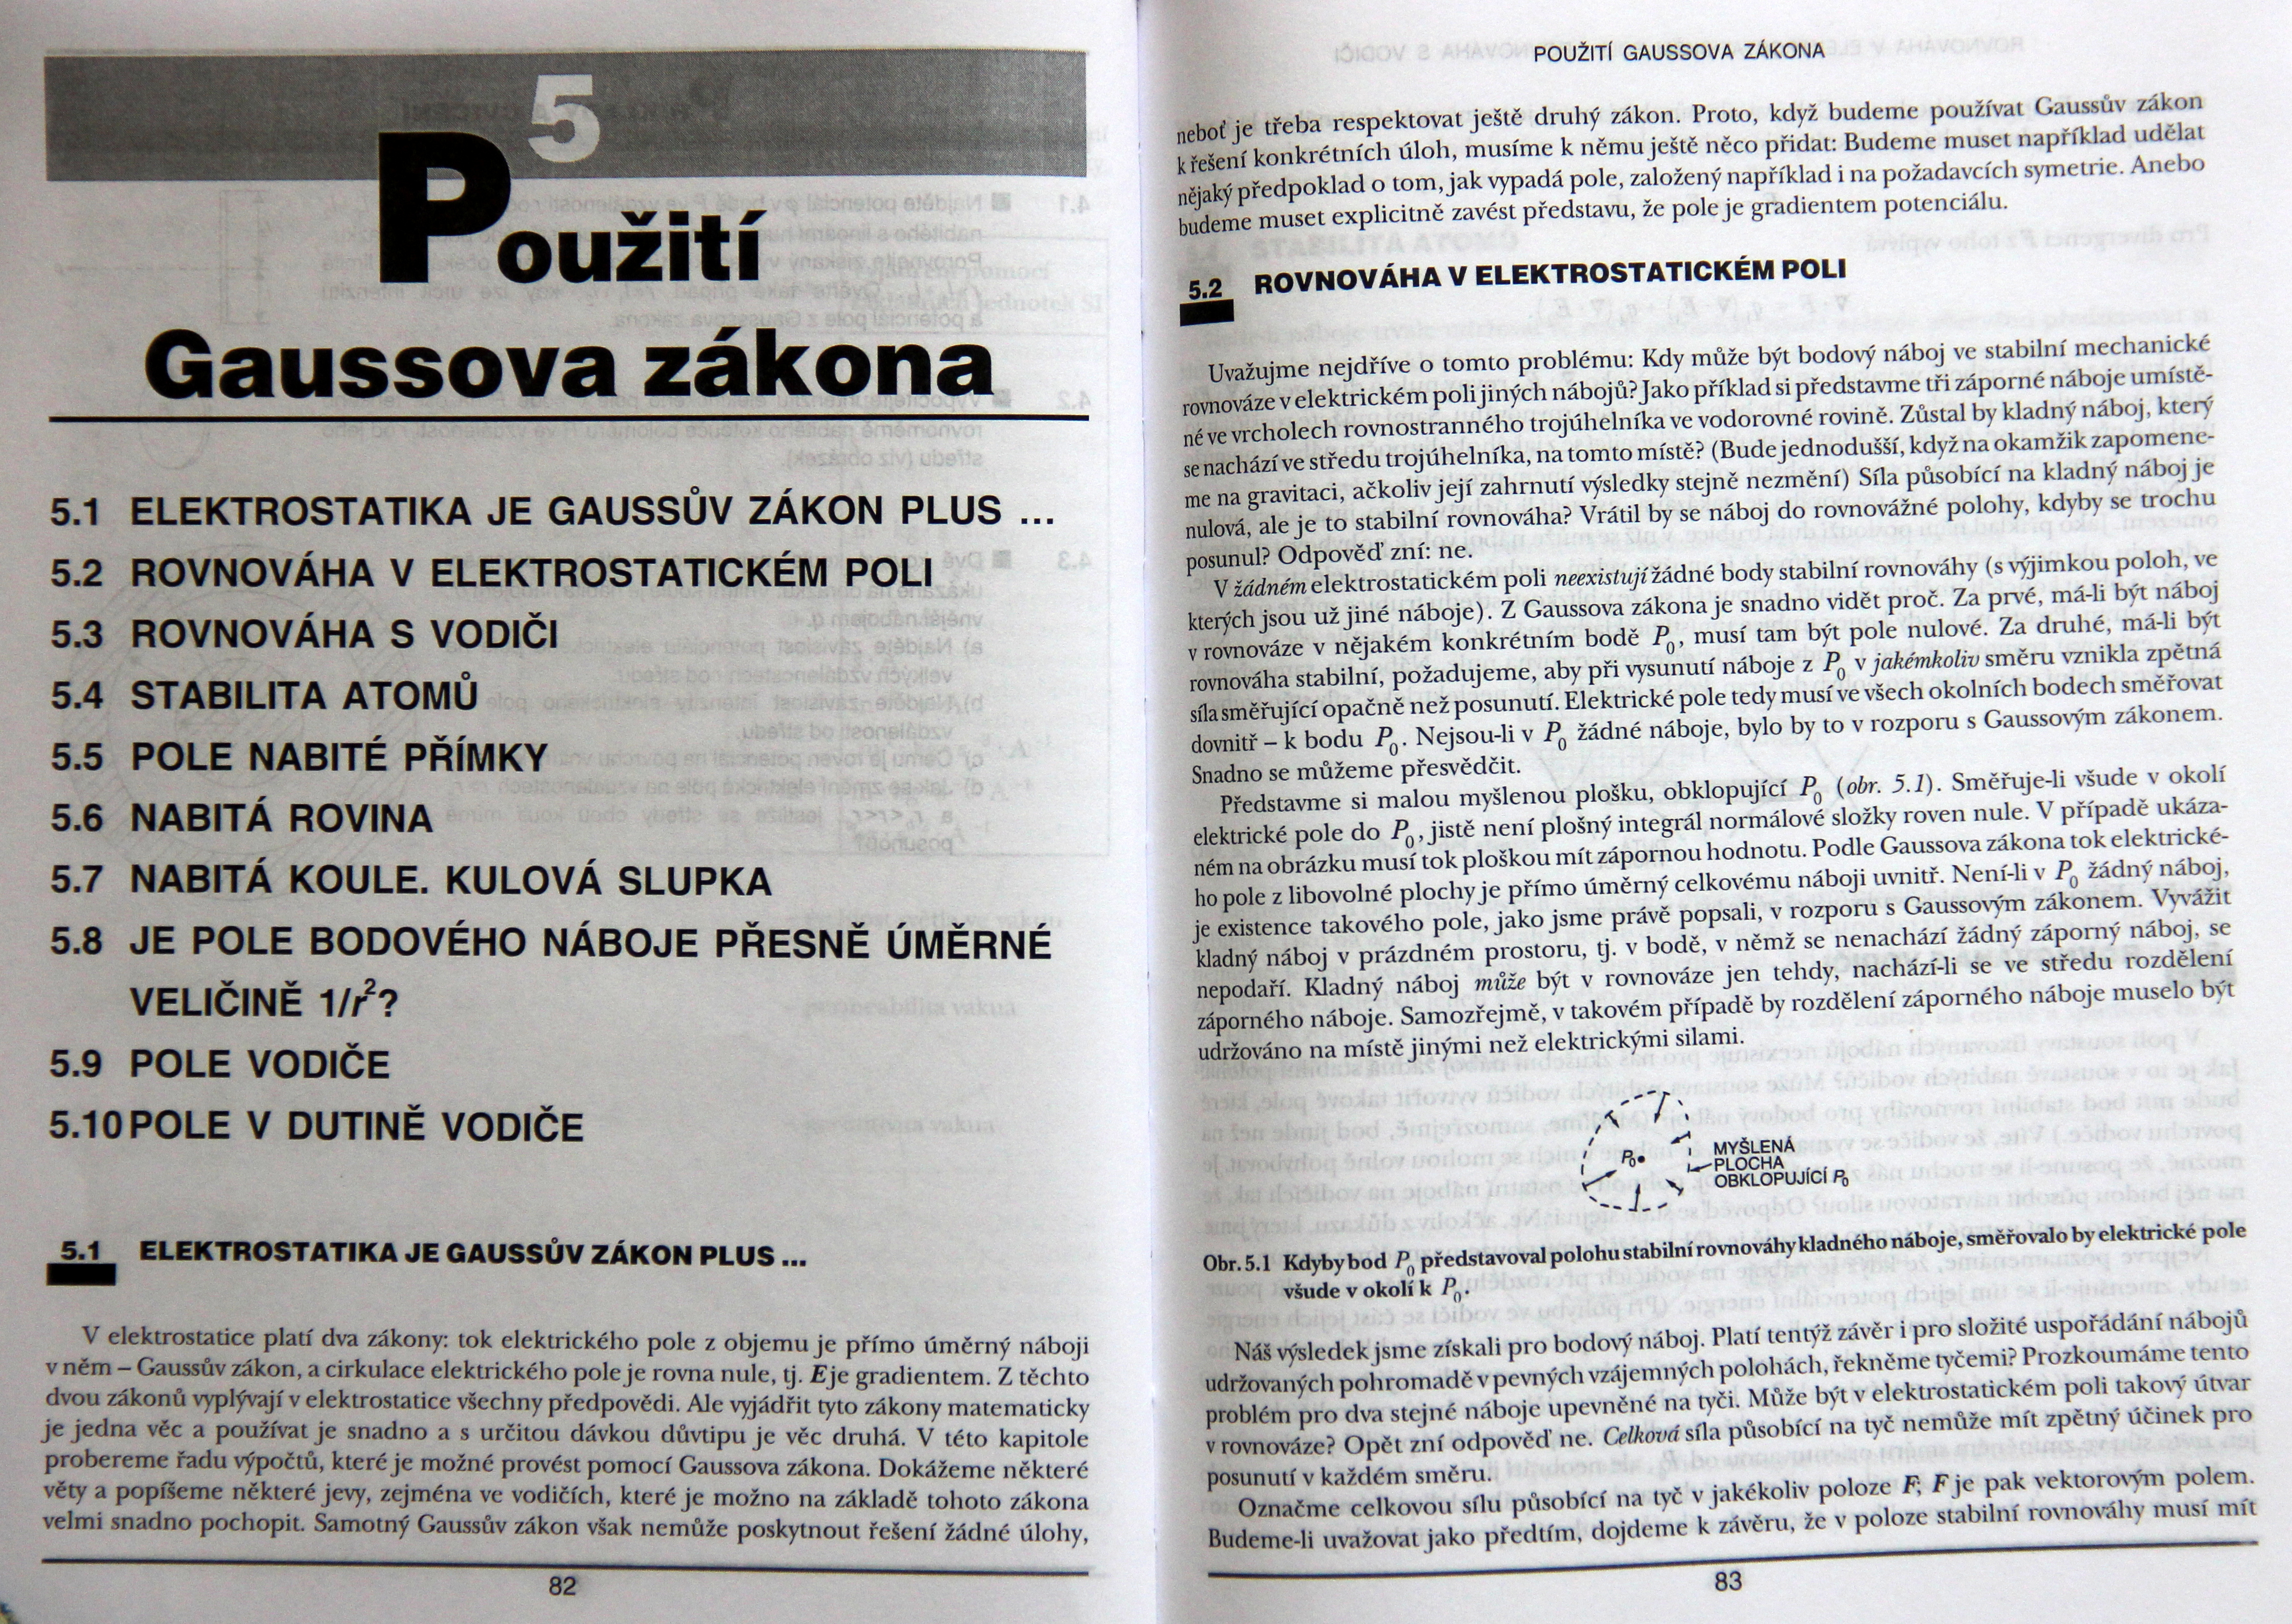
\includegraphics[width=0.6\linewidth]{fey_elstat_gauss01.jpg}
        \caption{Kdyby bod \(R\) představoval polohu stabilní rovnováhy kladného náboje, směřovalo by   
                 elektrické pole všude v okolí k \(P_0\).}
        \label{fyz:fig_fey_elstat_gauss01}
      \end{wrapfigure} 
      
      Označme celkovou sílu působící na tyč v jakékoliv poloze \(\vec{F}\); \(\vec{F}\) je pak vektorovým	
      polem. Budeme-li uvažovat jako předtím, dojdeme k závěru, že v poloze stabilní rovnováhy musí mít
      divergence \(\vec{F}\) zápornou hodnotu. Celková síla působící na tyč je rovna prvnímu náboji krát pole 
      v jeho poloze, plus druhý náboj krát pole v jeho poloze: 
      \begin{equation}\label{fyz:eq_fey_elstat_gauss01}
       \vec{F}=q_1\vec{E_1} + q_2\vec{E_2}. 
      \end{equation}
      Pro divergenci \(F\) z toho vyplývá \[\ndiver{F}=q_1(\ndiver{E_1}) + q_2(\ndiver{E_2}).\] Je-li každý z 
      těchto nábojů ve vakuu, jsou V \(q_1(\ndiver{E_1})\), stejně jako \(q_2(\ndiver{E_2})\) rovny nule a 
      divergence \(\ndiver{F}\) je také rovna nule - není tedy záporná, jak by bylo žádoucí pro rovnováhu. 
      Sami můžete rozšířit tuto úvahu a přesvědčit se, že vůbec žádný pevný útvar skládající se z jakéhokoliv 
      počtu nábojů nemůže mít v elektrostatickém poli polohu stabilní rovnováhy ve volném prostoru.
      
      Nedokázali jsme však, že rovnováha je zakázána, existují-li úchyty nebo jiná mechanická omezení. Jako 
      příklad nám poslouží dutá trubice, v níž se může náboj volně pohybovat dopředu a dozadu, ale ne do 
      stran. V tomto případě je možno velmi snadno navrhnout elektrické pole, které na obou koncích směřuje 
      dovnitř, připustí-li se, že v blízkosti středu trubice může směřovat ven do stran. Prostě na každý 
      konec trubice umístíme kladné náboje, jak ukazuje obr. \ref{fyz:fig_fey_elstat_gauss02}. Nyní může 
      existovat rovnovážný bod i tehdy, když je divergence rovna nule. Náboj by, samozřejmě, nebyl ve 
      stabilní rovnováze pro pohyb do stran, kdyby nepůsobily „neelektrické“ síly stěn trubice. 
      
      \begin{figure}[ht!] % \ref{fyz:fig_fey_elstat_gauss02}
        \centering
        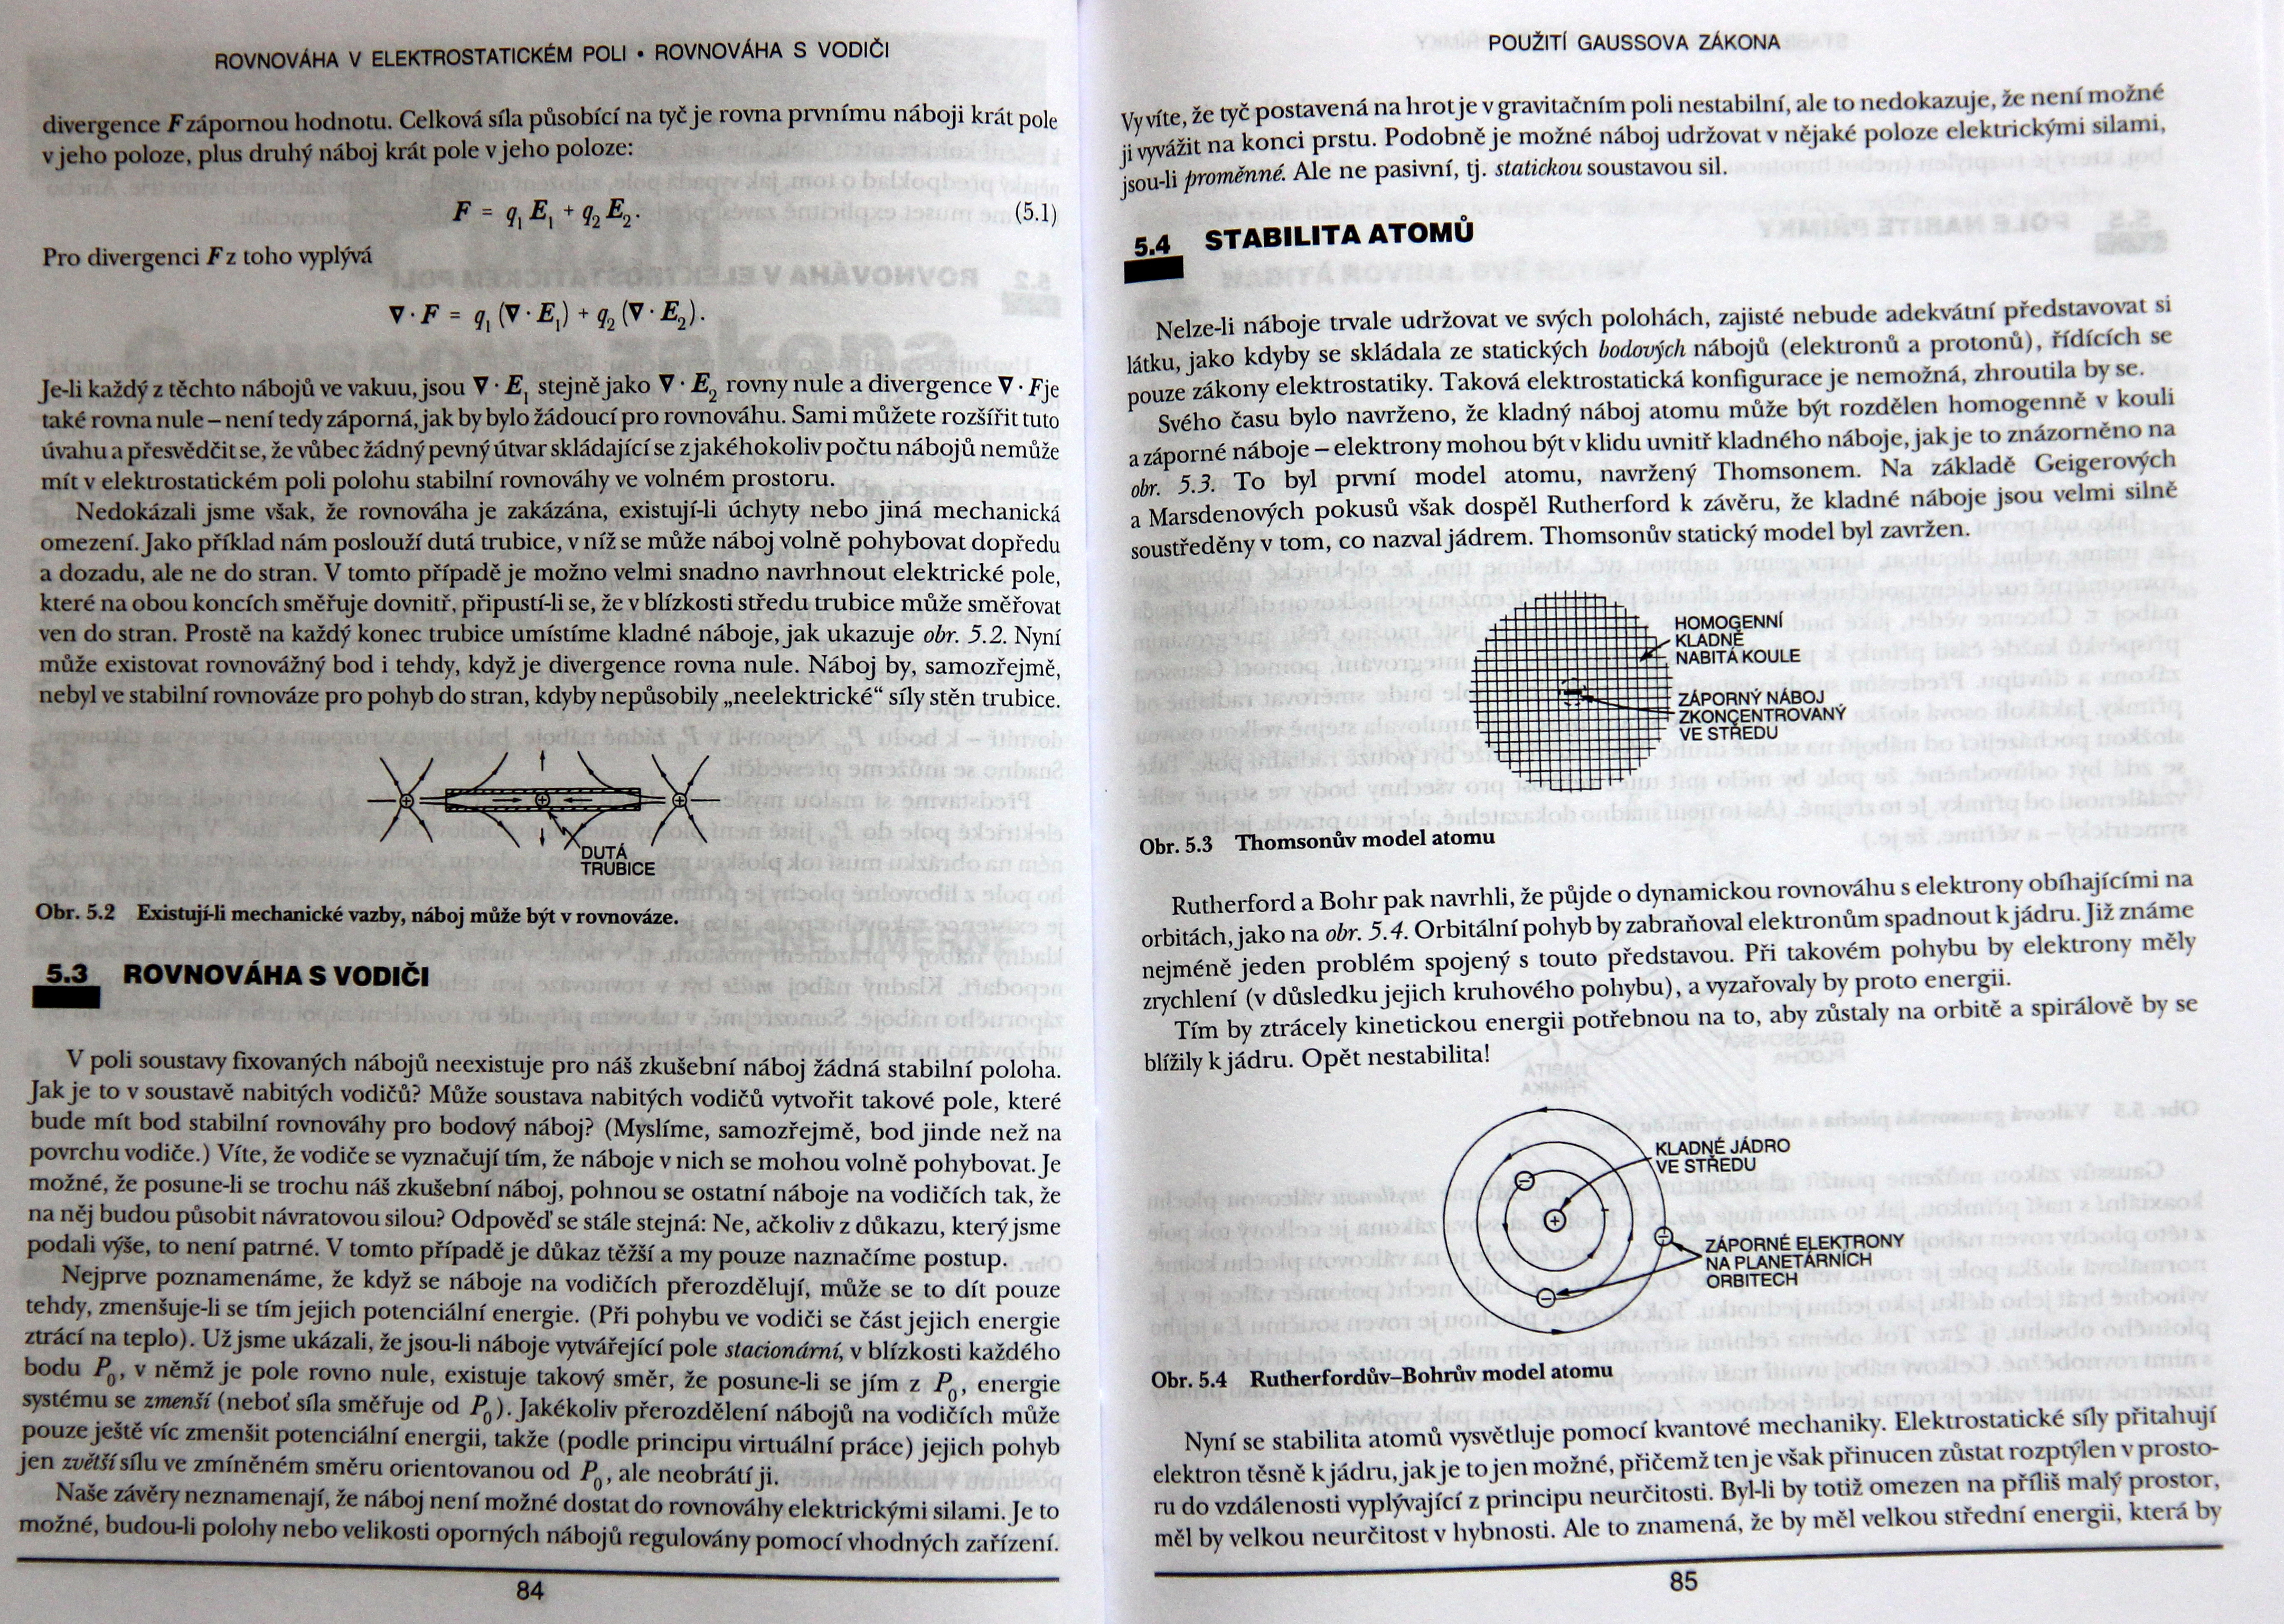
\includegraphics[width=0.6\linewidth]{fey_elstat_gauss02.jpg}
        \caption{Existují-li mechanické vazby, náboj může být v rovnováze.}
        \label{fyz:fig_fey_elstat_gauss02}
      \end{figure}      
      
    \subsection{Rovnováha s vodiči}
      V poli soustavy fixovaných nábojů neexistuje pro náš zkušební náboj žádná stabilní poloha. Jak je to v 
      soustavě nabitých vodičů? Může soustava nabitých vodičů vytvořit takové pole, které bude mít bod 
      stabilní rovnováhy pro bodový náboj? (Myslíme, samozřejmě, bod jinde než na povrchu vodiče.) Víte, že 
      vodiče se vyznačují tím, že náboje v nich se mohou volně pohybovat. Je možné, že posune-li se trochu 
      náš zkušební náboj, pohnou se ostatní náboje na vodičích tak, že na něj budou působit návratovou silou? 
      Odpověď se stále stejná: Ne, ačkoliv z důkazu, který jsme podali výše, to není patrné. V tomto případě 
      je důkaz těžší a my pouze naznačíme postup.
      
      \emph{Nejprve poznamenáme, že když se náboje na vodičích přerozdělují, může se to dít pouze tehdy, 
      zmenšuje-li se tím jejich potenciální energie}. (Při pohybu ve vodiči se část jejich energie ztrácí na 
      teplo). Už jsme ukázali, že jsou-li náboje vytvářející pole \emph{stacionární}, v blízkosti každého 
      bodu \(P_0\), v němž je pole rovno nule, existuje takový směr, že posune-li se jím z \(P_0\), energie 
      systému se zmenší (neboť síla směřuje od \(P_0\)). Jakékoliv přerozdělení nábojů na vodičích může pouze 
      ještě víc zmenšit potenciální energii, takže (podle principu virtuální práce) jejich pohyb jen zvětší 
      sílu ve zmíněném směru orientovanou od \(P_0\), ale neobrátí ji.
      
      Naše závěry neznamenají, že náboj není možné dostat do rovnováhy elektrickými silami. Je to možné, 
      budou-li polohy nebo velikosti opěrných nábojů regulovány pomocí vhodných zařízení. Vy víte, že tyč 
      postavená na hrot je v gravitačním poli nestabilní, ale to nedokazuje, že není možné ji vyvážit na 
      konci prstu. Podobně je možné náboj udržovat v nějaké poloze elektrickými silami, jsou-li 
      \emph{proměnné}. Ale ne pasivní, tj. \emph{statickou} soustavou sil.
    
    \subsection{Stabilita atomů}
      Nelze-li náboje trvale udržovat ve svých polohách, zajisté nebude adekvátní představovat si látku, jako 
      kdyby se skládala ze statických bodových nábojů (elektronů a protonů), řídících se pouze zákony 
      elektrostatiky. Taková elektrostatická konfigurace je nemožná, zhroutila by se.
      
      Svého času bylo navrženo, že kladný náboj atomu může být rozdělen homogenně v kouli a záporné náboje — 
      elektrony mohou být v klidu uvnitř kladného náboje, jak je to znázorněno na obr. 
      \ref{fyz:fig_fey_elstat_gauss03}. To byl první model atomu, navržený Thomsonem. Na základě Geigerových 
      a Marsdenových pokusů však dospěl Rutherford k závěru, že kladné náboje jsou velmi silně soustředěny v 
      tom, co nazval jádrem. Thomsonův statický model 
      byl zavržen.
      \begin{figure}[ht!] % \ref{fyz:fig_fey_elstat_gauss03}
        \centering
        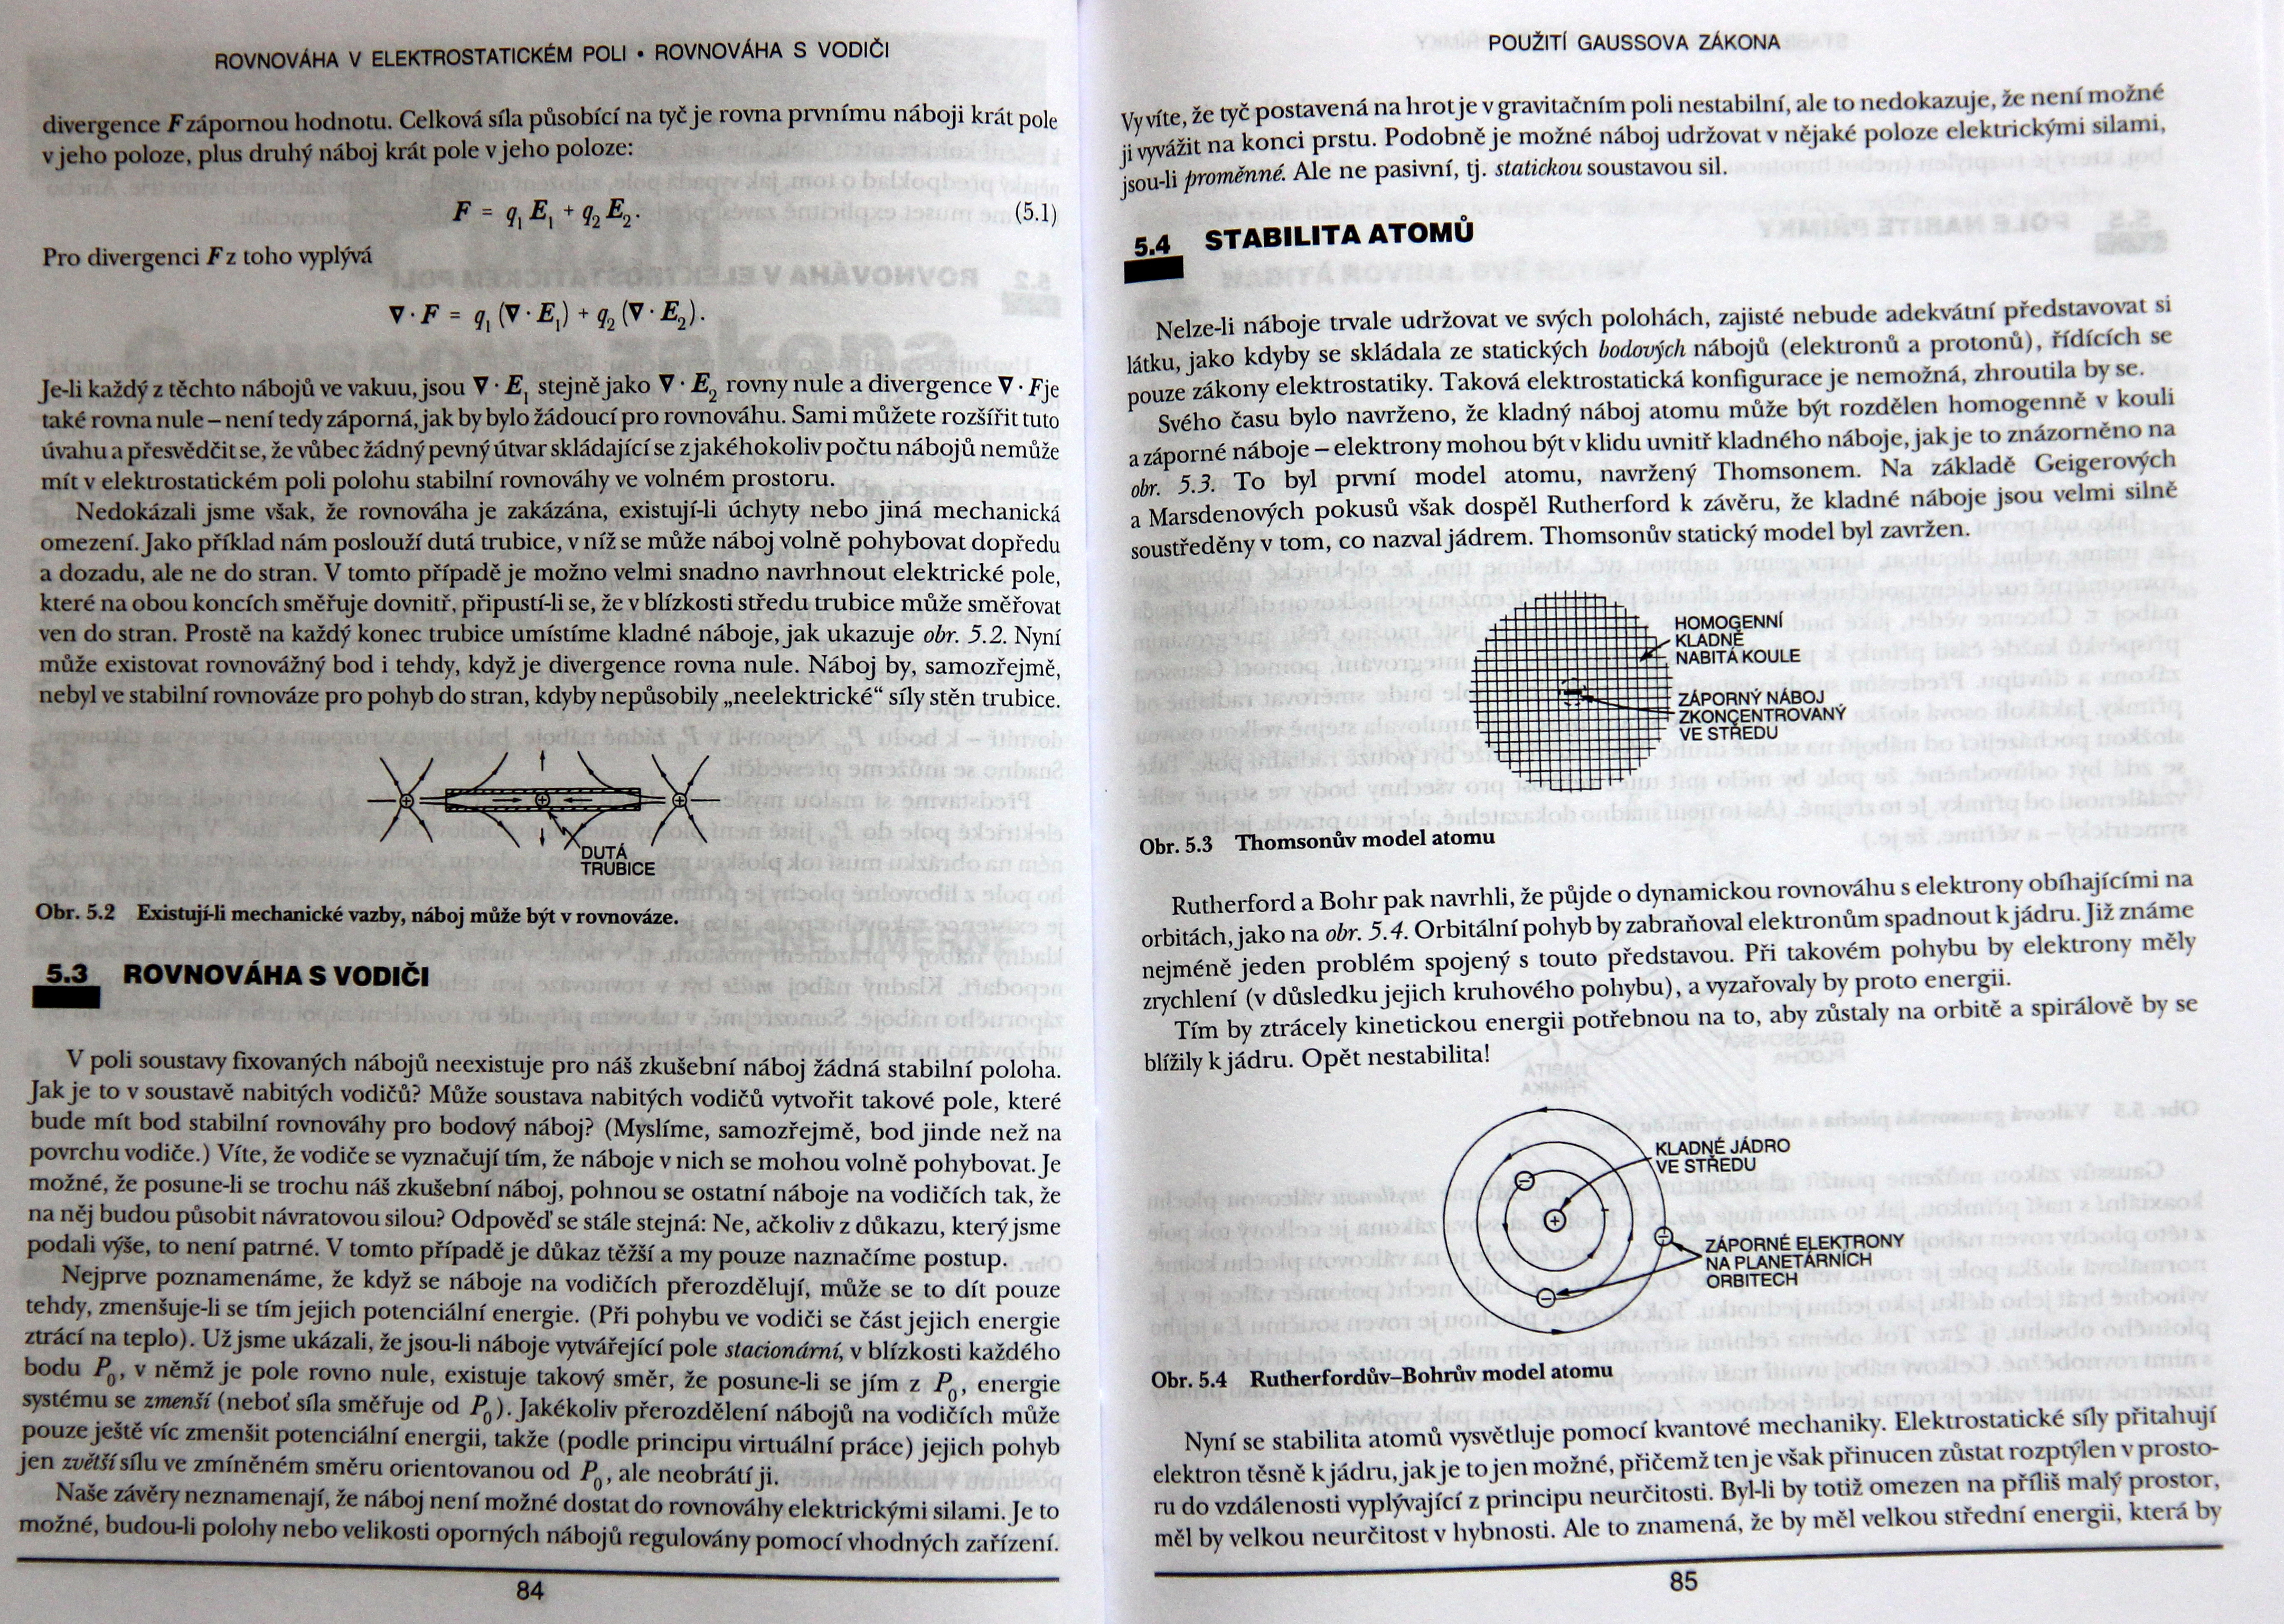
\includegraphics[width=0.6\linewidth]{fey_elstat_gauss03.jpg}
        \caption{Thomsonův model atomu}
        \label{fyz:fig_fey_elstat_gauss03}
      \end{figure}
      
      Rutherford a Bohr pak navrhli, že půjde o dynamickou rovnováhu s elektrony obíhajícími na orbitách, 
      jako na obr. \ref{fyz:fig_fey_elstat_gauss04}. Orbitální pohyb by zabraňoval elektronům spadnout k 
      jádru. Již známe nejméně jeden problém spojený s touto představou. Při takovém pohybu by elektrony měly 
      zrychlení (v důsledku jejich kruhového pohybu), a vyzařovaly by proto energii.
      
      Tím by ztrácely kinetickou energii potřebnou na to, aby zůstaly na orbitě a spirálově by se blížily k 
      jádru. Opět nestabilita!
      \begin{figure}[ht!] % \ref{fyz:fig_fey_elstat_gauss04}
        \centering
        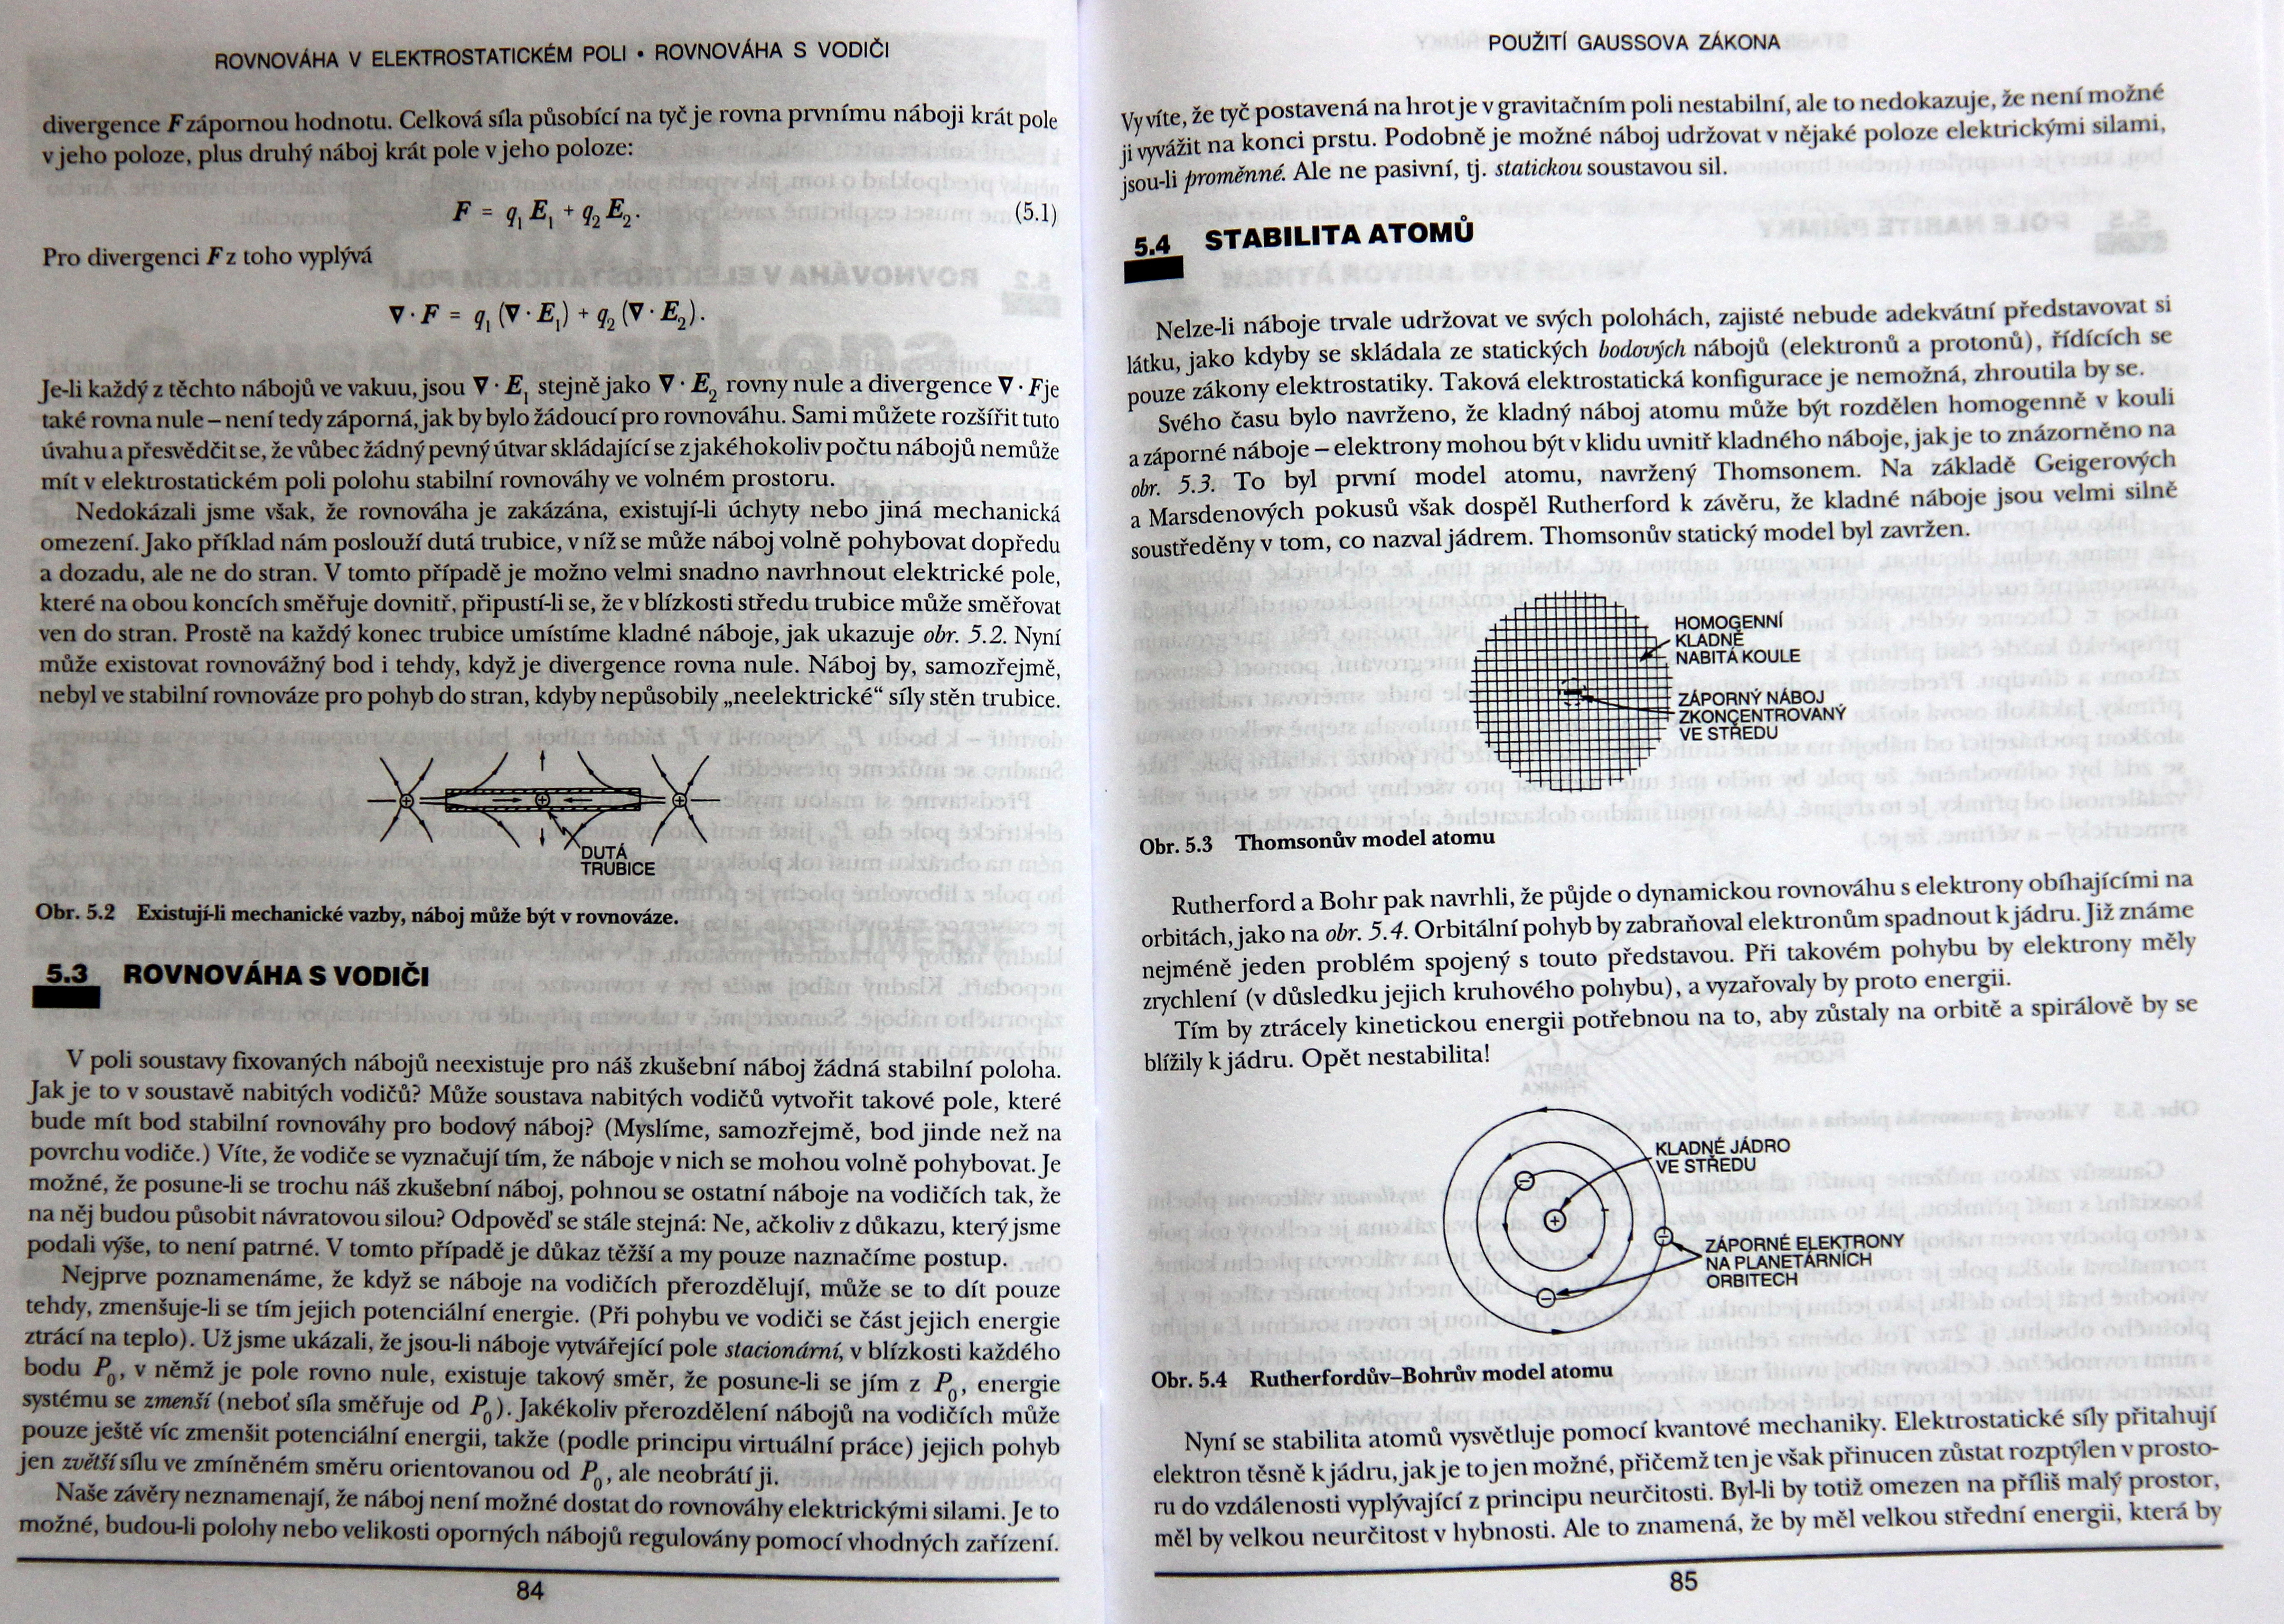
\includegraphics[width=0.6\linewidth]{fey_elstat_gauss04.jpg}
        \caption{Rutherfordův-Bohrův model atomu}
        \label{fyz:fig_fey_elstat_gauss04}
      \end{figure}      
      
      Nyní se stabilita atomů vysvětluje pomocí kvantové mechaniky. Elektrostatické síly přitahují elektron 
      těsně k jádru, jak je to jen možné, přičemž ten je však přinucen zůstat rozptýlen v prostoru do 
      vzdálenosti vyplývající z principu neurčitosti. Byl-li by totiž omezen na příliš malý prostor, měl by 
      velkou neurčitost v hybnosti. Ale to znamená, že by měl velkou střední energii, která by mu umožňovala 
      vymanit se z elektrické přitažlivosti jádra. Konečným výsledkem je taková elektrická rovnováha, která 
      se ani příliš neliší od Thomsonovy představy - pouze je to záporný náboj, který je rozptýlen (neboť 
      hmotnost elektronu je mnohokrát menší než hmotnost protonu).
    
    \subsection{Pole nabité přímky}
      Gaussův zákon je možno použít na řešení mnoha úloh o elektrostatickém poli vyznačujících se speciální 
      symetrií - obvykle kulovou, válcovou nebo rovinnou. Ve zbývající částí této kapitoly použijeme Gaussův 
      zákon v několika takových úlohách. Snadnost, s jakou lze tyto úlohy takto řešit, může vést ke klamnému 
      dojmu, že jde o velmi účinnou metodu umožňující postupovat tak i v mnoha dalších úlohách. Naneštěstí 
      tomu tak není. Seznam úloh, které lze pomocí Gaussova zákona snadno řešit, bude brzy vyčerpán. V 
      dalších kapitolách vypracujeme účinnější metody ke zkoumání elektrostatických polí.
      
      Jako náš první příklad budeme uvažovat soustavu s válcovou souměrností. Předpokládejme, že máme velmi 
      dlouhou, homogenně nabitou tyč. Myslíme tím, že elektrické náboje jsou rovnoměrně rozděleny podél 
      nekonečně dlouhé přímky, přičemž na jednotkovou délku připadá náboj \(\tau\). Chceme vědět, jaké bude 
      elektrické pole. Úlohu je jistě možno řešit integrováním příspěvků každé části přímky k poli. My to 
      však dokážeme bez integrování, pomocí Gaussova zákona a důvtipu. Především snadno vytušíme, že 
      elektrické pole bude směřovat radiálně od přímky. Jakákoli osová složka nábojů na jedné straně by se 
      totiž anulovala stejně velkou osovou složkou pocházející od nábojů na straně druhé. Výsledkem může být 
      pouze radiální pole. Také se zdá být odůvodněné, že pole by mělo mít tutéž velikost pro všechny body ve 
      stejně velké vzdálenosti od přímky. Je to zřejmé. (Asi to není snadno dokazatelné, ale je to pravda, 
      je-li prostor symetrický - a věříme, že je.)
      
      \begin{figure}[ht!] % \ref{fyz:fig_fey_elstat_gauss05}
        \centering
        \includegraphics[width=0.6\linewidth]{fey_elstat_gauss05.jpg}
        \caption{Válcová gaussovská plocha s nabitou přímkou v ose}
        \label{fyz:fig_fey_elstat_gauss05}
      \end{figure}  
      
      Gaussův zákon můžeme použít následujícím způsobem. Mějme myšlenou válcovou plochu koaxiální s naší 
      přímkou, jak to znázorňuje obr. \ref{fyz:fig_fey_elstat_gauss05}. Podle Gaussova zákona je celkový tok 
      pole z této plochy roven náboji uvnitř válce, dělenému \(\varepsilon_0\). Protože pole je na válcovou 
      plochu kolmé, normálová složka pole je rovna velikosti pole. Označíme ji \(E\). Dále nechť poloměr 
      válce je \(r\). Je výhodné brát jeho délku jako jednotkovou. Tok válcovou plochou je roven součinu 
      \(E\) a jejího plošného obsahu, tj. \(2\pi r\). Tok oběma čelními stěnami je roven nule, protože 
      elektrické pole je s nimi rovnoběžné. Celkový náboj uvnitř naší válcové plochy je přesně \(\tau\), 
      neboť délka části přímky uzavřené uvnitř válce je rovna jedné jednotce. Z Gaussova zákona pak vyplývá, 
      že
      \begin{equation}\label{fyz:eq_fey_elstat_gauss02}
        E\cdot2\pi r = \frac{\tau}{\varepsilon_0} \Rightarrow E = \frac{\tau}{2\pi\varepsilon_0 r}
      \end{equation}
      Elektrické pole nabité přímky je nepřímo úměrné \emph{první} mocnině vzdálenosti od přímky.
    
    \subsection{Nabitá rovina, dvě roviny}
      V dalším příkladě budeme počítat pole homogenně nabité roviny. Předpokládejme, že rovina se rozprostírá 
      do nekonečna a na její plošnou jednotku připadá náboj \(\sigma\). Teď provedeme další odhad. Důvody 
      souměrnosti nás totiž vedou k přesvědčení, že směr pole je všude kolmý na rovinu a že 
      \emph{neexistuje-li pole jiných nábojů}, musí být pole na obou stranách roviny stejné (co do 
      velikostí). Tentokrát zvolme jako naši gaussovskou plochu pravoúhlou krabičku, která protíná uvažovanou 
      rovinu (obr. \ref{fyz:fig_fey_elstat_gauss06}). Stěny krabičky rovnoběžné s rovinou budou mít stejný 
      plošný obsah \(S\). Pole je na tyto dvě stěny kolmé a se zbývajícími čtyřmi stěnami je rovnoběžné. 
      Celkový tok je roven \(E-\text{krát}\) plošnému obsahu první stěny plus \(E-\text{krát}\) plošný obsah 
      protilehlé stěny, přičemž zbývající čtyři stěny nepřispívají ničím. Celkový náboj uvnitř krabičky je 
      \(\sigma\cdot S\). Když jej uvedeme do vztahu s tokem stěnami krabice, dostaneme rovnost
      \begin{equation}\label{fyz:eq_fey_elstat_gauss03}
        E\cdot S + E\cdot S = \frac{\sigma\cdot S}{\varepsilon_0} \Rightarrow 
        E = \frac{\sigma}{2\varepsilon_0}.
      \end{equation}
      
      \begin{figure}[ht!] % \ref{fyz:fig_fey_elstat_gauss06}
        \centering
        \includegraphics[width=0.6\linewidth]{fey_elstat_gauss06.jpg}
        \caption{Elektrické pole v blízkosti homogenně nabité roviny je možno najít použitím Gaussova zákona 
                 na myšlenou krabici.}
        \label{fyz:fig_fey_elstat_gauss06}
      \end{figure}
      
      Tentýž výsledek jsme dostali už dříve integrováním po celé ploše. Gaussův zákon nám dává odpověď v 
      tomto příkladě o mnoho rychleji (ačkoli nemá takovou obecnou použitelnost jako dřívější metoda).
      
      Zdůrazňujeme, že tento výsledek se vztahuje pouze na pole vytvořené náboji rozmístěnými v rovině. 
      Nacházejí-li se někde v blízkostí ještě další náboje, bude celkové pole v okolí roviny rovno součtu 
      pole (\ref{fyz:eq_fey_elstat_gauss03}) a pole pocházejícího od těchto nábojů.
      
      Úloha se dvěma rovnoběžnými rovinami se stejnými plošnými hustotami nábojů, které mají opačná znaménka 
      \(+\sigma\) a \(-\sigma\), je také jednoduchá, předpokládáme-li opět, že vnější svět je zcela souměrný. 
      Superpozicí obou řešení pro jednotlivé roviny nebo sestrojením gaussovské krabice, která by proťala obě 
      roviny, je možno jednoduše ozřejmit, že na vnější straně rovin je pole rovno nule (obr. 
      \ref{fyz:fig_fey_elstat_gauss07}a). Kdybychom uvažovali krabici, která protíná jen jednu z rovin částí 
      b, c obrázku), mohli bychom se přesvědčit, že pole mezi deskami musí být dvakrát větší než v případě 
      jedni desky. Podle Gaussova zákona by pak platilo, že
      \begin{equation}\label{fyz:eq_fey_elstat_gauss04}
        E_1 + E_2 = \frac{\sigma}{\varepsilon_0}
      \end{equation}
      kde \(E_1\) a \(E_1\) jsou pole na každé straně roviny směřující od ní.
      \begin{figure}[ht!] % \ref{fyz:fig_fey_elstat_gauss07}
        \centering
        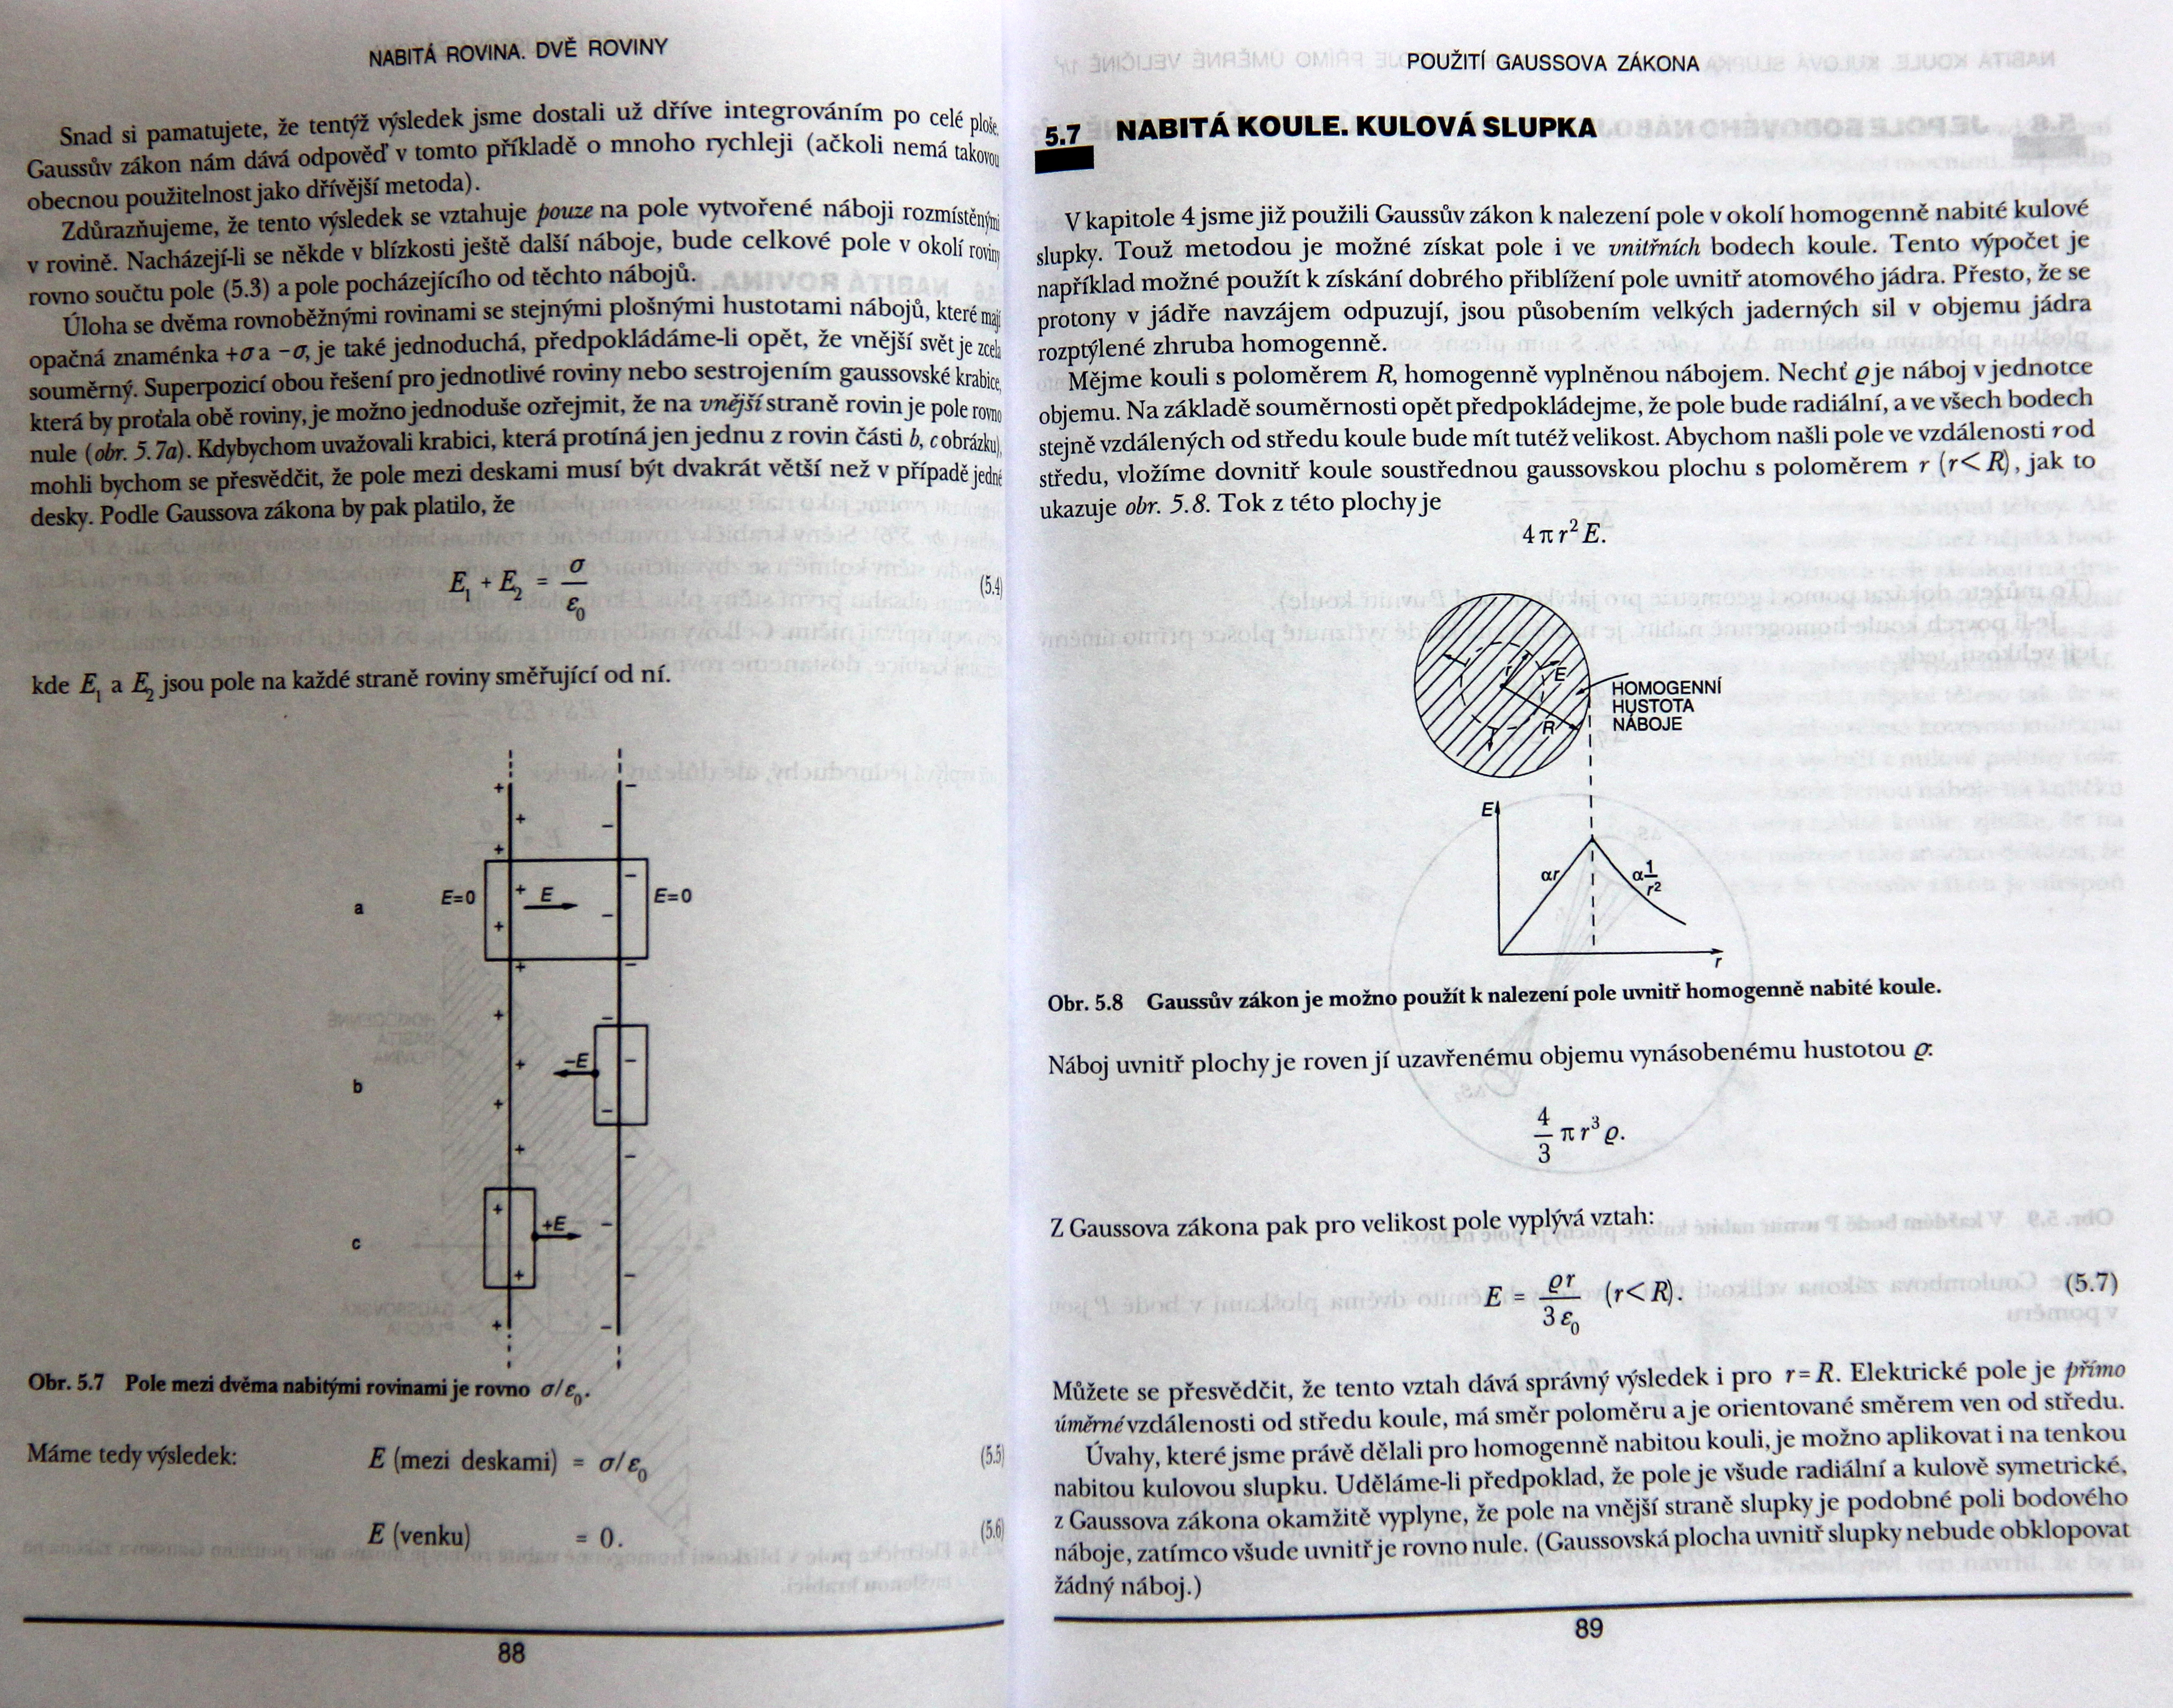
\includegraphics[width=0.6\linewidth]{fey_elstat_gauss07.jpg}
        \caption{Pole mezi dvěma nabitými rovinami je rovno \(\frac{\sigma}{\varepsilon_0}\)}
        \label{fyz:fig_fey_elstat_gauss07}
      \end{figure}
      Máme tedy výsledek
      \begin{align}
        E (\text{mezi deskami}) &= \frac{\sigma}{\varepsilon_0} \\
        E (\text{venku})        &= 0  
      \end{align}
      
    \subsection{Nabitá koule, kulová slupka}
      V kapitole \ref{fyz:chap_fey_ponako} jsme již použili Gaussův zákon k nalezení pole v okolí homogenně 
      nabité kulové slupky. Touž metodou je možné získat pole i ve vnitřních bodech koule. Tento výpočet je 
      například možné použít k získání dobrého přiblížení pole uvnitř atomového jádra. Přesto, že se protony 
      v jádře navzájem odpuzují, jsou působením velkých jaderných sil v objemu jádra rozptýlené zhruba 
      homogenně.
      
      Mějme kouli s poloměrem \(R\), homogenně vyplněnou nábojem. Nechť \(\varrho\) je náboj v jednotce 
      objemu. Na základě souměrnosti opět předpokládejme, že pole bude radiální, a ve všech bodech stejně 
      vzdálených od středu koule bude mít tutéž velikost. Abychom našli pole ve vzdálenosti \(r\) od středu, 
      vložíme dovnitř koule soustřednou gaussovskou plochu s poloměrem \(r\) \((r< R)\), jak to ukazuje obr. 
      \ref{fyz:fig_fey_elstat_gauss08}. Tok z této plochy je \[4\pi r^2E.\]
      \begin{figure}[ht!] % \ref{fyz:fig_fey_elstat_gauss08}
        \centering
        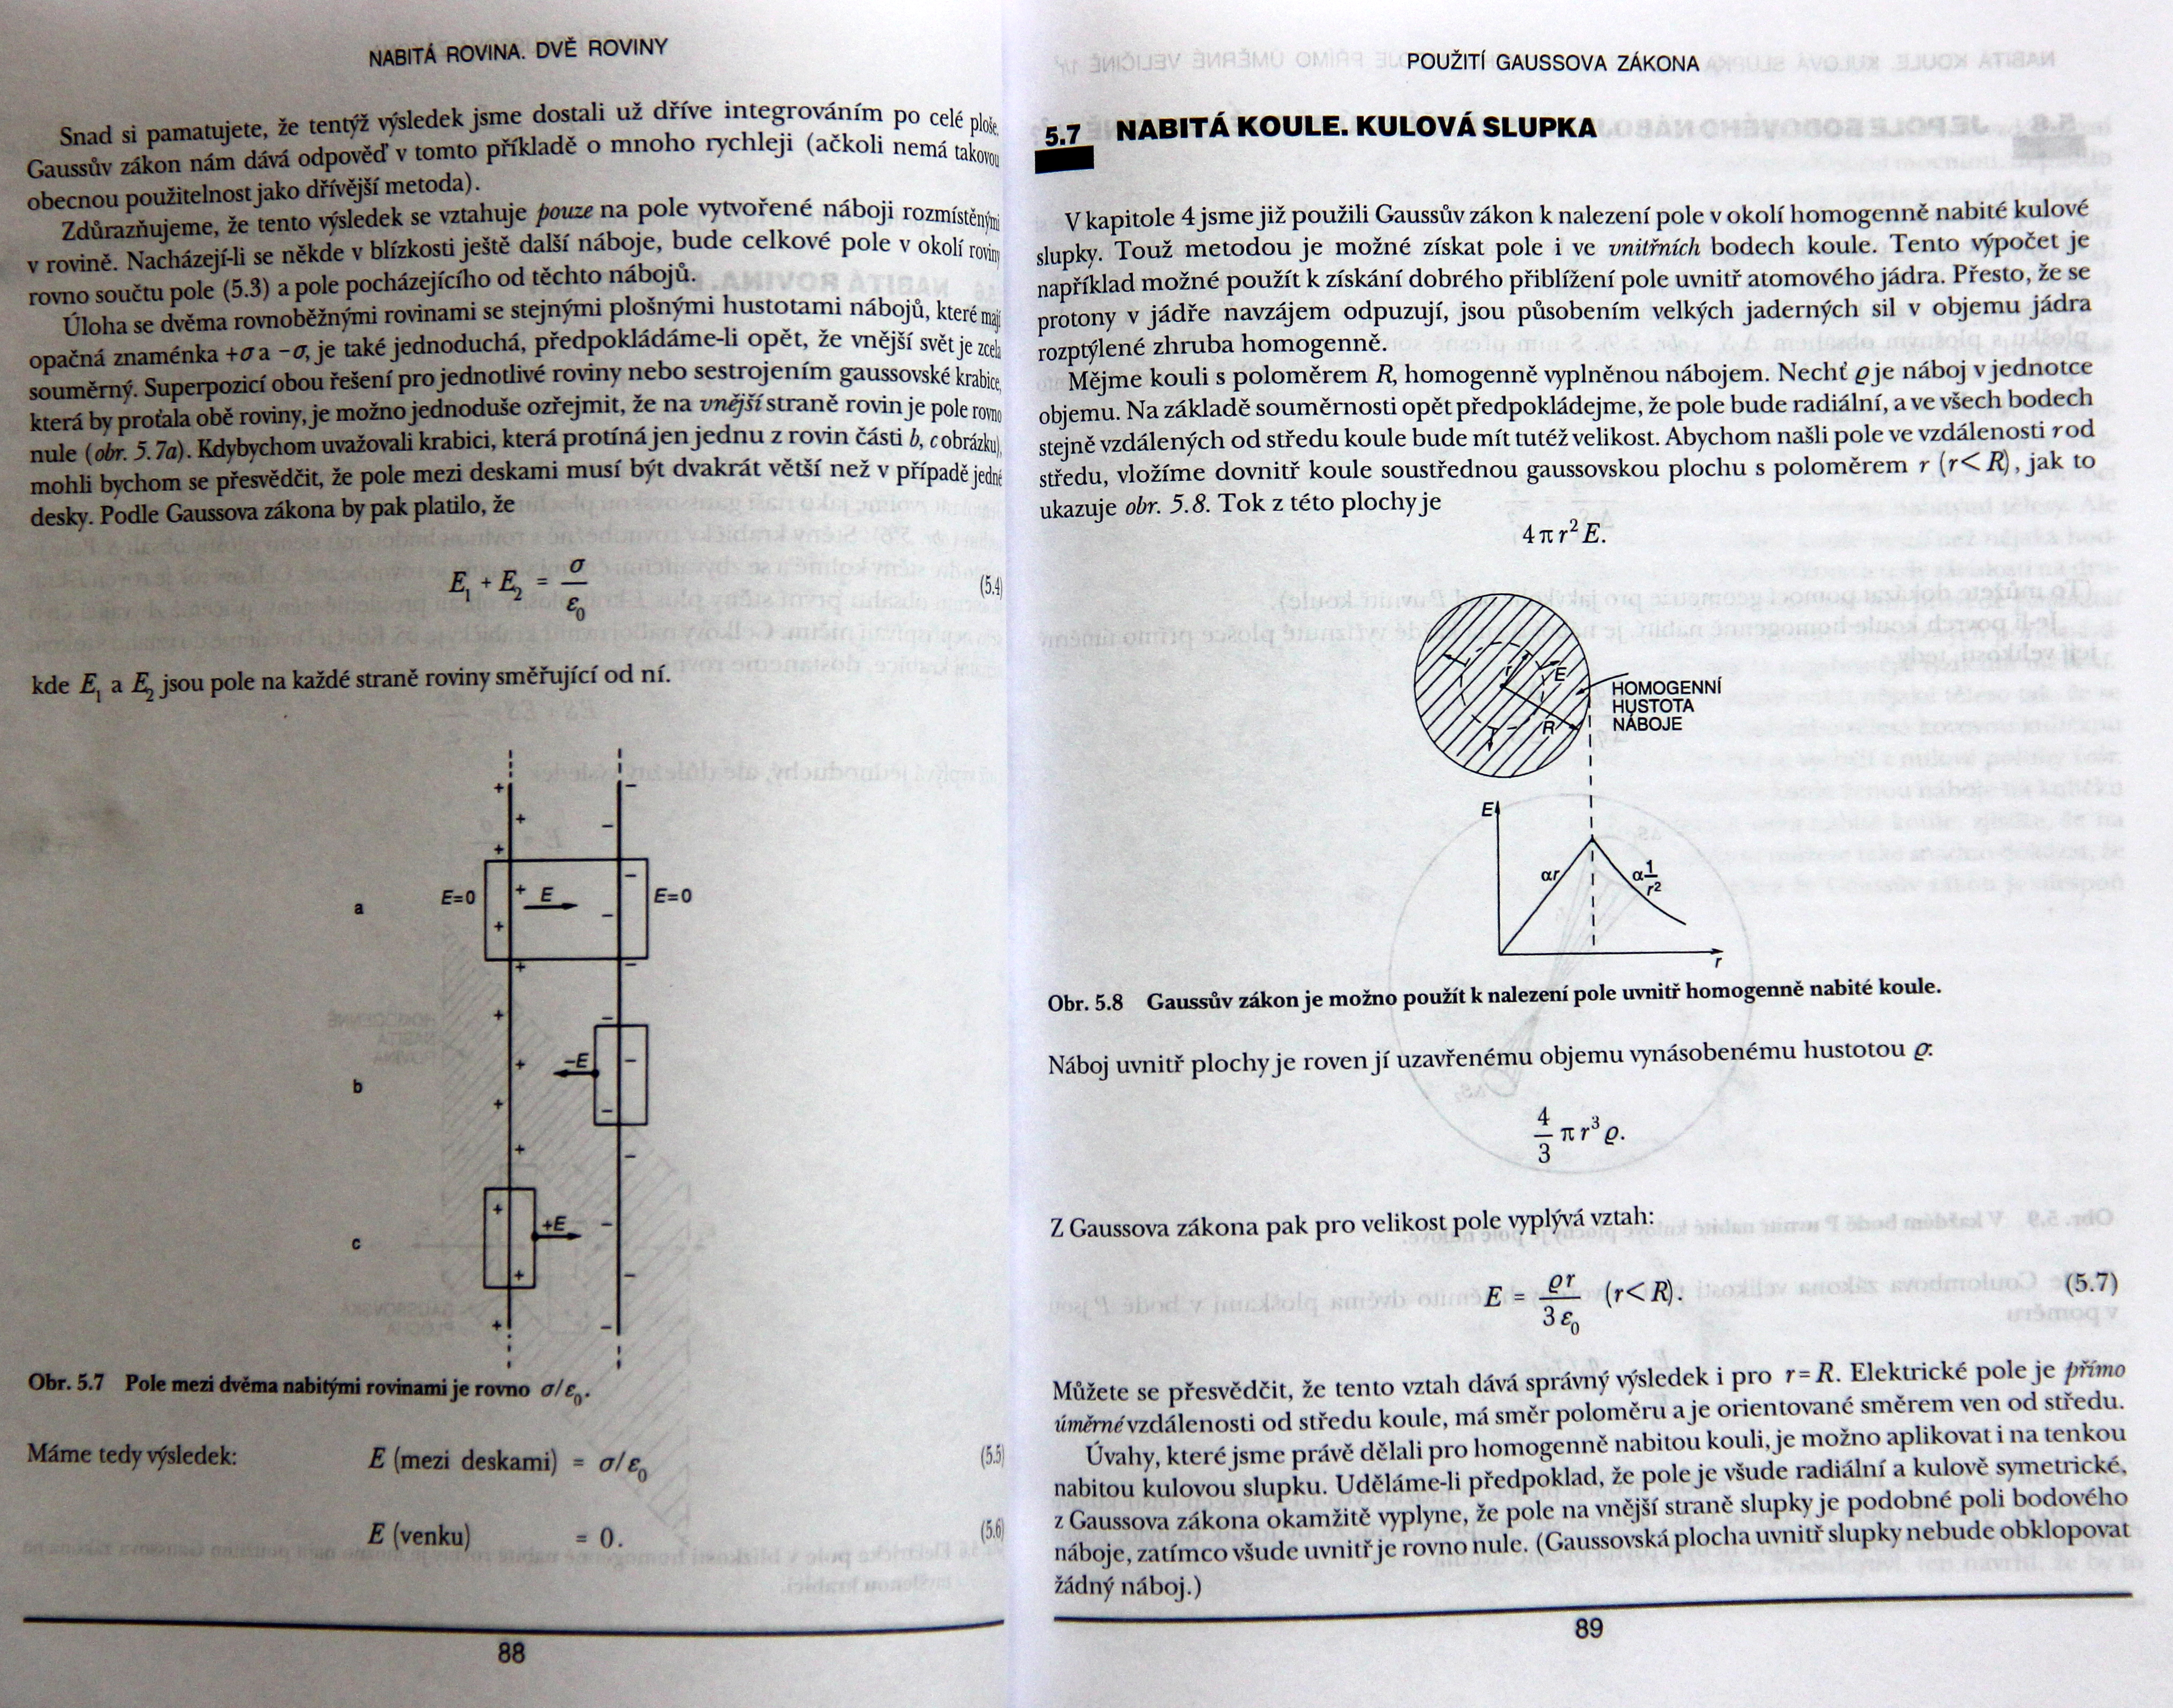
\includegraphics[width=0.6\linewidth]{fey_elstat_gauss08.jpg}
        \caption{Gaussův zákon je možno použít k nalezení pole uvnitř homogenně nabité koule.}
        \label{fyz:fig_fey_elstat_gauss08}
      \end{figure}
      Náboj uvnitř plochy je roven jí uzavřenému objemu vynásobenému hustotou \(\varrho\):
      \begin{align}
        Q_{\text{uvnitř}} 
                = \limitint_{\mathclap{\substack{\text{objem}\\
                                                 \text{uvnitř }S}}} \varrho\dd{V} 
          &= \frac{4}{3}\pi r^3\varrho.    \label{fyz:eq_fey_elstat_gauss05}    \\
       \shortintertext{Z Gaussova zákona pak pro velikost pole vyplývá vztah:}
       \limitint_S E_n\dd{S}
          &= \frac{Q_{\text{uvnitř}}}{\varepsilon_0} 
                \qquad\Rightarrow\qquad 4\pi r^2E 
                = \frac{4\pi r^3\varrho}{3\,\varepsilon_0}  \label{fyz:eq_fey_elstat_gauss06} \\ 
       \shortintertext{tedy:}
       E  &= \frac{\varrho r}{3\,\varepsilon_0} \qquad (r<R).
      \end{align}
      
      Můžete se přesvědčit, že tento vztah dává správný výsledek i pro \(r=R\). Elektrické pole je přímo 
      úměrné vzdálenosti od středu koule, má směr poloměru a je orientované směrem ven od středu.
      Úvahy, které jsme právě dělali pro homogenně nabitou kouli, je možno aplikovat i na tenkou nabitou 
      kulovou slupku. Uděláme-li předpoklad, že pole je všude radiální a kulově symetrické, z Gaussova zákona 
      okamžitě vyplyne, Že pole na vnější straně slupky je podobné poli bodového náboje, zatímco všude 
      uvnitř je rovno nule. (Gaussovská plocha uvnitř slupky nebude obklopovat žádný náboj.)
      
    \subsection{Je pole bodového náboje přesně přímo úměrné veličině 
                 \texorpdfstring{\(\frac{1}{r^2}\)}{1/r^2}?} 
      Podíváme-li se trochu podrobněji, jak se pole uvnitř kulové slupky stává nulovým, lépe si ozřejmíme, 
      proč platnost Gaussova zákona vyplývá právě jen z přesné závislosti Coulombovy síly na druhé mocnině 
      vzdálenosti. Uvažujme nějaký bod \(P\) uvnitř homogenně nabité kulové plochy. Představme si úzký kužel, 
      který má vrchol v \(P\) a sahá po kulovou plochu, na které vytíná malou plošku s plošným obsahem 
      \(\Delta S_1\) (obr. \ref{fyz:fig_fey_elstat_gauss09}). S ním přesně souměrný kužel vycházející z \(P\) 
      na opačnou stranu by na kulové ploše vyřízl plošku s obsahem \(\Delta S_2\). Jsou-li vzdálenosti od 
      \(P\) k těmto dvěma ploškám \(r_1\) a \(r_2\), jsou jejich plošné obsahy v poměru \[\frac{\Delta 
      S_2}{\Delta S_1} = \frac{r_2^2}{r_1^2}\]
      (To můžete dokázat pomocí geometrie pro jakýkoliv bod \(P\) uvnitř koule).
      
      Je-li povrch koule homogenně nabitý, je náboj \(\Delta q\) na každé vyříznuté plošce přímo úměrný její 
      velikosti, tedy \[\frac{\Delta q_2}{\Delta q_1} = \frac{\Delta S_2}{\Delta S_1}.\]
      
      
      \begin{figure}[ht!] % \ref{fyz:fig_fey_elstat_gauss09}
        \centering
        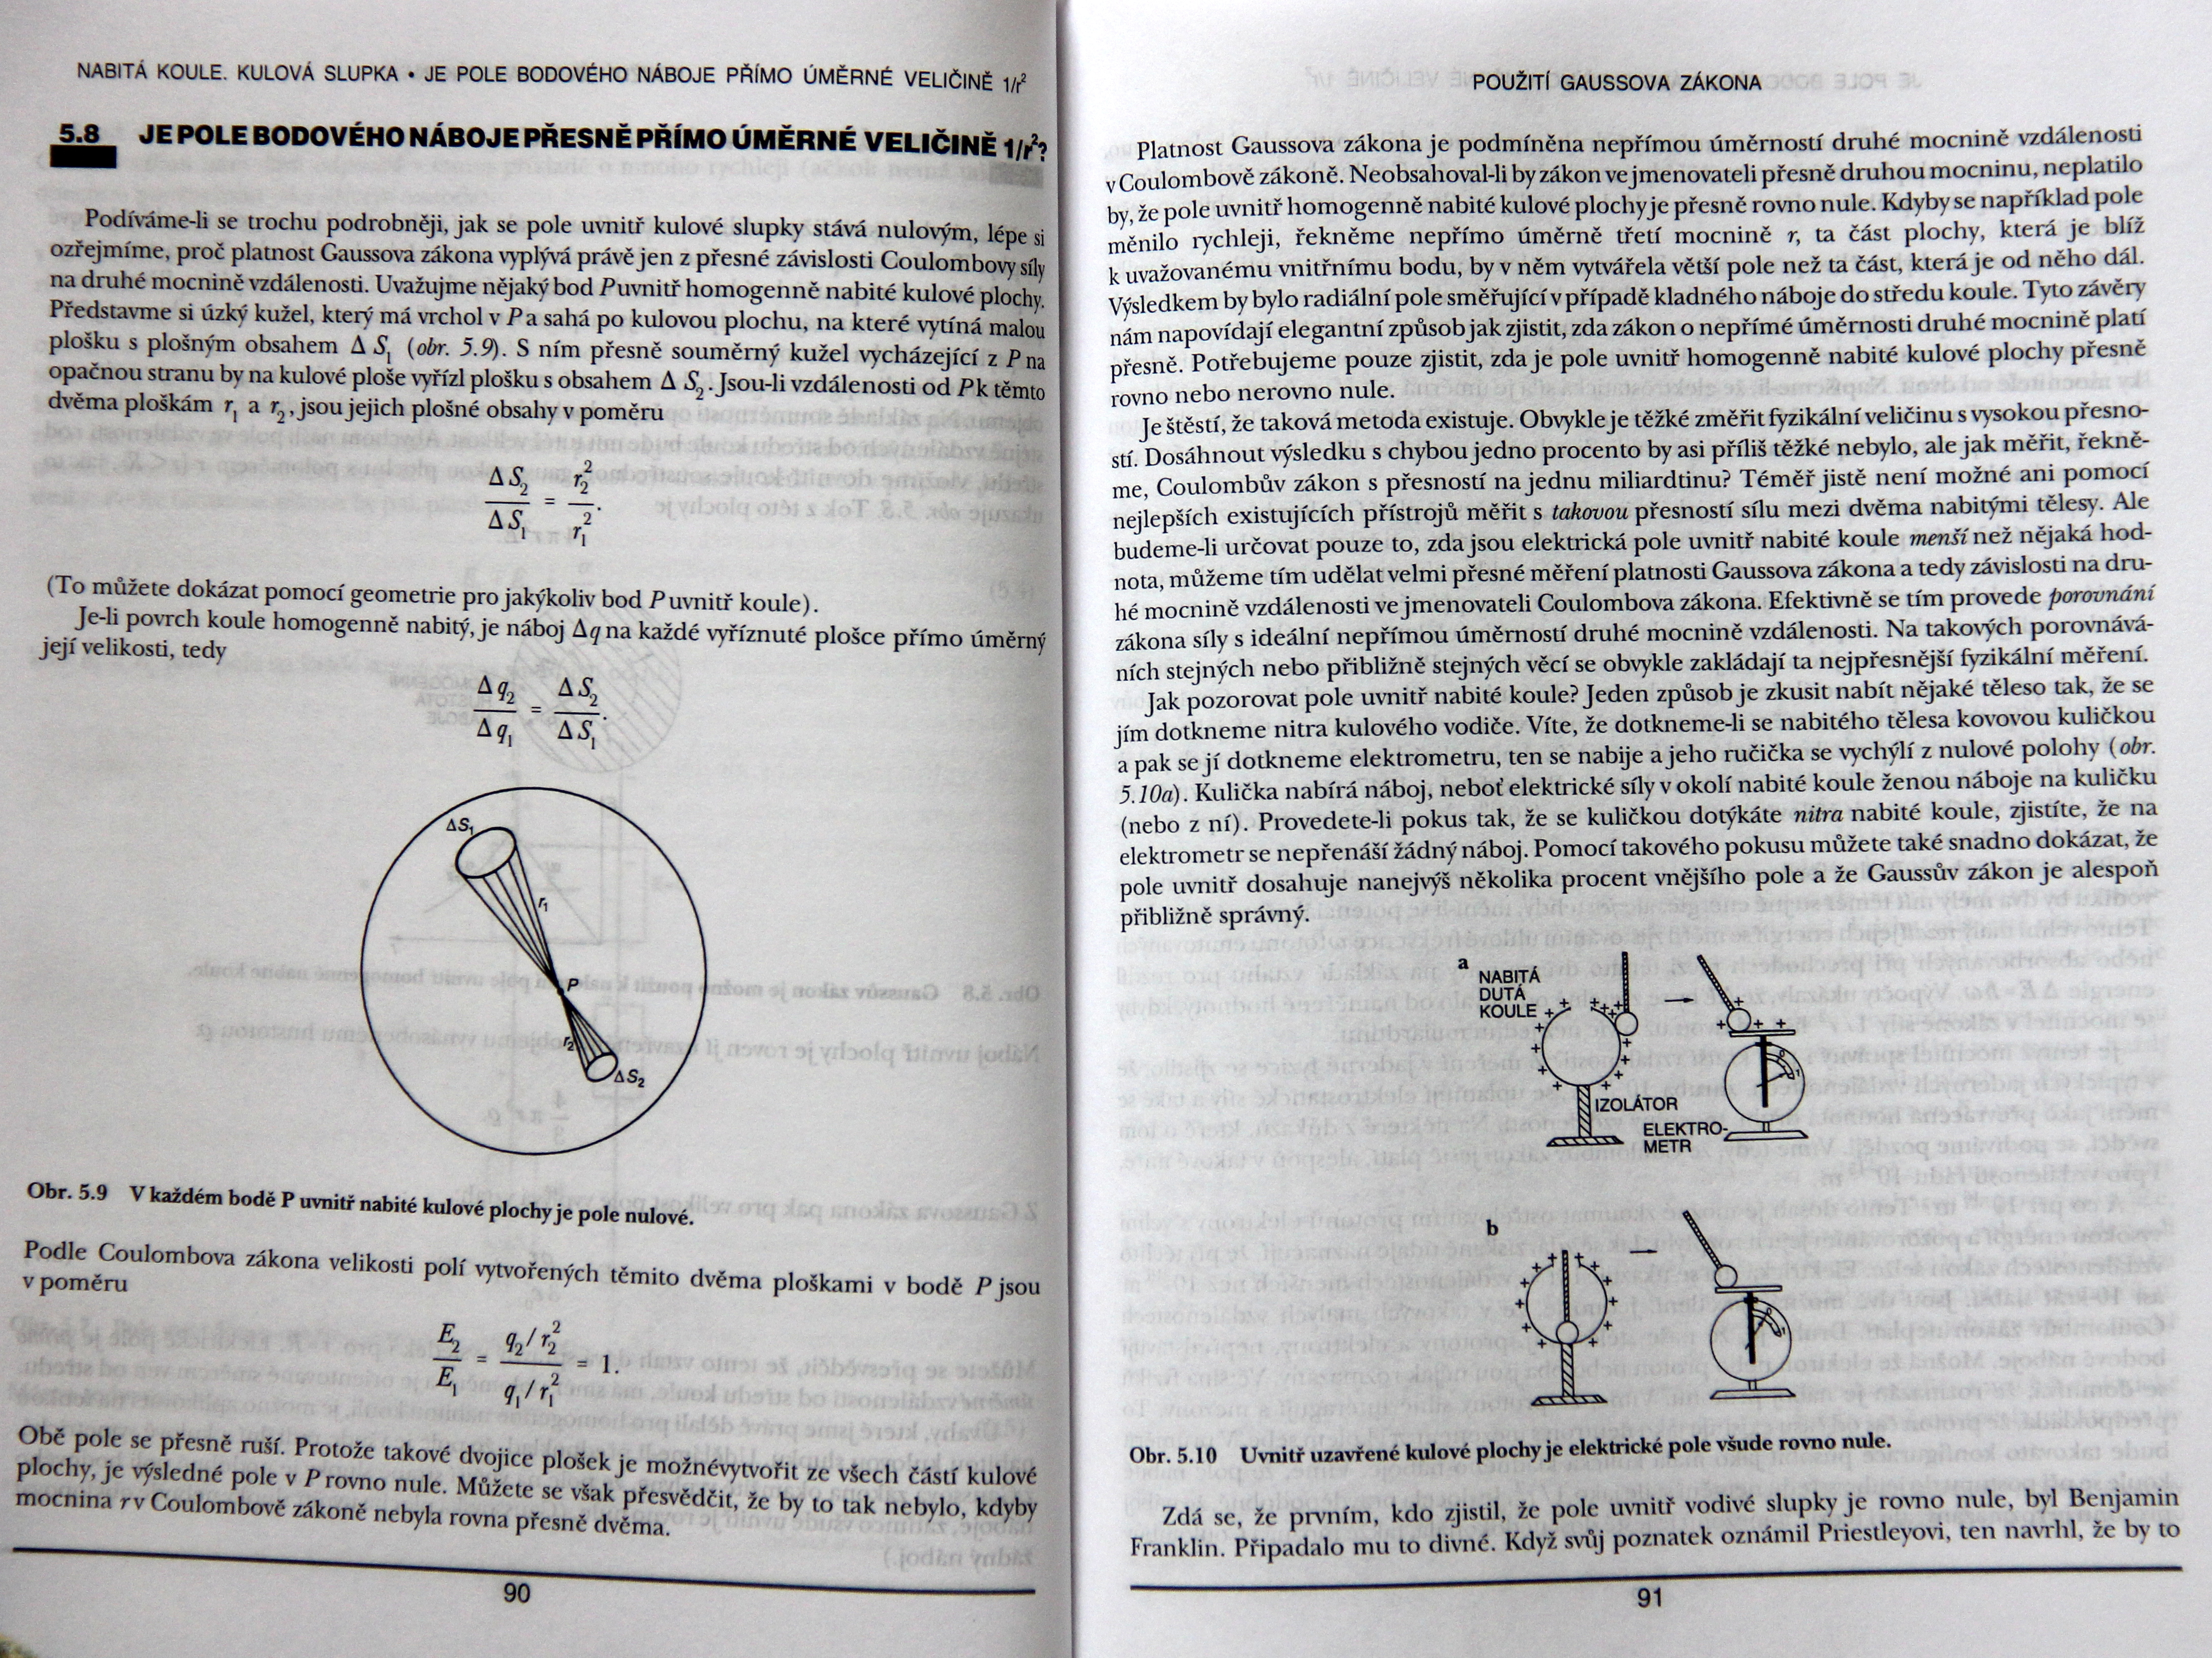
\includegraphics[width=0.6\linewidth]{fey_elstat_gauss09.jpg}
        \caption{V každém bodě \(P\) uvnitř nabité kulové plochy je pole nulové.}
        \label{fyz:fig_fey_elstat_gauss09}
      \end{figure}
      
      Podle Coulombova zákona velikosti polí vytvořených těmito dvěma ploškami v bodě \(P\) jsou v poměru
      \[\frac{E_2}{E_1} = \frac{q_2/r_2^2}{q_1/r_1^2} = 1.\]
      
      Obě pole se přesně ruší. Protože takové dvojice plošek je možné vytvořit že všech Částí kulové plochy, 
      je výsledné pole v \(P\) rovno nule. Můžeme se však přesvědčit, že by to tak nebylo, kdyby mocnina 
      \(r\) v Coulombově zákoně nebyla rovna přesně dvěma.
      
      Platnost Gaussova zákona je podmíněna nepřímou úměrností druhé mocnině vzdálenosti v Coulombově zákoně. 
      Neobsahoval-li by zákon ve jmenovateli přesně druhou mocninu, neplatilo by, že pole uvnitř homogenně 
      nabité kulové plochy je přesně rovno nule. Kdyby se například pole měnilo rychleji, řekněme nepřímo 
      úměrně třetí mocnině \(r\), ta část plochy, která je blíž k uvažovanému vnitřnímu bodu, by v něm 
      vytvářela větší pole než ta část, která je od něho dál. Výsledkem by bylo radiální pole směřující v 
      případě kladného náboje do středu koule. Tyto závěry nám napovídají elegantní způsob jak zjistit, zda 
      zákon o nepřímé úměrnosti druhé mocnině platí přesně. Potřebujeme pouze zjistit, zda je pole uvnitř 
      homogenně nabité kulové plochy přesně rovno nebo nerovno nule.
      
      Je štěstí, že taková metoda existuje. Obvykle je těžké změřit fyzikální veličinu s vysokou přesností. 
      Dosáhnout výsledku s chybou jedno procento by asi příliš těžké nebylo, ale jak měřit, řekněme, 
      Coulombův zákon s přesností na jednu miliardtinu? Téměř jistě není možné ani pomocí nejlepších 
      existujících přístrojů měřit s takovou přesností sílu mezi dvěma nabitými tělesy. Ale budeme-li určovat 
      pouze to, zda jsou elektrická pole uvnitř nabité koule menší než nějaká hodnota, můžeme tím udělat 
      velmi přesné měření platnosti Gaussova zákona a tedy závislosti na druhé mocnině vzdálenosti ve 
      jmenovateli Coulombova zákona. Efektivně se tím provede porovnání zákona síly s ideální nepřímou 
      úměrností druhé mocnině vzdálenosti. Na takových porovnáváních stejných nebo přibližně stejných věcí 
      se obvykle zakládají ta nejpřesnější fyzikální měření.
      
      Jak pozorovat pole uvnitř nabité koule? Jeden způsob je zkusit nabít nějaké těleso tak, že se jím 
      dotkneme nitra kulového vodiče. Víte, že dotkneme-li se nabitého tělesa kovovou kuličkou a pak sejí 
      dotkneme elektrometru, ten se nabije a jeho ručička se vychýlí z nulové polohy (obr 
      \ref{fyz:fig_fey_elstat_gauss10}). Kulička nabírá náboj, neboť elektrické síly v okolí nabité koule 
      ženou náboje na kuličku (nebo z ní). Provedeme-li pokus tak, že se kuličkou dotýkáte nitra nabité 
      koule, zjistíme, že na elektrometr se nepřenáší žádný náboj. Pomocí takového pokusu můžete také snadno 
      dokázat, že pole uvnitř dosahuje nanejvýš několika procent vnějšího pole a že Gaussův zákon je alespoň 
      přibližné správný \cite[s.~91]{Feynman02}.
      \begin{figure}[hb!]
        \centering
        \begin{tabular}{cc}
         \subfloat[ ]{\label{fyz:fig_fey_elstat_gauss10}
           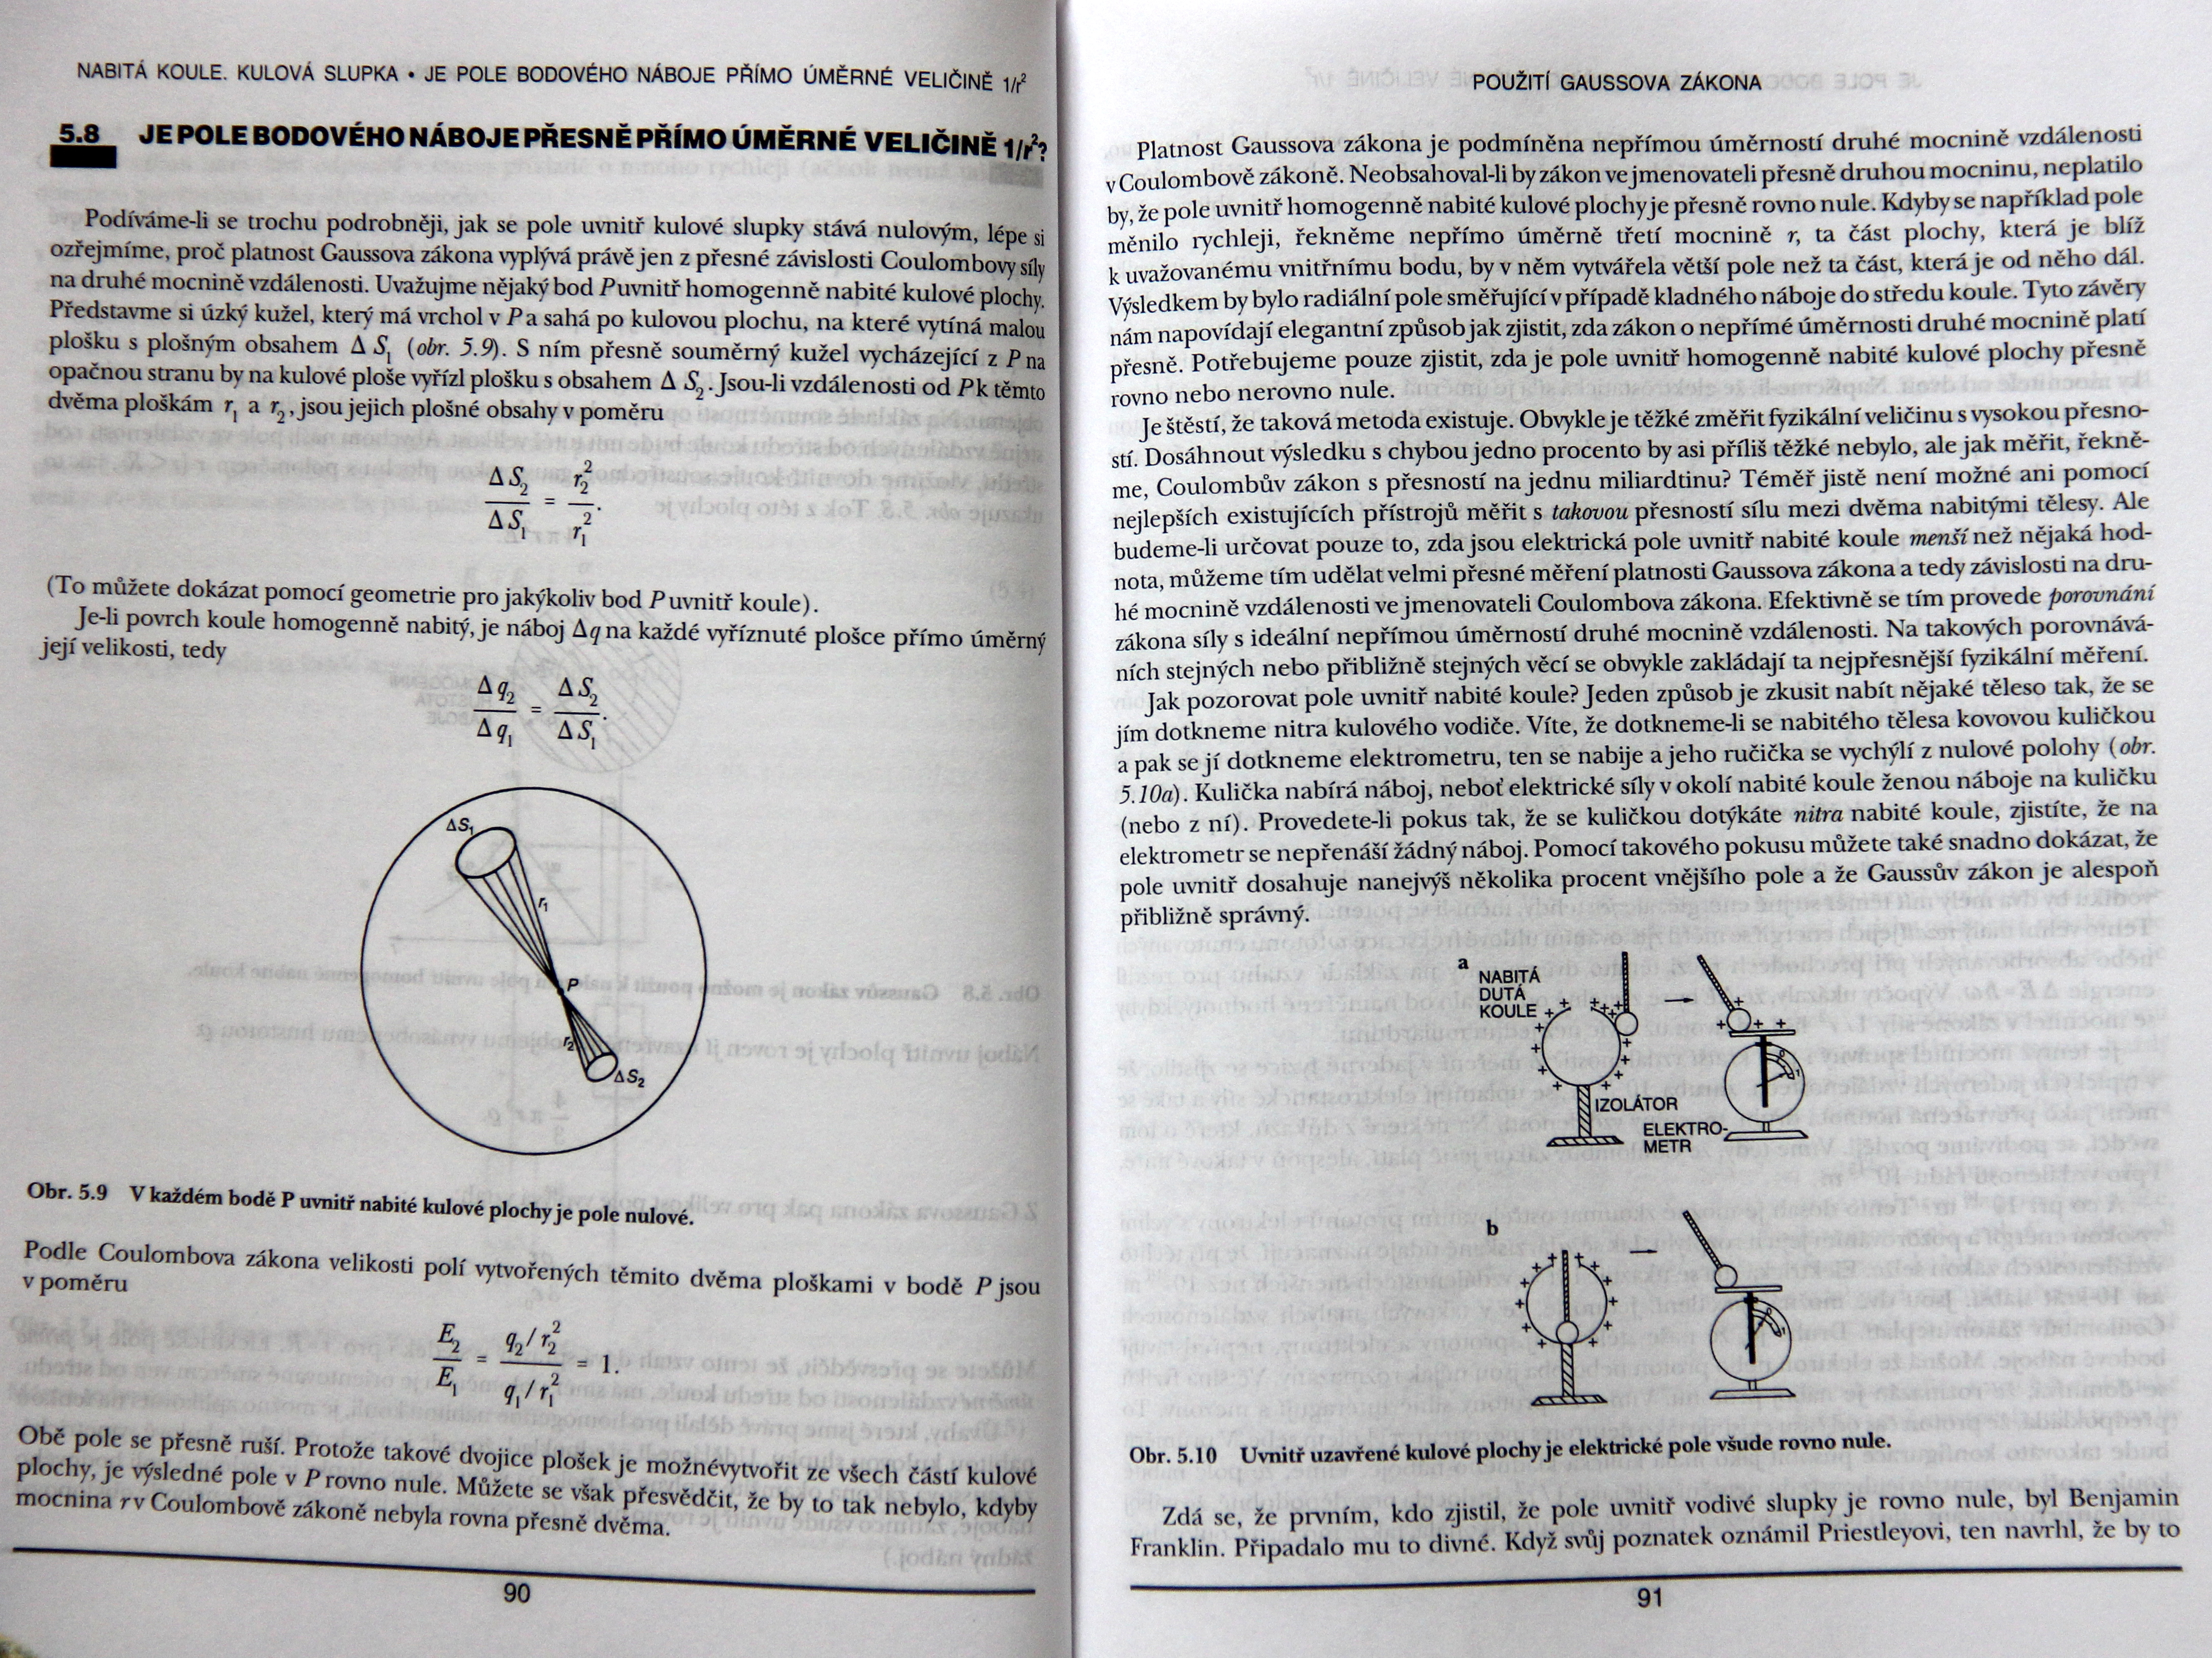
\includegraphics[width=0.2\textwidth]{fey_elstat_gauss10.jpg}}              &
         \subfloat[ ]{\label{fyz:fig_fey_elstat_gauss11}
           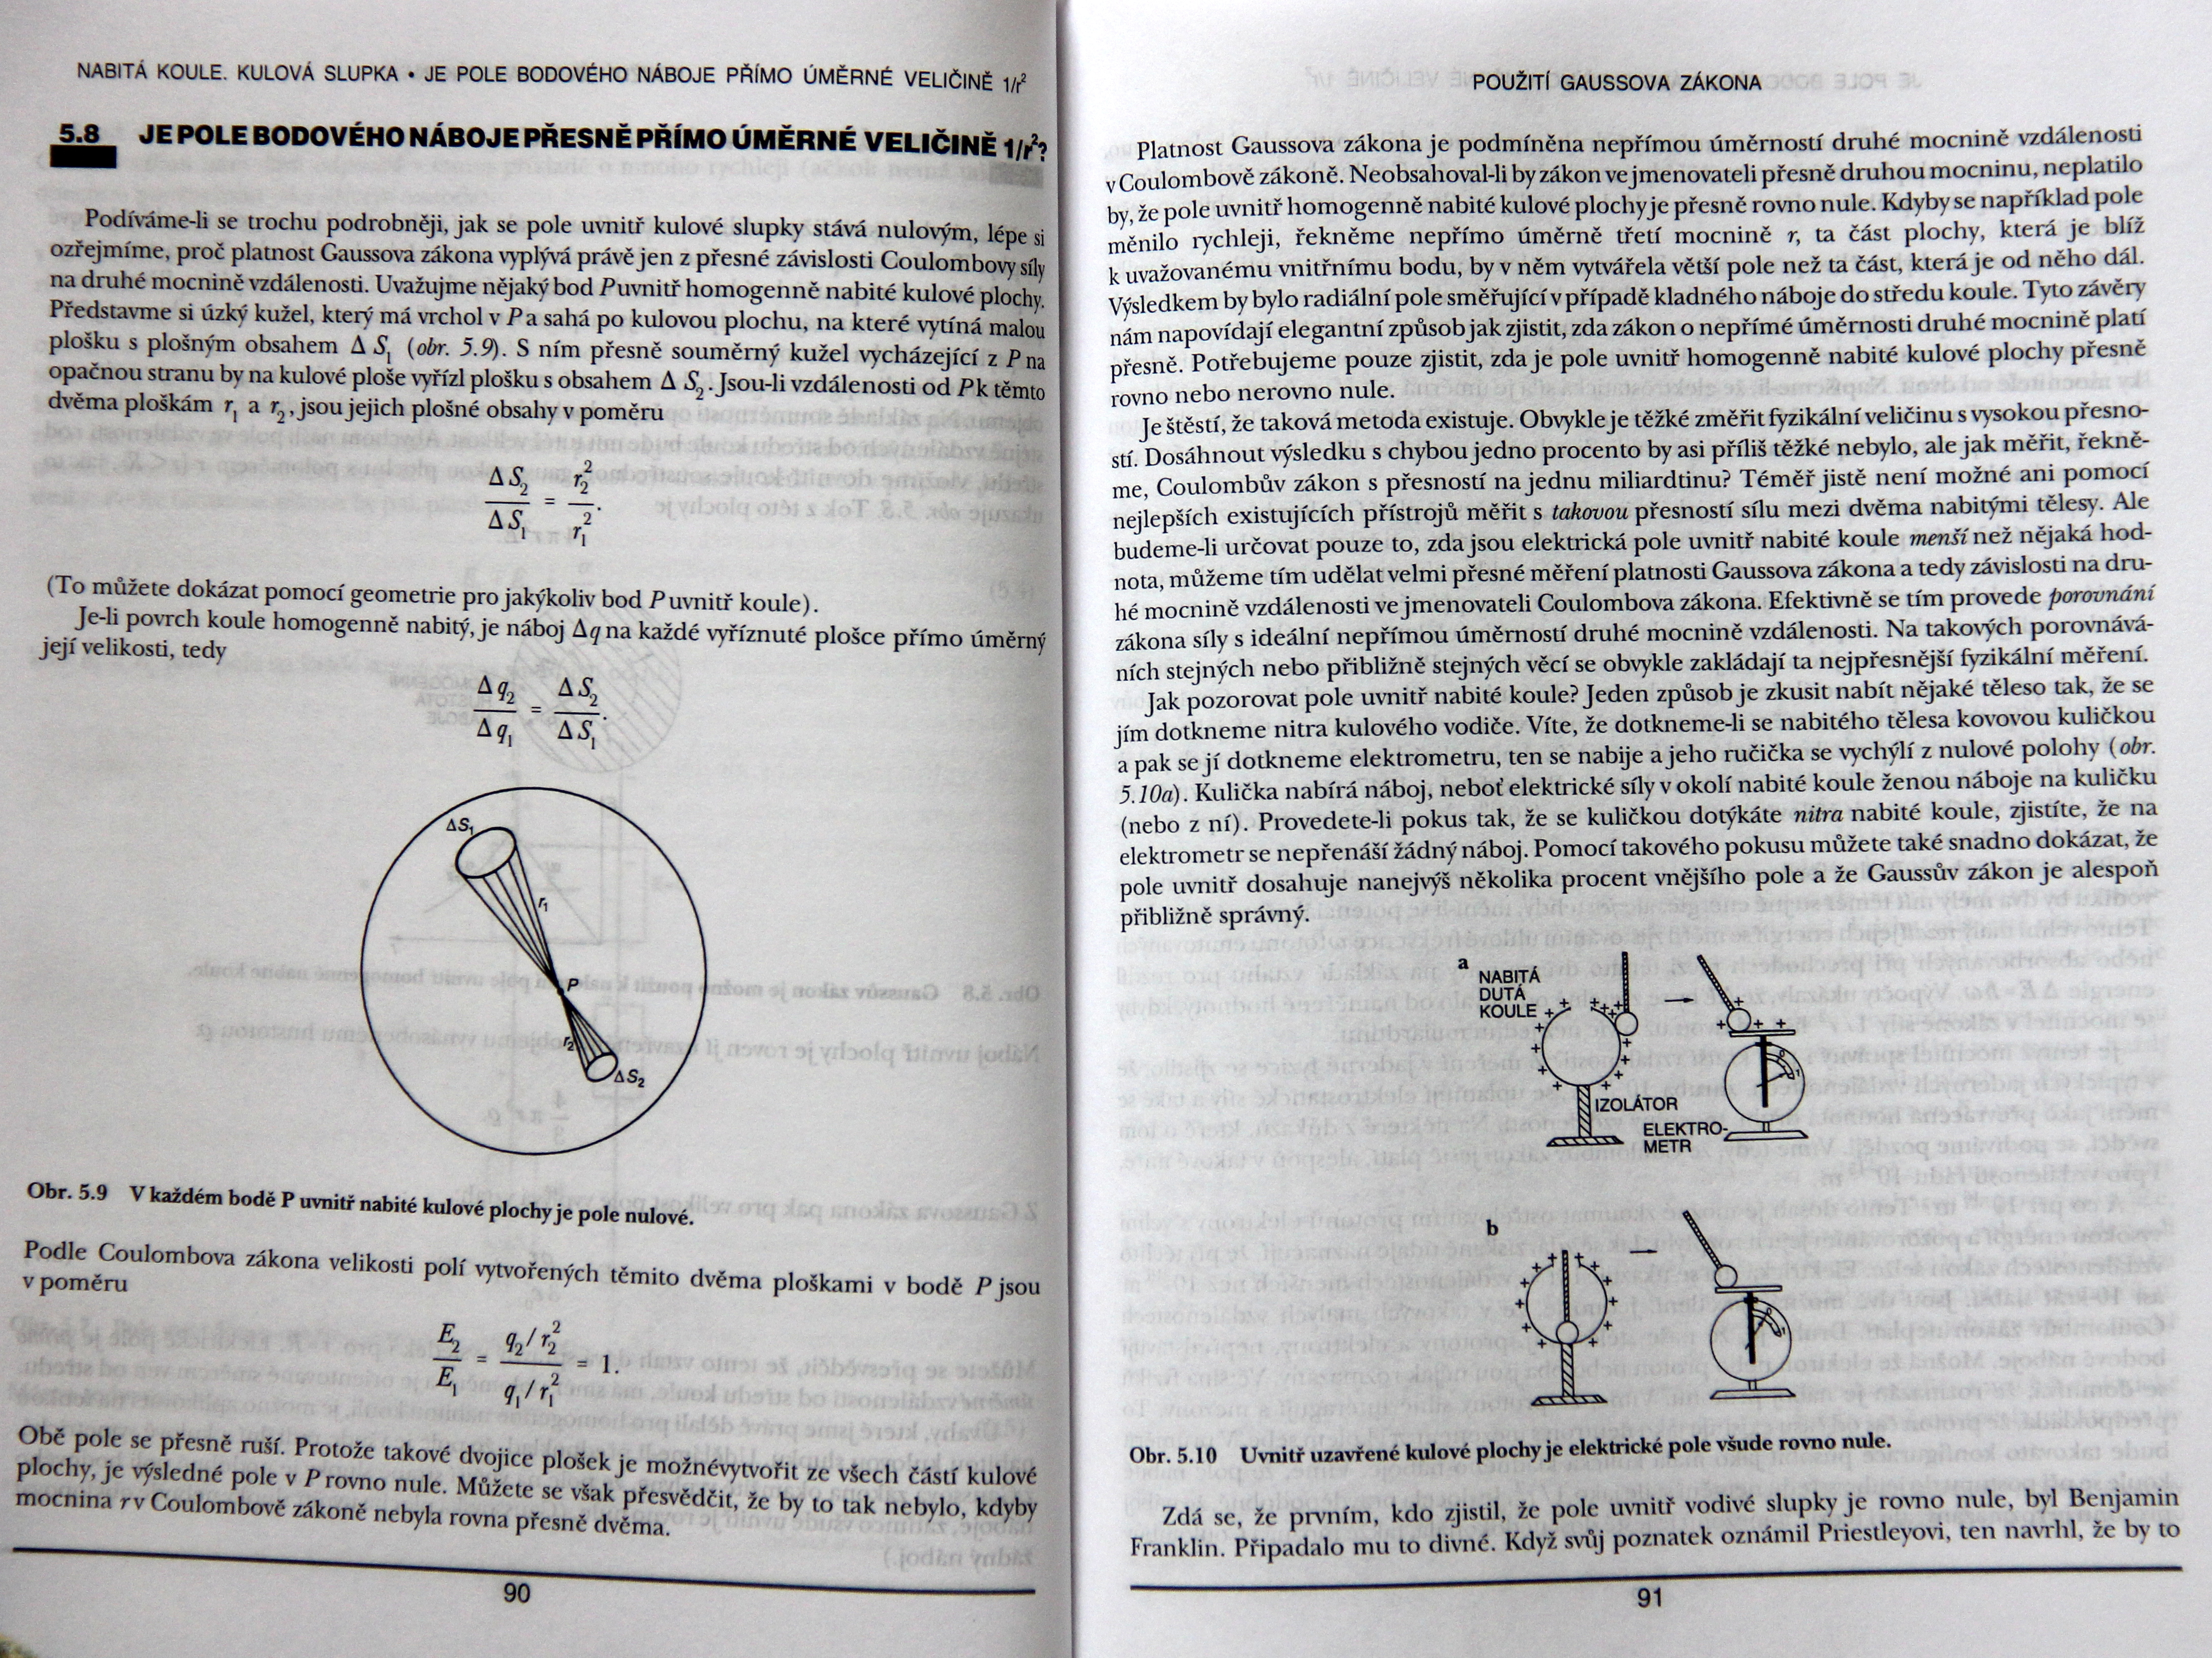
\includegraphics[width=0.2\textwidth]{fey_elstat_gauss11.jpg}}                        \\
        \end{tabular}                          
        \caption{Uvnitř uzavřené kulové plochy je elektrické pole všude rovno nule.}
        \label{fyz:fig_fey_elstat_gauss_koule}
      \end{figure}       
        
      Zdá se, že prvním, kdo zjistil, že pole uvnitř vodivé slupky je rovno nule, byl Benjamin Franklin. 
      Připadalo mu to divné. Když svůj poznatek oznámil Priestleyovi, ten navrhl, že mohlo souviset se 
      zákonem nepřímé úměrnosti druhé mocnině vzdálenosti, neboť bylo známo, že kulová hmotná slupka uvnitř 
      nevytváří žádné gravitační pole. Ale Coulomb naměřil nepřímou úměrnost druhé mocnině vzdálenosti až o 
      18 let později a Gaussův zákon byl objeven ještě později.
      
      Gaussův zákon byl pečlivě prověřován. Za tímto účelem se elektrometr umístil uvnitř velké koule a 
      sledovalo se, zda se neobjeví nějaké výchylky, když se koule nabije na vysoké napětí. Vždy bylo 
      dosaženo záporného výsledku. Z geometrie aparatury a citlivosti elektrometru je možné vypočítat, jaké 
      nejmenší pole by se projevilo. Z této hodnoty lze stanovit horní ohraničení odchylky mocnitele od dvou. 
      Napíšeme-li, že elektrostatická síla je úměrná \(r^{2+\varepsilon}\), můžeme určit horní hranici pro 
      \(\varepsilon\). Touto metodou Maxwell určil, že \(\varepsilon\) je méně než \(\num{1/10 000}\). V roce 
      1936 Plimpton a Laughton experiment zopakovali a zdokonalili. Zjistili, že mocnitel se liší od dvou o 
      méně než jednu miliardtinu.
      
      To nás přivádí k zajímavé otázce: Do jaké míry víme, jak přesně platí Coulombův zákon v různých 
      situacích? Právě popsané pokusy měří závislost pole na vzdálenosti řekněme několika desítek centimetrů. 
      Ale co třeba vzdálenosti uvnitř atomu, např. vodíkového atomu, v němž, jak předpokládáme, je elektron 
      přitahován k jádru podle téhož zákona nepřímé úměrnosti druhé mocnině vzdálenosti? Je pravda, že k 
      popisu mechanické stránky chování elektronu musí být použita kvantová mechanika, ale přitom jde o 
      obyčejnou elektrostatickou sílu. Při formulování úlohy o atomu vodíku je potřeba znát potenciální 
      energii elektronu jako funkci vzdálenosti od jádra. Coulombův zákon dává potenciál, který se mění 
      nepřímo úměrně první mocnině vzdálenosti. S jakou přesností je znám mocnitel pro takové malé 
      vzdálenosti? Z velmi pečlivých měření relativních poloh energetických hladin vodíku, které provedli 
      Lamb a Retherford r. 1947, víme, že v rozměrech atomu, tj. ve vzdálenostech řádově desetin nanometru 
      (\SI{10e-10}{\meter}), Souhlasí mocnitel opět s přesností jedné miliardtiny.
      
      Přesnost Lambova-Retherfordova měření znovu umožnila fyzikální „náhoda“. Ze stavů atomu vodíku by dva 
      měly mít téměř stejné energie, ale jen tehdy, mění-li se potenciál přesně jako \(1/r\). Tento velmi 
      malý rozdíl jejich energií se měřil zjišťováním úhlové frekvence \(\omega\) fotonů emitovaných nebo 
      absorbovaných při přechodech mezi těmito dvěma stavy na základě vztahu pro rozdíl energie \(\Delta E 
      = \si{\planckbar}\omega\)). Výpočty ukázaly, že \(\delta E\) by se zřetelně odlišovalo od naměřené 
      hodnoty, kdyby se mocnitel v zákoně síly \(1/r^2\) lišil od dvou už o víc než jednu miliardtinu.
      
      Je tentýž mocnitel správný i pro kratší vzdálenosti? Z měření v jaderné fyzice se zjistilo, že v 
      typických jaderných vzdálenostech, zhruba \SI{10e-15}{\meter}, se uplatňují elektrostatické síly a také 
      se mění jako převrácená hodnota druhé mocniny vzdálenosti. Na některé z důkazů, které o tom svědčí, se 
      podíváme později. Víme tedy, že Coulombův zákon ještě platí, alespoň v takové míře, i pro vzdálenosti 
      řádu \SI{10e-10}{\meter}.
      
      A co při \SI{10e-16}{\meter}? Tento dosah je možné zkoumat ostřelováním protonů elektrony s velmi 
      vysokou energií a pozorováním jejich rozptylu. Jak se zdá, získané údaje naznačují, že při těchto 
      vzdálenostech zákon selže. Elektrická síla se ukazuje být ve vzdálenostech menších než 
      \SI{10e-16}{\meter} asi 10-krát slabší. Jsou dvě možná vysvětlení. Jedno je, že v takových malých 
      vzdálenostech Coulombův zákon neplatí. Druhé je, že naše „tělesa“, tj. protony a elektrony, 
      nepředstavují bodové náboje. Možná že elektron nebo proton nebo oba jsou nějak rozmazány. Většina 
      fyziků se domnívá, že rozmazán je náboj protonu. Víme, že protony silně interagují s mezony. To 
      předpokládá, že proton čas od času existuje jako neutron s mezonem \(\pi^+\) kolem sebe. V průměru bude 
      takováto konfigurace působit jako malá kulička kladného náboje. Víme, že pole nabité koule se při 
      postupu do jejího středu nemění stále jako \(1/r^2\). Je docela pravděpodobné, že náboj protonu je 
      rozmazaný, ale i teorie \(\pi\text{-mezonů}\) je ještě dost nedokonalá, takže možná i Coulombův zákon 
      selže na velmi malých vzdálenostech\footnote{Experimenty, které Feynman popisuje, postupně vedly k 
      dnešní představě, podle níž protony, neutrony i mezony skutečně nejsou bodové částice, ale mají vnitřní 
      strukturu tvořenou kvarky. Kvarky přitom nemohou existovat samostatně.}.
      
      Ještě jedna věc: zákon nepřímé úměrnosti druhé mocnině vzdáleností platí pro vzdálenosti řádu 
      \SI{1}{\meter}, ale i pro \SI{10e-10}{\meter}; zůstává však činitel \(\dfrac{1}{4\pi\varepsilon_0}\) 
      stále stejným? Odpověď je ano, alespoň s relativní přesností 15 milióntin.
      
      Nyní se vraťme k důležitému problému, který jsme přešli mlčením, když jsme hovořili o experimentálním 
      potvrzení Gaussova zákona. Možná, že jste se podivili, jak mohl být výsledek experimentu Maxwella nebo 
      Plimptona a Lauglitona tak přesný, když přitom kulový vodič, který použili, nebyl dokonalou koulí. 
      Vždyť dosáhnout přesnosti na jednu miliardtinu je už opravdu něco a právem byste se mohli ptát, zda 
      dokázali udělat tak přesnou kouli. Každá reálná koule má určitě malé nepravidelností. Existují-li 
      nepravidelnosti, nebudou uvnitř vytvářet pole? Nyní chceme ukázat, že není třeba mít dokonalou kouli. 
      Opravdu lze dokázat, že uvnitř uzavřené vodivé plochy jakéhokoliv tvaru není žádné pole. Jinými slovy, 
      výsledek zmíněných experimentů závisel na \(1/r^2\), ale vůbec ne na tom, zda je plocha kulová (až na 
      to, že pro kouli je snazší vypočítat, jaká by byla pole, kdyby Coulombův zákon neplatil), a tak se nyní 
      vracíme znovu k našemu problému. Abychom to ukázali, je nevyhnutelné poznat některé vlastností 
      elektrických vodičů.
      
    \subsection{Pole vodiče}
      Elektrickým vodičem je pevné těleso, které obsahuje mnoho „volných“ elektronů. Elektrony se mohou v 
      tělese volně pohybovat, ale nemohou projít jeho povrchem. V kovu je tolik volných elektronů, že 
      jakékoliv elektrické pole jich uvede do pohybu velké množství. Takto vzniklý proud elektronů se pak 
      musí buď udržovat vnějšími zdroji energie, nebo se pohyb elektronů zastaví, jakmile elektrony vybijí 
      zdroje, které vytvořily původní pole. V elektrostatice nepracujeme se stálými zdroji proudu (jimi se 
      budeme zabývat později, až budeme hovořit o magnetostatice), takže elektrony se pohybují jen dokud se 
      neuspořádají tak, aby všude uvnitř vodiče vytvořily nulové elektrické pole. (Obvykle se to stane v 
      malém zlomku sekundy). Kdyby totiž ještě nějaké pole zůstalo, uvedlo by do pohybu další elektrony; 
      jediným možným řešením v elektrostatice je, že je pole uvnitř vodiče je všude nulové.
      
      Nyní si všimněme vnitřku nabitého vodivého tělesa. („Vnitřkem“ rozumíme prostor v objemu kovu.) Protože 
      kov je vodič, vnitřní pole, a tedy gradient potenciálu \(\varphi\) musí být roven nule. Každý vodič tak 
      představuje ekvipotenciální oblast a jeho povrch je ekvipotenciální plochou. Protože všude ve vodivé 
      látce je elektrické pole rovno nule, je nule rovna i divergence \(\vec{E}\) a podle Gaussova zákona 
      musí být rovna nule i hustota náboje uvnitř vodiče.
      
      Nemohou-li být ve vodiči žádné náboje, jak je možné jej nabít? Co máme na mysli, když říkáme, že je 
      vodič „nabit“? Kde tedy náboje jsou? Odpověď je, že se nacházejí na povrchu vodiče, kde působí velké 
      síly, které jim zabraňují uniknout, tedy náboje nejsou zcela „volné“. Budeme-li studovat fyziku pevných 
      látek, dozvíme se, že přebytečný náboj se v každém vodiči nachází v jedné - dvou atomových vrstvách 
      povrchu. Pro naše současné účely je dostačující přesnost říkat, že převede-li se nějaký náboj na vodič 
      nebo do něj, celý se shromáždí na jeho povrchu; uvnitř vodiče žádné náboje nejsou.
      
      Kromě toho si všimněte, že na vnější straně v těsné blízkosti povrchu vodiče musí být elektrické pole 
      kolmé na povrch. Nemůže existovat žádná tečná složka. Kdyby totiž existovala, elektrony by se 
      pohybovaly podél povrchu; neexistují žádné síly, které by jim v tom zabraňovaly. Jinými slovy víme, že 
      elektrické siločáry musí vždy svírat s ekvipotenciální plochou pravý úhel.
      
      Na základě Gaussova zákona můžeme také uvést do vztahu intenzitu pole blízko povrchu vodiče s lokální 
      hustotou náboje na jeho povrchu. Jako gaussovskou plochu vezmeme malou válcovou krabičku jednou 
      polovičkou pod a druhou polovičkou nad povrchem (obr. \ref{fyz:fig_fey_elstat_gauss12}). K celkovému 
      toku \(\vec{E}\) přispívá pouze ta strana krabičky, která je mimo vodič. Pole těsně při povrchu vodiče 
      z jeho vnější strany je potom
      \begin{figure}[ht!] % \ref{fyz:fig_fey_elstat_gauss12}
        \centering
        \includegraphics[width=0.4\linewidth]{fey_elstat_gauss12.png}
        \caption{Elektrické pole těsně při povrchu vodiče je přímo úměrné lokální plošné hustotě náboje na 
                 povrchu.}
        \label{fyz:fig_fey_elstat_gauss12}
      \end{figure} 
      Vně vodiče
      \begin{equation}\label{fyz:eq_fey_elstat_gauss07}
        E = \frac{\sigma}{\varepsilon_0}  \qquad\text{\(\sigma\ldots\) lokální plošná hustota náboje}.
      \end{equation}
      
      Proč nabitá vrstva na povrchu náboje vytváří jiné pole než samotná nabitá rovina? Jinými slovy, proč je 
      (\ref{fyz:eq_fey_elstat_gauss07}) dvakrát větší než (\ref{fyz:eq_fey_elstat_gauss03})? Důvod spočívá, 
      samozřejmě, v tom, že v případě vodiče jsme netvrdili, že se v okolí nenacházejí žádné „jiné“ náboje. 
      Opravdu nějaké ještě musí být, aby ve vodiči bylo \(\vec{E} = 0\). Náboje, nacházející se v 
      bezprostředním sousedství bodu \(P\) na povrchu vodiče, ve skutečnosti vytvářejí pole 
      \(E_{lok}=\frac{\sigma_{lok}}{2\varepsilon_0}\) jak z vnitřní tak i z vnější strany povrchu. Ale všechny
      ostatní náboje na vodiči se „spikly“, aby vytvořily v bodě \(P\) dodatkové pole s velikostí 
      \(E_{lok}\). Výsledné vnitřní pole je pak nulové a vnější je rovno \(2E_{lok} = 
      \frac{\sigma_{lok}}{\varepsilon_0}\) \cite[s.~93]{Feynman02}.
      
    \subsection{Pole vodiče}
      Nyní se vrátíme k problému duté schránky - vodiči s dutinou. Uvnitř kovu není žádné pole, ale jak tomu 
      bude v dutině? Ukážeme, že je-li dutina prázdná, pak v ní pole nejsou bez ohledu na to, jaký tvar má 
      vodič nebo dutina. Ukážeme to například pro tvar na obr. \ref{fyz:fig_fey_elstat_gauss13}. Uvažujme 
      gaussovskou plochu takového tvaru, jaký má plocha \(S\) vyznačená na obr. 
      \ref{fyz:fig_fey_elstat_gauss13}, která obklopuje dutinu, ale všude zůstává ve vodivé látce. Všude na 
      \(S\) je pole rovno nule, takže není žádný tok z \(S\) a celkový náboj uvnitř \(S\) je roven nule. 
      Kdyby šlo o kulovou plochu, by bylo možno ze souměrnosti usoudit, že v jejím nitru by nemohl být žádný 
      náboj. Ale obecně můžeme pouze tvrdit, že na vnitřním povrchu vodiče je stejné množství kladného a 
      záporného náboje. Kladný povrchový náboj by mohl být v jedné jeho části a záporný někde jinde, jako na 
      obr. \ref{fyz:fig_fey_elstat_gauss13}. Gaussovým zákonem není možné něco takového vyloučit.
      \begin{figure}[ht!] % \ref{fyz:fig_fey_elstat_gauss13}
        \centering
        \includegraphics[width=0.4\linewidth]{fey_elstat_gauss13.png}
        \caption{Jaké pole je v prázdné dutině ve vodiči při jakémkoliv tvaru vodiče a dutiny?}
        \label{fyz:fig_fey_elstat_gauss13}
      \end{figure} 
      
      Ve skutečnosti však jakékoliv stejně velké a opačné náboje, nacházející se na vnitřním povrchu, k sobě 
      sklouznou a úplně se vyruší. To, že musí být vyrušeny úplně, můžeme ukázat použitím zákona, že 
      cirkulace pole \(\vec{E}\) je vždy rovna nule (v elektrostatice). Předpokládejme, že by se v některých 
      částech vnitřního povrchu nacházely náboje. Víme, že někde jinde na povrchu by se muselo nacházet 
      stejné množství opačných nábojů. Jakékoliv siločáry pole \(\vec{E}\) by nyní musely vycházet z kladných 
      nábojů a končit v záporných nábojích (neboť uvažujeme pouze o případě, že v dutině nejsou volné 
      náboje). Představme si nyní uzavřenou křivku \(\Gamma\), která prochází napříč dutinou podél některé 
      siločáry od nějakého kladného k některému zápornému náboji a vodičem se vrací zpět do svého výchozího 
      bodu. (jako na obr. \ref{fyz:fig_fey_elstat_gauss13}). Integrál po takové siločáře vedoucí od kladného 
      k zápornému náboji nebude roven nule. Integrál po křivce uvnitř kovu dá však nulu, neboť \(\vec{E}=0\). 
      Dostali jsme tedy že
      \begin{equation}\label{fyz:eq_fey_elstat_gauss08}
        \oint \vec{E}\cdot\dd{\vec{S}} \neq 0  \qquad ???
      \end{equation}
      Křivkový integrál pole \(\vec{E}\) po každé uzavřené křivce je však v elektrostatickém poli roven nule. 
      Z toho vyplývá, že uvnitř prázdné dutiny nemohou existovat žádná pole ani žádné náboje na jejím povrchu.
      
      Měli bychom si pečlivě všimnout důležité výhrady, kterou jsme uvedli. Vždy jsme říkali „uvnitř prázdné“ 
      dutiny. Umístí-li se totiž nějaké náboje do některých pevných poloh v dutině, ať už v izolantu, nebo na 
      malém vodiči izolovaném od hlavního vodivého tělesa, pak se v dutině mohou objevit pole. Ale pak už to 
      není „prázdná“ dutina.
      
      Ukázali jsme, že je-li dutina úplně obklopena vodičem, žádné statické rozdělení nábojů mimo ni nikdy 
      nemůže vytvořit pole v jejím nitru. Tím se vysvětluje princip „stínění“ elektrického zařízení, které 
      je uloženo v kovovém obalu. Stejné úvahy můžeme použít i v důkazu, že žádné statické rozdělení nábojů 
      uvnitř uzavřeného vodiče nemůže vytvořit nějaká pole ve vnějším prostoru. Stínění funguje v obou 
      směrech. V elektrostatice - ne však při proměnných polích - pole na obou stranách uzavřené vodivé 
      plochy jsou úplně nezávislá.
      
      \emph{Nyní chápeme, proč bylo možné prověřit Coulombův zákon s tak velkou přesností. Tvar duté schránky 
      je bezvýznamný. Nemusí být kulový, mohla by to být krychle. Je-li Gaussův zákon přesný, je pole uvnitř 
      vždy nulové. Teď také chápeme, proč je bezpečné sedět uvnitř vysokonapěťové elektrody megavoltového van 
      de Graaffova generátoru bez obavy ze zásahu elektřinou. Umožňuje to Gaussův zákon.}

  %--------------------------------- Elektrické pole v různých případech -------------------------------------
  \section{Elektrické pole v různých případech} 
  
\printbibliography[heading=subbibliography]   
%=====================================Kapitola: Speciální teorie relativity========================= 
  %==============================Kapitola: Speciální teorie relativity=================================
\chapter{Speciální teorie relativity}
\minitoc
\newpage
  \section{Princip relativity}
    Více než 200 let se věřilo, že Newtonovy ronice správně popisují přírodu. Když se v nich poprvé 
    našla chyba, našel se i způsob, jak jej odstranit. Oboje, chybu i korekci, objevil Einstein v 
    roce 1905.
    
    V druhém Newtonově zákoně, daném vztahem $$\vr{F} = \der{(mv)}{t}$$ se mlčky předpokládalo, že 
    $m$ je konstantní veličina. Ale nyní víme, že to není pravda a že hmotnost tělesa roste, 
    zvyšuje-li se jeho rychlost. V Einsteinově opraveném vztahu má $m$ hodnotu 
    \begin{equation}\label{TEMP:eq_fey_rel_01}
      m = \frac{m_0}{\sqrt{1-\frac{v^2}{c^2}}}
    \end{equation}  
    kde $m_0$ je \emph{klidová hmotnost} (hmotnost tělesa, jež se nepohybuje) a $c$ je 
    \emph{rychlost světla}, která je přibližně rovna $3\cdot10^5\,
    km\cdot s^{-1}$.
    
    Ze vztahu je vidět, že za normálních okolností je přírůstek hmotnosti velmi malý. Dokonce i pro 
    družici Země, jež se pohybuje rychlostí $9,0\, km\cdot s^{-1}$ je $v/c = 3\cdot10^{-5}$ a po 
    dosazení do uvedeného vztahu dostaneme korekci hmotnosti ne větší než dvě až tři miliardtiny, 
    což téměř nelze pozorovat. Platnost vztahu však byla dostatečně potvrzena pozorováním mnoha 
    druhů částic, jejichž rychlosti dosahují prakticky až rychlosti světla. Za normálních okolností 
    je tento efekt velmi malý a proto je pozoruhodné, že byl objeven nejprve teoreticky a až potom 
    experimentálně. Proto je zajímavé sledovat, jaké kombinace experimentů a fyzikálních úvah vedla 
    k odhalení tak jemné modifikace zákona. Přispělo k tomu nemálo lidí, přičemž konečným výsledkem 
    byl Einsteinův objev.
    
    Existují dvě Einsteinovy teorie relativity. Tato kapitola hovoří o \emph{speciální teorii 
    relativity} z roku 1905. V roce 1915 uveřejnil Einstein dodatečnou teorii nazvanou \emph{Obecná 
    teorie relativity}. Ta je zobecněním speciální teorie relativity pro případ \emph{gravitace}.
         
    Newton byl první, kdo vyslovil \emph{princip relativity} jako jeden z důsledků pohybových 
    zákonů: Vzájemné pohyby těles, nacházejících se v daném prostoru, jsou stejné ať je prostor v 
    klidu, nebo se pohybuje rovnoměrně přímočaře vpřed. To například znamená, že jestliže se 
    kosmická loď pohybuje rovnoměrnou rychlostí, všechny experimenty a všechny jevy v lodi budou 
    probíhat tak, jakoby se loď nepohybovala (samozřejmě za předpokladu, že se nikdo nebude dívat 
    ven). To je smyslem principu relativity. Myšlenka je jednoduchá, jedinou otázkou je, zda je 
    pravda, že ve všech experimentech provedených v pohybující se soustavě budou všechny fyzikální 
    zákony stejné, jako v soustavě, která je v klidu. Nejprve zjistíme, zda v pohybující se soustavě 
    mají Newtonovy zákony stejný tvar.        
    
    \begin{figure}
      \centering
      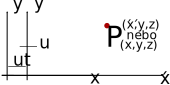
\includegraphics[width=0.8\linewidth]{fey_princip_relativity.pdf}
      \caption{Dvě souřadnicové soustavy v rovnoměrném relativním pohybu podél svých x-ových os.}
      \label{fyz:fig_fey_spec_relativita}
    \end{figure}
    
    Předpokládejme, že se Pavel pohybuje konstantní rychlostí $u$ ve směru osy $x$, přičemž měří 
    polohu určitého budu (obr. \ref{fyz:fig_fey_spec_relativita}). Ve své souřadnicové soustavě si 
    značí souřadnici ve směru osy $x$ jako $x'$. Petr je v klidu, přičemž měří polohu téhož bodu. 
    Souřadnici ve směru osy $x$ ve své souřadnicové soustavě značí jako $x$. Počátek souřadnicové 
    soustavy, v níž je Pavel, se posunu za čas $t$ o vzdálenost $ut$, a jestliže soustavy z počátku 
    splývaly, máme
    \begin{equation}\label{TEMP:eq_fey_rel_02}
      x' = x - ut, \qquad y' = y, \qquad z' = z, \qquad t' = t. 
    \end{equation}      
    Dosadíme-li tuto transformaci do Newtonových zákonů, zjistíme, že se přetransformovaly do 
    stejných zákonů v čárkované soustavě. To znamená, že Newtonovy zákony mají stejný tvar v 
    pohybující se soustavě jako v stacionární soustavě, a proto na základě mechanických experimentů 
    není možné říci, zda se soustava pohybuje či nikoliv. 
    
    Zájem o tento princip vzrostl v minulém století v důsledku výzkumu elektrických, magnetických a 
    světelných jevů, jež vyústilo v \emph{Maxwellovu teorii elektromagnetického pole}, která 
    jednotně popisuje elektřinu, magnetizmus a světlo. Zdálo se však, že Maxwellovy rovnice 
    nevyhovovaly \emph{principu relativity}, neboť přetransformujeme-li Maxwellovy rovnice pomocí 
    rovnic \ref{TEMP:eq_fey_rel_02}, nebudou mít stejný tvar. Proto by se elektrické a optické jevy 
    v letící kosmické lodi měli lišit od jevů v nehybné lodi. Těmito jevy by pak bylo možné určit 
    rychlost lodi, a ve speciálním případě pomocí vhodných optických nebo elektrických měření by 
    bylo možné určit i absolutní rychlost lodi. Jedním z důsledků Maxwellových rovnic je, že 
    dojde-li k určité poruše pole, při níž vniká světlo, toto elektromagnetické vlnění se šíří všemi 
    směry stejnou rychlostí $c = 3\cdot10^5\,km\cdot s^{-1}$. Dalším důsledkem těchto rovnic je, že 
    pohybuje-li se zdroj poruchy, šíří se vyzářené světlo prostorem stejnou rychlostí $c$. Tato 
    nezávislost pohybu vlnění na pohybu zdroje vede k zajímavému problému:
    
    Předpokládejme, že sedíme v autě, jež jede rychlostí $u$ a že světlo z reflektorů auta za námi 
    nás míjí rychlostí $c$. Zdiferencováním první rovnice \ref{TEMP:eq_fey_rel_02} máme
    \begin{equation}\label{TEMP:eq_fey_rel_03}
      \der{x'}{t} =\der{x}{t} - u, 
    \end{equation}       
    což znamená, že podle \emph{Galileovy transformace} by zdánlivá rychlost světla měřená z auta 
    nemohla být $c$, ale $c-u$. Na této myšlence bylo založeno mnoho experimentů k určení rychlosti 
    Země, ale všechny selhaly - nedávaly vůbec žádné rychlosti. Ukázalo se, že někde byla chyba, a 
    sice něco nebylo v pořádku s fyzikálními rovnicemi. Co to asi mohlo být?

  %------------------------ Lorentzova transformace -------------------------------------------------
  \section{Lorentzova transformace}
    Když se zjistilo, že s rovnicemi v uvedeném případě není vše v pořádku, nejprve padlo podezření 
    na Maxwellovy rovnice elektrodynamiky, jež byly tehdy známy jen dvacet let. Zdálo se být téměř 
    samozřejmé, že tyto rovnice musí byt nesprávné a proto byla snaha je změnit tak, aby při 
    Galileiho transformaci zachovávaly princip relativity. Přitom bylo třeba do těchto rovnic zavést 
    nové členy, jež vedly k předpovědi nových elektrických jevů, jejichž existence se experimentálně 
    nepotvrdila. Proto bylo třeba tuto cestu opustit. Postupně se pak stalo zřejmým, že Maxwellovy 
    zákony elektrodynamiky jsou správné a zdroj problému je třeba hledat někde jinde.  
    
    Mezitím si \emph{H. A. Lorentz} všiml pozoruhodné věci, když použil v Maxwellových rovnicích substituci
    \begin{equation}\label{TEMP:eq_fey_rel_04}
      x' = \frac{x - ut}{\sqrt{1-\frac{u^2}{c^2}}}, 
           \qquad y' = y, \qquad z' = z, 
           \qquad t' = \frac{t-\frac{u}{c^2}x}{\sqrt{1-\frac{u^2}{c^2}}}. 
    \end{equation} 
    tvar rovnic se nezměnil. Rovnice \ref{TEMP:eq_fey_rel_04} jsou známé jako \emph{Lorentzovy 
    transformace}. Einstein sledoval původní Poincarého myšlenku a pak navrhl, že všechny fyzikální 
    zákony, by měly být takové, aby se při Lorentzově transformaci neměnily. Jinými slovy, měly 
    bychom změnit ne zákony elektrodynamiky, ale zákony mechaniky. Jak se ukázalo jediné co je 
    třeba, je změnit hmotnost $m$ v Newtonových rovnicích podle vztahu \ref{TEMP:eq_fey_rel_01}. Po 
    této změně budou Newtonovy zákony v souladu se zákony elektrodynamiky. Když k porovnání 
    Pavlových a Petrových měření použijeme Lorentzovu transformaci, nikdy nebudeme schopni zjistit, 
    zda se jeden nebo druhý pohybuje, neboť tvary všech rovnic budou v obou souřadnicových 
    soustavách stejné. 
    
    Pro pochopení smyslu této nové transformace nestačí studovat jen zákony mechaniky, ale podobně 
    jako Einstein, musíme provést analýzu našeho chápání prostoru a času. 

\printbibliography[heading=subbibliography]   
%=====================================Kapitola: Geometrická optika =================================
  %================================== Geometrická optika =======================================================
\chapter{Geometrická optika}
\minitoc
\newpage
 \section{Úvod}
    Na několika přístrojích předvedeme aproximaci nazvanou \emph{geometrická optika}. Je to
    nejužitečnější aproximace pro praktickou konstrukci mnoha optických systémů a přístrojů.
    Geometrická optika je buď velmi jednoduchá nebo velmi komplikovaná.
    
    Abychom mohli pokračovat potřebujeme jeden geometrický vztah a to: máme-li trojúhelník s malou
    výškou $h$ a velkou základnou $d$, pak přepona $s$ je delší než základna (viz obr.
    \ref{FYZ:fig_trojuhelnik_optika}).  
    
    Tedy 
    \begin{equation}\label{FYZ:eq_triangle}
     \Delta \approx \frac{h^2}{2s}.
    \end{equation}
    To je celá geometrie, kterou je třeba znát, aby bylo možné diskutovat vznik obrazů pomocí
    zakřivených ploch.		         
    
    \begin{figure}
      \centering
      \includegraphics[width=\linewidth]{geom_optika_trojuhelnik.pdf}
      \captionof{figure}{Trojúhelník s malou výškou a velkou základnou }
      \label{FYZ:fig_trojuhelnik_optika}  
    \end{figure}

\printbibliography[heading=subbibliography] 
}
{
% DEBUG was off
  \part{Lineární algebra}
    \input{../src/LA/LA}
  \part{Matematická analýza I}
    % !TeX encoding = UTF-8
% !TeX spellcheck = cs_CZ
% !TeX root = ../../tex/wiking.tex

%     Mathematical analysis
%---------------------------------------------------------------------------------------------------
% file MA.tex
% Notes>
% notes:
%~~~~~~~~~
% \label{mai:eq037}
% \label{mai:fig016}
% \label{mai:exam030}
% \label{mai:tab}
% Mezery v matematickém režimu:
%~~~~~~~~~~~~~~~~~~~~~~~~~~~~~~
%\! záporná uzká mezera,   \; široká mezera,   \ mezislovní mezera,
%\, úzká mezera,   \: střední mezera,   \quad čtverčík,   \qquad dva čtverčíky
%---------------------------------------------------------------------------------------------------
\lstset{ %
  language=Matlab,                       % choose the language of the code
  basicstyle=\footnotesize,              % the size of the fonts that are used for the code
  backgroundcolor=\color{White},         % choose the background color.
  commentstyle=\color{help}\textit,
  keywordstyle=\color{keyword}\textbf,
  breaklines=true,                       % sets automatic line breaking
  breakatwhitespace=true,                % sets if automatic breaks should only happen at 
                                         % whitespace
  showspaces=false,                      % show spaces adding particular underscores
  showstringspaces=true,                 % underline spaces within strings
  showtabs=true,                         % show tabs within strings adding particular underscores
  frame=none,                            % adds a frame around the code - none, single
  tabsize=8,                             % sets default tabsize to 8 spaces
  captionpos=b,                          % sets the caption-position to bottom
  numbers=left,                          % where to put the line-numbers -none, left, right
  numberstyle=\footnotesize,             % the size of the fonts that are used for the line-numbers
  stepnumber=1,                          % the step between two line-numbers. If it's 1 each line
                                         % will be numbered
  xleftmargin=3em,                       % adjust left margin
}
%---------------------------------------------------------------------------------------------------
% Setting path to image 
  \graphicspath{{../src/MAI/img/}}
%---------------------------------------------------------------------------------------------------
\part{Matematická analýza I}
\parttoc

\iftoggle{DEBUG}{
%  DEBUG was on
% ~~~~~~~~~~~~~~~~~~~~~~~~~~~~~~~~~~~~~~~~~~~~~~~~
%  \input{../src/MAI/intro_MA.tex}  
%  % !TeX spellcheck = cs_CZ
% Basis of Linear Algebra:
{\tikzset{external/prefix={tikz/MAI/}}
 \tikzset{external/figure name/.add={ch02_}{}}
%---------------------------------------------------------------------------------------------------
% intro_linear_algebra.tex
%---------------------------------------------------------------------------------------------------
% ==================================================================================================
% In linear algebra, a basis is a set of linearly independent vectors that, in a
% linear combination, can represent every vector in a given vector space or free
% module, or, more simply put, which define a "coordinate system".[1] In more
% general terms, a basis is a linearly independent spanning set. 
% --------------------------------------------------------------------------------------------------
\chapter{Základy lineární algebry}\label{mai:IchapII}
\minitoc
  \section{Všemocná úměra aneb lineární algebra poprvé}
    Tuto kapitolu bychom mohli opatřit podtitulem \emph{„To nejnutnější z lineární algebry“}. 
    Dovíme se v ní, co je třeba si představit pod pojmem \emph{„linearita“}, najdeme příklady 
    linearity v geometrii i v přírodovědě (fyzice, chemii, biologii) a formulujeme základní 
    poznatky týkající se řešení soustav lineárních rovnic. Do této oblasti patří i počítání s 
    vektory a maticemi — objekty, které jsou velmi vhodné k vyjádření fyzikálních veličin.
    
    \subsection{Lineární rovnice}
      Co tedy znamená slovo \textbf{linearita}? Pochází z latiny, \emph{linea recta = přímka}, 
      česky bychom řekli \emph{přímá úměrnost} nebo jen jednoduše \emph{úměra}.
      
      Nejjednodušší příklady linearity patří do oblasti geometrie — vyjádření \emph{přímek} a 
      \emph{rovin}. Jistě si ze střední školy vzpomínáme, že body těchto útvarů popisujeme jejich 
      souřadnicemi na přímce \(\mathcal{R}\), v rovině \(\mathcal{R}^2\), v prostoru 
      \(\mathcal{R}^3\). Souřadnice bodu v rovině tedy tvoří \emph{uspořádanou dvojici} reálných
      čísel, v prostoru pak \emph{uspořádanou trojici} reálných čísel. (Pozor, dvojice \([a, b]\) a 
      \([b, a]\) představují různé body.)

      %---------------------------------------------------------------
        % !TeX spellcheck = cs_CZ
% Musilova2009MA1

\begin{example}\label{mai:exam001}
  \textbf{Parametrické vyjádření přímky}\newline
  \emph{Přímka} — jednorozměrný lineární útvar v jednorozměrném prostoru \(\mathcal{R}^1\), 
  dvojrozměrném prostoru \(\mathcal{R}^2\), trojrozměrném prostoru \(\mathcal{R}^3\) (nebo i 
  n-rozměrném prostoru \(\mathcal{R}^n\)), je určena dvěma body, třeba \(A\) a \(B\), nebo
  ekvivalentně, bodem \(A\) a \emph{směrovým} vektorem \(\vec{u}\) (obr. \ref{mai:fig000}). 
  Je-li \(X\) obecným bodem na této přímce, je vektor \(\overrightarrow{AX}\) rovnoběžný, tj. 
  \emph{kolineární}, se směrovým vektorem \(\vec{u}\). (Jako směrový můžeme samozřejmě 
  použít i vektor \(\overrightarrow{AB}\).) Vektor \(\overrightarrow{AX}\) má tedy s vektorem 
  \(\vec{u}\) stejný směr, lišit se může velikostí nebo orientací. Tuto skutečnost zapíšeme 
  tak, že \(\overrightarrow{AX}\) je \emph{t}-násobkem vektorů \(\vec{u}\),
  \begin{equation*}
  \overrightarrow{AX} = t \cdot \vec{u}.
  \end{equation*}
  {\centering
    \captionsetup{type=figure}
    \includegraphics[width=0.5\linewidth]{mai_fig000.png}
    \captionof{figure}{Zadáni přímky. \cite[s.~1]{Musilova2009MA1}
    \label{mai:fig000}}
    \par}        
  Veličinou \(t\), takzvaným \emph{parametrem}, který může nabývat všech reálných hodnot, 
  \(t\in\mathcal{R}\), dokážeme popsat všechny vektory \(\overrightarrow{AX}\), jejichž 
  koncový bod \(X\) leží na přímce \(p\). Naopak, žádné jiné body \(X\) než ty, které leží na 
  přímce \(p\), tuto vlastnost nemají. S označením bodů \(A\), \(X\), resp. vektorů 
  \(\vec{u}\), \(\overrightarrow{AX}\) kartézskými souřadnicemi, resp. složkami
  \begin{align*}
                    A &= (x_A,y_A, z_A), \\ 
                    X &=(x,y,z),         \\
              \vec{u} &= (u_1,u_2,u_3),  \\ 
  \overrightarrow{AX} &= (x - x_A, y - y_1A, z-z_A),
  \end{align*}
  dostáváme \textbf{parametrické vyjádřeni přímky} \(p\) ve tvaru
  \begin{equation}
    p = \left\{(x,y,z)\in\mathcal{R}^3\,|\,
    \begin{matrix}
      x = x_A + tu_1,        \\
      y = y_A + tu_2,        \\
     z = z_A + tu_3,
    \end{matrix}
    \;t\in\mathcal{R}
    \right\}. \label{MAI:eq_M001}
  \end{equation}
\end{example}
\normalsize
      %---------------------------------------------------------------
      Vidíme, že kartézské souřadnice bodu na přímce se vůči souřadnicím bodu \(A\) mění přímo 
      úměrně v závislosti na hodnotě parametru \(t\), tj. závisí na jeho první mocnině. Příslušná 
      závislost se nazývá \textbf{lineární funkcí}.
      
      Obdobně zapíšeme parametrické vyjádření roviny v \(\mathcal{R}^3\):
      %---------------------------------------------------------------
      % !TeX spellcheck = cs_CZ

\begin{example}\label{mai:exam004}
  \textbf{Parametrická vyjádření roviny}:\newline
  Rovina v trojrozměrném prostoru \(\mathcal{R}^3\) je zadána třemi body \(A\), \(B\) a \(C\), 
  které nesmějí ležet v jedné přímce, popřípadě dvěma body \(A\) a \(B\) a vektorem v nerovnoběžným 
  s \(\overrightarrow{AB}\), anebo bodem \(A\) a dvěma nerovnoběžnými směrovými vektory \(\vec{u}\) 
  a \(\vec{u}\) (obr. \ref{MAI:FIG002}). Všechny tyto typy zadání jsou ekvivalentní. Lze volit 
  například \(\vec{u} = \overrightarrow{AB}\), \(\vec{v} = \overrightarrow{AC}\). Je-li \(X\) 
  libovolným bodem roviny \(\varrho\), jsou vektory \(\overrightarrow{AX}\), \(\vec{u}\) a 
  \(\vec{v}\) \textbf{lineárně závislé}. To znamená, že existují taková reálná čísla \(r\) a \(s\), 
  že vektor \(\overrightarrow{AX}\) lze zapsat jako lineární kombinaci

  {\centering
    \captionsetup{type=figure}
    \includegraphics[width=0.5\linewidth]{Musilova_FIG002.png}
    \captionof{figure}{Zadáni roviny. \cite[s.~3]{Musilova2009MA1}}
    \label{MAI:FIG002}
    \par}  
  
\end{example}
  
      %---------------------------------------------------------------
      
    \subsection{Soustavy lineárních rovnic a jejich rychlé řešení}
      Příkladů linearity v přírodě bychom mohli nalézt bezpočet. Vraťme se však k matematice a k 
      problematice uvedené v názvu tohoto odstavce, k soustavám lineárních rovnic. Začněme 
      jednoduchou slovní úlohou ze základní školy:

      %---------------------------------------------------------------
      \input{../src/MAI/exam/exam005.tex}
      %---------------------------------------------------------------
      
      O samotné řešení této jednoduché úlohy v tuto chvíli nejde. Pojmenujme si však vztahy, které 
      jsme pro neznámé hodnoty \(M\) a \(J\) ze zadání úlohy dostali. Neznámé vystupují v 
      rovnicích v první mocnině, tedy \emph{lineárně}. Máme \emph{soustavu dvou rovnic} o dvou 
      neznámých \(M\) a \(J\). Úvahu snadno zobecníme: Předpokládejme, že máme neznámé veličiny
      \begin{equation*}
        (x_1, x_2, \ldots, x_n)
      \end{equation*}
      a máme o nich \(m\) informací, které lze zapsat ve tvaru lineárních rovnic (neznámé budou v 
      těchto rovnicích vystupovat v první mocnině),
      \begin{align}
        a_{11}x_1 + a_{12}x_2 + \ldots + a_{1n}x_n &= b_1,     \nonumber           \\
        a_{21}x_1 + a_{22}x_2 + \ldots + a_{2n}x_n &= b_2,     \label{mai:eq002}   \\
        .......................................... &= \ldots   \nonumber           \\
        a_{m1}x_1 + a_{m2}x_2 + \ldots + a_{mn}x_n &= b_m,     \nonumber
      \end{align}
      Soustavu (\ref{mai:eq002}) nazýváme soustavou \(m\) lineárních rovnic o \(n\) neznámých. 
      Označme ji jako \(S\) a pod tímto označením se k ní budeme vracet. Soubory reálných čísel 
      \((a_{ij})\) a \((b_i)\), kde \(1 < i < m\), \(1 \leq j < n\), jsou zadány. Lze je uspořádat 
      do takzvaných \textbf{matic}
      \begin{equation}\label{mai:eq003}
        A =
          \begin{pmatrix}
            a_{11} & a_{12} & \ldots & a_{1n} \\
            a_{21} & a_{22} & \ldots & a_{2n} \\
            \ldots & \ldots & \ldots & \ldots \\
            a_{m1} & a_{m2} & \ldots & a_{mn}          
          \end{pmatrix},
          \overline{B} =
          \begin{pmatrix}
            b_1     \\
            b_2     \\
            \ldots  \\
            b_m 
          \end{pmatrix}
      \end{equation}
      
      Matice \(A\) je typu \(m/n\), má \(m\) řádků a \(n\) sloupců, \(i\) je řádkový index a \(j\) 
      je sloupcový index. Matice \(\overline{B}\) je typu \(m/1\) (\(m\) řádků a jeden sloupec), 
      hovoříme také o sloupcové matici. Soustavu \(S\) můžeme zapsat zkráceně pomocí maticového 
      násobení (podrobněji viz později odstavec \ref{MAI:sec_matice}):
      \begin{equation*}
        A \cdot X = \overline{B}, \qquad \text{nebo}
      \end{equation*}  
      \begin{equation}\label{mai:eq004}
          \begin{pmatrix}
            a_{11} & a_{12} & \ldots & a_{1n} \\
            a_{21} & a_{22} & \ldots & a_{2n} \\
            \ldots & \ldots & \ldots & \ldots \\
            a_{m1} & a_{m2} & \ldots & a_{mn}
          \end{pmatrix}
          \cdot
          \begin{pmatrix}
            x_1     \\
            x_2     \\
            \ldots  \\
            x_m 
         \end{pmatrix}
          =
         \begin{pmatrix}
              b_1     \\
              b_2     \\
              \ldots  \\
              b_m 
            \end{pmatrix}
      \end{equation}
      V tuto chvíli vysvětlíme podstatu maticového násobení jen technicky: Násobit mezi sebou 
      můžeme matici \(A = (a_{ij})\) typu \(m/n\) (levý činitel) a matici \(C = (c_{jk})\) typu 
      \(n/p\) (pravý činitel, činitele nelze zaměňovat). Výsledkem je matice \(D = (d_{ik})\) typu 
      \(m/p\), jejíž prvky se počítají podle předpisu
      \begin{equation}\label{mai:eq005}
        d_{ik} = \sum_{j=1}^{n} a_{ij}\cdot c_{jk}.
      \end{equation}
      
      Z tohoto obecného předpisu vidíme, že levé strany soustavy \(S\) lze interpretovat ve tvaru 
      součinu matice \(A\) typu \(m/n\) s maticí neznámých typu \((n/1)\), výsledkem je matice 
      pravých stran \(\overline{B}\), která je typu \(m/1\). Matice \(A\) se nazývá \textbf{maticí 
      soustavy}. Matice, která vznikne jejím \emph{rozšířením} o sloupec pravých stran, tj.
      \begin{equation}\label{mai:eq006}
        B = (A|\overline{B}) =
        \left(
          \begin{array}{cccc|c}
            a_{11} & a_{12} & \ldots & a_{1n} & b_1    \\
            a_{21} & a_{22} & \ldots & a_{2n} & b_2    \\
            \ldots & \ldots & \ldots & \ldots & \ldots \\
            a_{m1} & a_{m2} & \ldots & a_{mn} & b_m
          \end{array}
        \right)
      \end{equation}
      je pak \textbf{rozšířenou maticí soustavy}. Je-li sloupec pravých stran soustavy tvořen 
      samými nulami, nazývá se soustava \textbf{homogenní}, v opačném případě \textbf{nehomogenní}. 
      Řešením soustavy \(S\) nazýváme každou \(n\)-tici \((x_i, x_2,\ldots, x_n)\), která soustavu 
      \(S\) splňuje. Cílem je najít všechna řešení soustavy \(S\). Abychom řešení nalezli, musíme 
      soustavu upravovat, zjednodušovat. Prováděné úpravy mají vést k jednodušší, avšak 
      ekvivalentní soustavě rovnic, tj. takové, která má naprosto stejný soubor všech řešení jako 
      soustava původní. Takové úpravy nazýváme \textbf{ekvivalentními}. Dvě základní, pomocí nichž 
      lze uskutečnit všechny ostatní, jsou
      \begin{itemize}\addtolength{\itemsep}{-0.5\baselineskip}
        \item vynásobení libovolné, například \(i\)-té, rovnice libovolným \emph{nenulovým} číslem,
        \item přičtení \(i\)-té rovnice vynásobené libovolným číslem k \(l\)-té rovnici.
      \end{itemize}      
      V soustavě lze samozřejmě také měnit pořadí rovnic. Tato úprava je rovněž ekvivalentní. 
      Nevypisujeme ji však zvlášť proto, že ji lze realizovat pomocí vhodně zvolené posloupnosti 
      základních dvou úprav.
      
      Abychom nemuseli soustavu stále opisovat i s neznámými, provádíme obvykle ekvivalentní 
      úpravy jen s maticí \(B = (A|\overline{B})\) (každý řádek této matice představuje jednu 
      rovnici soustavy \(S\)). Může se stát, že soustava má právě \emph{jedno řešení}, jako tomu 
      bylo v  úloze o Mařence a Jeníčkovi. Také nemusí mít \emph{řešení žádné}, jako například 
      soustava \(x + y = 0\), \(x + y = l\) (součet dvou čísel nemůže nabývat současně dvou různých 
      hodnot). A třeba má také řešení \emph{nekonečně mnoho} (řešením soustavy jedné rovnice o dvou 
      neznámých \(x + y = 1\) jsou všechny dvojice tvaru \((x, 1 — x)\), kde \(x\) je libovolné). A 
      může mít soustava \(S\) třeba právě dvě řešení? Prostřednictvím následujícího příkladu 
      ukážeme metodu, která vede velmi rychle k nalezení všech řešení a umožňuje také vyslovit 
      obecné závěry o jejich vlastnostech a počtu. Jedná se o \textbf{Gaussovu eliminační metodu}.
      
 
%--------------------------------------------------------------------------------------------------
  \section{Matice}\label{MAI:sec_matice}
    \begin{definition}\label{def_matice}
      Nechť \(m, n\) jsou přirozená čísla. Jestliže každé uspořádané dvojici \(m,n\). Jestliže každé
      uspořádané dvojici \((m,n)\in \{1,2,\ldots,m\}\times \{1,2,\ldots,m\) přiřadíme prvek
      \(a_{i,j}\in\mathcal{R}\) obdržíme reálnou \href{http://cs.wikipedia.org/wiki/Matice}{matici} 
      typu \(m,n\) nad \(\mathcal{R}\). Čísla jsou indexy, \(i\) je řádkový a \(j\) je sloupcový 
      index.
      
      Matici zapisujeme jako
      \begin{equation}\label{matice_zapis}
        A = \left(a_{ij}\right) =\left(
          \begin{array}{ccc}
            a_{11} & \ldots & a_{1n} \\
            \vdots & \ddots & \vdots \\
            a_{m1} & \ldots & a_{nn}
          \end{array}
        \right)
      \end{equation}
      která má právě \(mn\) prvků \((a_{ij})\) uspořádaných do \(m\) řádků a \(n\) sloupců. Stručně 
      píšeme \(A = (a_{ij})\)
    \end{definition}
  
    \begin{example}
      Matice \(\begin{pmatrix}1&2&3&4\\4&3&2&1\\-1&-1&-1&-1\\-2&-1&0&1\end{pmatrix}\) je čtvercová 
      matice velikosti \(4\times4\). Prvek matice \(a_{23}\) je \(2\).
    \end{example}  
    
    \subsection{Maticová algebra}
      \begin{definition} 
        Součinem matice \(A \in \mathcal{R}_{mn}\) a matice \(B \in \mathcal{R}_{np}\), v uvedeném
        pořadí, je matice \(C \in \mathcal{R}_{mp}\) pro kterou platí:
        \begin{align*}
               C &= AB; \quad C = (cij); \\
               \shortintertext{kde}
          c_{ij} &= \sum_n^{k=1}{a_{ik}b_{kj}};\quad
                     i = 1,\ldots,m; \, j = 1,\ldots,p.
        \end{align*} 
      \end{definition}
      Součin matic \(A\) a \(B\) je definován právě tehdy, když počet sloupců matice \(A\) je roven 
      počtu řádků matice \(B\). Obrázek \ref{LA:fig_LA001a} demonstruje jakým způsobem se 
      dostane prvek, který je ve výsledné matici třeba ve druhém řádku a druhém sloupci, násobením 
      druhého řádku levé matice s druhým sloupcem pravé ze zadaných matic. Stejným způsobem získáme 
      hodnotu prvku \(c_{ij}\) (viz \ref{LA:fig_LA001b}).
%      %----------------------------------
      \begin{figure}[ht!]
        \centering  
        \begin{tabular}{@{}c}
          \subfloat[1. krok]{\label{LA:fig_LA001a}
            \input{../src/MAI/img/LA001a.tex}}              \\
          \subfloat[2. krok]{\label{LA:fig_LA001b}
            \input{../src/MAI/img/LA001b.tex}}
        \end{tabular}
        \caption{Postup při maticovém násobení}
      \end{figure}

%--------------------------------------------------------------------------------------------------
    \subsection{Označení prvků matice}
      Prvky matice jsou označeny indexy udávajícími \textbf{řádek} a \textbf{sloupec}, v nichž se 
      prvek nalézá. Prvek v \(i\)-tém řádku a \(j\)-tém sloupci matice \(A\) se obvykle značí 
      \(a_{ij}\). Potom \(i\)-tý řádek matice  obsahuje vodorovnou \(n\)-tici prvků \(a_{i1}, 
      a_{i2}, \ldots,a_{in} \), kde \(i=  1,2,\ldots,m\) a \(j\)-tý sloupec matice obsahuje svislou 
      matici čísel \(a_{1j},a_{2j},\ldots,a_{mj}\), kde \(j = 1,2,\ldots,n\).
  
      V tabulce \ref{LA:tab_basic_matrix} jsou uvedeny nejčastější typy matic, které se v algebře 
      často vyskytují. Jsou to například matice řádkové, sloupcové, diagonální\footnote{Prvky 
      \(a_{ii}\) kde \(i=1,2,\ldots,\min(m,n)\) tvoří hlavní diagonálu. Matice \(\mathbf{D}\) je 
      typu \(m,m\), obecně může mít diagonální matice buď ještě další sloupce, v nichž budou samé 
      nuly, anebo další řádky, v nichž budou opět samé nuly.}, jednotkové\footnote{Jestliže \(m = 
      n\), pak mluvíme o čtvercové matici řádu \(m\).}, nulové, transponované a symetrické.
  
      \begin{table}[!ht]
          \centering
          \renewcommand{\arraystretch}{1.8}   % for the vertical padding
            \begin{tabular}{|l||c@{}|}              
              \hline 
              \textbf{Matice}                    & \textbf{Zápis} \\ \hline\hline
              \ttfamily řádková   \(\mathbf{A}\) &  \(a_1,a_2,\ldots,a_n \)\\
              \ttfamily sloupcová \(\mathbf{B}\) & 
                \(\begin{pmatrix}
                  a_1     \\
                  a_2     \\
                  \vdots  \\
                  a_n
                \end{pmatrix}\)                       \\
              \ttfamily diagonální \(\mathbf{C}\) & 
                \(\begin{pmatrix}
                   a_{11} &    0   & \ldots &   0     \\
                      0   & a_{22} & \ldots &   0     \\
                   \vdots & \vdots & \ddots & \vdots  \\
                      0   &   0    & \ldots & a_{mm}
                \end{pmatrix}\)                       \\
              \ttfamily jednotková \(\mathbf{I}\) &
                \(\begin{pmatrix}
                     1    &    0   & \ldots &   0    \\
                     0    &    1   & \ldots &   0    \\
                   \vdots & \vdots & \ddots & \vdots \\
                      0   &   0    & \ldots & 1
                \end{pmatrix}\)                      \\
              \ttfamily nulová \(\mathbf{0}\) & \((a_{ij}),\quad a_{ij} = 0\,\forall\,i, j\) \\
              \ttfamily transponovaná \(\mathbf{D^T}\) &
                \(\begin{pmatrix}
                  a_{11} & a_{21} & \ldots &  a_{m1}\\
                  a_{12} & a_{22} & \ldots &  a_{m2}\\
                  \vdots & \vdots & \ddots & \vdots \\
                  a_{1n} & a_{2n} & \ldots & a_{mn}
                \end{pmatrix}\)    \\
              \ttfamily symetrická \(\mathbf{S}\) 
              & \((a_{ij}),\quad a_{ij}= a_{ji}\,\forall\,i,j\) \\ \hline
            \end{tabular}
          \caption{Speciální typy matic}\label{LA:tab_basic_matrix}
      \end{table}
    
    
      Matice téhož typu \((m,n)\) nad \(\Re\) budeme značit \(\Re_{m,n}\).
      
      \begin{definition}\label{rovnost_matic}
       (Rovnost matic):  Matice \(\mathbf{A} = \left(a_{ij}\right)\) je rovna matici \(\mathbf{B}=
       \left(b_{kl}\right)\), jsou-li matice stejného typu a stejnolehlé prvky se sobě
       \textbf{rovnají}, tj. \(\mathbf{A} \in \Re_{m,n}, \mathbf{B}\in\Re_{m,n}, a_{ij} = b_{ij}, 
       \forall i\in\lbrace1,2,\ldots,m\rbrace, \forall j\in\lbrace1,2,\ldots,n\rbrace\).
      \end{definition}
      
  %===============================Kapitola: Vektory================================================
  \section{Počítání s vektory}
    \textbf{Vektory} budeme nazývat matice typu \(1/n\) a značit je
    \begin{equation*}
      \vec{u} = (u_1, u_2, \ldots, u_n).
    \end{equation*}
    Takže počítat s nimi již umíme! (V zápisu složek vektoru je vynechán řádkový index. V případě 
    matice s jedním řádkem, takzvané \emph{řádkové matice}, je totiž zbytečný.) Číslům \(u_1\) až 
    \(u_n\) budeme pro tuto chvíli říkat \emph{složky vektoru} \(\vec{u}\). Za chvíli tento pojem 
    ještě upřesníme. Celou řadu pojmů, s nimiž jsme se seznámili při počítání s maticemi, můžeme 
    pro vektory přímo použít. Namísto značení \(\mathcal{M} (1/n)\) budeme pro prostor vektorů 
    používat symbol \((\mathcal{R}^n)\) nebo \(\mathcal{C}^n\) (obvyklý symbol pro množinu 
    uspořádaných \(n\)-tic reálných nebo komplexních čísel).
    
    \subsection{Součiny vektorů}
      Kromě základních operací s vektory, tj. sčítání vektorů a násobení vektoru skalárem, se 
      často používají další operace, které obohacují \emph{strukturu vektorového prostoru}. 
      Zůstaneme u vektorů v trojrozměrném prostoru \(\mathcal{R}^3\) a definujeme si skalární, 
      vektorový a smíšený součin vektorů. Skalární součin vektorů definujeme prostřednictvím 
      geometrické definice jako zobrazení, které uspořádané dvojici vektorů (volných vektorů nebo 
      jejich libovolných umístění) přiřazuje reálný číslo podle předpisu
      
  %===============================Kapitola: Determinanty===========================================
  \section{Determinanty}
    Abychom mohli nadefinovat determinant, budeme muset vědět, jak vypočítat permutaci entice, 
    respektive znaménko permutace.
    \subsection{Permutace}
      \begin{definition}\label{permutace}
        Nechť \(\mathbf{M}\) je libovolná konečná množina. Permutací množiny \(M\) nazýváme 
        zobrazení \(\pi\) množiny \(\mathbf{M}\) na sebe.
      \end{definition}
      
      \begin{example}%(Damlová  Nagy, 1985, str. 34)
        Permutace \(\pi\) množiny \(\mathbf{M}= \lbrace a,b,c,d\rbrace\) je např. zobrazení 
        \(\pi\), definované předpisem:
        \begin{equation}\label{permutace_zadani}
          \pi\left(a\right) = c, \,
          \pi\left(b\right) = d, \,
          \pi\left(c\right) = b, \,
          \pi\left(d\right) = a,
        \end{equation}
        Místo tohoto zápisu se však používá přehlednější zápis ve tvaru matice typu \((2,4)\):
        \begin{equation}\label{LA:eq_perm_exam}
            \begin{pmatrix}
            a & b & c & d \\
            c & d & b & a
            \end{pmatrix}
        \end{equation}
        kde v prvním řádku jsou vypsány všechny prvky množiny \(\mathbf{M}\) (v libovolném pořadí) 
        a ve druhém řádku je pod každým prvkem zapsán jeho obraz v permutaci. Tutéž permutaci však 
        můžeme zapsat ve tvaru matice několika různými způsoby. Například mohou být zapsány takto:
        \begin{equation}
          \begin{array}{cc}
            \begin{pmatrix}
              b & a & c & d \\
              d & c & b & a
            \end{pmatrix},         & 
            \begin{pmatrix}
              d & c & b & a \\
              a & b & d & c
            \end{pmatrix}          \\
            \begin{pmatrix}
              d & c & a & b \\
              a & b & c & d
            \end{pmatrix},         &
            \text{apod.}
          \end{array}
        \end{equation}
      \end{example}

      Zřejmě všechny čtyři uvedené zápisy permutace rov. \ref{LA:eq_perm_exam} ve tvaru matice se 
      liší navzájem pouze pořadím sloupců. Aby bylo možné zapsat každou permutaci množiny 
      \(\mathbf{M}\) ve tvaru rov. \ref{LA:eq_perm_exam} jediným způsobem, je nutné zvolit pevné 
      pořadí prvků množiny \(\mathbf{M}\)  a v zápisu permutace uvádět prvky matice \(\mathbf{M}\)  
      v prvním řádku v tomto pořadí. Avšak známe-li toto pořadí prvků množiny \(\mathbf{M}\), je 
      pak  obvykle zbytečné jej v zápisu permutace uvádět, ale stačí uvést pouze pořadí obrazů, tj. 
      druhý řádek. Zvolíme-li např. v naší množině \(\mathbf{M}\) pevné pořadí prvků \(\lbrace 
      a,b,c,d\rbrace\), pak permutaci rov. \ref{permutace_zadani} zapíšeme jako uspořádanou 
      čtveřici \(\lbrace c,d,b,a\rbrace\).
  
      \begin{definition}\label{def_permutace_ntice}
        Když vytváříme uspořádanou \(n\)-tici navzájem různých prvků \(n\)-prv\-ko\-vé množiny 
        \(\mathbf{M}\), přiřazujeme každému prvku množiny \(\mathbf{M}\) právě jedno přirozené 
        číslo, index příslušného prvku, z množiny prvních \(n\) přirozených čísel.
        \begin{equation}\label{permutace_ntice}
          \pi = \lbrace 1, 2, 3, \ldots, n\rbrace
        \end{equation}
      \end{definition}
  
      Proto každé permutaci uspořádané \(n\)-tice prvků množiny \(\mathbf{M}\) odpovídá jednoznačně 
      permutace příslušných indexů tj. permutace množiny \ref{permutace_ntice} z definice 
      \ref{def_permutace_ntice}. Stačí se tedy omezit při vyšetřování permutací n-prvkové množin 
      na vyšetřování permutací množiny \ref{permutace_ntice}. Permutace \(\pi\) množiny 
      \ref{permutace_ntice} budeme zapisovat jako uspořádané \(n\)-tice \(\left(\pi(1), \pi(2) 
      ,\ldots, \pi(n)\right)\), kde \(\pi(i)\) je číslo z množiny \ref{permutace_ntice}, které 
      permutace \(\pi\) přiřazuje číslu \(i\).

      \begin{example}\label{ex_celk_pocet_permutaci}
        \textbf{Spočítejme celkový počet permutací množiny}. V každé uspořádané \(n\)-tici může být 
        na prvním místě kterákoli z \(n\) cifer, na druhém místě kterákoli ze zbývajících \(n-1\) 
        cifer (kromě té, která je na prvním místě), na  třetím místě každá ze zbývajících \(n-2\) 
        cifer atd. Je tedy celkový počet všech permutací \(n\)-prvkové množiny \(n(n-1)(n-2)\cdot 
        \ldots \cdot2\cdot1\). Toto číslo se zapisuje pomocí symbolu \(n!\) (čti 
        \textbf{n-faktoriál}).
      \end{example}
      
      \begin{definition}\label{def_inv_perm}\textbf{Inverze v permutaci}:
        Inverzí v permutaci \(\left(i_1,i_2,…,i_n \right)\) rozumíme každý výskyt takové dvojice 
        čísel, že větší stojí před menším, tj. vlevo od něj.
      \end{definition}  
   
  %=========================== Kapitola: Vlastní čísla a vlastní vektory ==========================
  \section{Vlastní čísla a vlastní vektory}
    \subsection{Motivace} 
      \textbf{Poznámka}: Je-li \(\mathcal{A} : \mathcal{V} \rightarrow \mathcal{V}\) lineární 
      zobrazení z prostoru \(\mathcal{V}\) do prostoru \(\mathcal{V}\) (nikdy se takové zobrazení 
      nazývá lineárním operátorem), pak je přirozeným požadavkem najít takovou bázi prostoru 
      \(\mathcal{V}\), že je matice zobrazení $\mathbf{A}$ v této bázi co nejjednodušší, např. má 
      následující strukturu
      \begin{equation*}
         \mathbf{A}=
           \left(\begin{array}{ccccc}
             \boxed{A_1}       &             &       &       & 0   \\
                 & \boxed{A_2} &             &       &             \\
                 &             & \boxed{A_3} &       &             \\
                 &             &             &\ddots &             \\
              0  &             &             &       & \boxed{A_k}
            \end{array}
           \right),
     \end{equation*}
     kde \(A_k\) jsou čtvercové matice malého řádu (nejlépe \(1\) nebo \(2\)) a ostatní prvky 
     matice jsou nulové. Problém najít bázi, aby v ní matice zobrazení měla diagonální tvar (kde 
     \(A_k\) jsou skaláry), vede k pojmu vlastní číslo a vlastní vektor matice.

      \begin{definition} 
        Nechť \(\mathbf{A}\in \mathcal{C}^{n,n}\) (matice je čtvercová řádu \(n\)).
        \begin{equation}
          \mathbf{A} = (a_{ij}) =
            \begin{pmatrix}
              a_{11} & a_{12} & \ldots & a_{1n} \\
              a_{21} & a_{22} & \ldots & a_{2n} \\
              \vdots & \vdots & \ddots & \vdots \\
              a_{n1} & a_{n2} & \ldots & a_{nn}
            \end{pmatrix}
        \end{equation}

        Jestliže platí
        \begin{equation}\label{eq:vl_number}
          \mathbf{Au} = \lambda\mathbf{u}
        \end{equation}
        pro jisté komplexní číslo \(\lambda\in\mathcal{C}\)  a jistý nenulový vektor 
        \(x\in\mathcal{C}^n, \mathbf{u}\neq\Theta\), potom číslo \(\lambda\) nazýváme 
        \textbf{vlastním číslem} matice \(\mathbf{A}\) a vektor \(\mathbf{u}\) \textbf{vlastním 
        vektorem} příslušným k tomuto vlastnímu číslu. Množinu všech vlastních čísel nazýváme 
        \textbf{spektrem matice} \(\mathbf{A}\). Pokud rov. \ref{eq:vl_number} rozepíšeme, dostaneme
        \begin{equation}
          \begin{pmatrix}
            a_{11} & a_{12} & \ldots & a_{1n} \\
            a_{21} & a_{22} & \ldots & a_{2n} \\
            \vdots & \vdots & \ddots & \vdots \\
            a_{n1} & a_{n2} & \ldots & a_{nn}
          \end{pmatrix}   \cdot
          \begin{pmatrix}
            u_{1} \\  u_{2} \\ \vdots \\  u_{n} \\
          \end{pmatrix}    =\lambda\cdot
          \begin{pmatrix}
            u_{1} \\ u_{2} \\ \vdots \\ u_{n} \\
          \end{pmatrix}
        \end{equation}
        můžeme ji rovněž psát ve tvaru
        \begin{equation*}
            \begin{pmatrix}
            \setlength{\arraycolsep}{3pt}
              a_{11} -\lambda & a_{12}           & \ldots & a_{1n} \\
              a_{21}          & a_{22} -\lambda  & \ldots & a_{2n} \\
              \vdots          & \vdots           & \ddots & \vdots \\
              a_{n1}          & a_{n2}           & \ldots & a_{nn}-\lambda
            \end{pmatrix} \cdot
          \begin{pmatrix}
            u_{1} \\ u_{2} \\ \vdots \\ u_{n} \\
          \end{pmatrix}  =
          \begin{pmatrix}
              0 \\ 0 \\ \vdots \\ 0 \\
            \end{pmatrix}
        \end{equation*}
      \end{definition}

       Tato soustava rov. je \textbf{homogenní} a stručně ji můžeme zapsat
      \begin{equation}\label{vv_hom_zapis}
        \left(\mathbf{A} - \lambda\mathbf{I}\right) = \mathbf{0}
      \end{equation}
      Homogenní soustava má \emph{netriviální řešení}, právě když je determinant matice soustavy 
      roven  nule, tj. v případě soustavy rov. rov. \ref{vv_hom_zapis} platí
      \begin{equation}\label{vv_hom_reseni}
        |\mathbf{A} - \lambda\mathbf{I}| = \mathbf{0}
      \end{equation}
      Determinant \(A(\lambda)=|\mathbf{A} - \lambda \mathbf{I}|\) nazýváme 
      \textbf{charakteristický polynom} matice \(\mathbf{A}\) - jedná se o polynom stupně \(n\) v 
      proměnné \(\lambda\), který má v oboru komplexních čísel \(n\) kořenů. Rovnici 
      \(A(\lambda)=0\) nazýváme \textbf{charakteristická rovnice matice \(\mathbf{A}\)} - jejími 
      kořeny jsou \textbf{charakteristické hodnoty} (resp. \textbf{vlastní čísla}) 
      \textbf{matice} \(\mathbf{A}\).
            
      \begin{note}
        U vlastních čísel studium pouze reálných matic ztrácí smysl, protože i 
        reálná matice může mít komplexní vlastní čísla. Proto se uvažuje obecná komplexní matice.
      \end{note}
      
      \begin{note}
        Podmínka existence nenulového vektoru \(\mathbf{u} = \Theta\) v definici 
        vlastního čísla je nezbytná: kdyby bylo připuštěno i \(\mathbf{u} = \emptyset\), potom by 
        každé komplexní číslo bylo vlastním číslem a definice by ztratila smysl.
      \end{note}
      
      \begin{note}
        Odpovídá-li matice \(\mathbf{A}\) matici nějakého zobrazení \(\mathcal{A}\), pak každý 
        nenulový vektor z jádra zobrazení \(\ker\mathcal{A}\) je vlastním vektorem příslušným 
        vlastnímu číslu \(\lambda\). Je-li \(\ker\mathcal{A} = \{\Theta\}\) 
        (je-li matice \(\mathbf{A}\) regulární), pak \(\Theta\) není vlastním číslem matice 
        \(\mathbf{A}\).
      \end{note}

      %---------------------------------------------------------------
        \input{../src/MAI/exam/exam012.tex}
      %---------------------------------------------------------------

      %---------------------------------------------------------------
        \input{../src/MAI/exam/exam013.tex}
      %---------------------------------------------------------------

      %---------------------------------------------------------------
        \input{../src/MAI/exam/exam014.tex}
      %---------------------------------------------------------------


      %---------------------------------------------------------------
       \input{../src/MAI/exam/exam002.tex}
      %---------------------------------------------------------------

  %====================== Kapitola: Polynomy ======================================================
  \section{Polynomy}
      \begin{definition}\label{def_rov_poly}\textbf{Rovnost dvou polynomů}:
        Řekneme, že dva polynomy \(f(x)=a_nx^n+a^{(n-1)}x_{(n-1)}+\ldots+a_1+a_0\) a
        \(g(x)=b_mx^m+b^{(m-1)}x_{(m-1)}+\ldots+b_1+b_0\) stupňů \(n\) a \(m\) se sobě 
        \textbf{rovnají} právě tehdy, když \(m=n\) a \(a_0=b_0\), \(a_1=b_1\), 
        \(a_{(n-1)}=b_{(m-1)}\), \(a_n=b_m\). V tomto případě také říkáme, že mnohočleny \(f(x)\) a 
        \(g(x)\) jsou \textbf{totožné}.
      \end{definition}
      \begin{lemma}\label{la:eq_eqv_poly}
        Jestliže mnohočleny \(f(x)\) a \(g(x)\) jsou dva polynomy stupně \(n\)-tého a jestliže pro 
        \(n+1\) různých reálných nebo komplexních čísel \(x\) platí \(f(x)=g(x)\), potom jsou 
        polynomy \textbf{totožné}.
      \end{lemma}
      
    \subsection{Rozklad ryze racionální funkce na parci\-ální zlomky}

      %---------------------------------------------------------------
       \input{../src/MAI/exam/exam015.tex}
      %---------------------------------------------------------------
      
  %==================== Kapitola: Vektorové prostory ===============================================
  \section{Vektorové prostory se skalárním součinem}
    \subsection{Ortogonální doplňky}
      Nechť \(U\) je podprostor vektorového prostoru \(V\). Ortogonální doplněk $U^\bot$ obsahuje 
      všechny vektory, které jsou kolmé ke každému vektoru z \(U\), neboli \(\forall\vec{v}\in 
      U^\bot\quad \forall\vec{u}\in U\quad \vec{u}\bot\vec{v}\) což lze vyjádřit pomocí skalárního 
      součinu \(\vec{u}\cdot\vec{v} = 0\)
  
      Ortogonální doplněk \(U^\bot\) k podprostoru \(U = \langle\vec{u}_1,\ldots,\vec{u}_k\rangle\) 
      tedy hledáme jako řešení homogenní soustavy rovnic
      \begin{equation*}
        \left(
          \begin{array}{c|c}
             \vec{u}_1  &   0      \\
             \cdots     &  \vdots  \\
             \vec{u}_k  &   0
          \end{array}
        \right),
      \end{equation*}
      nuly na pravé straně při výpočtu zpravidla vynecháváme. Připomeňme také vztah
      \begin{equation}\label{LA:eq_dim_doplnek}
         \dim U + \dim U^\bot = \dim V
      \end{equation}

      %---------------------------------------------------------------
        \input{../src/MAI/exam/exam011.tex}
      %---------------------------------------------------------------
  
      Výsledek předchozího příkladu \ref{mai:exam011} lze interpretovat tak, že jsme našli všechny 
      vektory, které jsou kolmé na rovinu určenou vektory ze zadání. Rovina je útvar       
      dvojrozměrný a protože prostor všech vektorů je trojrozměrný, musí nutně mít podprostor 
      ortogonálních vektorů ve shodě se vztahem \ref{LA:eq_dim_doplnek} pouze jednu dimenzi. Vše 
      je dobře patrné z obr. \ref{LA:fig_ort01}

} % tikzset
%---------------------------------------------------------------------------------------------------
\printbibliography[title={Seznam literatury}, heading=subbibliography]
\addcontentsline{toc}{section}{Seznam literatury}
   %     Differential calculus
%--------------------------------------------------------------------------------------------------
% file Diff_calc.tex
%--------------------------------------------------------------------------------------------------
\chapter{Limita a spojitost funkce}\label{MA1:chap_Limita}
\minitoc
\newpage
  %================Podkapitola: Reálná funkce =====================================================
  \section{Reálná funkce}
    %----------------------------------------------------------------------------------------------
    \subsection{Pojem funkce}
    %----------------------------------------------------------------------------------------------
    \subsection{Graf funkce. Různé způsoby zadání funkce}
      Každé funkci můžeme přiřadit její graf. 
      \textbf{Grafem funkce} $f:A\rightarrow\realset,\ A\subset\realset$, rozumíme množinu všech bodů 
      euklidovské roviny, jejíž souřadnice $x$, $y$ v dané kartézské soustavě souřadnic vyhovuje rovnice 
      \begin{equation}\label{MAI:eq_graf04}
        y=f(x). 
      \end{equation}  
      
      Grafem funkce může v jednodušších případech posloužit jako prostředek k získání názorné       
      \textquotedblleft představy\textquotedblright. Grafy některých funkcí jsou \textquotedblleft 
      křivky\textquotedblright\, (intuitivním smyslu tohoto slova). Avšak u některých funkcí názorná 
      představa grafu selhává. Vezmeme-li např. Dirichletovu funkci z odst. **, snadno zjistíme, že její graf 
      nemůžeme sestrojit (byly by to \textquotedblleft dvě rovnoběžné přímky $y=0$ a $y=1$ s nekonečným 
      množstvím mezer\textquotedblright)
      
      Zadat funkci znamená udat její definiční obor a \textquotedblleft zobrazovací předpis 
      \textquotedblright, tj pravidlo (formulované slovně či v používaném matematickém jazyku), 
      podle něhož můžeme jednoznačným způsobem rozhodnout, jaká funkční hodnota odpovídá libovolně 
      zvolenému číslu z definičního oboru. Definičním oborem bývá často interval nebo sjednocení 
      intervalů. Není-li definiční obor udán, rozumíme jím množinu všech reálných čísel, pro něž je 
      příslušný předpis definován. Tuto množinu nazýváme \textbf{přirozeným (též maximálním) 
      definičním oborem funkce}. Je to tzv. \emph{existenční obor} výrazu, jímž je funkce definována 
      \cite[s.~84]{Brabec1989}.
      
      Například funkce $f: \realset\rightarrow\realset,\ f(x)=x^2$, můžeme vyjádřit bez udání definičního  
      oboru 
      $\realset$ vztahem 
      \begin{equation*}
        f: y=x^2,
      \end{equation*}
      neboť předpis $y=x^2$ má smysl pro každé reálné číslo $x$. Avšak u funkce 
      $g:\langle0,1\rangle\rightarrow\realset,\ g(x)=x^2,$ je nutné v zápisu funkce definiční obor 
      $\langle0,1\rangle$ uvést, píšeme tedy   
      \begin{equation*}
        g: y=x^2, \quad x\in\langle0,1\rangle.
      \end{equation*}
      Zobrazovací předpis, kterým je funkce zadána, může být rozmanitý. Nejčastěji a pro účely matematické 
      analýzy nejvhodnější je \emph{analytické zadání vzorcem}, tj. rovnicí tvaru $y=f(x)$ nebo několika 
      takovými rovnicemi platnými pro různé části definičního oboru. Přitom v rovnici $y=f(x)$ je na pravé 
      straně nějaký správně definovaný výraz obsahující nejvýše poměnnou $x$ a nabývající jednoznačné hodnoty 
      pro danou hodnotu proměnné $x$.

      \begin{example}\label{MAI:exam01} 
        Vzorcem $f(x)=\sqrt{1-x}$ je dána funkce, jejímž přirozeným oborem je interval $(-\infty,1\rangle$ 
        (uvažme, že výraz $\sqrt{1-x}$ je definován v reálném oboru, je-li $1-x\geq0$). Graf této funkce 
        je část paraboly, jejíš osou je osa $x$, viz obr. \ref{MAI:fig_diff_app_03}.
        %----------------------------------
        % image: MAI_diff_app_03.tex label: \label{MAI:fig_diff_app_03}
           % \documentclass{article}
% \usepackage{xltxtra} 
% \usepackage{tikz}
% \usetikzlibrary{decorations.markings}
% \usetikzlibrary{intersections}
% \usepackage{subfigure} 
% \usetikzlibrary{calc}
% 
% \newcommand{\MyXYcross}{%
%           \draw[name path=axeX,->] (\xmin,\zero) -- (\xmax,\zero)   node[right] {$x$} coordinate(x axis);
%           \draw[name path=axeY,->] (\phase,\ymin) -- (\phase,\ymax) node[left]  {$y$} coordinate(y axis);
%           \path[name intersections={of=axeX and axeY, name=pocatek}]; 
%           \node[below left] at (pocatek-1) {$0$};
%           \draw[fill=white] (pocatek-1) circle(2pt);  
% }
%\begin{document}

  \begin{figure}[htb]  
    \centering
        \def\xmin{-160}
        \def\xmax{100}
        \def\ymin{-15}
        \def\ymax{+100}
        \def\zero{0}
        \def\phase{0}
      \begin{tikzpicture}
        \begin{scope}[draw=black,line join=round, miter limit=4.00,line width=0.5pt,y=1pt,x=1pt] 
          \MyXYcross;   
        \end{scope}
        
        \begin{scope}[domain=-2:1, line join=round, miter limit=4.00,line width=0.5pt, 
                      x=50pt,y=50pt, xshift=0, yshift=0]    
         \draw[color=red] plot[id=myfce, samples=2000, smooth] function{sqrt(1-x)}; 
         % 
         \foreach \x/\xtext in {-1/1, -2/2, -3/3}
            \draw[shift={(\x,0)}] (0pt,2pt) -- (0pt,-2pt) node[below] {$\xtext$};
            
         \node at(2,1.2) [left, fill=white] {$f(x): y=\sqrt{1-x}$}; %   
         \draw[fill=black] (1,0) node[below] {$1$} circle(1pt);
          \draw[fill=black] (0,1) circle(1pt);  
          \node at (0,1) [left] {$1$};        
        \end{scope}  
      \end{tikzpicture}
    \caption{Graf funkce $y=\sqrt{1-x}$ je část paraboly, jejíž osou je osa $x$}\label{MAI:fig_diff_app_03}
  \end{figure}
  
%\end{document}  
        %----------------------------------         
      \end{example}   
      \begin{example}\label{MAI:exam07} 
        Funkce je dána vzorcem 
        \begin{equation*}
          f(x):y=\abs{x}.
        \end{equation*} 
        Přirozeným definičním oborem této funkce je množina $\realset$. Táž funkce může být dána i vzorcem
        \begin{equation*}
          f(x):y=\sqrt{x},
        \end{equation*}    
        nebo dvěma rovnicemi
        \begin{equation*}
          f(x):y=
             \begin{cases}
                 x & \text{je-li} x \geq 0. \\
                -x & \text{je-li} x < 0,
             \end{cases}                 
        \end{equation*}  
        což je zřejmé, uvědomíme-li si jak je definována absolutní hodnota. Graf funkce je na obr. 
        \ref{MAI:fig_diff_app_05}.
        %----------------------------------
        % image: MAI_diff_app_05.tex label: \label{MAI:fig_diff_app_05}
           % \documentclass{article}
% \usepackage{xltxtra} 
% \usepackage{tikz}
% \usetikzlibrary{decorations.markings}
% \usetikzlibrary{intersections}
% \usepackage{subfigure} 
% \usetikzlibrary{calc}
% \usepackage{amsmath, amsthm, amssymb, amsfonts, amsbsy}
% 
% \newcommand{\abs}[1]{\left\lvert#1\right\rvert} 
% \newcommand{\MyXYcross}{%
%           \draw[name path=axeX,->] (\xmin,\zero) -- (\xmax,\zero)   node[right] {$x$} coordinate(x axis);
%           \draw[name path=axeY,->] (\phase,\ymin) -- (\phase,\ymax) node[left]  {$y$} coordinate(y axis);
%           \path[name intersections={of=axeX and axeY, name=pocatek}]; 
%           \node[below left] at (pocatek-1) {$0$};
%           \draw[fill=white] (pocatek-1) circle(2pt);  
% }
% \begin{document}

  \begin{figure}[htb]  
    \centering
        \def\xmin{-100}
        \def\xmax{100}
        \def\ymin{-15}
        \def\ymax{+100}
        \def\zero{0}
        \def\phase{0}
      \begin{tikzpicture}
        \begin{scope}[draw=black,line join=round, miter limit=4.00,line width=0.5pt,y=1pt,x=1pt] 
          \MyXYcross;   
        \end{scope}
        
        \begin{scope}[domain=-1:1, line join=round, miter limit=4.00,line width=0.5pt, 
                      x=50pt,y=50pt, xshift=0, yshift=0]    
          \node at(2,1.2) [left, fill=white] {$f(x): y=\abs{x}$};   %                         
          \draw[color=red] plot[id=myfce, samples=2000, smooth] function{abs(x)}; % 
          
          \foreach \x/\xtext in {-1/1, 1/1}
            \draw[shift={(\x,0)}] (0pt,2pt) -- (0pt,-2pt) node[below] {$\xtext$};                 
        \end{scope}  
      \end{tikzpicture}
    \caption{Graf funkce $y=\abs{x}$}\label{MAI:fig_diff_app_05}
  \end{figure}
  
%\end{document}  
        %----------------------------------         
      \end{example}  
      Funkce může být analyticky zadána i jinak než vzorcem $y=f(x)$. časté je \textbf{parametrické 
      vyjadřování}, tj. vyjádření dvojicí rovnic 
      \begin{equation}\label{MAI:eq_graf02}
        x=\varphi(t),\ y=\psi(t),\ t\in J,
      \end{equation}
      kde $\varphi, \psi$ jsou funkce definované na množině $J$ ($\ J$ bývá obvykle interval). Proměnná $t$ 
      se nazývá \emph{parametr}: má zde pomocný význam. Zajímá nás totiž vztah mezi $x$ a $y$. Rovnice 
      \ref{MAI:eq_graf02} definuje relaci $f\subset\realset\times\realset=\realset^2$:
      \begin{equation}\label{MAI:eq_graf03}
        f = \{(x,y)\in\realset^2; \text{ existuje } t\in J \text{ tak, že } x=\varphi(t),\ y=\psi(t)\}.
      \end{equation}      
      Tato relace může být za určitých podmínek jednoznačná tj. je funkcí z $\realset$ do $\realset$. 
      V tomto případě říkáme, že funkce $f$ je \emph{definována parametricky rovnicemi \ref{MAI:eq_graf02}}
      
      \begin{example}\label{MAI:exam02}
        Rovnice $x=\cos t,\ y=\sin t\quad t\in\langle0,\pi\rangle$, definují parametricky funkci 
        \begin{equation}
          f: y= \sqrt{1-x^2}, \quad x\in\langle-1,1\rangle,
        \end{equation}
        jejíž grafem je polokružnice, ležící v horní polorovině $\{(x,y)\in\realset^2, y\geq0\}$.
        %----------------------------------
        % image: MAI_diff_app_04.tex label: \label{MAI_fig_diff_app_04}
           % \documentclass{article}
% \usepackage{xltxtra} 
% \usepackage{tikz}
% \usetikzlibrary{decorations.markings}
% \usetikzlibrary{intersections}
% \usepackage{subfigure} 
% \usetikzlibrary{calc}
% 
% \newcommand{\MyXYcross}{%
%           \draw[name path=axeX,->] (\xmin,\zero) -- (\xmax,\zero)   node[right] {$x$} coordinate(x axis);
%           \draw[name path=axeY,->] (\phase,\ymin) -- (\phase,\ymax) node[left]  {$y$} coordinate(y axis);
%           \path[name intersections={of=axeX and axeY, name=pocatek}]; 
%           \node[below left] at (pocatek-1) {$0$};
%           \draw[fill=white] (pocatek-1) circle(2pt);  
% }
% \begin{document}

  \begin{figure}[htb]  
    \centering
        \def\xmin{-100}
        \def\xmax{100}
        \def\ymin{-15}
        \def\ymax{+100}
        \def\zero{0}
        \def\phase{0}
      \begin{tikzpicture}
        \begin{scope}[draw=black,line join=round, miter limit=4.00,line width=0.5pt,y=1pt,x=1pt] 
          \MyXYcross;   
        \end{scope}
        
        \begin{scope}[domain=-1:1, line join=round, miter limit=4.00,line width=0.5pt, 
                      x=50pt,y=50pt, xshift=0, yshift=0]    
          \node at(2,1.2) [left, fill=white] {$f(x): y=\sqrt{1-x}$};    %                         
          \draw[color=red] plot[id=myfce, samples=200, smooth] function{sqrt(1-x*x)}; %    
          \draw[fill=black] (+1,0) node[below] {$1$}  circle(1pt);
          \draw[fill=black] (-1,0) node[below] {$-1$} circle(1pt);
          \draw[fill=black] (0,1) circle(1pt);  
          \node at (0,1) [left] {$1$};        
        \end{scope}  
      \end{tikzpicture}
    \caption{Graf funkce $y=\sqrt{1-x}$ je polokružnice}\label{MAI:fig_diff_app_04}
  \end{figure}
  
%\end{document}  
        %----------------------------------         
      \end{example}
      Blíže se parametrickým zadáním funkce budeme zabívat v kapitole \ref{chap:Apl_dif_poc} (Aplikace 
      diferenciálního počtu).
      
      Funkce může být někdy zadána též rovnicí tvaru 
      \begin{equation}\label{MAI:eq_graf01}
        F(x,y) = 0.
      \end{equation}
      Přitom $F$ je funkce dvou proměnných, tj. zobrazení z $\realset^2\rightarrow\realset$. Kromě rovnice 
      \ref{MAI:eq_graf01} může být dána ještě podmínka, aby bod $(x,y)$ patřil k některé množině 
      $M\subset\realset^2$. Rovnicí \ref{MAI:eq_graf01} je definován opět jakási relace 
      $f\subset\realset\times\realset$,
      \begin{equation}
        f = \{(x,y)\in\realset^2,\quad F(x,y)=0 \}
      \end{equation}
      (případně $f = \{(x,y)\in\realset^2,\ F(x,y)=0,\ (x,y)\in M \}$), zajímá nás, kdy tato relace je 
      funkcí z $\realset$ do $\realset$. Říkáme pak, že funke $f$ je dána \textbf{implicitně} uvedenou 
      rovnicí \ref{MAI:eq_graf01} (příp. rovnicí \ref{MAI:eq_graf01} a podmínkou $(x,y)\in M$). 
      Naproti tomu zadání funkce ve tvaru 
      $y=f(x)$ nazýváme \textbf{explicitním}.
      
      \begin{example}\label{MAI:exam03} 
        Rovnicí $x+2y-3=0$ je implicitně definována funkce $f:y=-\dfrac{1}{2}x+\dfrac{3}{2}$.
      \end{example}
      \begin{example}\label{MAI:exam04} 
        Rovnicí $x^2+y^2=1$ a podmínkou $y\geq0$ je definována implicitní funkce z příkladu \ref{MAI:exam02}. 
        Relace $\{(x,y)\in\realset^2;\ x^2+y^2=1\}$ není ovšem jednoznačná, každé hodnotě $x\in(-1,1)$ 
        odpovídají dvě hodnoty $y: y_1=\sqrt{1-x^2}$, $y: y_2=-\sqrt{1-x^2}$. Podmínkou $y\geq0$ druhou 
        hodnotu vylučujeme. Místo podmínky $y\geq0$ bychom mohli uvést i jiné podmínky, aby rovnice 
        $x^2+y^2=1$ určovala implicitní funkci.   
      \end{example}
      
      Vyšetřování podminek, při nichž rovnice $F(x,y)=0$ je definována funkce $f$, se obvykle provádí 
      metodami matematické analýzy funkce více proměnných. 
      
      Funkce může být někdy dána tabulkou, tj. dvojicemi hodnot argumentu a funkce, což bývá obvyklé při 
      zjišťování závislosti veličin měřením. Proměnná $x$ se v tomto případě mění \textquotedblleft 
      diskrétně\textquotedblright. Je zřejmé, že tímto způsobem můžeme definovat úplně jen tehdy, je-li 
      definiční obor konečná množina. Tabulku však používáme i v jiných případech, zejména chceme-li vyznačit 
      pomocí ní, některé hodnoty, 
      které nás z nějakého důvodu přednostně zajímají. 
      
      V technických aplikacích bývá funkce dána graficky. Z grafu můžeme ovšem funkční hodnoty určit pouze 
      přibližně. Pro další matematické zpracování je grafické zadání nejméně vhodné, i když jeho praktický 
      význam nelze popřít. 
      
      Speciálním případem reálných funkcí jedné realné proměnné jsou \emph{posloupnosti reálných čísel}. 
         
    %----------------------------------------------------------------------------------------------        
    \subsection{Některé zvláštní vlastnosti funkcí}\label{MA1:subsec_vlastnosti_funkce}
      \subsubsection{Omezená funkce}
        \begin{definition}\label{MA1:def_lim01}
          Funkci $f$ nazýváme shora (zdola) omezenou na množině $A\subset D(f)$, je-li shora (zdola) omezená 
          množina funkčních hodnot $f(A)$. Je-li funkce $f$ omezená shora i zdola na množině $A$, pak ji 
          nazýváme omezenou na množině $A$. Je-li $A=D(f)$, nazýváme funkci omezenou. Viz kniha 
          \cite[s.~87]{Brabec1989}       
        \end{definition}
        Funkce $f$ je omezená na množině $A$, právě když existuje číslo $K>0$ tak, že platí
        $$|f(x)|\leq K \qquad \text{pro každé } x\in A$$
        neboli
        $$-K\leq f(x) \leq K \qquad \text{pro každé } x\in A.$$
        \begin{example}\label{MAI:exam05}
          Funkce $f:y=\frac{1}{x^2+1}$ je omezená. Platí totiž $$\left|\frac{1}{x^2+1}\right|=\frac{1}{x^2+1}\leq1 \qquad \text{pro všechna }x\in\realset.$$ Zdola
          je tato funkce omezena dokonce číslem $0$.  
        \end{example}
        \begin{itemize}
          \item Je-li funkce $f$ shora omezená na množině $A$, existuje konečné \emph{supremum} $\sup f(A)$. 
                Toto číslo nazýváme \emph{supremem funkce $f$ na množině $A$} a označujeme je též $\sup_{x\in 
                A}f(A)$ nebo $\sup\{f(x), x\in A\}$.
          \item Je-li funkce $f$ zdola omezená na množině $A$, existuje konečné \emph{infimum} $\inf(A)$,    
                které nazýváme \emph{infimum funkce $f$ na množině $A$} a označujeme je též $\inf_{x\in 
                A}f(A)$ nebo $\inf\{f(x), x\in A\}$. 
          \item Není-li funcke $f$ shoda (zdola) omezená na množině $A$, pak je ovšem $\sup_{x\in A}    
                f(x)=+\infty$ ($\sup_{x\in A} f(x)=-\infty$).
          \item Má-li množina $f(A)$ největší (nejmenší) prvek, pak toto číslo nazýváme největší 
                (nejmenší hodnotou funkce $f$  na množině $A$ (je-li $A = f(f)$, též absolutním maximem, 
                resp. absolutním minimem funkce $f$) a značíme je $\max_{x\in A} f(x)$ ($\min_{x\in A} 
                f(x)$). V tomto případě existuje takové číslo $x_0\in A$, že $f(x_0)=\max_{x\in A}f(x)$ 
                ($f(x_0)=\min_{x\in A}f(x)$). Pro všechna $x\in A$ tedy platí $f(x)\leq f(x_0)$ 
                ($f(x)\geq f(x_0)$). Je zřejmé, že největší (nejmenší) hodnota funkce $f$ na množině $A$, 
                pokud existuje je současně supremem (infimem) funkce $f$ na $A$.
        \end{itemize}
        \begin{example}\label{MAI:exam06}
          Pro funkci z příkladu \ref{MAI:exam05} platí:
          \begin{equation}
            \sup_{x\in\realset}=\frac{1}{x^2+1}=\max_{x\in\realset}=\frac{1}{x^2+1}=1; \qquad \inf_{x\in\realset}=\frac{1}{x^2+1}=0,
          \end{equation}
          tato funkce však nenabývá v definičním oboru $\realset$ nejmenší hodnoty, neboť je stále 
          $\dfrac{1}{x^2+1}>0$. To, že infimum je $0$, dokážeme takto: Zvolíme-li libovolně $\varepsilon>0$, 
          pak snadno zjistíme, že existuje $x$, pro níž $\dfrac{1}{x^2+1}<\varepsilon$:
          \begin{align*}
            1                  &< \varepsilon(x^2+1) \\
            \frac{1}{\epsilon} &< x^2+1 \Rightarrow \sqrt{\frac{1}{\epsilon}-1} < x
          \end{align*} 
          %----------------------------------
          % image: MAI_rolle_01.tex label: \label{MAI:fig_diff_app_02}
            % \documentclass{article}
% \usepackage{tikz}
% \usetikzlibrary{decorations.markings}
% \usetikzlibrary{intersections}
% \usepackage{subfigure} 
% \usetikzlibrary{calc}
% 
% \newcommand{\MyXYcross}{%
%    \draw[name path=axeX,->] (\xmin,\zero) -- (\xmax,\zero)   node[right] {$x$} coordinate(x axis);
%    \draw[name path=axeY,->] (\phase,\ymin) -- (\phase,\ymax) node[left]  {$y$} coordinate(y axis);
%    \path[name intersections={of=axeX and axeY, name=pocatek}]; 
%    \node[below left] at (pocatek-1) {$0$};
%    \draw[fill=white] (pocatek-1) circle(2pt);  
% }
%  \begin{document}
 
  \begin{figure}[htb]  
    \centering
        \def\xmin{-150}
        \def\xmax{150}
        \def\ymin{-15}
        \def\ymax{+90}
        \def\zero{0}
        \def\phase{0}
	  \begin{tikzpicture}
		\begin{scope}[draw=black,line join=round, miter limit=4.00,line width=0.5pt,y=1pt,x=1pt] 
          \MyXYcross;	
        \end{scope}
		
        \begin{scope}[domain=-2.5:2.5, line join=round, miter limit=4.00,line width=0.5pt, 
		              x=50pt,y=50pt, xshift=0, yshift=0]		
		  \draw[name path=fce, color=blue, smooth]   
		      plot[mark=triangle*] (\x,{1/(\x*\x+1)}); % 
		  \node at(2.5,1) [left, fill=white] {$f(x):y=\frac{1}{1+x^2}$};	
          \draw[dashed] (0,0.5) node[left] {$\frac{1}{2}$} -- ++(1,0) -- ++(0,-0.5) node[below] {$1$} ;
          \draw[fill=black] (1,0.5) circle(1pt);
          \draw[fill=black] (0,1) circle(1pt);	
          \node at (0,1) [left] {$1$};		  
		\end{scope}  
	  \end{tikzpicture}
    \caption{ }\label{MAI:fig_diff_app_02}
  \end{figure}
  
% \end{document}  
          %----------------------------------           
          Neexistuje tedy kladné číslo, jíž by bylo dolní mezí množiny funkčních hodnot, takže infimum je $0$. Graf funkce $f$ je na obr. \ref{MAI:fig_diff_app_02}.
        \end{example}
       
      \subsubsection{Monotonní funkce}
        \begin{definition}\label{MA1:def_lim02}
          Funkci $f$ nazýváme \textbf{rostoucí (klesající)} na množině $A\subset D(f)$, jestliže pro každé 
          dva body $x_1, x_2\in A,\ x_1<x_2$, platí $f(x_1)<f(x_2)$ ($f(x_1)>f(x_2)$). Funkci $f$ nazýváme 
          \textbf{neklesající (nerostoucí)} na množině $A\subset D(f)$, jestliže pro každé dvá body $x_1, 
          x_2\in A,x_1<x_2$, platí $f(x_1)\leq f(x_2)$ ($f(x_1)\geq f(x_2)$). Rostoucí a klesající funkce (na 
          množině $A$) se nazývají \textbf{ryze monotónní} (na množině $A$), neklesající a nerostoucí funkce 
          (na množině $A$) se nazývají monotónní (na množině $A$).    
        \end{definition}
            
        Z definice je zřejmé, že každá rostoucí funkce je zároveň neklesající a každá klesající funkce je 
        zároveň nerostoucí. Ryze monotónní funkce tvoří tedy podmnožinu množiny monotónních funkcí. 
           
        \begin{example}
          Funkce $y=2x+1$ je \textbf{rostoucí} na intervalu $(-\infty, \infty)$. Platí totiž: $x_1<x_2\Rightarrow 2x_1<2x_2\Rightarrow2x_1+1<2x_2+1$.
        \end{example}
        \begin{example}
          Funkce y=[x] je \textbf{neklesající} na intervalu $(-\infty, \infty)$ (viz příklad **). 
        \end{example}
        \begin{example}
          Heavisideova funkce (viz příklad **) je \textbf{neklesající} na intervalu $(-\infty, \infty)$ (viz příklad **). 
        \end{example}       
        \begin{example}
          Funkce $y=|x|$ je \textbf{klesající} na intervalu $(-\infty, 0\rangle$ a rostoucí na intervalu $\langle0, \infty)$. 
        \end{example}  
            
        \begin{definition}\label{MA1:def_lim03}
          Funkci $f$ nazýváme \textbf{konstantí} na množině $A$, jestliže pro každé dva body $x_1, x_2\in A$, platí $f(x_1)=f(x_2)$. V tom případě existuje reálné číslo $k$ 
          takové, že pro každé $x\in A$ je $f(x)=k$. Je-li $k=0$, mluvíme o nulové funkci na množině $A$. 
        \end{definition} 
          
        Výrok ``funkce $f$ je konstantní na množině $A$'' zapisujeme též $f(x)=\text{konst na }A$. Funkci konstantní na $\realset$ budeme stručně nazývat \textbf{konstantní funkcí}
        nebo krátce \textbf{konstantou}. Z textu bude obvykle patrno, interpretujeme-li symbol $k$ jako reálné číslo nebo jako konstantní funkci. Je zřejmé, že konstantní funkce
        na množině $A$ je zároveň neklesající i nerostoucí na množině $A$. Toto tvrzení se dá obrátit. Lze snadno dokázat i tuto větu:        
        \begin{lemma}\label{MA1:lem_lim01}
          Funkce $f$ je \textbf{rostoucí} na množině $A$, právě když je neklesající na množině $A$ a na žádné dvoubodové podmnožině $B\subset A$ není konstantní. 
        \end{lemma}
        Obdobná tvrzení platí i pro klesající funkce. 
               
      \subsubsection{Sudé a liché funkce}
        \begin{definition}\label{MA1:def_lim04}
          Funkce $f$ se nazývá \textbf{sudá} jestliže pro každé $x\in D(f)$ je též $-x\in D(f)$
          a platí $f(x)=f(-x)$.
          Funkce $f$ se nazývá \textbf{lichá} jestliže pro každé $x\in D(f)$ je též $-x\in D(f)$
          a platí $f(-x)=-f(x)$. 
        \end{definition}
        Graf sudé funkce je souměrný podle osy $y$ (osy funkčních hodnot), graf liché funkce je 
        souměrný podle počátku. 
        \begin{example}\label{MAI:exam08}
          Funkce $f:\,y=x^2$ je sudá, funkce $g:\,y=x^3$ je lichá.
          %----------------------------------
          % image: MAI_diff_app_06.tex label: \label{MAI:fig_diff_app_06}
            % \documentclass{article}
% \usepackage{xltxtra} 
% \usepackage{tikz}
% \usetikzlibrary{decorations.markings}
% \usetikzlibrary{intersections}
% \usepackage{subfig} 
% \usetikzlibrary{calc}
% \usepackage{amsmath, amsthm, amssymb, amsfonts, amsbsy}
% 
% \newcommand{\abs}[1]{\left\lvert#1\right\rvert} 
% \newcommand{\MyXYcross}{%
%           \draw[name path=axeX,->] (\xmin,\zero) -- (\xmax,\zero)   node[right] {$x$} coordinate(x axis);
%           \draw[name path=axeY,->] (\phase,\ymin) -- (\phase,\ymax) node[left]  {$y$} coordinate(y axis);
%           \path[name intersections={of=axeX and axeY, name=pocatek}]; 
%           \node[below left] at (pocatek-1) {$0$};
%           \draw[fill=white] (pocatek-1) circle(2pt);  
% }
% \begin{document}

  \begin{figure}[htb]  
    \centering
        \def\xmin{-80}
        \def\xmax{80}
        \def\ymin{-100}
        \def\ymax{+120}
        \def\zero{0}
        \def\phase{0}
    \subfloat[sudá funkce]{     
      \begin{tikzpicture}
        \begin{scope}[draw=black,line join=round, miter limit=4.00,line width=0.5pt,y=1pt,x=1pt] 
          \MyXYcross;   
        \end{scope}
        
        \begin{scope}[domain=-1.2:1.2, line join=round, miter limit=4.00,line width=0.5pt, 
                      x=50pt,y=50pt, xshift=0, yshift=0]    
          \node at(1.9,1.6) [left, fill=white] {$f(x): y=x^2$}; %                         
          \draw[color=red] plot[id=myfce, samples=2000, smooth] function{x*x}; %          
          \foreach \x/\xtext in {-1/1, 1/1}
            \draw[shift={(\x,0)}] (0pt,2pt) -- (0pt,-2pt) node[below] {$\xtext$};                 
        \end{scope}  
      \end{tikzpicture}
    }
    \subfloat[lichá funkce]{    
      \begin{tikzpicture}
        \begin{scope}[draw=black,line join=round, miter limit=4.00,line width=0.5pt,y=1pt,x=1pt] 
          \MyXYcross;   
        \end{scope}
        
        \begin{scope}[domain=-1.2:1.2, line join=round, miter limit=4.00,line width=0.5pt, 
                      x=50pt,y=50pt, xshift=0, yshift=0]    
          \node at(1.8,1.9) [left, fill=white] {$g(x): y=x^3$}; %                         
          \draw[color=red] plot[id=myfce, samples=2000, smooth] function{x*x*x}; %        
          \foreach \x/\xtext in {-1/1, 1/1}
            \draw[shift={(\x,0)}] (0pt,2pt) -- (0pt,-2pt) node[below] {$\xtext$};                 
        \end{scope}  
      \end{tikzpicture}
    }   
    \caption{Příklad sudé a liché funkce}\label{MAI:fig_diff_app_06}
  \end{figure}
  
%\end{document}  
          %----------------------------------           
        \end{example}
        Daná funkce nemusí být ovšem ani sudá, ani lichá. Snadno se dokáže tvrzení:
        \begin{itemize}
          \item Je-li sudá funkce $f$ na množině $D(f)\cap\langle0,\infty)$ rostoucí (klesající),
                je na množině $D(f)\cap(-\infty,0\rangle$ klesající (rostoucí).
          \item Je-li lichá funkce na množině $D(f)\cap\langle0,\infty)$ rostoucí (klesající),
                je též na množině $D(f)\cap(-\infty,0\rangle$ klesající (rostoucí).                 
        \end{itemize}
      \subsubsection{Periodická funkce}
    %----------------------------------------------------------------------------------------------      
    \subsection{Operace s funkcemi. Uspořádání}       
    
    %----------------------------------------------------------------------------------------------
    \subsection{Elementární funkce}
      Základními elementárními funkcemi nazýváme \cite[s.~10]{PolakMA1}:
      \begin{displaymath}
        \xymatrix{
        \mbox{mocninné} & *+[F]{\mbox{Elementární funkce}}\ar@{->}[l]\ar@{->}[dl]\ar@{->}[d]\ar@{->}[dr]\ar@{->}[r]& \mbox{exponenciální}   \\
        \mbox{goniometrické}       &   \mbox{logaritmické}      & \mbox{cyklometrické}
        }
      \end{displaymath}
  
      \subsubsection{Goniometrické funkce}
      
        \begin{itemize}
          \item \textbf{Základní vzorce pro goniometrické funkce}
            \begin{align}
              \sin^2\alpha &+ \cos^2\alpha = 1      &\forall\alpha\in\realset \label{MA1:eq_sincos} \\ 
              |\sin\alpha| &= \sqrt{1-\cos^2\alpha} &\forall\alpha\in\realset \label{MA1:eq_sinabs} \\ 
              |\cos\alpha| &= \sqrt{1-\sin^2\alpha} &\forall\alpha\in\realset \label{MA1:eq_cosabs}
            \end{align}  
          \item \textbf{Součtové vzorce}
            \begin{align}
            % \nonumber to remove numbering (before each equation)
              \sin(\alpha + \beta) 
                &= \sin\alpha\cdot\cos\beta - \sin\beta\cdot\cos\alpha           \label{MA1:eq_sinxpy}  \\ 
              \sin(\alpha - \beta) 
                &= \sin\alpha\cdot\cos\beta + \sin\beta\cdot\cos\alpha           \label{MA1:eq_sinxmy}  \\ 
              \cos(\alpha + \beta) 
                &= \cos\alpha\cdot\cos\beta - \sin\alpha\cdot\sin\beta           \label{MA1:eq_cosxpy}  \\ 
              \cos(\alpha - \beta) 
                &= \cos\alpha\cdot\cos\beta + \sin\alpha\cdot\sin\beta           \label{MA1:eq_cosxmy}  \\ 
              \tan(\alpha\pm\beta) 
                &= \frac{\tan\alpha\pm\tan\beta}{1\mp\tan\alpha\cdot\tan\beta}   \label{MA1:eq_tanxpmy} \\ 
              \cot(\alpha\pm\beta) 
                &= \frac{1\mp\cot\alpha\cdot\cot\beta}{\cot\alpha\pm \cot\beta}  \label{MA1:eq_cotxpmy}
            \end{align}
            Součtové vzorce lze odvodit několika způsoby; jednoduchý způsob důkazu lze provést pomocí skalárního součinu vektorů.
          \item \textbf{Vzorce pro dvojnásobný úhel $2\alpha$}
            \newline Pro každé $\alpha\in R$ platí:
            \begin{align}
              \sin(2\alpha)   &= 2\sin\alpha\cos\alpha                \label{MA1:eq_sin2x} \\ 
              \cos(2\alpha)   &= \cos^2\alpha - \sin^2\alpha          \label{MA1:eq_cos2x} \\ 
              \tan(2\alpha)   &= \frac{2\tan\alpha}{1-\tan^2\alpha}   \label{MA1:eq_tan2x} \\ 
              \cot(2\alpha)   &= \frac{\cot^2\alpha - 1}{2\cot\alpha}                               \label{MA1:eq_cot2x}
            \end{align}
          \item \textbf{Vzorce pro poloviční úhel $\displaystyle\frac{\alpha}{2}$}
            \begin{align}
              \left|\sin\frac{\alpha}{2}\right|   
                &= \sqrt{\frac{1-\cos\alpha}{2}}                      \label{MA1:eq_sinx2} \\ 
              \left|\cos\frac{\alpha}{2}\right|   
                &= \sqrt{\frac{1+\cos\alpha}{2}}                      \label{MA1:eq_cosx2} \\ 
              \left|\tan\frac{\alpha}{2}\right|   
                &= \sqrt{\frac{1-\cos\alpha}{1+\cos\alpha}}           \label{MA1:eq_tanx2} \\ 
              \left|\cot\frac{\alpha}{2}\right|   
                &= \sqrt{\frac{1+\cos\alpha}{1-\cos\alpha}}           \label{MA1:eq_cotx2}
            \end{align}
        \end{itemize}
        Vzorce \ref{MA1:eq_sinx2} a \ref{MA1:eq_cosx2} odvodíme pomocí vzorců \ref{MA1:eq_cos2x} a \ref{MA1:eq_sincos}:
        \begin{align*}
          \cos\alpha &= 
          \cos2\frac{\alpha}{2}=\cos^2\frac{\alpha}{2}-\sin^2\frac{\alpha}{2}=1-2\sin^2\frac{\alpha}{2} \\
          \sin^2\frac{\alpha}{2} &= \frac{1-\cos\alpha}{2}   \\
          \cos^2\frac{\alpha}{2} &= 1 - \sin^2\frac{\alpha}{2} = \frac{1+\cos\alpha}{2} 
        \end{align*}
        a dále užijeme vztahu $\sqrt{a^2}=|a|$ (platí pro každé $a\in\realset$). Užitím součtových vzorců a 
        toho že, $\sin\frac{\pi}{2} = 1$, $\cos\frac{\pi}{2} = 0$, $\sin\pi = 0$ a $\cos\pi = -1$ lze snadno 
        odvodit, že pro každé 
        $\alpha\in R$ platí

        \begin{align*}
          \sin\left(\frac{\pi}{2}+\alpha\right) &=  \cos\alpha  &   \cos\left(\frac{\pi}{2}+\alpha\right) &= -\sin\alpha \\
          \sin\left(\frac{\pi}{2}-\alpha\right) &=  \cos\alpha  &   \cos\left(\frac{\pi}{2}-\alpha\right) &=  \sin\alpha \\
          \sin\left(\pi+\alpha\right)           &= -\sin\alpha  &   \cos\left(\pi+\alpha\right)           &= -\cos\alpha \\
          \sin\left(\pi-\alpha\right)           &=  \sin\alpha  &   \cos\left(\pi-\alpha\right)           &= -\cos\alpha \\
        \end{align*}
        \newline Důkaz provedeme pro první z těchto často užitečných vzorců (u ostatních je odvození obdobné):
        $$\sin\left(\frac{\pi}{2}+\alpha\right) = \sin\frac{\pi}{2}\cos\alpha + \cos\frac{\pi}{2}\sin\alpha = 1\cdot\cos\alpha + 0\cdot\sin\alpha.$$

    %---------------------------------------------------------------------------------------------- 
    \subsection{Zobrazení v jiných strukturách}
    
    %---------------------------------------------------------------------------------------------- 
    \subsection{Cvičení}
  %================Podkapitola: Limita funkce =============================================          
  \section{Limita funkce}
  
  %================Podkapitola: Spojitost funkce ==========================================        
  \section{Spojitost funkce}
  
%~~~~~~~~~~~~~~~~~~~~~~~~~~~~~~~~~~~~~~~~~~~~~~~~~~~~~~~~~~~~~~~~~~~~~~~~~~~~~~~~~~~~~~~~~~~~~~~~~~        
\printbibliography[title={Seznam literatury}, heading=subbibliography]
\addcontentsline{toc}{section}{Seznam literatury}          	
%  \input{../src/MAI/chapters/Theory_of_Derivatives.tex}
%  %----------------------------------------------------------------------------------------------------
% file: Differential_Calculus_applications.tex
%----------------------------------------------------------------------------------------------------
\chapter{Aplikace diferenciálního počtu}\label{chap:Apl_dif_poc}
\minitoc
\newpage   
%================Kapitola: Aplikace diferenciálního počtu ===========================================
  Diferenciální počet má rozsáhlou oblast užití. V této kapitole ukážeme použití výsledků předchozích kapitol k vyšetřování průběhu funkce a vlastnosti rovinných 
  křivek. 
  \section{Průběh funkce}
    Pomocí derivace můžeme studovat vlastnosti funkce, které usnadní vyšetřování jejího průběhu.  
    \subsection{Monotonie funkcí}
      Jednou z důležitých vlastností funkce je její \textquotedblleft monotonie\textquotedblright, kterou jsme definovali již v odst. 
      \ref{MA1:subsec_vlastnosti_funkce} kap. \ref{MA1:chap_Limita}. Proto je při vyšetřování průběhu funkce důležité určit množiny (často jsou to intervaly), na 
      nichž je funkce monotónní, jinak řečeno, najít \textquotedblleft intervaly monotonie funkce\textquotedblright (viz \cite[s.~208]{Brabec1989}). 
    \begin{enumerate}
      \item Zjistíme \textbf{definiční obor funkce}, vyjádříme jej v intervalech a z nich poznáme, kde je funkce \textbf{spojitá}. Funkce je spojitá v $(a,b)$ pro 
            každý bod tohoto intervalu, když$|f(x)-f(c)|<\varepsilon$, kde $\varepsilon>0$ je libovolně zvolené číslo, a pro všechna $x$ z okolí bodu $c$ je  
            $|x-c|<\delta$, kde $\delta>0$ je na $\varepsilon$ nezávislé.
      \item Určíme, je-li funkce \textbf{lichá} $f(-x)=-f(x)$ nebo \textbf{sudá} $f(-x)=f(x)$. Je-li funkce lichá, je souměrná podle středu souměrnosti (obyčejně to 
            bývá počátek souřadnic $xy$), je-li sudá, je souměrná podle osy $y$.
      \item Určíme \emph{průsečíky křivky s osami pravoúhlých souřadnic}. Body, ve kte\-rých křivka protíná osu $x$ spolu s body, ve kte\-rých není křivka spojitá, 
            rozlišují intervaly, v nichž je graf křivky nad osou $x$ od intervalů, ve kterých je graf křivky pod osou $x$.
      \item V krajních bodech definičních intervalů, ve kterých je funkce spojitá, stano\-víme \emph{limity funkce} a dále $$\lim_{x \to \pm \infty}f(x).$$
      \item Vypočítáme $f'(x)$ a $f''(x)$, abychom zjistily, kde je funkce \emph{rostoucí} $f'(x)>0$, \emph{klesající} $f'(x)<0$ a kde jsou \emph{lokální extrémy}. 
            Dostaneme-li dosazením kořenů rovnice $f'(x)=0$ do $f''(x)$ hodnotu $f''(x)>0$, má funkce lokální minimum, při $f''(x)<0$ má funkce lokální maximum. 
            V intervalech, kde $f''(x)>0$, je křivka \textbf{konvexní (vypuklá)}, kde $f''(x)<0$, je křivka \textbf{konkávní (vydutá)}. Body, v nichž $f''(x)$ mění 
            znaménko, jsou \textbf{inflexní body}. Najdeme je tak, že stanovíme hodnoty $x$, pro které je $f''(x)=0$ nebo neexistuje. Číslo $c$ je inflexní bod, když
            existuje takové okolí bodu $c$, že pro $x>c$ je oblouk křivky konvexní a pro $x<c$ konkávní. Je nutné si uvědomit, že když má $f'(x)$ konečnou derivaci, 
            je inflexní bod $c$ taky nulovým bodem druhé derivace čili kořenem rovnice $f''(x)=0$. Obrácená věta neplatí, tj. z $f''(x)=0$ nevyplývá, že v bodě $c$ 
            má $f'(x)$ extrém a že bod $c$ je inflexním bodem.
      \item \textbf{Asymptota} je tečna křivky $f(x)$, jejíž bod dotyku je v nekonečnu. Platí-li $$\lim_{x \to a}f(x) = \pm\infty,$$ je přímka $x=a$ její asymptotou.
            Jinak asymptoty mají rovnici $y=kx+q$, kde $x$ a $y$ jsou souřadnice bodů na asymptotách. Existují-li konečné limity 
            $$\lim_{x \to \pm\infty}\frac{f(x)}{x}=k$$  a $$lim_{x \to \pm\infty}[f(x)-kx] =q$$ pak je asymptotou přímka $y=kx+q$. Můžeme-li rovnici křivky rozložit 
            (tj. rozložit její pravou stranu, oby\-čejně dělením čitatele jmenovatelem, má-li tvar zlomku) na dvě části, z nichž jedna má tvar $kx+q$ a druhá zbytek 
            $\varphi(x)$, tj. $f(x)=kx+q+\varphi(x)$ a $\varphi(x)_{x\rightarrow\pm\infty}\rightarrow 0$, je přímka $y=kx+q$ asymptotou.
      \item Zpřesnění grafu křivky provedeme sestavením tabulky souřadnic dalších bodů křivky, tj. ke zvoleným hodnotám $x$ (z definičního oboru funkce) vypočítáme 
            hodnoty $y$. Do dalších řádků tabulky zapíšeme hodnoty  $f'(x)$ a $f''(x)$, ve kterých intervalech je funkce \emph{rostoucí}, ve kterých \emph{klesá}, 
            kde je \emph{vypuklá}, kde je \emph{dutá}, kde jsou \emph{lokální extrémy}, \emph{inflexní body} apod., případně sestavíme dílčí tabulky pro jednotlivé 
            \emph{charakteristické vlastnosti} vyšetřované funkce.
    \end{enumerate}
    \begin{example}Vyšetřete průběh funkce
       $$f(x):y=\frac{1+x^2}{1-x^2}$$
       \begin{enumerate}
         \item Definiční obor $D_f=\mathcal{R}-\{±1\}=(-\infty,-1)\cup(-1,1)\cup(1,+\infty)$
         \item Funkce je sudá $$f(-x)=f(x): \frac{1+x^2}{1-x^2}=\frac{1+(-x)^2}{1-(-x)^2}.$$ Funkce není periodická.
         \item Stanovíme funkční hodnoty v krajních bodech definičního obor $1, -1$ a v nevlastních bodech $-\infty,+\infty$.Protože je funkce \textbf{sudá}, omezíme
               se jen na vyšetřování nezáporné části. Nejprve vlastnosti fun\-kce v okolí bodu $1$. Ten nepatří do $D_f$ a proto určíme limity funkce v pravém a 
               levém okolí tohoto bodu. $$\lim_{x\to 1_{-}}=\frac{1+x^2}{1-x^2}.$$ Pro výpočet limity použijeme substituci $y=1-x^2$: 
               $$\lim_{y\to0+}\frac{2-y}{y}=+\infty$$ 
               \footnote{$\lim_{x\to0_+}\frac{1}{x}=\infty$} proto $$\lim_{x\to1_{-}}\frac{1+x^2}{1-x^2}=+\infty.$$ Obdobně dojdeme k 
               $$\lim_{x\to1_+}\frac{1+x^2}{1-x^2}=-\infty.$$ A konečně v nevlastních bodech $±\infty$ je limita 
               $$\lim_{x\to±\infty}\frac{1+x^2}{1-x^2}=\lim_{x\to\pm\infty}\frac{1}{1-x^2}+\lim_{x\to\pm\infty}\frac{x^2}{1-x^2 }=0-1=-1.$$ Výpočtem limit jsme 
               zároveň určili dva absolutní (globální) extrémy a jeden lokální:
               \begin{itemize}
                 \item v intervalu $(-1,1)$ má funkce maximum $\infty$ a minimum $1$,
                 \item v intervalech $(-1,1)\cup(1,+\infty)$ má funkce minimum $-\infty$ a maximum $-1$.
               \end{itemize}
         \item Nyní vyšetříme zda, případně kolik a jaké, má funkce $f(x)$ průsečíky s osami souřadnic.  S osou $x$ nemá funkce žádné průsečíky, protože pro $y=0$ 
               není definována $H_f=\mathcal{R}-\{-1,1\rangle$. Pro $x=0$ je $y=\frac{1+0^2}{1-0^2}=1$, proto má $f(x)$ právě jeden průsečík s osou $y$ a to $[0,1]$.
         \item Zatím jsme zjistili, že naše funkce není definována v bodech $1$ a $-1$ a proto není spojitá v $\mathcal{R}$. Nevíme však, jaký je její průběh v 
               jednotlivých intervalech definičního oboru.  Abychom získali názornější představu o průběhu funkce, zjistíme má-li derivaci.
               \begin{align*}
                 y' &= \frac{(1+x^2)'(1-x^2 )-(1+x^2)(1-x^2 )'}{(1-x^2)^2} \\
                 y' &= \frac{2x(1-x^2 )-(1+x^2 )(-2x)}{(1-x^2 )^2}         \\
                 y' &= \frac{4x}{(1-x^2 )^2}
               \end{align*}
               Protože má vlastní derivaci\footnote{$f(x)$ je spojitá v intervalech $(-\infty,-1),(-1,1),(1,\infty)$ věta s spojité funkci}, můžeme určit její 
               vlastnosti v intervalech $\langle0,1)$ a $(1,\infty)$. V těchto intervalech je $y'>0$ a proto jde o funkci ryze monotónní, rostoucí \footnote{Plyne z 
               věty o postačujících podmínkách ryzí monotónnosti funkce na intervalu} v daných intervalech \footnote{V intervalech $(-\infty,-1),(-1,0\rangle$ je 
               funkce klesající.}. Výpočtem zjistíme druhou derivaci funkce. Ta nám pomůže určit další extrém v intervalu $\langle0,1)$ a zároveň vyšetřit 
               \textbf{konkávnost} a \textbf{konvexnost}.
               \begin{align*}
                 y'' &= \frac{(4x)' (1-x^2 )^2-(4x)(1-2x^2+x^4 )'}{(1-x^2 )^4}  \\
                 y'' &= \frac{4(1-2x^2+x^4 )-4x(-4x+4x^3 )}{(1-x^2 )^4}         \\
                 y'' &= \frac{4(1-x^2 )(3x^2+1)}{(1-x^2 )^4}                    \\
                 y'' &= \frac{4(3x^2+1)}{(1-x^2 )^3}
               \end{align*}
             Abychom mohli určit lokální extrém funkce $f(x)$ v intervalu $\langle0,1)$, pomocí druhé derivace, musíme najít kořeny rovnice $f' (x)=0$. V našem 
             případě $$y'=\frac{4x}{(1-x^2 )^2}\Rightarrow\frac{4x}{(1-x^2 )^2}=0\rightarrow x_0=0,$$ tento kořen \footnote{stacionární bod}  pak dosadíme do druhé 
             derivace, tj. $$y''(0)=\frac{4(3\cdot0^2+1)}{(1-0^2 )^3} =4,$$ protože je $f''(x)>0$, má v bodě $x_0$ lokální minimum. Můžeme rovněž konstatovat, že 
             funkce nemá inflexní body \footnote{Pro existenci inflexního bodu je nutné splnění jedné z podmínek a to buď $f''(x_0)=0$, nebo $f''(x_0)$ neexistuje.}. 
             Konkávnost a konvexnost funkce v intervalech $\langle0,1)$ a $(1,\infty)$ vyšetříme pomocí vlastností druhé derivace funkce. Tedy
             \begin{itemize}
               \item $\langle0,1): y''=\frac{4(3x^2+1)}{(1-x^2 )^3} >0 \Rightarrow$ funkce je v tomto intervalu \textbf{konvexní},
               \item $(1,\infty): y''=\frac{4(3x^2+1)}{(1-x^2 )^3} <0 \Rightarrow$ funkce je v tomto intervalu \textbf{konkáv\-ní}.
             \end{itemize}
           \item Z předchozích výpočtů plyne, že křivka má asymptoty $y=-1,x=\pm1$.
       \end{enumerate}
         %----------------------------------
          % image: MAI_rolle_01.tex label: \label{MAI:fig_diff_app_01}
          \input{../src/MAI/img/MAI_diff_app_01.tex}  
        %----------------------------------       

    \end{example}
%----------------------------------------------------------------------------------------------------
%    
\printbibliography[heading=subbibliography]
\addcontentsline{toc}{section}{Seznam literatury} 
%  \input{../src/MAI/chapters/chap_PrimitivFce.tex}
%  %====================================================================================================
% --------------------------------------------- Definite Integral -----------------------------------
\chapter{Určitý integrál}
\minitoc
\newpage  
\section{Motivace} 
  %----------------------------------
  % image: MAI_animated_integral.tex label: \label{MAI:fig_anim_int}
    \input{../src/MAI/img/MAI_animated_integral.tex}  
  %---------------------------------- 

\subsection{Výpočet integrálu}
    \begin{example}Metodou per partes spočítejte integrály:$\displaystyle\int_1^{ln5}{(x+1)e^xdx}$
      \begin{align*}
        \int{(x+1)e^xdx} &= \int{e^xdx}+\int{x\cdot e^xdx} \\
                         &= e^x + (x-1)e^x = xe^x \\
        \int_1^{ln5}{(x+1)e^xdx} &= [xe^x]_1^{ln5} = 5ln5-e\\
      \end{align*}
      kde integrál
      \begin{equation*}
          \int{xe^xdx}=
            \left[\begin{array}{cc}
              u=x   & dv=e^x \\
              du=dx & v=e^x
            \end{array}\right]=
            xe^x-\int{e^xdx} = xe^x - e^x+C
      \end{equation*}
    \end{example}

\newpage
\section{Vlastnosti určitého integrálu}
  V této kapitole mluvíme o spojitých funkcích $\Rightarrow$ příslušné integrály tedy vždy
  existují. Čerpáno z knih:
  \cite{Knichal}.

  \begin{lemma}
    \textbf{První věta o střední hodnotě integrálního počtu}: Je-li funkce $f(x)$ spojitá v
    intervalu $\langle a, b\rangle$, existuje alespoň jeden takový bod $c\in(a, b)$, že platí

    \begin{equation}\label{MA:eq_av1}
      \int_a^b f(x)dx = (b-a)f(c).
    \end{equation}
  \end{lemma}

  \begin{proof} Použitím Lagrangeovy věty napsané pro funkci $F(x)$, primitivní na intervalu
    $\langle a, b\rangle$ k dané funkci $f(x)$. Podmínky věty jsou zřejmě splněny: $F(x)$ je
    spojitá na intervalu $\langle a, b\rangle$ a má všude derivaci $F'(x)= f(x)$. Tedy existuje
    alespoň jeden bod $c\in(a, b)$,
    
      %----------------------------------
        % image: MAI_rolle_02.tex label: \label{MA:fig_rolle_02} 
        \input{../src/MAI/img/MAI_rolle_02.tex}  
      %----------------------------------   
    
      že $$F(b)-F(a) = (b-a)F'(c),$$ čímž je věta dokázána, neboť $F(b)-F(a) = \int_a^bf(x)dx$ a
      $F'(c) = f(c)$. Funkční hodnotu $f(c)$, danou podle (\ref{MA:eq_av1}) rovnicí  
      \begin{equation}\label{MA:eq_av2}
         f(c) = \frac{1}{b-a}\int_a^b f(x)dx
      \end{equation}
      nazýváme \texttt{střední hodnotou}.
  \end{proof}

  Pro spojitou nezápornou funkci $f(x)$, lze větu o střední hodnotě jednoduše geometricky
  interpretovat dle (obr.\ref{MAI:fig_rolle_02}). Levá strana (\ref{MA:eq_av1}) určuje obsah
  křivočarého lichoběžníka $ABCD$, pravá strana obsah obdélníka $ABEF$. Podle této věty nabývá
  funkce $f(x)$ aspoň v jednom bodě intervalu $(a, b)$ takové hodnoty $f(c)$, že uvažovaný
  křivočarý lichoběžník má stejný obsah jako obdélník o základně $b-a$ a výšce $f(c)$ (str. 155
  knihy \cite{Knichal}).

  \begin{example} Určete střední hodnotu $i_s$ střídavého proudu $$i(t) = I_0\sin\omega t$$ v
    časovém intervalu $\langle 0, \frac{T}{2}\rangle$ (v průběhu jedné poloviny periody). $I_0$ je
    maximální hodnota proudu (obr. \ref{MA:fig_Iav_exam}), perioda $T$ je dána vztahem $T =
    \frac{2\pi}{\omega}$
    %----------------------------------
      % image: MAI_rolle_02.tex label: \label{MA:fig_Iav_exam}
      \input{../src/MAI/img/MAI_Iav_exam.tex}  
    %----------------------------------

    Podle \ref{MA:eq_av2} bude
    \begin{align*}
     i_s &=  \frac{2}{T}
             \int_0^{\frac{T}{2}}I_0\sin\omega t\dd{t} =
             \frac{2I_0}{T}\left[-\frac{\cos\omega t}{\omega}\right]_0^{\frac{T}{2}}        \\
         &=  \frac{2I_0}{T}\frac{1}{\omega}\left(-\cos\frac{\omega T}{2}+ \cos 0\right)     \\
         &=  \frac{2I_0}{2\pi}(-\cos\pi + \cos 0) = \frac{2}{\pi}I_0 \doteq 0,637 I_0.
  \end{align*}

  Tato hodnota se rovná intenzitě elektrického proudu, při kterém by vodičem v průběhu uvažované
  poloviny periody prošel stejný elektrický náboj jako při proudu střídavém.
  \end{example}

  \begin{example} Efektivní hodnota $i_{ef}$ střídavého proudu $$i(t) = I_0\sin\omega t$$ (viz
    předchozí příklad) je definována jako odmocnina ze střední hodnoty funkce $i^2(t)$ v průběhu
    jedné periody $T = \frac{2\pi}{\omega}$. Tedy
    \begin{align*}
      i_{ef}^2 &= \frac{1}{T}\int_0^T I_0^2\sin^2\omega t\dd{t} = 
                  \frac{1}{T}\int_0^T \frac{I_0^2}{2}(1- \cos2\omega t)\dd{t}           \\
               &= \frac{I_0^2}{2T}
                  \left[
                    t-\frac{\sin2\omega t}{2\omega}
                  \right]_0^T = \frac{I_0^2}{2}
    \end{align*}
    neboť $\sin2\omega T=\sin4\pi = 0.$ Odtud $$i_{ef} = \frac{I_0}{\sqrt{2}}.$$ Střídavý proud
    $i(t) = I_0\sin\omega t$ má na témže odporu stejný výkon jako stejnosměrný proud o intenzitě
    $i = 0,707I_0$.
  \end{example}
  Následující věta může být využita k odhadu některých integrálů
  \begin{lemma}
    \textbf{Druhá věta o střední hodnotě integrálního počtu}: Jsou-li funkce $f(x)$ a $g(x)$
    spojité v intervalu $\langle a, b \rangle$ a je-li funkce $g(x)$ v $\langle a, b \rangle$
    nezáporná a nerostoucí, existuje alespoň jeden bod $c\in\langle a, b \rangle$ tak, že platí
    \begin{equation}\label{MA_eq_av3}
        \int_a^b f(x)g(x) = g(a)\int_a^c f(x)dx.
    \end{equation}
  \end{lemma}
  Zcela obdobnou větu lze vyslovit pro případ, že $g(x)$ je v intervalu $\langle a, b \rangle$
  nezáporná a neklesající, tj. na pravé straně \ref{MA_eq_av3} je pak integrál $g(b)\int_c^b
  f(x)dx$

  \begin{example} Odhadněte hodnotu integrálu
    \begin{equation}\label{MA_eq_sinx_x}
        \int_{100\pi}^{1000\pi}\frac{\sin x}{x}dx
    \end{equation}
    Řešení: Funkce $f(x) = \sin x$ a $g(x) = \frac{1}{x}$ jsou v uvažovaném intervalu $\langle
    100\pi, 1000\pi \rangle$ spojité a funkce $g(x)$ je kladná a nerostoucí.
    \begin{equation*}
      \int_{100\pi}^{1000\pi}\frac{\sin x}{x}dx = 
      \frac{1}{100\pi}\int_{100\pi}^c\sin xdx =\frac{1}{100\pi}\left(\cos100\pi - \cos c\right)
    \end{equation*}
    kde $c$ je kladné číslo z intervalu $\langle 100\pi, 1000\pi \rangle$. Dále pro všechna
    $c\in\langle 100\pi, 1000\pi \rangle$ platí $0\leq1-\cos c\leq2$, takže
    \begin{equation*}
        0\leq\int_{100\pi}^{1000\pi}\frac{\sin x}{x}dx\leq \frac{1}{50\pi}.
    \end{equation*}
  \end{example}   
%---------------------------------------------------------------------------------------------------
\printbibliography[heading=subbibliography]
\addcontentsline{toc}{section}{Seznam literatury}
%  \input{../src/MAI/chapters/Series.tex}
%  \input{../src/MAI/chapters/ODR.tex}
%  \input{../src/MAI/chapters/ppst.tex}
%  %     Numerical method
% Setting path to image 
\graphicspath{{../src/NM/img/}} 
%---------------------------------------------------------------------------------------------------
% file NM.tex
\chapter{Úvod do numerických metod}
\minitoc
\newpage
   \input{../src/NM/intro_NM.tex}
%------------------------------------------------------------------------------------------------------
   
}
{
% DEBUG was off
%-------------------Introduction to mathematical analysis -----------------------------------------
  \input{../src/MAI/intro_MA.tex}  
%---------------------Reálná a komplexní čísla-----------------------------------------------------
  % !TeX spellcheck = cs_CZ
% Basis of Linear Algebra:
{\tikzset{external/prefix={tikz/MAI/}}
 \tikzset{external/figure name/.add={ch02_}{}}
%---------------------------------------------------------------------------------------------------
% intro_linear_algebra.tex
%---------------------------------------------------------------------------------------------------
% ==================================================================================================
% In linear algebra, a basis is a set of linearly independent vectors that, in a
% linear combination, can represent every vector in a given vector space or free
% module, or, more simply put, which define a "coordinate system".[1] In more
% general terms, a basis is a linearly independent spanning set. 
% --------------------------------------------------------------------------------------------------
\chapter{Základy lineární algebry}\label{mai:IchapII}
\minitoc
  \section{Všemocná úměra aneb lineární algebra poprvé}
    Tuto kapitolu bychom mohli opatřit podtitulem \emph{„To nejnutnější z lineární algebry“}. 
    Dovíme se v ní, co je třeba si představit pod pojmem \emph{„linearita“}, najdeme příklady 
    linearity v geometrii i v přírodovědě (fyzice, chemii, biologii) a formulujeme základní 
    poznatky týkající se řešení soustav lineárních rovnic. Do této oblasti patří i počítání s 
    vektory a maticemi — objekty, které jsou velmi vhodné k vyjádření fyzikálních veličin.
    
    \subsection{Lineární rovnice}
      Co tedy znamená slovo \textbf{linearita}? Pochází z latiny, \emph{linea recta = přímka}, 
      česky bychom řekli \emph{přímá úměrnost} nebo jen jednoduše \emph{úměra}.
      
      Nejjednodušší příklady linearity patří do oblasti geometrie — vyjádření \emph{přímek} a 
      \emph{rovin}. Jistě si ze střední školy vzpomínáme, že body těchto útvarů popisujeme jejich 
      souřadnicemi na přímce \(\mathcal{R}\), v rovině \(\mathcal{R}^2\), v prostoru 
      \(\mathcal{R}^3\). Souřadnice bodu v rovině tedy tvoří \emph{uspořádanou dvojici} reálných
      čísel, v prostoru pak \emph{uspořádanou trojici} reálných čísel. (Pozor, dvojice \([a, b]\) a 
      \([b, a]\) představují různé body.)

      %---------------------------------------------------------------
        % !TeX spellcheck = cs_CZ
% Musilova2009MA1

\begin{example}\label{mai:exam001}
  \textbf{Parametrické vyjádření přímky}\newline
  \emph{Přímka} — jednorozměrný lineární útvar v jednorozměrném prostoru \(\mathcal{R}^1\), 
  dvojrozměrném prostoru \(\mathcal{R}^2\), trojrozměrném prostoru \(\mathcal{R}^3\) (nebo i 
  n-rozměrném prostoru \(\mathcal{R}^n\)), je určena dvěma body, třeba \(A\) a \(B\), nebo
  ekvivalentně, bodem \(A\) a \emph{směrovým} vektorem \(\vec{u}\) (obr. \ref{mai:fig000}). 
  Je-li \(X\) obecným bodem na této přímce, je vektor \(\overrightarrow{AX}\) rovnoběžný, tj. 
  \emph{kolineární}, se směrovým vektorem \(\vec{u}\). (Jako směrový můžeme samozřejmě 
  použít i vektor \(\overrightarrow{AB}\).) Vektor \(\overrightarrow{AX}\) má tedy s vektorem 
  \(\vec{u}\) stejný směr, lišit se může velikostí nebo orientací. Tuto skutečnost zapíšeme 
  tak, že \(\overrightarrow{AX}\) je \emph{t}-násobkem vektorů \(\vec{u}\),
  \begin{equation*}
  \overrightarrow{AX} = t \cdot \vec{u}.
  \end{equation*}
  {\centering
    \captionsetup{type=figure}
    \includegraphics[width=0.5\linewidth]{mai_fig000.png}
    \captionof{figure}{Zadáni přímky. \cite[s.~1]{Musilova2009MA1}
    \label{mai:fig000}}
    \par}        
  Veličinou \(t\), takzvaným \emph{parametrem}, který může nabývat všech reálných hodnot, 
  \(t\in\mathcal{R}\), dokážeme popsat všechny vektory \(\overrightarrow{AX}\), jejichž 
  koncový bod \(X\) leží na přímce \(p\). Naopak, žádné jiné body \(X\) než ty, které leží na 
  přímce \(p\), tuto vlastnost nemají. S označením bodů \(A\), \(X\), resp. vektorů 
  \(\vec{u}\), \(\overrightarrow{AX}\) kartézskými souřadnicemi, resp. složkami
  \begin{align*}
                    A &= (x_A,y_A, z_A), \\ 
                    X &=(x,y,z),         \\
              \vec{u} &= (u_1,u_2,u_3),  \\ 
  \overrightarrow{AX} &= (x - x_A, y - y_1A, z-z_A),
  \end{align*}
  dostáváme \textbf{parametrické vyjádřeni přímky} \(p\) ve tvaru
  \begin{equation}
    p = \left\{(x,y,z)\in\mathcal{R}^3\,|\,
    \begin{matrix}
      x = x_A + tu_1,        \\
      y = y_A + tu_2,        \\
     z = z_A + tu_3,
    \end{matrix}
    \;t\in\mathcal{R}
    \right\}. \label{MAI:eq_M001}
  \end{equation}
\end{example}
\normalsize
      %---------------------------------------------------------------
      Vidíme, že kartézské souřadnice bodu na přímce se vůči souřadnicím bodu \(A\) mění přímo 
      úměrně v závislosti na hodnotě parametru \(t\), tj. závisí na jeho první mocnině. Příslušná 
      závislost se nazývá \textbf{lineární funkcí}.
      
      Obdobně zapíšeme parametrické vyjádření roviny v \(\mathcal{R}^3\):
      %---------------------------------------------------------------
      % !TeX spellcheck = cs_CZ

\begin{example}\label{mai:exam004}
  \textbf{Parametrická vyjádření roviny}:\newline
  Rovina v trojrozměrném prostoru \(\mathcal{R}^3\) je zadána třemi body \(A\), \(B\) a \(C\), 
  které nesmějí ležet v jedné přímce, popřípadě dvěma body \(A\) a \(B\) a vektorem v nerovnoběžným 
  s \(\overrightarrow{AB}\), anebo bodem \(A\) a dvěma nerovnoběžnými směrovými vektory \(\vec{u}\) 
  a \(\vec{u}\) (obr. \ref{MAI:FIG002}). Všechny tyto typy zadání jsou ekvivalentní. Lze volit 
  například \(\vec{u} = \overrightarrow{AB}\), \(\vec{v} = \overrightarrow{AC}\). Je-li \(X\) 
  libovolným bodem roviny \(\varrho\), jsou vektory \(\overrightarrow{AX}\), \(\vec{u}\) a 
  \(\vec{v}\) \textbf{lineárně závislé}. To znamená, že existují taková reálná čísla \(r\) a \(s\), 
  že vektor \(\overrightarrow{AX}\) lze zapsat jako lineární kombinaci

  {\centering
    \captionsetup{type=figure}
    \includegraphics[width=0.5\linewidth]{Musilova_FIG002.png}
    \captionof{figure}{Zadáni roviny. \cite[s.~3]{Musilova2009MA1}}
    \label{MAI:FIG002}
    \par}  
  
\end{example}
  
      %---------------------------------------------------------------
      
    \subsection{Soustavy lineárních rovnic a jejich rychlé řešení}
      Příkladů linearity v přírodě bychom mohli nalézt bezpočet. Vraťme se však k matematice a k 
      problematice uvedené v názvu tohoto odstavce, k soustavám lineárních rovnic. Začněme 
      jednoduchou slovní úlohou ze základní školy:

      %---------------------------------------------------------------
      \input{../src/MAI/exam/exam005.tex}
      %---------------------------------------------------------------
      
      O samotné řešení této jednoduché úlohy v tuto chvíli nejde. Pojmenujme si však vztahy, které 
      jsme pro neznámé hodnoty \(M\) a \(J\) ze zadání úlohy dostali. Neznámé vystupují v 
      rovnicích v první mocnině, tedy \emph{lineárně}. Máme \emph{soustavu dvou rovnic} o dvou 
      neznámých \(M\) a \(J\). Úvahu snadno zobecníme: Předpokládejme, že máme neznámé veličiny
      \begin{equation*}
        (x_1, x_2, \ldots, x_n)
      \end{equation*}
      a máme o nich \(m\) informací, které lze zapsat ve tvaru lineárních rovnic (neznámé budou v 
      těchto rovnicích vystupovat v první mocnině),
      \begin{align}
        a_{11}x_1 + a_{12}x_2 + \ldots + a_{1n}x_n &= b_1,     \nonumber           \\
        a_{21}x_1 + a_{22}x_2 + \ldots + a_{2n}x_n &= b_2,     \label{mai:eq002}   \\
        .......................................... &= \ldots   \nonumber           \\
        a_{m1}x_1 + a_{m2}x_2 + \ldots + a_{mn}x_n &= b_m,     \nonumber
      \end{align}
      Soustavu (\ref{mai:eq002}) nazýváme soustavou \(m\) lineárních rovnic o \(n\) neznámých. 
      Označme ji jako \(S\) a pod tímto označením se k ní budeme vracet. Soubory reálných čísel 
      \((a_{ij})\) a \((b_i)\), kde \(1 < i < m\), \(1 \leq j < n\), jsou zadány. Lze je uspořádat 
      do takzvaných \textbf{matic}
      \begin{equation}\label{mai:eq003}
        A =
          \begin{pmatrix}
            a_{11} & a_{12} & \ldots & a_{1n} \\
            a_{21} & a_{22} & \ldots & a_{2n} \\
            \ldots & \ldots & \ldots & \ldots \\
            a_{m1} & a_{m2} & \ldots & a_{mn}          
          \end{pmatrix},
          \overline{B} =
          \begin{pmatrix}
            b_1     \\
            b_2     \\
            \ldots  \\
            b_m 
          \end{pmatrix}
      \end{equation}
      
      Matice \(A\) je typu \(m/n\), má \(m\) řádků a \(n\) sloupců, \(i\) je řádkový index a \(j\) 
      je sloupcový index. Matice \(\overline{B}\) je typu \(m/1\) (\(m\) řádků a jeden sloupec), 
      hovoříme také o sloupcové matici. Soustavu \(S\) můžeme zapsat zkráceně pomocí maticového 
      násobení (podrobněji viz později odstavec \ref{MAI:sec_matice}):
      \begin{equation*}
        A \cdot X = \overline{B}, \qquad \text{nebo}
      \end{equation*}  
      \begin{equation}\label{mai:eq004}
          \begin{pmatrix}
            a_{11} & a_{12} & \ldots & a_{1n} \\
            a_{21} & a_{22} & \ldots & a_{2n} \\
            \ldots & \ldots & \ldots & \ldots \\
            a_{m1} & a_{m2} & \ldots & a_{mn}
          \end{pmatrix}
          \cdot
          \begin{pmatrix}
            x_1     \\
            x_2     \\
            \ldots  \\
            x_m 
         \end{pmatrix}
          =
         \begin{pmatrix}
              b_1     \\
              b_2     \\
              \ldots  \\
              b_m 
            \end{pmatrix}
      \end{equation}
      V tuto chvíli vysvětlíme podstatu maticového násobení jen technicky: Násobit mezi sebou 
      můžeme matici \(A = (a_{ij})\) typu \(m/n\) (levý činitel) a matici \(C = (c_{jk})\) typu 
      \(n/p\) (pravý činitel, činitele nelze zaměňovat). Výsledkem je matice \(D = (d_{ik})\) typu 
      \(m/p\), jejíž prvky se počítají podle předpisu
      \begin{equation}\label{mai:eq005}
        d_{ik} = \sum_{j=1}^{n} a_{ij}\cdot c_{jk}.
      \end{equation}
      
      Z tohoto obecného předpisu vidíme, že levé strany soustavy \(S\) lze interpretovat ve tvaru 
      součinu matice \(A\) typu \(m/n\) s maticí neznámých typu \((n/1)\), výsledkem je matice 
      pravých stran \(\overline{B}\), která je typu \(m/1\). Matice \(A\) se nazývá \textbf{maticí 
      soustavy}. Matice, která vznikne jejím \emph{rozšířením} o sloupec pravých stran, tj.
      \begin{equation}\label{mai:eq006}
        B = (A|\overline{B}) =
        \left(
          \begin{array}{cccc|c}
            a_{11} & a_{12} & \ldots & a_{1n} & b_1    \\
            a_{21} & a_{22} & \ldots & a_{2n} & b_2    \\
            \ldots & \ldots & \ldots & \ldots & \ldots \\
            a_{m1} & a_{m2} & \ldots & a_{mn} & b_m
          \end{array}
        \right)
      \end{equation}
      je pak \textbf{rozšířenou maticí soustavy}. Je-li sloupec pravých stran soustavy tvořen 
      samými nulami, nazývá se soustava \textbf{homogenní}, v opačném případě \textbf{nehomogenní}. 
      Řešením soustavy \(S\) nazýváme každou \(n\)-tici \((x_i, x_2,\ldots, x_n)\), která soustavu 
      \(S\) splňuje. Cílem je najít všechna řešení soustavy \(S\). Abychom řešení nalezli, musíme 
      soustavu upravovat, zjednodušovat. Prováděné úpravy mají vést k jednodušší, avšak 
      ekvivalentní soustavě rovnic, tj. takové, která má naprosto stejný soubor všech řešení jako 
      soustava původní. Takové úpravy nazýváme \textbf{ekvivalentními}. Dvě základní, pomocí nichž 
      lze uskutečnit všechny ostatní, jsou
      \begin{itemize}\addtolength{\itemsep}{-0.5\baselineskip}
        \item vynásobení libovolné, například \(i\)-té, rovnice libovolným \emph{nenulovým} číslem,
        \item přičtení \(i\)-té rovnice vynásobené libovolným číslem k \(l\)-té rovnici.
      \end{itemize}      
      V soustavě lze samozřejmě také měnit pořadí rovnic. Tato úprava je rovněž ekvivalentní. 
      Nevypisujeme ji však zvlášť proto, že ji lze realizovat pomocí vhodně zvolené posloupnosti 
      základních dvou úprav.
      
      Abychom nemuseli soustavu stále opisovat i s neznámými, provádíme obvykle ekvivalentní 
      úpravy jen s maticí \(B = (A|\overline{B})\) (každý řádek této matice představuje jednu 
      rovnici soustavy \(S\)). Může se stát, že soustava má právě \emph{jedno řešení}, jako tomu 
      bylo v  úloze o Mařence a Jeníčkovi. Také nemusí mít \emph{řešení žádné}, jako například 
      soustava \(x + y = 0\), \(x + y = l\) (součet dvou čísel nemůže nabývat současně dvou různých 
      hodnot). A třeba má také řešení \emph{nekonečně mnoho} (řešením soustavy jedné rovnice o dvou 
      neznámých \(x + y = 1\) jsou všechny dvojice tvaru \((x, 1 — x)\), kde \(x\) je libovolné). A 
      může mít soustava \(S\) třeba právě dvě řešení? Prostřednictvím následujícího příkladu 
      ukážeme metodu, která vede velmi rychle k nalezení všech řešení a umožňuje také vyslovit 
      obecné závěry o jejich vlastnostech a počtu. Jedná se o \textbf{Gaussovu eliminační metodu}.
      
 
%--------------------------------------------------------------------------------------------------
  \section{Matice}\label{MAI:sec_matice}
    \begin{definition}\label{def_matice}
      Nechť \(m, n\) jsou přirozená čísla. Jestliže každé uspořádané dvojici \(m,n\). Jestliže každé
      uspořádané dvojici \((m,n)\in \{1,2,\ldots,m\}\times \{1,2,\ldots,m\) přiřadíme prvek
      \(a_{i,j}\in\mathcal{R}\) obdržíme reálnou \href{http://cs.wikipedia.org/wiki/Matice}{matici} 
      typu \(m,n\) nad \(\mathcal{R}\). Čísla jsou indexy, \(i\) je řádkový a \(j\) je sloupcový 
      index.
      
      Matici zapisujeme jako
      \begin{equation}\label{matice_zapis}
        A = \left(a_{ij}\right) =\left(
          \begin{array}{ccc}
            a_{11} & \ldots & a_{1n} \\
            \vdots & \ddots & \vdots \\
            a_{m1} & \ldots & a_{nn}
          \end{array}
        \right)
      \end{equation}
      která má právě \(mn\) prvků \((a_{ij})\) uspořádaných do \(m\) řádků a \(n\) sloupců. Stručně 
      píšeme \(A = (a_{ij})\)
    \end{definition}
  
    \begin{example}
      Matice \(\begin{pmatrix}1&2&3&4\\4&3&2&1\\-1&-1&-1&-1\\-2&-1&0&1\end{pmatrix}\) je čtvercová 
      matice velikosti \(4\times4\). Prvek matice \(a_{23}\) je \(2\).
    \end{example}  
    
    \subsection{Maticová algebra}
      \begin{definition} 
        Součinem matice \(A \in \mathcal{R}_{mn}\) a matice \(B \in \mathcal{R}_{np}\), v uvedeném
        pořadí, je matice \(C \in \mathcal{R}_{mp}\) pro kterou platí:
        \begin{align*}
               C &= AB; \quad C = (cij); \\
               \shortintertext{kde}
          c_{ij} &= \sum_n^{k=1}{a_{ik}b_{kj}};\quad
                     i = 1,\ldots,m; \, j = 1,\ldots,p.
        \end{align*} 
      \end{definition}
      Součin matic \(A\) a \(B\) je definován právě tehdy, když počet sloupců matice \(A\) je roven 
      počtu řádků matice \(B\). Obrázek \ref{LA:fig_LA001a} demonstruje jakým způsobem se 
      dostane prvek, který je ve výsledné matici třeba ve druhém řádku a druhém sloupci, násobením 
      druhého řádku levé matice s druhým sloupcem pravé ze zadaných matic. Stejným způsobem získáme 
      hodnotu prvku \(c_{ij}\) (viz \ref{LA:fig_LA001b}).
%      %----------------------------------
      \begin{figure}[ht!]
        \centering  
        \begin{tabular}{@{}c}
          \subfloat[1. krok]{\label{LA:fig_LA001a}
            \input{../src/MAI/img/LA001a.tex}}              \\
          \subfloat[2. krok]{\label{LA:fig_LA001b}
            \input{../src/MAI/img/LA001b.tex}}
        \end{tabular}
        \caption{Postup při maticovém násobení}
      \end{figure}

%--------------------------------------------------------------------------------------------------
    \subsection{Označení prvků matice}
      Prvky matice jsou označeny indexy udávajícími \textbf{řádek} a \textbf{sloupec}, v nichž se 
      prvek nalézá. Prvek v \(i\)-tém řádku a \(j\)-tém sloupci matice \(A\) se obvykle značí 
      \(a_{ij}\). Potom \(i\)-tý řádek matice  obsahuje vodorovnou \(n\)-tici prvků \(a_{i1}, 
      a_{i2}, \ldots,a_{in} \), kde \(i=  1,2,\ldots,m\) a \(j\)-tý sloupec matice obsahuje svislou 
      matici čísel \(a_{1j},a_{2j},\ldots,a_{mj}\), kde \(j = 1,2,\ldots,n\).
  
      V tabulce \ref{LA:tab_basic_matrix} jsou uvedeny nejčastější typy matic, které se v algebře 
      často vyskytují. Jsou to například matice řádkové, sloupcové, diagonální\footnote{Prvky 
      \(a_{ii}\) kde \(i=1,2,\ldots,\min(m,n)\) tvoří hlavní diagonálu. Matice \(\mathbf{D}\) je 
      typu \(m,m\), obecně může mít diagonální matice buď ještě další sloupce, v nichž budou samé 
      nuly, anebo další řádky, v nichž budou opět samé nuly.}, jednotkové\footnote{Jestliže \(m = 
      n\), pak mluvíme o čtvercové matici řádu \(m\).}, nulové, transponované a symetrické.
  
      \begin{table}[!ht]
          \centering
          \renewcommand{\arraystretch}{1.8}   % for the vertical padding
            \begin{tabular}{|l||c@{}|}              
              \hline 
              \textbf{Matice}                    & \textbf{Zápis} \\ \hline\hline
              \ttfamily řádková   \(\mathbf{A}\) &  \(a_1,a_2,\ldots,a_n \)\\
              \ttfamily sloupcová \(\mathbf{B}\) & 
                \(\begin{pmatrix}
                  a_1     \\
                  a_2     \\
                  \vdots  \\
                  a_n
                \end{pmatrix}\)                       \\
              \ttfamily diagonální \(\mathbf{C}\) & 
                \(\begin{pmatrix}
                   a_{11} &    0   & \ldots &   0     \\
                      0   & a_{22} & \ldots &   0     \\
                   \vdots & \vdots & \ddots & \vdots  \\
                      0   &   0    & \ldots & a_{mm}
                \end{pmatrix}\)                       \\
              \ttfamily jednotková \(\mathbf{I}\) &
                \(\begin{pmatrix}
                     1    &    0   & \ldots &   0    \\
                     0    &    1   & \ldots &   0    \\
                   \vdots & \vdots & \ddots & \vdots \\
                      0   &   0    & \ldots & 1
                \end{pmatrix}\)                      \\
              \ttfamily nulová \(\mathbf{0}\) & \((a_{ij}),\quad a_{ij} = 0\,\forall\,i, j\) \\
              \ttfamily transponovaná \(\mathbf{D^T}\) &
                \(\begin{pmatrix}
                  a_{11} & a_{21} & \ldots &  a_{m1}\\
                  a_{12} & a_{22} & \ldots &  a_{m2}\\
                  \vdots & \vdots & \ddots & \vdots \\
                  a_{1n} & a_{2n} & \ldots & a_{mn}
                \end{pmatrix}\)    \\
              \ttfamily symetrická \(\mathbf{S}\) 
              & \((a_{ij}),\quad a_{ij}= a_{ji}\,\forall\,i,j\) \\ \hline
            \end{tabular}
          \caption{Speciální typy matic}\label{LA:tab_basic_matrix}
      \end{table}
    
    
      Matice téhož typu \((m,n)\) nad \(\Re\) budeme značit \(\Re_{m,n}\).
      
      \begin{definition}\label{rovnost_matic}
       (Rovnost matic):  Matice \(\mathbf{A} = \left(a_{ij}\right)\) je rovna matici \(\mathbf{B}=
       \left(b_{kl}\right)\), jsou-li matice stejného typu a stejnolehlé prvky se sobě
       \textbf{rovnají}, tj. \(\mathbf{A} \in \Re_{m,n}, \mathbf{B}\in\Re_{m,n}, a_{ij} = b_{ij}, 
       \forall i\in\lbrace1,2,\ldots,m\rbrace, \forall j\in\lbrace1,2,\ldots,n\rbrace\).
      \end{definition}
      
  %===============================Kapitola: Vektory================================================
  \section{Počítání s vektory}
    \textbf{Vektory} budeme nazývat matice typu \(1/n\) a značit je
    \begin{equation*}
      \vec{u} = (u_1, u_2, \ldots, u_n).
    \end{equation*}
    Takže počítat s nimi již umíme! (V zápisu složek vektoru je vynechán řádkový index. V případě 
    matice s jedním řádkem, takzvané \emph{řádkové matice}, je totiž zbytečný.) Číslům \(u_1\) až 
    \(u_n\) budeme pro tuto chvíli říkat \emph{složky vektoru} \(\vec{u}\). Za chvíli tento pojem 
    ještě upřesníme. Celou řadu pojmů, s nimiž jsme se seznámili při počítání s maticemi, můžeme 
    pro vektory přímo použít. Namísto značení \(\mathcal{M} (1/n)\) budeme pro prostor vektorů 
    používat symbol \((\mathcal{R}^n)\) nebo \(\mathcal{C}^n\) (obvyklý symbol pro množinu 
    uspořádaných \(n\)-tic reálných nebo komplexních čísel).
    
    \subsection{Součiny vektorů}
      Kromě základních operací s vektory, tj. sčítání vektorů a násobení vektoru skalárem, se 
      často používají další operace, které obohacují \emph{strukturu vektorového prostoru}. 
      Zůstaneme u vektorů v trojrozměrném prostoru \(\mathcal{R}^3\) a definujeme si skalární, 
      vektorový a smíšený součin vektorů. Skalární součin vektorů definujeme prostřednictvím 
      geometrické definice jako zobrazení, které uspořádané dvojici vektorů (volných vektorů nebo 
      jejich libovolných umístění) přiřazuje reálný číslo podle předpisu
      
  %===============================Kapitola: Determinanty===========================================
  \section{Determinanty}
    Abychom mohli nadefinovat determinant, budeme muset vědět, jak vypočítat permutaci entice, 
    respektive znaménko permutace.
    \subsection{Permutace}
      \begin{definition}\label{permutace}
        Nechť \(\mathbf{M}\) je libovolná konečná množina. Permutací množiny \(M\) nazýváme 
        zobrazení \(\pi\) množiny \(\mathbf{M}\) na sebe.
      \end{definition}
      
      \begin{example}%(Damlová  Nagy, 1985, str. 34)
        Permutace \(\pi\) množiny \(\mathbf{M}= \lbrace a,b,c,d\rbrace\) je např. zobrazení 
        \(\pi\), definované předpisem:
        \begin{equation}\label{permutace_zadani}
          \pi\left(a\right) = c, \,
          \pi\left(b\right) = d, \,
          \pi\left(c\right) = b, \,
          \pi\left(d\right) = a,
        \end{equation}
        Místo tohoto zápisu se však používá přehlednější zápis ve tvaru matice typu \((2,4)\):
        \begin{equation}\label{LA:eq_perm_exam}
            \begin{pmatrix}
            a & b & c & d \\
            c & d & b & a
            \end{pmatrix}
        \end{equation}
        kde v prvním řádku jsou vypsány všechny prvky množiny \(\mathbf{M}\) (v libovolném pořadí) 
        a ve druhém řádku je pod každým prvkem zapsán jeho obraz v permutaci. Tutéž permutaci však 
        můžeme zapsat ve tvaru matice několika různými způsoby. Například mohou být zapsány takto:
        \begin{equation}
          \begin{array}{cc}
            \begin{pmatrix}
              b & a & c & d \\
              d & c & b & a
            \end{pmatrix},         & 
            \begin{pmatrix}
              d & c & b & a \\
              a & b & d & c
            \end{pmatrix}          \\
            \begin{pmatrix}
              d & c & a & b \\
              a & b & c & d
            \end{pmatrix},         &
            \text{apod.}
          \end{array}
        \end{equation}
      \end{example}

      Zřejmě všechny čtyři uvedené zápisy permutace rov. \ref{LA:eq_perm_exam} ve tvaru matice se 
      liší navzájem pouze pořadím sloupců. Aby bylo možné zapsat každou permutaci množiny 
      \(\mathbf{M}\) ve tvaru rov. \ref{LA:eq_perm_exam} jediným způsobem, je nutné zvolit pevné 
      pořadí prvků množiny \(\mathbf{M}\)  a v zápisu permutace uvádět prvky matice \(\mathbf{M}\)  
      v prvním řádku v tomto pořadí. Avšak známe-li toto pořadí prvků množiny \(\mathbf{M}\), je 
      pak  obvykle zbytečné jej v zápisu permutace uvádět, ale stačí uvést pouze pořadí obrazů, tj. 
      druhý řádek. Zvolíme-li např. v naší množině \(\mathbf{M}\) pevné pořadí prvků \(\lbrace 
      a,b,c,d\rbrace\), pak permutaci rov. \ref{permutace_zadani} zapíšeme jako uspořádanou 
      čtveřici \(\lbrace c,d,b,a\rbrace\).
  
      \begin{definition}\label{def_permutace_ntice}
        Když vytváříme uspořádanou \(n\)-tici navzájem různých prvků \(n\)-prv\-ko\-vé množiny 
        \(\mathbf{M}\), přiřazujeme každému prvku množiny \(\mathbf{M}\) právě jedno přirozené 
        číslo, index příslušného prvku, z množiny prvních \(n\) přirozených čísel.
        \begin{equation}\label{permutace_ntice}
          \pi = \lbrace 1, 2, 3, \ldots, n\rbrace
        \end{equation}
      \end{definition}
  
      Proto každé permutaci uspořádané \(n\)-tice prvků množiny \(\mathbf{M}\) odpovídá jednoznačně 
      permutace příslušných indexů tj. permutace množiny \ref{permutace_ntice} z definice 
      \ref{def_permutace_ntice}. Stačí se tedy omezit při vyšetřování permutací n-prvkové množin 
      na vyšetřování permutací množiny \ref{permutace_ntice}. Permutace \(\pi\) množiny 
      \ref{permutace_ntice} budeme zapisovat jako uspořádané \(n\)-tice \(\left(\pi(1), \pi(2) 
      ,\ldots, \pi(n)\right)\), kde \(\pi(i)\) je číslo z množiny \ref{permutace_ntice}, které 
      permutace \(\pi\) přiřazuje číslu \(i\).

      \begin{example}\label{ex_celk_pocet_permutaci}
        \textbf{Spočítejme celkový počet permutací množiny}. V každé uspořádané \(n\)-tici může být 
        na prvním místě kterákoli z \(n\) cifer, na druhém místě kterákoli ze zbývajících \(n-1\) 
        cifer (kromě té, která je na prvním místě), na  třetím místě každá ze zbývajících \(n-2\) 
        cifer atd. Je tedy celkový počet všech permutací \(n\)-prvkové množiny \(n(n-1)(n-2)\cdot 
        \ldots \cdot2\cdot1\). Toto číslo se zapisuje pomocí symbolu \(n!\) (čti 
        \textbf{n-faktoriál}).
      \end{example}
      
      \begin{definition}\label{def_inv_perm}\textbf{Inverze v permutaci}:
        Inverzí v permutaci \(\left(i_1,i_2,…,i_n \right)\) rozumíme každý výskyt takové dvojice 
        čísel, že větší stojí před menším, tj. vlevo od něj.
      \end{definition}  
   
  %=========================== Kapitola: Vlastní čísla a vlastní vektory ==========================
  \section{Vlastní čísla a vlastní vektory}
    \subsection{Motivace} 
      \textbf{Poznámka}: Je-li \(\mathcal{A} : \mathcal{V} \rightarrow \mathcal{V}\) lineární 
      zobrazení z prostoru \(\mathcal{V}\) do prostoru \(\mathcal{V}\) (nikdy se takové zobrazení 
      nazývá lineárním operátorem), pak je přirozeným požadavkem najít takovou bázi prostoru 
      \(\mathcal{V}\), že je matice zobrazení $\mathbf{A}$ v této bázi co nejjednodušší, např. má 
      následující strukturu
      \begin{equation*}
         \mathbf{A}=
           \left(\begin{array}{ccccc}
             \boxed{A_1}       &             &       &       & 0   \\
                 & \boxed{A_2} &             &       &             \\
                 &             & \boxed{A_3} &       &             \\
                 &             &             &\ddots &             \\
              0  &             &             &       & \boxed{A_k}
            \end{array}
           \right),
     \end{equation*}
     kde \(A_k\) jsou čtvercové matice malého řádu (nejlépe \(1\) nebo \(2\)) a ostatní prvky 
     matice jsou nulové. Problém najít bázi, aby v ní matice zobrazení měla diagonální tvar (kde 
     \(A_k\) jsou skaláry), vede k pojmu vlastní číslo a vlastní vektor matice.

      \begin{definition} 
        Nechť \(\mathbf{A}\in \mathcal{C}^{n,n}\) (matice je čtvercová řádu \(n\)).
        \begin{equation}
          \mathbf{A} = (a_{ij}) =
            \begin{pmatrix}
              a_{11} & a_{12} & \ldots & a_{1n} \\
              a_{21} & a_{22} & \ldots & a_{2n} \\
              \vdots & \vdots & \ddots & \vdots \\
              a_{n1} & a_{n2} & \ldots & a_{nn}
            \end{pmatrix}
        \end{equation}

        Jestliže platí
        \begin{equation}\label{eq:vl_number}
          \mathbf{Au} = \lambda\mathbf{u}
        \end{equation}
        pro jisté komplexní číslo \(\lambda\in\mathcal{C}\)  a jistý nenulový vektor 
        \(x\in\mathcal{C}^n, \mathbf{u}\neq\Theta\), potom číslo \(\lambda\) nazýváme 
        \textbf{vlastním číslem} matice \(\mathbf{A}\) a vektor \(\mathbf{u}\) \textbf{vlastním 
        vektorem} příslušným k tomuto vlastnímu číslu. Množinu všech vlastních čísel nazýváme 
        \textbf{spektrem matice} \(\mathbf{A}\). Pokud rov. \ref{eq:vl_number} rozepíšeme, dostaneme
        \begin{equation}
          \begin{pmatrix}
            a_{11} & a_{12} & \ldots & a_{1n} \\
            a_{21} & a_{22} & \ldots & a_{2n} \\
            \vdots & \vdots & \ddots & \vdots \\
            a_{n1} & a_{n2} & \ldots & a_{nn}
          \end{pmatrix}   \cdot
          \begin{pmatrix}
            u_{1} \\  u_{2} \\ \vdots \\  u_{n} \\
          \end{pmatrix}    =\lambda\cdot
          \begin{pmatrix}
            u_{1} \\ u_{2} \\ \vdots \\ u_{n} \\
          \end{pmatrix}
        \end{equation}
        můžeme ji rovněž psát ve tvaru
        \begin{equation*}
            \begin{pmatrix}
            \setlength{\arraycolsep}{3pt}
              a_{11} -\lambda & a_{12}           & \ldots & a_{1n} \\
              a_{21}          & a_{22} -\lambda  & \ldots & a_{2n} \\
              \vdots          & \vdots           & \ddots & \vdots \\
              a_{n1}          & a_{n2}           & \ldots & a_{nn}-\lambda
            \end{pmatrix} \cdot
          \begin{pmatrix}
            u_{1} \\ u_{2} \\ \vdots \\ u_{n} \\
          \end{pmatrix}  =
          \begin{pmatrix}
              0 \\ 0 \\ \vdots \\ 0 \\
            \end{pmatrix}
        \end{equation*}
      \end{definition}

       Tato soustava rov. je \textbf{homogenní} a stručně ji můžeme zapsat
      \begin{equation}\label{vv_hom_zapis}
        \left(\mathbf{A} - \lambda\mathbf{I}\right) = \mathbf{0}
      \end{equation}
      Homogenní soustava má \emph{netriviální řešení}, právě když je determinant matice soustavy 
      roven  nule, tj. v případě soustavy rov. rov. \ref{vv_hom_zapis} platí
      \begin{equation}\label{vv_hom_reseni}
        |\mathbf{A} - \lambda\mathbf{I}| = \mathbf{0}
      \end{equation}
      Determinant \(A(\lambda)=|\mathbf{A} - \lambda \mathbf{I}|\) nazýváme 
      \textbf{charakteristický polynom} matice \(\mathbf{A}\) - jedná se o polynom stupně \(n\) v 
      proměnné \(\lambda\), který má v oboru komplexních čísel \(n\) kořenů. Rovnici 
      \(A(\lambda)=0\) nazýváme \textbf{charakteristická rovnice matice \(\mathbf{A}\)} - jejími 
      kořeny jsou \textbf{charakteristické hodnoty} (resp. \textbf{vlastní čísla}) 
      \textbf{matice} \(\mathbf{A}\).
            
      \begin{note}
        U vlastních čísel studium pouze reálných matic ztrácí smysl, protože i 
        reálná matice může mít komplexní vlastní čísla. Proto se uvažuje obecná komplexní matice.
      \end{note}
      
      \begin{note}
        Podmínka existence nenulového vektoru \(\mathbf{u} = \Theta\) v definici 
        vlastního čísla je nezbytná: kdyby bylo připuštěno i \(\mathbf{u} = \emptyset\), potom by 
        každé komplexní číslo bylo vlastním číslem a definice by ztratila smysl.
      \end{note}
      
      \begin{note}
        Odpovídá-li matice \(\mathbf{A}\) matici nějakého zobrazení \(\mathcal{A}\), pak každý 
        nenulový vektor z jádra zobrazení \(\ker\mathcal{A}\) je vlastním vektorem příslušným 
        vlastnímu číslu \(\lambda\). Je-li \(\ker\mathcal{A} = \{\Theta\}\) 
        (je-li matice \(\mathbf{A}\) regulární), pak \(\Theta\) není vlastním číslem matice 
        \(\mathbf{A}\).
      \end{note}

      %---------------------------------------------------------------
        \input{../src/MAI/exam/exam012.tex}
      %---------------------------------------------------------------

      %---------------------------------------------------------------
        \input{../src/MAI/exam/exam013.tex}
      %---------------------------------------------------------------

      %---------------------------------------------------------------
        \input{../src/MAI/exam/exam014.tex}
      %---------------------------------------------------------------


      %---------------------------------------------------------------
       \input{../src/MAI/exam/exam002.tex}
      %---------------------------------------------------------------

  %====================== Kapitola: Polynomy ======================================================
  \section{Polynomy}
      \begin{definition}\label{def_rov_poly}\textbf{Rovnost dvou polynomů}:
        Řekneme, že dva polynomy \(f(x)=a_nx^n+a^{(n-1)}x_{(n-1)}+\ldots+a_1+a_0\) a
        \(g(x)=b_mx^m+b^{(m-1)}x_{(m-1)}+\ldots+b_1+b_0\) stupňů \(n\) a \(m\) se sobě 
        \textbf{rovnají} právě tehdy, když \(m=n\) a \(a_0=b_0\), \(a_1=b_1\), 
        \(a_{(n-1)}=b_{(m-1)}\), \(a_n=b_m\). V tomto případě také říkáme, že mnohočleny \(f(x)\) a 
        \(g(x)\) jsou \textbf{totožné}.
      \end{definition}
      \begin{lemma}\label{la:eq_eqv_poly}
        Jestliže mnohočleny \(f(x)\) a \(g(x)\) jsou dva polynomy stupně \(n\)-tého a jestliže pro 
        \(n+1\) různých reálných nebo komplexních čísel \(x\) platí \(f(x)=g(x)\), potom jsou 
        polynomy \textbf{totožné}.
      \end{lemma}
      
    \subsection{Rozklad ryze racionální funkce na parci\-ální zlomky}

      %---------------------------------------------------------------
       \input{../src/MAI/exam/exam015.tex}
      %---------------------------------------------------------------
      
  %==================== Kapitola: Vektorové prostory ===============================================
  \section{Vektorové prostory se skalárním součinem}
    \subsection{Ortogonální doplňky}
      Nechť \(U\) je podprostor vektorového prostoru \(V\). Ortogonální doplněk $U^\bot$ obsahuje 
      všechny vektory, které jsou kolmé ke každému vektoru z \(U\), neboli \(\forall\vec{v}\in 
      U^\bot\quad \forall\vec{u}\in U\quad \vec{u}\bot\vec{v}\) což lze vyjádřit pomocí skalárního 
      součinu \(\vec{u}\cdot\vec{v} = 0\)
  
      Ortogonální doplněk \(U^\bot\) k podprostoru \(U = \langle\vec{u}_1,\ldots,\vec{u}_k\rangle\) 
      tedy hledáme jako řešení homogenní soustavy rovnic
      \begin{equation*}
        \left(
          \begin{array}{c|c}
             \vec{u}_1  &   0      \\
             \cdots     &  \vdots  \\
             \vec{u}_k  &   0
          \end{array}
        \right),
      \end{equation*}
      nuly na pravé straně při výpočtu zpravidla vynecháváme. Připomeňme také vztah
      \begin{equation}\label{LA:eq_dim_doplnek}
         \dim U + \dim U^\bot = \dim V
      \end{equation}

      %---------------------------------------------------------------
        \input{../src/MAI/exam/exam011.tex}
      %---------------------------------------------------------------
  
      Výsledek předchozího příkladu \ref{mai:exam011} lze interpretovat tak, že jsme našli všechny 
      vektory, které jsou kolmé na rovinu určenou vektory ze zadání. Rovina je útvar       
      dvojrozměrný a protože prostor všech vektorů je trojrozměrný, musí nutně mít podprostor 
      ortogonálních vektorů ve shodě se vztahem \ref{LA:eq_dim_doplnek} pouze jednu dimenzi. Vše 
      je dobře patrné z obr. \ref{LA:fig_ort01}

} % tikzset
%---------------------------------------------------------------------------------------------------
\printbibliography[title={Seznam literatury}, heading=subbibliography]
\addcontentsline{toc}{section}{Seznam literatury}
%------------------- Differential calculus --------------------------------------------------------
  %     Differential calculus
%--------------------------------------------------------------------------------------------------
% file Diff_calc.tex
%--------------------------------------------------------------------------------------------------
\chapter{Limita a spojitost funkce}\label{MA1:chap_Limita}
\minitoc
\newpage
  %================Podkapitola: Reálná funkce =====================================================
  \section{Reálná funkce}
    %----------------------------------------------------------------------------------------------
    \subsection{Pojem funkce}
    %----------------------------------------------------------------------------------------------
    \subsection{Graf funkce. Různé způsoby zadání funkce}
      Každé funkci můžeme přiřadit její graf. 
      \textbf{Grafem funkce} $f:A\rightarrow\realset,\ A\subset\realset$, rozumíme množinu všech bodů 
      euklidovské roviny, jejíž souřadnice $x$, $y$ v dané kartézské soustavě souřadnic vyhovuje rovnice 
      \begin{equation}\label{MAI:eq_graf04}
        y=f(x). 
      \end{equation}  
      
      Grafem funkce může v jednodušších případech posloužit jako prostředek k získání názorné       
      \textquotedblleft představy\textquotedblright. Grafy některých funkcí jsou \textquotedblleft 
      křivky\textquotedblright\, (intuitivním smyslu tohoto slova). Avšak u některých funkcí názorná 
      představa grafu selhává. Vezmeme-li např. Dirichletovu funkci z odst. **, snadno zjistíme, že její graf 
      nemůžeme sestrojit (byly by to \textquotedblleft dvě rovnoběžné přímky $y=0$ a $y=1$ s nekonečným 
      množstvím mezer\textquotedblright)
      
      Zadat funkci znamená udat její definiční obor a \textquotedblleft zobrazovací předpis 
      \textquotedblright, tj pravidlo (formulované slovně či v používaném matematickém jazyku), 
      podle něhož můžeme jednoznačným způsobem rozhodnout, jaká funkční hodnota odpovídá libovolně 
      zvolenému číslu z definičního oboru. Definičním oborem bývá často interval nebo sjednocení 
      intervalů. Není-li definiční obor udán, rozumíme jím množinu všech reálných čísel, pro něž je 
      příslušný předpis definován. Tuto množinu nazýváme \textbf{přirozeným (též maximálním) 
      definičním oborem funkce}. Je to tzv. \emph{existenční obor} výrazu, jímž je funkce definována 
      \cite[s.~84]{Brabec1989}.
      
      Například funkce $f: \realset\rightarrow\realset,\ f(x)=x^2$, můžeme vyjádřit bez udání definičního  
      oboru 
      $\realset$ vztahem 
      \begin{equation*}
        f: y=x^2,
      \end{equation*}
      neboť předpis $y=x^2$ má smysl pro každé reálné číslo $x$. Avšak u funkce 
      $g:\langle0,1\rangle\rightarrow\realset,\ g(x)=x^2,$ je nutné v zápisu funkce definiční obor 
      $\langle0,1\rangle$ uvést, píšeme tedy   
      \begin{equation*}
        g: y=x^2, \quad x\in\langle0,1\rangle.
      \end{equation*}
      Zobrazovací předpis, kterým je funkce zadána, může být rozmanitý. Nejčastěji a pro účely matematické 
      analýzy nejvhodnější je \emph{analytické zadání vzorcem}, tj. rovnicí tvaru $y=f(x)$ nebo několika 
      takovými rovnicemi platnými pro různé části definičního oboru. Přitom v rovnici $y=f(x)$ je na pravé 
      straně nějaký správně definovaný výraz obsahující nejvýše poměnnou $x$ a nabývající jednoznačné hodnoty 
      pro danou hodnotu proměnné $x$.

      \begin{example}\label{MAI:exam01} 
        Vzorcem $f(x)=\sqrt{1-x}$ je dána funkce, jejímž přirozeným oborem je interval $(-\infty,1\rangle$ 
        (uvažme, že výraz $\sqrt{1-x}$ je definován v reálném oboru, je-li $1-x\geq0$). Graf této funkce 
        je část paraboly, jejíš osou je osa $x$, viz obr. \ref{MAI:fig_diff_app_03}.
        %----------------------------------
        % image: MAI_diff_app_03.tex label: \label{MAI:fig_diff_app_03}
           % \documentclass{article}
% \usepackage{xltxtra} 
% \usepackage{tikz}
% \usetikzlibrary{decorations.markings}
% \usetikzlibrary{intersections}
% \usepackage{subfigure} 
% \usetikzlibrary{calc}
% 
% \newcommand{\MyXYcross}{%
%           \draw[name path=axeX,->] (\xmin,\zero) -- (\xmax,\zero)   node[right] {$x$} coordinate(x axis);
%           \draw[name path=axeY,->] (\phase,\ymin) -- (\phase,\ymax) node[left]  {$y$} coordinate(y axis);
%           \path[name intersections={of=axeX and axeY, name=pocatek}]; 
%           \node[below left] at (pocatek-1) {$0$};
%           \draw[fill=white] (pocatek-1) circle(2pt);  
% }
%\begin{document}

  \begin{figure}[htb]  
    \centering
        \def\xmin{-160}
        \def\xmax{100}
        \def\ymin{-15}
        \def\ymax{+100}
        \def\zero{0}
        \def\phase{0}
      \begin{tikzpicture}
        \begin{scope}[draw=black,line join=round, miter limit=4.00,line width=0.5pt,y=1pt,x=1pt] 
          \MyXYcross;   
        \end{scope}
        
        \begin{scope}[domain=-2:1, line join=round, miter limit=4.00,line width=0.5pt, 
                      x=50pt,y=50pt, xshift=0, yshift=0]    
         \draw[color=red] plot[id=myfce, samples=2000, smooth] function{sqrt(1-x)}; 
         % 
         \foreach \x/\xtext in {-1/1, -2/2, -3/3}
            \draw[shift={(\x,0)}] (0pt,2pt) -- (0pt,-2pt) node[below] {$\xtext$};
            
         \node at(2,1.2) [left, fill=white] {$f(x): y=\sqrt{1-x}$}; %   
         \draw[fill=black] (1,0) node[below] {$1$} circle(1pt);
          \draw[fill=black] (0,1) circle(1pt);  
          \node at (0,1) [left] {$1$};        
        \end{scope}  
      \end{tikzpicture}
    \caption{Graf funkce $y=\sqrt{1-x}$ je část paraboly, jejíž osou je osa $x$}\label{MAI:fig_diff_app_03}
  \end{figure}
  
%\end{document}  
        %----------------------------------         
      \end{example}   
      \begin{example}\label{MAI:exam07} 
        Funkce je dána vzorcem 
        \begin{equation*}
          f(x):y=\abs{x}.
        \end{equation*} 
        Přirozeným definičním oborem této funkce je množina $\realset$. Táž funkce může být dána i vzorcem
        \begin{equation*}
          f(x):y=\sqrt{x},
        \end{equation*}    
        nebo dvěma rovnicemi
        \begin{equation*}
          f(x):y=
             \begin{cases}
                 x & \text{je-li} x \geq 0. \\
                -x & \text{je-li} x < 0,
             \end{cases}                 
        \end{equation*}  
        což je zřejmé, uvědomíme-li si jak je definována absolutní hodnota. Graf funkce je na obr. 
        \ref{MAI:fig_diff_app_05}.
        %----------------------------------
        % image: MAI_diff_app_05.tex label: \label{MAI:fig_diff_app_05}
           % \documentclass{article}
% \usepackage{xltxtra} 
% \usepackage{tikz}
% \usetikzlibrary{decorations.markings}
% \usetikzlibrary{intersections}
% \usepackage{subfigure} 
% \usetikzlibrary{calc}
% \usepackage{amsmath, amsthm, amssymb, amsfonts, amsbsy}
% 
% \newcommand{\abs}[1]{\left\lvert#1\right\rvert} 
% \newcommand{\MyXYcross}{%
%           \draw[name path=axeX,->] (\xmin,\zero) -- (\xmax,\zero)   node[right] {$x$} coordinate(x axis);
%           \draw[name path=axeY,->] (\phase,\ymin) -- (\phase,\ymax) node[left]  {$y$} coordinate(y axis);
%           \path[name intersections={of=axeX and axeY, name=pocatek}]; 
%           \node[below left] at (pocatek-1) {$0$};
%           \draw[fill=white] (pocatek-1) circle(2pt);  
% }
% \begin{document}

  \begin{figure}[htb]  
    \centering
        \def\xmin{-100}
        \def\xmax{100}
        \def\ymin{-15}
        \def\ymax{+100}
        \def\zero{0}
        \def\phase{0}
      \begin{tikzpicture}
        \begin{scope}[draw=black,line join=round, miter limit=4.00,line width=0.5pt,y=1pt,x=1pt] 
          \MyXYcross;   
        \end{scope}
        
        \begin{scope}[domain=-1:1, line join=round, miter limit=4.00,line width=0.5pt, 
                      x=50pt,y=50pt, xshift=0, yshift=0]    
          \node at(2,1.2) [left, fill=white] {$f(x): y=\abs{x}$};   %                         
          \draw[color=red] plot[id=myfce, samples=2000, smooth] function{abs(x)}; % 
          
          \foreach \x/\xtext in {-1/1, 1/1}
            \draw[shift={(\x,0)}] (0pt,2pt) -- (0pt,-2pt) node[below] {$\xtext$};                 
        \end{scope}  
      \end{tikzpicture}
    \caption{Graf funkce $y=\abs{x}$}\label{MAI:fig_diff_app_05}
  \end{figure}
  
%\end{document}  
        %----------------------------------         
      \end{example}  
      Funkce může být analyticky zadána i jinak než vzorcem $y=f(x)$. časté je \textbf{parametrické 
      vyjadřování}, tj. vyjádření dvojicí rovnic 
      \begin{equation}\label{MAI:eq_graf02}
        x=\varphi(t),\ y=\psi(t),\ t\in J,
      \end{equation}
      kde $\varphi, \psi$ jsou funkce definované na množině $J$ ($\ J$ bývá obvykle interval). Proměnná $t$ 
      se nazývá \emph{parametr}: má zde pomocný význam. Zajímá nás totiž vztah mezi $x$ a $y$. Rovnice 
      \ref{MAI:eq_graf02} definuje relaci $f\subset\realset\times\realset=\realset^2$:
      \begin{equation}\label{MAI:eq_graf03}
        f = \{(x,y)\in\realset^2; \text{ existuje } t\in J \text{ tak, že } x=\varphi(t),\ y=\psi(t)\}.
      \end{equation}      
      Tato relace může být za určitých podmínek jednoznačná tj. je funkcí z $\realset$ do $\realset$. 
      V tomto případě říkáme, že funkce $f$ je \emph{definována parametricky rovnicemi \ref{MAI:eq_graf02}}
      
      \begin{example}\label{MAI:exam02}
        Rovnice $x=\cos t,\ y=\sin t\quad t\in\langle0,\pi\rangle$, definují parametricky funkci 
        \begin{equation}
          f: y= \sqrt{1-x^2}, \quad x\in\langle-1,1\rangle,
        \end{equation}
        jejíž grafem je polokružnice, ležící v horní polorovině $\{(x,y)\in\realset^2, y\geq0\}$.
        %----------------------------------
        % image: MAI_diff_app_04.tex label: \label{MAI_fig_diff_app_04}
           % \documentclass{article}
% \usepackage{xltxtra} 
% \usepackage{tikz}
% \usetikzlibrary{decorations.markings}
% \usetikzlibrary{intersections}
% \usepackage{subfigure} 
% \usetikzlibrary{calc}
% 
% \newcommand{\MyXYcross}{%
%           \draw[name path=axeX,->] (\xmin,\zero) -- (\xmax,\zero)   node[right] {$x$} coordinate(x axis);
%           \draw[name path=axeY,->] (\phase,\ymin) -- (\phase,\ymax) node[left]  {$y$} coordinate(y axis);
%           \path[name intersections={of=axeX and axeY, name=pocatek}]; 
%           \node[below left] at (pocatek-1) {$0$};
%           \draw[fill=white] (pocatek-1) circle(2pt);  
% }
% \begin{document}

  \begin{figure}[htb]  
    \centering
        \def\xmin{-100}
        \def\xmax{100}
        \def\ymin{-15}
        \def\ymax{+100}
        \def\zero{0}
        \def\phase{0}
      \begin{tikzpicture}
        \begin{scope}[draw=black,line join=round, miter limit=4.00,line width=0.5pt,y=1pt,x=1pt] 
          \MyXYcross;   
        \end{scope}
        
        \begin{scope}[domain=-1:1, line join=round, miter limit=4.00,line width=0.5pt, 
                      x=50pt,y=50pt, xshift=0, yshift=0]    
          \node at(2,1.2) [left, fill=white] {$f(x): y=\sqrt{1-x}$};    %                         
          \draw[color=red] plot[id=myfce, samples=200, smooth] function{sqrt(1-x*x)}; %    
          \draw[fill=black] (+1,0) node[below] {$1$}  circle(1pt);
          \draw[fill=black] (-1,0) node[below] {$-1$} circle(1pt);
          \draw[fill=black] (0,1) circle(1pt);  
          \node at (0,1) [left] {$1$};        
        \end{scope}  
      \end{tikzpicture}
    \caption{Graf funkce $y=\sqrt{1-x}$ je polokružnice}\label{MAI:fig_diff_app_04}
  \end{figure}
  
%\end{document}  
        %----------------------------------         
      \end{example}
      Blíže se parametrickým zadáním funkce budeme zabívat v kapitole \ref{chap:Apl_dif_poc} (Aplikace 
      diferenciálního počtu).
      
      Funkce může být někdy zadána též rovnicí tvaru 
      \begin{equation}\label{MAI:eq_graf01}
        F(x,y) = 0.
      \end{equation}
      Přitom $F$ je funkce dvou proměnných, tj. zobrazení z $\realset^2\rightarrow\realset$. Kromě rovnice 
      \ref{MAI:eq_graf01} může být dána ještě podmínka, aby bod $(x,y)$ patřil k některé množině 
      $M\subset\realset^2$. Rovnicí \ref{MAI:eq_graf01} je definován opět jakási relace 
      $f\subset\realset\times\realset$,
      \begin{equation}
        f = \{(x,y)\in\realset^2,\quad F(x,y)=0 \}
      \end{equation}
      (případně $f = \{(x,y)\in\realset^2,\ F(x,y)=0,\ (x,y)\in M \}$), zajímá nás, kdy tato relace je 
      funkcí z $\realset$ do $\realset$. Říkáme pak, že funke $f$ je dána \textbf{implicitně} uvedenou 
      rovnicí \ref{MAI:eq_graf01} (příp. rovnicí \ref{MAI:eq_graf01} a podmínkou $(x,y)\in M$). 
      Naproti tomu zadání funkce ve tvaru 
      $y=f(x)$ nazýváme \textbf{explicitním}.
      
      \begin{example}\label{MAI:exam03} 
        Rovnicí $x+2y-3=0$ je implicitně definována funkce $f:y=-\dfrac{1}{2}x+\dfrac{3}{2}$.
      \end{example}
      \begin{example}\label{MAI:exam04} 
        Rovnicí $x^2+y^2=1$ a podmínkou $y\geq0$ je definována implicitní funkce z příkladu \ref{MAI:exam02}. 
        Relace $\{(x,y)\in\realset^2;\ x^2+y^2=1\}$ není ovšem jednoznačná, každé hodnotě $x\in(-1,1)$ 
        odpovídají dvě hodnoty $y: y_1=\sqrt{1-x^2}$, $y: y_2=-\sqrt{1-x^2}$. Podmínkou $y\geq0$ druhou 
        hodnotu vylučujeme. Místo podmínky $y\geq0$ bychom mohli uvést i jiné podmínky, aby rovnice 
        $x^2+y^2=1$ určovala implicitní funkci.   
      \end{example}
      
      Vyšetřování podminek, při nichž rovnice $F(x,y)=0$ je definována funkce $f$, se obvykle provádí 
      metodami matematické analýzy funkce více proměnných. 
      
      Funkce může být někdy dána tabulkou, tj. dvojicemi hodnot argumentu a funkce, což bývá obvyklé při 
      zjišťování závislosti veličin měřením. Proměnná $x$ se v tomto případě mění \textquotedblleft 
      diskrétně\textquotedblright. Je zřejmé, že tímto způsobem můžeme definovat úplně jen tehdy, je-li 
      definiční obor konečná množina. Tabulku však používáme i v jiných případech, zejména chceme-li vyznačit 
      pomocí ní, některé hodnoty, 
      které nás z nějakého důvodu přednostně zajímají. 
      
      V technických aplikacích bývá funkce dána graficky. Z grafu můžeme ovšem funkční hodnoty určit pouze 
      přibližně. Pro další matematické zpracování je grafické zadání nejméně vhodné, i když jeho praktický 
      význam nelze popřít. 
      
      Speciálním případem reálných funkcí jedné realné proměnné jsou \emph{posloupnosti reálných čísel}. 
         
    %----------------------------------------------------------------------------------------------        
    \subsection{Některé zvláštní vlastnosti funkcí}\label{MA1:subsec_vlastnosti_funkce}
      \subsubsection{Omezená funkce}
        \begin{definition}\label{MA1:def_lim01}
          Funkci $f$ nazýváme shora (zdola) omezenou na množině $A\subset D(f)$, je-li shora (zdola) omezená 
          množina funkčních hodnot $f(A)$. Je-li funkce $f$ omezená shora i zdola na množině $A$, pak ji 
          nazýváme omezenou na množině $A$. Je-li $A=D(f)$, nazýváme funkci omezenou. Viz kniha 
          \cite[s.~87]{Brabec1989}       
        \end{definition}
        Funkce $f$ je omezená na množině $A$, právě když existuje číslo $K>0$ tak, že platí
        $$|f(x)|\leq K \qquad \text{pro každé } x\in A$$
        neboli
        $$-K\leq f(x) \leq K \qquad \text{pro každé } x\in A.$$
        \begin{example}\label{MAI:exam05}
          Funkce $f:y=\frac{1}{x^2+1}$ je omezená. Platí totiž $$\left|\frac{1}{x^2+1}\right|=\frac{1}{x^2+1}\leq1 \qquad \text{pro všechna }x\in\realset.$$ Zdola
          je tato funkce omezena dokonce číslem $0$.  
        \end{example}
        \begin{itemize}
          \item Je-li funkce $f$ shora omezená na množině $A$, existuje konečné \emph{supremum} $\sup f(A)$. 
                Toto číslo nazýváme \emph{supremem funkce $f$ na množině $A$} a označujeme je též $\sup_{x\in 
                A}f(A)$ nebo $\sup\{f(x), x\in A\}$.
          \item Je-li funkce $f$ zdola omezená na množině $A$, existuje konečné \emph{infimum} $\inf(A)$,    
                které nazýváme \emph{infimum funkce $f$ na množině $A$} a označujeme je též $\inf_{x\in 
                A}f(A)$ nebo $\inf\{f(x), x\in A\}$. 
          \item Není-li funcke $f$ shoda (zdola) omezená na množině $A$, pak je ovšem $\sup_{x\in A}    
                f(x)=+\infty$ ($\sup_{x\in A} f(x)=-\infty$).
          \item Má-li množina $f(A)$ největší (nejmenší) prvek, pak toto číslo nazýváme největší 
                (nejmenší hodnotou funkce $f$  na množině $A$ (je-li $A = f(f)$, též absolutním maximem, 
                resp. absolutním minimem funkce $f$) a značíme je $\max_{x\in A} f(x)$ ($\min_{x\in A} 
                f(x)$). V tomto případě existuje takové číslo $x_0\in A$, že $f(x_0)=\max_{x\in A}f(x)$ 
                ($f(x_0)=\min_{x\in A}f(x)$). Pro všechna $x\in A$ tedy platí $f(x)\leq f(x_0)$ 
                ($f(x)\geq f(x_0)$). Je zřejmé, že největší (nejmenší) hodnota funkce $f$ na množině $A$, 
                pokud existuje je současně supremem (infimem) funkce $f$ na $A$.
        \end{itemize}
        \begin{example}\label{MAI:exam06}
          Pro funkci z příkladu \ref{MAI:exam05} platí:
          \begin{equation}
            \sup_{x\in\realset}=\frac{1}{x^2+1}=\max_{x\in\realset}=\frac{1}{x^2+1}=1; \qquad \inf_{x\in\realset}=\frac{1}{x^2+1}=0,
          \end{equation}
          tato funkce však nenabývá v definičním oboru $\realset$ nejmenší hodnoty, neboť je stále 
          $\dfrac{1}{x^2+1}>0$. To, že infimum je $0$, dokážeme takto: Zvolíme-li libovolně $\varepsilon>0$, 
          pak snadno zjistíme, že existuje $x$, pro níž $\dfrac{1}{x^2+1}<\varepsilon$:
          \begin{align*}
            1                  &< \varepsilon(x^2+1) \\
            \frac{1}{\epsilon} &< x^2+1 \Rightarrow \sqrt{\frac{1}{\epsilon}-1} < x
          \end{align*} 
          %----------------------------------
          % image: MAI_rolle_01.tex label: \label{MAI:fig_diff_app_02}
            % \documentclass{article}
% \usepackage{tikz}
% \usetikzlibrary{decorations.markings}
% \usetikzlibrary{intersections}
% \usepackage{subfigure} 
% \usetikzlibrary{calc}
% 
% \newcommand{\MyXYcross}{%
%    \draw[name path=axeX,->] (\xmin,\zero) -- (\xmax,\zero)   node[right] {$x$} coordinate(x axis);
%    \draw[name path=axeY,->] (\phase,\ymin) -- (\phase,\ymax) node[left]  {$y$} coordinate(y axis);
%    \path[name intersections={of=axeX and axeY, name=pocatek}]; 
%    \node[below left] at (pocatek-1) {$0$};
%    \draw[fill=white] (pocatek-1) circle(2pt);  
% }
%  \begin{document}
 
  \begin{figure}[htb]  
    \centering
        \def\xmin{-150}
        \def\xmax{150}
        \def\ymin{-15}
        \def\ymax{+90}
        \def\zero{0}
        \def\phase{0}
	  \begin{tikzpicture}
		\begin{scope}[draw=black,line join=round, miter limit=4.00,line width=0.5pt,y=1pt,x=1pt] 
          \MyXYcross;	
        \end{scope}
		
        \begin{scope}[domain=-2.5:2.5, line join=round, miter limit=4.00,line width=0.5pt, 
		              x=50pt,y=50pt, xshift=0, yshift=0]		
		  \draw[name path=fce, color=blue, smooth]   
		      plot[mark=triangle*] (\x,{1/(\x*\x+1)}); % 
		  \node at(2.5,1) [left, fill=white] {$f(x):y=\frac{1}{1+x^2}$};	
          \draw[dashed] (0,0.5) node[left] {$\frac{1}{2}$} -- ++(1,0) -- ++(0,-0.5) node[below] {$1$} ;
          \draw[fill=black] (1,0.5) circle(1pt);
          \draw[fill=black] (0,1) circle(1pt);	
          \node at (0,1) [left] {$1$};		  
		\end{scope}  
	  \end{tikzpicture}
    \caption{ }\label{MAI:fig_diff_app_02}
  \end{figure}
  
% \end{document}  
          %----------------------------------           
          Neexistuje tedy kladné číslo, jíž by bylo dolní mezí množiny funkčních hodnot, takže infimum je $0$. Graf funkce $f$ je na obr. \ref{MAI:fig_diff_app_02}.
        \end{example}
       
      \subsubsection{Monotonní funkce}
        \begin{definition}\label{MA1:def_lim02}
          Funkci $f$ nazýváme \textbf{rostoucí (klesající)} na množině $A\subset D(f)$, jestliže pro každé 
          dva body $x_1, x_2\in A,\ x_1<x_2$, platí $f(x_1)<f(x_2)$ ($f(x_1)>f(x_2)$). Funkci $f$ nazýváme 
          \textbf{neklesající (nerostoucí)} na množině $A\subset D(f)$, jestliže pro každé dvá body $x_1, 
          x_2\in A,x_1<x_2$, platí $f(x_1)\leq f(x_2)$ ($f(x_1)\geq f(x_2)$). Rostoucí a klesající funkce (na 
          množině $A$) se nazývají \textbf{ryze monotónní} (na množině $A$), neklesající a nerostoucí funkce 
          (na množině $A$) se nazývají monotónní (na množině $A$).    
        \end{definition}
            
        Z definice je zřejmé, že každá rostoucí funkce je zároveň neklesající a každá klesající funkce je 
        zároveň nerostoucí. Ryze monotónní funkce tvoří tedy podmnožinu množiny monotónních funkcí. 
           
        \begin{example}
          Funkce $y=2x+1$ je \textbf{rostoucí} na intervalu $(-\infty, \infty)$. Platí totiž: $x_1<x_2\Rightarrow 2x_1<2x_2\Rightarrow2x_1+1<2x_2+1$.
        \end{example}
        \begin{example}
          Funkce y=[x] je \textbf{neklesající} na intervalu $(-\infty, \infty)$ (viz příklad **). 
        \end{example}
        \begin{example}
          Heavisideova funkce (viz příklad **) je \textbf{neklesající} na intervalu $(-\infty, \infty)$ (viz příklad **). 
        \end{example}       
        \begin{example}
          Funkce $y=|x|$ je \textbf{klesající} na intervalu $(-\infty, 0\rangle$ a rostoucí na intervalu $\langle0, \infty)$. 
        \end{example}  
            
        \begin{definition}\label{MA1:def_lim03}
          Funkci $f$ nazýváme \textbf{konstantí} na množině $A$, jestliže pro každé dva body $x_1, x_2\in A$, platí $f(x_1)=f(x_2)$. V tom případě existuje reálné číslo $k$ 
          takové, že pro každé $x\in A$ je $f(x)=k$. Je-li $k=0$, mluvíme o nulové funkci na množině $A$. 
        \end{definition} 
          
        Výrok ``funkce $f$ je konstantní na množině $A$'' zapisujeme též $f(x)=\text{konst na }A$. Funkci konstantní na $\realset$ budeme stručně nazývat \textbf{konstantní funkcí}
        nebo krátce \textbf{konstantou}. Z textu bude obvykle patrno, interpretujeme-li symbol $k$ jako reálné číslo nebo jako konstantní funkci. Je zřejmé, že konstantní funkce
        na množině $A$ je zároveň neklesající i nerostoucí na množině $A$. Toto tvrzení se dá obrátit. Lze snadno dokázat i tuto větu:        
        \begin{lemma}\label{MA1:lem_lim01}
          Funkce $f$ je \textbf{rostoucí} na množině $A$, právě když je neklesající na množině $A$ a na žádné dvoubodové podmnožině $B\subset A$ není konstantní. 
        \end{lemma}
        Obdobná tvrzení platí i pro klesající funkce. 
               
      \subsubsection{Sudé a liché funkce}
        \begin{definition}\label{MA1:def_lim04}
          Funkce $f$ se nazývá \textbf{sudá} jestliže pro každé $x\in D(f)$ je též $-x\in D(f)$
          a platí $f(x)=f(-x)$.
          Funkce $f$ se nazývá \textbf{lichá} jestliže pro každé $x\in D(f)$ je též $-x\in D(f)$
          a platí $f(-x)=-f(x)$. 
        \end{definition}
        Graf sudé funkce je souměrný podle osy $y$ (osy funkčních hodnot), graf liché funkce je 
        souměrný podle počátku. 
        \begin{example}\label{MAI:exam08}
          Funkce $f:\,y=x^2$ je sudá, funkce $g:\,y=x^3$ je lichá.
          %----------------------------------
          % image: MAI_diff_app_06.tex label: \label{MAI:fig_diff_app_06}
            % \documentclass{article}
% \usepackage{xltxtra} 
% \usepackage{tikz}
% \usetikzlibrary{decorations.markings}
% \usetikzlibrary{intersections}
% \usepackage{subfig} 
% \usetikzlibrary{calc}
% \usepackage{amsmath, amsthm, amssymb, amsfonts, amsbsy}
% 
% \newcommand{\abs}[1]{\left\lvert#1\right\rvert} 
% \newcommand{\MyXYcross}{%
%           \draw[name path=axeX,->] (\xmin,\zero) -- (\xmax,\zero)   node[right] {$x$} coordinate(x axis);
%           \draw[name path=axeY,->] (\phase,\ymin) -- (\phase,\ymax) node[left]  {$y$} coordinate(y axis);
%           \path[name intersections={of=axeX and axeY, name=pocatek}]; 
%           \node[below left] at (pocatek-1) {$0$};
%           \draw[fill=white] (pocatek-1) circle(2pt);  
% }
% \begin{document}

  \begin{figure}[htb]  
    \centering
        \def\xmin{-80}
        \def\xmax{80}
        \def\ymin{-100}
        \def\ymax{+120}
        \def\zero{0}
        \def\phase{0}
    \subfloat[sudá funkce]{     
      \begin{tikzpicture}
        \begin{scope}[draw=black,line join=round, miter limit=4.00,line width=0.5pt,y=1pt,x=1pt] 
          \MyXYcross;   
        \end{scope}
        
        \begin{scope}[domain=-1.2:1.2, line join=round, miter limit=4.00,line width=0.5pt, 
                      x=50pt,y=50pt, xshift=0, yshift=0]    
          \node at(1.9,1.6) [left, fill=white] {$f(x): y=x^2$}; %                         
          \draw[color=red] plot[id=myfce, samples=2000, smooth] function{x*x}; %          
          \foreach \x/\xtext in {-1/1, 1/1}
            \draw[shift={(\x,0)}] (0pt,2pt) -- (0pt,-2pt) node[below] {$\xtext$};                 
        \end{scope}  
      \end{tikzpicture}
    }
    \subfloat[lichá funkce]{    
      \begin{tikzpicture}
        \begin{scope}[draw=black,line join=round, miter limit=4.00,line width=0.5pt,y=1pt,x=1pt] 
          \MyXYcross;   
        \end{scope}
        
        \begin{scope}[domain=-1.2:1.2, line join=round, miter limit=4.00,line width=0.5pt, 
                      x=50pt,y=50pt, xshift=0, yshift=0]    
          \node at(1.8,1.9) [left, fill=white] {$g(x): y=x^3$}; %                         
          \draw[color=red] plot[id=myfce, samples=2000, smooth] function{x*x*x}; %        
          \foreach \x/\xtext in {-1/1, 1/1}
            \draw[shift={(\x,0)}] (0pt,2pt) -- (0pt,-2pt) node[below] {$\xtext$};                 
        \end{scope}  
      \end{tikzpicture}
    }   
    \caption{Příklad sudé a liché funkce}\label{MAI:fig_diff_app_06}
  \end{figure}
  
%\end{document}  
          %----------------------------------           
        \end{example}
        Daná funkce nemusí být ovšem ani sudá, ani lichá. Snadno se dokáže tvrzení:
        \begin{itemize}
          \item Je-li sudá funkce $f$ na množině $D(f)\cap\langle0,\infty)$ rostoucí (klesající),
                je na množině $D(f)\cap(-\infty,0\rangle$ klesající (rostoucí).
          \item Je-li lichá funkce na množině $D(f)\cap\langle0,\infty)$ rostoucí (klesající),
                je též na množině $D(f)\cap(-\infty,0\rangle$ klesající (rostoucí).                 
        \end{itemize}
      \subsubsection{Periodická funkce}
    %----------------------------------------------------------------------------------------------      
    \subsection{Operace s funkcemi. Uspořádání}       
    
    %----------------------------------------------------------------------------------------------
    \subsection{Elementární funkce}
      Základními elementárními funkcemi nazýváme \cite[s.~10]{PolakMA1}:
      \begin{displaymath}
        \xymatrix{
        \mbox{mocninné} & *+[F]{\mbox{Elementární funkce}}\ar@{->}[l]\ar@{->}[dl]\ar@{->}[d]\ar@{->}[dr]\ar@{->}[r]& \mbox{exponenciální}   \\
        \mbox{goniometrické}       &   \mbox{logaritmické}      & \mbox{cyklometrické}
        }
      \end{displaymath}
  
      \subsubsection{Goniometrické funkce}
      
        \begin{itemize}
          \item \textbf{Základní vzorce pro goniometrické funkce}
            \begin{align}
              \sin^2\alpha &+ \cos^2\alpha = 1      &\forall\alpha\in\realset \label{MA1:eq_sincos} \\ 
              |\sin\alpha| &= \sqrt{1-\cos^2\alpha} &\forall\alpha\in\realset \label{MA1:eq_sinabs} \\ 
              |\cos\alpha| &= \sqrt{1-\sin^2\alpha} &\forall\alpha\in\realset \label{MA1:eq_cosabs}
            \end{align}  
          \item \textbf{Součtové vzorce}
            \begin{align}
            % \nonumber to remove numbering (before each equation)
              \sin(\alpha + \beta) 
                &= \sin\alpha\cdot\cos\beta - \sin\beta\cdot\cos\alpha           \label{MA1:eq_sinxpy}  \\ 
              \sin(\alpha - \beta) 
                &= \sin\alpha\cdot\cos\beta + \sin\beta\cdot\cos\alpha           \label{MA1:eq_sinxmy}  \\ 
              \cos(\alpha + \beta) 
                &= \cos\alpha\cdot\cos\beta - \sin\alpha\cdot\sin\beta           \label{MA1:eq_cosxpy}  \\ 
              \cos(\alpha - \beta) 
                &= \cos\alpha\cdot\cos\beta + \sin\alpha\cdot\sin\beta           \label{MA1:eq_cosxmy}  \\ 
              \tan(\alpha\pm\beta) 
                &= \frac{\tan\alpha\pm\tan\beta}{1\mp\tan\alpha\cdot\tan\beta}   \label{MA1:eq_tanxpmy} \\ 
              \cot(\alpha\pm\beta) 
                &= \frac{1\mp\cot\alpha\cdot\cot\beta}{\cot\alpha\pm \cot\beta}  \label{MA1:eq_cotxpmy}
            \end{align}
            Součtové vzorce lze odvodit několika způsoby; jednoduchý způsob důkazu lze provést pomocí skalárního součinu vektorů.
          \item \textbf{Vzorce pro dvojnásobný úhel $2\alpha$}
            \newline Pro každé $\alpha\in R$ platí:
            \begin{align}
              \sin(2\alpha)   &= 2\sin\alpha\cos\alpha                \label{MA1:eq_sin2x} \\ 
              \cos(2\alpha)   &= \cos^2\alpha - \sin^2\alpha          \label{MA1:eq_cos2x} \\ 
              \tan(2\alpha)   &= \frac{2\tan\alpha}{1-\tan^2\alpha}   \label{MA1:eq_tan2x} \\ 
              \cot(2\alpha)   &= \frac{\cot^2\alpha - 1}{2\cot\alpha}                               \label{MA1:eq_cot2x}
            \end{align}
          \item \textbf{Vzorce pro poloviční úhel $\displaystyle\frac{\alpha}{2}$}
            \begin{align}
              \left|\sin\frac{\alpha}{2}\right|   
                &= \sqrt{\frac{1-\cos\alpha}{2}}                      \label{MA1:eq_sinx2} \\ 
              \left|\cos\frac{\alpha}{2}\right|   
                &= \sqrt{\frac{1+\cos\alpha}{2}}                      \label{MA1:eq_cosx2} \\ 
              \left|\tan\frac{\alpha}{2}\right|   
                &= \sqrt{\frac{1-\cos\alpha}{1+\cos\alpha}}           \label{MA1:eq_tanx2} \\ 
              \left|\cot\frac{\alpha}{2}\right|   
                &= \sqrt{\frac{1+\cos\alpha}{1-\cos\alpha}}           \label{MA1:eq_cotx2}
            \end{align}
        \end{itemize}
        Vzorce \ref{MA1:eq_sinx2} a \ref{MA1:eq_cosx2} odvodíme pomocí vzorců \ref{MA1:eq_cos2x} a \ref{MA1:eq_sincos}:
        \begin{align*}
          \cos\alpha &= 
          \cos2\frac{\alpha}{2}=\cos^2\frac{\alpha}{2}-\sin^2\frac{\alpha}{2}=1-2\sin^2\frac{\alpha}{2} \\
          \sin^2\frac{\alpha}{2} &= \frac{1-\cos\alpha}{2}   \\
          \cos^2\frac{\alpha}{2} &= 1 - \sin^2\frac{\alpha}{2} = \frac{1+\cos\alpha}{2} 
        \end{align*}
        a dále užijeme vztahu $\sqrt{a^2}=|a|$ (platí pro každé $a\in\realset$). Užitím součtových vzorců a 
        toho že, $\sin\frac{\pi}{2} = 1$, $\cos\frac{\pi}{2} = 0$, $\sin\pi = 0$ a $\cos\pi = -1$ lze snadno 
        odvodit, že pro každé 
        $\alpha\in R$ platí

        \begin{align*}
          \sin\left(\frac{\pi}{2}+\alpha\right) &=  \cos\alpha  &   \cos\left(\frac{\pi}{2}+\alpha\right) &= -\sin\alpha \\
          \sin\left(\frac{\pi}{2}-\alpha\right) &=  \cos\alpha  &   \cos\left(\frac{\pi}{2}-\alpha\right) &=  \sin\alpha \\
          \sin\left(\pi+\alpha\right)           &= -\sin\alpha  &   \cos\left(\pi+\alpha\right)           &= -\cos\alpha \\
          \sin\left(\pi-\alpha\right)           &=  \sin\alpha  &   \cos\left(\pi-\alpha\right)           &= -\cos\alpha \\
        \end{align*}
        \newline Důkaz provedeme pro první z těchto často užitečných vzorců (u ostatních je odvození obdobné):
        $$\sin\left(\frac{\pi}{2}+\alpha\right) = \sin\frac{\pi}{2}\cos\alpha + \cos\frac{\pi}{2}\sin\alpha = 1\cdot\cos\alpha + 0\cdot\sin\alpha.$$

    %---------------------------------------------------------------------------------------------- 
    \subsection{Zobrazení v jiných strukturách}
    
    %---------------------------------------------------------------------------------------------- 
    \subsection{Cvičení}
  %================Podkapitola: Limita funkce =============================================          
  \section{Limita funkce}
  
  %================Podkapitola: Spojitost funkce ==========================================        
  \section{Spojitost funkce}
  
%~~~~~~~~~~~~~~~~~~~~~~~~~~~~~~~~~~~~~~~~~~~~~~~~~~~~~~~~~~~~~~~~~~~~~~~~~~~~~~~~~~~~~~~~~~~~~~~~~~        
\printbibliography[title={Seznam literatury}, heading=subbibliography]
\addcontentsline{toc}{section}{Seznam literatury}          	
%-------------------- Theory_of_Derivatives -------------------------------------------------------
  \input{../src/MAI/chapters/Theory_of_Derivatives.tex}
%-------------------- Differential Calculus applications ------------------------------------------
  %----------------------------------------------------------------------------------------------------
% file: Differential_Calculus_applications.tex
%----------------------------------------------------------------------------------------------------
\chapter{Aplikace diferenciálního počtu}\label{chap:Apl_dif_poc}
\minitoc
\newpage   
%================Kapitola: Aplikace diferenciálního počtu ===========================================
  Diferenciální počet má rozsáhlou oblast užití. V této kapitole ukážeme použití výsledků předchozích kapitol k vyšetřování průběhu funkce a vlastnosti rovinných 
  křivek. 
  \section{Průběh funkce}
    Pomocí derivace můžeme studovat vlastnosti funkce, které usnadní vyšetřování jejího průběhu.  
    \subsection{Monotonie funkcí}
      Jednou z důležitých vlastností funkce je její \textquotedblleft monotonie\textquotedblright, kterou jsme definovali již v odst. 
      \ref{MA1:subsec_vlastnosti_funkce} kap. \ref{MA1:chap_Limita}. Proto je při vyšetřování průběhu funkce důležité určit množiny (často jsou to intervaly), na 
      nichž je funkce monotónní, jinak řečeno, najít \textquotedblleft intervaly monotonie funkce\textquotedblright (viz \cite[s.~208]{Brabec1989}). 
    \begin{enumerate}
      \item Zjistíme \textbf{definiční obor funkce}, vyjádříme jej v intervalech a z nich poznáme, kde je funkce \textbf{spojitá}. Funkce je spojitá v $(a,b)$ pro 
            každý bod tohoto intervalu, když$|f(x)-f(c)|<\varepsilon$, kde $\varepsilon>0$ je libovolně zvolené číslo, a pro všechna $x$ z okolí bodu $c$ je  
            $|x-c|<\delta$, kde $\delta>0$ je na $\varepsilon$ nezávislé.
      \item Určíme, je-li funkce \textbf{lichá} $f(-x)=-f(x)$ nebo \textbf{sudá} $f(-x)=f(x)$. Je-li funkce lichá, je souměrná podle středu souměrnosti (obyčejně to 
            bývá počátek souřadnic $xy$), je-li sudá, je souměrná podle osy $y$.
      \item Určíme \emph{průsečíky křivky s osami pravoúhlých souřadnic}. Body, ve kte\-rých křivka protíná osu $x$ spolu s body, ve kte\-rých není křivka spojitá, 
            rozlišují intervaly, v nichž je graf křivky nad osou $x$ od intervalů, ve kterých je graf křivky pod osou $x$.
      \item V krajních bodech definičních intervalů, ve kterých je funkce spojitá, stano\-víme \emph{limity funkce} a dále $$\lim_{x \to \pm \infty}f(x).$$
      \item Vypočítáme $f'(x)$ a $f''(x)$, abychom zjistily, kde je funkce \emph{rostoucí} $f'(x)>0$, \emph{klesající} $f'(x)<0$ a kde jsou \emph{lokální extrémy}. 
            Dostaneme-li dosazením kořenů rovnice $f'(x)=0$ do $f''(x)$ hodnotu $f''(x)>0$, má funkce lokální minimum, při $f''(x)<0$ má funkce lokální maximum. 
            V intervalech, kde $f''(x)>0$, je křivka \textbf{konvexní (vypuklá)}, kde $f''(x)<0$, je křivka \textbf{konkávní (vydutá)}. Body, v nichž $f''(x)$ mění 
            znaménko, jsou \textbf{inflexní body}. Najdeme je tak, že stanovíme hodnoty $x$, pro které je $f''(x)=0$ nebo neexistuje. Číslo $c$ je inflexní bod, když
            existuje takové okolí bodu $c$, že pro $x>c$ je oblouk křivky konvexní a pro $x<c$ konkávní. Je nutné si uvědomit, že když má $f'(x)$ konečnou derivaci, 
            je inflexní bod $c$ taky nulovým bodem druhé derivace čili kořenem rovnice $f''(x)=0$. Obrácená věta neplatí, tj. z $f''(x)=0$ nevyplývá, že v bodě $c$ 
            má $f'(x)$ extrém a že bod $c$ je inflexním bodem.
      \item \textbf{Asymptota} je tečna křivky $f(x)$, jejíž bod dotyku je v nekonečnu. Platí-li $$\lim_{x \to a}f(x) = \pm\infty,$$ je přímka $x=a$ její asymptotou.
            Jinak asymptoty mají rovnici $y=kx+q$, kde $x$ a $y$ jsou souřadnice bodů na asymptotách. Existují-li konečné limity 
            $$\lim_{x \to \pm\infty}\frac{f(x)}{x}=k$$  a $$lim_{x \to \pm\infty}[f(x)-kx] =q$$ pak je asymptotou přímka $y=kx+q$. Můžeme-li rovnici křivky rozložit 
            (tj. rozložit její pravou stranu, oby\-čejně dělením čitatele jmenovatelem, má-li tvar zlomku) na dvě části, z nichž jedna má tvar $kx+q$ a druhá zbytek 
            $\varphi(x)$, tj. $f(x)=kx+q+\varphi(x)$ a $\varphi(x)_{x\rightarrow\pm\infty}\rightarrow 0$, je přímka $y=kx+q$ asymptotou.
      \item Zpřesnění grafu křivky provedeme sestavením tabulky souřadnic dalších bodů křivky, tj. ke zvoleným hodnotám $x$ (z definičního oboru funkce) vypočítáme 
            hodnoty $y$. Do dalších řádků tabulky zapíšeme hodnoty  $f'(x)$ a $f''(x)$, ve kterých intervalech je funkce \emph{rostoucí}, ve kterých \emph{klesá}, 
            kde je \emph{vypuklá}, kde je \emph{dutá}, kde jsou \emph{lokální extrémy}, \emph{inflexní body} apod., případně sestavíme dílčí tabulky pro jednotlivé 
            \emph{charakteristické vlastnosti} vyšetřované funkce.
    \end{enumerate}
    \begin{example}Vyšetřete průběh funkce
       $$f(x):y=\frac{1+x^2}{1-x^2}$$
       \begin{enumerate}
         \item Definiční obor $D_f=\mathcal{R}-\{±1\}=(-\infty,-1)\cup(-1,1)\cup(1,+\infty)$
         \item Funkce je sudá $$f(-x)=f(x): \frac{1+x^2}{1-x^2}=\frac{1+(-x)^2}{1-(-x)^2}.$$ Funkce není periodická.
         \item Stanovíme funkční hodnoty v krajních bodech definičního obor $1, -1$ a v nevlastních bodech $-\infty,+\infty$.Protože je funkce \textbf{sudá}, omezíme
               se jen na vyšetřování nezáporné části. Nejprve vlastnosti fun\-kce v okolí bodu $1$. Ten nepatří do $D_f$ a proto určíme limity funkce v pravém a 
               levém okolí tohoto bodu. $$\lim_{x\to 1_{-}}=\frac{1+x^2}{1-x^2}.$$ Pro výpočet limity použijeme substituci $y=1-x^2$: 
               $$\lim_{y\to0+}\frac{2-y}{y}=+\infty$$ 
               \footnote{$\lim_{x\to0_+}\frac{1}{x}=\infty$} proto $$\lim_{x\to1_{-}}\frac{1+x^2}{1-x^2}=+\infty.$$ Obdobně dojdeme k 
               $$\lim_{x\to1_+}\frac{1+x^2}{1-x^2}=-\infty.$$ A konečně v nevlastních bodech $±\infty$ je limita 
               $$\lim_{x\to±\infty}\frac{1+x^2}{1-x^2}=\lim_{x\to\pm\infty}\frac{1}{1-x^2}+\lim_{x\to\pm\infty}\frac{x^2}{1-x^2 }=0-1=-1.$$ Výpočtem limit jsme 
               zároveň určili dva absolutní (globální) extrémy a jeden lokální:
               \begin{itemize}
                 \item v intervalu $(-1,1)$ má funkce maximum $\infty$ a minimum $1$,
                 \item v intervalech $(-1,1)\cup(1,+\infty)$ má funkce minimum $-\infty$ a maximum $-1$.
               \end{itemize}
         \item Nyní vyšetříme zda, případně kolik a jaké, má funkce $f(x)$ průsečíky s osami souřadnic.  S osou $x$ nemá funkce žádné průsečíky, protože pro $y=0$ 
               není definována $H_f=\mathcal{R}-\{-1,1\rangle$. Pro $x=0$ je $y=\frac{1+0^2}{1-0^2}=1$, proto má $f(x)$ právě jeden průsečík s osou $y$ a to $[0,1]$.
         \item Zatím jsme zjistili, že naše funkce není definována v bodech $1$ a $-1$ a proto není spojitá v $\mathcal{R}$. Nevíme však, jaký je její průběh v 
               jednotlivých intervalech definičního oboru.  Abychom získali názornější představu o průběhu funkce, zjistíme má-li derivaci.
               \begin{align*}
                 y' &= \frac{(1+x^2)'(1-x^2 )-(1+x^2)(1-x^2 )'}{(1-x^2)^2} \\
                 y' &= \frac{2x(1-x^2 )-(1+x^2 )(-2x)}{(1-x^2 )^2}         \\
                 y' &= \frac{4x}{(1-x^2 )^2}
               \end{align*}
               Protože má vlastní derivaci\footnote{$f(x)$ je spojitá v intervalech $(-\infty,-1),(-1,1),(1,\infty)$ věta s spojité funkci}, můžeme určit její 
               vlastnosti v intervalech $\langle0,1)$ a $(1,\infty)$. V těchto intervalech je $y'>0$ a proto jde o funkci ryze monotónní, rostoucí \footnote{Plyne z 
               věty o postačujících podmínkách ryzí monotónnosti funkce na intervalu} v daných intervalech \footnote{V intervalech $(-\infty,-1),(-1,0\rangle$ je 
               funkce klesající.}. Výpočtem zjistíme druhou derivaci funkce. Ta nám pomůže určit další extrém v intervalu $\langle0,1)$ a zároveň vyšetřit 
               \textbf{konkávnost} a \textbf{konvexnost}.
               \begin{align*}
                 y'' &= \frac{(4x)' (1-x^2 )^2-(4x)(1-2x^2+x^4 )'}{(1-x^2 )^4}  \\
                 y'' &= \frac{4(1-2x^2+x^4 )-4x(-4x+4x^3 )}{(1-x^2 )^4}         \\
                 y'' &= \frac{4(1-x^2 )(3x^2+1)}{(1-x^2 )^4}                    \\
                 y'' &= \frac{4(3x^2+1)}{(1-x^2 )^3}
               \end{align*}
             Abychom mohli určit lokální extrém funkce $f(x)$ v intervalu $\langle0,1)$, pomocí druhé derivace, musíme najít kořeny rovnice $f' (x)=0$. V našem 
             případě $$y'=\frac{4x}{(1-x^2 )^2}\Rightarrow\frac{4x}{(1-x^2 )^2}=0\rightarrow x_0=0,$$ tento kořen \footnote{stacionární bod}  pak dosadíme do druhé 
             derivace, tj. $$y''(0)=\frac{4(3\cdot0^2+1)}{(1-0^2 )^3} =4,$$ protože je $f''(x)>0$, má v bodě $x_0$ lokální minimum. Můžeme rovněž konstatovat, že 
             funkce nemá inflexní body \footnote{Pro existenci inflexního bodu je nutné splnění jedné z podmínek a to buď $f''(x_0)=0$, nebo $f''(x_0)$ neexistuje.}. 
             Konkávnost a konvexnost funkce v intervalech $\langle0,1)$ a $(1,\infty)$ vyšetříme pomocí vlastností druhé derivace funkce. Tedy
             \begin{itemize}
               \item $\langle0,1): y''=\frac{4(3x^2+1)}{(1-x^2 )^3} >0 \Rightarrow$ funkce je v tomto intervalu \textbf{konvexní},
               \item $(1,\infty): y''=\frac{4(3x^2+1)}{(1-x^2 )^3} <0 \Rightarrow$ funkce je v tomto intervalu \textbf{konkáv\-ní}.
             \end{itemize}
           \item Z předchozích výpočtů plyne, že křivka má asymptoty $y=-1,x=\pm1$.
       \end{enumerate}
         %----------------------------------
          % image: MAI_rolle_01.tex label: \label{MAI:fig_diff_app_01}
          \input{../src/MAI/img/MAI_diff_app_01.tex}  
        %----------------------------------       

    \end{example}
%----------------------------------------------------------------------------------------------------
%    
\printbibliography[heading=subbibliography]
\addcontentsline{toc}{section}{Seznam literatury} 
%--------------------Primitive Functions ----------------------------------------------------------
  \input{../src/MAI/chapters/chap_PrimitivFce.tex}
%--------------------an Integrals of functions of one real variable -------------------------------
  %====================================================================================================
% --------------------------------------------- Definite Integral -----------------------------------
\chapter{Určitý integrál}
\minitoc
\newpage  
\section{Motivace} 
  %----------------------------------
  % image: MAI_animated_integral.tex label: \label{MAI:fig_anim_int}
    \input{../src/MAI/img/MAI_animated_integral.tex}  
  %---------------------------------- 

\subsection{Výpočet integrálu}
    \begin{example}Metodou per partes spočítejte integrály:$\displaystyle\int_1^{ln5}{(x+1)e^xdx}$
      \begin{align*}
        \int{(x+1)e^xdx} &= \int{e^xdx}+\int{x\cdot e^xdx} \\
                         &= e^x + (x-1)e^x = xe^x \\
        \int_1^{ln5}{(x+1)e^xdx} &= [xe^x]_1^{ln5} = 5ln5-e\\
      \end{align*}
      kde integrál
      \begin{equation*}
          \int{xe^xdx}=
            \left[\begin{array}{cc}
              u=x   & dv=e^x \\
              du=dx & v=e^x
            \end{array}\right]=
            xe^x-\int{e^xdx} = xe^x - e^x+C
      \end{equation*}
    \end{example}

\newpage
\section{Vlastnosti určitého integrálu}
  V této kapitole mluvíme o spojitých funkcích $\Rightarrow$ příslušné integrály tedy vždy
  existují. Čerpáno z knih:
  \cite{Knichal}.

  \begin{lemma}
    \textbf{První věta o střední hodnotě integrálního počtu}: Je-li funkce $f(x)$ spojitá v
    intervalu $\langle a, b\rangle$, existuje alespoň jeden takový bod $c\in(a, b)$, že platí

    \begin{equation}\label{MA:eq_av1}
      \int_a^b f(x)dx = (b-a)f(c).
    \end{equation}
  \end{lemma}

  \begin{proof} Použitím Lagrangeovy věty napsané pro funkci $F(x)$, primitivní na intervalu
    $\langle a, b\rangle$ k dané funkci $f(x)$. Podmínky věty jsou zřejmě splněny: $F(x)$ je
    spojitá na intervalu $\langle a, b\rangle$ a má všude derivaci $F'(x)= f(x)$. Tedy existuje
    alespoň jeden bod $c\in(a, b)$,
    
      %----------------------------------
        % image: MAI_rolle_02.tex label: \label{MA:fig_rolle_02} 
        \input{../src/MAI/img/MAI_rolle_02.tex}  
      %----------------------------------   
    
      že $$F(b)-F(a) = (b-a)F'(c),$$ čímž je věta dokázána, neboť $F(b)-F(a) = \int_a^bf(x)dx$ a
      $F'(c) = f(c)$. Funkční hodnotu $f(c)$, danou podle (\ref{MA:eq_av1}) rovnicí  
      \begin{equation}\label{MA:eq_av2}
         f(c) = \frac{1}{b-a}\int_a^b f(x)dx
      \end{equation}
      nazýváme \texttt{střední hodnotou}.
  \end{proof}

  Pro spojitou nezápornou funkci $f(x)$, lze větu o střední hodnotě jednoduše geometricky
  interpretovat dle (obr.\ref{MAI:fig_rolle_02}). Levá strana (\ref{MA:eq_av1}) určuje obsah
  křivočarého lichoběžníka $ABCD$, pravá strana obsah obdélníka $ABEF$. Podle této věty nabývá
  funkce $f(x)$ aspoň v jednom bodě intervalu $(a, b)$ takové hodnoty $f(c)$, že uvažovaný
  křivočarý lichoběžník má stejný obsah jako obdélník o základně $b-a$ a výšce $f(c)$ (str. 155
  knihy \cite{Knichal}).

  \begin{example} Určete střední hodnotu $i_s$ střídavého proudu $$i(t) = I_0\sin\omega t$$ v
    časovém intervalu $\langle 0, \frac{T}{2}\rangle$ (v průběhu jedné poloviny periody). $I_0$ je
    maximální hodnota proudu (obr. \ref{MA:fig_Iav_exam}), perioda $T$ je dána vztahem $T =
    \frac{2\pi}{\omega}$
    %----------------------------------
      % image: MAI_rolle_02.tex label: \label{MA:fig_Iav_exam}
      \input{../src/MAI/img/MAI_Iav_exam.tex}  
    %----------------------------------

    Podle \ref{MA:eq_av2} bude
    \begin{align*}
     i_s &=  \frac{2}{T}
             \int_0^{\frac{T}{2}}I_0\sin\omega t\dd{t} =
             \frac{2I_0}{T}\left[-\frac{\cos\omega t}{\omega}\right]_0^{\frac{T}{2}}        \\
         &=  \frac{2I_0}{T}\frac{1}{\omega}\left(-\cos\frac{\omega T}{2}+ \cos 0\right)     \\
         &=  \frac{2I_0}{2\pi}(-\cos\pi + \cos 0) = \frac{2}{\pi}I_0 \doteq 0,637 I_0.
  \end{align*}

  Tato hodnota se rovná intenzitě elektrického proudu, při kterém by vodičem v průběhu uvažované
  poloviny periody prošel stejný elektrický náboj jako při proudu střídavém.
  \end{example}

  \begin{example} Efektivní hodnota $i_{ef}$ střídavého proudu $$i(t) = I_0\sin\omega t$$ (viz
    předchozí příklad) je definována jako odmocnina ze střední hodnoty funkce $i^2(t)$ v průběhu
    jedné periody $T = \frac{2\pi}{\omega}$. Tedy
    \begin{align*}
      i_{ef}^2 &= \frac{1}{T}\int_0^T I_0^2\sin^2\omega t\dd{t} = 
                  \frac{1}{T}\int_0^T \frac{I_0^2}{2}(1- \cos2\omega t)\dd{t}           \\
               &= \frac{I_0^2}{2T}
                  \left[
                    t-\frac{\sin2\omega t}{2\omega}
                  \right]_0^T = \frac{I_0^2}{2}
    \end{align*}
    neboť $\sin2\omega T=\sin4\pi = 0.$ Odtud $$i_{ef} = \frac{I_0}{\sqrt{2}}.$$ Střídavý proud
    $i(t) = I_0\sin\omega t$ má na témže odporu stejný výkon jako stejnosměrný proud o intenzitě
    $i = 0,707I_0$.
  \end{example}
  Následující věta může být využita k odhadu některých integrálů
  \begin{lemma}
    \textbf{Druhá věta o střední hodnotě integrálního počtu}: Jsou-li funkce $f(x)$ a $g(x)$
    spojité v intervalu $\langle a, b \rangle$ a je-li funkce $g(x)$ v $\langle a, b \rangle$
    nezáporná a nerostoucí, existuje alespoň jeden bod $c\in\langle a, b \rangle$ tak, že platí
    \begin{equation}\label{MA_eq_av3}
        \int_a^b f(x)g(x) = g(a)\int_a^c f(x)dx.
    \end{equation}
  \end{lemma}
  Zcela obdobnou větu lze vyslovit pro případ, že $g(x)$ je v intervalu $\langle a, b \rangle$
  nezáporná a neklesající, tj. na pravé straně \ref{MA_eq_av3} je pak integrál $g(b)\int_c^b
  f(x)dx$

  \begin{example} Odhadněte hodnotu integrálu
    \begin{equation}\label{MA_eq_sinx_x}
        \int_{100\pi}^{1000\pi}\frac{\sin x}{x}dx
    \end{equation}
    Řešení: Funkce $f(x) = \sin x$ a $g(x) = \frac{1}{x}$ jsou v uvažovaném intervalu $\langle
    100\pi, 1000\pi \rangle$ spojité a funkce $g(x)$ je kladná a nerostoucí.
    \begin{equation*}
      \int_{100\pi}^{1000\pi}\frac{\sin x}{x}dx = 
      \frac{1}{100\pi}\int_{100\pi}^c\sin xdx =\frac{1}{100\pi}\left(\cos100\pi - \cos c\right)
    \end{equation*}
    kde $c$ je kladné číslo z intervalu $\langle 100\pi, 1000\pi \rangle$. Dále pro všechna
    $c\in\langle 100\pi, 1000\pi \rangle$ platí $0\leq1-\cos c\leq2$, takže
    \begin{equation*}
        0\leq\int_{100\pi}^{1000\pi}\frac{\sin x}{x}dx\leq \frac{1}{50\pi}.
    \end{equation*}
  \end{example}   
%---------------------------------------------------------------------------------------------------
\printbibliography[heading=subbibliography]
\addcontentsline{toc}{section}{Seznam literatury}
%---------------------Řady-------------------------------------------------------------------------
%  \input{../src/MAI/chapters/Series.tex}
%---------------------Obyčejné diferenciální rovnice ----------------------------------------------
  \input{../src/MAI/chapters/ODR.tex}
%---------------------Numerické metody ------------------------------------------------------------
  \input{../src/MAI/chapters/ppst.tex}
%---------------------Numerické metody ------------------------------------------------------------
  %     Numerical method
% Setting path to image 
\graphicspath{{../src/NM/img/}} 
%---------------------------------------------------------------------------------------------------
% file NM.tex
\chapter{Úvod do numerických metod}
\minitoc
\newpage
   \input{../src/NM/intro_NM.tex}
%------------------------------------------------------------------------------------------------------
   
} % DEBUG was off
  \part{Obyčejné diferenciální rovnice}
    \input{../src/ODR/ODR.tex}    
  \part{Numerické metody}
    %     Numerical method
% Setting path to image 
\graphicspath{{../src/NM/img/}} 
%---------------------------------------------------------------------------------------------------
% file NM.tex
\chapter{Úvod do numerických metod}
\minitoc
\newpage
   \input{../src/NM/intro_NM.tex}
%------------------------------------------------------------------------------------------------------
   
  \part{Fyzika}
    %===================================================================================================
% Physics
% Fyz.tex
%===================================================================================================
% notes:
%~~~~~~~~~
%---------------------------------------------------------------------------------------------------
% Setting path to image 
  \graphicspath{{../src/FYZ/img/}}
%---------------------------------------------------------------------------------------------------
% file FYZ.tex
%=====================================Kapitola: Hlavní etapy vývoje fyziky==========================
  \chapter{Historie fyziky}
\minitoc
\newpage
  \section{Hlavní etapy vývoje}
    Fyzika prošla dlouhým historickým vývojem a znalost tohoto vývoje pomáhá lépe pochopit logiku soustavy
    fyzikálních poznatků a dokonce do\-cházet k poznatkům novým. V krátkosti dějiny fyziky můžeme 
    rozdělit na 
    tři hlavní etapy:
    \begin{itemize}
     	\item Stará fyzika - od starověku do počátku 17. století (orientačně do roku 1600).
     \item Klasická fyzika - 1600 – 1900.
     \item Moderní fyzika - 1900 – dosud.
    \end{itemize}
    Starou fyziku nemůžeme považovat za vědu ve vlastním smyslu, i když se dobrala celé řady významných 
    vědeckých poznatku. První z nich znali již staří Sumerové, Babyloňané, Egypťané a Číňané. Šlo zejména 
    o  poznatky astronomické a geometrické (Pythagorova veta) a také o metody měření některých 
    fyzikálních veličin (délka, hmotnost, čas). Fyzika ve starém Řecku byla jako součást filosofie 
    převážně spekulativní a tento charakter si pod vlivem aristotelismu udržela, až do počátku novověku. 
    Skutečný fyzikální výzkum prováděli až helenističtí Řekové, kdy se centrem vědy a kultury antického 
    světa stala Alexandrie. V Alexandrii studoval největší fyzik starověku Archimédes, který dospěl k 
    důležitým poznatkům o statické rovnováze těles a plování těles a v matematice se těsně přiblížil 
    objevu diferenciálního a integrálního počtu. Alexandrijští Řekové znali také zákon odrazu světla 
    (nikoli lomu) a prováděli první měření teploty. Poznatky antiky byly středověké Evropě 
    zprostředkovány Araby, kteří se též intenzivně zabývali optikou (Alhazen) a určováním měrné hmotnosti 
    látek. Zatímco ve středověku byly hlavní přírodovědné poznatky čerpány z Euklidových ”Základu” 
    (geometrie), ”Almagestu” Klaudia Ptolemaia (geocentrický výklad astronomie sluneční soustavy) a spisu 
    Aristotelových (mj. ”Fysika”), vešly práce Archimédovy v Evropě ve známost až teprve začátkem 
    novověku. Ve starověku a středověku však fyzika neprováděla systematické experimenty, nevyužívala 
    matematický aparát k popisu přírodních jevu a neměla ani přesně definovány základní pojmy (rychlost, 
    zrychlení, síla apod.) Zrod fyziky jako vědy se datuje začátkem 17. století. Na základě  
    astronomických výzkumu Keplerových (1571-1630) a pozemských mechanických experimentů Galileových 
    (1564-1642) mohl Isaac Newton (1643-1727) vytvořit první fyzikální teorii, klasickou mechaniku,   
    využívající matematický aparát diferenciálního a integrálního poctu. Newton přišel s koncepcí   
    všeobecné gravitace a ukázal, že není přehrady mezi nebeskou a pozemskou fyzikou, že síla, která    
    udržuje planety na jejich drahách kolem Slunce je táž jako síla, která nutí jablko padat k zemi. 
    Základní Newtonovo dílo z r. l687 nese název ”Matematické základy přírodní filosofie” (”Philosophiae 
    naturalis principia mathematica”) a představuje pravděpodobně nejvýznamnější vědeckou knihu, která 
    byla kdy napsána. Newton se zabýval též optikou a rozpracoval teorii rozkladu bílého světla do 
    spektra. V té době byl již zásluhou Snellovou a Descartovou znám i zákon lomu světla. Z roku 1600 
    pochází první vědecký spis o elektřině a magnetismu od anglického lékaře a fyzika Gilberta. Výzkumem 
    těchto jevu se v následujících stoletích zabývala celá řada fyziků (Coulomb, Volta, Oersted, 
    Amp\`{e}re a další). Tento výzkum pak završil Faraday (1791-1867) svým objevem zákona 
    elektromagnetické indukce a svou koncepcí siločar elektromagnetického pole. Úlohu Newtona 
    elektromagnetismu pak sehrál James Clerk Maxwell (1831-1879), který ve svém ”Traktátě o elektřině a 
    magnetismu” z r. 1873 sestavil slavné Maxwellovy rovnice popisující vlastnosti elektromagnetického 
    pole. Maxwell zároveň teoreticky zdůvodnil elektromagnetickou povahu světla a ukázal, že jevy spojené 
    s vlastnostmi elektrického náboje (”elektřina”), elektrického proudu (”galvanismus”), magnetického 
    pole a světla (optika), jsou jedné a téže elektromagnetické povahy. V devatenáctém století byl tak 
    dovršen výzkum mechanických jevů a elektromagnetismu a klasická fyzika tím za\-vršena. V přírodě tedy 
    existovaly pouze dvě síly, dva způsoby vzájemné interakce mezi částicemi: gravitační a 
    elektromagnetická. Mezi nimi se však projevoval určitý rozpor. Jak Newtonovy tak Maxwellovy rovnice 
    platí v libovolné inerciální vztažné soustavě. Při přechodu od jedné inerciální soustavy k druhé se 
    však Newtonovy rovnice transformují pomocí tzv. Galileiho transformací a Maxwellovy rovnice pomocí 
    Lorentzových transformací. Fyzika se tak rozdvojila, mechanické a elektromagnetické děje se zdály být 
    neslučitelné. Kromě toho existovaly některé experimenty, jejichž výsledek nedokázala klasická fyzika 
    vysvětlit: průběh spektra rovnovážného elektromagnetického záření (tzv. záření absolutně černého 
    tělesa) a pokus Michelsonův, který svědčil o neexistenci světelného éteru. Tyto zdánlivě nepodstatné 
    rozpory vyústily ve 20. století ve vznik moderní fyziky, tj. fyziky kvantové a relativistické. Právě 
    koncem roku 1900 vyslovil Planck tzv. kvantovou hypotézu, jíž vysvětlil záření absolutně černého 
    tělesa, a v r. 1905 publikoval Einstein práci o speciální teorii relativity. V ní překlenul rozpor 
    mezi Newtonovou a Maxwellovou fyzikou a fyziku opět sjednotil. Předpoklad o existenci světelného 
    éteru se teorií relativity stal zbytečným. V roce 1916 vytvořil Einstein i obecnou teorii
    relativity jako moderní teorii gravitace. Gravitační síly podle této teorie souvisejí se zakřivením 
    prostoročasu. Jak speciální, tak obecná teorie relativity přecházejí při rychlostech objektu 
    podstatně menších než je rychlost světla ve vakuu a při slabých gravitačních polích v teorii 
    Newtonovu. Přelom 19. a 20. století je též poznamenán objevem radioaktivity a vznikem jaderné fyziky, 
    která tak významným způsobem zasáhla do života celého lidstva. V jaderné fyzice se uplatní další dvě 
    přírodní síly - tzv. silná, která udržuje nukleony v atomových jádrech a slabá, která se projevuje 
    při radioaktivní přeměně beta za vzniku neutrin. Moderní fyzika odhalila v kosmickém záření a pomocí 
    urychlovačů obrovské množství částic, jejichž vlastnosti studuje a snaží se je utřídit a vysvětlit. 
    Mezi všemi těmito částicemi působí čtyři základní síly přírody: gravitační, elektromagnetická, silná 
    a slabá. V nedávné době se podařilo prokázat, že i elektromagnetická a slabá interakce jsou téže 
    podstaty a tvoří jedinou sílu elektroslabou. V průběhu historie fyziky od Newtona a Maxwella k dnešku 
    tak probíhá úsilí o sjednocování interakcí, které pokračuje i dnes. Fyzika se pokouší prokázat, že i 
    silná a elektroslabá interakce jsou téže povahy, a že k nim konečně přistupuje i síla gravitační. Tím 
    by vznikla idea jediné přírodní síly sjednocující všechny přírodní jevy a děje. Fyzika ovšem nemůže k 
    takovému závěru dojít pouhým uvažováním, musí matematicky vypracovat a zdůvodnit příslušnou teorii a 
    její závěry experimentálně ověřit. To vede ke snaze budovat stále větší a větší urychlovače a také k 
    intenzivnímu výzkumu jevů v kosmu. Sjednocování interakcí má totiž těsnou návaznost na vývoj vesmíru 
    podle hypotézy o tzv. ”velkém tresku”. Právě v počátcích vývoje vesmíru by se měly všechny čtyři 
    (resp. tři) interakce uplatňovat rovnocenným způsobem a teprve v průběhu dalšího vývoje a rozpínání 
    vesmíru se postupně oddělovat. Tak jako počátky vzniku vědecké fyziky v 17. století jsou spjaty s 
    astronomickými pozorováními sluneční soustavy, je i dnes fyzika stále více propojena s astrofyzikou. 
    Vesmír zůstává největší fyzikální laboratoří.
\printbibliography[heading=subbibliography]
    
%=====================================Kapitola: Práce a potenciální energie=========================
  %========================== Kapitola: Práce a potenciální energie ============================================
\chapter{Práce a potenciální energie}\label{fyz:chap_fey_work}
\minitoc
\newpage
  \section{Potenciály a pole}
    \begin{equation}\label{fyz:eq_fey_work31}
      K_x = - \pder{\Psi}{x},\qquad K_y = - \pder{\Psi}{y},\qquad K_z = - \pder{\Psi}{z}.
    \end{equation}
% \printbibliography[heading=subbibliography]
    
%=====================================Kapitola: Elektromagnetizmus==================================
  \input{../src/FYZ/chap/fey_electromagnetism.tex} 
%=====================================Kapitola: Diferenciální počet vektorových polí================
  \input{../src/FYZ/chap/fey_diff_vect_field.tex} 
%=====================================Kapitola: Integrální počet vektorových polí=================== 
  %==================Kapitola: Integrální počet vektorových polí================================================
\chapter{Integrální počet vektorových polí}\label{chap:fey_int_vec_field}
\minitoc
\newpage
  %-------------- Vektorový integrály, křivkový integrál \(\nabla\Psi\) -----------------------------
  \section{Vektorové integrály, křivkový integrál \texorpdfstring{\(\nabla\Psi\)}{nabla psi}}
    V kapitole \ref{chap_fey_diff_vect_field} jsme viděli, že existují různé způsoby derivování 
    polí. Některé vedou k vektorovým polím, jiné dávají pole skalární. Ačkoliv jsme odvodili mnoho 
    různých vzorců, vše, co je v kapitole \ref{chap_fey_diff_vect_field}, lze shrnout do jediného 
    pravidla: operátory \(\pder{ }{x}\), \(\pder{ }{y}\) a \(\pder{ }{z}\) představují tři složky 
    vektorového operátoru \(\nabla\). Rádi bychom nyní trochu vnikli do významu derivací polí. Potom 
    získáme lepší cit pro to, co znamená vektorová rovnice pole.
    
    Již jsme se zmínili o významu operace gradient (\(\nabla\) působí na skalár). Teď se budeme  
    zajímat o význam operací divergence a rotace. Interpretovat tyto veličiny je možné nejlépe 
    pomocí určitých vektorových integrálů a rovnic, které uvádějí tyto integrály do souvislosti. 
    Bohužel, tyto rovnice nelze získat z vektorové algebry nějakou snadnou substitucí. Proto se je 
    budete muset učit jako něco nového. Jeden z těchto integrálních vztahů je prakticky triviální, 
    ale další dva nejsou. Odvodíme je a objasníme, co z nich vyplývá. Rovnice, které budeme 
    studovat, představují vlastně matematické věty. Užitečné budou nejen při interpretování významu 
    a obsahu divergence a rotace, ale i při vypracování obecných fyzikálních teorií. Tyto 
    matematické věty jsou pro teorii polí tím, čím je zákon zachování energie pro mechaniku 
    částic. Takové obecné věty, jako jsou tyto, jsou důležité pro hlubší porozumění fyziky. Uvidíme 
    však, že při řešení úloh z nich mnoho užitku není (s výjimkou nejjednodušších případů). I tak je 
    potěšující, že na začátku našeho výkladu se setkáme s mnoha jednoduchými úlohami, řešitelnými 
    pomocí těchto tří integrálních vzorců, které budeme nyní probírat. Uvidíme však, že sotva se 
    úlohy stanou těžšími, nebudeme moci tyto jednoduché metody použít.
    
    Nejdříve si vezměme integrální vzorec s gradientem. Obsahuje velmi jednoduchou myšlenku: Protože 
    gradient představuje rychlost změny veličiny mající charakter pole, integrujeme-li tuto rychlost 
    změny, dostaneme celkovou změnu. Předpokládejme, že máme skalární pole \(\Psi(x, y, z)\). Funkce 
    \(\Psi\) bude mít v nějakých dvou bodech \((1)\) a \((2)\) hodnoty \(\Psi(1)\), resp. 
    \(\Psi(2)\) (Používáme pohodlnou symboliku, ve které \((2)\) představuje bod \(x_2, y_2, z_2\) a 
    \(\Psi(2)\) znamená totéž jako \(\Psi(x_2, y_2, z_2)\).) Je-li \(\Gamma\)(gama) nějaká křivka 
    spojující body \((1)\) a \((2)\) (obr. \ref{fyz:fig_fey_curveint01}), platí následující
    \begin{equation}\label{fyz:eq_fey_curveint1}
      \Psi(2)-\Psi(1) = \int_{\substack{(1)\\\text{po }\Gamma}}^{(2)}(\nabla\Psi)\cdot\dd{\vec{s}}
    \end{equation} 
    
    Jde o \emph{křivkový integrál} z \((1)\) do \((2)\) skalárního součinu \(\nabla\Psi\) (vektor) a
    \(d\vec{s}\) (jiný vektor — infinitezimální element křivky \(\Gamma\), orientovaný ve směru  
    postupu z \((1)\) do \((2)\) po křivce \(\Gamma\)).
    
    Nejdříve bychom měli vysvětlit, co rozumíme křivkovým integrálem. Uvažujme skalární funkci 
    (\(x\), \(y\), \(z\)) a křivku \(\Gamma\) spojující dva body \((1)\) a \((2)\). Vyznačme na 
    křivce nějaký počet bodů a sousední body spojujeme tak, jak ukazuje obr. 
    \ref{fyz:fig_fey_curveint02}. Délku jednotlivých úseček označme \(\Delta s_i\) kde \(i\) je 
    index, který nabývá hodnot \(1,2,3,\ldots\). Křivkovým integrálem   
    \(\displaystyle\int_{\substack{(1)\\\text{po }\Gamma}}^{(2)}f\dd{s}\) rozumíme limitu součtu 
    \(\displaystyle\sum_i f_i\Delta s_i\), kde \(f_i\) je hodnota funkce pro \(i\)-tou úsečku. 
    Limitní hodnota je to, čemu se součet blíží, přidáváme-li víc a víc úseček (takovým způsobem, 
    aby největší \(\Delta s_i\rightarrow 0\)).
    
    Integrál v naší větě (vztah \ref{fyz:eq_fey_curveint1}) znamená totéž, ačkoli vypadá trochu 
    jinak. Namísto \(f\) máme jiný skalár - složku \(\Delta\Psi\) ve směru \(\Delta\vec{s}\). 
    Označíme-li tuto tangenciální složku \((\Delta\Psi)_t\), je jasné, že
    \begin{equation}\label{fyz:eq_fey_curveint2}
      (\Delta\Psi s)_t = (\Delta\Psi)\cdot\Delta\vec{s}
    \end{equation}
    Integrál v (\ref{fyz:eq_fey_curveint2}) představuje sumu takovýchto členů.
    
    Nyní se podívejme na to, proč rovnost (\ref{fyz:eq_fey_curveint2}) platí. V kapitole    
    \ref{chap:fey_elmag} je ukázáno, že složka \(\Delta\Psi\) ve směru malého posunutí 
    \(\Delta\vec{r}\) udává rychlost změny \(\Psi\) v tomto směru \(\Delta\vec{r}\). Uvažujme o 
    úsečce \(\Delta\vec{s}\) z bodu \((1)\) do bodu a na obr. \ref{fyz:fig_fey_curveint02}. Podle 
    naší definice    
    
    \begin{figure}
      \centering
      \includegraphics[width=0.8\linewidth]{fey_curveint01.JPG}
      \caption{Význam veličin vystupujících v rovnosti \ref{fyz:eq_fey_curveint1}. Vektor \(\nabla\Psi\) se 
               vztahuje k elementu \(ds\).}
      \label{fyz:fig_fey_curveint01}
    \end{figure}
    
    \begin{figure}
      \centering
      \includegraphics[width=0.8\linewidth]{fey_curveint02.JPG}
      \caption{Křivkový integrál je limitou součtu.}
      \label{fyz:fig_fey_curveint02}
    \end{figure}
    
    \begin{align}
     \Delta\Psi = \Psi(a) - \Psi(1) 
       &= (\Delta\Psi)_1\cdot\vec{s_1}.         \label{fyz:eq_fey_curveint3}  \\
     \shortintertext{Takže}        
     \Psi(b) - \Psi(a)         
       &= (\Delta\Psi)_2\cdot\vec{s_2},         \label{fyz:eq_fey_curveint4}  \\
     \shortintertext{kde \((\Delta\Psi)_1\), znamená, samozřejmě, gradient počítaný na úsečce
       \(\Delta\vec{s_1}\) a \((\Delta\Psi)_2\) gradient počítaný na úsečce \(\Delta\vec{s_2}\).
       Výpočtem rovností (\ref{fyz:eq_fey_curveint3}) a (\ref{fyz:eq_fey_curveint4}) dostaneme}
     \Psi(b) - \Psi(1)              &= 
        (\Delta\Psi)_1\cdot\vec{s_1} + 
        (\Delta\Psi)_2\cdot\vec{s_2}               \label{fyz:eq_fey_curveint5} \\
     \shortintertext{Můžeme se přesvědčit, že postupným přidáváním takovýchto členů dostaneme}
     \Psi(b) - \Psi(a)              &= 
       \sum_i(\Delta\Psi)_i\Delta\vec{s_i}         \label{fyz:eq_fey_curveint6}           
    \end{align}
    Levá strana nezávisí na tom, jak volíme naše intervaly (zůstávají-li body \((1)\) a \((2)\) 
    stejné) takže můžeme vzít limitu druhé strany. Tím jsme dokázali rovnost 
    (\ref{fyz:eq_fey_curveint1}). Z našeho důkazu můžete vidět, že tato rovnost nezávisí ani na tom, 
    jak zvolíme body a, b, c..., ani na volbě křivky \(\Gamma\) spojující \((1)\) a \((2)\). Naše 
    věta platí pro jakoukoliv křivku vedenou z \((1)\) do \((2)\).
    
    Ještě jedna poznámka o označování: Uvidíme, že nevznikne žádný zmatek, budeme-li pro pohodlí psát
    \begin{equation}\label{fyz:eq_fey_curveint7}
     (\Delta\Psi)\cdot\dd{\vec{s}} = \Delta\Psi\cdot\dd{\vec{s}}
    \end{equation}     
    V tomto označení má naše věta tento tvar:
    \begin{equation}\label{fyz:eq_fey_curveint8}
     \Psi(2)-\Psi(1) = 
       \begin{array}{l}
         \displaystyle\int_{(1)}^{(2)}\nabla\Psi\cdot\dd{\vec{s}} \\
         \text{jakákoli křivka od (1) do (2)}
       \end{array}
    \end{equation}
    
  %----------------------- Tok vektorového pole -----------------------------------------------------
  \section{Tok vektorového pole}
    Definovali jsme vektor $\vec{h}$ jako teplo procházející jednotkovou plochou za jednotkový čas.
    Předpokládejme, že uvnitř tělesa vyplněného látkou máme nějakou uzavřenou plochu \(S\), která 
    ohraničuje objem \(V\). Chtěli bychom zjistit, kolik tepla vytéká z tohoto objemu.
    
    Označme plošný obsah elementu plochy \(S\) jako \(dS\). Tento symbol nahrazuje dvojrozměrný
    diferenciál
    \begin{equation}
      ds=dxdy.
    \end{equation}
    Tok tepla elementární ploškou \(dS\) je roven jejímu plošnému obsahu  vynásobenému složkou 
    $\vec{h}$ kolmou na \(dS\). Už jsme definovali $\vec{n}$ jako jednotkový vektor směřující pod 
    pravým úhlem ven z plochy (obr. \ref{FYZ:fig_tok_01}). Složka $\vec{h}$, kterou potřebujeme, je
    \begin{equation}
      h_n = \vec{h}\cdot\vec{n}
    \end{equation}
    Tok ploškou $dS$ pak je
    \begin{equation}\label{FYZ:eq_int_fey_dS}
      \vec{h}\cdot\vec{n}\cdot\dd{S}
    \end{equation}
    Celkový tepelný tok jakoukoliv plochou dostaneme, sečteme-li příspěvky všech elementárních 
    plošek vytvářející plochu \(S\). Jinými slovy, integrujeme-li \ref{FYZ:eq_int_fey_dS} přes celou 
    plochu: Celkový tepelný tok plochou \(S\) se rovná
    \begin{equation}
      \oint_S\vec{h}\cdot\vec{n}\dd{S}
    \end{equation}
    
    Tento plošný integrál\footnote{Malý kroužek na znaku integrálu znamená, že integrujeme přes 
    uzavřenou plochu.} budeme také nazývat \emph{tokem plochou}. Můžeme to chápat tak, že $\vec{h}$ 
    je hustota proudu tepelného toku a plošný integrál z ní je celkový proud tepla směřující ven z 
    plochy za jednotku času (v joulech za sekundu).
    
    Rádi bychom tuto ideu zobecnili na případ, kdy vektor nepředstavuje tok něčeho konkrétního, 
    mohlo by jít například o elektrické pole. Kdybychom chtěli, jistě bychom mohli integrovat 
    normálovou složku elektrického pole plochou. Ačkoliv tu nejde o tok něčeho, nazýváme tuto 
    veličinu tokem. Říkáme tok vektoru $\vec{E}$ plochou \(S\) se rovná 
    \(\int_S\vec{E}\cdot\vec{n}\dd{S}\). Slovo tok zde používáme v obecném významu jako, 
    \emph{plošný integrál normálové složky vektoru}.      
    
    Vraťme se k případu tepelného toku a uvažujme situaci, v níž se teplo zachovává. Například si
    představíme nějakou látku, ve které se po počátečním ohřevu tepelná energie dále ani negeneruje, 
    ani neabsorbuje. Existuje-li pak tok tepla uzavřenou plochou, musí tepelný obsah objemu 
    vymezeného plochou klesat. Tedy v podmínkách, ve kterých se teplo zachovává, tvrdíme, že
    \begin{equation}\label{FYZ:eq_int_fey_dQ}
      \oint_S\vec{h}\cdot\vec{n}\cdot\dd{S} = - \frac{dQ}{dt}
    \end{equation}
    kde $Q$ je teplo uvnitř plochy. Tok tepla plochou $S$ je roven rychlosti změny celkového tepla 
    $Q$ uvnitř $S$ za čas, vzaté se záporným znaménkem. Takováto interpretace je možná, neboť 
    hovoříme o tepelném toku a kromě toho jsme udělali předpoklad, že teplo se zachovává. O celkovém 
    teple uvnitř objemu bychom nemohli hovořit, kdyby se v tomto objemu teplo generovalo.
    
    Nyní poukážeme na zajímavou vlastnost toku jakéhokoliv vektoru. Můžeme mít na mysli stále vektor 
    tepelného toku, ale vše bude platit i pro jakékoliv vektorové pole $\vec{C}$. Představme si, že 
    máme uzavřenou plochu $S$, která ohraničuje objem $V$. Rozdělme nyní objem $V$ jakýmsi řezem na 
    dvě části (obr. \ref{FYZ:fig_tok_02}). Dostaneme tím dvě uzavřené plochy a dva objemy. Objem 
    $V_1$ ohraničuje plocha $S_1$, která se skládá ze zbytku původní plochy $S_a$ a plochy řezu 
    $S_{ab}$. Objem $V_2$ ohraničuje plocha $S_2$, která se skládá ze zbytku původní plochy $S_b$ 
    doplněné řezem $S_{ab}$. Položme si nyní otázku: Předpokládejme, že vypočítáme tok z plochy 
    $S_1$ a přičteme ho k toku z plochy $S_2$. Je roven tento součet toku z celé plochy $S$, s níž 
    jsme původně začínaly? Odpověď zní ano. Tok z částí ploch $S_{ab}$, společnou oběma plochám 
    $S_1$ a $S_2$ se přesně vyruší. Pro tok vektoru $\vec{C}$ z objemu $V_1$ můžeme psát:
    
    \begin{figure}
      \centering
      \input{../src/FYZ/img/fey_tok_telesem01.tex}
      \caption{Uzavřená plocha $S$ vymezuje objem $V$. Jednotkový vektor $\protect\vec{n}$ udává 
               vnější normálu k plošnému elementu $dS$ a $\protect\vec{h}$ je vektor hustoty 
               tepelného toku pro uvažovaný plošný element.}
      \label{FYZ:fig_tok_01}
    \end{figure}
    
    \begin{figure}
      \centering
      \input{../src/FYZ/img/fey_tok_telesem02.tex}
      \caption{Objem $V$ uvnitř plochy $S$ je řezem $S_{ab}$ rozdělen na dvě části. Dostáváme tím
               objem $V_1$ vymezený plochou $S_1=S_a+S_{ab}$ a objem $V_2$ vymezený plochou
               $S_2=S_b+S_{ab}$.}
      \label{FYZ:fig_tok_02}      
    \end{figure}
    
    \begin{itemize}
      \item tok plochou $S_1$ je roven:
        \begin{equation}\label{FYZ:eq_int_Sa}
           \int_{S_a}\vec{C}\cdot\vec{n}\dd{S} + \int_{S_{ab}}\vec{C}\cdot\vec{n_1}\dd{S}
        \end{equation}
      \item tok plochou $S_2$ je roven:
         \begin{equation}\label{FYZ:eq_int_Sb}
           \int_{S_b}\vec{C}\cdot\vec{n}\dd{S} + \int_{S_{ab}}\vec{C}\cdot\vec{n_2}\dd{S}
        \end{equation}
    \end{itemize} 
    Všimněme si, že v druhém integrálu jsme psali $\vec{n_1}$, pro vnější normálu k $S_{ab}$, 
    patří-li tato k $S_1$ a $\vec{n_2}$ patří-li k $S_2$, jak ukazuje obr. \ref{FYZ:fig_tok_02}. 
    Zřejmě $\vec{n_1}= -\vec{n_2}$ takže
    \begin{equation}
    \int_{S_{ab}}\vec{C}\cdot\vec{n_1}\dd{S} = - \int_{S_{ab}}\vec{C}\cdot\vec{n_2}\dd{S}
    \end{equation}
    Sečteme-li rovnosti \ref{FYZ:eq_int_Sa} a \ref{FYZ:eq_int_Sb} přesvědčíme se, že součet toku 
    přes $S_1$ a $S_2$ je dán součtem dvou integrálů, které spolu dávají tok původní plochy $S = S_a 
    + S_b$.
    
    Vidíme, že o toku úplnou vnější plochou $S$ je možné uvažovat jako o součtu toků dvou částí, na 
    které se objem $V$ rozdělil. \emph{Takto pro jakýkoliv způsob dělení původního objemu musí 
    obecně platí, že tok vnější plochou, daný původním integrálem, je roven součtu toků ze všech 
    jeho malých vnitřních částí.} 
    
  %-------------------- Tok povrchem krychle. Gaussova věta------------------------------------------
  \section{Tok povrchem krychle. Gaussova věta}
    Uvažujme krychli jejíž hrany mají směr souřadnicových os tak, jako na obr. 
    \ref{FYZ:fig_cube_gauss01}. Předpokládejme, že souřadnice jednoho z vrcholu krychle je totožný 
    se začátkem souřadnicové soustavy $x,y,z$. Nechť $\Delta x$ je délka hrany krychle ve směru osy 
    $x$, $\Delta y$ je délka hrany ve směru osy $y$ a $\Delta z$ délka hrany ve směru osy $z$. 
    Chceme najít tok vektorového pole \(\vec{C}\) povrchem krychle. Dostaneme jej sečtením toků 
    každou ze šesti stěn. Nejdříve uvažujeme stěnu na obrázku \ref{FYZ:fig_cube_gauss01} označenou 
    jako $1$. Tok směřující touto stěnou ven z krychle je dán integrálem záporně vzaté x-ové složky 
    \(\vec{C}\) plochou stěny: Protože máme malou krychli můžeme tento integrál aproximovat hodnotou 
    $x$ ve středu stěny (označíme jej jako bod $1$) vynásobenou plošným obsahem stěny, tj. $\Delta y 
    \Delta z$:        
    \begin{align}
      \text{tok z 1} &= -C_x\Delta y \Delta z                                           \\
      \intertext{Podobně napíšeme tok stěnou $2$:}
      \text{tok z 2} &= C_x\Delta y \Delta z                                            \\
      \intertext{Obecně se $C_x(1)$ a $C_x(2)$ trochu liší. Je-li dostatečně malé, můžeme psát}
       C_x(2)        &= C_x(1) + \pder{C_x}{x}\Delta x.                             
    \end{align}            
    \noindent Na pravé straně tohoto vztahu bychom ve skutečnosti měli uvést víc členů. Všechny však 
    budou obsahovat vyšší mocniny $\Delta x$, a proto, uvažujeme-li limitní případ malého $\Delta 
    x$, budou zanedbatelné. Takovým způsobem pro tok stěnou $2$ vychází
    \begin{align}    
      \text{tok z 2} &= \left(C_x(1) + \pder{C_x}{x}\Delta x\right)\Delta y \Delta z.             \\
      \intertext{Sečtením toků stěnami $1$ a $2$ dostaneme}
      \text{tok z 1 a 2} &= \pder{C_x}{x}\Delta x\Delta y\Delta z.
    \end{align}      
    
    \begin{figure}
      \centering
      \input{../src/FYZ/img/fey_gauss01_cube.tex}
      \caption{Výpočet toku pole \(\vec{C}\) z malé krychle}
      \label{FYZ:fig_cube_gauss01}
    \end{figure}
    
    Derivace by se měla počítat ve skutečnosti ve středu stěny $1$, tj v bodu $[x, y+\frac{\Delta 
    y}{2}, z + \frac{\Delta z}{2}]$. Ale v limitním případě infinitezimální krychle uděláme pouze 
    zanedbatelnou chybu, počítáme-li je ve vrcholu $(x,y,z)$.
    
    Provedeme-li stejné úvahy pro každý z dvou párů stěn, dostaneme    
    \begin{align*}
     \text{tok z 3 a 4} &= \pder{C_y}{y}\Delta x\Delta y\Delta z   \\ 
     \text{tok z 5 a 6} &= \pder{C_z}{z}\Delta x\Delta y\Delta z.
    \end{align*}       
    Celkový tok všemi stěnami je součtem těchto členů. Dostáváme tedy
    \begin{equation}
     % source http://texblog.net/latex-archive/graphics/tikz-cube-3d/
     \int_{\cube}\vec{C}\cdot\vec{n}\dd{S}
        = \left(\pder{C_x}{x}+\pder{C_y}{y} +
          \pder{C_z}{z}\right)\Delta x\Delta y \Delta z.
    \end{equation}
    Součtem derivací je právě $\nabla\cdot\vec{C}$ a dále $\Delta x\Delta y \Delta z = \Delta V$, 
    tj objem krychle. Takovýmto způsobem můžeme pro infinitezimální krychli psát
    \begin{equation}
     \int_{\cube}\vec{C}\cdot\vec{n}\dd{S}
       = (\nabla\cdot\vec{C})\Delta V.       \label{FYZ:eq_gauss1}
    \end{equation}
    
    Ukázali jsme, že tok z povrchu infinitezimální krychle ven je roven divergenci vektoru násobené 
    objemem krychle. Nyní vidíme význam divergence vektoru. Divergence vektoru v bodě \(P\) je tok - 
    vycházející „proud“ vektoru $\vec{C}$ - připadající na jednotkový objem v okolí \(P\).
    
    Divergenci \(\vec{C}\) jsme uvedli do souvislosti s tokem \(\vec{C}\) z každého 
    infinitezimálního objemu. V případě konečného objemu můžeme využít fakt, který jsme už dokázali, 
    že celkový tok z objemu je součtem toků z každé jedné části. To znamená, že divergenci můžeme 
    integrovat přes celý objem. Z toho vyplývá věta, že integrál normálové složky každého vektoru 
    přes jakoukoliv uzavřenou plochu je možné zapsat jako integrál z divergence tohoto vektoru přes 
    objem uzavřený touto plochou. Tato věta byla pojmenována po Gaussovi.
    \begin{equation}\label{FYZ:eq_gauss_veta}
     \oint_S \vec{C}\cdot\vec{n}\dd{S} 
       = \int_V (\nabla\cdot\vec{C})\dd{V}, \qquad\ldots\text{Gaussova věta}
    \end{equation}
    kde $S$ je jakákoliv uzavřená plocha a $V$ je objem jí vymezený.
    
    %---------------- Tepelná vodivost, rovnice difúze věta------------------------------------------
    \subsection{Tepelná vodivost, rovnice difúze}
      Abychom se lépe seznámili s \emph{Gaussovo větou}, uveďme nějaký případ jejího použití. 
      Vezměme opět případ tepelného toku, například v kovu. Předpokládejme, že máme jednoduchou 
      situaci, kdy všechno teplo byl o přivedeno už dříve a těleso se nyní pouze ochlazuje. Žádné 
      zdroje tepla už nejsou, takže teplo se zachovává. Kolik je potom tepla uvnitř určitého 
      zvoleného objemu v libovolném čase? Množství tepla se musí zmenšovat, a to právě o množství, 
      které vytéká z objemu jeho povrchem. Kdyby byl náš objem malou krychlí, pak podle vztahu
      \ref{FYZ:eq_gauss1} bychom napsali
      \begin{equation}\label{FYZ:eq_gauss2}
       \text{tok tepla}=\int_{\cube}\vec{h}\cdot\vec{n}\dd{S} = (\nabla\cdot\vec{h})\Delta V.
      \end{equation}
      Tato hodnota však musí být rovna rychlosti, kterou se teplo ztrácí z vnitřku krychle. Je-li $q$
      teplo připadající na jednotkový objem, $q\Delta V$ je teplo v krychli a rychlost jeho
      \emph{úbytku} je
      \begin{equation}\label{FYZ:eq_gauss3}
       - \der{ }{t}(q\Delta V) = - \der{q}{t}\Delta V.
      \end{equation}
      Z porovnání rov. \ref{FYZ:eq_gauss2} a \ref{FYZ:eq_gauss3} vidíme, že 
      \begin{equation}\label{FYZ:eq_gauss4}
        \nabla\cdot\vec{h} = - \frac{dq}{dt}. 
      \end{equation}
      Podotkněme, že rovnice tohoto tvaru se ve fyzice vyskytuje velmi často. Vyjadřuje \emph{Zákon 
      zachování}, v tomto případě \emph{Zákon zachování tepla}. Ve vztahu \ref{FYZ:eq_int_fey_dQ} 
      jsme tentýž fyzikální jev vyjádřili jiným způsobem. Zde máme \emph{diferenciální} tvar zákona 
      zachování zatímco rovnost \ref{FYZ:eq_int_fey_dQ} představuje jeho \emph{integrální} tvar.
      
      Rovnici (\ref{FYZ:eq_gauss4}) jsme odvodili použitím vztahu (\ref{FYZ:eq_int_fey_dQ}) na 
      infinitezimální krychli. Můžeme postupovat i obráceně. Pro velký objem \(V\) ohraničený plochou \(S\) 
      vyplývá z Gaussovy věty
      \begin{equation}\label{FYZ:eq_gauss5}
        \oint_S\vec{h}\cdot\vec{n}\dd{S} = \int\nabla\cdot\vec{h}\dd{V}.
      \end{equation}
      
      Dosadíme-li sem z (\ref{FYZ:eq_gauss4}), zjistíme, že integrál na pravé straně je právě
      \(-\dfrac{dQ}{dt}\) a opět dostaneme vztah (\ref{FYZ:eq_int_fey_dQ}).
      
      Nyní uvažujme jiný případ. Představme si, že máme těleso vyplněné látkou s malou dutinou 
      uvnitř. Nechť v ní dochází k nějaké chemické reakci generující teplo. Nebo bychom si to mohli 
      představit tak, že tam jsou nějaké vodiče vedoucí k miniaturnímu odporu, který je zahříván 
      elektrickým proudem. Budeme předpokládat, že teplo se generuje prakticky v jednom bodě. Nechť 
      \(P\) označuje energii uvolněnou v tomto bodě za jednu sekundu. Dále budeme předpokládat, že 
      ve zbytku objemu se teplo zachovává a že generování tepla probíhalo velmi dlouho, takže se 
      teplota už nikde nemění. Otázka zní: Jak vypadá tepelný vektor \(\vec{h}\) na různých místech 
      kovu? Jaká je hustota tepelného toku v každém bodě?
      
      Víme, že integrujeme-li normálovou složku vektoru \(\vec{h}\) po uzavřené ploše, která 
      obklopuje zdroj, vždy dostaneme \(P\). Všechno teplo, které se generuje v bodovém zdroji, musí 
      vyjít povrchem, neboť jsme předpokládali, že tok je stálý. Máme těžkou úlohu najít vektorové 
      pole, které integrováno přes jakoukoliv plochu, dá vždy \(P\). Toto pole však můžeme najít 
      docela snadno, vezmeme-li speciálnější plochu. Vezmeme kulovou plochu s poloměrem \(R\) a se 
      středem ve zdroji a budeme předpokládat, že proudění tepla je radiální (obr. 
      \ref{fyz:fig_fey_zdroj_tepla}). Intuice nám napovídá, že vektor \(\vec{h}\) by měl směřovat 
      radiálně, jde-li o velké těleso a nejsme-li blízko stěn, a že ve všech bodech kulové plochy by 
      měl mít stejnou velikost. Vidíte, že na to, abychom našli odpověď, přidáváme k naší matematice 
      jisté množství dohadů - obyčejně nazývané „fyzikální intuice“.
      
      Když je pole \(\vec{h}\) radiální a kulově symetrické, je integrál normálové složky vektoru 
      \(\vec{h}\) kulovou plochou velmi jednoduchý, protože tehdy je normálová složka vektoru rovna 
      velikosti vektoru \(\vec{h}\) a je konstantní. Obsah plochy, přes kterou integrujeme, je \(4\pi R^2\). 
      Potom dostaneme 
      \begin{equation}\label{FYZ:eq_gauss6}
       \oint_S\vec{h}\cdot\vec{n}\dd{S} = h\cdot4\pi R^2
      \end{equation}
      kde \(h\) je velikost vektoru \(\vec{h}\). Tento integrál má být roven \(P\), tedy rychlosti, 
      se kterou teplo ve zdroji vzniká. Dostáváme
      \begin{align}
       h       &= \frac{P}{4\pi R^2}                \nonumber                  \\
       \shortintertext{nebo}
       \vec{h} &= \frac{P}{4\pi R^2}\vec{e_r}       \label{FYZ:eq_gauss7}
      \end{align} 
      kde, jako obvykle, \(\vec{e_r}\) představuje jednotkový vektor v radiálním směru. Podle našeho 
      výsledku je \(\vec{h}\) přímo úměrné \(P\) a mění se nepřímo úměrně s druhou mocninou 
      vzdálenosti od zdroje.              
      
      \begin{figure}
       \centering
       \includegraphics[width=0.7\linewidth]{fey_zdroj_tepla.JPG}
       \caption{V oblasti blízko bodového zdroje proudí teplo radiálně směrem ven.}
       \label{fyz:fig_fey_zdroj_tepla}
      \end{figure}                           
      
      Výsledek, který jsme právě dostali, se hodí na proudění tepla v blízkosti bodového zdroje 
      tepla. Pokusme se nyní najít rovnice pro nejobecnější případ proudění tepla, platí-li jediná 
      podmínka, že teplo se zachovává. Budeme se zabývat pouze tím, co se stane v prostoru bez 
      jakýchkoliv zdrojů nebo absorbátorů tepla.
      
      Diferenciální rovnice pro vedení tepla byla odvozena v kapitole \ref{chap_fey_diff_vect_field}. Podle 
      rovnice (\ref{temp:eq_tepelny_tok_deskou}) platí
      \begin{equation}\label{FYZ:eq_gauss8}
      \vec{h}=-\lambda\nabla T
      \end{equation}    
      (vzpomeňte si, že tento vztah platí sice přibližně, ale pro takové látky jako jsou kovy, 
      docela dobře.) Dá se použít, samozřejmě, jen v těch oblastech látky, ve kterých nedochází ke 
      generování nebo absorpci tepla. Už jsme odvodili jiný vztah, rovnici (\ref{FYZ:eq_gauss4}), 
      který platí, když se teplo zachovává. Když v (\ref{FYZ:eq_gauss4}) vektor \(\vec{h}\) 
      vyjádříme podle (\ref{FYZ:eq_gauss8}), dostaneme
      \begin{align}
        - \der{q}{t} &= \nabla\vec{h} = - \nabla\cdot(\lambda\nabla T)     \nonumber    \\ 
        \intertext{nebo}
          \der{q}{t} &= \lambda\nabla\cdot\nabla T = \lambda\nabla^2 T     \label{FYZ:eq_gauss9}
      \end{align}
      je-li \(\lambda\) konstanta. Vzpomínáte si, že \(q\) je množství tepla v jednotkovém objemu a
      \(\nabla\cdot\nabla = \nabla^2\) je \emph{Laplaceův operátor}
      \begin{equation*}
        \nabla^2= \pder{ }{x^2} + \pder{ }{y^2} + \pder{ }{z^2}
      \end{equation*}       
    
      Uděláme-li ještě jeden předpoklad, můžeme dostat velmi zajímavou rovnici. Budeme předpokládat, 
      že teplota látky je přímo úměrná tepelnému obsahu jednotkového objemu, tj. že látka má 
      určitou  měrnou tepelnou kapacitu. Platí-li tento předpoklad (což bývá často), můžeme psát
      \begin{align}
         \Delta q   &= c_V\Delta T                                        \nonumber    \\ 
       \intertext{nebo}
         \der{q}{t} &= c_V\der{T}{t}                                      \label{FYZ:eq_gauss10}
      \end{align}    
      Rychlost změny teplaje přímo úměrná rychlosti změny teploty. Součinitel úměrnosti \(c_V\) je 
      tu měrná tepelná kapacita jednotky \emph{objemu} látky. Ze vztahů (\ref{FYZ:eq_gauss10}) a 
      (\ref{FYZ:eq_gauss9}) 
      dostáváme
      \begin{equation}\label{FYZ:eq_gauss11}
       \der{T}{t} = \frac{\lambda}{c_V}\nabla^2T
      \end{equation}
      Zjišťujme, že časová rychlost změny \(T\) v každém bodě je přímo úměrná Laplaceovu operátoru 
      teploty \(T\), tj. druhé derivaci její závislosti na poloze v prostoru. Dostáváme 
      diferenciální rovnici s proměnnými \(x\), \(y\), \(z\) a \(t\) pro teplotu \(T\).
      
      Diferenciální rovnice (\ref{FYZ:eq_gauss11}) se nazývá \emph{rovnicí difúze tepla}. Často je 
      psána ve tvaru
      \begin{equation}\label{FYZ:eq_gauss12}
       \der{T}{t} = D\nabla^2T
      \end{equation}
      kde \(D\) je koeficient \emph{difúze} tepla a zde je roven hodnotě
      \(\displaystyle\frac{\lambda}{c_V}\).
      
      Rovnice difúze se objevuje v mnoha fyzikálních úlohách - při difúzi plynů, neutronů a v 
      dalších případech. Nyní však máme úplnou rovnici, která popisuje difúzi v nejobecnější možné 
      situaci. Později probereme způsoby řešení rovnice difúze, abychom našli, jak se v konkrétních 
      případech mění teplota. Nyní se vrátíme zpět k výkladu dalších vět o vektorových polích.

  %-------------- Cirkulace vektorového pole ------------------------------------------------------- 
  \section{Cirkulace vektorového pole}
    Podobným způsobem, jakým jsme to udělali v případě divergence, chceme nyní prozkoumat rotaci. 
    Gaussovu větu jsme odvodili analýzou plošného integrálu, ačkoli zpočátku nebylo zřejmé, že se 
    chystáme zabývat divergencí. Jak jsme věděli, že máme integrovat přes celou plochu, abychom 
    dostali divergenci? Vůbec nebylo jasné, že vyjde tento výsledek. A právě bez zjevného  
    opodstatnění teď vypočítáme pomocí vektoru ještě cosi a ukážeme, že to souvisí z rotací. 
    Tentokrát budeme počítat to, co se nazývá cirkulace vektorového pole. Je-li \(\vec{C}\) nějaké 
    vektorové pole, vezmeme jeho složku podél nějaké křivky a vypočítáme integrál této složky po 
    celé uzavřené křivce. Tento integrál se nazývá cirkulací vektorového pole po (uzavřené) křivce. 
    Už dříve v této kapitole jsme uvažovali křivkový integrál vektoru \(\nabla\Psi\). Nyní provedeme 
    totéž pro jakékoliv vektorové pole \(\vec{C}\).
    
    Nechť je \(\Gamma\) nějaká uzavřená křivka v prostoru - pouze myšlená (obr. 3.7). Křivkový
    integrál tangenciální složky vektoru \(\vec{C}\) po této křivce bude
    \begin{equation}\label{fyz:eq_fey_circ1}
     \oint_\Gamma C_t\dd{s} = \oint_\Gamma\vec{C}\cdot\dd{\vec{s}}.
    \end{equation}    
    
    Je nutné, abyste si všimli, že integrujeme po celé křivce kolem dokola, nejen z jednoho bodu do 
    druhého, jako jsme to dělali předtím. To, že je třeba integrovat po celé dráze dokola, nám má 
    připomenout malý kroužek na znaku integrování. Tento integrál se nazývá cirkulace vektorového 
    pole po křivce\(\Gamma\). Název se převzal ze zkoumání cirkulace kapaliny a podobně jako tok se 
    rozšířil a použil na jakékoliv pole, i když tam není žádná „cirkulující“ látka.
    
    Stejnou hrou, jakou jsme předvedli v případě toku, můžeme ukázat, že cirkulace po křivce je 
    součtem cirkulací po dvou dílčích křivkách. Předpokládejme, že jsme naši křivku na obr. 
    \ref{fyz:fig_circ1} rozdělili na dvě uzavřené křivky spojením dvou bodů \((1)\) a \((2)\) na 
    původní křivce nějakou čarou napříč (obr. \ref{fyz:fig_circ2}). Nyní existují dvě uzavřené 
    křivky  a \(\Gamma_1\) a \(\Gamma_2\). \(\Gamma_1\) je vytvořena z \(\Gamma_a\)-té části původní 
    křivky, která je vlevo od \((1)\) a (2) plus zkratka \(\Gamma_{ab}\). Křivku \(\Gamma_2\) 
    vytváří zbytek původní křivky plus zkratka.
    
    \begin{figure}[ht!]
    \centering
      \subfloat[Cirkulace vektorového pole \(\vec{C}\) po křivce \(\Gamma\) je křivkový integrál 
                \(\vec{C}\) ( tj. tangenciální složky vektoru \(\vec{C}\).]{\label{fyz:fig_circ1}
        \includegraphics[width=0.4\textwidth]{fey_circ_C01.JPG}
      }\hspace{0.1\textwidth}                                                                         
      \subfloat[Cirkulace po celé křivce \(\Gamma_a+\Gamma_b\) je rovna součtu cirkulací po dvou
                křivkách:\(\Gamma_1=\Gamma_a+\Gamma_{ab}\) a \(\Gamma_2=\Gamma_b
                +\Gamma_{ab}\).]{\label{fyz:fig_circ2} 
        \includegraphics[width=0.4\textwidth]{fey_circ_C02.JPG}
      }    
    \caption{Cirkulace vektorového pole C}
    \end{figure} 
 
    Cirkulace po \(\Gamma_1\), je součtem integrálů po \(\Gamma_a\) a po \(\Gamma_{ab}\). Podobně 
    cirkulace po \(\Gamma_2\) je součtem dvou částí, jedné související s \(\Gamma_a\) a druhé 
    související s \(\Gamma_{ab}\). Integrál po \(\Gamma_{ab}\) bude mít v případě křivky 
    \(\Gamma_2\) opačné znaménko než v případě \(\Gamma_1\), protože směr oběhu bude opačný - vždyť 
    oba naše křivkové integrály musíme počítat ve stejném smyslu oběhu.
        
    Toutéž úvahou, jakou jsme provedli dříve, se můžete přesvědčit, že součet obou těchto cirkulací
    dá právě křivkový integrál po původní křivce \(\Gamma\). Příspěvky pocházející od 
    \(\Gamma_{ab}\) se ruší. Cirkulace po jedné částí plus cirkulace po druhé částí je rovna 
    cirkulaci po vnější křivce. S procesem rozdělování původní křivky můžeme pokračovat do 
    jakéhokoliv počtu menších uzavřených drah. Sečteme-li cirkulace po menších dráhách, dojdeme vždy 
    k rušení příspěvků od jejich společných částí, takže součet je ekvivalentní s cirkulací po 
    původní křivce.       

    \begin{figure}
      \centering
      \includegraphics[width=0.85\linewidth]{fey_circ_C03.JPG}
      \caption{Je zvolena nějaká plocha ohraničená uzavřenou křivkou \(\Gamma\). Plocha se rozdělí  
               na množství malých přibližně čtvercových plošek. Cirkulace po \(\Gamma\) je rovna 
               sumě cirkulací po malých uzavřených křivkách.}
      \label{fyz:fig_fey_circ_C03} 
    \end{figure}

    Nyní předpokládejme, že původní uzavřená křivka ohraničuje nějakou plochu. Ve skutečností 
    existuje nekonečně mnoho ploch, jež všechny mají původní křivku jako svoji hranici. Naše 
    výsledky však nebudou záviset na tom, kterou plochu zvolíme. Nejdříve rozdělíme naši původní 
    křivku na mnoho malých uzavřených křivek, jež všechny budou ležet na námi zvolené ploše, jak je 
    vidět na obr. \ref{fyz:fig_fey_circ_C03}. Zvolíme-li naše křivky dostatečně malé, můžeme, bez 
    ohledu na tvar plochy, předpokládat, že každá z nich utváří v podstatě rovinnou plošku. Kromě 
    toho můžeme křivky vybrat tak, že každá bude velmi blízká obvodu čtverce. Cirkulaci po velké 
    křivce nyní můžeme vypočítat tak, že najdeme cirkulace po obvodech všech malých čtverců a ty 
    sečteme. 

     
  %-------------- CIRKULACE PO OBVODU ČTVERCE. STOKESOVA VĚTA ---------------------------------------
  \section{Cirkulace po obvodu čtverce. Stokesova věta}
    Jak najít cirkulaci pro každý z malých čtverečků? Závisí to na tom, jak je čtvereček 
    orientovaný v prostoru. Kdyby měl speciální orientaci, například kdyby ležel v některé ze 
    souřadnicových rovin, bylo by možné výpočet provést snadno. Protože jsme dosud o orientaci 
    souřadnicových os neudělali žádný předpoklad, můžeme si osy dobře zvolit tak, aby ten čtvereček, 
    na který je v té chvíli soustředěna naše pozornost, ležel v rovině \(xy\) (obr. 
    \ref{fyz:fig_fey_circ_C04}).
   
    Vyjádříme-li náš výsledek ve vektorové symbolice, můžeme tvrdit, že bude pro všechny konkrétní 
    orientace roviny tentýž.

    Nyní chceme najít cirkulaci pole \(\vec{C}\) po obvodu našeho malého čtverce. Křivkový 
    integrál se snadno vypočte, uděláme-li čtvereček tak malý, že podél jakékoliv jeho strany se 
    vektor \(\vec{C}\) moc nemění. (Tento předpoklad platí tím lépe, čím menší je čtvereček, takže v 
    podstatě mluvíme o infinitezimálních čtverečcích.) Vyjdeme z bodu \((x, y)\) - levého dolního 
    rohu obrázku - a budeme postupovat ve směru vyznačeném šipkami. V případě první strany, označené 
    1, nechť je tangenciální složka \(C_x(1)\), délka dráhy nechť je \(\Delta x\). První příspěvek k 
    integrálu tedy bude \(C_x(1)\Delta x\). V případě druhé strany dostaneme \(C_y(2)\Delta y\), v 
    případě třetí \(-C_x(3)\Delta x\) a v případě čtvrté strany to bude \(-C_y(3)\Delta y\). Záporná 
    znaménka jsou nutná, neboť tangenciální složku musíme vyjadřovat vzhledem ke směru postupu po 
    obvodu. Celý křivkový integrál pak bude
    \begin{equation}\label{fyz:eq_fey_circ2}
      \oint\vec{C}\dd{\vec{s}} = C_x(1)\Delta x + C_y(2)\Delta y - C_x(3)\Delta x - C_y(3)\Delta y.  
    \end{equation}      

    Všimněme si prvního a třetího členu na pravé straně. Spolu dávají
    \begin{equation}\label{fyz:eq_fey_circ3}
      [C_x(1) - C_x(3)]\Delta x.  
    \end{equation}
    Mohli byste se domnívat, že podle naší aproximace je rozdíl v hranaté závorce roven nule. Je to 
    tak, ale pouze v nulovém přiblížení. Můžeme však být přesnější a vzít v úvahu i rychlost změny 
    \(\vec{C_x}\). Když to uděláme, můžeme psát
    \begin{equation}\label{fyz:eq_fey_circ4}
      C_x(3) = C_x(1)+\pder{C_x}{y}\dd{y}.  
    \end{equation}
    Kdybychom zahrnuli následující přiblížení, vystoupily by v něm i členy obsahující \(\Delta
    y^2\). Protože však nakonec přejdeme k limitě pro \(\Delta y\rightarrow0\),je možno takové členy
    zanedbat. Dosadíme-li (\ref{fyz:eq_fey_circ4}) do (\ref{fyz:eq_fey_circ3}), jistíme, že
    \begin{equation}\label{fyz:eq_fey_circ5}
      [C_x(1) - C_x(3)]\Delta x = -\pder{C_x}{y}\dd{x}\dd{y}.  
    \end{equation}  
    Souhlasně s naší aproximací je možno tuto derivaci počítat v bodě \((x, y)\).             

    \begin{figure}
      \centering
      \includegraphics[width=0.8\linewidth]{fey_circ_C04.JPG}
      \caption{Výpočet cirkulace C po obvodu malého čtverečku}
      \label{fyz:fig_fey_circ_C04}
    \end{figure}                           

    Podobně můžeme vyjádřit zbývající dva členy ve výrazu (\ref{fyz:eq_fey_circ2}) pro cirkulaci
    \begin{equation}\label{fyz:eq_fey_circ6}
      [C_y(2) - C_y(4)]\Delta y = \pder{C_y}{x}\dd{x}\dd{y}.  
    \end{equation}    
    Cirkulace po obvodu čtverečku pak bude
    \begin{equation}\label{fyz:eq_fey_circ7}
      \left(\pder{C_y}{x}-\pder{C_x}{y}\right)\dd{x}\dd{y}.  
    \end{equation}    
    což je zajímavé, neboť rozdíl závorkách představuje právě \(z\)-ovou složku rotace. Kromě toho 
    si všimněme, že \(\Delta x\Delta y\) je plošný obsah našeho čtverečku. Takovýmto způsobem můžeme 
    naši cirkulaci (\ref{fyz:eq_fey_circ7}) psát jako
    \begin{equation}\label{fyz:eq_fey_circ8}
      (\nabla\times\vec{C})_z\dd{S}.  
    \end{equation}
    Ale \(z\)-ová složka ve skutečnosti znamená normálovou složku vzhledem k plošnému elementu. 
    Cirkulaci po obvodu diferenciálního čtverečku proto můžeme vyjádřit v invariantním vektorovém 
    tvaru:
    \begin{equation}\label{fyz:eq_fey_circ9}
      \oint\vec{C}\cdot\dd{\vec{s}} 
        = (\nabla\times\vec{C})_n\dd{S} = (\nabla\times\vec{C})\cdot n\dd{S}.  
    \end{equation} 
    Náš výsledek zní: cirkulace jakéhokoliv vektoru \(\vec{C}\) po obvodu infinitezimálního 
    čtverečku je rovna normálové (vzhledem k rovině, v níž leží čtvereček) složce vektoru 
    \(\rot{C}\) vynásobené plošným obsahem čtverečku.
  
    Cirkulaci po jakékoliv uzavřené křivce \(\Gamma\) je možné nyní lehce uvést do souvislosti s 
    rotací vektorového pole. Křivku „vyplníme“ nějakou vhodnou plochou \(S\) (obr. 
    \ref{fyz:fig_fey_circ_C05}) a vypočítáme cirkulace po obvodech množiny infinitezimálních 
    čtverečků tvořících tuto plochu. Tento součet je možno zapsat jako integrál. Naším výsledkem je 
    velmi užitečná věta, nazvaná Stokesova věta (podle G. G. Stokese).       
  
    \begin{flalign}
      \text{\textbf{Stokesova věta}:}                                              && 
      \oint_\Gamma\vec{C}\cdot\dd{\vec{s}} = \int_S(\nabla\times\vec{C})_n\dd{S}.  &&         
    \end{flalign}
    kde \(S\) je jakákoliv plocha ohraničená křivkou \(\Gamma\). 

    Nyní musíme něco říci o znaménkové konvenci. Na obr. \ref{fyz:fig_fey_circ_C04} směřuje osa 
    \(z\) k vám v „obyčejné“, tj, pravotočivé soustavě. Kdybychom náš křivkový integrál počítali při 
    kladné orientaci oběhu, zjistili bychom, že cirkulace je rovna \(z\)-ové složce vektoru 
    \(\nabla\times\vec{C}\). Kdybychom postupovali opačným směrem, dostali bychom opačné znaménko. 
    Jak tedy budeme obecně vědět, který směr zvolit za kladný pro normálovou složku vektoru 
    \(\nabla\times\vec{C}\)? Kladná normála musí souviset se smyslem rotace vždy tak, jak je to na 
    obr. \ref{fyz:fig_fey_circ_C04}. Obecný případ je vyznačen na obr. \ref{fyz:fig_fey_circ_C05}.

    Jedním ze způsobů, jak si tento vztah zapamatovat, je \emph{pravidlo pravé ruky}. Přiložíte-li
    \emph{pravou} ruku podél křivky \(\Gamma\) tak, že prsty ukazují kladný smysl \(\dd{\vec{s}}\), 
    palec ukazuje směr kladné normály k ploše \(S\).

    \begin{figure}
      \centering
      \includegraphics[width=0.8\linewidth]{fey_circ_C05.JPG}
      \caption{Cirkulace \(\vec{C}\) po \(\Gamma\) je rovna plošnému integrálu normálové složky
               vektoru \(\nabla\times\vec{C}\)}
      \label{fyz:fig_fey_circ_C05}   
    \end{figure}                    

  %-------------- POLE S NULOVOU ROTACÍ A DIVERGENCÍ ------------------------------------------------
  \section{Pole s nulovou rotací a divergencí}
    Nyní bychom se rádi zabývali některými důsledky našich nových vět. Nejdřív vezměme příklad 
    vektoru, jehož rotace je všude rovna nule. Pak je podle Stokesovy věty jeho cirkulace po každé 
    křivce také rovna nule. Z toho vyplývá, že zvolíme-li na uzavřené křivce dva body \((1)\) a 
    \((2)\) (obr. \ref{fyz:fig_fey_circ_C06}), křivkový integrál tangenciální složky z \((1)\) do 
    \((2)\) nezávisí na tom, po které ze dvou možných drah se vypočítá. Můžeme udělat závěr, že 
    integrál z \((1)\) do \((2)\) bude záviset pouze na poloze těchto bodů, tj. je pouze nějakou 
    funkcí polohy. Stejnou logiku jsme použili v kapitole \ref{fyz:chap_fey_work}, když jsme 
    dokázali, že když je integrál nějaké veličiny po uzavřené dráze vždy roven nule, lze jej 
    vyjádřit jako rozdíl funkce polohy dvou bodů. Tento fakt nám umožnil zavést pojem potenciálu. 
    Dále jsme dokázali, že vektorové pole je gradientem této potenciálové funkce (viz vztah 
    \ref{fyz:eq_fey_work31}).
    
    Z toho vyplývá, že každé vektorové pole s nulovou rotací je rovno gradientu nějaké skalární 
    funkce. To je užitečný poznatek: je-li \(\nabla\times\vec{C}=0\), existuje skalární pole 
    \(\Psi\) (psí), že \(\vec{C}=\nabla\Psi\). Tento zvláštní druh vektorového pole tedy můžeme, 
    chceme-li, popsat pomocí skalárního pole.
    
    Ukážeme ještě něco. Předpokládejme, že máme libovolné skalární pole \(\varphi\) (fí). 
    Vytvoříme-li jeho gradient \(\nabla\varphi\), musí být integrál tohoto vektoru po jakékoliv 
    uzavřené křivce  roven nule. Jeho křivkový integrál z bodu 1 do bodu 2 bude \(\varphi(2) - 
    \varphi(1)\). Představují-li 1 a 2 tentýž bod, bude podle věty 1 (vztah 
    \ref{fyz:eq_fey_curveint8}) křivkový integrál roven nule:
        
    \begin{equation}\label{fyz:eq_fey_null0} 
      \limitint_{\mathclap{\substack{\text{jakákoliv}\\\text{uzavřená}\\\text{křivka}}}}
        \nabla\times(\nabla\varphi)\dd{S} = 0
    \end{equation} 
    pro \emph{jakoukoliv plochu}. Je-li tento integrál roven nule pro každou plochu, musí být 
    roven nule i jeho integrand. Vždy tedy platí
    \begin{equation}
      \nabla\times(\nabla\varphi) = 0
    \end{equation}
    Tentýž výsledek jsme dokázali v článku \ref{sec:fey_diff_2deriv} pomocí vektorové algebry.      
    
    \begin{figure}
      \centering
      \includegraphics[width=0.6\linewidth]{fey_circ_C06.JPG}
      \caption{Je-li \(\nabla\times\vec{C}\) rovno nule, cirkulace po uzavřené křivce \(\Gamma\) je  
               také rovna nule. Křivkový integrál \(\vec{C}\cdot\dd{\vec{s}}\) z (1) do (2) po 
               křivce \(a\) proto musí být stejný jako tentýž křivkový integrál po křivce \(b\).}
      \label{fyz:fig_fey_circ_C06}
    \end{figure}
        
    Nyní se podívejme na zvláštní případ, kdy malou uzavřenou křivku \(\Gamma\) vyplníme velkou 
    plochou \(S\), jako na obr. \ref{fyz:fig_fey_circ_C07}. Rádi bychom se vlastně dozvěděli, co se 
    stane, když se uzavřená křivka „scvrkne“ na bod, takže ohraničení plochy zmizí, tj. plocha se 
    stane uzavřenou. Je-li vektor \(\vec{C}\) všude konečný, musí se při „scvrkávání“ křivky 
    \(\Gamma\) křivkový integrál po \(\Gamma\) blížit nule (integrál je přibližně přímo úměrný délce 
    \(\Gamma\) která se blíží nule). Podle Stokesovy věty se musí plošný integrál veličiny 
    \((\nabla\times\vec{C})_n\) také blížit nule. Když plochu uzavíráme, jako bychom přidávali 
    příspěvky, které postupně vyruší to, co bylo předtím. Dospěli jsme k nové větě
    \begin{equation}\label{fyz:eq_fey_null1} 
      \limitoint_{\mathclap{\substack{\text{jakákoliv}\\\text{uzavřená}\\\text{křivka}}}}
       (\nabla\times\vec{C})_n \dd{\vec{S}} = 0
    \end{equation}
    
    Nyní je to zajímavé, neboť jednu větu o plošném integrálu uzavřenou plochou už máme. Takový 
    plošný integrál je podle Gaussovy věty (vztah \ref{FYZ:eq_gauss_veta}) roven objemovému 
    integrálu divergence vektorového pole. Z Gaussovy věty použité na vektor 
    \(\nabla\times\vec{C}\) vyplývá            
    
    Z toho usuzujeme, že druhý integrál musí být též roven nule:
    \begin{equation}\label{fyz:eq_fey_null3} 
     \limitint_{\mathclap{\substack{\text{jakýkoliv}\\\text{objem}}}}
      \nabla\cdot(\nabla\times\vec{C})\dd{V} = 0
    \end{equation}
            
    To také platí pro každé vektorové pole \(\vec{C}\). Protože však rovnost 
    (\ref{fyz:eq_fey_null3}) je správná pro \emph{každý objem}, musí platit, že v každém bodě 
    prostoru je integrand roven nule. Dostáváme, že vždy
    \begin{equation}\label{fyz:eq_fey_null4}
     \nabla\cdot(\nabla\times\vec{C})=0.
    \end{equation}
    To je však stejný výsledek, jaký jsme dostali v článku \ref{sec:fey_diff_2deriv} z vektorové 
    algebry. Nyní začínáme chápat, jak jedno souvisí s druhým.      
    \begin{align}\label{fyz:eq_fey_null2} 
      \limitint_{\mathclap{\substack{\text{uzavřená}\\\text{plocha}}}}
       (\nabla\times\vec{C})_n \dd{\vec{S}}
      &=
      \limitint_{\mathclap{\substack{\text{objem uvnitř}\\\text{plochy}}}}
        \nabla\cdot(\nabla\times\vec{C})\dd{V}.
    \end{align}        
    
    \begin{figure}
      \centering
      \includegraphics[width=0.8\linewidth]{fey_circ_C07.JPG}
      \caption{Přechodem k limitnímu případu uzavřené plochy zjistíme, že plošný integrál veličiny
               \((\nabla\times\vec{C})_n\) musí konvergovat k nulové hodnotě.}
      \label{fyz:fig_fey_circ_C07}
    \end{figure}
  
  %----------------------- Shrnutí ------------------------------------------------------------------
  \section{Shrnutí}
    Shrňme, co jsme se dozvěděli o vektorovém počtu. Skutečně významné výsledky kapitol
    \ref{chap_fey_diff_vect_field} a \ref{chap:fey_int_vec_field} jsou tyto:
    \begin{enumerate}
      \item Operátory \(\pder{ }{x}\), \(\pder{ }{y}\) a  \(\pder{ }{z}\) možno považovat za tři
            složky vektorového operátoru:
            \begin{equation}
               \nabla = \left(\pder{ }{x}, \pder{ }{y}, \pder{ }{z}\right)
            \end{equation}
            Zachází-li se s tímto operátorem jako s vektorem, vzorce, které pro něj vyplývají z
            vektorové algebry, jsou správné.
      \item Rozdíl hodnot skalárního pole ve dvou bodech je roven křivkovému integrálu tangenciální
            složky gradientu tohoto skaláru po jakékoliv křivce spojující oba body:
            \begin{equation}
              \Psi(2)-\Psi(1) = 
                \begin{array}{l}
                  \displaystyle\int_{(1)}^{(2)}\nabla\Psi\cdot\dd{\vec{s}} \\
                  \text{jakákoli křivka od (1) do (2)}
                \end{array}
               \end{equation}
      \item Plošný integrál normálové složky libovolného vektoru po uzavřené ploše je roven 
            integrálu divergence tohoto vektoru přes vnitřní objem ohraničený plochou:
            \begin{equation}
              \oint_S \vec{C}\cdot\vec{n}\dd{S} = \int_V (\nabla\cdot\vec{C})\dd{V}, 
            \end{equation}
      \item Křivkový integrál tangenciální složky libovolného vektoru po uzavřené křivce je roven
            plošnému integrálu normálové složky rotace tohoto vektoru po jakékoliv ploše, která je
            touto křivkou ohraničena:
            \begin{equation}
              \oint_S\vec{C}\cdot\dd{\vec{S}} = \int(\nabla\times\vec{C})\cdot\vec{n}\dd{S}.
            \end{equation}            
    \end{enumerate}
      
  %-------------- Vizualizace vektorového pole s využitím šumové textury ----------------------------
  \section{Vizualizace vektorového pole s využitím šumové textury}
    Záměrem této „názorné exkurze“ do teorie pole je poskytnout náhled s využitím animací. Zopakujme 
    že, vektor je veličina, která určuje nejen velikost, ale i směr v prostoru. Vektory tedy 
    používáme k popisu fyzikálních veličin, jako je např. rychlost, hybnost, zrychlení nebo síla 
    působící na objekt. Nicméně, pokud se pokoušíme popsat systém, který se skládá z velkého počtu 
    objektů (např. pohybující se voda, sníh, déšť,…), musíme přiřadit vektor každému samostatnému 
    objektu. Například v každém okamžiku můžeme jakékoliv sněhové vločce přiřadit vektor rychlosti, 
    který charakterizuje její pohyb. Padající sníh je příkladem diskrétního, tj. nespojitého 
    prostředí.    
    
    Na druhou stranu, jestliže chceme analyzovat pohyb tekutiny, musíme vektor rychlosti přiřadit v 
    každém okamžiku každé částečce tekutiny. Takto budou vektory popisovat směr a velikost rychlosti 
    v každém čase a v každém bodě prostoru. Soubor všech vektorů rychlosti nazveme \emph{vektorovým 
    polem} rychlostí. Nyní je jasný podstatný rozdíl mezi vektorovým a skalárním polem tj., že 
    vektorové obsahuje informaci jak o velikosti, tak i o směru veličiny v každém časovém okamžiku 
    pro každý bod v prostoru, zatímco skalární pouze udává velikost dané veličiny v každém čase a v 
    každém bodě prostoru. Příkladem spojitého prostředí je např. proudění vzduchu.
    
    Obecné vektorové pole \(\vec{F}(x, y, z)\) můžeme napsat ve tvaru:
    \begin{equation}
     \vec{F}(x,y,z) = F_x(x,y,z)\vec{i} + F_y(x,y,z)\vec{j} + F_z(x,y,z)\vec{k},
    \end{equation} 
    kde jednotlivé komponenty jsou \emph{skalární pole}. Pro ilustraci vlastností vektorových polí   
    použijeme tekutinové pole, protože vizualizace takovýchto typů vektorových polí jsou 
    nejjednodušší.  
    
    Zobrazení vektorových polí je provedeno pomocí šumové textury, která je lokálně korelována se 
    směrem vektorového pole. Obdobné zobrazení lze přirozeným způsobem realizovat i experimentálně. 
    Rozházíme-li semínka trávy v silném elektrickém poli, začnou se orientovat delší osou rovnoběžně 
    se směrem silokřivek pole. Poskytnou nám tím hustý soubor vzorků zobrazujících směry a tedy i 
    tvar pole. Platí tedy, že lokální směry polí jsou v souhlase se směry šumové textury diagramu. 
    Šumová textura umí poskytnout mnoho informací o prostorové struktuře pole.
      
    První animace \ref{FYZ:fig_fey_anim1} znázorňuje \emph{divergující tok} tekutiny, šumovou 
    texturou, jejíž směr je v korelaci se směrem tohoto toku. Animace na obr. 
    \ref{FYZ:fig_fey_anim2} zobrazuje jinou třídu chování toku tekutiny  - \emph{cirkulaci, víření}. 
    Kapalina se pohybuje jednoduše v kruzích, nic zde nevzniká ani nezaniká (nemá zdroj ani 
    propad).   
                    
    Na animaci \ref{FYZ:fig_fey_anim3} je zřídlo v blízkosti menší výpusti (propadu), zatímco 
    animace \ref{FYZ:fig_fey_anim4} znázorňuje dvě zřídla nestejné síly. Tekutinové pole může mít 
    více než jeden střed víření. 
    
    Na animaci \ref{FYZ:fig_fey_anim5} je ukázán tok pole se dvěma víry, cirkulacemi. Toky víří v 
    opačných směrech a jeden je silnější než druhý. Na animaci \ref{FYZ:fig_fey_anim6} máme stejnou 
    situaci, ale směry obou vírů jsou stejné.    
    
    Na animaci \ref{FYZ:fig_fey_anim7} je ukázán konstantní tok klesající dolů, který se vzájemně 
    ovlivňuje se zřídlem. Zdroj je částečně schopen téci vzhůru proti proudu padající tekutiny, ale 
    nakonec je také stržen a otočen směrem dolů.
    
    Podobně na animaci \ref{FYZ:fig_fey_anim8} je znázorněn homogenní tok směřující dolů, 
    interagující s tokem cirkulujícím proti směru hodinových ručiček. Otáčivý tok je schopen téci 
    kousek proti proudu, ale nakonec je stržen silnějším tokem směrem dolů.           
    
    \begin{figure}
      \centering
      \AddVideo{200}{170}{vf_div} 
      \caption{Proudové pole má zřídlo v počátku souřadnic a proudnice od něho směřují radiálně } 
      \label{FYZ:fig_fey_anim1}  
    \end{figure}
    
    \begin{figure} 
      \AddVideo{200}{170}{vf_curl} 
      \caption{Proudové pole je vytvářeno pouze vírem; je bez zřídla, tekutina se pohybuje po 
               kružnicích a nedochází ani ke vzniku, ani k zániku částic tekutiny }
      \label{FYZ:fig_fey_anim2} 
    \end{figure}
    
    \begin{figure}       
      \AddVideo{200}{170}{vf_divdiv1} 
      \caption{Proudové pole je složeno ze zřídla a z propadu (tzv. proudový dipól); v okolí zřídla 
               a propadu směřují proudnice vždy od zřídla směrem k propadu}
      \label{FYZ:fig_fey_anim3}
    \end{figure}                                        
    
    Konečně na animaci \ref{FYZ:fig_fey_anim9} jsou ukázány oba toky pole, jak vír, tak i zdroj (jak 
    rotace, tak také divergence vektorového pole jsou nenulové). Jakékoli vektorové pole lze zapsat 
    jako součet nevírových částí (nulová rotace) a nedivergujících (nezřídlových, nezdrojových) 
    částí (žádná zřídla ani propady částic). V našem studiu elektromagnetizmu uvidíme, že statické 
    elektrické pole je nevírové (tj. vypadá jako na animacích \ref{FYZ:fig_fey_anim1}, 
    \ref{FYZ:fig_fey_anim3}, \ref{FYZ:fig_fey_anim4} a \ref{FYZ:fig_fey_anim7}) a statické 
    magnetické pole je nedivergující, nezdrojové (tj. podobá se animacím \ref{FYZ:fig_fey_anim2}, 
    \ref{FYZ:fig_fey_anim5}, \ref{FYZ:fig_fey_anim6} a \ref{FYZ:fig_fey_anim8}). Jenom v případech 
    časově proměnného elektrického pole můžeme pozorovat, že má elektrické pole obě vlastnosti, tj. 
    je jak zdrojové, tak i vírové, takže vypadá jako na animaci \ref{FYZ:fig_fey_anim9}. Narozdíl od 
    pole elektrického je pole magnetické vždy nezdrojové (nedivergentní), a to i v časově proměnných 
    situacích. To znamená, že magnetické pole se vždy podobá modelům z animacím 
    \ref{FYZ:fig_fey_anim2}, \ref{FYZ:fig_fey_anim5}, 
    \ref{FYZ:fig_fey_anim6} a \ref{FYZ:fig_fey_anim8}.              
    
    \begin{figure}[ht!]
    \centering
    \begin{tabular}{c}    
      \subfloat[Tok tekutiny s dvěma různě silných zřídly]         { \label{FYZ:fig_fey_anim4}
        \AddVideo{200}{170}{vf_divdiv2} 
      }  \\
      \subfloat[Tok tekutiny s dvěma opačně orientovanými víry]    { \label{FYZ:fig_fey_anim5}
        \AddVideo{200}{170}{vf_curlcurl2} 
      }  \\                                                                     
      \subfloat[Tok tekutiny s dvěma souhlasně orientovanými víry] { \label{FYZ:fig_fey_anim6}
        \AddVideo{200}{170}{vf_curlcurl1}        
      }
    \end{tabular}  
    \caption{Znázornění proudového pole pomocí animací využívající šumové textury, která je v reálném
             čase deformována ve směru rychlostního pole: a) proudové pole je složeno ze dvou různě 
             silných zřídel v různých místech; v blízkém okolí obou zřídel se proudnice pohybují 
             směrem od zřídel.b) proudové pole je složeno ze dvou různě silných vírů v různých 
             místech; směr rotace jednoho víru je ve směru hodinových ručiček a druhého proti směru 
             hodinových ručiček; c) proudové pole je složeno ze dvou různě silných vírů v různých 
             místech; směr rotace obou vírů je v tomto případě shodný
            }
    \end{figure}  
    
    \begin{figure}[hb!]
    \centering
    \begin{tabular}{c}
      \subfloat[Zřídlo a homogenní tok]               { \label{FYZ:fig_fey_anim7}
        \AddVideo{200}{170}{vf_divconstant}
      }  \\                            
      \subfloat[Vír a homogenní tok]                  { \label{FYZ:fig_fey_anim8}
        \AddVideo{200}{170}{vf_curlconstant}
      }  \\                                                                                     
      \subfloat[Tok tekutiny s vírem a zřídlem]       { \label{FYZ:fig_fey_anim9}
        \AddVideo{200}{170}{vf_divcurl}
      }    
    \end{tabular}    
    \caption{Znázornění proudového pole pomocí animací využívající šumové textury, která je v  
             reálném čase deformována ve směru rychlostního pole: a) proudové pole je vytvářeno 
             zřídlem umístěným v homogenním konstantním toku, který míří shora dolů (tzv. Rankinovo 
             polotěleso, Rankinův ovál); b) proudové pole je složeno z víru a homogenního toku 
             směřujícího shora dolů; c) proudové pole je vytvářeno kombinací víru a zřídla}
    \end{figure}    
     
\printbibliography[heading=subbibliography]   
%=====================================Kapitola: Elektrostatika====================================== 
  %====================Kapitola:Elektrostatika==================================================================
\chapter{Elektrostatika}\label{chap:fey_electrostatics}
\minitoc
\newpage
  %------------------------ Statika -----------------------------------------------------------------
  \section{Statika}
    \cite[s.~63]{Feynman02} Nyní začněme s podrobným studiem teorie elektromagnetizmu. Celý     
    elektromagnetizmus je obsažen v Maxwellových rovnicích.
    
    \emph{Maxwellovy rovnice:}
    \begin{align}\label{fyz:fey_eq_elstat01}
      \ndiver{E} &=  \frac{\varrho}{\varepsilon_0}                     \\
        \nrot{E} &= -\pder{\vec{B}}{t}                                 \\
     c^2\nrot{B} &=  \pder{\vec{E}}{t} + \frac{\vec{j}}{\varepsilon_0} \\
      \ndiver{B} &= 0.                               
    \end{align}
     
    Situace popsané těmito rovnicemi mohou být velice složité. Nejdříve budeme uvažovat o poměrně
    jednoduchých situacích a učit se, jak s nimi zacházet. Složitější situace probereme až potom. 
    Nejsnáze se pracuje ve statickém případě\footnote{Vlastně stacionárním případě. O elektrostatice 
    mluvíme obyčejně tehdy, když jsou náboje nehybné.}, kdy nic nezávisí na čase. Tehdy mají všechny
    náboje trvale pevnou polohu v prostoru anebo, pohybují-li se, pak pouze jako ustálený proud v 
    obvodu (takže se \(\varrho\) a \(\vec{j}\) v čase nemění). V těchto podmínkách všechny členy, 
    které jsou časovými derivacemi pole, jsou rovny nule a Maxwellovy rovnice získají tento tvar:
     
    \begin{align}
     \shortintertext{\emph{Elektrostatika:}} 
      \ndiver{E} &=  \frac{\varrho}{\varepsilon_0}    \label{fyz:fey_eq_elstat02a}   \\  
        \nrot{E} &= 0                                 \label{fyz:fey_eq_elstat02b}   \\
      \shortintertext{\emph{Magnetostatika:}}  
        \nrot{B} &=  \frac{\vec{j}}{\varepsilon_0c^2} \label{fyz:fey_eq_elstat02c}   \\
      \ndiver{B} &= 0.                                \label{fyz:fey_eq_elstat02d}
    \end{align}    
     
    Na soustavě těchto čtyř rovnic si všimněte zajímavé věci. Soustavu lze rozdělit na dva páry 
    rovnic. Přitom elektrické pole \(\vec{E}\) se objevuje pouze v prvních dvou a magnetické pole 
    \(\vec{B}\) pouze v druhých dvou rovnicích soustavy. Obě pole spolu vzájemně nesouvisí. Znamená 
    to, že \emph{dokud jsou proudy a náboje statické, jsou elektřina a magnetizmus oddělené jevy}. 
    Vzájemná závislost \(\vec{E}\) a \(\vec{B}\) se neobjeví, pokud nedochází k takovým změnám 
    nábojů anebo proudů jako při nabíjení kondenzátoru anebo při pohybu magnetu. \(\vec{E}\) a 
    \(\vec{B}\) budou na sobě navzájem záviset pouze v případě dostatečně rychlých změn, když v 
    Maxwellových rovnicích dostanou význam časové derivace.
     
    Podíváte-li se na rovnice statiky, uvidíme, že studium obou těchto předmětů, které nazýváme     
    elektrostatika a magnetostatika, je ideální pro seznámení se s matematickými vlastnostmi 
    vektorových polí. Elektrostatika je čistým příkladem vektorového pole s \emph{nulovou rotací a 
    nenulovou divergencí}. Magnetostatika je čistým příkladem pole s \emph{nulovou divergencí a 
    nenulovou rotaci}. Častější, a snad si myslíte, že i lepší, způsob přednášení teorie 
    elektromagnetizmu je začít nejdřív elektrostatikou, a tak se poučit o divergenci. Magnetostatika 
    a rotace budou probrány později. Poté se elektřina a magnetizmus spolu zkombinují. My jsme se 
    rozhodli, začít úplnou teorií vektorového počtu. Nyní ji budeme aplikovat na speciální případ, 
    na elektrostatiku, tj. na pole \(\vec{E}\) dané prvním párem rovnic (\ref{fyz:fey_eq_elstat02a}) 
    a (\ref{fyz:fey_eq_elstat02b}).
     
    Začněme nejjednoduššími situacemi, tedy těmi, v nichž jsou dány polohy všech nábojů. Kdybychom 
    měli studovat elektrostatiku pouze na této úrovni (což budeme dělat ve dvou následujících 
    kapitolách), bylo by to velmi jednoduché, téměř banální. Jak uvidíte, vše je možné získat z 
    Coulombova zákona a  několika integrací. V mnoha reálných elektrostatických úlohách však 
    zpočátku nevíme, kde náboje jsou. Víme pouze, že se mezi sebou rozdělily podle vlastností látky. 
    Polohy, jež náboje zaujaly, závisí na poli \(\vec{E}\), a to zase závisejí na polohách nábojů. 
    Tím se věci značně komplikují. Umístíme-li například do blízkosti vodiče nebo izolátoru nabité 
    těleso, elektrony a protony ve vodiči nebo v izolátoru se přemístí. Hustota náboje \(\varrho\) v 
    rovnici (\ref{fyz:fey_eq_elstat02a}) pak bude mít jednu část, kterou určíme z velikosti 
    přeneseného náboje, ale i další části, pocházející od nábojů, které se přemístily ve vodiči. Je 
    nutné započítat všechny náboje. Přitom je možné dospět k některým záludným a zajímavým 
    problémům. Ačkoli se má tato kapitola zabývat elektrostatikou, její hezčí a náročnější partie 
    neobsáhne. Budeme v ní rozebírat situaci, kdy polohy všech nábojů můžeme pokládat za známé. 
    Přirozeně, měli byste být schopni zvládnout tuto situaci dřív, než se pokusíte řešit složitější 
    problémy.
    
  % ----------------- Coulombův zákon, superpozice --------------------------------------------------
  \section{Coulombův zákon, superpozice}  
    \cite[s.~65]{Feynman02} Bylo by logické vyjít z rovnic (\ref{fyz:fey_eq_elstat02a}) a 
    (\ref{fyz:fey_eq_elstat02b}).Jednodušší však bude, začneme-li někde jinde a vrátíme se k těmto 
    rovnicím. Výsledky budou ekvivalentní. Začneme zákonem, o němž jsme již hovořili dříve, tzv. 
    \emph{Coulombovým zákonem}. Podle něho působí mezi dvěma nepohybujícími se náboji síla, která je 
    přímo úměrná součinu nábojů a nepřímo úměrná druhé mocnině vzdálenosti mezi nimi. Síla má směr 
    přímky spojující oba náboje.
    \begin{equation}\label{fyz:fey_eq_elstat09}
     \text{\emph{Coulombův zákon}} \qquad 
       \vec{F}_1=\frac{1}{4\pi\varepsilon_0}\frac{q_1q_2}{r_{12}^2}\vec{e}_{12} = \vec{F}_2,
    \end{equation}
    kde \(\vec{F}_1\) je síla působící na náboj \(q_1\), \(e_{12}\) je jednotkový vektor směřující 
    od \(q_2\) k \(q_1\) a \(r_{12}\) je vzdálenost mezi \(q_2\) k \(q_1\). Síla \(\vec{F}_2\) 
    působící na náboj \(q_2\) je stejně velká jako \(\vec{F}_1\), ale má opačný směr.
     
    Konstanta úměrnosti se z historických důvodů píše jako \(\frac{1}{4\pi\varepsilon_0}\). V 
    soustavě jednotek SI, kterou používáme, je rovna přesně \(10^{-7}c^2\) (\num{10e-7}-krát druhá 
    mocnina rychlosti světla ve vakuu). Protože rychlost světla ve vakuu je přibližně 
    \SI{10e8}{\meter\per\second}, konstanta má hodnotu zhruba \SI{9e9}{\meter\per\farad} 
    (metr/farad) a její rozměr vzhledem k základním veličinám soustavy SI je 
    \si{\cubic\meter\kilogram\second^{-4}\ampere^{-2}}.
    \begin{alignat*}{3}
     &\frac{1}{4\pi\varepsilon_0} &&= 10^{-7}c^2   \qquad && \ldots \text{z definice}     \\
     &                            &&= 9,0\cdot10^9 \qquad && \ldots \text{z experimentu} 
    \end{alignat*}
    Možné způsoby vyjádření rozměru konstanty jednotky: 
    \begin{itemize}
     \setlength{\itemsep}{0cm}%
     \setlength{\parskip}{0em}%
       \item \si{\meter\per\farad},    
       \item nebo \si{\newton\square\meter\per\square\coulomb},    
       \item nebo \si{\cubic\meter\kilogram\second^{-4}\ampere^{-2}},
       \item nebo \si{\volt\meter\per\coulomb}.
    \end{itemize}
    
    Jde-li o víc než dva náboje - a pouze takové případy jsou opravdu zajímavé - musíme Coulombův 
    zákon doplnit ještě jedním přírodním zákonem: síla působící na jakýkoliv náboj je vektorovým 
    součtem Coulombových sil pocházejících od všech ostatních nábojů. Tento zákon se nazývá 
    \emph{princip superpozice}. To je vše, co se týká elektrostatiky. Kombinujeme-li Coulombův 
    zákon a princip superpozice, není nic víc třeba. Rovnice (\ref{fyz:fey_eq_elstat02a}) a 
    (\ref{fyz:fey_eq_elstat02b}) - rovnice elektrostatiky - neříkají nic více, nic méně.
     
    Při používání Coulombova zákona je vhodné zavést pojem elektrického pole. Říkáme, že pole 
    \(\vec{E}(1)\) je rovno síle působící na náboj \(q_1\) (ze strany všech ostatních nábojů) a 
    připadající \emph{na jednotku náboje} (tj. vektor působící síly, dělený velikostí náboje 
    (\(q_1\)). Vydělíme-li rovnost (\ref{fyz:fey_eq_elstat09}) (\(q_1\)), dostaneme pro účinek 
    nábojů jiných než (\(q_1\)), že
    \begin{equation}\label{fyz:fey_eq_elstat11}
     \vec{E}(1) = \frac{1}{4\pi\varepsilon_0}\frac{q_2}{r^2_{12}}\vec{e}_{12}
    \end{equation}
    Chápeme to tak, že \(\vec{E}(1)\) udává cosi pro bod \(1\) i tehdy, kdyby tam náboj \(q_1\) 
    nebyl -  za předpokladu, že všechny ostatní náboje zachovají své původní polohy. Říkáme, že 
    \(\vec{E}(1)\) je elektrické pole v bodě \(1\).
     
    Elektrické pole \(\vec{E}(1)\) je vektor, takže rovnicí (\ref{fyz:fey_eq_elstat11}) myslíme ve 
    skutečnosti tři rovnice pro  každou složku jednu. Explicitně vypíšeme x-ovou složku, pro kterou 
    z rovnice (\ref{fyz:fey_eq_elstat11}) vyplývá, že
      \begin{equation}\label{fyz:fey_eq_elstat12}
      E_x(x,y,z) = \frac{q_2}{4\pi\varepsilon_0}
                   \frac{x_1-x_2}{[(x_1-x_2)^2+(y_1-y_2)^2+(z_1-z_2)^2]^{\frac{3}{2}}}
    \end{equation}
    Podobně pro ostatní složky.
     
    Je-li víc nábojů, je pole \(\vec{E}\) v nějakém bodě \(1\) součtem příspěvků od každého z 
    ostatních nábojů. Každý člen součtu bude mít tvar (\ref{fyz:fey_eq_elstat11}), resp. 
    (\ref{fyz:fey_eq_elstat12}). Bude-li \(q_j\) označovat velikost \(j\)-tého náboje a  
    \(\vec{r}_{1j}\) je vektor posunutí z polohy 
    \(q_j\) do bodu \(1\), píšeme
    \begin{align}
      \vec{E}(1) &= \sum\limits_{j=1}\frac{1}{4\pi\varepsilon_0}\frac{q_j}{r^2_{1j}}\vec{e}_{1j}
                    \label{fyz:fey_eq_elstat13}    \\
      \shortintertext{což, samozřejmě, znamená, že}
      E_x(x,y,z) &= \sum\limits_{j=1}\frac{q_j}{4\pi\varepsilon_0}
                    \frac{x_1-x_j}{[(x_1-x_j)^2+(y_1-y_j)^2+(z_1-z_j)^2]^{\frac{3}{2}}} 
                    \label{fyz:fey_eq_elstat14}    
      \shortintertext{a analogicky pro další složky.}  \nonumber
    \end{align}     
    
    \vspace{-3em}
    Často je pohodlnější nebrat v úvahu fakt, že náboje existují jako diskrétní objekty - protony a 
    elektrony - a pokládat je za rozptýlené v nějakém spojitém útvaru anebo, jak se to nazývá, v 
    nějakém „rozdělení“. Tento přístup je v pořádku, pokud nás nezajímá, co se děje ve velmi malých 
    rozměrech. Rozdělení náboje charakterizujeme „\emph{hustotou náboje}“ \(\varrho(x, y, z)\). 
    Nachází-Ii se v malém objemu \(\Delta V_2\) v okolí bodu \(2\) množství náboje \(\Delta q_2\), 
    pak je \(\varrho\) definováno vztahem
    \begin{equation}\label{fyz:fey_eq_elstat15}
     \Delta q_2 = \varrho(2)\Delta V_2.
    \end{equation}
    \begin{figure}[ht!]
      \centering
      \includegraphics[width=0.7\linewidth]{fey_el_pole.jpg}
      \caption{Elektrické pole \(\vec{E}_v\) bodě \(1\) nějakého rozdělení nábojů získáme 
               integrálem přes toto rozdělení. Bod \(1\) se může nacházet i uvnitř rozdělení}
    \end{figure}
    Při používání Coulombova zákona při takovém přístupu nahradíme sumy ve vztazích 
    (\ref{fyz:fey_eq_elstat13}) a (\ref{fyz:fey_eq_elstat14}) integrály přes všechny objemy 
    obsahující náboje. Pak bude platit
    \begin{equation}\label{fyz:fey_eq_elstat16}
      \vec{E}(1) = \bigints\limits_{\substack{\text{celý}\\\text{prostor}}}
                       \frac{1}{4\pi\varepsilon_0}
                       \frac{\varrho(2)\vec{e}_{12}}{r^2_{12}}\dd{V_2}
    \end{equation}
    Někteří lidé píšou raději     
    \begin{equation*}
      \vec{e}_{12} = \frac{\vec{r}_{12}}{r_{12}}
    \end{equation*}
    kde \(\vec{r}_{12}\) je vektor posunutí z \(2\) do\(1\) (obr. \ref{FYZ:fig_fey_potencial1}). 
    Integrál udávající \(\vec{E}\) je pak zapsán takto
    \begin{equation}\label{fyz:fey_eq_elstat17}
      \vec{E}(1) = \bigints\limits_{\substack{\text{celý}\\\text{prostor}}}
                       \frac{1}{4\pi\varepsilon_0}
                       \frac{\varrho(2)\vec{r}_{12}}{r^3_{12}}\dd{V_2}
    \end{equation}
    Chceme-li pomocí těchto integrálů něco vypočítat, musíme je obvykle podrobně rozepsat. Pro 
    \(x\)-ovou složku rovností (\ref{fyz:fey_eq_elstat16}) nebo (\ref{fyz:fey_eq_elstat17}) bychom 
    pak psali        
    \begin{widetext}
      \begin{equation}\label{fyz:fey_eq_elstat18}
        E_x(x_1, y_1, z_1) = 
          \frac{1}{4\pi\varepsilon_0}
          \bigints\limits_{\substack{\text{celý}\\\text{prostor}}}\varrho(x_2, y_2, z_2)          
          \frac{x_1-x_2}{[(x_1-x_2)^2+(y_1-y_2)^2+(z_1-z_2)^2]^{\frac{3}{2}}}\dd{x_2}\dd{y_2}\dd{z_2}
      \end{equation}  
    \end{widetext} 
%
    Tento vzorec nebudeme používat často. Napsali jsme jej sem pouze proto, abychom zdůraznili 
    fakt, že jsme úplně vyřešili všechny ty elektrostatické úlohy, ve kterých známe polohy všech 
    nábojů. Jsou dány náboje. Jaká jsou pole? Odpověď: vypočtěte tento integrál. Nic víc k tomu není 
    potřeba; pouze výpočet složitých trojrozměrných integrálů - přesně vzato, je to práce pro 
    počítač.
    
    Pomocí našich integrálů můžeme najít pole vytvářená nabitým rovinným nebo lineárním útvarem, 
    nabitou kulovou plochou anebo jiným udaným rozdělením náboje. Je důležité uvědomit si, že i 
    když budeme kreslit siločáry, hovořit o potenciálech nebo počítat divergence, výsledek už máme. 
    Závisí pouze na tvaru tohoto integrálu. Někdy je snadnější jej vypočítat nějakým důvtipným 
    trikem než jeho skutečným výpočtem. Ovládat takovéto postupy však vyžaduje naučit se mnohé 
    neobyčejné věci. V praxi je možná jednodušší nesnažit se dělat chytrého, a namísto toho 
    vypočítat vždy integrál přímo. I přesto se však nyní pokusíme být v této záležitosti důvtipnými 
    a budeme pokračovat analýzou některých jiných vlastností elektrického pole.     

  %------------------------ Elektrický potenciál ----------------------------------------------------
  \section{Elektrický potenciál}
    \cite[s.~66]{Feynman02} Nejdříve probereme pojem elektrického potenciálu, který souvisí s prací 
    vykonanou při přenášení náboje z jednoho bodu do druhého. Mějme nějaké rozdělení náboje, které 
    vytváří elektrické pole. Ptejme se, kolik práce je třeba vynaložit na přenos malého náboje z 
    jednoho místa na druhé. Práce, která se vykonává přenášením náboje po nějaké dráze proti 
    elektrickým silám, je rovna záporně vzatému integrálu po této dráte ze složky elektrické síly ve 
    směru pohybu. 
     
    Přenášíme-li náboj z bodu \(a\) do bodu \(b\), bude platit
    \begin{equation*}
      W = -\int_{a}^{b}\vec{F}\dd{\vec{s}},
    \end{equation*}
    kde \(\vec{F}\) je elektrická síla působící na náboj v každém bodě a \(\dd{\vec{s}}\) je 
    diferenciální vektor posunutí podél dráhy (obr. \ref{FYZ:fig_fey_potencial1}).
    
    Pro naše účely je zajímavější uvažovat práci, která by se konala při přenášení jedné jednotky 
    náboje. Tehdy síla působící na náboj je číselně rovna intenzitě elektrického pole. Označíme-li 
    práci vykonanou proti elektrickým silám v tomto případě \(W_{jedn}\) můžeme psát
    \begin{equation}\label{fyz:fey_eq_elstat19}
      W_{jedn} = -\int_{a}^{b}\vec{E}\dd{\vec{s}}.
    \end{equation}
    
    To, co dostaneme pomocí takového integrálu, obecně závisí na dráze, po které integrujeme. 
    Jestliže by integrál (\ref{fyz:fey_eq_elstat19}) závisel na dráze od \(a\) do \(b\), mohli 
    bychom z pole získávat práci přenášením náboje do \(b\) po jedné dráze a pak zpět do \(a\) po 
    jiné. Do \(b\) bychom šli po dráze, pro kterou je \(W\) menší, a \emph{zpět} po jiné dráze, 
    odčerpávající \emph{víc} práce, \emph{než} vkládáme.
    
    Získávat energii z pole - na tom není v principu nic nemožného. Opravdu se setkáme s poli, kde 
    to možné je. Může se stát, že když pohybujete nábojem, působíte silami na jinou část 
    „mechanizmu“. Pohybuje-li se mechanizmus proti síle, ztrácí energii, přičemž celková energie v 
    přírodě se nemění. Avšak v elektrostatice takový „mechanizmus“ není. Víme, jaké síly působí 
    zpětně na zdroje pole. Jsou to coulombovské síly působící na náboje, které jsou původci pole. 
    Mají-li Ostatní náboje v prostoru pevné polohy, což předpokládáme pouze v elektrostatice, 
    nevykonávají tyto zpětné síly při působení práci. Neexistuje žádný způsob, jak z nich získat 
    energii, samozřejmě za předpokladu, že v elektrostatických situacích platí princip zachování 
    energie. Věříme, že platí, ale teď ukážeme, že to musí vyplývat z Coulombova zákona pro 
    sílu.         
    
    \begin{figure}
      \includegraphics[width=0.8\linewidth]{fey_el_potencial1.jpg}
      \caption{Práce konaná při přenesení náboje z \(a\) do \(b\) je rovna záporně vzatému 
               integrálu ze skalárního součinu \(\vec{F}\cdot d\vec{s}\) po dráze z \(a\) do \(b\)}
      \label{FYZ:fig_fey_potencial1}
    \end{figure}
   
    Uvažujme nejdříve, co se stane v poli vyvolaném jediným nábojem \(q\), Nechť je bod \(a\) ve 
    vzdálenosti \(r_1\) od \(q\) a bod \(b\) ve vzdálenosti \(r_2\). Nyní z \(a\) do \(b\) přenesme 
    jiný náboj, který budeme nazývat „zkušebním“ nábojem a jehož velikost zvolíme rovnou jedné 
    jednotce. Začněme s tou dráhou, která je ze všech možných drah pro výpočet nejjednodušší. Náš 
    zkušební náboj přeneseme nejdřív po oblouku kružnice a pak podél poloměru, jak to znázorňuje 
    obr. \ref{fyz:fig_fey_elpot2}. Najít práci vykonanou na této speciální dráze je dětskou hrou 
    (jinak bychom ji nebyli zvolili). Především vůbec žádná práce se nevykoná na dráze z \(a\) do 
    \(a'\). Pole je radiální (podle Coulombova zákona), takže jeho intenzita je kolmá na směr 
    pohybu. Dále na dráze z \(a'\) do \(b\) má intenzita pole směr pohybu a mění se jako 
    \(\frac{1}{r^2}\). Práce vykonaná přenosem zkušebního náboje z \(a\) do \(b\) bude
    \begin{equation}\label{fyz:fey_eq_elstat20}
     -\int_{a}^{b}\vec{E}\dd{\vec{s}} = 
       -\frac{q}{4\pi\varepsilon_0}\int_{a'}^{b}\frac{\dd{r}}{r^2} = 
       -\frac{q}{4\pi\varepsilon_0}\left(\frac{1}{r_{a}}-\frac{1}{r_{b}}\right).  
    \end{equation}
    \begin{figure}[ht!]
      \centering
      \begin{tabular}{c}
        \subfloat[ ]{\label{fyz:fig_fey_elpot2}
          \includegraphics[width=0.3\textwidth]{fey_el_potencial2.jpg}}              \\
        \subfloat[ ]{\label{fyz:fig_fey_elpot3} 
          \includegraphics[width=0.3\textwidth]{fey_el_potencial3.jpg}}  
      \end{tabular}
      \caption{Přenášením zkušebního náboje z a do b po obou těchto drahách se koná stejná práce}
    \end{figure}
    
    Vezměme nyní jinou jednoduchou dráhu, např. takovou, jaká je znázorněná na obr. 
    \ref{fyz:fig_fey_elpot3}. Chvíli vede po oblouku kružnice, potom chvíli radiálně, potom  opět po 
    oblouku a potom radiálně atd. Předně, když jdeme po oblouku kružnice, práci nevykonáváme. Když 
    jdeme po radiálním úseku, musíme integrovat \(\frac{1}{r^2}\). Na prvním radiálním úseku 
    integrujeme z \(r_{a}\) do \(r_{a'}\), na druhém úseku z \(r_{a'}\) do \(r_{a''}\) atd. Součet 
    všech těchto integrálů dá totéž jako jediný integrál přímo z \(r_{a}\) do \(r_{b}\). Pro tuto 
    dráhu dostáváme stejný výsledek, jaký jsme dostali v případě první dráhy. Je zřejmé, že tentýž 
    výsledek bychom dostali pro jakoukoliv dráhu, která se skládá z libovolného počtu takovýchto 
    úseků.
    
    Jak to bude v případě hladkých drah? Dostali bychom tentýž výsledek? O této otázce jsme hovořili 
    už ve 13. kapitole 1. dílu. Na základě stejných důvodů, které jsme použili tam, můžeme udělat 
    závěr, že práce vykonaná při přenášení jednotkového náboje z \(a\) do \(b\) nezávisí na dráze.   
    \begin{equation*}
      W_{\substack{\text{jedn}\\ a-b}} = 
       - \int\limits_{\substack{a\\\text{jakákoliv}\\\text{dráha}}}^b\vec{E}\dd{\vec{s}}.
    \end{equation*}      
    
    Protože vykonaná práce závisí pouze na koncových bodech, je možné ji udat jako rozdíl dvou 
    čísel. Přesvědčíme se o tom následujícím způsobem. Zvolme vztažný bod \(P_0\) a domluvme se, že 
    budeme počítat náš integrál použitím dráhy, která bude vždy procházet bodem \(P_0\). Nechť 
    \(\varphi(a)\) označuje práci vykonanou proti poli při přechodu z \(P_0\) do bodu \(a\) a 
    \(\varphi(b)\) práci vykonanou při přechodu z \(P_0\) do bodu \(b\) (obr. 
    \ref{FYZ:fig_fey_potencial4}). Práce vykonaná při přechodu z \(a\) do \(P_0\) (cestou do \(b\)) 
    je záporně vzaté \(\varphi(a)\), takže bude platit
    
    \begin{equation}\label{fyz:fey_eq_elstat21}
     - \int\limits_{a}^{b}\vec{E}\dd{\vec{s}} = \varphi(b) - \varphi(a). 
    \end{equation}
    Protože tu bude vždy vystupovat pouze rozdíl hodnot funkce \(\varphi\) ve dvou bodech, ve 
    skutečnosti nepotřebujeme ani specifikovat polohu bodu \(P_0\). Jakmile jsme však zvolili nějaký 
    referenční bod, hodnota \(\varphi\) je už určena pro každý bod v prostoru; \(\varphi\) je tedy 
    \emph{skalární pole}. Je funkcí \(x, y, z\). Tuto skalární funkci nazýváme 
    \emph{elektrostatickým potenciálem} v libovolném bodě.

    \emph{Elektrostatický potenciál:}
     \begin{equation}\label{fyz:fey_eq_elstat22}
       \varphi(P) = - \int\limits_{P_0}^{P}\vec{E}\dd{\vec{s}} = \varphi(b) - \varphi(a). 
     \end{equation} 
    
    Často je pohodlné volit vztažný	bod v nekonečnu. V případě jednotlivého	náboje nacházejícího se 
    v počátku souřadnicové soustavy pak s ohledem	na vztah (\ref{fyz:fey_eq_elstat20}) pro potenciál 
    \(\varphi\) v nějakém bodě \((x, y, z)\) dostaneme
    \begin{equation}\label{fyz:fey_eq_elstat23}
     \varphi(x, y, z) = \frac{q}{4\pi\epsilon_0}\frac{1}{r}. 
    \end{equation}

    \begin{figure}
      \centering
      \includegraphics[width=0.8\linewidth]{fey_el_potencial4.jpg}
      \caption{Práce vykonaná při postupu po jakékoliv dráze z \(a\) do \(b\) je rovna záporně     
               vzaté práci z nějakého bodu \(P_0\) do \(a\) zvětšené o práci z \(P_0\) do \(b\)}
      \label{FYZ:fig_fey_potencial4}
    \end{figure}

    Elektrické pole několika nábojů je možné napsat jako součet elektrického pole prvního, druhého, 
    třetího atd. náboje. Integrujeme-li součet, abychom našli potenciál, dostaneme součet integrálů. 
    Každý z těchto integrálů představuje potenciál jednoho z nábojů. Usuzujeme tak proto, že 
    potenciál množiny nábojů je součtem potenciálů jednotlivých nábojů. Princip superpozice platí 
    tedy i pro potenciály. Stejnými úvahami, kterými jsme našli elektrické pole skupiny nábojů a 
    rozdělení nábojů, můžeme dostat úplné vzorce i pro potenciál \(\varphi\) v nějakém bodě, který 
    označíme \(1\):
    \begin{align}
     \varphi(1) &= 
       \sum\limits_{j}\frac{q_j}{4\pi\epsilon_0}\frac{1}{r_{1j}}     \label{fyz:fey_eq_elstat24} \\ 
     \varphi(1) &= 
       \frac{1}{4\pi\epsilon_0}\int\frac{\varrho(2)}{r_{12}}\dd{V_2} \label{fyz:fey_eq_elstat25}
    \end{align}
     	    
    Zapamatujte si, že potenciál \(\varphi\) má fyzikální význam: je to potenciální energie, kterou 
    by měl jednotkový náboj, přenesl-li by se z nějakého vztažného bodu do daného bodu v prostoru.
    
  %------------------------ Gradient potenciálu ´----------------------------------------------------
  \section{\texorpdfstring{\(\vec{E} = -\nabla\varphi\)}{Gradient potenciálu}}     
    \cite[s.~70]{Feynman02} Kdo potřebuje potenciál \(\varphi\). Vždyť síly působící na náboje jsou 
    určené hodnotami \(\vec{E}\) -\emph{elektrickým polem}. Vtip je v tom, že \(\vec{E}\) je možné 
    snadno dostat z \(\varphi\) tak jednoduše jako vypočítat derivaci. Uvažujme dva body, jeden v 
    \(x\) a druhý v \((x + dx)\), ale u obou při stejných \(y\) a \(z\), a ptejme se, jak velká 
    práce se vykoná při přenášení jednotkového náboje z jednoho bodu do druhého. Jde o dráhu podél 
    horizontály z \(x\) do \(x + dx\) Vykonaná práce je dána rozdílem potenciálů v obou bodech:
    \begin{equation*}
     \Delta W = \varphi(x+dx, y, z) - \varphi(x, y, z) = \pder{\varphi}{x}\Delta x.
    \end{equation*}
    Ale práce vykonaná po téže dráze proti poli je
    \begin{equation*}
     \Delta W = - \int\vec{E}\cdot\dd{\vec{s}} = - E_x \Delta x.
    \end{equation*}
    Vidíme že,
    \begin{equation}\label{fyz:fey_eq_elstat26}
    E_x = -\pder{\varphi}{x}
    \end{equation}
    Podobně \(E_y = -\pder{\varphi}{y}\), \(E_z = -\pder{\varphi}{z}\) - nebo, napsané souborné 
    symbolikou vektorové analýzy,
    \begin{equation}\label{fyz:fey_eq_elstat27}
    \vec{E} = -\nabla\varphi.
    \end{equation}    
    Tato rovnice představuje diferenciální tvar vztahu (\ref{fyz:fey_eq_elstat22}). Jakoukoliv 
    úlohu, v níž jsou dány náboje, je možné řešit výpočtem potenciálu pomocí 
    (\ref{fyz:fey_eq_elstat24}) nebo (\ref{fyz:fey_eq_elstat25}) a použitím vztahu 
    (\ref{fyz:fey_eq_elstat27}) pro výpočet pole. Vztah (\ref{fyz:fey_eq_elstat27}) souhlasí i s 
    tím, co jsme zjistili o vektorovém počtu: pro každé skalární pole platí
    \begin{equation}\label{fyz:fey_eq_elstat28}
     \int\limits_{a}^{b}\ngrad{\varphi}\cdot\dd{\vec{s}} = \varphi(b) - \varphi(a)
    \end{equation}     
    
    Podle vztahu (\ref{fyz:fey_eq_elstat25}) je skalární potenciál \(\varphi\) dán trojrozměrným 
    integrálem podobným tomu, který jsme měli pro \(\vec{E}\). Je proto vůbec výhodné počítat 
    \(\varphi\) místo \(\vec{E}\)? Ano. Pro \(\varphi\) máme jen jeden integrál, zatímco pro 
    \(\vec{E}\) jsou zapotřebí tři integrály, neboť jde o vektor. Kromě toho \(\frac{1}{r}\) je 
    obvykle jednodušší integrovat než \(\frac{x}{r^3}\). V mnoha praktických případech se ukazuje, 
    že je poněkud jednodušší vypočítat \(\varphi\) a pak najít elektrické pole pomocí gradientu, než 
    počítat tři integrály pro \(\vec{E}\). Je to čistě praktická záležitost
    
    Potenciál \(\varphi\) má kromě toho i hlubší fyzikální význam. Ukázali jsme, že \(\vec{E}\) v 
    Coulombově zákoně je odvozeno z \(\vec{E}= -\grad{\varphi}\), kdy \(\varphi\) je dáno vztahem 
    (\ref{fyz:fey_eq_elstat22}). Ale z vektorového počtu víme, že je-li \(\vec{E}\) rovno gradientu 
    skalárního pole, pak \(\rot{E}\) musí být rovna nule:
    \begin{equation}\label{fyz:fey_eq_elstat29}
     \nrot{E} = 0 
    \end{equation}
    
    Toto je však právě naše druhá základní rovnice elektrostatiky (\ref{fyz:fey_eq_elstat02b}). 
    Ukázali jsme tak, že Coulombův zákon definuje pole \(\vec{E}\), které splňuje tuto podmínku. 
    Dosud je vše v pořádku.
    
    Ve skutečnosti jsme dokázali, že \(\nrot{E}\) je rovno nule, dřív než jsme definovali potenciál. 
    Ukázali jsme, že práce vykonaná na uzavřené dráze je rovna nule, tj. že
    \begin{equation*}
     \oint\vec{E}\cdot\dd{\vec{s}} = 0 
    \end{equation*}  
    pro \emph{každou dráhu}. V kapitole \ref{chap:fey_int_vec_field} jsme se přesvědčili, že pro 
    každé takové pole musí být \(\nrot{E}\) všude rovno nule. Elektrické pole v elektrostatice je 
    tedy příkladem pole s \emph{nulovou rotací}. 
    
    Můžeme se pocvičit ve vektorovém počtu tím, že dokážeme tvrzení, že \(\nrot{E}=0\), a to 
    výpočtem složek vektoru \(\nrot{E}\) pro pole bodového náboje dané vztahem 
    (\ref{fyz:fey_eq_elstat11}). Bude-li výsledkem výpočtu nula, pak podle principu superpozice 
    bychom dostali nulu pro jakékoliv rozdělení náboje.
    
    Je třeba poukázat na důležitou skutečnost. Pro libovolnou radiální sílu nezávisí vykonaná práce 
    na dráze a existuje potenciál. Přemýšlíte-li o tom, přesvědčíte se, že všechny úvahy, které jsme 
    provedli výše, abychom ukázali, že integrál práce nezávisí na dráze, byly postaveny pouze na 
    faktu, že síla jednotlivého náboje je radiální a kulově symetrická. Při těchto úvahách jsme 
    nevyužívali skutečnost, že závislost síly na vzdálenosti je dána vztahem \(\frac{1}{r^2}\), 
    mohlo by tedy jít o libovolnou závislost na \(r\). Existence potenciálu a skutečnost, že 
    \(\nrot{E}\) je rovna nule, pramení opravdu jen ze symetrie a směru elektrostatických sil. Proto 
    vztahy (\ref{fyz:fey_eq_elstat28}) nebo (\ref{fyz:fey_eq_elstat29}), mohou obsahovat pouze část 
    zákonů elektřiny. 
 
  %------------------------- Gradient potenciálu ´---------------------------------------------------
  \section{Tok pole \texorpdfstring{\(\vec{E}\)}{E}}     
    \cite[s.~72]{Feynman02} Nyní odvodíme rovnici pole, která závisí právě a přímo na skutečnosti, 
    že ve jmenovateli zákona síly vystupuje druhá mocnina vzdálenosti. To, že se pole mění nepřímo 
    úměrně s druhou mocninou vzdálenosti, se někomu zdá být „jedině přirozeným“, neboť „je to 
    způsob, kterým se šíří všechno“. Vezměme si světelný zdroj, z něhož vychází světlo: množství 
    světla procházející základnou kužele s vrcholem ve zdroji je stejné bez ohledu na to, jak daleko 
    je základna od zdroje. Tak to musí být, má-li se světelná energie zachovávat. Množství světla 
    připadající na jednotku plochy, tedy intenzita osvětlení, se musí měnit přímo úměrně plošnému 
    obsahu základny kužele, tj. nepřímo úměrně druhé mocnině vzdálenosti od zdroje. Ze stejného 
    důvodu by se zajisté mělo měnit i elektrické pole. Ale nic takového jako „stejný“ důvod 
    neexistuje. Nikdo nemůže říci, že elektrické pole je mírou toku něčeho podobného jako světlo, 
    které se musí zachovávat. Kdybychom měli takový „model“ elektrického pole, v němž by vektor pole 
    udával směr a rychlost, tj. představoval by tok nějakých drobných vyletujících „kulek“, a kdyby 
    náš model vyžadoval, aby se tyto kulky zachovávaly a žádná by nemohla zmizet, pokud už byla 
    vystřelena, tak bychom řekli, že můžeme nevyhnutelnost zákona nepřímé úměrnosti druhé mocnině 
    vzdálenosti „pochopit“. Na druhé straně nevyhnutelně musí existovat nějaký matematický způsob, 
    jak tuto fyzikální představu vyjádřit. Kdyby elektrické pole bylo něčím takovým jako 
    zachovávající se vyletující kulky, měnilo by se nepřímo úměrně s druhou mocninou vzdálenosti, a 
    takové chování bychom byli schopni popsat rovnicí - což je čistě matematická záležitost. Není 
    tedy nic špatného na tom, když se této představy podržíme, pokud ovšem nebudeme tvrdit, že 
    elektrické pole se opravdu skládá z kulek, ale budeme si vědomi toho, že používáme model, který 
    nám pomáhá najít správné matematické vyjádření.

    Předpokládejme, že jsme si na chvíli představili elektrické pole jako proud něčeho, co se 
    zachovává - všude, tj. mimo místa, kde se nacházejí náboje. (Proudění musí někde začínat.) 
    Představujeme si, že něco, ať už je to cokoliv, vytéká z náboje do okolního prostoru. Byl-li by 
    \(\vec{E}\) vektor takového toku (jako je \(\vec{h}\) v případě tepelného toku), v blízkosti 
    bodového zdroje by se vyznačoval závislostí \(\dfrac{1}{r^2}\). Tento model chceme nyní použít k 
    tomu, abychom našli způsob, jak dojít k zákonu nepřímé úměrnosti na druhé mocnině vzdálenosti 
    principiálnější nebo abstraktnější cestou místo toho, aby se prostě konstatovalo: „nepřímo 
    úměrné druhé mocnině“. (Snad se divíte, proč se chceme vyhnout přímému zformulování takového 
    jednoduchého zákona, a místo toho chceme dosáhnout téhož jinou cestou. Ale mějte trpělivost! 
    Ukáže se, že je to užitečné.)
    
    Ptáme se: Jaký je tok pole \(\vec{E}\) ven z libovolné uzavřené plochy v okolí bodového náboje? 
    Nejdříve vezměme jednoduchou plochu, jakou ukazuje obr. \ref{fyz:fig_fey_tokE01}. 
    
    \begin{figure}[ht!]
      \centering
      \includegraphics[width=0.7\linewidth]{fey_tokE01.jpg}
      \caption{Tok vektoru \(\vec{E}\) z plochy \(S\) je roven nule}
     \label{fyz:fig_fey_tokE01} 
    \end{figure}
    
    Má-li pole \(\vec{E}\) charakter toku, musí být celkový tok z takové krabičky roven nule. Tento 
    výsledek opravdu dostaneme, rozumíme-li „tokem“ z této plochy plošný integrál normálové složky 
    vektoru \(\vec{E}\), tj. veličinu, kterou jsme nazvali tokem pole \(\vec{E}\). V případě 
    radiálních (rovnoběžných se spojnicí k náboji) stěn je normálová složka \(\vec{E}\) nulová. V 
    případě kulových čelních stěn je normálová složka \(E_n\) rovna velikosti vektoru \(\vec{E}\) - 
    se záporným znaménkem u menší a s kladným u větší stěny. Velikost vektoru \(\vec{E}\) klesá jako 
    \(\dfrac{1}{r^2}\), ale plošný obsah stěny je přímo úměrný veličině \(r\), takže jejich součin 
    na \(r\) nezávisí. Tok vektoru \(\vec{E}\) do stěny \(a\) se právě ruší tokem ze stěny \(b\). 
    Celkový tok z \(S\) je roven nule, což je rovnocenné s tvrzením, že pro tuto plochu je
    \begin{equation}\label{fyz:fey_eq_elstat30}
    \oint_SE_n\dd{S} = 0.
    \end{equation}
    
    \begin{figure}[ht!]
      \includegraphics[width=0.7\linewidth]{fey_tokE02.jpg}
      \caption{Tok vektoru \(\vec{E}\) z plochy \(S\) je roven nule}
     \label{fyz:fig_fey_tokE02} 
    \end{figure}

    Dále ukážeme, že obě koncové plochy mohou být skloněny vzhledem k radiální přímce a integrál 
    (\ref{fyz:fey_eq_elstat30}) se přitom nezmění. Ačkoli to platí obecně, pro naše účely postačí 
    ukázat, že to platí, jsou-li koncové plochy malé, takže se ze zdroje jeví pod malým úhlem, 
    přesněji pod infinitezimálním úhlem. Na obr. \ref{fyz:fig_fey_tokE02} vidíme plochu \(S\) s 
    radiálními „stěnami“ a šikmými „konci“. Na obrázku nejsou koncové plochy malé, ale máte si 
    představit podobnou situaci s velmi malými koncovými plochami. Pak bude pole \(\vec{E}\) na 
    každé ploše dostatečně homogenní, abychom mohli pracovat pouze s jeho hodnotou ve středu plochy. 
    Skloníme-li plošku o úhel \(\vartheta\), její plošný obsah se zvětší 
    \(\dfrac{l}{cos\vartheta}\)krát. Ale \(E_n\) složka vektoru \(\vec{E}\) normálová k plošce, se 
    změní úměrně \(\cos\vartheta\). Součin \(E_n\cdot\Delta S\) se tedy nezmění. Tok z celé plochy 
    \(S\) zůstává nulový.
      
    \begin{figure}[ht!]
      \centering
      \includegraphics[width=0.7\linewidth]{fey_tokE03.jpg}
      \caption{Každý objem lze považovat za úplně složený z infinitezimálních komolých kuželů. Tok 
               \(\vec{E}\) z jednoho konce kuželového segmentu se rovná zápornému toku z druhého 
               konce. Celkový tok z plochy \(S\) je proto roven nule.}
      \label{fyz:fig_fey_tokE03} 
    \end{figure}                         

    Nyní se snadno přesvědčíme, že tok z objemu vymezeného jakoukoliv plochou \(S\) musí být roven 
    nule. Každý objem je totiž možné si představit, jako kdyby se skládal z částí, podobných útvaru 
    znázorněnému na obr. \ref{fyz:fig_fey_tokE02}. Celá plocha \(S\) se přitom rozdělí do párů 
    koncových plošek, a protože vtoky a výtoky z těchto koncových plošek se v jednotlivých párech 
    navzájem ruší, celkový tok z plochy \(S\) bude roven nule. Tuto představu ilustruje obr. 
    \ref{fyz:fig_fey_tokE03}. Dostáváme úplně obecný výsledek, že celkový tok pole \(\vec{E}\) ven z 
    jakékoliv plochy \(S\) v poli bodového náboje je roven nule. 
                     
    Ale pozor! Náš důkaz platí pouze tehdy, neobklopuje-li plocha \(S\) náboj. Co by se stalo, kdyby 
    se bodový náboj nacházel uvnitř plochy? Opět můžeme naši plochu rozdělit na páry plošek, které 
    jsou vymezeny radiálními přímkami procházejícími nábojem tak, jak to ukazuje obr. 
    \ref{fyz:fig_fey_tokE04}. Opět jsou tu toky  oběma ploškami stejně velké, z týchž důvodů jako 
    dříve, pouze teď mají stejné znaménko. Tok z plochy, která obklopuje náboj, není nulový. Jaký 
    tedy je? Můžeme ho najít malým trikem. Předpokládejme, že náboj „odstraníme“ z „vnitřku“ tím, že 
    ho obalíme malou plochou S uloženou úplně uvnitř původní plochy \(S\) (obr. 
    \ref{fyz:fig_fey_tokE05})           

    \begin{figure}[ht!]
      \centering                  
      \includegraphics[width=0.8\linewidth]{fey_tokE04.jpg}
      \caption{Nachází-li se náboj uvnitř plochy, tok z ní není roven nule.}
      \label{fyz:fig_fey_tokE04}  
    \end{figure}        
   
    Pak se v objemu mezi oběma plochami \(S\) a \(S'\) žádný náboj nenachází. Celkový tok z tohoto 
    objemu (včetně toku plochou \(S'\)) je roven nule na základě úvah, jež jsme již uvedli. Z těchto 
    úvah vlastně vyplývá, že tok do objemu plochou \(S'\) je stejný jako tok z něj ven plochou 
    \(S\).
        
    Za \(S'\) můžeme zvolit plochu jakéhokoliv tvaru. Zvolme tedy kulovou plochu se středem v náboji 
    (obr. \ref{fyz:fig_fey_tokE06}). Pak dokážeme snadno vypočítat tok touto plochou. 
        
    Je-li poloměr malé koule \(r\), má \(\vec{E}\) všude na jejím povrchu velikost
    \begin{equation*}
      \frac{1}{4\pi\varepsilon_0}\frac{q}{r^2}
    \end{equation*}
    a směr normály k povrchu. Celkový tok \(S'\) dostaneme, vynásobíme-li tuto normálovou složku 
    plošným obsahem plochy \(S'\):
    \begin{equation} \label{fyz:fey_eq_elstat31}
      \text{Tok plochou } S' = \left(\frac{1}{4\pi\varepsilon_0}\frac{q}{r^2}\right)(4\pi r^2)  
                             = \frac{q}{\varepsilon_0}
    \end{equation}
    je tedy roven hodnotě, která nezávisí na poloměru koule! Z toho vidíme, že tok ven z plochy 
    \(S\) je také roven \(\dfrac{q}{\varepsilon_0}\) - hodnotě, jež nezávisí na tvaru plochy \(S\), 
    pokud náboj \(q\) zůstává uvnitř.
    
    Naše výsledky můžeme napsat takto:
    \begin{equation}\label{fyz:fey_eq_elstat32}
      \limitint_{\mathclap{\substack{\text{jakákoliv}\\\text{uzavřená}\\\text{plocha }S}}} E_n\dd{S} = 
        \begin{dcases*}
           0                       & \(q\) vně \(S\) \\
           \frac{q}{\varepsilon_0} & \(q\) uvnitř \(S\)
        \end{dcases*}          
    \end{equation} 
        
    Vraťme se k naší analogii s kulkami a podívejme se, zda má smysl. Podle naší věty je celkový tok 
    kulek nějakou plochou roven nule, neobklopuje-li plocha zbraň vystřelující kulky. Je-li zbraň 
    obklopena plochou, ať má jakýkoliv tvar a velikost, počet kulek jí proletující je stejný - 
    určuje jej rychlost, jakou zbraň kulky vystřeluje. Pro zachovávající se kulky vypadá všechno 
    celkem rozumně. Ale poskytuje nám tento model něco víc, než dostáváme napsáním vztahu 
    (\ref{fyz:fey_eq_elstat32})? Nikomu se nepodařilo dosáhnout toho, aby tyto kulky dokázaly něco 
    víc, než zformulovat tento jediný zákon. Kromě toho už nevedou k ničemu, jen k omylům. Proto 
    dnes dáváme přednost čistě abstraktní představě elektromagnetického pole.

    \begin{figure}[ht!]
      \centering
      \subfloat[Nachází-li se náboj uvnitř plochy, tok z ní není roven  
                nule.]{\label{fyz:fig_fey_tokE05}
        \includegraphics[width=0.34\textwidth]{fey_tokE05.jpg}}
      \hspace{0.1\textwidth}
      \subfloat[Tok kulovou plochou obsahující uvnitř bodový náboj \(q\) je roven                             
                \(\dfrac{q}{\varepsilon}\)]{\label{fyz:fig_fey_tokE06}  
      \includegraphics[width=0.34\textwidth]{fey_tokE06.jpg}}
      \caption{ }       
    \end{figure}

  %------------------------ Gaussův zákon. Divergence pole E ----------------------------------------
  \section{Gaussův zákon. Divergence pole \texorpdfstring{\(\vec{E}\)}{E}}    
    \cite[s.~75]{Feynman02} Náš překrásný výsledek, tj. vztah (\ref{fyz:fey_eq_elstat32}), jsme 
    dokázali pro jediný bodový náboj. Nyní předpokládejme, že jsou dva náboje, náboj \(q_1\) v 
    jednom bodě a náboj \(q_2\) v jiném bodě. Tato úloha vypadá těžší. Elektrické pole, jehož 
    normálovou složku při toku integrujeme, je polem pocházejícím od obou nábojů, tj. představuje-li 
    \(\vec{E}_1\) elektrické pole, které by vytvořil samotný náboj \(q_1\) a \(\vec{E}_2\) 
    elektrické pole, které by vytvořil samotný náboj \(q_2\), celkové elektrické pole 
    \(\vec{E}=\vec{E}_1 + \vec{E}_2\). Tok každou uzavřenou plochou \(S\) je
    \begin{equation}\label{fyz:fey_eq_elstat33}
     \oint_S E_{1n} + E_{2n}\dd{S} = \oint_S E_{1n}\dd{S} + \oint_S E_{2n}\dd{S}.
    \end{equation}
    V případě obou nábojů je roven toku vyvolanému prvním nábojem plus tok vyvolaný druhým nábojem. 
    Jsou-li oba náboje na vnější straně \(S\), tok plochou \(S\) je nulový. Je-li \(q_1\), uvnitř 
    \(S\) a \(q_2\) mimo, první integrál dává \(\dfrac{q_1}{\varepsilon_0}\) a druhý nulu. Obklopuje 
    -li plocha oba náboje, bude každý dávat svůj příspěvek a dostáváme, že tok je 
    \(\dfrac{q_1+1_2}{\varepsilon_0}\). Obecné pravidlo je zřejmé: celkový tok z uzavřené plochy je 
    roven celkovému náboji uvnitř, dělenému \(\varepsilon_0\).
    
    Náš výsledek představuje důležitý obecný zákon elektrostatického pole, nazvaný \emph{Gaussův zákon}.
    \begin{align}
      \limitint_{\mathclap{\substack{\text{jakákoliv}      \\
                                     \text{uzavřená}       \\
                                     \text{plocha }S}}} E_n\dd{S} 
              &= \frac{\text{součet nábojů uvnitř}}{\varepsilon_0} \label{fyz:fey_eq_elstat34} \\
      \shortintertext{nebo}        
      \limitint_{\mathclap{\substack{\text{jakákoliv}       \\
                                            \text{uzavřená} \\
                                            \text{plocha }S}}} E_n\dd{S}
              &= \frac{Q_{\text{uvnitř}}}{\varepsilon_0}           \label{fyz:fey_eq_elstat35} \\            
      \shortintertext{kde}
      Q_{uvnitř} 
              &= \sum\limits_{\text{uvnitř }S}q_i.                 \label{fyz:fey_eq_elstat36}  
    \end{align}
    Popíšeme-li rozmístění nábojů pomocí hustoty náboje \(\varrho\), můžeme to chápat tak, že každý 
    infinitezimální objem \(dV\) obsahuje „bodový“ náboj \(\varrho dV\). Součet všech nábojů pak 
    bude dán integrálem
    \begin{equation}\label{fyz:fey_eq_elstat37}
     Q_{\text{uvnitř}} = \limitint_{\mathclap{\substack{\text{objem}\\
                                                 \text{uvnitř }S}}} \varrho\dd{V}.
    \end{equation}
    
    Z našeho odvození vidíme, že Gaussův zákon vyplývá ze skutečnosti, že mocnitel v Coulombově 
    zákoně je roven přesně dvěma. Pole se zákonem \(\frac{1}{r^3}\) nebo jakékoliv pole se zákonem 
    \(\frac{1}{r^n}\), kde \(n\neq2\), by ke Gaussovu zákonu nevedlo. Gaussův zákon tedy není právě 
    ničím jiným než vyjádřením (v odlišném tvaru) Coulombova zákona síly, která působí mezi dvěma 
    náboji. Opravdu, zpětným postupem můžete z Gaussova zákona odvodit Coulombův zákon. Oba tyto 
    zákony jsou zcela ekvivalentní, máme-li na paměti, že síly působící mezi náboji jsou 
    radiální\footnote{A kulové symetrické neboli centrální}.
    
    Nyní bychom rádi napsali Gaussův zákon pomocí derivací. Abychom to udělali, použijeme Gaussův 
    zákon na povrch infinitezimální krychle. V kapitole \ref{chap:fey_int_vec_field} jsme ukázali, 
    že tok vektoru \(\vec{E}\) z takovéto krychle je roven hodnotě \(\nabla\cdot\vec{E}\) vynásobené 
    objemem krychle \(dV\)! Náboj uvnitř \(dV\) je podle definice roven \(\varrho dV\), takže z 
    Gaussova zákona dostaneme
    \begin{equation}\label{fyz:fey_eq_elstat38}
     \ndiver{E}\dd{V} = \frac{\varrho\dd{V}}{\varepsilon_0} \qquad 
     \text{nebo}
     \ndiver{E}       = \frac{\varrho}{\varepsilon_0}
    \end{equation}
    Diferenciální tvar Gaussova zákona představuje první z našich fundamentálních rovnic pole v 
    případě elektrostatiky (rovnice \ref{fyz:fey_eq_elstat02a}). Ukázali jsme tím, že obě rovnice 
    elektrostatiky (rovnice \ref{fyz:fey_eq_elstat02a} a \ref{fyz:fey_eq_elstat02b}) jsou 
    ekvivalentní Coulombovu zákonu síly. Dále se budeme zabývat jedním příkladem použití Gaussova 
    zákona. (Později se dostaneme k mnohem většímu množství takových příkladů.)
    
  %------------------------ Pole nabité koule -------------------------------------------------------
  \section{Pole nabité koule}\label{fyz:chap_fey_ponako}
    \cite[s.~77]{Feynman02} Jednou z těžkých úloh, s nimiž jsme se setkali, když jsme studovali 
    teorii gravitace, bylo dokázat, že síla pocházející z pevné koule je na jejím povrchu taková, 
    jako kdyby všechna látka byla soustředěna ve středu koule. Newton po mnoho let svou teorii 
    gravitace nepublikoval, protože si nebyl jistý, zda je toto tvrzení pravdivé. Dokázali jsme jej 
    ve 13. kapitole 1. dílu tak, že jsme vypočítali integrál potenciálu a pak jsme pomocí gradientu 
    našli gravitační sílu. Nyní můžeme tuto větu dokázat jednodušším způsobem. Tentokrát budeme 
    dokazovat jí odpovídající větu pro homogenně elektricky nabitou kouli. (Protože zákony 
    elektrostatiky jsou stejné jako zákony gravitace, mohl by být tentýž důkaz proveden i pro 
    gravitační pole.)
    
    Ptáme se: Jaké je elektrické pole \(\vec{E}\) v bodě \(P\), který se nachází někde mimo kouli s 
    rovnoměrným rozdělením náboje? Protože tam není žádný význačný směr, můžeme předpokládat, že 
    \(\vec{E}\) směřuje od středu koule. Uvažujme myšlenou kulovou plochu, která je koncentrická s 
    nabitou koulí a prochází bodem \(P\) (obr. \ref{fyz:fig_fey_elstat_koule}). Tok směrem ven z 
    této plochy je

    \begin{equation*}
      \int E_n\dd{S} = E\cdot4\pi R^2.
    \end{equation*} 
    Podle Gaussovy věty je tento tok roven celkovému náboji koule \(Q\) (dělenému \(\varepsilon_0\)):
    \begin{equation*}
      E\cdot4\pi R^2 = \frac{Q}{\varepsilon_0}.
    \end{equation*} 
    neboli
    \begin{equation*}
      E  = \frac{1}{4\pi\varepsilon_0}\frac{Q}{r^2},
    \end{equation*}
    \noindent což je stejný vzorec, jaký bychom měli pro bodový náboj \(Q\). Newtonovu úlohu jsme 
    dokázali snáze než pomocí integrálu. To je, pravda, jen zdánlivě jednodušší - nějaký čas vám 
    trvalo, než jste porozuměli Gaussovu zákonu, takže se můžete domnívat, že ve skutečnosti jste 
    ani žádný čas neušetřili. Když však budete používat tuto větu stále častěji, začne se to 
    splácet. Je to otázka efektivnosti.    
    \begin{figure}[ht!]
      \centering
      \includegraphics[width=0.8\linewidth]{fey_elstat_koule.jpg}
      \captionof{figure}{Použití Gaussova zákona na odvození pole homogenní nabité koule}
      \label{fyz:fig_fey_elstat_koule}  
    \end{figure}
   

  %------------------------ Siločáry, ekvipotenciální plochy ----------------------------------------
  \section{Siločáry, ekvipotenciální plochy}  
    \cite[s.~78]{Feynman02} Nyní bychom rádi uvedli geometrický popis elektrostatického pole. Oba 
    zákony elektrostatiky - první, že tok je přímo úměrný náboji uvnitř, a druhý, že elektrické pole 
    je gradientem potenciálu - je rovněž možno interpretovat geometricky. Ilustrujeme to těmito 
    dvěma příklady. Nejdříve mějme pole bodového náboje. Nakreslíme křivky ve směru pole, tj. 
    křivky, jejichž tečny mají všude směr vektoru pole (obr. \ref{fyz:fig_fey_ekvipot01}). Jsou to 
    tzv. siločáry.
    
    V každém bodě ukazují směr elektrického vektoru. Chceme však znázornit i jeho velikost. Můžeme 
    proto zavést pravidlo, že intenzitu elektrického pole bude reprezentovat „hustota“ siločar. 
    Hustotou siločar rozumíme počet siločar připadajících na jednotku plochy v rovině kolmé na 
    siločáry. Pomocí těchto pravidel můžeme vytvořit obraz elektrického pole. V případě bodového 
    náboje se musí hustota siločar zmenšovat podle zákona \(\frac{1}{r^2}\). Ale plošný obsah kulové 
    plochy kolmé na siločáry při každém poloměru \(r\) \emph{vzrůstá} s \(r^2\). Zachováme-li tedy 
    tentýž počet siločar ve \emph{všech} vzdálenostech od náboje, jejich hustota zůstane přímo 
    úměrná velikosti pole. Stejný počet siločar v každé vzdálenosti můžeme zabezpečit tak, že budeme 
    trvat na tom, aby siločáry byly \emph{souvislé}, tj. aby siločára, pokud už jednou z náboje 
    vyšla, nikde nekončila. Gaussův zákon vyjádřený jazykem siločar říká, že siločáry mají začínat 
    pouze v kladných nábojích a končit pouze v záporných nábojích. Počet siločar 
    \emph{vycházejících} z náboje \(q\) musí být roven \(\frac{q}{\varepsilon_0}\).
    
    Podobný geometrický obraz můžeme nyní najít i pro potenciál \(\varphi\). Nejjednodušší způsob 
    jak znázornit potenciál, je nakreslit plochy, na nichž je \(\varphi\) stálé. Říkáme jim 
    ekvipotenciální plochy (hladiny), tj. plochy se stejným potenciálem. Jaký je geometrický vztah 
    ekvipotenciálních ploch k siločárám? Elektrické pole je gradientem potenciálu. Gradient udává 
    směr nejrychlejší změny potenciálu, a proto je kolmý na ekvipotenciální plochu (v každém bodě). 
    Kdyby totiž \(\vec{E}\) nebylo kolmé na ekvipotenciální plochu, mělo by v ní nenulovou složku. 
    Pak by se potenciál na ploše měnil a nebyla by ekvipotenciální plochou. Ekvipotenciální plochy 
    tedy musí všude svírat se siločárami elektrického pole pravý úhel.    
    \begin{figure}[ht!]
      \centering
      \includegraphics[width=0.9\linewidth]{fey_ekvipot01.jpg}
      \captionof{figure}{Siločáry a ekvipotenciální plochy v případě kladného bodového náboje.}
      \label{fyz:fig_fey_ekvipot01}  
    \end{figure}
    
    V případě osamoceného bodového náboje jsou ekvipotenciálními plochami kulové plochy se středem v 
    náboji. Na obr. \ref{fyz:fig_fey_ekvipot01} jsme ukázali řez těmito kulovými plochami 
    procházejícími nábojem.
    
    Jako druhý příklad uvažujme pole v blízkosti dvou stejně velkých nábojů, jednoho kladného a 
    druhého záporného. Najít toto pole je snadné. Jde o superpozici polí pocházejících od každého z 
    těchto nábojů. Můžeme tedy dva obrázky, jako je obr. \ref{fyz:fig_fey_ekvipot01}, položit jeden 
    na druhý, ale to nejde. Dostali bychom tak siločáry, které se navzájem protínají, a to není 
    možné, neboť \(\vec{E}\) nemůže mít v jednom bodě dva různé směry. Nevýhoda popisu pole pomocí 
    siločar je nyní očividná. Geometrickými úvahami nelze snadno dospět k tomu, jaký průběh budou 
    mít nové siločáry. Ze dvou nezávislých obrazů siločar nemůžeme dostat jejich složený obraz. 
    Princip superpozice - jednoduchý a zároveň hluboký princip teorie elektrických polí - nemá v 
    popisu pole pomocí siločar jednoduchou reprezentaci.
    
    Představa siločar má však své použití, a proto bychom přece rádi nakreslili jejich obraz pro 
    dvojici nábojů stejné velikosti a opačných znamének.
    
    Vypočítáme-li pole ze vztahu (\ref{fyz:fey_eq_elstat13}) a potenciály z 
    (\ref{fyz:fey_eq_elstat23}), můžeme siločáry a ekvipotenciální hladiny nakreslit. Výsledkem je 
    obr. \ref{fyz:fey_eq_elstat13}. Tuto úlohu jsme však museli řešit nejdříve matematicky.
    \begin{figure}[ht!]
     \centering
     \includegraphics[width=\linewidth]{fey_ekvipot02.jpg}
     \caption[Siločáry a ekvipotenciální plochy]{Siločáry a ekvipotenciální plochy v případě dvou 
              stejně velkých bodových nábojů s opačným znaménkem}
     \label{fyz:fig_fey_ekvipot02}
    \end{figure}
  
  %------------------------------------------ Použití Gaussova zákona ----------------------------------------
  \section{Použití Gaussova zákona} 
    V elektrostatice platí dva zákony: tok elektrického pole z objemu je přímo úměrný náboji v něm — Gaussův 
    zákon, a cirkulace elektrického pole je rovna nule, tj. \(\vec{E}\) je gradientem. Z těchto dvou zákonů 
    vyplývají v elektrostatice všechny předpovědi. Ale vyjádřit tyto zákony matematicky je jedna věc a 
    používat je snadno a s určitou dávkou důvtipu je věc druhá. V této kapitole probereme řadu výpočtů, které 
    je možné provést pomocí Gaussova zákona. Dokážeme některé věty a popíšeme některé jevy, zejména ve 
    vodičích, které je možno na základě tohoto zákona velmi snadno pochopit. Samotný Gaussův zákon však 
    nemůže poskytnout řešení žádné úlohy, neboť je třeba respektovat ještě druhý zákon. Proto, když budeme 
    používat Gaussův zákon k řešení konkrétních úloh, musíme k němu ještě něco přidat: Budeme muset například 
    udělat nějaký předpoklad o tom, jak vypadá pole, založený například i na požadavcích symetrie. Anebo 
    budeme muset explicitně zavést představu, že pole je gradientem potenciálu \cite[s.~82]{Feynman02}.
    
    \subsection{Rovnováha v elektrostatickém poli}
      Uvažujme nejdříve o tomto problému: Kdy může být bodový náboj ve stabilní mechanické rovnováze v 
      elektrickém poli jiných nábojů? Jako příklad si představme tři záporné náboje umístěné ve vrcholech 
      rovnostranného trojúhelníka ve vodorovné rovině. Zůstal by kladný náboj, který se nachází ve středu 
      trojúhelníka, na tomto místě? (Bude jednodušší, když na okamžik zapomeneme na gravitaci, ačkoliv její 
      zahrnutí výsledky stejně nezmění) Síla působící na kladný náboj je nulová, ale je to stabilní 
      rovnováha? Vrátil by se náboj do rovnovážné polohy, kdyby se trochu posunul? Odpověď zní: ne.
      
      V \emph{žádném} elektrostatickém poli neexistují žádné body stabilní rovnováhy (s výjimkou poloh, ve 
      kterých jsou už jiné náboje). Z Gaussova zákona je snadno vidět proč. Za prvé, má-li být náboj v 
      rovnováze v nějakém konkrétním bodě \(P_0\), musí tam být pole nulové. Za druhé, má-li být rovnováha 
      stabilní, požadujeme, aby při vysunutí náboje z \(P_0\) v jakémkoliv směru vznikla zpětná síla 
      směřující opačně než posunutí. Elektrické pole tedy musí ve všech okolních bodech směřovat dovnitř - k 
      bodu \(P_0\). Nejsou-li v \(P_0\) žádné náboje, bylo by to v rozporu s Gaussovým zákonem. Snadno se 
      můžeme přesvědčit.
      
      Představme si malou myšlenou plošku, obklopující \(P_0\) (obr. \ref{fyz:fig_fey_elstat_gauss01}). 
      Směřuje-li všude v okolí elektrické pole do \(P_0\), jistě není plošný integrál normálové složky roven 
      nule. V případě ukázaném na obrázku musí tok ploškou mít zápornou hodnotu. Podle Gaussova zákona tok 
      elektrického pole z libovolné plochy je přímo úměrný celkovému náboji uvnitř. Není-li v \(P_0\) žádný 
      náboj, je existence takového pole, jako jsme právě popsali, v rozporu s Gaussovým zákonem. Vyvážit 
      kladný náboj v prázdném prostoru, tj. v bodě, v němž se nenachází žádný záporný náboj, se nepodaří. 
      Kladný náboj může být v rovnováze jen tehdy, nachází-li še ve středu rozdělení záporného náboje. 
      Samozřejmě, v takovém případě by rozdělení záporného náboje muselo být udržováno na místě jinými než 
      elektrickými silami.
           
      Náš výsledek jsme získali pro bodový náboj. Platí tentýž závěr i pro složité uspořádání nábojů 
      udržovaných pohromadě v pevných vzájemných polohách, řekněme tyčemi? Prozkoumáme tento problém pro dva 
      stejné náboje upevněné na tyči. Může být v elektrostatickém poli takový útvar v rovnováze? Opět zní 
      odpověď ne. Celková síla působící na tyč nemůže mít zpětný účinek pro posunutí v každém směru.
      \begin{wrapfigure}{r}{0.5\linewidth} % \ref{fyz:fig_fey_elstat_gauss01}
        \centering
        \includegraphics[width=0.6\linewidth]{fey_elstat_gauss01.jpg}
        \caption{Kdyby bod \(R\) představoval polohu stabilní rovnováhy kladného náboje, směřovalo by   
                 elektrické pole všude v okolí k \(P_0\).}
        \label{fyz:fig_fey_elstat_gauss01}
      \end{wrapfigure} 
      
      Označme celkovou sílu působící na tyč v jakékoliv poloze \(\vec{F}\); \(\vec{F}\) je pak vektorovým	
      polem. Budeme-li uvažovat jako předtím, dojdeme k závěru, že v poloze stabilní rovnováhy musí mít
      divergence \(\vec{F}\) zápornou hodnotu. Celková síla působící na tyč je rovna prvnímu náboji krát pole 
      v jeho poloze, plus druhý náboj krát pole v jeho poloze: 
      \begin{equation}\label{fyz:eq_fey_elstat_gauss01}
       \vec{F}=q_1\vec{E_1} + q_2\vec{E_2}. 
      \end{equation}
      Pro divergenci \(F\) z toho vyplývá \[\ndiver{F}=q_1(\ndiver{E_1}) + q_2(\ndiver{E_2}).\] Je-li každý z 
      těchto nábojů ve vakuu, jsou V \(q_1(\ndiver{E_1})\), stejně jako \(q_2(\ndiver{E_2})\) rovny nule a 
      divergence \(\ndiver{F}\) je také rovna nule - není tedy záporná, jak by bylo žádoucí pro rovnováhu. 
      Sami můžete rozšířit tuto úvahu a přesvědčit se, že vůbec žádný pevný útvar skládající se z jakéhokoliv 
      počtu nábojů nemůže mít v elektrostatickém poli polohu stabilní rovnováhy ve volném prostoru.
      
      Nedokázali jsme však, že rovnováha je zakázána, existují-li úchyty nebo jiná mechanická omezení. Jako 
      příklad nám poslouží dutá trubice, v níž se může náboj volně pohybovat dopředu a dozadu, ale ne do 
      stran. V tomto případě je možno velmi snadno navrhnout elektrické pole, které na obou koncích směřuje 
      dovnitř, připustí-li se, že v blízkosti středu trubice může směřovat ven do stran. Prostě na každý 
      konec trubice umístíme kladné náboje, jak ukazuje obr. \ref{fyz:fig_fey_elstat_gauss02}. Nyní může 
      existovat rovnovážný bod i tehdy, když je divergence rovna nule. Náboj by, samozřejmě, nebyl ve 
      stabilní rovnováze pro pohyb do stran, kdyby nepůsobily „neelektrické“ síly stěn trubice. 
      
      \begin{figure}[ht!] % \ref{fyz:fig_fey_elstat_gauss02}
        \centering
        \includegraphics[width=0.6\linewidth]{fey_elstat_gauss02.jpg}
        \caption{Existují-li mechanické vazby, náboj může být v rovnováze.}
        \label{fyz:fig_fey_elstat_gauss02}
      \end{figure}      
      
    \subsection{Rovnováha s vodiči}
      V poli soustavy fixovaných nábojů neexistuje pro náš zkušební náboj žádná stabilní poloha. Jak je to v 
      soustavě nabitých vodičů? Může soustava nabitých vodičů vytvořit takové pole, které bude mít bod 
      stabilní rovnováhy pro bodový náboj? (Myslíme, samozřejmě, bod jinde než na povrchu vodiče.) Víte, že 
      vodiče se vyznačují tím, že náboje v nich se mohou volně pohybovat. Je možné, že posune-li se trochu 
      náš zkušební náboj, pohnou se ostatní náboje na vodičích tak, že na něj budou působit návratovou silou? 
      Odpověď se stále stejná: Ne, ačkoliv z důkazu, který jsme podali výše, to není patrné. V tomto případě 
      je důkaz těžší a my pouze naznačíme postup.
      
      \emph{Nejprve poznamenáme, že když se náboje na vodičích přerozdělují, může se to dít pouze tehdy, 
      zmenšuje-li se tím jejich potenciální energie}. (Při pohybu ve vodiči se část jejich energie ztrácí na 
      teplo). Už jsme ukázali, že jsou-li náboje vytvářející pole \emph{stacionární}, v blízkosti každého 
      bodu \(P_0\), v němž je pole rovno nule, existuje takový směr, že posune-li se jím z \(P_0\), energie 
      systému se zmenší (neboť síla směřuje od \(P_0\)). Jakékoliv přerozdělení nábojů na vodičích může pouze 
      ještě víc zmenšit potenciální energii, takže (podle principu virtuální práce) jejich pohyb jen zvětší 
      sílu ve zmíněném směru orientovanou od \(P_0\), ale neobrátí ji.
      
      Naše závěry neznamenají, že náboj není možné dostat do rovnováhy elektrickými silami. Je to možné, 
      budou-li polohy nebo velikosti opěrných nábojů regulovány pomocí vhodných zařízení. Vy víte, že tyč 
      postavená na hrot je v gravitačním poli nestabilní, ale to nedokazuje, že není možné ji vyvážit na 
      konci prstu. Podobně je možné náboj udržovat v nějaké poloze elektrickými silami, jsou-li 
      \emph{proměnné}. Ale ne pasivní, tj. \emph{statickou} soustavou sil.
    
    \subsection{Stabilita atomů}
      Nelze-li náboje trvale udržovat ve svých polohách, zajisté nebude adekvátní představovat si látku, jako 
      kdyby se skládala ze statických bodových nábojů (elektronů a protonů), řídících se pouze zákony 
      elektrostatiky. Taková elektrostatická konfigurace je nemožná, zhroutila by se.
      
      Svého času bylo navrženo, že kladný náboj atomu může být rozdělen homogenně v kouli a záporné náboje — 
      elektrony mohou být v klidu uvnitř kladného náboje, jak je to znázorněno na obr. 
      \ref{fyz:fig_fey_elstat_gauss03}. To byl první model atomu, navržený Thomsonem. Na základě Geigerových 
      a Marsdenových pokusů však dospěl Rutherford k závěru, že kladné náboje jsou velmi silně soustředěny v 
      tom, co nazval jádrem. Thomsonův statický model 
      byl zavržen.
      \begin{figure}[ht!] % \ref{fyz:fig_fey_elstat_gauss03}
        \centering
        \includegraphics[width=0.6\linewidth]{fey_elstat_gauss03.jpg}
        \caption{Thomsonův model atomu}
        \label{fyz:fig_fey_elstat_gauss03}
      \end{figure}
      
      Rutherford a Bohr pak navrhli, že půjde o dynamickou rovnováhu s elektrony obíhajícími na orbitách, 
      jako na obr. \ref{fyz:fig_fey_elstat_gauss04}. Orbitální pohyb by zabraňoval elektronům spadnout k 
      jádru. Již známe nejméně jeden problém spojený s touto představou. Při takovém pohybu by elektrony měly 
      zrychlení (v důsledku jejich kruhového pohybu), a vyzařovaly by proto energii.
      
      Tím by ztrácely kinetickou energii potřebnou na to, aby zůstaly na orbitě a spirálově by se blížily k 
      jádru. Opět nestabilita!
      \begin{figure}[ht!] % \ref{fyz:fig_fey_elstat_gauss04}
        \centering
        \includegraphics[width=0.6\linewidth]{fey_elstat_gauss04.jpg}
        \caption{Rutherfordův-Bohrův model atomu}
        \label{fyz:fig_fey_elstat_gauss04}
      \end{figure}      
      
      Nyní se stabilita atomů vysvětluje pomocí kvantové mechaniky. Elektrostatické síly přitahují elektron 
      těsně k jádru, jak je to jen možné, přičemž ten je však přinucen zůstat rozptýlen v prostoru do 
      vzdálenosti vyplývající z principu neurčitosti. Byl-li by totiž omezen na příliš malý prostor, měl by 
      velkou neurčitost v hybnosti. Ale to znamená, že by měl velkou střední energii, která by mu umožňovala 
      vymanit se z elektrické přitažlivosti jádra. Konečným výsledkem je taková elektrická rovnováha, která 
      se ani příliš neliší od Thomsonovy představy - pouze je to záporný náboj, který je rozptýlen (neboť 
      hmotnost elektronu je mnohokrát menší než hmotnost protonu).
    
    \subsection{Pole nabité přímky}
      Gaussův zákon je možno použít na řešení mnoha úloh o elektrostatickém poli vyznačujících se speciální 
      symetrií - obvykle kulovou, válcovou nebo rovinnou. Ve zbývající částí této kapitoly použijeme Gaussův 
      zákon v několika takových úlohách. Snadnost, s jakou lze tyto úlohy takto řešit, může vést ke klamnému 
      dojmu, že jde o velmi účinnou metodu umožňující postupovat tak i v mnoha dalších úlohách. Naneštěstí 
      tomu tak není. Seznam úloh, které lze pomocí Gaussova zákona snadno řešit, bude brzy vyčerpán. V 
      dalších kapitolách vypracujeme účinnější metody ke zkoumání elektrostatických polí.
      
      Jako náš první příklad budeme uvažovat soustavu s válcovou souměrností. Předpokládejme, že máme velmi 
      dlouhou, homogenně nabitou tyč. Myslíme tím, že elektrické náboje jsou rovnoměrně rozděleny podél 
      nekonečně dlouhé přímky, přičemž na jednotkovou délku připadá náboj \(\tau\). Chceme vědět, jaké bude 
      elektrické pole. Úlohu je jistě možno řešit integrováním příspěvků každé části přímky k poli. My to 
      však dokážeme bez integrování, pomocí Gaussova zákona a důvtipu. Především snadno vytušíme, že 
      elektrické pole bude směřovat radiálně od přímky. Jakákoli osová složka nábojů na jedné straně by se 
      totiž anulovala stejně velkou osovou složkou pocházející od nábojů na straně druhé. Výsledkem může být 
      pouze radiální pole. Také se zdá být odůvodněné, že pole by mělo mít tutéž velikost pro všechny body ve 
      stejně velké vzdálenosti od přímky. Je to zřejmé. (Asi to není snadno dokazatelné, ale je to pravda, 
      je-li prostor symetrický - a věříme, že je.)
      
      \begin{figure}[ht!] % \ref{fyz:fig_fey_elstat_gauss05}
        \centering
        \includegraphics[width=0.6\linewidth]{fey_elstat_gauss05.jpg}
        \caption{Válcová gaussovská plocha s nabitou přímkou v ose}
        \label{fyz:fig_fey_elstat_gauss05}
      \end{figure}  
      
      Gaussův zákon můžeme použít následujícím způsobem. Mějme myšlenou válcovou plochu koaxiální s naší 
      přímkou, jak to znázorňuje obr. \ref{fyz:fig_fey_elstat_gauss05}. Podle Gaussova zákona je celkový tok 
      pole z této plochy roven náboji uvnitř válce, dělenému \(\varepsilon_0\). Protože pole je na válcovou 
      plochu kolmé, normálová složka pole je rovna velikosti pole. Označíme ji \(E\). Dále nechť poloměr 
      válce je \(r\). Je výhodné brát jeho délku jako jednotkovou. Tok válcovou plochou je roven součinu 
      \(E\) a jejího plošného obsahu, tj. \(2\pi r\). Tok oběma čelními stěnami je roven nule, protože 
      elektrické pole je s nimi rovnoběžné. Celkový náboj uvnitř naší válcové plochy je přesně \(\tau\), 
      neboť délka části přímky uzavřené uvnitř válce je rovna jedné jednotce. Z Gaussova zákona pak vyplývá, 
      že
      \begin{equation}\label{fyz:eq_fey_elstat_gauss02}
        E\cdot2\pi r = \frac{\tau}{\varepsilon_0} \Rightarrow E = \frac{\tau}{2\pi\varepsilon_0 r}
      \end{equation}
      Elektrické pole nabité přímky je nepřímo úměrné \emph{první} mocnině vzdálenosti od přímky.
    
    \subsection{Nabitá rovina, dvě roviny}
      V dalším příkladě budeme počítat pole homogenně nabité roviny. Předpokládejme, že rovina se rozprostírá 
      do nekonečna a na její plošnou jednotku připadá náboj \(\sigma\). Teď provedeme další odhad. Důvody 
      souměrnosti nás totiž vedou k přesvědčení, že směr pole je všude kolmý na rovinu a že 
      \emph{neexistuje-li pole jiných nábojů}, musí být pole na obou stranách roviny stejné (co do 
      velikostí). Tentokrát zvolme jako naši gaussovskou plochu pravoúhlou krabičku, která protíná uvažovanou 
      rovinu (obr. \ref{fyz:fig_fey_elstat_gauss06}). Stěny krabičky rovnoběžné s rovinou budou mít stejný 
      plošný obsah \(S\). Pole je na tyto dvě stěny kolmé a se zbývajícími čtyřmi stěnami je rovnoběžné. 
      Celkový tok je roven \(E-\text{krát}\) plošnému obsahu první stěny plus \(E-\text{krát}\) plošný obsah 
      protilehlé stěny, přičemž zbývající čtyři stěny nepřispívají ničím. Celkový náboj uvnitř krabičky je 
      \(\sigma\cdot S\). Když jej uvedeme do vztahu s tokem stěnami krabice, dostaneme rovnost
      \begin{equation}\label{fyz:eq_fey_elstat_gauss03}
        E\cdot S + E\cdot S = \frac{\sigma\cdot S}{\varepsilon_0} \Rightarrow 
        E = \frac{\sigma}{2\varepsilon_0}.
      \end{equation}
      
      \begin{figure}[ht!] % \ref{fyz:fig_fey_elstat_gauss06}
        \centering
        \includegraphics[width=0.6\linewidth]{fey_elstat_gauss06.jpg}
        \caption{Elektrické pole v blízkosti homogenně nabité roviny je možno najít použitím Gaussova zákona 
                 na myšlenou krabici.}
        \label{fyz:fig_fey_elstat_gauss06}
      \end{figure}
      
      Tentýž výsledek jsme dostali už dříve integrováním po celé ploše. Gaussův zákon nám dává odpověď v 
      tomto příkladě o mnoho rychleji (ačkoli nemá takovou obecnou použitelnost jako dřívější metoda).
      
      Zdůrazňujeme, že tento výsledek se vztahuje pouze na pole vytvořené náboji rozmístěnými v rovině. 
      Nacházejí-li se někde v blízkostí ještě další náboje, bude celkové pole v okolí roviny rovno součtu 
      pole (\ref{fyz:eq_fey_elstat_gauss03}) a pole pocházejícího od těchto nábojů.
      
      Úloha se dvěma rovnoběžnými rovinami se stejnými plošnými hustotami nábojů, které mají opačná znaménka 
      \(+\sigma\) a \(-\sigma\), je také jednoduchá, předpokládáme-li opět, že vnější svět je zcela souměrný. 
      Superpozicí obou řešení pro jednotlivé roviny nebo sestrojením gaussovské krabice, která by proťala obě 
      roviny, je možno jednoduše ozřejmit, že na vnější straně rovin je pole rovno nule (obr. 
      \ref{fyz:fig_fey_elstat_gauss07}a). Kdybychom uvažovali krabici, která protíná jen jednu z rovin částí 
      b, c obrázku), mohli bychom se přesvědčit, že pole mezi deskami musí být dvakrát větší než v případě 
      jedni desky. Podle Gaussova zákona by pak platilo, že
      \begin{equation}\label{fyz:eq_fey_elstat_gauss04}
        E_1 + E_2 = \frac{\sigma}{\varepsilon_0}
      \end{equation}
      kde \(E_1\) a \(E_1\) jsou pole na každé straně roviny směřující od ní.
      \begin{figure}[ht!] % \ref{fyz:fig_fey_elstat_gauss07}
        \centering
        \includegraphics[width=0.6\linewidth]{fey_elstat_gauss07.jpg}
        \caption{Pole mezi dvěma nabitými rovinami je rovno \(\frac{\sigma}{\varepsilon_0}\)}
        \label{fyz:fig_fey_elstat_gauss07}
      \end{figure}
      Máme tedy výsledek
      \begin{align}
        E (\text{mezi deskami}) &= \frac{\sigma}{\varepsilon_0} \\
        E (\text{venku})        &= 0  
      \end{align}
      
    \subsection{Nabitá koule, kulová slupka}
      V kapitole \ref{fyz:chap_fey_ponako} jsme již použili Gaussův zákon k nalezení pole v okolí homogenně 
      nabité kulové slupky. Touž metodou je možné získat pole i ve vnitřních bodech koule. Tento výpočet je 
      například možné použít k získání dobrého přiblížení pole uvnitř atomového jádra. Přesto, že se protony 
      v jádře navzájem odpuzují, jsou působením velkých jaderných sil v objemu jádra rozptýlené zhruba 
      homogenně.
      
      Mějme kouli s poloměrem \(R\), homogenně vyplněnou nábojem. Nechť \(\varrho\) je náboj v jednotce 
      objemu. Na základě souměrnosti opět předpokládejme, že pole bude radiální, a ve všech bodech stejně 
      vzdálených od středu koule bude mít tutéž velikost. Abychom našli pole ve vzdálenosti \(r\) od středu, 
      vložíme dovnitř koule soustřednou gaussovskou plochu s poloměrem \(r\) \((r< R)\), jak to ukazuje obr. 
      \ref{fyz:fig_fey_elstat_gauss08}. Tok z této plochy je \[4\pi r^2E.\]
      \begin{figure}[ht!] % \ref{fyz:fig_fey_elstat_gauss08}
        \centering
        \includegraphics[width=0.6\linewidth]{fey_elstat_gauss08.jpg}
        \caption{Gaussův zákon je možno použít k nalezení pole uvnitř homogenně nabité koule.}
        \label{fyz:fig_fey_elstat_gauss08}
      \end{figure}
      Náboj uvnitř plochy je roven jí uzavřenému objemu vynásobenému hustotou \(\varrho\):
      \begin{align}
        Q_{\text{uvnitř}} 
                = \limitint_{\mathclap{\substack{\text{objem}\\
                                                 \text{uvnitř }S}}} \varrho\dd{V} 
          &= \frac{4}{3}\pi r^3\varrho.    \label{fyz:eq_fey_elstat_gauss05}    \\
       \shortintertext{Z Gaussova zákona pak pro velikost pole vyplývá vztah:}
       \limitint_S E_n\dd{S}
          &= \frac{Q_{\text{uvnitř}}}{\varepsilon_0} 
                \qquad\Rightarrow\qquad 4\pi r^2E 
                = \frac{4\pi r^3\varrho}{3\,\varepsilon_0}  \label{fyz:eq_fey_elstat_gauss06} \\ 
       \shortintertext{tedy:}
       E  &= \frac{\varrho r}{3\,\varepsilon_0} \qquad (r<R).
      \end{align}
      
      Můžete se přesvědčit, že tento vztah dává správný výsledek i pro \(r=R\). Elektrické pole je přímo 
      úměrné vzdálenosti od středu koule, má směr poloměru a je orientované směrem ven od středu.
      Úvahy, které jsme právě dělali pro homogenně nabitou kouli, je možno aplikovat i na tenkou nabitou 
      kulovou slupku. Uděláme-li předpoklad, že pole je všude radiální a kulově symetrické, z Gaussova zákona 
      okamžitě vyplyne, Že pole na vnější straně slupky je podobné poli bodového náboje, zatímco všude 
      uvnitř je rovno nule. (Gaussovská plocha uvnitř slupky nebude obklopovat žádný náboj.)
      
    \subsection{Je pole bodového náboje přesně přímo úměrné veličině 
                 \texorpdfstring{\(\frac{1}{r^2}\)}{1/r^2}?} 
      Podíváme-li se trochu podrobněji, jak se pole uvnitř kulové slupky stává nulovým, lépe si ozřejmíme, 
      proč platnost Gaussova zákona vyplývá právě jen z přesné závislosti Coulombovy síly na druhé mocnině 
      vzdálenosti. Uvažujme nějaký bod \(P\) uvnitř homogenně nabité kulové plochy. Představme si úzký kužel, 
      který má vrchol v \(P\) a sahá po kulovou plochu, na které vytíná malou plošku s plošným obsahem 
      \(\Delta S_1\) (obr. \ref{fyz:fig_fey_elstat_gauss09}). S ním přesně souměrný kužel vycházející z \(P\) 
      na opačnou stranu by na kulové ploše vyřízl plošku s obsahem \(\Delta S_2\). Jsou-li vzdálenosti od 
      \(P\) k těmto dvěma ploškám \(r_1\) a \(r_2\), jsou jejich plošné obsahy v poměru \[\frac{\Delta 
      S_2}{\Delta S_1} = \frac{r_2^2}{r_1^2}\]
      (To můžete dokázat pomocí geometrie pro jakýkoliv bod \(P\) uvnitř koule).
      
      Je-li povrch koule homogenně nabitý, je náboj \(\Delta q\) na každé vyříznuté plošce přímo úměrný její 
      velikosti, tedy \[\frac{\Delta q_2}{\Delta q_1} = \frac{\Delta S_2}{\Delta S_1}.\]
      
      
      \begin{figure}[ht!] % \ref{fyz:fig_fey_elstat_gauss09}
        \centering
        \includegraphics[width=0.6\linewidth]{fey_elstat_gauss09.jpg}
        \caption{V každém bodě \(P\) uvnitř nabité kulové plochy je pole nulové.}
        \label{fyz:fig_fey_elstat_gauss09}
      \end{figure}
      
      Podle Coulombova zákona velikosti polí vytvořených těmito dvěma ploškami v bodě \(P\) jsou v poměru
      \[\frac{E_2}{E_1} = \frac{q_2/r_2^2}{q_1/r_1^2} = 1.\]
      
      Obě pole se přesně ruší. Protože takové dvojice plošek je možné vytvořit že všech Částí kulové plochy, 
      je výsledné pole v \(P\) rovno nule. Můžeme se však přesvědčit, že by to tak nebylo, kdyby mocnina 
      \(r\) v Coulombově zákoně nebyla rovna přesně dvěma.
      
      Platnost Gaussova zákona je podmíněna nepřímou úměrností druhé mocnině vzdálenosti v Coulombově zákoně. 
      Neobsahoval-li by zákon ve jmenovateli přesně druhou mocninu, neplatilo by, že pole uvnitř homogenně 
      nabité kulové plochy je přesně rovno nule. Kdyby se například pole měnilo rychleji, řekněme nepřímo 
      úměrně třetí mocnině \(r\), ta část plochy, která je blíž k uvažovanému vnitřnímu bodu, by v něm 
      vytvářela větší pole než ta část, která je od něho dál. Výsledkem by bylo radiální pole směřující v 
      případě kladného náboje do středu koule. Tyto závěry nám napovídají elegantní způsob jak zjistit, zda 
      zákon o nepřímé úměrnosti druhé mocnině platí přesně. Potřebujeme pouze zjistit, zda je pole uvnitř 
      homogenně nabité kulové plochy přesně rovno nebo nerovno nule.
      
      Je štěstí, že taková metoda existuje. Obvykle je těžké změřit fyzikální veličinu s vysokou přesností. 
      Dosáhnout výsledku s chybou jedno procento by asi příliš těžké nebylo, ale jak měřit, řekněme, 
      Coulombův zákon s přesností na jednu miliardtinu? Téměř jistě není možné ani pomocí nejlepších 
      existujících přístrojů měřit s takovou přesností sílu mezi dvěma nabitými tělesy. Ale budeme-li určovat 
      pouze to, zda jsou elektrická pole uvnitř nabité koule menší než nějaká hodnota, můžeme tím udělat 
      velmi přesné měření platnosti Gaussova zákona a tedy závislosti na druhé mocnině vzdálenosti ve 
      jmenovateli Coulombova zákona. Efektivně se tím provede porovnání zákona síly s ideální nepřímou 
      úměrností druhé mocnině vzdálenosti. Na takových porovnáváních stejných nebo přibližně stejných věcí 
      se obvykle zakládají ta nejpřesnější fyzikální měření.
      
      Jak pozorovat pole uvnitř nabité koule? Jeden způsob je zkusit nabít nějaké těleso tak, že se jím 
      dotkneme nitra kulového vodiče. Víte, že dotkneme-li se nabitého tělesa kovovou kuličkou a pak sejí 
      dotkneme elektrometru, ten se nabije a jeho ručička se vychýlí z nulové polohy (obr 
      \ref{fyz:fig_fey_elstat_gauss10}). Kulička nabírá náboj, neboť elektrické síly v okolí nabité koule 
      ženou náboje na kuličku (nebo z ní). Provedeme-li pokus tak, že se kuličkou dotýkáte nitra nabité 
      koule, zjistíme, že na elektrometr se nepřenáší žádný náboj. Pomocí takového pokusu můžete také snadno 
      dokázat, že pole uvnitř dosahuje nanejvýš několika procent vnějšího pole a že Gaussův zákon je alespoň 
      přibližné správný \cite[s.~91]{Feynman02}.
      \begin{figure}[hb!]
        \centering
        \begin{tabular}{cc}
         \subfloat[ ]{\label{fyz:fig_fey_elstat_gauss10}
           \includegraphics[width=0.2\textwidth]{fey_elstat_gauss10.jpg}}              &
         \subfloat[ ]{\label{fyz:fig_fey_elstat_gauss11}
           \includegraphics[width=0.2\textwidth]{fey_elstat_gauss11.jpg}}                        \\
        \end{tabular}                          
        \caption{Uvnitř uzavřené kulové plochy je elektrické pole všude rovno nule.}
        \label{fyz:fig_fey_elstat_gauss_koule}
      \end{figure}       
        
      Zdá se, že prvním, kdo zjistil, že pole uvnitř vodivé slupky je rovno nule, byl Benjamin Franklin. 
      Připadalo mu to divné. Když svůj poznatek oznámil Priestleyovi, ten navrhl, že mohlo souviset se 
      zákonem nepřímé úměrnosti druhé mocnině vzdálenosti, neboť bylo známo, že kulová hmotná slupka uvnitř 
      nevytváří žádné gravitační pole. Ale Coulomb naměřil nepřímou úměrnost druhé mocnině vzdálenosti až o 
      18 let později a Gaussův zákon byl objeven ještě později.
      
      Gaussův zákon byl pečlivě prověřován. Za tímto účelem se elektrometr umístil uvnitř velké koule a 
      sledovalo se, zda se neobjeví nějaké výchylky, když se koule nabije na vysoké napětí. Vždy bylo 
      dosaženo záporného výsledku. Z geometrie aparatury a citlivosti elektrometru je možné vypočítat, jaké 
      nejmenší pole by se projevilo. Z této hodnoty lze stanovit horní ohraničení odchylky mocnitele od dvou. 
      Napíšeme-li, že elektrostatická síla je úměrná \(r^{2+\varepsilon}\), můžeme určit horní hranici pro 
      \(\varepsilon\). Touto metodou Maxwell určil, že \(\varepsilon\) je méně než \(\num{1/10 000}\). V roce 
      1936 Plimpton a Laughton experiment zopakovali a zdokonalili. Zjistili, že mocnitel se liší od dvou o 
      méně než jednu miliardtinu.
      
      To nás přivádí k zajímavé otázce: Do jaké míry víme, jak přesně platí Coulombův zákon v různých 
      situacích? Právě popsané pokusy měří závislost pole na vzdálenosti řekněme několika desítek centimetrů. 
      Ale co třeba vzdálenosti uvnitř atomu, např. vodíkového atomu, v němž, jak předpokládáme, je elektron 
      přitahován k jádru podle téhož zákona nepřímé úměrnosti druhé mocnině vzdálenosti? Je pravda, že k 
      popisu mechanické stránky chování elektronu musí být použita kvantová mechanika, ale přitom jde o 
      obyčejnou elektrostatickou sílu. Při formulování úlohy o atomu vodíku je potřeba znát potenciální 
      energii elektronu jako funkci vzdálenosti od jádra. Coulombův zákon dává potenciál, který se mění 
      nepřímo úměrně první mocnině vzdálenosti. S jakou přesností je znám mocnitel pro takové malé 
      vzdálenosti? Z velmi pečlivých měření relativních poloh energetických hladin vodíku, které provedli 
      Lamb a Retherford r. 1947, víme, že v rozměrech atomu, tj. ve vzdálenostech řádově desetin nanometru 
      (\SI{10e-10}{\meter}), Souhlasí mocnitel opět s přesností jedné miliardtiny.
      
      Přesnost Lambova-Retherfordova měření znovu umožnila fyzikální „náhoda“. Ze stavů atomu vodíku by dva 
      měly mít téměř stejné energie, ale jen tehdy, mění-li se potenciál přesně jako \(1/r\). Tento velmi 
      malý rozdíl jejich energií se měřil zjišťováním úhlové frekvence \(\omega\) fotonů emitovaných nebo 
      absorbovaných při přechodech mezi těmito dvěma stavy na základě vztahu pro rozdíl energie \(\Delta E 
      = \si{\planckbar}\omega\)). Výpočty ukázaly, že \(\delta E\) by se zřetelně odlišovalo od naměřené 
      hodnoty, kdyby se mocnitel v zákoně síly \(1/r^2\) lišil od dvou už o víc než jednu miliardtinu.
      
      Je tentýž mocnitel správný i pro kratší vzdálenosti? Z měření v jaderné fyzice se zjistilo, že v 
      typických jaderných vzdálenostech, zhruba \SI{10e-15}{\meter}, se uplatňují elektrostatické síly a také 
      se mění jako převrácená hodnota druhé mocniny vzdálenosti. Na některé z důkazů, které o tom svědčí, se 
      podíváme později. Víme tedy, že Coulombův zákon ještě platí, alespoň v takové míře, i pro vzdálenosti 
      řádu \SI{10e-10}{\meter}.
      
      A co při \SI{10e-16}{\meter}? Tento dosah je možné zkoumat ostřelováním protonů elektrony s velmi 
      vysokou energií a pozorováním jejich rozptylu. Jak se zdá, získané údaje naznačují, že při těchto 
      vzdálenostech zákon selže. Elektrická síla se ukazuje být ve vzdálenostech menších než 
      \SI{10e-16}{\meter} asi 10-krát slabší. Jsou dvě možná vysvětlení. Jedno je, že v takových malých 
      vzdálenostech Coulombův zákon neplatí. Druhé je, že naše „tělesa“, tj. protony a elektrony, 
      nepředstavují bodové náboje. Možná že elektron nebo proton nebo oba jsou nějak rozmazány. Většina 
      fyziků se domnívá, že rozmazán je náboj protonu. Víme, že protony silně interagují s mezony. To 
      předpokládá, že proton čas od času existuje jako neutron s mezonem \(\pi^+\) kolem sebe. V průměru bude 
      takováto konfigurace působit jako malá kulička kladného náboje. Víme, že pole nabité koule se při 
      postupu do jejího středu nemění stále jako \(1/r^2\). Je docela pravděpodobné, že náboj protonu je 
      rozmazaný, ale i teorie \(\pi\text{-mezonů}\) je ještě dost nedokonalá, takže možná i Coulombův zákon 
      selže na velmi malých vzdálenostech\footnote{Experimenty, které Feynman popisuje, postupně vedly k 
      dnešní představě, podle níž protony, neutrony i mezony skutečně nejsou bodové částice, ale mají vnitřní 
      strukturu tvořenou kvarky. Kvarky přitom nemohou existovat samostatně.}.
      
      Ještě jedna věc: zákon nepřímé úměrnosti druhé mocnině vzdáleností platí pro vzdálenosti řádu 
      \SI{1}{\meter}, ale i pro \SI{10e-10}{\meter}; zůstává však činitel \(\dfrac{1}{4\pi\varepsilon_0}\) 
      stále stejným? Odpověď je ano, alespoň s relativní přesností 15 milióntin.
      
      Nyní se vraťme k důležitému problému, který jsme přešli mlčením, když jsme hovořili o experimentálním 
      potvrzení Gaussova zákona. Možná, že jste se podivili, jak mohl být výsledek experimentu Maxwella nebo 
      Plimptona a Lauglitona tak přesný, když přitom kulový vodič, který použili, nebyl dokonalou koulí. 
      Vždyť dosáhnout přesnosti na jednu miliardtinu je už opravdu něco a právem byste se mohli ptát, zda 
      dokázali udělat tak přesnou kouli. Každá reálná koule má určitě malé nepravidelností. Existují-li 
      nepravidelnosti, nebudou uvnitř vytvářet pole? Nyní chceme ukázat, že není třeba mít dokonalou kouli. 
      Opravdu lze dokázat, že uvnitř uzavřené vodivé plochy jakéhokoliv tvaru není žádné pole. Jinými slovy, 
      výsledek zmíněných experimentů závisel na \(1/r^2\), ale vůbec ne na tom, zda je plocha kulová (až na 
      to, že pro kouli je snazší vypočítat, jaká by byla pole, kdyby Coulombův zákon neplatil), a tak se nyní 
      vracíme znovu k našemu problému. Abychom to ukázali, je nevyhnutelné poznat některé vlastností 
      elektrických vodičů.
      
    \subsection{Pole vodiče}
      Elektrickým vodičem je pevné těleso, které obsahuje mnoho „volných“ elektronů. Elektrony se mohou v 
      tělese volně pohybovat, ale nemohou projít jeho povrchem. V kovu je tolik volných elektronů, že 
      jakékoliv elektrické pole jich uvede do pohybu velké množství. Takto vzniklý proud elektronů se pak 
      musí buď udržovat vnějšími zdroji energie, nebo se pohyb elektronů zastaví, jakmile elektrony vybijí 
      zdroje, které vytvořily původní pole. V elektrostatice nepracujeme se stálými zdroji proudu (jimi se 
      budeme zabývat později, až budeme hovořit o magnetostatice), takže elektrony se pohybují jen dokud se 
      neuspořádají tak, aby všude uvnitř vodiče vytvořily nulové elektrické pole. (Obvykle se to stane v 
      malém zlomku sekundy). Kdyby totiž ještě nějaké pole zůstalo, uvedlo by do pohybu další elektrony; 
      jediným možným řešením v elektrostatice je, že je pole uvnitř vodiče je všude nulové.
      
      Nyní si všimněme vnitřku nabitého vodivého tělesa. („Vnitřkem“ rozumíme prostor v objemu kovu.) Protože 
      kov je vodič, vnitřní pole, a tedy gradient potenciálu \(\varphi\) musí být roven nule. Každý vodič tak 
      představuje ekvipotenciální oblast a jeho povrch je ekvipotenciální plochou. Protože všude ve vodivé 
      látce je elektrické pole rovno nule, je nule rovna i divergence \(\vec{E}\) a podle Gaussova zákona 
      musí být rovna nule i hustota náboje uvnitř vodiče.
      
      Nemohou-li být ve vodiči žádné náboje, jak je možné jej nabít? Co máme na mysli, když říkáme, že je 
      vodič „nabit“? Kde tedy náboje jsou? Odpověď je, že se nacházejí na povrchu vodiče, kde působí velké 
      síly, které jim zabraňují uniknout, tedy náboje nejsou zcela „volné“. Budeme-li studovat fyziku pevných 
      látek, dozvíme se, že přebytečný náboj se v každém vodiči nachází v jedné - dvou atomových vrstvách 
      povrchu. Pro naše současné účely je dostačující přesnost říkat, že převede-li se nějaký náboj na vodič 
      nebo do něj, celý se shromáždí na jeho povrchu; uvnitř vodiče žádné náboje nejsou.
      
      Kromě toho si všimněte, že na vnější straně v těsné blízkosti povrchu vodiče musí být elektrické pole 
      kolmé na povrch. Nemůže existovat žádná tečná složka. Kdyby totiž existovala, elektrony by se 
      pohybovaly podél povrchu; neexistují žádné síly, které by jim v tom zabraňovaly. Jinými slovy víme, že 
      elektrické siločáry musí vždy svírat s ekvipotenciální plochou pravý úhel.
      
      Na základě Gaussova zákona můžeme také uvést do vztahu intenzitu pole blízko povrchu vodiče s lokální 
      hustotou náboje na jeho povrchu. Jako gaussovskou plochu vezmeme malou válcovou krabičku jednou 
      polovičkou pod a druhou polovičkou nad povrchem (obr. \ref{fyz:fig_fey_elstat_gauss12}). K celkovému 
      toku \(\vec{E}\) přispívá pouze ta strana krabičky, která je mimo vodič. Pole těsně při povrchu vodiče 
      z jeho vnější strany je potom
      \begin{figure}[ht!] % \ref{fyz:fig_fey_elstat_gauss12}
        \centering
        \includegraphics[width=0.4\linewidth]{fey_elstat_gauss12.png}
        \caption{Elektrické pole těsně při povrchu vodiče je přímo úměrné lokální plošné hustotě náboje na 
                 povrchu.}
        \label{fyz:fig_fey_elstat_gauss12}
      \end{figure} 
      Vně vodiče
      \begin{equation}\label{fyz:eq_fey_elstat_gauss07}
        E = \frac{\sigma}{\varepsilon_0}  \qquad\text{\(\sigma\ldots\) lokální plošná hustota náboje}.
      \end{equation}
      
      Proč nabitá vrstva na povrchu náboje vytváří jiné pole než samotná nabitá rovina? Jinými slovy, proč je 
      (\ref{fyz:eq_fey_elstat_gauss07}) dvakrát větší než (\ref{fyz:eq_fey_elstat_gauss03})? Důvod spočívá, 
      samozřejmě, v tom, že v případě vodiče jsme netvrdili, že se v okolí nenacházejí žádné „jiné“ náboje. 
      Opravdu nějaké ještě musí být, aby ve vodiči bylo \(\vec{E} = 0\). Náboje, nacházející se v 
      bezprostředním sousedství bodu \(P\) na povrchu vodiče, ve skutečnosti vytvářejí pole 
      \(E_{lok}=\frac{\sigma_{lok}}{2\varepsilon_0}\) jak z vnitřní tak i z vnější strany povrchu. Ale všechny
      ostatní náboje na vodiči se „spikly“, aby vytvořily v bodě \(P\) dodatkové pole s velikostí 
      \(E_{lok}\). Výsledné vnitřní pole je pak nulové a vnější je rovno \(2E_{lok} = 
      \frac{\sigma_{lok}}{\varepsilon_0}\) \cite[s.~93]{Feynman02}.
      
    \subsection{Pole vodiče}
      Nyní se vrátíme k problému duté schránky - vodiči s dutinou. Uvnitř kovu není žádné pole, ale jak tomu 
      bude v dutině? Ukážeme, že je-li dutina prázdná, pak v ní pole nejsou bez ohledu na to, jaký tvar má 
      vodič nebo dutina. Ukážeme to například pro tvar na obr. \ref{fyz:fig_fey_elstat_gauss13}. Uvažujme 
      gaussovskou plochu takového tvaru, jaký má plocha \(S\) vyznačená na obr. 
      \ref{fyz:fig_fey_elstat_gauss13}, která obklopuje dutinu, ale všude zůstává ve vodivé látce. Všude na 
      \(S\) je pole rovno nule, takže není žádný tok z \(S\) a celkový náboj uvnitř \(S\) je roven nule. 
      Kdyby šlo o kulovou plochu, by bylo možno ze souměrnosti usoudit, že v jejím nitru by nemohl být žádný 
      náboj. Ale obecně můžeme pouze tvrdit, že na vnitřním povrchu vodiče je stejné množství kladného a 
      záporného náboje. Kladný povrchový náboj by mohl být v jedné jeho části a záporný někde jinde, jako na 
      obr. \ref{fyz:fig_fey_elstat_gauss13}. Gaussovým zákonem není možné něco takového vyloučit.
      \begin{figure}[ht!] % \ref{fyz:fig_fey_elstat_gauss13}
        \centering
        \includegraphics[width=0.4\linewidth]{fey_elstat_gauss13.png}
        \caption{Jaké pole je v prázdné dutině ve vodiči při jakémkoliv tvaru vodiče a dutiny?}
        \label{fyz:fig_fey_elstat_gauss13}
      \end{figure} 
      
      Ve skutečnosti však jakékoliv stejně velké a opačné náboje, nacházející se na vnitřním povrchu, k sobě 
      sklouznou a úplně se vyruší. To, že musí být vyrušeny úplně, můžeme ukázat použitím zákona, že 
      cirkulace pole \(\vec{E}\) je vždy rovna nule (v elektrostatice). Předpokládejme, že by se v některých 
      částech vnitřního povrchu nacházely náboje. Víme, že někde jinde na povrchu by se muselo nacházet 
      stejné množství opačných nábojů. Jakékoliv siločáry pole \(\vec{E}\) by nyní musely vycházet z kladných 
      nábojů a končit v záporných nábojích (neboť uvažujeme pouze o případě, že v dutině nejsou volné 
      náboje). Představme si nyní uzavřenou křivku \(\Gamma\), která prochází napříč dutinou podél některé 
      siločáry od nějakého kladného k některému zápornému náboji a vodičem se vrací zpět do svého výchozího 
      bodu. (jako na obr. \ref{fyz:fig_fey_elstat_gauss13}). Integrál po takové siločáře vedoucí od kladného 
      k zápornému náboji nebude roven nule. Integrál po křivce uvnitř kovu dá však nulu, neboť \(\vec{E}=0\). 
      Dostali jsme tedy že
      \begin{equation}\label{fyz:eq_fey_elstat_gauss08}
        \oint \vec{E}\cdot\dd{\vec{S}} \neq 0  \qquad ???
      \end{equation}
      Křivkový integrál pole \(\vec{E}\) po každé uzavřené křivce je však v elektrostatickém poli roven nule. 
      Z toho vyplývá, že uvnitř prázdné dutiny nemohou existovat žádná pole ani žádné náboje na jejím povrchu.
      
      Měli bychom si pečlivě všimnout důležité výhrady, kterou jsme uvedli. Vždy jsme říkali „uvnitř prázdné“ 
      dutiny. Umístí-li se totiž nějaké náboje do některých pevných poloh v dutině, ať už v izolantu, nebo na 
      malém vodiči izolovaném od hlavního vodivého tělesa, pak se v dutině mohou objevit pole. Ale pak už to 
      není „prázdná“ dutina.
      
      Ukázali jsme, že je-li dutina úplně obklopena vodičem, žádné statické rozdělení nábojů mimo ni nikdy 
      nemůže vytvořit pole v jejím nitru. Tím se vysvětluje princip „stínění“ elektrického zařízení, které 
      je uloženo v kovovém obalu. Stejné úvahy můžeme použít i v důkazu, že žádné statické rozdělení nábojů 
      uvnitř uzavřeného vodiče nemůže vytvořit nějaká pole ve vnějším prostoru. Stínění funguje v obou 
      směrech. V elektrostatice - ne však při proměnných polích - pole na obou stranách uzavřené vodivé 
      plochy jsou úplně nezávislá.
      
      \emph{Nyní chápeme, proč bylo možné prověřit Coulombův zákon s tak velkou přesností. Tvar duté schránky 
      je bezvýznamný. Nemusí být kulový, mohla by to být krychle. Je-li Gaussův zákon přesný, je pole uvnitř 
      vždy nulové. Teď také chápeme, proč je bezpečné sedět uvnitř vysokonapěťové elektrody megavoltového van 
      de Graaffova generátoru bez obavy ze zásahu elektřinou. Umožňuje to Gaussův zákon.}

  %--------------------------------- Elektrické pole v různých případech -------------------------------------
  \section{Elektrické pole v různých případech} 
  
\printbibliography[heading=subbibliography]   
%=====================================Kapitola: Speciální teorie relativity========================= 
  %==============================Kapitola: Speciální teorie relativity=================================
\chapter{Speciální teorie relativity}
\minitoc
\newpage
  \section{Princip relativity}
    Více než 200 let se věřilo, že Newtonovy ronice správně popisují přírodu. Když se v nich poprvé 
    našla chyba, našel se i způsob, jak jej odstranit. Oboje, chybu i korekci, objevil Einstein v 
    roce 1905.
    
    V druhém Newtonově zákoně, daném vztahem $$\vr{F} = \der{(mv)}{t}$$ se mlčky předpokládalo, že 
    $m$ je konstantní veličina. Ale nyní víme, že to není pravda a že hmotnost tělesa roste, 
    zvyšuje-li se jeho rychlost. V Einsteinově opraveném vztahu má $m$ hodnotu 
    \begin{equation}\label{TEMP:eq_fey_rel_01}
      m = \frac{m_0}{\sqrt{1-\frac{v^2}{c^2}}}
    \end{equation}  
    kde $m_0$ je \emph{klidová hmotnost} (hmotnost tělesa, jež se nepohybuje) a $c$ je 
    \emph{rychlost světla}, která je přibližně rovna $3\cdot10^5\,
    km\cdot s^{-1}$.
    
    Ze vztahu je vidět, že za normálních okolností je přírůstek hmotnosti velmi malý. Dokonce i pro 
    družici Země, jež se pohybuje rychlostí $9,0\, km\cdot s^{-1}$ je $v/c = 3\cdot10^{-5}$ a po 
    dosazení do uvedeného vztahu dostaneme korekci hmotnosti ne větší než dvě až tři miliardtiny, 
    což téměř nelze pozorovat. Platnost vztahu však byla dostatečně potvrzena pozorováním mnoha 
    druhů částic, jejichž rychlosti dosahují prakticky až rychlosti světla. Za normálních okolností 
    je tento efekt velmi malý a proto je pozoruhodné, že byl objeven nejprve teoreticky a až potom 
    experimentálně. Proto je zajímavé sledovat, jaké kombinace experimentů a fyzikálních úvah vedla 
    k odhalení tak jemné modifikace zákona. Přispělo k tomu nemálo lidí, přičemž konečným výsledkem 
    byl Einsteinův objev.
    
    Existují dvě Einsteinovy teorie relativity. Tato kapitola hovoří o \emph{speciální teorii 
    relativity} z roku 1905. V roce 1915 uveřejnil Einstein dodatečnou teorii nazvanou \emph{Obecná 
    teorie relativity}. Ta je zobecněním speciální teorie relativity pro případ \emph{gravitace}.
         
    Newton byl první, kdo vyslovil \emph{princip relativity} jako jeden z důsledků pohybových 
    zákonů: Vzájemné pohyby těles, nacházejících se v daném prostoru, jsou stejné ať je prostor v 
    klidu, nebo se pohybuje rovnoměrně přímočaře vpřed. To například znamená, že jestliže se 
    kosmická loď pohybuje rovnoměrnou rychlostí, všechny experimenty a všechny jevy v lodi budou 
    probíhat tak, jakoby se loď nepohybovala (samozřejmě za předpokladu, že se nikdo nebude dívat 
    ven). To je smyslem principu relativity. Myšlenka je jednoduchá, jedinou otázkou je, zda je 
    pravda, že ve všech experimentech provedených v pohybující se soustavě budou všechny fyzikální 
    zákony stejné, jako v soustavě, která je v klidu. Nejprve zjistíme, zda v pohybující se soustavě 
    mají Newtonovy zákony stejný tvar.        
    
    \begin{figure}
      \centering
      \includegraphics[width=0.8\linewidth]{fey_princip_relativity.pdf}
      \caption{Dvě souřadnicové soustavy v rovnoměrném relativním pohybu podél svých x-ových os.}
      \label{fyz:fig_fey_spec_relativita}
    \end{figure}
    
    Předpokládejme, že se Pavel pohybuje konstantní rychlostí $u$ ve směru osy $x$, přičemž měří 
    polohu určitého budu (obr. \ref{fyz:fig_fey_spec_relativita}). Ve své souřadnicové soustavě si 
    značí souřadnici ve směru osy $x$ jako $x'$. Petr je v klidu, přičemž měří polohu téhož bodu. 
    Souřadnici ve směru osy $x$ ve své souřadnicové soustavě značí jako $x$. Počátek souřadnicové 
    soustavy, v níž je Pavel, se posunu za čas $t$ o vzdálenost $ut$, a jestliže soustavy z počátku 
    splývaly, máme
    \begin{equation}\label{TEMP:eq_fey_rel_02}
      x' = x - ut, \qquad y' = y, \qquad z' = z, \qquad t' = t. 
    \end{equation}      
    Dosadíme-li tuto transformaci do Newtonových zákonů, zjistíme, že se přetransformovaly do 
    stejných zákonů v čárkované soustavě. To znamená, že Newtonovy zákony mají stejný tvar v 
    pohybující se soustavě jako v stacionární soustavě, a proto na základě mechanických experimentů 
    není možné říci, zda se soustava pohybuje či nikoliv. 
    
    Zájem o tento princip vzrostl v minulém století v důsledku výzkumu elektrických, magnetických a 
    světelných jevů, jež vyústilo v \emph{Maxwellovu teorii elektromagnetického pole}, která 
    jednotně popisuje elektřinu, magnetizmus a světlo. Zdálo se však, že Maxwellovy rovnice 
    nevyhovovaly \emph{principu relativity}, neboť přetransformujeme-li Maxwellovy rovnice pomocí 
    rovnic \ref{TEMP:eq_fey_rel_02}, nebudou mít stejný tvar. Proto by se elektrické a optické jevy 
    v letící kosmické lodi měli lišit od jevů v nehybné lodi. Těmito jevy by pak bylo možné určit 
    rychlost lodi, a ve speciálním případě pomocí vhodných optických nebo elektrických měření by 
    bylo možné určit i absolutní rychlost lodi. Jedním z důsledků Maxwellových rovnic je, že 
    dojde-li k určité poruše pole, při níž vniká světlo, toto elektromagnetické vlnění se šíří všemi 
    směry stejnou rychlostí $c = 3\cdot10^5\,km\cdot s^{-1}$. Dalším důsledkem těchto rovnic je, že 
    pohybuje-li se zdroj poruchy, šíří se vyzářené světlo prostorem stejnou rychlostí $c$. Tato 
    nezávislost pohybu vlnění na pohybu zdroje vede k zajímavému problému:
    
    Předpokládejme, že sedíme v autě, jež jede rychlostí $u$ a že světlo z reflektorů auta za námi 
    nás míjí rychlostí $c$. Zdiferencováním první rovnice \ref{TEMP:eq_fey_rel_02} máme
    \begin{equation}\label{TEMP:eq_fey_rel_03}
      \der{x'}{t} =\der{x}{t} - u, 
    \end{equation}       
    což znamená, že podle \emph{Galileovy transformace} by zdánlivá rychlost světla měřená z auta 
    nemohla být $c$, ale $c-u$. Na této myšlence bylo založeno mnoho experimentů k určení rychlosti 
    Země, ale všechny selhaly - nedávaly vůbec žádné rychlosti. Ukázalo se, že někde byla chyba, a 
    sice něco nebylo v pořádku s fyzikálními rovnicemi. Co to asi mohlo být?

  %------------------------ Lorentzova transformace -------------------------------------------------
  \section{Lorentzova transformace}
    Když se zjistilo, že s rovnicemi v uvedeném případě není vše v pořádku, nejprve padlo podezření 
    na Maxwellovy rovnice elektrodynamiky, jež byly tehdy známy jen dvacet let. Zdálo se být téměř 
    samozřejmé, že tyto rovnice musí byt nesprávné a proto byla snaha je změnit tak, aby při 
    Galileiho transformaci zachovávaly princip relativity. Přitom bylo třeba do těchto rovnic zavést 
    nové členy, jež vedly k předpovědi nových elektrických jevů, jejichž existence se experimentálně 
    nepotvrdila. Proto bylo třeba tuto cestu opustit. Postupně se pak stalo zřejmým, že Maxwellovy 
    zákony elektrodynamiky jsou správné a zdroj problému je třeba hledat někde jinde.  
    
    Mezitím si \emph{H. A. Lorentz} všiml pozoruhodné věci, když použil v Maxwellových rovnicích substituci
    \begin{equation}\label{TEMP:eq_fey_rel_04}
      x' = \frac{x - ut}{\sqrt{1-\frac{u^2}{c^2}}}, 
           \qquad y' = y, \qquad z' = z, 
           \qquad t' = \frac{t-\frac{u}{c^2}x}{\sqrt{1-\frac{u^2}{c^2}}}. 
    \end{equation} 
    tvar rovnic se nezměnil. Rovnice \ref{TEMP:eq_fey_rel_04} jsou známé jako \emph{Lorentzovy 
    transformace}. Einstein sledoval původní Poincarého myšlenku a pak navrhl, že všechny fyzikální 
    zákony, by měly být takové, aby se při Lorentzově transformaci neměnily. Jinými slovy, měly 
    bychom změnit ne zákony elektrodynamiky, ale zákony mechaniky. Jak se ukázalo jediné co je 
    třeba, je změnit hmotnost $m$ v Newtonových rovnicích podle vztahu \ref{TEMP:eq_fey_rel_01}. Po 
    této změně budou Newtonovy zákony v souladu se zákony elektrodynamiky. Když k porovnání 
    Pavlových a Petrových měření použijeme Lorentzovu transformaci, nikdy nebudeme schopni zjistit, 
    zda se jeden nebo druhý pohybuje, neboť tvary všech rovnic budou v obou souřadnicových 
    soustavách stejné. 
    
    Pro pochopení smyslu této nové transformace nestačí studovat jen zákony mechaniky, ale podobně 
    jako Einstein, musíme provést analýzu našeho chápání prostoru a času. 

\printbibliography[heading=subbibliography]   
%=====================================Kapitola: Geometrická optika =================================
  %================================== Geometrická optika =======================================================
\chapter{Geometrická optika}
\minitoc
\newpage
 \section{Úvod}
    Na několika přístrojích předvedeme aproximaci nazvanou \emph{geometrická optika}. Je to
    nejužitečnější aproximace pro praktickou konstrukci mnoha optických systémů a přístrojů.
    Geometrická optika je buď velmi jednoduchá nebo velmi komplikovaná.
    
    Abychom mohli pokračovat potřebujeme jeden geometrický vztah a to: máme-li trojúhelník s malou
    výškou $h$ a velkou základnou $d$, pak přepona $s$ je delší než základna (viz obr.
    \ref{FYZ:fig_trojuhelnik_optika}).  
    
    Tedy 
    \begin{equation}\label{FYZ:eq_triangle}
     \Delta \approx \frac{h^2}{2s}.
    \end{equation}
    To je celá geometrie, kterou je třeba znát, aby bylo možné diskutovat vznik obrazů pomocí
    zakřivených ploch.		         
    
    \begin{figure}
      \centering
      \includegraphics[width=\linewidth]{geom_optika_trojuhelnik.pdf}
      \captionof{figure}{Trojúhelník s malou výškou a velkou základnou }
      \label{FYZ:fig_trojuhelnik_optika}  
    \end{figure}

\printbibliography[heading=subbibliography] 
  \part{Astrofyzika}
    %     Astrophysics
%---------------------------------------------------------------------------------------------------
% notes:
%~~~~~~~~~
%---------------------------------------------------------------------------------------------------
% Setting path to image 
\graphicspath{{../src/AFYZ/img/}}
%---------------------------------------------------------------------------------------------------
% file AFYZ.tex
%=====================================Kapitola: Historie Astrofyziky================================
  %========================================= Kapitola: Astrofyzika =============================================
\chapter{Úvod}
\minitoc
\newpage
  \wikiAstrofyzika  je vědní obor ležící na rozhraní \emph{fyziky} a \emph{astronomie}. Zabývá se fyzikou 
  vesmíru, včetně fyzikálních vlastností (svítivost, hustota, teplota, chemické složení) astronomických 
  objektů jako jsou hvězdy, galaxie a mezihvězdná hmota, jakož i jejich vzájemné působení.
  
  Podle metod výzkumu těchto objektů se dělí na \emph{fotometrii}, \emph{spektroskopii},
  \emph{radioastronomii}, \emph{astrofyziku rentgenovou}, \emph{infračervenou}, \emph{ultrafialovou} a 
  \emph{neutrinovou}. Každý z těchto podoborů se dále dělí na praktickou a teoretickou část. Praktická 
  získává potřebná data. Teoretická s pomocí fyzikálních zákonů vysvětluje pozorované cho\-vá\-ní vesmírných 
  těles.
  
  \section{Historie astrofyziky}
  
  \section{Základní vztahy}
    \begin{itemize}
      \item \wikiAU - \emph{astronomická jednotka}: průměrná vzdálenost Země od Slunce, $150\cdot10^6\ km$. 
      Vzájemné vzdálenosti planet či jiných objektů sluneční soustavy vy\-já\-dře\-né v AU poskytují 
      relativně názorné měřítko vzdáleností těchto objektů od sebe. Přesná hodnota je $$1 AU = 149\ 597\ 870\ 
      691 \pm 6\ m$$ Kvůli vyšší přesnosti \emph{Mezinárodní astronomická unie} (International Astronomical 
      Union, IAU) přijala novou de\-fi\-ni\-ci, podle které je AU délka poloměru nerušené oběžné kruhové 
      dráhy tělesa se zanedbatelnou hmotností, pohybujícího se okolo Slunce rychlostí $0,017\ 202\ 098\ 950$ 
      radiánů za den ($86\ 400\ s$). 
        \begin{itemize}
          \item Vzdálenost Země od Slunce je $1,00 ± 0,02\ AU$.
          \item Měsíc obíhá kolem Země ve vzdálenosti $0,0026 \pm 0,0001\ AU$.
          \item Mars je od Slunce vzdálen $1,52 \pm 0,14 AU$.
          \item Jupiter je od Slunce vzdálen $5,20 \pm 0,05\ AU$.
          \item Nejvzdálenější člověkem vyrobené těleso, sonda Voyager 1, bylo 31. prosince 2007 ve    
                vzdálenosti $104,93\ AU$ od Slunce.
          \item Průměr sluneční soustavy bez \emph{Oortova oblaku} je přibližně $105\ AU$.
          \item Průměr sluneční soustavy s Oortovým oblakem se odhaduje na $50\ 000$ až $100\ 000\ AU$.
          \item Nejbližší hvězda (po Slunci), Proxima Centauri, se nachází přibližně ve vzdálenosti 
                $268\ 000\ AU$.
          \item Průměr hvězdy Betelgeuze je $2,57\ AU$.
          \item Vzdálenost Slunce od středu Galaxie je přibližně $1,7\cdot10^9\ AU$.
          \item Velikost viditelného vesmíru je asi $8,66\cdot10^{14}\ AU$.
        \end{itemize}
      \item \textbf{l.y.} - \emph{světelný rok}: vzdálenost, kterou světlo ulétna za jeden rok, 
            $9,46\cdot10^{12}\ km$,
      \item \textbf{pc} - \emph{parsek, paralaktická sekunda}: vzdálenost, ze které by poloměr oběžné dráhy   
            Země byl kolmo k zornému paprsku vidět pod úhlem $1''$, $30,9\cdot10^{12}$ km. 
    \end{itemize}
    
    \begin{example} 
      Spočtěte, jakou vzdálenost v metrech vyjadřuje jeden parsek \protect\cite[s.~3]{Kulhanek2009}.
      
      \textbf{řešení}: $1\ pc$ (paralaktická sekunda) je vzdálenost, ze které vidíme velkou poloosu oběžné 
      dráhy Země kolem Slunce pod uhlem $\varphi = 1''$. Úhel $1''$ je tak malý, že strany $VS$ a $VZ$ na 
      obrázku prakticky splývají a místo pravého trojúhelníka $VSZ$ můžeme použít definiční vztah úhlu v 
      obloukové míře (\emph{velkost úhlu je možné určit jako poměr délky oblouku vymezeného rameny na 
      kružnici opsané kolem vrcholu k poloměru této kružnice}). Proto $$\varphi = \frac{R_{SZ}}{l} 
      \rightarrow l = \frac{R_{SZ}}{\varphi},$$ 

      \begin{figure}[ht!]
          \centering
          \includegraphics[width=0.8\linewidth]{ex_parsek.pdf}
          \caption[Parsek]{Parsek}
          \label{afyz:fig_ex_parsek}
      \end{figure}
      
      kde $l$ je vzdálenost $1\ pc$ v metrech, $R_{SZ}$ je vzdálenost země od Slunkce a $\varphi$ je úhel jedné vteřiny vyjádřený v radiánech. 
      $$l = \frac{1,5\cdot10^{11}\ m}{\frac{1}{60\cdot60}\cdot\frac{2\pi}{360}}\cong 3\cdot10^{16}\ m.$$  
      
    \end{example}
    
   Další jednotkou, kterou se v astrofyzice měří vzdálenost dvou vesmírných těles, je \emph{paralaxa}. 
   Pozorovací místa musí být od sebe výrazně vzdálena, aby například při měření vzdálenosti naší nejbližší 
   hvězdy - \emph{Proxima Centauri} byla paralaxa vůbec měřitelná. Vzdálenost této hvězdy je 4,2 světelných 
   let (nebo 270 000 AU) od Země.
   
    \begin{example}
      Najděte paralaxu Proximy Centauri, která je od nás vzdálená asi 4,2 světelného roku \protect\cite[s.~4]{Kulhanek2009}.
      
      \begin{figure}[ht!]
          \centering
          \includegraphics[width=\linewidth]{ex_Proxima_Centauri_paralaxa.pdf}
          \caption[Paralaxa naší nejbližší hvězdy]{Paralaxa naší nejbližší hvězdy}
          \label{afyz:fig_ex_paralaxa}
      \end{figure}
            
      \textbf{Řešení}: Díky pohybu Země kolem Slunce se zdá, že blízké hvězdy opisují oproti vzdáleným 
      elipsu. Úhlový poloměr této elipsy se nazývá paralaxa hvězdy. Lze ji změřit jen pro nejbližší hvězdy. Z 
      definice úhlu (jako v předchozím příkladě) tedy vyplývá, že
      $$\pi = \frac{R_{ZS}}{l} = \frac{1,5\cdot10^{11}\ m}{4,2 l.y} = \frac{1,5\cdot10^{11}\ 
      m}{4,2\cdot9,5\cdot10^{15}\ m}	\cong 3,7\cdot10^{-6}\ rad,$$ což je přibližně $0.76''$. Vidíme, že i u 
      druhé nejbližší hvězdy po Slunci není paralaxa ani celá $1''$.
    \end{example}

\printbibliography[heading=subbibliography]
  \part{Mechanika}
    \input{../src/MECH/MECH.tex}
  \part{Teorie elektromagnetického pole}
    %     Theory of electromagnetic field
% notes:
%~~~~~~~~~
%----------------------------------------------------------------------------------------------------
% Setting path to image 
\graphicspath{{../src/TEMP/img/}}
%----------------------------------------------------------------------------------------------------
% file TEMP.tex
%==================Kapitola: Kapitola: Spojité matematické modely jednotlivých polí==================
  %---------------------------------------------------------------------------------------------------
% file: spojity_model_elmag_p.tex
%==============================Kapitola: Spojité matematické modely jednotlivých polí ==============
\chapter{Spojité matematické modely polí}
\minitoc
\newpage
  \section{Elektrický náboj}
    \subsection{Vlastnosti elektrického náboje}
      Na základě pokusů s elektřinou víme, že některá tělesa (například skleněná či ebonitová tyč
      po předchozím tření) mohou za určitých podmínek silově působit na jiná tělesa. Toto silové
      působení se vysvětluje přítomností elektrických nábojů. Elektrický náboj představuje pro nás
      výchozí fyzikální veličinu, přičemž mírou jejího množství a rozložení na příslušných tělesech
      je právě silové působení mezi nimi. Elektrický náboj je veličinou skalární, podobně jako
      hmotnost, a k jeho určení postačí jediná (reálná) číselná hodnota. Skutečnost, že síly
      elektrického působení mezi tělesy mohou být jak přitažlivé, tak odpudivé vysvětlujeme tím, že
      elektrický náboj může nabývat kladných i záporných hodnot - tělesa se souhlasným znamením
      náboje se přitom odpuzují, tělesa s nesouhlasným znamením náboje se přitahují. Tělesa, která
      nesou elektrický náboj nazýváme \emph{kladně} či \emph{záporně nabitá}, tělesa o nulovém
      náboji jsou elektricky \emph{neutrální}, nenabitá. Často se setkáváme s případem, kdy na
      tělesech jsou odděleně rozloženy kladné a záporné elektrické náboje o téže absolutní hodnotě.
      Taková tělesa budou také elektricky silově působit, přestože jejich celkový elektrický náboj
      je nulový. Říkáme jim \emph{polarizovaná}.
      
      O přítomnosti elektrického náboje se přesvědčujeme pouze na základě jeho silového projevu.
      Znamená to, že existenci jednoho jediného náboje bychom nemohli nijak odhalit. Kdyby
      existovaly pouze dva náboje, mohli bychom určit, zda jsou souhlasného či nesouhlasného
      znamení, nemohli bychom však rozhodnout ani o znamení, ani o velikosti těchto nábojů. Teprve
      jsou-li k dispozici alespoň tři náboje, můžeme jeden z nich vybrat jako jednotkový a kladný a
      ze silového působení určit velikost a znamení druhých nábojů\footnote{Co je vlastní podstatou
      elektrického náboje nevíme. Na základě poznatků současné mikrofyziky jej můžeme považovat za
      jednu z vlastností elementárních částic, která podmiňuje jejich vzájemné působení.
      Rozlišujeme čtyři základní typy vzájemného působení (\emph{interakce}) mezi elementárními
      částicemi: gravitační, slané elektromagnetické a silné. Gravitační interakce je univerzální a
      týká se všech částic. Setkali jsme se s ní v mechanice, její velikost udává Newtonův
      gravitační zákon a její podstatu se snaží objasnit obecná teorie relativity. Slabá interakce
      se projevuje u některých typů radioaktivního rozpadu za účasti neutrina. Podobně
      elektromagnetická interakce se uplatňuje mezi elementárními částicemi a jednou z jejích
      charakteristik je náboj. Silná interakce existuje mezi částicemi, které nazýváme hadrony, a
      drží pohromadě atomové jádro, které by se jinak odpudivými elektrickými silami působícími
      mezi protony musely rozdělit.
      
      Současný rozvoj mikrofyziky naznačuje, že hadrony, které jsme dříve považovali za
      elementární, mají svoji strukturu a komponenty. Předpokládáme o nich, že jsou tvořeny tzv.
      kvarky. Na současné úrovni vystupují tedy jako elementární kvarky a leptony (k nim patří
      elektron, mion, tauon a odpovídající neutrina), jejich antičástice a dále pak částice, které
      zprostředkovávají interakci mezi nimi}.
          
  \section{Elektromagnetické pole}       
    \subsection{Veličiny elektromagnetického pole a jejich jednotky}
      \fbox{Elektrický náboj} je \emph{skalární veličinou}. Jednotkou je \emph{coulomb [C]}. Má
         kvantový charakter (tj. je roven celistvému násobku elementárního náboje $e =
         1,602\cdot10^{-19}C$), avšak v technických aplikacích k tomu nepřihlížíme. Náboj $Q$
         může být rozložen:
         \begin{itemize}
            \item \emph{prostorově} v objemu $V$ s objemovou hustotou
               \begin{equation}\label{TEMP:eq_q_varrho}
                  \varrho = \frac{dQ}{dV} \qquad [C\cdot m^{-3}]
               \end{equation}               
            \item \emph{plošně} na ploše $S$, s plošnou hustotou
               \begin{equation}\label{TEMP:eq_q_sigma}
                  \sigma = \frac{dQ}{dS} \qquad [C\cdot m^{-2}]
               \end{equation}                 
            \item \emph{lineárně} na křivce $l$, s lineární hustotou
               \begin{equation}\label{TEMP:eq_q_tau}
                  \tau = \frac{dQ}{dl} \qquad [C\cdot m^{-1}]
               \end{equation}                 
         \end{itemize}
         Rozlišujeme:
           \begin{itemize}
             \item \textbf{volné náboje}: mohou se přemisťovat v makroskopických
             vzdálenostech,
             \item \textbf{vázané náboje}: mohou se přemisťovat jen v
             mikroskopických vzdálenostech.
           \end{itemize}
         Volnými náboji jsou volné elektrony v kovech nebo ionty v elektrolytech (jsou odpoutány od
         atomů, resp. molekul a volně se mezi nimi pohybují); vázané náboje vznikají polarizací
         dielektrika.
         
      \fbox{Elektrický proud}\label{TEMP:kap_el_proud_velicina} je znám z každodenního života,
        přesto je velmi důležité umět tento pojem vnímat jak pro označení „jevu“ (kap.
        \ref{TEMP:kap_elproud_jev}), tak jako fyzikální veličinu, která tento jev kvantitativně
        popisuje (kap. \ref{TEMP:kap_el_proud_velicina} ). Elektrický proud je \emph{skalární
        fyzikální veličina} ozn. $I$ resp. $i$, jejíž jednotkou je základní jednotka soustavy SI:
        \emph{ampér} – [A]. V této soustavě jednotek je ampér definován na základě silových
        účinků mezi dvěma vodiči, kterými prochází elektrický proud. Tato síla je magnetického
        původu, avšak magnetické pole vzniká jako důsledek pohybu elektrického náboje.Je tvořen
        uspořádaným pohybem elektrických nábojů.
        
        Připojíme-li vodič ke zdroji elektrického napětí, elektrické pole uvnitř působí elektrickou
        silou na vodivostní elektrony, vyvolává jejich pohyb a tím vytváří elektrický proud, který
        je po krátké době \emph{stacionární} (ustálený, nezávislý na čase). Jestliže vodičem projde
        náboj $\Delta Q$ resp. $dQ$ za časový interval $\Delta t$ resp. $dt$, lze definovat
        \emph{průměrný} resp. \emph{okamžitý} proud ve vodiči:
        \begin{itemize}
          \item \textbf{průměrný} elektrický proud: $$I_{AV} = \frac{\Delta Q}{\Delta t}
                \qquad[A],$$
          \item \textbf{okamžitý} elektrický proud (který je limitním případem proudu průměrného,
                studujeme-li množství náboje, které projde průřezem vodiče za infinitezimální
                (nekonečně krátký) časový interval): $$i = \lim_{\Delta t \rightarrow 0}\frac{\Delta
                Q}{\Delta t} = \frac{dQ}{dt} \qquad[A].$$ V ustáleném stavu protéká všemi průřezy
                vodiče stejně velký proud,
          \item speciálně pohybuje-li se náboj vodičem rovnoměrně, nazýváme proud
                \textbf{stejno\-směr\-ným}, $I(t) = \text{konst}$, a platí $$ I_{DC} =
                \frac{Q}{t}\qquad[A] $$
        \end{itemize}        

        Elektrický proud jako \emph{jev} charakterizuje jednu z forem fyzikálního pohybu, kterou je
        \textbf{uspořádaný pohyb elektricky nabitých částic} v látce. Přestože jakýkoliv elektrický
        proud je vždy tvořen pohybujícími se náboji, nemusí všechny pohybující se náboje vytvářet
        elektrický proud. Ve vodiči dochází ke vzniku trvalého elektrického proudu za těchto
        podmínek:
          \begin{itemize}
            \item vodič se musí nacházet v trvalém elektrickém poli, což je realizováno pomocí tzv.
                  \emph{zdroje} (generátoru) elektrického napětí,
            \item ve vodiči musí být přítomny volné nosiče elektrického náboje.
          \end{itemize}
        
        Podle charakteru vnějšího elektrického pole lze rozlišit tři základní druhy proudů:
          \begin{labeling}{stejnosměrný}
            \item[\textbf{stejnosměrný}] proud vzniká tehdy, jestliže má intenzita elektrického pole
                   konstantní orientaci,
            \item[\textbf{střídavý}] proud ve vodiči vytváří vnější elektrické pole, jehož intenzita
                  periodicky mění svou orientaci na opačnou,
            \item[\textbf{stacionární}] stejnosměrný proud vzniká ve vodiči, je-li intenzita
                  elektrického pole konstantní co do velikosti, směru i orientace.
          \end{labeling}  

       Nabité částice představující volný náboj ve vodičích jsou v neustálém chaotickém tepelném
       pohybu (viz molekulová fyzika a termodynamika). Jedná se o \emph{mikroskopický pohyb}, který
       nemá za následek makroskopicky pozorovatelné přemístění náboje. Pokud ve vodiči vytvoříme
       elektrické pole, tepelný pohyb nabitých částic neustane, ale k náhodné složce rychlosti
       přibude ještě složka rychlosti ve směru vloženého pole.
       
       Při studiu elektrického proudu v kovových vodičích se zabýváme ustálenými proudy
       vodivostních elektronů, které v kovu vytváří tzv. \emph{elektronový plyn}. Tyto vodivostní
       elektrony jsou téměř volné a pohybují se v poli kladných iontů uspořádaných v krystalové
       mřížce.
        
       Experimentálně lze elektromagnetické pole prokázat silovým působením na elektricky nabité
       částice. Celkovou sílu $\vec{F}$ lze rozložit na elektrickou sílu $\vec{F}_e$, nezávislou na
       tom, zda je nabitá částice v klidu nebo v pohybu vůči vztažné soustavě a na magnetickou sílu
       $\vec{F}_m$, působící jen na pohybující se částice. Elektromagnetické pole má tedy dvě
       složky: \textbf{elektrické pole}, působící na náboj silou $\vec{F}_e$ a \textbf{magnetické
       pole}, působící na pohybující se náboj silou $\vec{F}_m$  \cite[s.~13]{Mayer2001}.
        
      \fbox{Intenzita elektrického pole} $\vec{E}$ je vektorovou veličinou charakterizující
        \emph{elektrické pole}.
        Je definována jako 
        \emph{síla působící na nepohybující se jednotkový bodový náboj}:
        \begin{equation}\label{TEMP:eq_E}
          \vec{E} = \frac{\vec{F}_e}{Q} \qquad\left[\frac{V}{m}\right]  
        \end{equation}        
        kde $\vec{F}_e$ je elektrická síla působící na náboj $Q$.
                 
      \fbox{Magnetická indukce} $\vec{B}$ je vektorovou veličinou charakterizující \emph{magnetické
        pole}. Je definovována vztahem
        \begin{equation}\label{TEMP:eq_B}
          \vec{F}_m = Q(\vec{v}\times\vec{B}) \qquad[T]  
        \end{equation}        
        kde $\vec{F}_m$ je magnetická síla působící na náboj $Q$ pohybující se rychlostí $\vec{v}$.
        Jednotkou je \emph{tesla} $[T]$.
    
        Síla, jež působí elektromagnetické pole na pohybující se náboj se nazývá \textbf{Lorentzova
        síla}
         \begin{equation}\label{TEMP:eq_Lorentz}
          \vec{F} = \vec{F}_e + \vec{F}_m =Q(\vec{E} + \vec{v}\times\vec{B}) \qquad[N]  
        \end{equation}        

    \subsection{Maxwellovy rovnice}
      Makroskopická teorie elektromagnetického pole v klasickém pojetí vychází ze základních zákonů
      vyjádřených \emph{Maxwellovými rovnicemi (MR)}. Lze je zapsat buď v \textbf{integrálním},
      nebo \textbf{diferenciálním tvaru}. V integrálním tvaru popisují elektromagnetické pole v
      jisté prostorové oblasti $\Omega$, kdežto v diferenciálním tvaru ve vnitřním bodě této
      oblasti. Soustavu vlastních MR představují první čtyři páry rovnic; často se k nim připojuje
      jako další základní rovnice elektromagnetického pole rovnice kontinuity pro vodivý proud.
      Její integrální a diferenciální tvar reprezentují poslední dvě rovnice.

      \begin{align}
        \oint_\mathcal{C}\vr{H} d\vr{l} &= I+\der{\Psi}{t}
                                           \quad \rot{H}=\vr{J}+\pder{\vr{D}}{t}             \\
        \oint_\mathcal{C}\vr{E} d\vr{l} &=& -\der{\Phi}{t}
                               \qquad \rot{E}=-\pder{\vr{B}}{t}\\
         \int_\mathcal{S}\vr{D} d\vr{S} &= Q \qquad\quad\;   \diver{D}=\rho_V                \\
         \int_\mathcal{S}\vr{B} d\vr{S} &= 0 \qquad\quad\;\; \diver{B}=0                     \\
         \int_\mathcal{S}\vr{J} d\vr{S} &= -\der{Q}{t} \qquad\diver{J}=-\der{\rho_V}{t}
      \end{align}

      Předpokládá se, že \emph{všechny křivky a plochy v integrálním tvaru MR jsou po částech
      hladké a všechny integrované veličiny jsou po částech spojité funkce}. Pak je zaručena
      existence integrálů v těchto rovnicích. V diferenciálním tvaru MR se předpokládají pouze
      \textbf{regulární body} oblastí, což jsou body, v nichž jsou veličiny $\vr{E}$, $\vr{D}$,
      $\vr{B}$ a $\vr{H}$ \emph{spojité a spojitě diferencovatelné funkce}; nejsou jimi tedy např.
      body rozhraní dvou různých prostředí, v elektrickém poli body v nichž jsou umístěny diskrétní
      náboje, v magnetickém poli body proudových vláken atd.

  \section{Elektrostatické pole}
    Zdrojem elektrostatického pole jsou elektrické náboje. Náboje se nepohybují (tj. nedochází k
    elektrickému proudu) a tedy nevzniká magnetické pole. Základní rovnice elektrostatické pole
    jsou:
    \begin{table}[h]
      \centering
      \catcode`\-=12
      \begin{tabular}{l c|c|}
        \cline{2-3}
        \multicolumn{1}{l|}{} & \textbf{integrální tvar} & \textbf{diferenciální tvar}  \\
        \hline
        \multicolumn{1}{|l|}{2. MR} & $\oint\vr{E}\cdot d\vr{l} = 0$ & $\rot{E} = 0$    \\ 
        \cline{1-3}
        \hline
        \multicolumn{1}{|l|}{3. MR} & $\oint\vr{D}\cdot d\vr{S} = Q$ & $\rot{D} = \rho$ \\
        \cline{1-3}
        & & $\vr{D} = \varepsilon\vr{E}$ \\
        \cline{3-3}
      \end{tabular}
      \caption{Základní rovnice elektrostatického pole}
   \end{table}

  % ----------------Stacionární magnetické pole-----------------------------------------------------  
  \newpage
  \section{Stacionární proudové pole}
    V elektrostatice (tj. elektrickém poli nepohybujících se nábojů) neexistuje trvalý elektrický
    proud. Zdroje napětí (galvanické články, termočlánky, dynama aj.) mají tu vlastnost, že na
    jejich záporné svorce je trvale nadbytek elektronů, a na jejich kladné svorce jejich
    nedostatek. Těmito zdroji můžeme ve vodiči trvale udržovat elektrické pole a tedy i tok nosičů
    elektřiny. Jestliže se \emph{náboje pohybují konstantní rychlostí, hovoříme o stacionárním
    elektrickém proudu}. Základní rovnice elektrostatické pole jsou:

    \begin{table}[ht!]
      \centering
      \catcode`\-=12
      \begin{tabular}{l c|c|}
        \cline{2-3}
        \multicolumn{1}{l|}{} 
          & \textbf{integrální tvar} & \textbf{diferenciální tvar}             \\
        \hline
        \multicolumn{1}{|l|}{2. MR} 
          & $\oint\vr{E}\cdot d\vr{l} = 0$ & $\rot{E} = 0$                     \\ 
        \cline{1-3}
        \hline
        \multicolumn{1}{|l|}{Zákon kontinuity} 
          & $\oint\vr{J}\cdot d\vr{S}=0$ & $\diver{J}=0$                       \\
        \cline{1-3}
        \multicolumn{1}{|l|}{Ohmův zákon} 
          & $I=GU=\frac{U}{R}$ & $\vr{J} =\gamma\vr{E} = \frac{1}{\rho}\vr{E}$ \\
        \cline{1-3}
      \end{tabular}
      \caption{Základní rovnice stacionárního proudového pole}
    \end{table}
    
    \subsection{Elektrický proud v kovových vodičích}\label{TEMP:kap_elproud_jev}
      V předchozí kapitole \ref{TEMP:kap_el_proud_velicina} bylo o elektrickém proudu pojednáváno
      jako o skalární fyzikální veličině. V této kapitole nás bude zajímat makroskopický pohled na
      „jev“ známý jako \emph{elektrický proud}.
      
      Zopakujme, že elektrickým proudem je míněn uspořádaný pohyb elektrických ná\-bo\-jů, a aby se
      tyto náboje mohly pohybovat, musí být volné - jsou přítomny v látkách, které nazýváme
      \textbf{vodiče}. Vodiče mohou mít nositele náboje jednoho znaménka (elektrony v kovech,
      uhlíku a v polovodičkých) anebo obojích znamének (kladné a záporné ionty v elektrolytech,
      ionty a elektrony v ionizovaných plynech). Volné nositele náboje (elektrony, ionty) lze
      rovněž oddělit od těchto látek (vodičů) a vytvořit elektrický proud ve vakuu nebo ve
      zředěných plynech.
      
      Z vodičů mají největší význam \textbf{kovy}, které jsou polykrystalickými látkami s kovovou
      vazbou. Každý mikroskopický monokrystal kovu má pevnou krystalovou mříž sestavenou z kladných
      iontů, mezi nimiž se přetržitě pohybují \emph{volné elektrony} rychlost\-mi, jejichž velikost
      je statisticky proměnná (co do veliskosti i směru). Střední hodnota rychlosti (jako vektoru)
      všech elektronů je nulová. Střední hodnota rychlosti určitého elektronu je závislá na teplotě
      vodiče. Elektrony konají tzv. \emph{termický pohyb}. Rychlosti neuspořádaných termických
      pohybů dosahují jen o několik řádů větších hodnot, než kmity iontů v krystalech mřížky.

      \begin{figure}
        \centering
        \includegraphics[width=\linewidth]{vd_e_drift.pdf}
        \caption[Pohyb elektronu ve vodiči.]{Pohyb elektronu ve vodiči. Fyzikálně je $v_d$ 
                 průměrná rychlost nosičů náboje uvnitř vodiče, který je vložen do vnějšího
                 elektrického pole. Ve skutečnosti se ale elektron ve vodiči nepohybuje po přímce,
                 jeho pohyb je chaotický.}
        \label{TEMP:fig_vd_e_drift}
      \end{figure}       
      
      Připojíme-li vodič k vnějšímu zdroji elektrického pole (např. ke galvanickému článku), začne
      statisticky převládat uspořádaný pohyb nosičů kladného (záporného) náboje ve směru (proti
      směru) vnějšího pole nad termickým pohybem, což v makroskopickém měřít\-ku pozorujeme jako
      \textbf{makroskopický elektrický proud}. Jsou-li ve vodiči přítomny nosiče náboje obou
      polarit, dojde k pohybu ve vzájemně opačných směrech, přičemž směr toku nosičů kladného
      náboje se historicky ztotožňuje se směrem toku elektrického proudu. U kovových vodičů je tedy
      směr proudu právě opačný, než směr toku elektronů, jenž tento elektrický proud tvoří.
      
      Velikost (intenzitu) proudu posuzujeme podle velikosti náboje obojí polarity, který projde
      určitým průřezem vodiče ve vzájemně opačných směrech za jednotku času. Projde-li průřezem
      vodiče celkově náboj $dQ$ za čas $dt$, bude tok náboje vodičem charakterizovat skalární
      veličina
        \begin{equation}\label{TEMP:eq_I_01}
          I = \frac{dQ}{dt} \qquad[A],  
        \end{equation}        
      která se nazývá \emph{elektrický proud}($1C\cdot s^{-1} = 1A $ čteno \emph{ampér}). Tato
      jednotka patří mezi základní jednotky \texttt{SI} soustavy.
      
      Pro \emph{stacionární} (tj. časově neproměnný - ustálený) proud můžeme obecný výraz
      \ref{TEMP:eq_I_01} nahradit rovnicí
        \begin{equation}\label{TEMP:eq_I_02}
          I = \frac{Q}{t}.  
        \end{equation}       
      Jedná-li se o rovnoměrný pohyb bodového náboje $Q$ po kružnici s periodou $T$, resp. s
      úhlovou rychlostí $\omega$, můžeme vzniklý ustálený proud vyjádřit rovnicí 
        \begin{equation}\label{TEMP:eq_I_03}
          I = \frac{Q}{T} = \frac{\omega Q}{2\pi}.  
        \end{equation}
      
      Bude-li se element náboje $dQ$ pohybovat v lineárním útvaru rychlostí $v = \frac{dQ}{dl}$,
      bude po dosazení do rov.\ref{TEMP:eq_I_01} reprezentovat elektrický proud 
        \begin{equation}\label{TEMP:eq_I_04}
          I = \frac{dQ}{dt} = \frac{dQ}{dl}v = \tau v, 
        \end{equation}      
      kde $\tau$ je \emph{délková hustota} náboje a $v$ je velikost \emph{okamžité rychlosti}
      náboje v uvažovaném místě lineárního útvaru. 

      \begin{figure}[ht!]
         \centering
         \includegraphics[width=0.9\linewidth]{el_proud_ve_vodici.pdf}
         \caption[Náboje, pohybující se vodičem]{Směr elektrického proudu byl implicitně stanoven
                  jako směr pohybu kladných nábojů. Nositeli elektrického náboje uvnitř vodičů jsou
                  ovšem záporně nabité volné elektrony, které se tedy dle  konvence pohybují proti
                  směru elektrického proudu. Elektrický proud může protékat pevnými látkami (kovy,
                  polovodiči), kapalinami (elektrolyty) a ionizovanými plyny. Látky, které nevedou
                  elektrický proud, nazýváme nevodiči, izolanty}
         \label{TEMP:fig_el_proud_ve_vodici}
      \end{figure}
      
      Elektrický proud je veličina, která obecně popisuje prostorový jev. Omezíme se nyní na běžný
      případ vodiče, jako je na obr. \ref{TEMP:fig_el_proud_ve_vodici}, který má volné náboje jen
      jedné polarity (u kovových vodičů jde o elektrony) a označme $\rho_0$ prostorovou hustotu
      volného náboje a $v_d$ velikost usměrněné rychlosti jejich nositelů (elektronů). Pak za čas
      $dt$ projde průřezem o obsahu $S_0$ ($S_0\bot v_d$) náboj $dQ = \rho_0 S_0 v_d dt$.
      Elektrický proud vyjádřený rov.
      \ref{TEMP:eq_I_01} můžeme přepsat do tvaru
        \begin{equation}\label{TEMP:eq_I_05}
          I = \rho_0 S_0 v_d = - e n_0 S_0 v_d, 
        \end{equation}         
      kde $\displaystyle{n_0 = \frac{\rho_0}{-e}}$ je počet nositelů volného náboje (tj. v našem
      případě elektronů, z nichž každý nese náboj $-e$ v jednotkovém objemu vodiče, přičemž pro
      elektrony zřejmě je $\rho_0<0$.

      \begin{figure}
        \centering
        \includegraphics[width=0.8\linewidth]{plocha_S.pdf}
        \caption[Rovinná plocha $S$.]{Rovinná plocha $S = S_0\cos\alpha$}
        \label{TEMP:fig_plocha_S}
      \end{figure}           
      Rovinnou plochou $S$ průřezu můžeme zavést jako vektor $vr{S}$, který má směr daný normálou k
      ploše a pravidlem pravé ruky (ukazují-li prsty pravé ruky směr oběhu po hraniční křivce
      plochy, ukáže palec směr plochy jako vektoru $\vr{S}$). Protože driftová rychlost $v_d$ je
      také vektor, nebudeme obecně uvažovat vektory $\vr{S}, \vr{v_d}$ o stejném směru a rovnici
      \ref{TEMP:eq_I_05} přepíšeme do obecnějšího tvaru               
        \begin{equation}\label{TEMP:eq_I_06}
          I = \rho_0 \vr{S_0}\cdot\vr{v}_d = jS\cos\alpha = jS_0, 
        \end{equation}      
      kde $S_0 = S$ pro $\alpha = 0$ (viz obr. \ref{TEMP:fig_plocha_S}) a   
        \begin{equation}\label{TEMP:eq_I_07}
          \vr{j} = \rho_0\vr{v_d}, 
        \end{equation}        
      je proudová hustota. Je to vektor o velikosti 
        \begin{equation}\label{TEMP:eq_I_08}
          j = \frac{I}{S\cos\alpha} = \frac{I}{S_0}  \qquad A\cdot m^{-2}, 
        \end{equation}   
      obecněji
        \begin{equation}\label{TEMP:eq_I_09}
          j = \frac{dI}{dS}, 
        \end{equation}

      a o směru vektoru driftové rychlosti nositelů kladného náboje. Pro případ nositelů volného
      náboje - elektronů má proudová hustota opačný směr než driftová rychlost $v_d$ (obr.
      \ref{TEMP:fig_plocha_S}).
      
      Velikost vektoru $\vr{j}$ má význam plošné hustoty elektrického proudu v uvažovaném místě
      průřezu. Jednotkou je $A\cdot m^{-2}$.
      
      Nebude-li proudová hustota na uvažovaném průřezu konstantní, bude celkový elektrický proud
      procházející průřezem o obsahu $S$ dán integrálem 
        \begin{equation}\label{TEMP:eq_I_10}
          I = \int_S \vr{j}d\vr{S}. 
        \end{equation} 
     
      %---------- Driftová rychlost elektroknů ve vodiči:   
      \begin{example} \emph{Driftová rychlost elektronů ve vodiči:} Vodičem z jednomocné mědi o
        průřezu $S_0 = 1\ mm^2$ prochází elektrický proud $I = 5\ A$. Vypotěte:
          \begin{itemize}
            \item počet volných elektronů v jednotkovém objemu Cu,
            \item úhrný náboj volných elektronů v jednotkovém objemu,
            \item driftovou rychlost volných elektronů při proudu $I$.
          \end{itemize}
        Měd má poměrnou atomovou hmotnost $A_r = 63,54$ a hustotu\footnote{Pro hustotu budeme
        používat alternativní značku $s$, s ohledem na kolizi značky $\rho$, jež označuje hustotu
        náboje.} $s = 8,93\cdot10^3\ kg\cdot m^{-3}$.
       
       \textbf{Řešení:}\newline
         \begin{itemize}
           \item Jeden mol mědi o molové hmotnosi $M = 0,06354\ kg\cdot mol^{-1}$ a o molovém
                 objemu $$V_m = \frac{M}{s} = \frac{63,54\cdot10^{-3}\ kg\cdot
                 mol^{-1}}{8,93\cdot10^3\ kg\cdot m^{-3}} = 7,12\cdot10^{-6}\ m^3\cdot mol^{-1}$$
                 obsahuje $N_A = 6,0221\cdot10^{23}$ jednoatomových molekul \emph{Cu} na jeden mol,
                 z nichž každý má volný jeden (valenční) elektron. Tedy počet volných elektronů v
                 jednotkovém objemu je $$n_0 = \frac{N_A}{V_m} = \frac{sN_A}{M} =
                 \frac{6,0221\cdot10^{23}\ mol^{-1}}{7,12\cdot10^{-6}\ m^{3}\cdot mol^{-1}} =
                 8,46\cdot10^{28}\ m^{-3}.$$
           \item Úhrnný náboj volných elektronů v jednotkovém objemu mědi je $$Q_v = -e\cdot n_0 =
                 -1,36\cdot10^{10}\ Cm^{-3}.$$
           \item Velikost driftové rychlosti určíme ze vztahu $I = -en_0v_dS_0 = - Q_v v_d S_0$ tj.
                 $$v_d = \left|\frac{I}{Q_v S_0}\right| =
                 \frac{5}{1,36\cdot10^{10}\cdot1\cdot10^{-6}}\frac{C\cdot s^{-1}}{Cm^{-3}\cdot m^2}
                 = 3676\cdot10^{-4}\ \frac{m}{s} = 0,3676\ \frac{mm}{s}.$$
         \end{itemize}
         Z provedených výpočtů si můžeme udělat názor o mikroskopických poměrech v kovových
         vodičích: počet volných nositelů náboje - elektronů a jejich úhrný náboj v jednotkovém
         objemu je značný a proto driftová rychlost elektronů potřebná k vyvolání proudu běžné
         velikosti v drátových vodičích je nesmírně malá (doslova hlemýždí).
      \end{example}  
     
      \begin{example}
        Elektricky neutrální měděná mince o hmotnosti $ m = 3,11\ g$ obsahuje stejné množství
        kladného a záporného náboje. Jaké je velikost kladného (nebo záporného) náboje obsaženého v
        minci?
       
        \textbf{Řešení:}\newline
        Neutrální atom má záporný náboj $Z\cdot e$, představovaný jeho elektrony a kladný náboj o
        stejné velikosti představovaný protony v jádře. Pro měd je atomové číslo $Z$ rovno 29, tj.
        atom mědi má 29 protonů, a je-li elektricky neutrální, také 29 elektronů.
       
        Náboj o velikosti $Q_v$, který hledáme je roven $NZ_e$, kde $N$ je počet atomů obsažených v
        jednom molu (Avogadrova konstanta: $N_A = 6,0221\cdot10^{23}\ mol^{-1}$). Počet molů mědi v
        minci $\frac{m}{M}$, kde $M = 63,5\ g\cdot mol^{-1}$ je molární hmotnosti mědi:
        $$N = N_A\cdot\frac{m}{M} = 6,0221\cdot10^{23}\ mol^{-1}\frac{3,11\ g}{63,5\ g\cdot
        mol^{-1}} = 2,95\cdot10^{22}.$$ Velikost celkového kladného (záporného) náboje v minci je
        pak $$Q_v = NZ_e = 2,95\cdot10^{22}\cdot29\cdot1,602\cdot10^{-19}\ C = 137039\ C$$
        To je obrovský náboj. Pro srovnání: třeme-li ebonitovou tyč vlněnou látkou, můžeme na tyč
        přemístit stěží náboj o velikosti $10^{-9}\ C$.
      \end{example} 
 
    % ----------------Práce a výkon elektrického proudu---------------------------------------------
    \subsection{Práce a výkon elektrického proudu}
      \begin{example}
        Za jakou dobu uvede ponorný vodič o příkonu $600\ W$ do varu $1\ l$ vody o počáteční
        teplotě $20°C$. Uvažujte měrnou teplenou kapacitu vody $c = 4200\ J\cdot kg^{-1}\cdot
        K^{-1}$. Výměnu tepla s okolím neuvažujte. \newline \textbf{Řešení:}\newline
        Pro var vody bude zapotřebí tepla dle rovnice $Q  = m\cdot c\cdot(T_2 - T_1)$. Potřebná
        elektrická práce je $Q_e = P\cdot t = U\cdot I\cdot t$ a tedy dobu ohřevu stanovíme z
        rovnice:
          \begin{align*}
            P\cdot t &= m\cdot c\cdot(T_2 - T_1)               \\
                   t &= \frac{m\cdot c}{P}\cdot(T_2 - T_1)     \\
                   t &= \frac{1\cdot 4200}{600}\cdot(100 - 20) \\
                   t &= 560\ s
          \end{align*}         
      \end{example}
 
    % ----------------Ohmův zákon-------------------------------------------------------------------
    \subsection{Ohmův zákon}
      Uvažujme vodič u něhož jsou volnými nositeli náboje \emph{elektrony}. Nyní v mezích klasické
      mechaniky kvantitativně popíšeme mechanismus vedení proudu, který povede k všeobecně známému
      \textbf{Ohmovu zákonu}
      
      Umístíme-li vodič do elektrického pole o intenzitě $\vec{E}$ (např. připojením ke
      galvanickému článku), působí na každý volný elektron síla $\vec{F} = -e\vec{E}$, která mu
      podle \emph{Newtonova zákona} udělí zrychlení $\vec{a} = \frac{\vec{F}}{m_e} = -
      \frac{e}{m_e}\vec{E}$ proti směru vnějšího pole. Tím získávají chaoticky se pohybující
      elektrony ještě složku rychlosti v protisměu vloženého elektrického pole $\vec{E}$ a  dojde
      tedy k usměrnění driftového pohybu volných elektronů a v souladu s kapitolou
      \ref{TEMP:kap_elproud_jev} pozorujeme, že ve vodiči vznikl makroskopický elektrický proud.
      
      Pohyb elektronu se ovšem neobejde bez sřážek s ionty v krystalové mřížce. Dráhu, kterou se
      elektronu podaří urazit, nazýváme \emph{volnou dráhou} $d$. Průměrná doba mezi dvěma po sobě
      jdoucími srážkami nechť je $\tau$ za tuto dobu se bude elektron rovnoměrně urychlovat a těsně
      před následující srážkou jeho rychlost dosáhne maxima tj. $\vec{v}_{max} = \vec{a}\cdot\tau$.
      Nás ovšem zajímá průměrná rychlost (\emph{driftová rychlost})na volné dráze průměrné
      velikosti:
      \begin{equation}\label{TEMP:eq_vd_01}
        \vec{v}_d = \frac{\vec{v}_{max}}{2} = -\frac{e\tau}{2m_e}\vec{E}
      \end{equation}   
      Proudová hustota \ref{TEMP:eq_I_07} bude
      \begin{equation}\label{TEMP:eq_j_02}
        \vec{j} = \rho_0\vec{v}_d= -en_0\vec{v}_d = -\frac{e^2n_0\tau}{2m_e}\vec{E}
      \end{equation}       
      Koeficient úměrnosti 
      \begin{equation}\label{TEMP:eq_g_03}
        \gamma = \frac{e^2n_0\tau}{2m_e}
      \end{equation}     
      je závislý na počtů nositelů (elektronů) $n_0$ v jednotkovém objemu a na době $\tau$, neboli
      na délce volné dráhy. Veličina $\gamma$ se nazývá \emph{měrná elektrická vodivost} neboli
      \textbf{konduktivita} látky. Protože dobu $\tau$ nelze přímo měřit, určuje se $\gamma$
      experimentálně. Přitom se zjišťuje, že pro určitou teplotu zkoumané látky je $\gamma$
      konstantí.
      
      Po zevedení pojmu měrná elektrická vodivost látky \ref{TEMP:eq_g_03}, můžeme výraz
      \ref{TEMP:eq_j_02} přepsat do výsledného tvaru
      \begin{equation}\label{TEMP:eq_j_04}
        \vec{j} = \gamma\vec{E},
      \end{equation}              
      který se v literatuře označuje jako \emph{Ohmův zákon v diferenciálním tvaru} (i když se v
      pravém slova smyslu o diferenciální tvar nejedná). Výstižnější je označení \emph{lokální tvar
      Ohmova zákona}, protože výraz \ref{TEMP:eq_j_04} se vztahuje na určité místo, resp. bod,
      vodivého prostředí. Vztah říká, že proudová hustota v určitém bodě vodivého prostředí je
      přímo úměrná intenzitě vloženého elektrického pole v tomto bodě (platí pro určitou teplotu
      prostředí).
      
      Uvažujme nyní lineární homogenní vodič délky $l$ a příčného průřezu o obsahu $S_0$, připojený
      ke zdroji o napětí $U$. Pak intenzita pole uvnitř vodiče bude mít konstantní velikost
      $E=\frac{U}{l}$. Dosadíme-li za velikost proudové hustoty $j=\frac{I}{S_0}$ do
      \ref{TEMP:eq_j_04}, dostaneme vztah
      \begin{equation}\label{TEMP:eq_j_05}
        \frac{I}{S_0} = \gamma\frac{U}{l},
      \end{equation}        
      z něhož vyplývá známý vztah
      \begin{equation}\label{TEMP:eq_j_06}
        U = \frac{l}{\gamma S_0}I = RI,
      \end{equation}              
      kde
      \begin{equation}\label{TEMP:eq_j_07}
        R = \frac{l}{\gamma S_0} = \rho\frac{l}{S_0},
      \end{equation} 
      je \textbf{elektrický odpor} uvažovaného lineárního vodiče, přičemž $\rho = \frac{1}{\gamma}$
      je \emph{měrný elektrický odpor} (\textbf{rezistivita})\footnote{Zde je další kolize značky
      $\rho$. Nyní se tomuto problému vyhneme využíváním pouze konduktivity, jenž se častěji
      používá v teorii elektromagnetického pole.}. Výraz \ref{TEMP:eq_j_07} představuje klasický
      Ohmův zákon zákon experimentálně objevený r. 1826 \emph{G. S. Ohmem}. Jednotky:
      \begin{itemize}
        \item elektrický odpor: \si{V.A^{-1}},
        \item měrný elektrický odpor: \si{\ohm.m},
        \item měrná elektrická vodivost: \si{\ohm^{-1}.m^{-1}}.
      \end{itemize}
      
      \begin{example}
        \textbf{Zemnicí elektroda}: Uvažujte zemnicí elektrodu ve tvaru koule o poloměru
        $a=\SI{200}{\mm}$, uloženou do zeminy v hloubce, která je značně větší než je poloměr $a$.
        Pro jednoduchost řešení dále předpokládejte, že přívodíní drát je od zeminy izolován (obr.
        \ref{TEMP:fig_zem_elektroda}). Zemina má měrnou vodivost $\gamma=\num[exponent-product =
        \cdot]{1,8e-2}\si{\per\ohm\per\m}$. Při zkratu teče přívodním drátem proud $I=\SI{50}{\A}$.
        Vypočítejte:

          %----------------------------------
          % image: TEMP_zem_elektroda.tex label: \label{TEMP:fig_zem_elektroda}
            \input{../src/TEMP/img/TEMP_zem_elektroda.tex}  
          %----------------------------------         
        \begin{enumerate}[label=\emph{\alph*})]
          \item Závislost potenciálu $\varphi=\varphi(r)$ elektrického pole, které se vytvoří v
                zemině při zkratu, kde $r$ je vzdálenost od středu elektrody. Potenciál normujte
                volbou $\varphi(\infty)=0$.
          \item Zemnicí odpor elektrody, který je definován vztahem $$R_z=\frac{U_z}{I_z},$$ kde
                $U_z = \varphi(a)-\varphi(b)$ je zmnicí napětí 
          \item Ztrátový výkon při zkratu.            
        \end{enumerate}
        Řešení:    
        Ekvipotenciální a proudové plochy mají zřejmě kulový tvar se středem totožným s
        geometrickým středem elektrody. Proudová hustota na kulové ploše obecného poloměru $r$
        (viz. obr. \ref{TEMP:fig_zem_elektroda}) je $$\vec{j}=\frac{I}{4\pi r^2}\vec{n},$$ kde
        $\vec{n}$ je jednotkový vektor ve směru normály. Pak v bodech na této ploše musí být
        elektrické pole o intenzitě $\vec{E}$, kterou určíme ze vtzahu
        \begin{equation*}
         \vec{j}= \gamma\vec{E}\rightarrow\vec{E}=
                  \frac{\vec{j}}{\gamma}=\frac{I}{4\pi\gamma r^2}\vec{n}.
        \end{equation*}
        Závislost potenciálu $\varphi=\varphi(r)$ tohoto elektrického pole stanovíme pomocí
        následujícího integrálu
        \begin{equation}
          \varphi = - \int\vec{E}d\vec{r}+C = -\frac{I}{4\pi\gamma}\int\frac{dr}{r^2} + C 
                  =   \frac{I}{4\pi\gamma r} + C, \nonumber
        \end{equation} 
        kde integrační konstantu $C$ určíme z okrajové podmínky $\varphi(\infty)=0$, odkud $C=0$.
        Hledaná závislost potenciálu je
        \begin{equation*}
         \varphi = \frac{I}{4\pi\gamma r}, \qquad r\in\langle a, \infty). 
        \end{equation*}           
        
        Zemina, v níž je uložena elektroda, je vastně rezistorem, jehož jeden okraj tvoří elektrodu
        a druhým okrajem je nekonečně rozlehý vodivý prostor.
        Potenciální rozdíl mezi těmito okraji je
        \begin{equation*}
         U_z = \varphi(a) - \varphi(\infty)= \frac{I}{4\pi\gamma a},
        \end{equation*} 
        \begin{minipage}[t]{0.5\textwidth}% first column            
        odkud zemnicí odpor 
        \begin{equation*}
          R_z = \frac{U_z}{I} = \frac{I}{4\pi\gamma a} = \SI{22,1}{\ohm}
        \end{equation*}
        \end{minipage}
        \begin{minipage}[t]{0.5\textwidth}% second column    
        a ztrátový výkon 
        \begin{equation*}
          P_z = R_z\cdot I^2 = \SI{55,3}{\kilo\watt}. 
        \end{equation*}
        \end{minipage}
      \end{example}
      
    % ------------------- Elektromotorické napětí --------------------------------------------------
    \subsection{Elektromotorické napětí}
      Uzavřený proudový okruh $C$, nechť je v dynamické rovnováze - prochází jím ustálený
      elektrický proud. Uvažujme pro jednoduchost představy kladný náboj - ten se musí pohybovat ve
      směru klesajícího potenciálu (záporný náboj ve směru stoupajícího potenciálu). Je-li okruh
      uzavřený, musí kladné náboje opět vystoupit na místo s vyšším potenciálem - musí se tedy
      pohybovat proti elektrostatickým silám. Proto proti úbytku      
               
  % ----------------Stacionární magnetické pole-----------------------------------------------------
  \newpage
  \section{Stacionární magnetické pole}
    Zdrojem stacionárního magnetického pole jsou stejnosměrné proudy nebo permanentní magnety.
    Základní rovnice stacionárního magnetického pole jsou:

    \begin{table}[ht!]
      \centering
      \catcode`\-=12
      \begin{tabular}{l c|c|}
        \cline{2-3}
        \multicolumn{1}{l|}{} & \textbf{integrální tvar} & \textbf{diferenciální tvar} \\
        \hline
        \multicolumn{1}{|l|}{1. MR} & $\oint\vr{H}\cdot d\vr{l} = I$ & $\rot{H} = \vr{J}$ \\ \cline{1-3}
        \hline
        \multicolumn{1}{|l|}{4. MR} & $\oint\vr{B}\cdot d\vr{S} = 0$ & $\diver{B} = 0$ \\
        \cline{1-3}
        & & $\vr{B} = \mu \vr{H}$ \\
        \cline{3-3}
      \end{tabular}
      \caption{Základní rovnice magnetického stacionárního pole}
    \end{table}

    Směr vektoru $\vr{H}$ se prakticky určí například \emph{pravidlem pravotočivého šroubu}: vodič
    nahradíme šroubem (s pravotočivým závitem) a otáčíme jím tak, aby se pohyboval ve směru proudu;
    směr otáčení pak udává směr vektoru $\vr{H}$. Vše je názorně vysvětleno na obrázku
    \ref{temp:fig_pravidlo_sroub}. Podobných pomůcek existuje více, např. \emph{pravidlo pravé
    ruky}: vodič uchopíme do dlaně pravé ruky tak, aby palec ukazoval směr proudu; prsty pak
    ukazují směr vektoru $\vr{H}$, obr. \ref{temp:fig_pravidlo_ruka}.

         \begin{figure}[ht!]
           \centering
           \subfloat[Pravidlo pravé ruky]{\label{temp:fig_pravidlo_ruka}
             \includegraphics[width=0.5\linewidth]{pravidlo_prave_ruky.pdf}}
           \subfloat[Pravidlo pravotočivého šroubu]{\label{temp:fig_pravidlo_sroub}
             \includegraphics[width=0.4\linewidth]{pravidlo_pravotociveho_sroubu.pdf}}
           \caption[Pravidlo pravé ruku a pravotočivého šroubu]{Určení směru vektoru $\vr{H}$: a)
                   pravidlem pravé ruky; b) pravidlem pravotočivého šroubu}
           \label{temp:fig_urceni_H}
         \end{figure}
    K procvičení těchto pravidel je na obr. \ref{TEMP:fig_ind_c_kruh_z} vyznačen směr indukčních
    čar kruhové\-ho závitu. Označení $\bigotimes$ vyjadřuje proud vstupující  do nákresny (symbol
    letícího šípu od pozorovatele) a označením $\bigodot$ proud vystupující z nákresny (symbol
    hrotu šípu).
    
    \begin{wrapfigure}{r}{2.4in}
      \centering
      \includegraphics[width=0.2\textwidth]{mag_ind_cary_kruh_z.pdf}
      \caption{Indukční čáry kruhového závitu.}
      \label{TEMP:fig_ind_c_kruh_z}
    \end{wrapfigure}    
    Rovnice \ref{TEMP:eq_zak_celk_I} představuje \textbf{zákon celkového proudu} vyjadřující,
    rovnost oběhového magnetické napětí na libovolné uzavřené orientované křivce $c$ proudu, který
    je s křivkou $c$ spřažen. ''\emph{Spřaženým proudem}'' rozumíme proud, který prochází libovolnou
    plochou $S$, jež je ohraničená křivkou $c$, přičemž plocha $S$ je orientována vůči křivce $c$
    pravotočivě (obr. \ref{TEMP:fig_1MR_pic}). \cite[s.~55]{Mayer2001}.

      \begin{equation}\label{TEMP:eq_zak_celk_I}
        \oint\vr{H}\cdot d\vr{l} = I   
      \end{equation}    
     
      \begin{figure}[ht!]
         \centering
         \includegraphics[width=\linewidth]{1MR_pic.pdf}
         \caption[Zákon celkového proudu]{K zákonu celkového proudu}
         \label{TEMP:fig_1MR_pic}
      \end{figure}

         \begin{figure}[hb!]
           \centering
           \subfloat[$\oint\vr{H}\cdot d\vr{l} = 0$]{\label{TEMP:fig_mag_sprazeny_proud1}
             \includegraphics[width=0.3\linewidth]{mag_sprazeny_proud1.pdf}}
           \subfloat[$\oint\vr{H}\cdot d\vr{l} = 0$]{\label{TEMP:fig_mag_sprazeny_proud2}
             \includegraphics[width=0.3\linewidth]{mag_sprazeny_proud2.pdf}}
           \subfloat[$\oint\vr{H}\cdot d\vr{l} = 3I$]{\label{TEMP:fig_mag_sprazeny_proud3}
             \includegraphics[width=0.3\linewidth]{mag_sprazeny_proud3.pdf}}             
           \caption[K pojmu ''proud spřažený s křivkoku'']{K pojmu ''proud spřažený s křivkoku''
                    pro tři různé případy křivky $c$.}
           \label{TEMP:fig_mag_sprazeny_proud123}
         \end{figure}
         
    Základní úlohou řešení stacionárních proudových magnetických polí je určení rozložení veličin $\vr{H}$ a 
    $\vr{B}$ v prostoru, je-li dáno prostorové a materiálové uspořádání a elektrické proudy vybuzují řešené 
    magnetické pole.
    
    V následujících úlohách se omezíme na analýzu jednodušších, souměrných magnetických polí v lineárním 
    izotropním alespoň po částech homogenním prostředí. Pro zjednodušení budeme zanedbávat deformaci 
    magnetického pole v okrajových oblastech a nebudeme uvažovat vliv blízkosti nesymetrického rozhraní a 
    vliv blízkosti druhého zdroje magnetického pole. (Pro přesnější řešení by pak bylo nutné použít tzv. 
    \emph{metodu zrcadlení}.) Některá složitější pole lze rozdělit na několik jednodušších polí souměrného 
    charakteru, resp. typického uspořádání. Vzhledem k tomu, že v předpokládaném lineárním prostředí ($\mu = 
    konst$) platí pro stacionární magnetické pole \emph{princip superpozice}, lze samostatně vyřešit nejpreve 
    dílčí jednodušší pole jednotlivých proudů $I_j$ a po jejich superpozici
      \begin{equation}\label{TEMP:eq_superp_mag_pole}
        \vr{H}= \sum_{j=1}^n\vr{H}_j(I_j), \quad\text{resp.}\quad \vr{B}= \sum_{j=1}^n\vr{B}_j(I_j)   
      \end{equation}
    získáme výsledné pole celkového proudu \cite[s.~181]{Kotlan1999}. 
    
    Metodou přímé aplikace I. Maxwellovy rovnice v integrálním tvaru pro stacionární magnetické
    pole proudové
      \begin{equation}\label{TEMP:eq_1MR_rozbor}
        \oint_\mathcal{C}\vr{H}d\vr{l} = \oint_\mathcal{C}H\cos\alpha dl = I_c
      \end{equation}    
    lze jednoduše použít tehdy, je-li ze zadané úlohy zřejmá taková symetrie pole, že lze z nekonečně mnoha 
    uzavřených křivek, splňující rov. \ref{TEMP:eq_1MR_rozbor}, nalézt takovou integrační dráhu $c$, která 
    obepíná proud $I_c$ vytvářející magnetické pole a v jejichž bodech platí podmínka
      \begin{equation}\label{TEMP:eq_H_alpha_konst}
        H = \text{konst}, \qquad \alpha = \text{konst},
      \end{equation}    
    speciálně
      \begin{equation}\label{TEMP:eq_alpha_0}
        H = \text{konst}, \qquad \alpha = 0.
      \end{equation}
    
    Podmínka $\alpha = 0$, tj. $\vr{H}\| d\vr{l}$ je identicky splněna na siločáře magnetického pole. 
    Siločáry souměrných stacionárních magnetických polí splňují tedy podmínku \ref{TEMP:eq_alpha_0} a řešení 
    rovnice \ref{TEMP:eq_1MR_rozbor} při integraci po takovéto siločáře je jednoduché
      \begin{equation}\label{TEMP:eq_1MR_alpha0}
        \oint_\mathcal{C}\vr{H}d\vr{l} = H\underbrace{\oint_\mathcal{C} dl}_{l_c} = 
                                         I_c \rightarrow H = \frac{I_c}{l_c}
      \end{equation}            
    kde $l_c$ je délka integrační dráhy $c$ splňující podmínku \ref{TEMP:eq_alpha_0}.
      
    Klasickým případem takovéto úlohy je magnetické pole \emph{dlouhého přímého válcového vodiče} o
    poloměru $a$, délky $l$ protékaného proudem $I$ rozloženým po průřezu souměrně kolem osy vodiče, tzn, 
    obecně s hustotou $J = J(r)$. Z osové (rotační) symetrie vyplývá, že siločáry magnetického pole mají 
    tvar soustředných kružnic se středem v ose vodiče, ležících v rovině kolmé na osu vodiče obr. 
    \ref{TEMP:fig_mag_pole_vodic_I_konst}.
    \begin{figure}[ht!]
      \centering
      \includegraphics[width=0.9\linewidth]{mag_pole_vodic_I_konst.pdf}
      \caption[Pole dlouhého dutého vodiče protékaného konstantním proudem]{Pole dlouhého dutého
               vodiče protékaného konstantním proudem}
      \label{TEMP:fig_mag_pole_vodic_I_konst}
    \end{figure}        
    Úlohy proto řešíme ve válcových souřadnicích s osou $z$ totožnou s osou vodiče. Za předpokladu, že průměr 
    vodiče je zanedbatelný vůči jeho délce lze zanedbat deformaci pole vlivem konců válcového vodiče a přejít 
    na rovinný problém v polárních souřadnicích. Z důvodu osové souměrnosti je však pole závislé jen na 
    vzdálenosti $r$ od osy vodiče tj. $$H = H(r), \qquad B = B(r).$$ Na kruhových siločárách je tedy splněna 
    podmínka \ref{TEMP:eq_alpha_0} a z I. Maxwellovy rovnice \ref{TEMP:eq_1MR_rozbor} 
      \begin{equation}\label{TEMP:eq_1MR_rozbor2}
        \oint_{\mathcal{C}}\vr{H}d\vr{l} = H\cos0\oint_\mathcal{C}dl = I(r),
      \end{equation}     
    kde $c$ je kružnice o poloměru $r$ a proud $I(r)$ je dán rovnicí
      \begin{equation}\label{TEMP:eq_1MR_Ir}
        I(r) = \int_{S(r)}\vr{J}(r)d\vr{S} = \int_0^rJ(r)2\pi rdr
      \end{equation}           
    je proud protékající přes kruhovou plochu $S(r)$ ohraničenou kružnicí o poloměru $r$. Pak
    intenzita magnetického pole ve vzdálenosti $r$ od osy vodiče má velikost
      \begin{equation}\label{TEMP:eq_Hr_vodice}
        H = H(r) = \frac{I(r)}{2\pi r},
      \end{equation}       
    a magnetická indukce 
      \begin{equation}\label{TEMP:eq_Br_vodice}
        B = B(r) = \frac{\mu I(r)}{2\pi r},
      \end{equation}       
    přičemž $\mu$ je \emph{permeabilita} v bodech na poloměru $r$. Magnetické pole v okolí
    kruhové\-ho přímého vodiče protékaného proudem $I$ viz obr.
    \ref{TEMP:fig_mag_pole_vodic_I_konst_sol} je tedy v souladu s předchozími úvahami dáno výrazy   
    \cite[s.~183 - 185]{Kotlan1999}:
    \begin{figure}[ht!]
      \centering
      \includegraphics[width=0.9\linewidth]{mag_pole_vodic_I_konst_sol.pdf}
      \caption[Průběh intenzity magnetického pole dlouhého dutého vodiče protékaného konstantním
               proudem]{Průběh intenzity magnetického pole dlouhého dutého vodiče protékaného
               konstantním proudem}
      \label{TEMP:fig_mag_pole_vodic_I_konst_sol}
    \end{figure}      
      \begin{equation}\label{TEMP:eq_Hr_Br_vodice}
        H = H(r) = \frac{I}{2\pi r}, \qquad B = B(r) = \frac{\mu I}{2\pi r}.
      \end{equation}   
    Jelikož 1. MR má nenulovou pravou stranu v magnetickém poli obecně není splněna nutná a
    postačující podmínka, aby magnetické napětí
      \begin{equation}\label{TEMP:eq_mag_napeti}
        \int_{M(l)}^N\vr{H}d\vr{l} = U_{m_{MN}} \qquad [A]
      \end{equation}       
    nezáviselo na tvaru integrační cesty $l$ z $M$ do $N$. Tedy obecně nelze zavést \emph{skalární
    magnetický potenciál}. Magnetické pole je tedy obecně \textbf{vírové (nepotenciální)}.

    Všimněme si však speciálních případů, kdy pravá strana 1. MR je nulová a tedy magnetické pole
    bude \textbf{nevírové (magnetostatické)}. K tomu dochází buď v oblasti kde 
      \begin{equation}\label{TEMP:eq_1MR_0}
        \oint_{\mathcal{C}}\vr{H}d\vr{l} = 0
      \end{equation}    
    tj. takové v němž neexistuje uzavřená křivka $c$ spřažená s nějakým proudem, nebo v takovém
    bodu, v němž platí
      \begin{equation}\label{TEMP:eq_rotH_0}
        \rot{\vr{H}} = 0
      \end{equation}
    tj. v bodu v němž je $\vr{J} = 0$.
    
    Analogicky jako v elektrostatice, lze pak zavést magnetický potenciál $\varphi_m$ vztahem  
      \begin{equation}\label{TEMP:eq_grad_varphi_m}
        \vr{H} = - \grad{\varphi_m}.
      \end{equation}              
    Jednotkou $\varphi_m$ je \emph{ampér} [A]. Pro magnetické napětí mezi body $M, N$ platí
    analogicky
      \begin{equation}\label{TEMP:eq_Umn_def}
        U_{MN} = \int_{M(l)}^N\vr{H}d\vr{l} = \varphi_m(M) - \varphi_m(N),
      \end{equation}        
    nezávisle na integrační cestě $l$. 
     
    % ----------------Magnetické pole vodičů s proudem v homogenním izotropním prostředí------------
    \subsection{Magnetické pole vodičů s proudem v homogen\-ním izo\-trop\-ním prostředí}
      Z předchozí kapitoly vyplývá, že intenzitu magnetického pole $\vr{H}$ lze stanovit pomocí
      vztahu $\oint\vr{H}\cdot d\vr{l} = I$ tehdy, víme-li předem, že daným bodem prochází silová
      čára, na níž je intenzita pole konstatní, $H_s = \text{konst}$. V tomto případě se křikový
      integrál změní v pouhý součin inenzity pole a délky silové čáry
       
       \begin{equation}\label{TEMP:eq_1MR_v_hom_p}
         \oint_\mathcal{C}\vr{H}d\vr{l} = H_s\oint_\mathcal{C}\vr{l} = H_s\cdot l_s
       \end{equation}      
       
      takže lze vypočítat intezitu pole $$H_s = \frac{I}{l_s}$$ pro body silové čary. 
      
      Tohoto postupu lze použít i tam, kde uvedená podmínka není splněna, avšak pole lze vyjádřit
      superpozicí dílčích polí, z nich každé tuto podmínku splňuje, viz příklad \ref{TEMP:ex_koax_H}. 
      %---------- Example --------------
      \begin{example}
       Stanovte intenzitu magnetického pole $H=f(r)$ dlouhého dutého válcového vodiče podle obr.
       \ref{TEMP:fig_pole_duty_valec} při rovnoměrném rozložení proudu $I$ po průřezu. 
             
      \begin{figure}[ht!]
        \centering
        \includegraphics[width=0.4\textwidth]{duf_duty_valec_H.pdf}
        \caption[Pole dlouhého dutého válcového vodiče]{K příkladu stanovení intenzity magnetického
                 pole dlouhého dutého válcového vodiče protékaného proudem}
        \label{TEMP:fig_pole_duty_valec}
      \end{figure}

      Vodič s rovnoměrně rozloženým proudem podle obr. \ref{TEMP:fig_pole_duty_valec} je rotačně
      souměrný podle své osy a tedy i jeho magnetické pole je souměrné. Silové čáry jsou soustředné
      kružnice, vektor $\vr{H}$, jenž má směr tečny ke kružnici, je po celé délce kružnice stejně
      velký. Lze tedy snadno použít integrálního tvaru 1. MR (\textbf{zákon celkového proudu})

      Pro body ležící vně vodiče obepíná kruhová integrační dráha (vedená po silové čáře 1) celý
      proud vodiče $I$ a platí
      \begin{equation}\label{TEMP:eq_1MR_duty_valec}
        \oint_\mathcal{C}\vr{H}d\vr{l} = H\cdot 2\pi r = I
      \end{equation}
      takže intenzita pole je
      \begin{equation}\label{TEMP:eq_H_duty_valec}
        H = \frac{I}{2\pi r}
      \end{equation}

      Ve stěně dutého magnetického vodiče jsou silové čáry rovněž kružnice, neboť magnetické pole
      je i zde souměrné. Tyto siločáry však obepínají jen část proudu $I'$ vodiče pro oběh siločáry
      2 platí
      \begin{equation}\label{TEMP:eq_1MR_uvnitr_valce}
        \oint_\mathcal{C}\vr{H}d\vr{l} = H\cdot 2\pi r = I' = \pi(r^2-r_1^2)J
      \end{equation}
      kde $J$ je hustota proudu ve vodiči
      \begin{equation}\label{TEMP:eq_J_duty_valec}
        J = \frac{I}{S}= \frac{I}{\pi(r_2^2-r_1^2)}
      \end{equation}
      Ve stěně vodiče je tedy intenzita pole
      \begin{equation}\label{TEMP:eq_H_uvnitr_valce}
        H = \frac{I}{2\pi r}\frac{r^2-r_1^2}{r_2^2-r_1^2}
      \end{equation}
      V dutině vodiče je intenzita rovna nule. Vzhledem k souměrnosti pole by i zde muselo platit
      $\oint_\mathcal{C}\vr{H}d\vr{l} = H\cdot 2\pi r$. Protože dráha s poloměrem $r<r_1$ neobepíná
      žádný proud, je $\oint_\mathcal{C}\vr{H}d\vr{l} = 0$ a tedy musí byt $H = 0$.
      \end{example}    
      
      %---------- Example --------------
      \begin{example}\label{TEMP:ex_koax_H}
        Stanovote intezitu magnetického pole dlouhého přímého sousého kabelu podle obr.
        \ref{TEMP:fig_exam_koax_nacrt}. Středním vodičem (\emph{žílou}) prochází proud $I$ a týž
        proud opačného smyslu prochází vnějším vodičem (\emph{pláštěm}). Proudy jsou rovnoměrně
        rozloženy po průřezech vodičů. Nakreslete graf průběhu $H = f(r)$ \cite[s.~92]{Dufek1970},
        \cite[s.~195]{Kotlan1999}.
        
         \begin{figure}[ht!]
           \centering
           \subfloat[Sousý kabel]{\label{TEMP:fig_exam_koax_nacrt}
             \includegraphics[width=0.2\textwidth]{vypocet_H_sousy_kabel.pdf}}
           \subfloat[Výsledné pole]{\label{TEMP:fig_exam_koax_pole}
             \includegraphics[width=0.2\textwidth]{koax_H_prubeh.pdf}}
           \caption[Pole dlouhého sousého kabelu]{K příkladu stanovení intenzity magnetického pole
                   dlouhého souosého kabelu protékaného proudem: a) náčrt; b) $H=f(r)$}
           \label{TEMP:fig_exam_koax}
         \end{figure}
                 
        
       \textbf{Řešení}: Rovnici \ref{TEMP:eq_1MR_v_hom_p} aplikujeme na jednotlivé intervaly osově
        souměrného starionárního magnetického pole, přičemž se prakticky jedná o superpozici dvou
        polí. V oblasti $r<r_2$ se uplaťnuje pouze pole vnitřního válcového vodiče (žíly), pro
        $r>r_2$ přistupupje sousosé pole vnějšího trubkového vodiče.
        \begin{itemize}
  		  \item Pro oblast $r<r_1$ je vzhedem k 
  		       \begin{align*}
				% \nonumber to remove numbering (before each equation)
				  dI   &= \vr{J}d\vr{S} \\
  				  I(r) &= \int_S dI = \int_S \vr{J}d\vr{S} = \int_S J\cos\beta dS \\
  				       &= \left|\begin{array}{cc}
                                  \beta = 0 & H = \text{konst} \\
                                  S = \pi r^2 & dS = 2\pi rdr \\
                                \end{array}\right| = J\int_0^r 2\pi rdr = J\pi r^2
			   \end{align*}
	 		   hledané řešení 1. MR dáno 
	 		   $$\oint_\mathcal{C}\vr{H}d\vr{l} = H_1 2\pi r = I(r) = J\pi r^2$$ kde celková proudová
	 		   hustota je  $$J = \frac{I}{\pi r_1^2}$$ a tedy $$H_1 = \frac{I}{2\pi r_1^2}\cdot r$$
			   
  		  \item Pro oblast $r_2>r>r_1$ řešíme v podstatě pole vně osamoceného válcového vodiče
  		        $I(r)$ a tedy $$H_2 = \frac{I}{2\pi r}$$
  		  \item Pro $r>r_3$ je magnetické pole vytvářeno celým proudem žíly $I$ a příslušnou částí
  		        proudu pláště $J\pi(r^2 - r_2^2)$, kde prouduová hustota $$J =
  		        \frac{I}{\pi(r_3^2-r_2^2)}$$ má opačnou orientaci oproti proudové hustotě žíli.
  		  
  		  Pak 
  		   \begin{align*}
			 I(r)                           &= I - I\frac{r^2-r_2^2}{r_3^2-r_2^2} \\
			 \oint_\mathcal{C}\vr{H}d\vr{l} &= H_32\pi r = I(r)                   \\				  
			 H_3                            &= \frac{I}{2\pi r}\left(1 - 
			                                   \frac{r^2 - r_2^2}{r_3^2 - r_2^2}\right) 
		   \end{align*}
		  Stejný výsledek dostaneme superpozicí opačně orientovaných polí $$H_3 = H'_3 - H''_3 =
		  \frac{I}{2\pi r} - \frac{I}{2\pi r}\left(\frac{r^2 - r_2^2}{r_3^2 - r_2^2}\right)$$. 
        \end{itemize}
        Pruběh $H(r)$ je na obr. \ref{TEMP:fig_exam_koax_pole}.
      \end{example}

    % -----------Magnetické pole elektrického proudu v diferenciálním tvaru-------------------------
    \subsection{Magnetické pole elektrického proudu v diferenciálním tvaru}
      Nechť je opět magnetické pole vyvoláno konstantním el. proudem $I = \text{konst}$. Jak
      vyplývá z předchozí kapitoly, základním vztahem pro toto pole je \emph{Ampérův zákon}
      $$\oint_\mathcal{c}\vr{H_c}d\vr{l} = I$$  Zvolme za integrační dráhu $c$ obvod malé plošky
      $\Delta S$, jíž prochází proud $\Delta I = J_n \Delta S$, kde $J_n$ je průmět vektoru hustoty
      proudu do směru normály plošky $\Delta S$ (předpokládáme, že ploška $\Delta S$ je dostatečně
      malá, aby se dalo počítat s konstantní hustotou proudu v celém jejím rozsahu)
      \cite[s.~13]{Trnka1972}. Pro zvolený případ platí
      
      \begin{equation}\label{TEMP:eq_amp_z1}
        \oint_\mathcal{c}\vr{H_c}d\vr{l}  =
           J_n \Delta S \rightarrow \frac{1}{\Delta S}\oint_\mathcal{c}\vr{H_c}d\vr{l} = J_n
      \end{equation} 
      
      Pro $\Delta S \rightarrow 0$ zavedeme označení 
      \begin{equation}\label{TEMP:eq_amp_z2}
        \rot{H}  = \frac{1}{\Delta S}\oint_\mathcal{c}\vr{H_c}d\vr{l}  = J_n
      \end{equation}
      
      Rovnice \ref{TEMP:eq_amp_z2} říká, že \emph{rotace vektoru} $\vr{H}$, ($\rot{H}$), jehož
      průmět do určitého směru je roven průmětu vektoru hustoty proudu do tohoto směřu. Z uvedených
      vztahu je patrný fyzikální význam rotace vektoru $\vr{H}$. Je to vektor, jehož velikost je
      rovna oběhovému magnetickému napětí po dráze v rovině kolmé k vektoru hustoty proudu,
      vztaženém k ploše obepínané oběhovou drahou (v nehomogenní poli to platí pro případ, že se
      plocha dráhy blíží k nule).
      
      Při použití pravoúhlé soustavy kartézských souřadnic $x$, $y$ a $z$ jsou průměty vektoru
      $\rot{H}$ do jednotlivých os
      \begin{equation}\label{TEMP:eq_amp_z3}
        \textsf{rot}_x\mathbf{H} = J_x, \qquad 
        \textsf{rot}_y\mathbf{H} = J_y, \qquad
        \textsf{rot}_z\mathbf{H} = J_z
      \end{equation}      
      Průmět $\textsf{rot}_x\mathbf{H}$ je dán oběhovým magnetickým napětím po obvodu plošky $dydz$
      a platí
      \begin{align}\label{TEMP:eq_amp_z4}
        \textsf{rot}_x\mathbf{H} 
          &= \frac{1}{dydz}\oint_\mathcal{c}\vr{H_c}d\vr{l}                             \\ \nonumber
          &= \frac{1}{dydz}\left[H_ydy + \left(H_z + \pder{Hz}{y}dy\right)dz\right] -   \\ \nonumber
          &- \frac{1}{dydz}\left[\left(H_y - \pder{Hy}{z}dz\right)dy - H_zdz\right]     \\ \nonumber
          &= \frac{1}{dydz}\left[\pder{Hz}{y}dydz - \pder{Hy}{z}dydz\right] = 
             \pder{Hz}{y} - \pder{Hy}{z} = J_z
      \end{align}       
      
      \begin{figure}[ht!]
        \centering
        \includegraphics[width=0.8\linewidth]{rotH_dxdy.pdf}
        \caption[K odvození pojmu $\textsf{rot}_z\mathbf{H}$]{K odvození pojmu
                 $\textsf{rot}_z\mathbf{H}$}
        \label{TEMP:fig_rotH_dxdy}
      \end{figure}            
      tedy dostáváme
      \begin{align}\label{TEMP:eq_amp_z5}
        \textsf{rot}_x\mathbf{H} &= \pder{H_z}{y} - \pder{H_y}{z} = J_x      \\ \nonumber
        \textsf{rot}_x\mathbf{H} &= \pder{H_x}{z} - \pder{H_z}{x} = J_y      \\ \nonumber
        \textsf{rot}_x\mathbf{H} &= \pder{H_y}{x} - \pder{H_x}{y} = J_z            
      \end{align}        
      Pro \emph{pravoúhlé souřadnice} $x, y, z$ můžeme tedy vztah $\rot{H} = \vr{J}$ rozepsat na
      tvar
      \begin{align}\label{TEMP:eq_amp_z6}
        \textsf{rot}\mathbf{H} 
          &= \vr{i}\,\textsf{rot}_x\mathbf{H} + \vr{j}\,\textsf{rot}_y\mathbf{H} +
             \vr{k}\,\textsf{rot}_z\mathbf{H} \\ \nonumber &= \vr{i}\left(\pder{H_z}{y} -
             \pder{H_y}{z}\right) +  \vr{j}\left(\pder{H_x}{z} - \pder{H_z}{x}\right) +
             \vr{k}\left(\pder{H_y}{x} - \pder{H_x}{y}\right)                           \\ \nonumber 
          &= \vr{i}\,J_x + \vr{j}\,J_y + \vr{k}\,J_z = \vr{J}.
      \end{align}          
      
      Rotaci vektoru $\rot{H}$ můžeme též symbolicky vyjádřit vektorovým součinem Hamiltonova
      operátoru a vektoru $\vr{H}$
      \begin{equation}\label{TEMP:eq_amp_z7}
        \rot{H}  = \nabla\times\vr{H} = \left(\vr{i}\,\pder{ }{x} + 
                   \vr{j}\,\pder{ }{y} + \vr{k}\,\pder{ }{z}\right)\times(\vr{i}\,H_x +
                   \vr{j}\,H_y + \vr{k}\,H_z)
      \end{equation}         
      nebo také determinantu
      \begin{equation}\label{TEMP:eq_amp_z8}
        \rot{H} = \begin{vmatrix}
                    \vr{i}       & \vr{j}      & \vr{k}      \\
                    \pder{ }{x}  & \pder{ }{y} & \pder{ }{z} \\ 
                    H_x          & H_y         & H_z         \\
                  \end{vmatrix}      
      \end{equation}  
      \begin{minipage}[t]{0.4\textwidth}% first column                  
        \emph{cylindrických souřadnic} $r$, $\varphi$, $z$:
        \begin{align}\label{TEMP:eq_amp_z9}
          \textsf{rot}_r\mathbf{H}       
            &= \frac{1}{r}\pder{H_z}{\varphi} - \pder{H_\varphi}{z} = J_r          \\ \nonumber 
          \textsf{rot}_\varphi\mathbf{H} 
            &= \pder{H_r}{z} - \pder{H_z}{r}                        = J_\varphi    \\ \nonumber
          \textsf{rot}_z\mathbf{H}       
            &= \frac{1}{r}\left[\pder{ }{r}
               \left(rH_\varphi\right)-\pder{H_r}{\varphi}\right]   = J_z                                  
        \end{align} 
      \end{minipage}
      \begin{minipage}[t]{0.6\textwidth}% second column
        \emph{sférických souřadnic} $r$, $\varphi$, $\vartheta$ 
        \begin{align}\label{TEMP:eq_amp_z10}
          \textsf{rot}_r\mathbf{H}        
             &= \frac{1}{r\sin\vartheta}\left[\pder{ }{\vartheta}(H_\varphi\sin\vartheta) - 
                \pder{H_\vartheta}{\varphi}\right]                     = J_r          \\  \nonumber 
          \textsf{rot}_\varphi\mathbf{H}   
             &= \frac{1}{r}\left[\pder{ }{r}(rH_\vartheta) - 
                \pder{H_r}{\vartheta}\right]                           = J_\varphi    \\  \nonumber
          \textsf{rot}_\vartheta\mathbf{H} 
             &= \frac{1}{r\sin\vartheta}\left[\pder{H_r}{\varphi} -
                \pder{ }{r}\left(rH_\varphi\sin\vartheta\right)\right] = J_\vartheta    
      \end{align} 
      \end{minipage}
      Podobně jako v elektrickém poli vyjadřujeme vztah $\oint\vr{D}d\vr{S} = Q$ vztahem $\diver{D}
      = \rho$, tak i v magnetickém poli vyjadřujeme vztah $\oint\vr{B}d\vr{S} = 0$ vztahem
      $\diver{D} = 0$, nebo též v kartézských souřadnicích $x$, $y$ a $z$ jako $$\diver{D} =
      \nabla\cdot\vr{B} = \pder{B_x}{x} + \pder{B_y}{y} + \pder{B_z}{z} = 0$$
                     
    % ----------------Rovnice pro magnetický potenciál----------------------------------------------
    \subsection{Rovnice pro magnetický potenciál}
      V regulárních bodech lineárního homogenního izotropního magnetika platí pro $\varphi_m$
      \textbf{Laplaceova rovnice}
      \begin{equation}\label{TEMP:eq_varphi_m_laplace}
        \Delta\varphi_m = 0
      \end{equation}      
    Důkaz plyne z rovnice $\diver{B} = 0$ a rovnice $\vec{B} = \mu\vec{H}$: $$\diver{B} =
    \textsf{div}\mu\vec{H} = \textsf{div}\mu(-\textsf{grad}\varphi_m).$$ Pro $\mu = \text{konst}$
    dostáváme $\textsf{div}\textsf{grad}\varphi_m = 0$, což je rovnice
    \ref{TEMP:eq_varphi_m_laplace}.
    
    Na rozhraní mezi dvěma magneticky různými prostředími neplatí Maxwellovy rovnice v
    diferenciálním tvaru a tedy ani Laplaceova rovnice \ref{TEMP:eq_varphi_m_laplace}. Podmínky pro
    $\vr{H}$ a $\vr{B}$ na rozhraní vyjádříme pomocí skalárního magnetického potenciálu
     \begin{align}\label{TEMP:eq_mag_U_rozhrani}
       \varphi_{m1}                 &= \varphi_{m2} \\
       \mu_1\pder{\varphi_{m1}}{n}  &= \mu_2\pder{\varphi_{m2}}{n} 
     \end{align}
    kde $\pder{}{n}$ jsou derivace ve směru normály k rozhraní. 
    
    \subsubsection{Vektorový magnetický potenciál}
      V elektrostatice jsme pro usnadnění mnohých problémů zavedli skalární elektrický potenciál -
      lze jej zavést vždy, neboť elektrostatické pole je vždy potenciální. Magnetické pole je však
      obecně vírové. Lze jej popsat skalárním potenciálem jen ve speciálních případech, tj.
      jestliže je polem potenciálním. Obecně je však zavedení skalárního potenciálu nepřípustné.
      Lze i pak zavést nějakou veličinu (analogickou skálárnímu potenciálu), s níž by se pracovalo
      snáze, než přímo s vektory pole?
      
      Dříve než definujeme vektorový magnetický potenciál, zopakujme zavedení skalárního potenciálu
      v elektrostatice. Vyjďeme z 2. MR a z rovnice známé z vektorové analýzy: $$\rot{E} = 0 \qquad
      \text{a} \qquad \textsf{rot}\,\textsf{grad}\varphi_m = 0.$$
      
      V magnetickém poli vyjdeme ze 4. MR a z jiné identity pro vektorovou funkci $\vr{A}$, známe z
      vektorové analýzy: $$\diver{B} = 0 \qquad \text{a} \qquad \textsf{div}\textsf{rot}\vec{A} =
      0$$ odtud
        \begin{equation}\label{TEMP:eq_B_rotA}
          \vec{B} = \rot{A}.
        \end{equation}       
               
\printbibliography[heading=subbibliography]            
  \part{Signály a soustavy}
    \input{../src/SAS/SAS.tex}
  \part{Teorie elektrických obvodů}
    %    Teorie elektrických obvodů
% notes:
%~~~~~~~~~
%------------------------------------------------------------------------------------------------------
% Setting path to image 
\graphicspath{{../src/TEO/img/}}
%------------------------------------------------------------------------------------------------------
% file TEO.tex
%------------------------------------------------------------------------------------------------------
\lstset{ %
  language=Matlab,                       % choose the language of the code
  basicstyle=\footnotesize,              % the size of the fonts that are used for the code
  backgroundcolor=\color{White},         % choose the background color. You must add \usepackage{color}
  commentstyle=\color{help}\textit,
  keywordstyle=\color{keyword}\textbf,
  breaklines=true,                       % sets automatic line breaking
  breakatwhitespace=true,                % sets if automatic breaks should only happen at whitespace
  showspaces=false,                      % show spaces adding particular underscores
  showstringspaces=true,                 % underline spaces within strings
  showtabs=true,                         % show tabs within strings adding particular underscores
  frame=none,	                           % adds a frame around the code - none, single
  tabsize=8,                             % sets default tabsize to 8 spaces
  captionpos=b,                          % sets the caption-position to bottom
  numbers=left,                          % where to put the line-numbers -none, left, right
  numberstyle=\footnotesize,             % the size of the fonts that are used for the line-numbers
  stepnumber=1,                          % the step between two line-numbers. If it's 1 each line
                                         % will be numbered
  xleftmargin=3em,                       % adjust left margin
}
%==================================Kapitola: Základy elektrických obvodů========================
  \input{../src/TEO/intro_TEO.tex}
%==================================Kapitola: Přechodné děje=====================================
  % file: prechod_deje.tex
%============== Kapitola: Dynamické pochody v lineárních obvodechů ==================================
\chapter[Přechodné děje]{Dynamické pochody v lineárních obvodech}
\minitoc
\newpage
  \section{Fyzikální podstata přechodných dějů}
    V obvodu, který je v ustáleném stavu, nechť dojde buďto
    \begin{itemize}
      \item ke změně parametru aktivního prvku (např. připojení nebo odpojení zdroje napětí nebo  
            proudu),
      \item ke změně parametru pasivního prvku (např. zvětšení nebo zmenšení odporu, indukčnosti  
            nebo kapacity),
      \item ke změně topologické struktury (např. přerušení větve, spojení větve nakrátko, připojení 
            další větve).
    \end{itemize}
    Kteroukoliv z uvedených změn dostaneme nový obvod jemuž přísluší nový \emph{ustálený stav}; 
    tento stav však nenastane okamžitě. Zmíněná změna přivede obvod do \emph{ne\-us\-tá\-le\-né\-ho 
    stavu}, v němž odezvy napětí a proudů - nazýváme je \textbf{přechodnými jevy} - se postupně 
    přibližují k hodnotám nového ustáleného stavu. Přechodné jevy, ač - přesně vzato - probíhají v 
    nekonečně dlouhé době, jsou v praxi jevy krátkodobými, neboť odezvy se trvale "dostatečně těsně" 
    přiblíží k hodnotám nového stavu již v poměrně krátké době - v běžných případech jsou to 
    mikrosekundy až milisekundy.

    Naskýtá se otázka, proč odezvy obvodu obecně nepřecházejí z původního do nového ustáleného stavu 
    skokem a proč dochází k neustálenému stavu obvodu. Obvod má elektromagnetickou energii $W(t)$, 
    která je součtem energií elektrického pole kondenzátoru $W_e(t)$ a energií magnetického pole 
    cívek $W_m(t)$. Elektromagnetická energie obvodu $$W(t)=\sum_kW_{e_k}(t)+\sum_kW_{m_k}(t)$$ je 
    tedy funkcí napětí na jeho kondenzátorech a proudů v jeho cívkách. Protože tyto veličiny určují 
    energetický stav obvodu, nazýváme je \textbf{stavovými veličinami}.

    \begin{figure}[ht!]
       \centering
       \includegraphics[width=0.8\linewidth]{prechodny_dej.pdf}
       \caption[Přechodný jev]{K objasnění pojmů "neustálený stav" a "přechodný jev"}
       \label{TEO:fig_prechodny_dej}
    \end{figure}

    Elektrické výkony $P$ v reálném elektrickém obvodu mají z fyzikálních důvodů vždy konečnou 
    hodnotu. U obvodů, které jsou dostatečně adekvátními modely respektujícími tuto skutečnost 
    (nazýváme je obvody s konečnými výkony) je to postačující podmínkou pro to, aby jejich energie 
    $W = W(t)$ byla spojitou funkcí času (neboť $P = \frac{dW}{dt}$). Z uvedených vztahů pro energii 
    obvodu $W(t)$ je patrné, že $W = W(t)$ bude spojitou funkcí, jsou-li stavové veličiny 
    \emph{spojitými funkcemi}. To znamená, že hodnota stavových veličin v okamžiku před vznikem 
    přechodného jevu je táž jako v okamžiku po jeho vzniku. Pro přechodný jev v okamžiku $t=0$ platí 
    tedy
    \begin{equation}\label{TEO:eq_spojite_fce}
      \lim_{t\rightarrow0_-}u_c(t)= \lim_{t\rightarrow0_+}u_c(t); \quad  
      \lim_{t\rightarrow0_-}i_L(t)= \lim_{t\rightarrow0_+}i_L(t)
    \end{equation}

     \subsection{Přechodné jevy v jednodušších obvodech; charakteristické pojmy a vlastnosti}
       \begin{example} \textbf{Transformátor}: Na primární vinutí vzduchového transformátoru s
         činitelem $k < 1$ je v čase $t=0$ připojen zdroj napětí $U_1 = konst$. Formulujte postup
         pro výpočet odezev $i_1(t)$ a $i_2(t)$ pro obecné parametry zapojení a výsledky ověřte
         simulací pro následující hodnoty: $U_1 = 1V, R_1 = 1\Omega, R_2 = 4\Omega, $ transformátor
         má převod $1:3$.
         \begin{figure}[ht!]
           \centering
           \includegraphics[width=0.9\linewidth]{Ideal_Trf_step_response_LTspice.pdf}
           \caption[Výpočet odezvy ]{\texttt{Transformer.asc}: Zapojení vzduchového transformátoru
                   pro simulaci v programu LTSpice}
           \label{TEO:fig_trafo_int_uprim}
         \end{figure}

       \textbf{Klasické řešení}: Podle II. Kirchhoffova zákona platí soustava rovnic:
         \begin{align}\label{TEO:eq_trafo_IIKz}
           R_1i_1 + L_1\frac{di_1}{dt} + L_{12}\frac{di_2}{dt} &= U_1 \\
           R_2i_2 + L_2\frac{di_2}{dt} + L_{12}\frac{di_1}{dt} &= 0
         \end{align}

       \begin{equation}\label{TEO:eq_char_rce}
         \left(
           \begin{array}{cc}
             R_1 + L_1\lambda & L_{12}\lambda  \\
             L_{12}\lambda    & R_2 + L_2\lambda
           \end{array}
         \right) = 0
       \end{equation}
       \begin{align}\label{TEO:eq_char_rce_solve}
         (R_1 + L_1\lambda) - L_{12}^2\lambda^2                                     &= 0      \\
         R_1R_2 + (L_1R_2 + L_2R_1)\lambda + L_1L_2\lambda - L_{12}^2\lambda^2      &= 0      \\
         \lambda^2(L_1L_2-L_{12}^2)+(L_1R_2+L_2R_1)\lambda +R_1R_2                  &= L_1L_2 \\
         \lambda^2(\frac{L_1L_2-L_{12}^2}{L_1L_2})+
         (\frac{L_1R_2+L_2R_1}{L_1L_2})\lambda +\frac{R1R2}{L_1L_2}                 &= 0
       \end{align}
       Zavedeme-li $\tau_1 = \frac{L_1}{R_1}, \tau_2 = \frac{L_2}{R_2}$,
       $k=\frac{L_12}{\sqrt{L_1L_2}}, k^2=\frac{L_12^2}{L_1L_2}$, $\sigma = 1-k^2$ dostaneme
       \begin{align}\label{TEO:eq_trafo_vysl_rce}
         \sigma\lambda^2 + \left(\frac{1}{\tau_1}+\frac{1}{\tau_2}\right)\lambda + 
         \frac{1}{\tau_1}\frac{1}{\tau_2} = 0                                                 \\
         \lambda^2 + \frac{1}{\sigma}\left(\frac{1}{\tau_1}+\frac{1}{\tau_2}\right)\lambda + 
         \frac{1}{\sigma\tau_1\tau_2} = 0
       \end{align}
       Je-li $\lambda_1 = -\beta+\alpha$ a $\lambda_2 = -\beta-\alpha$
       \begin{subequations}
         \label{TEO:eq_trafo_alphabeta}
         \begin{align}
           \alpha &= \frac{1}{2\sigma}
                     \left(\frac{1}{\tau_1}+ 
                     \frac{1}{\tau_2}\right)            \label{TEO:eq_trafo_alphabeta_a}     \\ 
           \beta  &= \frac{1}{2\sigma}
                     \sqrt{\left(\frac{1}{\tau_1}+
                     \frac{1}{\tau_2}\right)^2+
                     \frac{4\sigma}{\tau_1\tau_2}}      \label{TEO:eq_trafo_alphabeta_b}
         \end{align}
       \end{subequations}
       Jelikož $k<1$; je $0<\sigma<1$; rozborem rovnice \ref{TEO:eq_trafo_alphabeta_b} plyne, že pak
       je $\alpha\neq0$, reálné. Soustava rovnic \ref{TEO:eq_trafo_IIKz} má tedy obecné řešení
       \begin{align}\label{TEO:eq_trafo_obecne_res}
         i_1(t) &= i_{1o} +i_{1p} = K_1e^{\lambda_1t} + K_2e^{\lambda_2t} +\frac{U_0}{R} \\
         i_2(t) &= i_{2o} +i_{2p} = K_3e^{\lambda_1t} + K_4e^{\lambda_2t}
       \end{align}
       Integrační konstanty $K_1, K_2, K_3$ a $K_4$ určíme z matematických počátečních podmínek:
       $i_1(0)=i_2(0)=0$ (což jsou zároveň fyzikální počáteční podmínky) a
       $\frac{di_1}{dt}|_{t=0},\frac{di_2}{dt}|_{t=0}$, které určíme z rovnic
       \ref{TEO:eq_trafo_IIKz} pro $t=0$:
       \begin{align}\label{TEO:eq_trafo_didt_t0}
         L_1i_1'+L_{12}i_2' &= U_0 \Longrightarrow i_1' = \left(\frac{U_0-L_{12}i_2'}{L_1}\right)\\
         L_2i_2'+L_{12}i_1' &= 0
       \end{align}
       Dále postupujeme tak, že do druhé rovnice dosadíme vyjádřenou první derivaci primárního
       proudu z první rovnice a získáme vztah pro první derivaci sekundárního proudu v čase $t=0$:
       \begin{align}\label{TEO:eq_trafo_dev_i1i2}
         \frac{di_1}{dt}|_{t=0} &=   \frac{L_{2}}{L_1L_2-L_{12}^2}U_0  \\
         \frac{di_2}{dt}|_{t=0} &=  -\frac{L_{12}}{L_1L_2-L_{12}^2}U_0
       \end{align}
       Aplikací těchto počátečních podmínek na obecné řešení \ref{TEO:eq_trafo_obecne_res} plynou
       vztahy
       \begin{align}
         i_1(0) = K_1 + K_2 +\frac{U_0}{R} &;  \frac{L_{2}}{L_1L_2-L_{12}^2}U_0 = 
                                               \lambda_1K_1 + \lambda_2K_2 \\
         i_2(0) = K_3 + K_4                &; -\frac{L_{12}}{L_1L_2-L_{12}^2}U_0 = 
                                               \lambda_1K_3 + \lambda_2K_4
       \end{align}
       Z první a třetí rovnice vypočítáme $K_1; K_2$, ze druhé a čtvrté rovnice $K_3; K_4$.
       Do\-sa\-ze\-ním do rovnice \ref{TEO:eq_trafo_obecne_res} dostaneme po úpravě odezvy $i_1(t)$
       a $i_2(t)$. Speciálně pro $R_1=R_2=R$;$L_1=L_2=L$ je
       \begin{align}\label{TEO:eq_trafo_solved_RL}
         i_1(t) &= \frac{U_0}{2R}\left(2-e^{-\frac{t}{\tau_3}}-e^{-\frac{t}{\tau_4}}\right) \\
         i_2(t) &= \frac{U_0}{2R}\left(-e^{-\frac{t}{\tau_3}}+e^{-\frac{t}{\tau_4}}\right)
       \end{align}
       kde je $\tau_3 = \frac{L + L_{12}}{R}; \tau_4 = \frac{L - L_{12}}{R}$

       \textbf{Operátorové řešení}: Laplaceovou transformací rovnice \ref{TEO:eq_trafo_IIKz}
       dostáváme
       \begin{align}\label{TEO:eq_trafo_laplace}
         (R_1 + pL_1)I_1(p)+pL_{12}I_2(p)   &= \frac{U_0}{p} \\
         pL_{12}I_1(p) + (R_2 + pL_2)I_2(p) &= 0
       \end{align}
       Zavedeme $\sigma; \tau_1; \tau_2$, vypočítáme obrazy proudů a jejich zpětnou transformací
       do\-sta\-ne\-me rovnice pro odezvy $i_1(t)$ a $i_2(t)$.
         \begin{figure}[ht!]
           \centering
           \includegraphics[width=1\linewidth]{Ideal_Trf_step_response_K05.pdf}
           \caption[Odezva transformátoru na jednotkový skok]{Odezva na jednotkový skok
                    transformátoru s parametry: $k=0.5, L_1 = 100 \mu H, L_2 = 900 \mu H$}
           \label{figure:trafo_int_uprim}
         \end{figure}
       \end{example}

       \begin{example}\label{TEO:ex_10_8} Najděte odezvu napětí na kondenzátoru $u_c(t)$ obvodu na
         obrázku \ref{TEO:fig_cir_10_8} pro $t>0$. (zdroj \cite[s.~456]{Dorf}) 
         \begin{figure}[ht!]
           \centering
           \includegraphics[width=1\linewidth]{response_ex10_8_RLC_cir.pdf}
           \caption[K příkladu \ref{TEO:ex_10_8}]{Obvod k příkladu \ref{TEO:ex_10_8}}
           \label{TEO:fig_cir_10_8}
         \end{figure}

         \textbf{Řešení:} Nejdříve stanovíme počáteční podmínky, které vyplývají z ustáleného stavu
         v době $t = 0^-$. Obvod na obr. \ref{TEO:fig_cir_10_8} můžeme překreslit do podoby na obr.
         \ref{TEO:fig_cir_10_8_steady} 
         \begin{figure}[ht!]
           \centering
           \includegraphics[width=0.4\linewidth]{response_ex10_8_steady.pdf}
           \caption[K příkladu \ref{TEO:ex_10_8}]{Obvod k příkladu \ref{TEO:ex_10_8}}
           \label{TEO:fig_cir_10_8_steady}
         \end{figure}
         \begin{equation}\label{TEO:eq_10_8_vysledek}
            u_c(t) = \frac{44}{3}e^{-2t}+\frac{1}{3}e^{-5t} - 9e^{-3t} \qquad [V]
         \end{equation}
       \end{example} 
       
  %--------------------- Přechodný jev kmitavého obvodu ------------------------
  \newpage
  \section{Přechodný jev kmitavého obvodu}
    Kmitavým obvodem máme na mysli obvod s jedním stupněm volnosti, složeného z odporu $R$,
    kapacity $C$ a indukčnosti $L$, zapojených v sérii. Je jedním z nejdůležitějších případů
    elektrotechnické praxe. Dosud probírané případy (obvod \emph{RL} a \emph{RC}) jsou vždy určitým
    zjednodušením úplného obvodu s jedním stupněm volnosti, vzniklé tak, že buď indukčnost obvodu,
    nebo kapacita jsou zanedbatelné vzhledem k ostatním prvkům. Rozbor přechodného stavu kmitavého
    obvodu (dále stručně obvodu \emph{RLC}) umožňuje stanovti směrnice pro možnost tohoto
    zjednodušení a jeho důsledky.

    \begin{wrapfigure}{r}{5cm}
      \centering
       % \includegraphics[width=0.45\textwidth]{cir_RLC_hlavka.pdf}
      \begin{circuitikz}[ scale =1.6]
        \draw
          (0,0)
          to[V, l=$U$] ++(0,1)
          to [R, l=$R_1$] ++ (1,0) 
          to[L, l^=$L_1$] ++(0.5,0) 
          to[C, l=$C_1$] ++(1,0) 
          to[short] ++ (0,-1)
          --(0,0);
          \draw[->] (1.5,0.2) -- +(-0.5,0) node[left] {$i$};
        \end{circuitikz}         
        \caption[Schéma sériového kmitavého obvodu]{Schéma sériového kmitavého obvodu}
        \label{TEO:fig_RLC_00}
    \end{wrapfigure}
   
    Zopakujme, že přechodný stav, je vždy dán superpozicí nového ustáleného stavu a vlastní 
    přechodné složky, jejíž průběh závisí jen na vlastnostech obvodu a počátečních podmínkách (a 
    nikoliv na průběhu vstupního signálu), proto nejdříve budeme řešit tzv. \emph{volný stav 
    obvodu}, tj. stav, kdy vnější působení na vstupu je nulové. Za těchto okolností může v obvodu 
    existovat přechodný jev, je-li v obvodu (tj. v akumulačních prvcích) na počátku nahromaděná 
    určitá energie. Vzhledem k tomu, že to může být jednak energie elektrického pole v kondenzátoru, 
    jednak energie magnetického pole v cívce, je počáteční stav úplně určen, známe-li hodnoty napětí 
    na kapacitě a proudu v indukčnosti v počátečním okamžiku; matematicky vyjádřeno, stanovíme 
    počáteční podmínky vždy ve tvaru
    \begin{equation}\label{TEO:eq_RLC_00}
      u_C(0) = U_{C_0} \qquad i(0) = I_0.
    \end{equation}    
    Protože za volného stavu jsou vstupní svorky spojeny \emph{nakrátko}, je rovnice pro proud v
    obvodu
    \begin{align}\label{TEO:eq_RLC_01}
       u_R + u_L + u_C                                    &= 0 \\
       Ri + L\der{i}{t} +\frac{1}{C}\int_0^tidt + U_{C_0} &= 0
    \end{align}     
    Řešení provedem pomocí Laplaceovy transformace. K přihlédnutím  k počátečním podmínkám
    \ref{TEO:eq_RLC_01} dostaneme rovnici
    \begin{equation}\label{TEO:eq_RLC_02}
      I(p)(R + Lp + \frac{1}{pC}) = I_0L - \frac{U_{C_0}}{p},
    \end{equation}     
    a z ní 
    \begin{equation}\label{TEO:eq_RLC_03}
      I(p) = \frac{pCLI_0 - CU_{C_0}}{p^2LC + pRC + 1}.
    \end{equation}

\printbibliography[heading=subbibliography]  
%==================================Kapitola: Přechodné děje=====================================
  \input{../src/TEO/lin_cir_harm.tex}  
  \part{Elektronické součástky}
    %     Elektronické součástky
% notes:
%~~~~~~~~~
%---------------------------------------------------------------------------------------------------
% Setting path to image 
\graphicspath{{../src/ES/img/}}
%---------------------------------------------------------------------------------------------------
% file ES.tex
%========== Kapitola: Základní zákony elektromagnetismu ============================================
  % file: kap_zakld_zakn_elmag.tex
%====================Kapitola: Základní zákony elektromagnetismu====================================
\chapter{Základní zákony elektromagnetismu}\label{ES:kap_zaklzelmg}
\minitoc
\newpage
  \section{Magnetická indukce}
    V této teoreticky změřené kapitole budou shrnuty základní fyzikální zákony, kterými se řídí
    elektromagnetické jevy a jejichž znalost bude nezbytná při studiu následujících praktičtěji
    zaměřených kapitol. Mizi nejdůležitější patří zákon elektromagnetické indukce. Velký praktický
    váznam má jeho zobecnění i pro případy nejsložitějsí, jakými jsou \emph{nelineární} a navíc
    \emph{parametrické} magnetické obody. Důležitým pojmem je \emph{spřažený} magnetický tok cívky.
    Pro hlubší pochopení všech zákonitostí bude vhodné upozornit na \emph{topologické vlatnosti}
    elektromagnetického pole. Ukazuje se totiž, že topologický přístup je velice užitečným a silným
    nástrojem, který významně usnadňuje pochopení
    \href{http://en.wikipedia.org/wiki/Maxwell_theory}{Maxwellových rovnic} se všemi jejich důsledky
    \cite[s.~6]{Patocka4}. Topologii elektromagnetického pole je proto věnována celá kapitola
    \ref{ES:kap_topovlelmagp}

    \begin{figure}{r}
      \centering
      \includegraphics[width=0.5\linewidth]{Amperes_circuital_law.pdf}
      \caption{Elektrický proud ve vodiči způsobuje vznik magnetické pole v jeho okolí.}
      \label{ES:fig_amp_law}
    \end{figure}   
    Základní veličinou pro popis magnetických polí a jejich účinků je \emph{vektor magnetické
    indukce} - \(\vec{B}\). Dle soustavy SI je jednotkou magnetické indukce \emph{tesla} \([T]\) a
    projevuje se silovými účinky na vodiče protékané proudy a indukováním napětí při jeho změně.

    Je proto dobře měřitelný. První rovnice (Ampérův zákon) ze souboru Maxwellových rovnic určuje
    rovnost oběhového integrálu magnetické indukce po uzavřené křivce proudům protékaných vodiči,
    jež jsou touto křivkou uzavřeny.
    \begin{equation}\label{es:eq_amp_law}
      \oint_l \vr{B} \cdot d\vr{l} = \sum I
    \end{equation}
    $\mu_0 = 4\pi\cdot 10^{-7}$ 
    H/m je magnetická konstanta - \textbf{permeabilita vakua}. Elektrické proudy jsou stále
    obklopeny magnetickými poli. Tato pole se dají zesílit cívkou s magnetickým jádrem. Na tomto
    jevu je založen jeden z elementárních principů elektrotechniky.
    
    Protože je tento zákon stěžejní k pochopení ostatních principů, je vhodné si také uvědomit
    vztah jednotky magnetické indukce k základním jednotkám soustavy \textbf{SI}: $$1T =
    1\frac{V\cdot s}{m^2} = 1\frac{N}{A\cdot m} = 1\frac{Wb}{m^2} = 1\frac{kg}{C\cdot s} =
    1\frac{kg}{A\cdot s^2} = 1\frac{N\cdot s}{C \cdot m}$$
      
  \section{Zákon elektromagnetické indukce}
    Základní laboratorní experimenty, vedoucí k odhalení existence elektromagnetické indukce,
    uskutečnil \emph{Faraday}\footnote{Michael Faraday (1791 - 1867), samouk, zakladatel klasické
    elektrodynamiky, vynikající experimentátor: Zavedl pojem fyzikálního prostorového pole pomocí
    siločar, tzv. ''trubic''} r. 1831.
    Matematickou formulaci \emph{indukčního zákona} v podobě rovnice
    \begin{equation}
      u(t) = - \frac{d\Psi(t)}{dt}
    \end{equation} 
    stanovil již on sám, postupně význam zákona formálně upřesňovali další badatelé např.
    \emph{Neumann}\footnote{Franz Ernst Neumann (1798 - 1895), teoretický fyzik, matematik,
    mineralog. Definoval pojem magnetický vektorový potenciál, formuloval Neumannův vzorec pro
    vzájemnou indukčnost dvou smyček. Učitel G. R. Kirchhoffa.} kolem roku 1845. Konečné znění
    Maxwellovy teorie včetně formulace indukčního zákona do podoby II. Maxwellovy rovnice budoval
    Maxwell\footnote{James Clark Maxwell (1831 - 1879), teoretický fyzik, působil na Trinity
    College university v Cambridge, na King's College v Londýně, posléze první ředitel Cavendishovy
    laboratoře na univerzitě v Cambridge. Původně se zabýval teoretickou mechanikou a kinetickou
    teorií plynů. Soustavu čtyř Maxwellových rovnic odvodil především na základě
    mechanicko-elektrických analogií.} velmi pozvolna, v období 1855 až 1873. Z historického pohledu
    je zajímavé a důležité, ře přesné \emph{kvantitativní} experimenty s elektromagnetickou indukcí
    byly v té době uskutečnitelné pouze pomocí
    \href{http://en.wikipedia.org/wiki/Galvanometer}{balistického galvanoměru}. Lze odhadnout, že
    nebýt tohoto přístroje, přesná matematická formulace indukčního zákona by se praděpodobně
    opozdila o několik let. Kupodivu, z psychologického hlediska je i v současnosti velmi vhodné
    vysvětlit princip indukčního zákona pomocí historických pokusů s balistickým galvanoměrem.
    
    Jako každý elektromagnetický měnič energie (tj. motor), obsahuje i \emph{magnetoelektrické
    měřicí} ústrojí galvanoměru dva akumulátory energie: moment setrvačnosti \(J\) otoč\-né části a
    indukčnost cívky \(L\). Jedná se tedy o kmitavou soustavu 2. řádu. Každou takovou soustavu lze
    kriticky, případně nadkriticky tlumit - především zařazením tlumicího odporu vhodné velikosti do
    série s měřicím systémem (tlumení vlivem mechanického třejí je úmyslně konstrukčně potlačeno na
    zanedbatelnou úroveň). Balistický galvanoměr je cíleně konstruován s velkým momentem
    setrvačnosti \(J\) a s malou tuhostí \(k_d\) direkčních pružin, aby měl dlouhou dobu kmitu \(T_G
    = 2\pi\sqrt{J/k_d}\) několik sekund. Proteče-li galvanoměrem krátký proudoý impuls \(i(t)\) o
    celkové délce \(t_i\) podle obr. \ref{ES:fig_imp_glvn}, pak lze snadno dokázat, že za
    předpokladu \(t_i\ll T_G\) je první maximální výchylka \(\alpha_{max}\) tlumeného pohybu
    ukazatele přímo úměrná celkovému náboji \(Q\) proudového impulsu podle rovnice 
    \begin{equation}\label{ES:eq_zakl_elm01}
      \alpha_{max} = k_b Q = k_b\int_0^{t_i} i(t)dt,
    \end{equation}
    kde \(k_b\) je \emph{balistická konstanta} použitého galvanoměru. Balistický galvanoměr tedy
    pracuje jako \emph{integrátor} proudu v přesném matematickém smyslu. 

    %----------------------------------
    % image: patocka_balist_glvn.tex label: \label{ES:fig_imp_glvn}
      \input{../src/ES/img/patocka_balist_glvn.tex}  
    %----------------------------------    
    
    Uvažujme experiment uspořádaný podle obr. \ref{es:fig_MJ_patocka_glvnmr}. V uzavřeném obvodu
    galvanoměru se nachází celkový odpor \(R\) a tuhá samonosná cívka v podobě kruhového závitu,
    připojená na dlouhé ohebné zkroucené přívody. Husté zkroucení zajišťuje, že do samotných
    přívodů se nemůže indukovat žádné napětí, pohybuje-li se cívka v magnetickém poli permanentního
    magnetu. Při rychlém přesunu z polohy \emph{I} do vzdálené polohy \(\infty\) klesne v cívce
    magnetický tok na nulu, časová změna toku zapříčiní vznik indukovaného napětí, napětí protlačí
    obvodem proudový impuls odpovídající přibližně obr. \ref{ES:fig_imp_glvn}.

    \begin{figure}[ht!]
      \centering
      \includegraphics[width=0.9\linewidth]{MJ_patocka_glvnmr.JPG}
      \caption[Uspořádání experimentálního pracovište s balistickým galvanoměrem.]{Uspořádání
               experimentálního pracovište s balistickým galvanoměrem}
      \label{es:fig_MJ_patocka_glvnmr}
    \end{figure}   
    Za předpokladu kritického nebo nadkritického tlumení má odpor \(R\) relativně velkou hodnotu. Proto lze s 
    dobrou přesností zanedbat vnitřní indukčnost měřicího systému galvanoměru a uvažovat, že celé napětí 
    \(u(t)\), indukované v cívce při jejím pohybu, spočine pouze na odporu. V uzavřeném okruhu o celkovém 
    odporu \(R\) pak platí Ohmův zákon ve tvaru
    \begin{equation}\label{ES:eq_zakl_elm02}
      i(t)=\frac{u(t)}{R}.
    \end{equation}    
    Dosadíme-li rovnici \ref{ES:eq_zakl_elm02} do \ref{ES:eq_zakl_elm01}, po úpravě získáme vztah
    \begin{equation}\label{ES:eq_zakl_elm03}
     \int_0^{t_i}u(t)dt=\frac{\alpha_{max}R}{k_b}.
    \end{equation}     
    Experimentálně je možno dospět ke dvěma stěžejním poznatkům:
    \begin{itemize}
      \item Při přesunu cívky z polohy \emph{I} do polohy \(\infty\) nezávisí výchylka
            \(\alpha_{max}\) na \emph{rychlosti pohybu}. (Za předpokladu \(t_i\ll T_G\), což je
            omezení dané nedokonalostí přístroje a nijak nesouvisí se zkoumaným jevem.)
      \item Při přesunu cívky z polohy \emph{I} do polohy \(\infty\) zůstává součin
            (\(\alpha_{max}\times R\)) stále \emph{konstantní}, měníme-li úmyslně velikost odporu
            \(R\). To jest: při k-násobném zvýšení odporu klesne výchlka k-krát a naopak. 
    \end{itemize}

    V poloze „1“ prochází plochou cívky magnetický tok \(\Psi\). V poloze „\(\infty\)“ je zřejmě
    magnetický tok cívky nulový, tedy \(\Psi_\infty = 0\). S ohledem na rovnici
    (\ref{ES:eq_zakl_elm03}) lze pak oba experimentální poznatky interpretovat jediným možným
    způsobem:
     \begin{equation}\label{ES:eq_zakl_elm04}
     \int_0^{t_i}u(t)dt=\text{konst}=\Psi-\Psi_\infty=\Psi.
    \end{equation}    

    Experiment lze opakovat s cívkami libovolných rozměrů, tvarů i počtů závitů. Výsledky budou
    kvalitativně stejné. Veličina \(\Psi\) se nazývá \emph{spředený magnetický tok cívky}. Je to
    míra interakce cívky s magnetickým polem, které spojitě prostupuje celou plochou cívky. Rovnici
    (\ref{ES:eq_zakl_elm04}) lze vyjádřit slovně: Spřažený magnetický tok cívky je úměrný časovému
    integrálu svorkového napětí na zkoumané cívce. Je určitě výhodné zvolit jedničku jako konstantu
    úměrnosti mezi tokem \(\Psi\) a integrálem napětí. \emph{Pak bude velikost spřaženého toku přímo
    rovna integrálu napětí}. Určitý integrál v rovnici (\ref{ES:eq_zakl_elm04}) lze nahradit
    integrálem neurčitým, pak je ale nutno přidat obecnou počáteční integrační konstantu \(\Psi_0\)
    v newtonovském smyslu. Získáme tak zákon elektromagnetické indukce (indukční zákon) v
    integrálním tvaru
    \begin{equation}\label{ES:eq_zakl_elm05}
     \Psi(t) = \Psi_0 + \int u(t)dt \quad [Wb;\, V,\; s].
    \end{equation}   
    
    Z rovnice (\ref{ES:eq_zakl_elm05}) plyne, že jednotka magnetického toku Weber\footnote{Wilhelm
    Eduard Weber (1804-1891), teoretický fyzik, působil na univerzitách v Gottingenu a v Lipsku.
    Zakladatel předrelativistické elektrodynamiky. Určil totiž silu mezi náboji v závislosti nejen
    na vzdálenosti, ale i na rychlosti a zrychlení, jeho teorie je ale platná pouze pro \(v \ll c\).
    Blízký spolupracovník Gausse.} má rozměr \([Vs]\), Budeme-li obě strany rovnice derivovat podle
    času, rovnost tím neporušíme. Získáme tak ryze matematickou cestou indukční zákon v
    diferenciálním tvaru
    \begin{equation}\label{ES:eq_zakl_elm06}
     u(t) = \frac{d\Psi(t)}{dt}, \qquad \text{resp.} \qquad  u(t) = -\frac{d\Psi(t)}{dt}.
    \end{equation}   
    Obě rovnice (\ref{ES:eq_zakl_elm06}a), (\ref{ES:eq_zakl_elm06}b) se liší znaménkem \(+\) nebo
    \(-\) na pravé straně. Volba znaménka souvisí s domluvou, který režim cívky považujeme za
    základní: zda režim \emph{spotřebičový} podle rovnice (\ref{ES:eq_zakl_elm06}a), nebo režim
    \emph{zdrojový} podle rovnice (\ref{ES:eq_zakl_elm06}b). Oba režimy jakéhokoli dvojpólu jsou
    totiž jednoznačně definovány vzájemnou orientací napětí a proudu podle obr.
    \ref{es:fig_MJ_patocka_spbzdr}. Odpor nemůže nikdy pracovat jako zdroj, proto slouží jako
    „normál“ definující \emph{spotřebičovou} orientaci svorkových veličin. Oba režimy cívky se liší
    níže popsaným způsobem.

%     \begin{figure}[ht!]
%       \centering
%       \includegraphics[width=0.5\textwidth]{MJ_patocka_ind.JPG}
%       \caption[Vzájemná orientace okamžité hodnoty proudu a napětí ve spotřebičovém a
%                zdrojovém režimu.]{Vzájemná orientace okamžité hodnoty proudu a napětí ve
%                spotřebičovém a zdrojovém režimu. a) Odpor je vždy spotřebičem. b) Cívka ve
%                spotřebičovém režimu. c) Cívka ve zdrojovém režimu.}
%       \label{es:fig_MJ_patocka_spbzdr}
%     \end{figure}
    %----------------------------------
    % image: MJ_patocka_spbzdr.tex label: \label{es:fig_MJ_patocka_spbzdr}
      % \documentclass{article}
%   \usepackage{circuitikz}  
%   \usepackage{tikz}
%     \usetikzlibrary{decorations.markings}
% 	\usetikzlibrary{arrows.new}  
%   \usepackage{wrapfig}
%   \usepackage{subfig}
%   
% \begin{document}
  \begin{figure}[htp]
    \centering
    \subfloat[ ]   {
        \begin{circuitikz}[scale=1, every node/.style={scale=1}]
          \draw (0,0) node[ocirc] {} --+ (1,0) coordinate(A); 
          \coordinate (B) at ([yshift=-2.5cm]A);
          \draw (A) to[R] (B) --+ (-1,0) coordinate(D) node[ocirc] {}; 
		  
		  \begin{scope}[shorten >= 10pt,shorten <= 10pt]
		  
            \draw[-open triangle 45 new,arrow head=5pt]
			     ([xshift=.6cm,yshift=-0.5cm]A) -- node[right] {$i(t)$} 
			     ([xshift=.6cm,yshift=0.5cm]B); 
	        \draw[->]  (0,0) -- node[left] {$u(t)$} (D);			
	      \end{scope}		  
        \end{circuitikz}    
    }
    \subfloat[ ]   {
        \begin{circuitikz}[scale=1, every node/.style={scale=1}]
          \draw (0,0) node[ocirc] {} --+ (1,0) coordinate(A); 
          \coordinate (B) at ([yshift=-2.5cm]A);
          \draw (A) to[L] (B) --+ (-1,0) coordinate(D) node[ocirc] {}; 
	      
		  \begin{scope}[shorten >= 10pt,shorten <= 10pt]
	        \draw[-open triangle 45 new,arrow head=5pt] 
  			     ([xshift=.6cm,yshift=-0.5cm]A) -- node[right] {$i(t)$} 
  			     ([xshift=.6cm,yshift=0.5cm]B); 
	        \draw[->]  (0,0) -- node[left] {$u(t)$} (D);
	      \end{scope}		  
        \end{circuitikz}
    }  
    \subfloat[ ]   {
        \begin{circuitikz}[scale=1, every node/.style={scale=1}]
          \draw (0,0) node[ocirc] {} --+ (1,0) coordinate(A); 
          \coordinate (B) at ([yshift=-2.5cm]A);
          \draw (A) to[L] (B) --+ (-1,0) coordinate(D) node[ocirc] {}; 
	      
		  \begin{scope}[shorten >= 10pt,shorten <= 10pt]
	        \draw[open triangle 45 new-,arrow head=5pt]  
			     ([xshift=.6cm,yshift=-0.5cm]A) -- node[right] {$i(t)$} 
			     ([xshift=.6cm,yshift=0.5cm]B); 
	        \draw[->]  (0,0) -- node[left] {$u(t)$} (D);
	      \end{scope}		  
        \end{circuitikz}
    } 	 

	\caption{Vzájemná orientace okamžité hodnoty proudu a napětí ve spotřebičovém a
             zdrojovém režimu: a) Odpor je vždy spotřebičem. b) Cívka ve spotřebičovém režimu. 
             c) Cívka ve zdrojovém režimu.}
    \label{es:fig_MJ_patocka_spbzdr}
  \end{figure} 
% \end{document}   
    %----------------------------------
        
    \textbf{Spotřebičový režim:}
    \begin{itemize}
      \item Orientace svorkového napětí \(u(t)\) je vůči proudu \(i(t)\) souhlasná. Platí rovnice
            (\ref{ES:eq_zakl_elm06}a).
      \item Cívka je připojena na zdroj napětí\( u(t)\), odebírá z něj proud \(i(t)\), tedy odebírá
            ze zdroje elektrickou energii a chová se jako spotřebič. Tuto energii přeměňuje na
            energii magnetického pole.
      \item Mezi směrem proudu a směrem toku platí \emph{pravidlo pravé ruky}, PPR.           
    \end{itemize}
    
    \textbf{Zdrojový režim:}
    \begin{itemize}
      \item Orientace svorkového napětí u(t) je vůči proudu i(t) nesouhlasná. Platí rovnice
            (\ref{ES:eq_zakl_elm06}b).
      \item Cívka je vložena do proměnného magnetického pole \(B(t)\), na jejích svorkách vzniká
            indukované napětí \(u(t)\) (zastaralý výraz: „elektromotorická síla“). Z cívky se stal
            zdroj elektrického napětí u(t), tj. generátor. Připojíme-li na svorky odporovou zátěž,
            začne do ní generátor dodávat elektrickou energii.\footnote{Faraday s Maxwellem se
            znali osobně a po dohodě pokládali zdrojový režim cívky za základní, tedy pracovali s
            rovnicí (\ref{ES:eq_zakl_elm06}b). Maxwell navíc pracoval s pojmem „electromotive force
            \(P\)‘, který svým významem přesně odpovídal dnešní „intenzitě elektrického pole.
            Postupem času byl doslovně přeloženému výrazu „elektromotorická síla“ nešťastně
            přiřazen v české i zahraniční literatuře význam „napětí“, což ještě více zvýšilo
            zmatek. Proto je rozumné výraz „elektromotorická síla“ vůbec nepoužívat.}
    \end{itemize}
    \begin{figure}[ht!]
      \centering
      \includegraphics[width=\linewidth]{MJ_patocka_trf.JPG}
      \caption[Princip transformátoru.]{Princip transformátoru. Primární cívka pracuje ve
               spotřebičovém režimu (PPR), sekundární cívka ve zdrojovém režimu (PLR)}
      \label{es:fig_MJ_patocka_trf}
    \end{figure}    
    Z uvedených skutečností lze učinit následující závěr. Volba znaménka v rovnicích
    (\ref{ES:eq_zakl_elm06}a, b) je věcí dohody, ale pouze v tom smyslu, zda zvolíme za základní
    režim spotřebičový či zdrojový\footnote{Ojediněle se v literatuře, např. v [5], vyskytne názor,
    že znaménko v rovnicích (\ref{ES:eq_zakl_elm06}a, b) je určeno tím, zda je cívka navinuta
    pravotočivě nebo levotočivé. To je chybné tvrzení. Pravotočivost či levotočivost cívky naprosto
    nijak nesouvisí se schopnosti cívky pracovat ve zdrojovém nebo spotřebičovém režimu.}. 
    Například při analýze měničů ve výkonové elektronice je ustáleným zvykem zvolit označení proudu
    a napětí na indukčnosti podle obr. \ref{es:fig_MJ_patocka_spbzdr}b. Bez ohledu na tuto volbu
    musíme v konkrétní situaci vždy pečlivě rozlišovat, ve kterém režimu se cívka skutečně nachází.
    Příklad: primární cívka transformátoru se nachází vždy ve spotřebičovém režimu, sekundární
    cívka vždy ve zdrojovém režimu. Se zdrojovým či spotřebičovým režimem úzce souvisí \emph{Lenzův
    princip}\footnote{Heinrich Lenz (1804-1865), estonský fyzik, působil na univerzitě v
    Petrohradu. Princip po něm pojmenovaný objevil r. 1833.}. Jedná se o zvláštní případ
    obecnějšího přírodního principu, vyjádřitelného jako „zákon akce a reakce“. V elektromagnetismu
    má zákon následující tvar:

    Lenzův princip: Proud indukovaný v uzavřené vodivé smyčce vyvolá magnetické pole, které působí
    vždy proti původnímu budicímu poli, díky němuž indukovaný proud vznikl.

    Všimněme si, že zmíněná „uzavřená vodivá smyčka“ se nachází \emph{zdrojovém režimu}: je vložena
    do magnetického pole, indukuje se v ní napětí \(u(t)\), které protlačí vodivým obvodem proud
    \(i(t)\). Proud má ve \emph{zdrojovém režimu} takový směr, že působí proti budicímu magnetickému
    poli. Příkladem je již zmíněná sekundární cívka transformátoru podle Obr. /./-*/« nebo uzavřená
    smyčka vířivého proudu ve vnitřním prostoru transformátorového plechu podle Obr. 1.1-5.

    \begin{figure}[ht!]
      \centering
      \includegraphics[width=\linewidth]{MJ_patocka_vrvprd.JPG}
      \caption[Vznik vířivého proudu uvnitř elektricky vodivého transformátorového plechu.]{Vznik
               vířivého proudu uvnitř elektricky vodivého transformátorového plechu. Budicí cívka
               pracuje ve spotřebičovém režimu (PPR). Elementární smyčka vířivého proudu odpovídá
          sekundárnímu vinutí a pracuje ve zdrojovém režimu (PLR).}
      \label{es:fig_MJ_patocka_vrvprd}    
    \end{figure}    

    Integrací rovnice (\ref{ES:eq_zakl_elm06}a) lze zpětně dojít k integrálnímu tvaru
    (\ref{ES:eq_zakl_elm05}). Je nutno zdůraznit, že obě rovnice jsou naprosto rovnocenné, navzájem
    převoditelné, obě nesou stejné množství informace, žádná není důležitější než druhá. Je
    pravdou, že z psychologického pohledu je indukční zákon snáze pochopitelný v
    \emph{diferenciálním} tvaru (\ref{ES:eq_zakl_elm06}). Pro hluboké porozumění magnetickým jevům
    je však nezbytné uvědomit si především jeho \emph{integrální} podobu (\ref{ES:eq_zakl_elm05})
    se všemi matematickými důsledky:
    \begin{itemize}
      \item Spřažený tok je roven integrálu napětí. Zákon platí \emph{univerzálně}, bez ohledu na
            \emph{linearitu} či \emph{nelinearitu} magnetického obvodu. Rovnice
            (\ref{ES:eq_zakl_elm05}) totiž definuje funkční závislost \(\Psi=\Psi(u)\) mezi tokem a
            napětím, nikoli závislost \(\Psi=\Psi(i)\) mezi \emph{tokem a proudem}.  Případná
            nelinearita se totiž týká výlučně závislosti \(\Psi=\Psi(i)\), a tudíž nijak nenarušuje
            platnost rovnice (\ref{ES:eq_zakl_elm05}).
      \item Z předchozího bodu plyne, že v obecném \emph{nelineárním} případě není tok \(\Psi\)
            přímo úměrný proudu \(i\). Přímá úměra \(\Psi = Li\) totiž platí pouze ve zvláštním
            případě \emph{lineárního} magnetického obvodu.
      \item Rovnice (\ref{ES:eq_zakl_elm05}) platí ve spotřebičovém i generátorovém režimu cívky.
            Problém se znaménkem zůstává stejný jako u rovnic (\ref{ES:eq_zakl_elm06}).
      \item V uzavřené \emph{supravodivé} smyčce platí vždy \(u = 0\), i když jí teče konstantní
            ss. proud. Neurčitý integrál v rovnici (\ref{ES:eq_zakl_elm05}) má pak nulovou hodnotu
            \(\int0dt=0\), a zřejmě tedy platí \(\Psi(t)=\Psi_0\), kde \(\Psi_0\) je
            \emph{libovolná} počáteční integrační konstanta. Fyzikálně má konstanta význam
            počátečního toku, který je v cívce naintegrován z předchozích dějů. Případ
            \(\Psi_0\neq0\) odpovídá nabuzenému supravodivému magnetu, jehož tok \(\Psi(t)=\Psi_0
            = \text{konst.}\) se s časem nemění. Nabuzený supravodivý magnet se proto chová jako
            \emph{permanentní} magnet. Případ \(\Psi_0 = 0\) odpovídá magnetickému stínění pomocí
            \emph{závitu nakrátko}, např. tzv. Faradayova klec, nebo stínění koaxiálního kabelu
            podle obr. \ref{es:fig_MJ_patocka_koxkbl}. Každé oko \textbf{a-b-c-d} stínícího pláště
            tvoří „supravodivý“ závit nakrátko, v němž platí \(u = 0\), tedy \(\Psi=\int0dt=0\).
            Proto se do vnitřního prostoru ohraničeného pláštěm nemůže zvenčí dostat žádné
            \emph{střídavé} rušivé magnetické pole (jedině pole \emph{stejnosměrné} \(\Psi_{ss}\),
            ale to je neškodné, protože nezpůsobuje vznik rušivého napětí ve středním vodiči
            kabelu; derivace konstanty je totiž nulová: \(u(t)=\frac{d\Psi_{ss}}{dt}=0\)).
    \end{itemize}

    Na otázku „Proč je magnetický tok úměrný integrálu napětí?“ lze odpovědět pouze následujícím
    způsobem: „Protože je to jeden ze základních zákonů přírody, jehož správnost se nepodařilo
    experimentálně nikdy vyvrátit, nýbrž vždy pouze potvrdit.“ Deduktivní odvození indukčního
    zákona z vyšších přírodních zákonitostí není na úrovni klasické fyziky možné, není
    uskutečnitelné ani na vyšší úrovni \emph{kvantové elektrodynamiky}\footnote{Za objev kvantové
    elektrodynamiky obdržel Richard P. Feynman (1918-1988) Nobelovu cenu v r. 1965 (Feynmanovy
    fázorové diagramy a Feynmanův dráhový integrál; nositelé elektromagnetických sil jsou fotony). 
    Vynikající teoretický fyzik, ale i praktik. Celoživotně působil na kalifornském technickém
    institutu. Během druhé světové války byl členem týmu pracujícího na vývoji americké atomové
    bomby v Los Alamos (projekt Manhattan).}. Za povšimnutí stojí, že v diferenciální formě
    (\ref{ES:eq_zakl_elm06}) nebylo přesné kvantitativní ověření indukčního zákona v době objevu
    proveditelné s ohledem na možnosti tehdejšího přístrojového vybavení. Experiment v nehomogenním
    poli podle obr. \ref{es:fig_MJ_patocka_glvnmr} by byl i v současnosti velmi těžko
    vyhodnotitelný. Naopak, ověření v integrálním tvaru je velmi snadné\footnote{V současnosti by
    byl balistický galvanoměr nahrazen operačním zesilovačem zapojeným jako integrační zesilovač.
    Ten by zpracovával signál ze snímače proudu, např. z proudového bočníku. Po odeznění proudového
    impulsu by na výstupu zesilovače zůstalo naintegrováno určité konstantní napětí, jehož velikost
    by analogicky odpovídala maximální výchylce \(\alpha_{max}\) galvanoměru.} . To opravňuje k
    domněnce vyslovené v historickém úvodu kapitoly.
    
    \begin{figure}[ht!]
      \centering
      \includegraphics[width=\linewidth]{MJ_patocka_koxkbl.JPG}
      \caption[Plášť koaxiálního kabelu.]{Plášť	koaxiálního kabelu. Každé oko \textbf{a-b-c-d} tvoří
               závit nakrátko.}
      \label{es:fig_MJ_patocka_koxkbl}    
    \end{figure} 
      
    \begin{example}
    Supravodivá cívka podle obr. \ref{es:fig_MJ_patocka_suprvcvk} začne být v okamžiku \(t = 0\)
    napájena ideálním zdrojem napětí \(u(t)\). Později na ni začne působit vnější magnetické pole
    přibližujícího se permanentního magnetu. Jaký vliv bude mít PM na velikost spřaženého toku
    cívky?
    
    Odpověď plyne přímo z rovnice (\ref{ES:eq_zakl_elm05}): \(\Psi(t) = \Psi_0 +\int u(t)dt\).
    \end{example} 
    
    Ze zadání příkladu vyplývá, že počáteční integrační konstanta je nulová. Neurčitý integrál je
    možno nahradit integrálem určitým. Velikost spřaženého toku je tvrdě definována přiloženým
    napětím, tedy hodnotou určitého integrálu. Proto externí magnetické pole nemůže spřažený tok
    cívky nijak změnit. Ideální napěťový zdroj má nulový vnitřní odpor. Proto se supravodivá cívka
    napájená tímto zdrojem stále chová jako supravodivý závit nakrátko, do něhož nemůže vniknout
    žádná siločára externího magnetického pole.
    
    \begin{figure}[ht!]
      \centering
      \includegraphics[width=\linewidth]{MJ_patocka_suprvcvk.JPG}
      \caption[Supravodivá cívka]{K příkladu, a) Supravodivá civka je napájená ideálním napěťovým
               zdrojem, b) Později na ni začne působit externí pole pohybujícího se magnetu, c)
               Náhradní zapojení.}
      \label{es:fig_MJ_patocka_suprvcvk}
    \end{figure} 
    
    Jev lze vysvětlit následovně. Pohybující se magnet indukuje v cívce přídavné indukované napětí 
    \(u(t)\). Toto napětí se přičte k napětí napájecímu a způsobí změnu proudu \(\Delta i(t)\)
    tekoucího cívkou. Podle Lenzova principu začne tento přídavný proud působit proti poli PM.
    Přídavný proud \(\Delta i(t)\) má přesně takovou velikost a směr, že uvnitř závitu dokonale
    vykompenzuje a zruší externí pole magnetu. Vnější pozorovatel tedy vidí, že supravodivý závit
    se chová jako magnetický izolant, jemuž se siločáry externího pole vyhnou, a celkový tok cívky
    není přítomností magnetu nijak ovlivněn. Celá soustava se navíc chová jako elektromechanický
    měnič energie (tj. motor), který je schopen pracovat v motorovém nebo generátorovém režimu.
    Pohybující se magnet totiž koná nebo spotřebovává mechanickou práci, protože na něj působí
    síla. Podle vzájemné okamžité orientace vektorů \emph{síly} a \emph{rychlosti} pracuje celá
    soustava buď jako motor (koná mechanickou práci), nebo jako generátor (spotřebovává mechanickou
    energii a ukládá ji do zdroje napětí).
        

    %------------- Spřažený tok vzduchové cívky ----------------------------------------------------
    \section{Spřažený tok vzduchové cívky}\label{es:tokcvk_vzd}
      Experiment s galvanometrem popsaný v předchozí kapitole lze uskutečnit podrobněji ve čtyřech
      následujcících modifikacích označených čísly \textbf{1} až \textbf{4}. Pro vyšší přehlednost
      budou těmito čísly systgematicky značeny i veličiny v jednotlivých pokusech. Ze čtyř postupně
      gradujících experimentů vyplyne geometrická interpretace pojmu \emph{spřažený tok} vzduchové
      cívky. Poznámka: V následujících experimentech se pokusná  cívka nachází v generátorovém
      režimu. Učiníme však dohodu, že velikost toku budeme pro jednoduchost uvažovat v absolutní
      hodnotě, tj. bez ohledu na znaménko \cite[s.~12]{Patocka4}.

      Experiment č. 1:
      Podle Obr ** je na ohebných zkroucených přívodech umístěna tuhá samonosná cívka, která má
      jeden závit o ploše \(\Delta S\). Plocha musí být \emph{malá}, aby bylo možno předpokládat, že
      magnetické pole v těsném okolí cívky je \emph{homogenní} (vektor indukce \(\vr{B_1}\), musí
      být v rámci cívky konstantní). Malé rovinné ploše závitu je pak možno přiřadit vektor
      \(\vr{\Delta S_1}\), jehož směr je kolmý na onu rovinu. Opakováním pokusu při různých úhlech
      \(\alpha_1\), různě velkých plochách a různě velké indukci lze snadno zjistit, že velikost
      toku je přímo úměrná:
      \begin{itemize}
        \item veličině \(\cos\alpha_1\),
        \item ploše závitu \(\Delta S_1 \equiv \Delta S\),
        \item magnetické indukce \(B_1\).
      \end{itemize}
      To vede k jednoznačnému závěru, že tok lze vyjádřit jako skalární součin vektoru plochy a
      vektoru mg. indukce v daném místě „l“:
      \begin{equation}\label{ES:eq_zakl_elm07}
        \int_0^{t_i} u(t)dt = \Psi_1 = B_1\Delta S_1\cos\alpha_1 = \vr{B_1}\cdot\vr{\Delta S_1}.
      \end{equation}  
        
    %------------- Spřažený tok cívky s feromagnetickým jádrem -------------------------------------
    \section{Spřažený tok cívky s feromagnetickým jádrem}\label{es:tokcvk_frmj}
      Principiálně není transformátor nic jiného než soustava vzájemně magneticky vá\-za\-ných
      cívek. Pro jednoduchost je v dalším popisu uvažován transformátor s jedním pri\-már\-ním a
      jedním sekundárním vinutím, přičemž všechny závěry bude možné později rozšířit i na
      složitější systémy. Při odvozování matematického modelu transformátoru vy\-jde\-me z
      Faradayova zákona elektromagnetické indukce (druhá Maxwellova rovnice), který říká, že časová
      změna magnetického pole vytvoří vírové pole elektrické:
      \begin{equation}\label{es:eq_elmag_ind}
        \oint_l \vr{E} \cdot d\vr{l} = - \frac{d}{dt}\int\vr{B}\cdot d\vr{S} =- \frac{d\Psi}{dt}
      \end{equation}
      Vztah platí, uvažujeme-li nulovou velikost posuvného proudu tj. polarizačního a Maxwellova
      proudu. Tvoří-li smyčku $l$ tenký vodič, indukuje se v něm napětí:
      \begin{equation}\label{es_ind_u}
        u(t) = \frac{d\Psi(t)}{dt}
      \end{equation}
      V rov. \ref{es_ind_u} je úmyslně vynecháno záporné znaménko na pravé straně rovnice. To
      platí, je-li na vodič (cívku) pohlíženo jako na spotřebič napájený ze zdroje napětí (což
      odpovídá funkci primárního vinutí transformátoru). Takováto cívka vytvoří časově proměnné
      magnetické pole:
      \begin{equation}\label{es:eq_tok1}
        \Psi(t) = \Psi_0 + \int u(t)dt
      \end{equation}
      Konstanta $\Psi_0$ představuje Newtonovou počáteční integrační konstantu, fun\-kce $\Psi(t)$
      tzv. \textbf{spřažený magnetický tok s cívkou}. Je vidět, že \emph{velikost spřa\-že\-ného
      magnetického toku je úměrná pouze velikosti integrálu napětí na cívce, nemusí již být přímo
      úměrná proudu cívkou} (to platí jen ve speciálním případě lineárních magnetických obvodů).
      Tento poznatek je velice důležitý, magnetický tok bude stejný jak pro vzduchové cívky, tak
      pro cívky s feromagnetickým jádrem (rozdíl bude spočívat pouze v průběhu a velikosti proudu
      cívkou). Sycení jádra transformátoru napájeného ze zdroje napětí je závislé pouze na průběhu
      tohoto napětí. Pro spřažený magnetický tok cívky dále platí:
      \begin{equation}\label{es:eq_tok_indukce}
        \Psi(t) = \oint_S\vr{B}(t)\cdot d\vr{S}
      \end{equation}
      kde $S$ je orientovaná ohraničená plocha, jejíž hranice je tvořena křivkou $l$, viz
      probíhající osou vodiče po celé jeho délce. Tento vztah platí zcela obecně pro jakákoli
      prostředí, v nichž se magnetické pole nachází a pro libovolné tvary plochy $S$. Při návrhu
      transformátoru obvykle známe průběh spřaženého magnetického toku.
      \begin{figure}[ht!]
        \centering
        \includegraphics[width=0.8\linewidth]{mag_cir.pdf}
        \caption{Část magnetického obvodu se dvěma závity primárního vinutí.}
        \label{es:fig_Bzv}
      \end{figure}
      Je vidět, že některé indukční čáry $B_{vz}$ neprocházejí materiálem jádra, jedná se o tzv.
      \textbf{rozptyl}. Přesný průběh spřaženého magnetického toku bychom získali aplikací rov.
      \ref{es:eq_tok_indukce}, který bychom pro tento konkrétní případ mohli upravit do podoby
      \begin{equation}\label{es:eq_tok2}
        \Psi(t) = \int \vr{B}_{vz}(t)\cdot d\vr{S}_{vz} + \sum_{i=1}^{N}\int \vr{B}_{Fe}(t)\cdot
        d\vr{S}_{Fe_i}
      \end{equation}
      Protože vyčíslení tohoto vztahu je velice obtížné, zavedeme určité zjednodušující podmínky:
      \begin{itemize}
        \item zanedbáme rozptyl $B_{Fe} \gg B_{vz}$,
        \item magnetická indukce $B_{Fe}$ je ve feromagnetiku rozložena homogenně a siločáry jsou
              kolmé k průřezu jádra.
      \end{itemize}
      Pak pro spřažený magnetický tok můžeme psát
      \begin{equation}\label{es:eq_tok_zjednodus}
        \Psi(t) = N\cdot B_{Fe}(t)\cdot S_{Fe} = N \cdot \Phi(t)
      \end{equation}
      Rov. \ref{es:eq_tok_zjednodus} by platila přesně, pokud by všechny indukční čáry $\vr{B}$
      protnuly plochu $S_{Fe}$ N-krát. Ve skutečnosti ale všechny siločáry neprochází všemi závity a
      vztah platí jen přibližně. Chyba je malá u feromagnetických obvodů (transformátory, cívky s
      feromagnetickým jádrem), kde je magnetická vodivost materiálu mnohonásobně větší, než
      magnetická vodivost vzduchu (řádově 1000x) a rozptyl je tudíž zanedbatelný. Velká je tato
      chyba například u vzduchových cívek, kde je  rov. \ref{es:eq_tok_zjednodus} nepoužitelná.
            
      \begin{equation}
        \begin{array}{rclclcl} 
          \Psi & \cong & N\Phi   & \qquad \text{resp.}  & \qquad \Psi(t)& \cong & N\Phi(t),    \\ 
          \Phi & = & B_{Fe}S_{Fe}& \qquad \text{resp.}  & \qquad \Phi(t)& = & B_{Fe}(t)S_{Fe}.
        \end{array}
      \end{equation}
      
      V literatuře bývá někdy spřažený tok cívky $\Psi$ bez vysvětlení definován pomocí rovnice. To
      je nutno považovat za nešťastné. Za prvé se nejedná o "definici'', ale o výsledek značně
      složitých výpočtů, za druhé tato rovnice \emph{principiálně není přesná}

\printbibliography[heading=subbibliography]  
%========== Kapitola: Topologické vlastnosti elektromagnetického pole ==============================
  %file: kap_topol_elemag.tex
%===========Kapitola: Topologické vlastnosti elektromagnetického pole===============================
\chapter{Topologické vlastnosti elektromagnetického pole}\label{ES:kap_topovlelmagp}
\minitoc
\newpage    
  V předchozích kapitolách byly na mnohých místech zdůrazňovány některé topologické souvislosti.
  Kapitola o topologii je úmyslně zařazena až následně, jednak aby shrnula získané poznatky a
  vtiskla jim určitý řád, jednak aby čtenář již měl předchozí konkrétní představy o některých
  abstraktních pojmech \cite[s.~40]{Patocka4}. 
  
  Topologie je matematická disciplína, patřící do vyšších pater v hierarchii matematiky. Topologie
  se zaýává prostorovými útvary, podobně jako geometrie. Na rozdíl od geometrie ji však nezajímají 
  \emph{kvantitativní} ukazatele zkoumaných geometrických útvarů, nýbrž určité vyšší obecnější
  \emph{kvalitativní} ukazatele. S nadsázkou lze říci, že je to ''geometrie, která nic neměří''.
  Topologie se dělí na dvě zdánlivě odlišné disciplíny: 
  \begin{itemize}
    \item \emph{Topologie diskrétních útvarů} neboli \emph{teorie grafů} - zabývá se diskrétními
          prostorovými útvary, tj. \emph{grafy}. Graf sestává z \emph{uzlů} propojených
          \emph{hranami}. Hrany mohou být \emph{orientované} nebo \emph{neorientované}. Všechny
          diskrétní elektrické obvody jsou \emph{neorientovanými} grafy. Proto i všechny známe
          metody řešení diskrétních elektrických obvodů (metoda Kirchhoffových zákonů, metoda
          smyčkových proudů, metoda uzlových napětí) podléhají zákonitostem diskrétní topologie. 
    \item \emph{Topologie spojitých útvarů} - zabývá se spojitými prostorovými útvary, tj.
          \emph{plochami a křivkami} v prostorech libovolné dimenze. Patří sem všechny elektrické
          obvody s \emph{parametry spojitě rozprostřenými} v 3D prostoru. Takovým útvarem je např.
          krabice naplněná elektricky vodivým grafitovým práškem, do níž umístíme v libovolných
          místech dvě nebo více elektrod. Intuitivně tušíme, že v prostoru krabice budeme pracovat s
          ekvipotenciálami v podobě \emph{ploch} nebo se siločárami v podobě \emph{křivek} atd. 
  \end{itemize}
  
  Elektrické obvody se chovají poněkud jinak než obvody magnetické: 
  \begin{itemize}
    \item V \emph{elektrických} obvodech je poměr mezi měrnou elektrickou vodivostí \emph{vodičů} a
          \emph{izolantů} minimálně $10^{12}$, obvykle i větší. Proto lze snadno pomocí vodiče
          obaleného izolantem docílit toho, že elektrický proud teče pouze prostorově vymezenými
          \emph{diskrétními} cestami. Pak je pochopitelné, že vhodným a \emph{absolutně přesným}
          nástrojem k analýze elektrického obvou je \emph{topologie diskrétních útvarů}.
    \item V \emph{magnetických} obvodech je poměr mezi měrnou magnetickou vodivostí (permeabilitou)
          \emph{vodičů} a \emph{izolantů} typicky $10^{3}$, což je dáno relativní permeabilitou
          feromagnetik vůči vakuu. Vakuum je tedy \emph{velmi špatný} magnetický izolant a lepší v
          přírodě bohužel neexistuje. V této situaci je obtížné realizovat ryze diskrétní magnetický
          obvod, protože železo neumíme ''obalit'' kvalitním magnetickým izolantem. U cívky se
          železným jádrem podle obr. \ref{es:fig_Bzv} v kapitole \ref{es:tokcvk_frmj} jsme ukázali,
          že rozptylový tok vzdušných cest činí řádově 1 \% až 5 \% z toku celkového. Takový obvod
          je sice již řešitelný metodami \emph{diskrétní} topologie, ale pouze přibližně. Je to
          běžný inženýrský postup, který se v praxi velmi úspěšně používá. Pokud však rozptylový tok
          nehceme nebo nemůžeme zanedbat, je nezbytné pracovat metodami \emph{topologie spojitých
          útvarů\footnote{Všimněme si ale, že ke zjednodušeným výrazům pro výpočet spřaženého toku v
          \emph{diskrétním} obvodu jsme dospěli pomocí integrálních metod, které používá topologie
          \emph{spojitých} útvarů}. Berme to jako ukázku, že mezi oběma topologiemi je hluboký
          vztah, i když není na první pohled patrný.}
  \end{itemize} 
  %----------------------------------
  % image: resistor_grid.tex label: \label{ES:fig_res_grid}
      \input{../src/ES/img/resistor_grid.tex}  
  %----------------------------------
  
  Na první pohled se zdá, že obě topologie využívají natolik odlišných matematických postupů, že
  spolu tyto disciplíny nijak nesouvisí. Opak je pravdu. Mezi oběma panuje hluboký vztah, obě
  vycházejí ze stejných základů. Vysvětlení lze hledat na obr. \ref{ES:fig_res_grid}. Je zde
  nakreslen \emph{přenosový dvojbran} se zcela obecnou vnitřní strukturou, která může mít např.
  podobu husté vodivostní\footnote{V magnetických obvodech je psychologicky výhodnější pracovat s
  magnetickými vodivostmi než s magnetickými odpory (reluktancemi). Permeabila má totiž význam
  \emph{měrné magnetické vodivosti}} sítě, ve které mají jednotlive vodivosti nahodile různé
  hodnoty. S ohledem na dobře známé analogie je lhostejné, zda se jedná o \emph{elektrický} nebo
  \emph{magnetický} obvod. Nakreslený obvod je zcela určitě \emph{diskrétní}, bude tedy řešen
  některou klasickou diskrétní metodu, např. metodou smyčkových proudů nebo metodou uzlových
  napětí. Výpočtem zjistíme, že z pohledu vstupní a výstupní brány má dvojbran konkrétní přenosové
  parametry (napěťový přenos naprázdno, proudový přenos nakrátko, vstupní impedanci naprázdno,
  nakrátko, atd.) Učiňme následující myšlenkový pokus: vodivostní síť budem neustále zjemňovat.
  Tj., ve smšru vodorovném i svislém budeme zvyšovat počty prvků, ale tak, aby celková vodivost na
  jednotku délky zůstávala v dané oblasti \emph{konstantní}. Výsledkem zjemňování bude v limitním
  případě vznik \emph{spojité} vodivé desky (např. izolační podložka nastříkaná elketricky vodivým
  odporovým lakem). Mezi původním diskrétním obvodem a deskou zřejmě platí následující souvislosti:
  \begin{itemize}
    \item Původní diskrétní vodivosti byly nahodile různé \(\longrightarrow\) deska bude
          \emph{nehomogenní, anizotropní}.
    \item Původní diskrétní vodivosti byly stejně velké ve směru \emph{x} a stejně velké (ale s
          jinou hodnotou ve směru \emph{y}) \(\longrightarrow\) deska bude \emph{homogenní
          anizotropní}.
    \item Všechny diskrétní vodivosti měly stejnou hodnotu \(\longrightarrow\) deska bude
          \emph{homogenní, izotropní}.
  \end{itemize}
  
  Intuitivně tušíme, že vytvořená \emph{spojitá} deska\footnote{Uvedený příklad se týká
  dvojrozměrné desky. Příklad lze jistě zobecnit na trojrozměrné objekty (lze si představit
  krabici naplněnou vodivým grafitovým práškem, do které zavedeme čtyři bodové elektrody).} bude mít
  všechny přenosové parametry číselně shodné s původním \emph{diskrétním} obvodem. Přitom ale u
  desky nelze tyto parametry určit klasickými diskrétními metodami (nelze určit matici obvodu). Je
  nutný přechod od diskrétních operací k operacím integrálním, tedy od topologie \emph{diskrétních
  útvarů} k topologii \emph{spojitých útvarů}. Z uvedeného myšlenkového pokusu plyne, že v
  \emph{limitním případě} velmi jemné sítě musí dát diskrétní i spojité operace stejný kvantitativní
  výsledek. Na tomto poznatku je založeno přibližné řešení spojitých prostorových polí
  \emph{metodami konečných prvků}.
  
  Především jsme ovšem chtěli ukázat, že mezi diskrétními a spojitými topologickými metodami není
  zásadního rozdílu, obě vycházejí ze stejných základů a v limitním případě spolu splývají. 
  
  \section{Topologie diskrétních útvarů}  
    Cílem této kapitoly je především vysvětlit \emph{pricnip reciprocity} v pasivních elektrických
    obvodech a pomocí něho odvodit \emph{počet stupňů volnosti} elektrických obvodů. Zvláštním
    případem obvodu je \emph{pasivní přenosový dvojbran}, u kterého bude dokázáno, že má vždy
    \emph{tři stupně volnosti}. Tento poznatek má totiž mimořádný význam v teorii
    \emph{transformátorů}, který je právě typickým představitelem přenosového dvojbranu. V
    kapitolách zabývajících se transformátorem - především jeho náhradním zapojením - se budeme
    odvolávat na výsledky získané v této kapitole. 
    
    \subsection{Základní pojmy teorie grafů}
      Názvosloví a základní pojmy teorie grafů lze shrnout do následujících bodů:
      \begin{itemize}
        \item Základním pojmem je \emph{graf} (graf orientovaný, neorientovaný). Graf je vlastně
              „schéma“ příslušného obvodu s vynechanými obvodovými prvky.
        \item Graf sestává z \emph{uzlů} a \emph{hran}.
        \item Uzel je spojení alespoň tří hran\footnote{Spojení dvou hran je elektrický bod, nikoli
              uzel.}.
        \item Hrana může být \emph{orientovaná} (je jí přiřazen směr), \emph{neorientovaná} (nemá
              přiřazen směr). V elektrotechnice se používají výhradně neorientované hrany - tedy i
              grafy (vlastnosti obvodových prvků R, L, C jsou nezávislé na směru proudu).
        \item \emph{Úplný strom}: nepřerušená celistvá soustava nejmenšího počtu hran, která spojuje
              všechny uzly grafu.
        \item \emph{Nezávislá hrana}: hrana nepatřící do úplného stromu.
        \item \emph{Nezávislá smyčka}: uzavřená smyčka, která musí obsahovat nezávislou hranu, tj.
              hranu nepatřící do úplného stromu.
        \item Nezávislých smyček je tolik, kolik je nezávislých hran.
      \end{itemize}
     
     Označme v grafu:
       \begin{itemize}
         \item Počet uzlů:	\(q +1\)
		 \item Počet hran úplného stromu:	\(q\)
		 \item Počet hran (počet neznámých proudů):	\(p\)
		 \item Počet nezávislých hran (nezávislých smyček):	\(n=p-q\)
      \end{itemize}

     U složitých obvodů je hledání \(n\) nezávislých smyček obtížné. Proto se k tomuto účelu používá
     úplný strom, jehož nalezení je snadné. Nezávislé hrany jsou ty, které \emph{nepatří} do úplného
     stromu. Každou nezávislou hranou pak musí procházet alespoň jedna nezávislá smyčka. Všechny
     pojmy budou ukázány na konkrétním příkladu.

     Řešením obvodu se rozumí: Nalezení všech \(p\) neznámých proudů ve všech \(p\) hranách.
     Principiálně se vždy jedná o řešení soustavy \(p\) rovnic o \(p\) neznámých proudech.

     K řešení lze použít tři metody:
     \begin{itemize}
       \item Metoda založená na přímém použití I. a II. Kirchhoffova zákona\footnote{Gustav Robert
             Kirchhoff (1824-1887), německý fyzik, působil na univerzitách v Heidelbergu a v
             Berlíně. I. a II. KZ objevil r. 1845 ještě jako student. Dále se zabýval spektroskopií,
             tepelnou radiací černého tělesa, spoluobjevitel Cesia a Rubidia. Žák F. E. Neumanna.}.
             Je nejméně efektivní, vede na nejrozsáhlejší soustavu \(p\) rovnic o \(p\) neznámých.
       \item Metoda smyčkových proudů (Mesh Currents Matrix Method), Maxwellova metoda. Vede na
             soustavu pouze \(n\) rovnic o \(n\) neznámých smyčkových proudech\footnote{Ze
             smyčkových proudů lze skutečné proudy snadno vyřešit pomocí doplňkových rovnic
             sestavených pomocí I. KZ.}. Vezmeme-li v úvahu nejsložitější obvod, ve kterém je každá
             dvojice uzlů spojena hranou, pak bude:
             \begin{equation}
               n=p-q=\frac{q(q-1)}{2},
             \end{equation}
             což je	podstatně méně rovnic než \(p\).            
     \end{itemize}    
            
\printbibliography[heading=subbibliography] 
 %=================== Kapitola: Teorie transformátoru ==============================================
  \input{../src/ES/chap/kap_teorie_trafa.tex}      
%=================== Kapitola: Transformátory a cívky ==============================================
  %--------------------------------------------------------------------------------------------------
% file: trafo_ind.tex
%  Následující kapitoly pojednávají o transformátorech a cívkách z hlediska souvislostí mezi
%  napětím,  mitočtem, sycením, přenášeným výkonem, rozměry a ztrátami. Získané poznatky pak umožní
%  návrh různých typů transformátorů a cívek pracujících v odlišných režimech.
%==================Kapitola: Topologické vlastnosti elektromagnetickéh-============================= 
% \chapter{Elektromagnetické pole}
% \minitoc
% \begin{refsection}
% \newpage   
% 
% \printbibliography[heading=subbibliography]
% \end{refsection} 
% 
% \chapter{Povrchový jev, skinefekt}
% \minitoc
% \begin{refsection}
% \newpage
% 
% \printbibliography[heading=subbibliography]
% \end{refsection} 
% 
% \chapter{Magnetické obvody}
% \minitoc
% \begin{refsection}
% \newpage    
% 
% \printbibliography[heading=subbibliography]
% \end{refsection} 
% 
% \chapter{Magnetické materiály}
% \minitoc
% \begin{refsection}
% \newpage 
% 
% \printbibliography[heading=subbibliography]
% \end{refsection} 
% 
% \chapter{Měření feromagnetických materiálů}
% \minitoc
% \begin{refsection}
% \newpage
% 
% \printbibliography[heading=subbibliography]
% \end{refsection} 
%  
% 
% \chapter{Činitel plnění železa v jádře}
% \minitoc
% \begin{refsection}
% \newpage 
% 
% \printbibliography[heading=subbibliography]
% \end{refsection} 
% 
% \chapter{Činitel plnění vinutí}
% \minitoc
% \begin{refsection}
% \newpage 
% 
% \printbibliography[heading=subbibliography]
% \end{refsection} 
% 
% \chapter{Tepelné poměry ve vinutí}
% \minitoc
% \begin{refsection}
% \newpage 
% 
% \printbibliography[heading=subbibliography]
% \end{refsection} 
% 
% \chapter{Obecné principy minimalizace tlumivek a transformátorů}
% \minitoc
% \begin{refsection}
% \newpage 
% 
% \printbibliography[heading=subbibliography]
% \end{refsection} 
% 
% \chapter{Tlumivka s feromagnetickým jádrem a vzduchovou mezerou}
% \minitoc
% \begin{refsection}
% \newpage 
% 
% \printbibliography[heading=subbibliography]
% \end{refsection} 
% 
% \chapter{Tlumivka na rámovém jádře}
% \minitoc
% \begin{refsection}
% \newpage 
% 
% \printbibliography[heading=subbibliography]
% \end{refsection} 
% 
% \chapter{Trojfázová tlumivka s feromagnetickým jádrem}
% \minitoc
% \begin{refsection}
% \newpage 
% 
% \printbibliography[heading=subbibliography]
% \end{refsection} 
% 
% \chapter{Proudově komenzované odrušovací tlumivky}
% \minitoc
% \begin{refsection}
% \newpage 
% 
% \printbibliography[heading=subbibliography]
% \end{refsection} 
% 
% \chapter{Přesytka}
% \minitoc
% \begin{refsection}
% \newpage
% 
% \printbibliography[heading=subbibliography]
% \end{refsection} 
% 
% \chapter{Vzduchové cívky}
% \minitoc
% \begin{refsection}
% \newpage  
% 
% \printbibliography[heading=subbibliography]
% \end{refsection} 
%    
% \chapter{Jednofázový síťový transformátor}
% \minitoc
% \begin{refsection}
% \newpage  
% 
% \printbibliography[heading=subbibliography]
% \end{refsection} 
% 
% \chapter{Trojfázový síťový transformátor}
% \minitoc
% \begin{refsection}
% \newpage  
% 
% \printbibliography[heading=subbibliography]
% \end{refsection} 
    
%=================== Kapitola: Optočleny ===========================================================
  \input{../src/ES/chap/kap_optocoupler.tex}   
  \part{Senzory a akční členy}
    %    Sensory a akční členy
% notes:
%~~~~~~~~~
%------------------------------------------------------------------------------------------------------
% Setting path to image 
\graphicspath{{../src/SAC/img/}}
%------------------------------------------------------------------------------------------------------
% file SAC.tex
%=============================Kapitola: Měření teploty=================================================
  %===============Kapitola: Měření teploty ===========================================================
\sisetup{
output-decimal-marker = {,},
}

\chapter{Snímače tepelných veličin}
\minitoc
\newpage
  \section{Základní pojmy}
    \href{http://cs.wikipedia.org/wiki/Teplota}{Teplota} je charakteristika tepelného stavu hmoty.
    V obecném významu je to vlastnost předmětů a okolí, kterou je člověk schopen vnímat a přiřadit
    jí pocity studeného, teplého či horkého. V přírodních a technických vědách a jejich aplikacích
    je to \emph{skalární intenzivní veličina}, která je vzhledem ke svému pravděpodobnostnímu
    charakteru vhodná k popisu stavu ustálených makroskopických systémů. Teplota souvisí s
    kinetickou energií částic látky.

    Teplota je základní fyzikální veličinou soustavy \texttt{SI} s jednotkou kelvin (\si{\kelvin})
    a vedlejší jednotkou stupeň Celsia (\si{\degreeCelsius}). Nejnižší možnou teplotou je teplota
    absolutní nuly (\SI{0}{\kelvin}; \SI{-273.15}{\degreeCelsius}), ke které se lze libovolně
    přiblížit, avšak nelze jí dosáhnout.
         
    Do této skupiny patří především rozsáhlá část snímačů teploty. Z hlediska měřených veličin
    můžeme provést následující rozdělení.
    \begin{enumerate}
      \item \textbf{Snímače teploty}
        \begin{enumerate}[label=\emph{\alph*})]
          \item \textit{Snímače pro dotykové měření} 
            \begin{itemize}
              \item elektrické
               \begin{itemize}\addtolength{\itemsep}{-0.5\baselineskip}
                 \item odporové kovové
                 \item odporové polovodičové
                 \item termoelektrické
                 \item polovodičové 
               \end{itemize}   
              \item dilatační
              \item termoelektrické
              \item tlakové
              \item speciální
            \end{itemize}
          \item \textit{Snímače pro bezdotykové měření}
            \begin{itemize}\addtolength{\itemsep}{-0.5\baselineskip}
              \item monochromatické pyrometry
              \item pásmové pyrometry
              \item radiační pyrometry
            \end{itemize}
        \end{enumerate}
      \item \textbf{Snímače tepla}
      \item \textbf{Snímače tepelného toku}
    \end{enumerate}  
       
      \subsection{Elektrické teploměry}
        \subsection{Odporové snímače}
          Odporové snímače využívají princip změny elektrického opdoru vlivem změny teplot.
          Základním požadavkem kladeným na materiál snímače je co největší a stálý teplontí
          součinitel odporu a zároveň co největší měrný odpor. Pro tyto účely se používají kovové a
          polovodičové materiály.
          
          \subsubsection{Kovové odporové snímače} 
            Jsou to především čisté kovy, které se používají pro realizaci vlastního odporového
            článku. Požadavkem je, aby nereagovaly s izolačním nebo ochranným krytem. Jakékoliv
            chemické nebo fyzikální vlivy by mohly způsobit nestálost odporu při stálé teplotě,
            Použitý materiál nemá vykazovat změnu teplotního součinitele odporu s časem (stárnutí)
            a hysterezi. Nejčastěji používanými materiály je \emph{platina, nikl, měď, slitina
            stříbro-zlato} a další \cite[s.~96]{Zehnula1983}.
             
            Platina je výhodná pro velkou chemickou stálost, vysokou teplotou tavení a možností
            dosažení vysoké čistoty. Pro snímače teploty se používá tzv. fyzikálně  čistá platina,
            jejíž čistota se pohybuje kolem 99,93 až 99,99 \% Pt. Měření ukázala, že změny
            základního odporu u sériověš vyráběných přesných teploměru se pohybí kolem
            \num{5e-6}$R_o$ (což odpovídá \SI{0.001}{\kelvin}), u nejlepších teploměrů je tato
            hodnota ještě o řád menší. Proto se používá platina pro etalonový teplměr v oblasti
            teplot \SI{-259.34}{\degreeCelsius} až \SI{630.74}{\degreeCelsius}.
            
            Závislost odporu na teplotě pro rozsah \num{0} až \SI{630}{\degreeCelsius} se vyjadřuje
            rovnicí
            \begin{equation}\label{SAC:kov_Ro1}
              R_\vartheta = R_0(1 + A\vartheta + B\vartheta^2)
            \end{equation}
            \hskip20mm\begin{minipage}{0.8\linewidth}
              kde $R_0$ je odpor při \SI{0}{\degreeCelsius}, $\vartheta\ldots$ teplota ve
              \si{\degreeCelsius}, $A\ldots$ konstanta (\SI{3.9075e-3}{\per\degreeCelsius}),
              $B\ldots$ konstanta (\SI{-0.575e-6}{\per\degreeCelsius}).
            \end{minipage}  
 
             V rozmezí od \SI{0}{\degreeCelsius} do \SI{-190}{\degreeCelsius} se vyjadřuje
             závislost odporu na teplotě rovnicí
             \begin{equation}\label{SAC:kov_Ro2}
               R_\vartheta = R_0[1 + A\vartheta + B\vartheta^2 + C(\vartheta - 100)\vartheta^3)]
             \end{equation}
             \hskip20mm kde $C$ je konstanta (\SI{-4e12}{\degreeCelsius}).            
            
 \printbibliography[heading=subbibliography]   
  

  \part{Analogové elektronické systémy}
    %    Analogové elektronické systémy
% notes:
%~~~~~~~~~
%----------------------------------------------------------------------------------------------------
% Setting path to image 
\graphicspath{{../src/AES/img/}}
%----------------------------------------------------------------------------------------------------
% file AES.tex
%================Kapitola: Modelování, analýza a simulace elektronických obvodů======================
  %==================================Kapitola: Počítačová simulace v elektrotechnice========================
\chapter{Počítačová simulace v elektrotechnice}
\minitoc
\newpage
  \section{Historie}
    V roce 1971 vytvořil student „University of California“, Berkeley, USA \emph{Larry Nagel} program \texttt{SPICE1} (\texttt{SPICE} =
    \emph{Simulation Program with Integrated Circuit Emphasis}). Program umožňoval analýzu dějů v obvodech, obsahujících zejména bipolární a
    unipolární tranzistory. O věrohodnost výsledků bylo usilováno propracovaností modelů i matematických algoritmů řešení rovnic. Uživatel měl navíc
    možnost roz\-ši\-řo\-vá\-ní sortimentu analyzovaných součástek technikou makromodelů zakládáním tzv. \emph{pod\-ob\-vo\-dů}
    (\texttt{subcircuits}) \texttt{SPICE}. Protože program byl v podstatě volně šiřitelný, stal se brzo standardním simulačním nástrojem pro
    elektrotechnické úlohy. Usilovně se pracovalo na jeho zdokonalování.

    V roce 1975 byla představena verze \texttt{SPICE2} s podstatně vylepšenými modely i numerickými algoritmy. Tato verze byla v průběhu téměř 20 let
    postupně zdokonalována na Berkeleyské univerzitě až do dnes všeobecně známého standardu \texttt{SPICE2G.6}, který byl v r. 1983 zpřístupněn k
    volnému používání. Zdrojové texty \texttt{SPICE1} a \texttt{SPICE2} byly napsány ve Fortranu. Vzhledem k zvýšenému využívání unixových pracovních
    stanic padlo v Berkeley rozhodnutí přepsat SPICE2 do jazyka C. Tak začala vznikat verze \texttt{SPICE3}. Dnes je rozšířena verze
    \texttt{SPICE3F.2}. Oproti SPICE2G.6 se vyznačuje řadou vylepšení, ovšem z různých důvodů došlo k ztrátě zpětné kompatibility se SPICE2G.6.

    S růstem výkonnosti počítačů PC byly programy, dosud běžící na výkonných pracovních stanicích, přepisovány na programy spustitelné na „PCčkách“.
    Tak vznikl standard \texttt{PSpice}. Dnes existuje více simulačních programů, které využívají v podstatě tři ne zcela kompatibilní standardy:
    SPICE2, SPICE3, PSPICE. Všechny lze rozdělit na tzv. „\emph{Spice-like}“ a „\emph{Spice-compatible}“ simulátory.

    Označení „\emph{Spice-like}“ znamená, že simulátor je schopen generovat podobné výsledky analýzy jako SPICE, avšak nemusí být schopen číst
    standardní vstupní soubory SPICE. Typickými příklady jsou staré verze programů \texttt{Micro-Cap} nebo \texttt{TINA}, program apod. Termínem
    „\emph{Spice-compatible}“ se označují simulační programy, které dokáží číst standardní vstupní soubory SPICE, provádět klasické SPICE analýzy, a
    generovat výsledky v standardním SPICE2G.6 tvaru. Ze současných programů jsou to například \texttt{PSpice}, \texttt{HSpice} (standard SPICE3),
    \texttt{WINSpice} (standard SPICE3), \texttt{MicroCap} od verze IV, \texttt{Multisim}, \texttt{LTspice} (standard SPICE3) a další.

    Kromě toho existují programy pro simulaci obvodů, které nemají s výše uvedenými skupinami programů mnoho společného. Jedná se zejména o
    jednoúčelové programy, specializované na analýzy obvodů, které nelze realizovat programy typu SPICE. Programy typu „SPICE-compatible“ jsou široce
    využívány mimo jiné proto, že umožňují neomezené rozšiřování sortimentu modelovaných součástek o nové typy, jejichž modely se průběžně objevují na
    webu a následně i v inovovaných knihovnách nových verzí programů. Na akademických pracovištích i v průmyslu je oblíbeným produktem
    OrcadPSpice.\cite[s.~10]{Biolek2}

  \section{Simulace a analýza v programu LTspice IV}   
%================Kapitola: Amplifiers================================================================
  \input{../src/AES/amplifier.tex}
%================Kapitola: Operační zesilovače=======================================================
  \input{../src/AES/opamp.tex}  
%================Kapitola: Systémy pro digitální zpracování analogového signálů======================
  \input{../src/AES/DA_AD_converter.tex}  
%================Kapitola: Kmitočtové filtry=========================================================
  \input{../src/AES/filter.tex}        
  \part{Elektronické napájecí zdroje}
    %    Elektronické napájecí zdroje
% notes:
%~~~~~~~~~
%----------------------------------------------------------------------------------------------------
% Setting path to image 
\graphicspath{{../src/ENZ/img/}}
%----------------------------------------------------------------------------------------------------
% file ENZ.tex
%==================================Kapitola: Spojitě regulované napájecí zdroje======================
%  %==============================Kapitola: Spojitě regulované napájecí zdroje===========================================  
\chapter{Spojitě regulované napájecí zdroje}
\minitoc
\newpage
  \section{Metody snímání proudu v napájecích zdro\-jích}
  \section{Neřízené usměrňovače}
    \subsection{Usměrňovače s nesetrvačnou zátěží}
    \subsection{Usměrňovače se sběrným kondenzátorem (s RC zátěží)}
    \subsection{Usměrňovače s nárazovou tlumivkou (s RL zá\-tě\-ží)}
      Základní schéma zapojení je na obr. \ref{enz:fig_usm_1f_RLz}. Obsah vyšších rušivých harmonických produktů lze snížit sériově se zátěží zapojeným obvodem typu hornofrekvenční zádrž. I zde je filtrační účinek závislý na poměru zatěžovací konstanty $\tau_L=\frac{L}{R_L}$ a doby periody $T=\frac{1}{f}$ - je to činitel $K=\tau_L/T$. $(K \uparrow: \tau_L\uparrow,T\downarrow\Rightarrow L\uparrow,R_L\downarrow)$. Tyto usměrňovače jsou tedy výhodné pro zátěže typu "malé napětí x velký proud". I tady lze elegantně podpořit velkou hodnotu koeficientu $K$ tím, že obvod budeme napájet signálem o vysokém kmitočtu. Zatím co v případě RC zátěže byl kondenzátor pamětí napětí, tady použitá tlumivka je naopak pamětí proudu. Z toho důvodu je např. jednocestné zapojení s nárazovou tlumivkou fyzikálně nevhodné, protože mohou nastat jen dva krajní (a oba špatné) případy.
      \begin{figure}[ht!]
        \centering
        \includegraphics[scale=0.6]{patocka_jednocestny_1f_usm_LRzatez.pdf}
        \caption{Jednocestný jednofázový usměrňovač RL zátěží.}
        \label{enz:fig_usm_1f_RLz}
      \end{figure}

      \begin{itemize}
        \item Bude-li indukčnost veliká (v limitě nekonečná), pak podle Lenzova pravidla udrží proud v obvodu (je celý v sérii) na stálé hodnotě i co do směru, dioda se nemůže vůbec uzavřít a obvod nemůže usměrňovat - nebude mít střídavou složku.
        \item Naopak při malé hodnotě (proti jakési kritické) dioda zavře, obvod se přeruší a energie magnetického pole cívky (je vázána existencí proudu) se nemůže uplatnit v překlenutí mezer dodávky energie na výstup. Při dalším otevření diody můžou navíc nastat přechodné děje.
      \end{itemize}

      Existuje však velice jednoduchá a plně funkční úprava a tou je doplnění jednocestného usměrňovače tzv. \textbf{rekuperační (nulovou) diodou} -
      $D_R$ (kreslena čárkovaně viz obr. \ref{enz:fig_usm_1f_RLz}). Při uzavření hlavní diody $D_1$ se tlumivka snaží držet proud obvodem ve stejné
      velikosti a ve stejném směru a tento proud otevře rekuperační diodu $D_R$.

      Mezi filtrací se sběrným kondenzátorem (RC zátěží) a s nárazovou tlumivkou (RL zátěží) je ještě zajímavý rozdíl: filtrace paralelním
      kondenzátorem pracuje s hyperbolicky se měnící impedancí $X_C=\frac{1}{\omega C}$ a potlačení vysokých čísel harmonických je čím dál tím menší.
      Obvod se sériovou tlumivkou pracuje s impedancí $X_L=\omega L$ a potlačující efekt lineárně roste. \emph{Zvlnění na RC zátěži má proto obvykle
      dosti značný obsah vysokých harmonických a je pilovitého průběhu. Zvlnění na RL zátěži je za stejných podmínek $K$ harmonicky čistší a má
      charakter sinusovky.}
      \begin{example}
        Proveďte simulaci vyznačených obvodových veličin obvodu na obrá\-zku \ref{enz:fig_SIM002_sch} se zadanými hodnotami prvků v programu
        PSpice\footnote{Simulace je provedena v programu OrCAD PSpice ver. 16.3}.
        \begin{figure}[ht!]
          \centering
          \includegraphics[scale=0.8]{patocka_jednocestny_1f_usm_PSpice.pdf}
          \caption{Neřízený Jednofázový usměrňovač s nulovou diodu. Simulované veličiny jsou vyznačeny barevnými markery.}
          \label{enz:fig_SIM002_sch}
        \end{figure}

        \begin{figure}[ht!]
          \centering
          \includegraphics[scale=0.5]{PSPice_SIM002_usm1f_RL_6mH_5R.pdf}
          \caption[Jednofázový neřízený usměrňovač s RL zátěží]{Průběhy vyznačených veličin jednofázového neřízeného usměrňovače s RL zátěží (6mH, 5$\Omega$) a nulovou diodou [ENZ/SIM002]}
          \label{enz:fig_exam_PSPICE_SIM002}
      \end{figure}

      \end{example}


  \section{Stabilizátory stejnosměrného napětí}
    Stabilizátory napětí na svém výstupu konstantní napětí v pokud možno co nejširším rozsahu odebíraného výstupního proudu a dodávaného vstupního napětí \cite{Zahlava}
    \begin{itemize}
      \item nelineární (parametrické) stabilizátory napětí,
      \item lineární spojité stabilizátory napětí
    \end{itemize}

    \subsection{Nelineární (parametrické) stabilizátory}
      Využívají vlastností VA charakteristik některých jako je otevřený PN přechod, Zenerovy diody, termistory a jiné. Pro tyto účely potřebujeme tzv. prvky triodového typu u kterých platí, že \emph{dynamický vnitřní odpor je podstatně nižší jak statický}. Tedy $R_{dyn} < R_{stat}$. Pro naše účely jsou nejčastěji používané \emph{Zenerovy diody} a dvojpólové integrované \emph{napěťové referenční obvody}. Zenerovy diody jsou vyráběny jako malovýkonové ( anodová ztráta do 1W) a výkonové (obvykle 10W a více). Pro referenční účely jsou často doplněny dalšími pomocnými kompenzačními prvky. Vlastní princip nelineární\-ho spojitého stabilizátoru ( podivný název „parametrický“ nebudeme použí\-vat) je velice prostý: obvod dle obr. \ref{enz:fig_sch_ZD_stab} tvoří dělič s horním odporem lineárním a dolním (je paralelně k zátěži) tvořeným popsaným nelineárním odporem triodového typu. Za těchto okolností má tento obvod pochopitelně přenos dynamický podstatně menší jak statický a tedy je to stabilizátor napětí.

      \begin{figure}[ht!]
         \centering
         \includegraphics[scale=0.6]{patocka_stabilizator_ZD_sch.pdf}
         \caption{Nelineární spojitý stabilizátor napětí}
         \label{enz:fig_sch_ZD_stab}
       \end{figure}

      \begin{figure}[ht!]
         \centering
         \includegraphics[scale=0.5]{patocka_stabilizator_ZD_VA.pdf}
         \caption{Grafické řešení nelineárního stabilizátoru}
         \label{enz:fig_graf_res_ZD_stab}
       \end{figure}

       Řešení je výhodné v grafické podobě - obr. \ref{enz:fig_graf_res_ZD_stab}. Ve třetím kvadrantu je nakreslena VA charakteristika\footnote{Je typická určitým Zenerovým napětím $U_z$, sklonem pracovní části VA charakteristiky (dynamickým vnitřním odporem  $r_z$) a dovolenou anodovou ztrátou $P_{dov}$. Tato ztráta závisí na způsobu chlazení.} Bod \texttt{B} odpovídá zvolenému vstupnímu napětí $U_1$ a výstupnímu proudu $I_2$ a tedy i velikosti odporu $R_L$. Úloha může být nyní dána např. kolísáním vstupního napětí od $U_{1_{max}}$ do $U_{1_{min}}$ (body \texttt{A} a \texttt{C}), nebo kolísáním zátěže nebo proudu $I_2$ ( body \texttt{E'}a \texttt{D'}). Při současném působení změn vznikne obrazec (přibližně obdélník) \texttt{X}, \texttt{E}, \texttt{D}, \texttt{H}, což je geometrické místo možných stavů obvodů. Na vlastní VA charakteristice prvku pro volený "předřadný" odpor \emph{R} vzniknou body \texttt{G}, \texttt{P} a \texttt{F} a to je grafické řešení. Vidíme, kdy hrozí "zhasnutí" nebo přetíženi Zenerovy diody. Projekcí bodu \texttt{G}, \texttt{P} a \texttt{F} na vodorovnou osu zjistíme okamžité hodnoty výstupního napětí stabilizátoru $U_2$ a jeho kolísání $\Delta U_2$. Lze snadno odečíst zvládnutelné kolísání vstupního napětí či velikosti zátěže atd. Z obrázku je také vidět, že zlepšení stabilizačního účinku obvodu lze dosáhnout zvětšením vstupního napětí (větší odpor \emph{R}) nebo výběrem diody s menším dynamickým odporem $r_z$ . Velice vtipná možnost zlepšení přenosových vlastností stabilizátoru je při náhradě lineárního odporu \emph{R} nelineárním prvkem s pentodovým charakterem VA charakteristiky. Může to být třeba bipolární nebo lépe unipolární tranzistor. Pak vlastně Zenerovu diodu napájíme zdrojem konstantního proudu a to je hojně využívané v integrovaných stabilizátorech.

       Z obr. \ref{enz:fig_sch_ZD_stab} lze snadno odvodit činitel napěťové stabilizace
       \begin{equation}\label{enz:eq_Su_ZD}
         S_u = \frac{\Delta u_{vst}}{\Delta u_{v\acute{y}st}} = \frac{R+r_z\parallel R_L}{r_z\parallel R_L} \cong \frac{R+r_z}{r_z}, \mathrm{kde} r_z\ll R_L
       \end{equation}

        \begin{example} Vliv nenulového dynamického odporu Zenerovy diody na zvlnění výstupního napětí \cite{PAEE} str. 369.
         \newline
         \textbf{Zadání}: $U_S = 14 V; u_{ripple} = 100 mV; U_Z = 8 V; r_Z = 10 \Omega; R_S = 50 \Omega; R_L = 150 \Omega$.
         \begin{figure}[ht!]
           \centering
           \subfloat[ ]{
             \includegraphics[width=0.4\textwidth]{stabilizator_ZD_ripple_effect.pdf}}
           \subfloat[ ]{\label{enz:fig_ZD_ripple_graph}
             \includegraphics[width=0.4\textwidth]{stabilizator_ZD_ripple_graph.pdf}}
           \caption[ Vliv $r_z$ ZD na přenos zvlnění]{K příkladu nenulového dynamického odporu Zenerovy diody na přenos zvlnění ze vstupního napětí na výstupní napětí}
           \label{enz:fig_ZD_ripple}
         \end{figure}
         \newline
         \textbf{Řešení}: Abychom stanovili velikost výstupního napětí, amplitudu zvlnění napětí na zátěži a mohli také určit vliv velikosti dynamického odporu $r_z$, vyjděme z náhradního lineárního obvodu na obrázku \ref{enz:fig_ZD_NLO}.
         \begin{enumerate}
           \item Stejnosměrný ekvivalentní obvod:
             \begin{equation}\label{enz:eq_ZD_DC_UL}
                U_L = U_S\frac{R_L\parallel r_z}{R_S + R_L\parallel r_z} + U_z\frac{R_S\parallel R_L}{r_z + R_S\parallel R_L}= 2.21 + 6.32 = 8.53V
             \end{equation}
           \item Střídavý ekvivalentní obvod:
             \begin{equation}\label{enz:eq_ZD_AC_UL}
                u_L = v_{ripple}\frac{r_z\parallel R_L}{R_S + r_z\parallel R_L} = 0.016V
             \end{equation}
             Tedy jedna šestina zvlnění vstupního napětí se přenese na výstupní svorky stabilizátoru.
         \end{enumerate}
         \begin{figure}[ht!]
           \centering
           \subfloat[Stejnosměrný náhradní obvod ]{\label{enz:fig_ZD_DC_equival}
             \includegraphics[scale=1.5]{stabilizator_ZD_DC_equival.pdf}}
           \subfloat[Střídavý náhradní obvod]{\label{enz:fig_ZD_AC_equival}
             \includegraphics[scale=1.5]{stabilizator_ZD_AC_equival.pdf}}
           \caption{Stabilizátor se ZD lze pro výpočet jeho ss chování v okolí pracovního bodu linearizovat pomocí NLO }
           \label{enz:fig_ZD_NLO}
         \end{figure}
         Schopnost stabilizace je horší, čím větší má Zenerova dioda dynamický odpor $r_z$. Proto musí být $r_z$ výrazně nižší, než hodnoty rezistorů $R_S$ a $R_L$ (viz rov. \ref{enz:eq_ZD_AC_UL}).
        \end{example}

    \subsection{Lineární spojité stabilizátory}
  \newpage
  \section{Násobiče napětí}
  \section{Ochranné a signalizační obvody zdrojů}
    \subsection{Pojistky}
       \subsubsection{Signalizace přerušené pojistky}
         Rozsvícením svítivé diody $D_1$, je uživatel upozorněn na přerušenou tavnou pojistku $PO_1$ v zařízení napájeném malým napětím. Je-li pojistka v pořádku, je při zapnutém vypínači $S_1$ na svítivé diodě napětí tvořené úbytky na pojistce a otevřené diodě $D_2$, jenž nestačí pro její rozsvícení. Jakmile se však pojistka přeruší, dioda $D_1$ se rozsvítí. Průchodu proudu spotřebičem přes $D_2$ při sepnutém vypínači $S_1$ brání její polarizace.

         \begin{figure}[ht!]
           \centering
           \includegraphics[scale=0.3]{sig_cir_fuse_failure.pdf}
           \caption{Obvod signalizující přerušení pojistky v nízkonapěťovém obvodu.}
           \label{enz:fig_fuse_failure}
         \end{figure}


%==================================Kapitola: Spojitě regulované napájecí zdroje======================
  %===========Kapitola: Impulzně regulované napájecí zdroje=========================================== 
\chapter{Impulzně regulované napájecí zdroje}
\minitoc
\newpage
  \section{Úvod}
    Spínané napájecí zdroje plní funkci stejnou jako zdroje se spojitou regulací. Vý\-ko\-no\-vý
    člen spínacích zdrojů je však zatěžován impulzně, tj. střídavě spínán a rozepínán. Lze tedy
    využít výhody impulzního režimu, tj. odebírat impulzní výkon podstatně větší, než je trvalý
    výkon při lineárním režimu regulátoru s týmž výkonovým členem. Spínací zdroje mají obecně větší
    účinnost než zdroje se spojitou regulací. Jsou výhodné zvláště tam, kde je velký rozdíl napětí
    na vstupu a výstupu regulátoru a kde jsou požadované malé rozměry. Impulzní regulace zajistí
    stabilizované výstupní napětí i pro velké změny vstupního napětí; účinnost zdroje se při tom
    téměř nemění. I přes větší obvodovou složitost jsou ekonomicky výhodnější, neboť jejich použití
    vede k podstatné energetické úspoře.
  
    Impulzně regulované zdroje však mají v porovnání se zdroji s lineární regulací i některé
    nevýhodné vlastnosti, například pomalejší reakci výstupního napětí na rychlé změny zatěžovacího
    výstupního proudu. Při požadavku malého zvlnění výstupního napětí se nesmí zanedbat vliv
    impulzního charakteru těchto zdrojů. Impulzně regulované zdroje jsou také zdrojem rušivých
    signálů, které jsou generovány spínacími prvky \cite[s.~112]{Hammembauer}.
       
    % \begin{table}[ht!]
      % \centering
      % \setlength{\tabcolsep}{5pt}
      % \begin{tabular}{p{1.2cm}p{7cm}}
        % \hline
        % \multirow{2}{*}{\googlepdflink{AN556}{https://docs.google.com/file/d/0BzP8spWKnOvnLXZBV3YzLWloR0U/edit}}
         % &  \textbf{Introduction to Power Supplies} \pdfcomment[icon=Note, color=Melon]{ahoj}\\
         % &  2002 National Semiconductor    \\
         % \hline
       % \end{tabular}
    % \end{table}    
   
  \section{Impulzní regulace ve výkonové elektronice}\label{ENZ:kap_Imp_Reg}
    Základním principem a současně odlišností impulzní regulace od regulace klasické je v její
    \emph{nespojitosti}. To znamená, že nehledě na detailní realizaci, je výstupní napětí 
    stabilizováno zásahy regulačního členu pouze v určitých, časově omezených intervalech. Podstata 
    regulačního členu (regulátoru) tedy spočívá v řízení vzájemných časových relací aktivního a 
    pasivního intervalu pracovního cyklu v závislosti na velikosti zesílené regulační odchylky.
    
    Akční člen je tedy řízen dvouhodnotovým signálem, mající význam \emph{zapnutí} nebo 
    \emph{vypnutí} výkonové součástky. Následující příklad demonstruje, jak lze tento signál 
    vytvořit pomocí \textbf{pulzně-šířkové modulace} v simulátoru \ltLtspiceSW. V simulacích 
    některých topologií spínaných zdrojů bude místo zdroje s lineárně narůstajícím výstupním napětím 
    viz obr. \ref{enz:fig_pwm_wave} použita regulační odchylka.
    
    \begin{figure}[ht!]
      \centering
      \includegraphics[width=\linewidth]{hamm_schema_imp_reg.pdf}
      \caption[Schéma impulzního regulátoru]{Základní schéma impulzního regulátoru}
      \label{enz:fig_imp_reg_basic}
    \end{figure}
    
    Srovnáme-li pro názornost klasický a impulzní regulátor na úrovni blokových schémat, vidíme, že 
    obě jsou formálně dosti podobná. U obou nacházíme napěťový normál \texttt{Uref}, zesilovač 
    regulační odchylky \texttt{Au}, budící obvod i výkonový regulační člen a samozřejmě i 
    zpětnovazební smyčku. Tím však, snad až na základní podstatu regulační smyčky podobnost končí. 
    Funkčně jsou oba regulátory naprosto odlišné.
    
    U spojitého lineárního regulátoru ovládá odchylka výstupního napětí od jmenovité velikosti 
    spojitě okamžitý odpor výkonového regulačního členu v libovolném o\-kam\-ži\-ku tak, aby 
    výstupní napětí bylo konstantní. Z toho, jak je již známo, vyplývá velká poměrná výkonová ztráta 
    na regulačním členu a tedy i malá účinnost spojité regulace za běžných provozních podmínek.
    
    Impulzní regulace obr. \ref{enz:fig_imp_reg_basic} umožňuje výrazně snížit výkonovou ztrátu na
    regulačním členu. V tomto případě pracuje regulační prvek (tranzistor) jako řízený spínač. Proud 
    jím tedy prochází pouze po určitý interval pracovního cyklu. Přitom okamžitá výkonová ztráta v 
    aktivním (sepnutém) stavu je vzhledem k $U_{CES}\rightarrow 0$ řádově menší, než u lineárního 
    regulátoru. Další předností je, že velikost ztráty v podstatě nezávisí na rozdílu vstupního a 
    výstupního napětí, ale prakticky pouze na kolektorovém proudu tranzistoru.
    
    Možnost použít spínací regulační člen při stabilizaci stejnosměrného napětí je podmíněna jeho 
    vzájemnou součinností s filtračním členem, který na rozdíl od aplikace ve spojitém regulátoru 
    musí mít výrazný akumulační charakter. Uspořádání filtru, který je pro větší výkony vždy typu 
    LC, je podřízeno topologii měniče. Princip činnosti nerozlučně vázané dvojice spínač - 
    akumulační výstupní filtr spočívá v akumulaci energie, která je v aktivním intervalu odebrána ze 
    zdroje, aby mohla být v následujícím pasivním intervalu (spínač vypnut) dodávána z filtru do 
    zátěže \cite[s.~121]{Hammembauer}.
           
    \begin{example} 
      Na obr. \ref{enz:fig_pwm_gen} je realizován generátor šířkově modulovaného signálu pro
      simulátor \texttt{LTSpice}, jenž s výhodou využívá komponenty \texttt{B-source}, umožňující
      behaviorální popis požadovaného průběhu.
      \begin{figure}[ht!]
        \centering
        \includegraphics[width=\linewidth]{LTspice_pwm_gen.pdf}
        \caption[LTSpice - PWM generátor]{Realizace PWM generátoru pomocí komponenty B-source
                \emph{(Arbitrary behavioral voltage or current source)} v LTSpice (soubor
                \texttt{pwm.asc})}
        \label{enz:fig_pwm_gen}
      \end{figure}
      Podrobnějším pohledem na zápis rovnic dle obr. \ref{enz:fig_pwm_gen}, lze dojít k závěru, že
      zdroj \texttt{B1} na svůj výstup vnutí hodnotu parametru \texttt{Vhigh}, nebo \texttt{Vlow},
      podle výsledku rozhodovací funkce \texttt{if}. Tj. jeli
      \texttt{Time-floor(Time*f)/f)*Range*f)} větší než \texttt{V(input)}, bude na výstupu $V_{high}
      = 5V$, v opačném případě $V_{low} = 0V$. Funkce \texttt{floor} zaokrouhluje hodnotu svého
      argumentu na celé číslo (\texttt{integer}), což vede na schodovitý průběh a funkce
      \texttt{Time} umožňuje do vztahu vnést okamžitou hodnotu simulačního času. Vzájemný odečtením
      získáme pilový průběh, kterým se komparuje s okamžitou hodnotou zdroje \texttt{V(input)}.
       
       \begin{figure}[ht!]
         \centering
         \includegraphics[width=1\linewidth]{LTspice_pwm_wave.pdf}
         \caption[LTSpice - PWM generátor: průběhy]{Výstupní signál \texttt{V(pwm)} z PWM
                  generátoru na obr. \ref{enz:fig_pwm_gen}  má-li rozhodovací napětí \texttt{V(in)}
                  lineární charakter}
         \label{enz:fig_pwm_wave}
       \end{figure}       
    \end{example} 
   
    \newpage
    %------------------------------------------------------
    % Section: DC/DC měniče s transformátorem
      % DC_DC_converter.tex
%===============================Podkapitola: DC/DC měniče bez transformátoru========================
  \section{DC/DC měniče bez transformátoru}\label{ENZ:kap_DC_DC}
    \subsection{Vymezení pojmů a základních požadavků}
      DC - DC měniče jsou obvody sloužící k regulaci elektrické energie, které mění vstupní
      stejnosměrně napětí U1 na jiné výstupní stejnosměrné napětí U2. Budeme se přitom zabývat
      měniči tzv. \emph{napěťového typu}, což jsou měniče napájené konstantním vstupním napětím z
      napěťového zdroje, nikoliv proudem, z proudového zdroje. V této kapitole se omezíme pouze na
      měniče bez transformátoru, které tedy neumožňuji galvanické oddělení výstupu od vstupu
      \cite{Patocka}.

      Každý měnič sestává z vlastního silového obvodu a řídicí elektroniky (regulačních obvodů).
      Silové obvody nesmí využívat při regulaci energie rezistorů a proto se mohou skládat jen ze
      \textbf{spínačů} a \textbf{akumulačních prvků}, tj. \emph{indukčnosti} a \emph{kapacit}.

      \subsubsection{Napájecí zdroj a zátěž měniče}
        \begin{figure}[b]
          \centering
          \subfloat[náhradní schéma akumulátoru]{\label{enz:fig_nahr_sch_aku}
            \includegraphics[width=0.4\linewidth]{patocka_aktivni_zatez_nahrad_sch.pdf}}
           \hfill 
           \subfloat[náhradní schéma stejnosměrného elektromotoru s cizím
                     buzením]{\label{enz:fig_nahr_sch_ss_motor}
            \includegraphics[width=0.4\linewidth]{patocka_aktivni_zatez_ss_mot_nahrad_sch.pdf}}
          \caption{Aktivní zátěž.}
          \label{enz:fig_aktivni_zatez}
        \end{figure}
        DC/DC měniče mohou přenášet energii z principu oběma směry. Mohou tedy čerpat energii ze
        zdroje a dodávat ji do zátěže nebo také opačně energii čerpat ze zátěže a dodávat ji do
        zdroje. Pojmy zátěž a zdroj je proto nutné chápat v širším slova smyslu.
        \begin{itemize}
          \item Zdrojem s konstantním napětím $U_1$, schopným dodávat i akumulovat energii, je
                akumulátor. Použijeme-li jako zdroj např. usměrňovač se sběrným kondenzátorem, pak
                není schopen dlouhodobě jímat energii z měniče, tj. dlouhodobě nesmí ve střední
                hodnotě převládat směr proudu do kladné svorky zdroje (krátkodobě, v okamžité
                hodnotě, je takový směr možný). Nabíjením sběrného kondenzátoru by totiž rostlo
                napětí $U_1$. Tomu lze zabránit přeměnou dodávané energie na teplo ve vybíjecím
                rezistoru, či na Zenerově diodě, zapojené paralelně ke sběrnému kondenzátoru.
          \item Z hlediska schopnosti spotřeby či dodávky energie, lze rozlišovat zátěž
                \emph{aktivní} a \emph{pasivní}. Aktivní zátěži je opět např. akumulátor, ale třeba
                i stejnosměrný motor. Jeho náhradní zapojeni, platné v ustáleném stavu, je uvedeno
                na obr. 1 1). Vnitřní rotační (pohybové) indukované napětí je úměrně otáčkám, proud
                pak momentu na hřídeli a to včetně znamének.
        \end{itemize}

        Teče-li proud ve  střední hodnotě do zátěže (+I), pak motor pohání, tj. mění elektrickou
        energii na mechanickou (pracuje v \emph{motorickém režimu}). Teče-li ze zátěže (-I), pak
        motor brzdí, tj. mění z vnějšku dodávanou mechanickou energii na energii elektrickou
       (pracuje v \emph{generátorickém režimu}).
       
      \subsubsection{Pracovní kvadranty}
         \begin{figure}[ht!]
           \centering
           \includegraphics[width=0.7\linewidth]{patocka_pracovni_kvadranty_sch.pdf}
           \caption{Označení vstupních a výstupních veličin DC/DC měniče.}
           \label{enz:fig_prac_kvadranty_sch}
         \end{figure}

         Označme si vstupní a výstupní napětí a proud měniče podle obr.
         \ref{enz:fig_prac_kvadranty_sch}. Podle polarity výstupního napětí $U_2$ a výstupního
         proudu $I_2$ může měnič pracovat ve čtyřech kvadrantech tzv.\textbf{ VA-roviny} (viz obr.
         \ref{enz:fig_prac_kvadranty}).

         V kvadrantech \emph{1} i \emph{3} dodává měnič energii do zátěže. Je-li zátěží motor, tak
         pohání. Pasivní zátěže mohou pracovat pouze v těchto kvadrantech. V kvadrantech \emph{2} a
         \emph{4} dodává aktivní zátěž energii zpět do měniče. Jde-li o motor\footnote{Velikost
         napětí ss. motoru je úměrná otáčkám (rychlosti), polarita je dána směrem otáčení
         (uvažujeme motor s cizím buzením, např. s permanentními magnety). Velikost proudu je
         úměrná momentu na hřídeli, polarita je opět dána směrem momentu, tj. zda motor brzdí či
         pohání. Je třeba si povšimnout, že přechod mezi generátorickým a motorickým režimem mezi
         kvadranty 2 a 1 nebo mezi 3 a 4 (tj. takový, kdy se nemění polarita napětí, ale jen
         proudu) vůbec nemusí být na hřídeli motoru opticky pozorovatelný, neboť v dané chvíli
         přechodu se změní jen znaménko momentu (proudu) a přesto otáčky hřídele mohou být
         konstantní.}, pak brzdí.

      \subsubsection{Možnosti zapojení silového obvodu}\label{enz_kap_moznosti_zapojeni}
         \begin{figure}
           \centering
           \includegraphics[width=0.5\linewidth]{patocka_pracovni_kvadranty.pdf}
           \caption{Pracovní kvadranty ve VA rovině.}
           \label{enz:fig_prac_kvadranty}
         \end{figure}
         Na první pohled jsou zřejmá určitá omezení:
         \begin{itemize}
       	   \item Indukčnost nikdy nesmí být zapojena paralelně ke vstupu či výstupu (protože tam je
                 napětí s nenulovou střední hodnotou).
           \item Kapacita nikdy nesmí být zapojena do série se vstupní nebo výstupní svorkou měniče
                 (protože tudy prochází proud s nenulovou střední hodnotou).
           \item Jako akumulační prvek nelze použít samostatně kapacitu, není-li v obvodu použita
                 ještě indukčnost (protože by v měniči napěťového typu docházelo k nepřípustnému
                 nárazovému nabíjení kondenzátoru zkratovým proudem). Čili měnič napěťového typu
                 musí obsahovat alespoň jednu indukčnost.
           \item Žádný spínač nesmí zkratovat vstup ani výstup měniče.
         \end{itemize}
      \subsubsection{Nejjednodušší měniče s jediným akumulačním 
                     prvkem}\label{ENZ:tit_menice_s_1_aku_prvkem} 
         Pro výchozí představu, vysvětlující princip činnosti, vytvoříme silový obvod měniče ze
         dvou prvků. Bude to indukčnost  \emph{L} a ideální přepínač. Vezmeme-li v úvahu omezení z
         kap. \ref{enz_kap_moznosti_zapojeni}, existují podle obr. \ref{enz:fig_DCDC_princip} jen
         tři způsoby, jak takový měnič zapojit \cite{Patocka}.

        \begin{figure}[ht!]
          \centering
          \begin{tabular}{c}
            \subfloat[$U_x=U_1\frac{t_1}{t_1+t_2}<U_1$]{\label{enz:fig_stepdown}
              \includegraphics[width=0.8\linewidth]{patocka_step_down_princip.pdf}}     \\
            \subfloat[$U_x=U_2\frac{t_1}{t_1+t_2}>U_1$]{\label{enz:fig_stepup}
              \includegraphics[width=0.8\linewidth]{patocka_step_up_princip.pdf}}       \\
            \subfloat[$U_x=\frac{U_1\cdot t_1 + U_2\cdot
                      t_2}{t_1+t_2}<>-U_1$]{\label{enz:fig_buckboost}
              \includegraphics[width=0.7\linewidth]{patocka_buck_boost_princip.pdf}}
          \end{tabular}  
          \caption{Principiální schémata DC/DC měničů s jediným akumulačním prvkem.}
          \label{enz:fig_DCDC_princip}
        \end{figure}

        Označme střední hodnotu napětí mezi společným uzlem přepínače \texttt{3} a zemí jako 
        $U_x$. Předpokládejme, že přepínač je ovládán periodickým signálem s periodou $T$ a s
        nastavitelnou střídou, takže po dobu  $t_1$ spojuje svorky \texttt{3 - 1} a po dobu  $t_2 =
        T – t_1$ pak svorky \texttt{3 - 2}. Popišme nyní nejzákladnější vlastnosti tří měničů z
        obr. \ref{enz:fig_DCDC_princip}.

        \begin{enumerate}
          \item Střední hodnota $U_x$ na obr.\ref{enz:fig_stepdown} musí vzhledem k činnosti
                přepínače být:
                \begin{equation}\label{enz:stepdown_Ux}
                  U_x = U_1\frac{t_1}{t_1 + t_2} < U_1
                \end{equation}
                Výstupní napětí je rovno $U_x$, neboť střední hodnota napětí na indukčnosti L musí
                být nulová. Platí proto:
                \begin{equation}\label{enz:stepdown_U2}
                  U_2 = U_x = U_1\frac{t_1}{t_1 + t_2} < U_1
                \end{equation}
                Výstupní napětí je vždy menší než vstupní a má stejnou polaritu. Jde tedy o měnič
                \emph{snižující} a \emph{neinvertující}. Jeho jiné názvy jsou: \textbf{step-down,
                chopper, buck, propustný měnič}. Možné pracovní kvadranty jsou 1 a 2. Čili měnič je
                schopen dávat napětí $U_2$ jediné polarity, ale proud $I_2$ muže téci oběma směry
                (je-li to umožněno - aktivní zátěž).
          \item Střední hodnota $U_x$ na obr.\ref{enz:fig_stepup} musí vzhledem k činnosti
                přepínače být:               
                \begin{equation}\label{enz:stepup_Ux} 
                  U_x = U_2\frac{t_1}{t_1 + t_2} > U_1
                \end{equation}
                Vstupní napětí $U_1$ je rovno $U_x$ (nulová střední hodnota napětí na indukčnosti
                L). Odsud pro $U_2$ platí:
                \begin{equation}\label{enz:stepup_U2}
                  U_2 = U_1\frac{t_1 + t_2}{t_1} > U_1
                \end{equation}
                Střední hodnota výstupního napětí je vyšší než vstupní napětí a má stejnou polaritu.
                Jde tedy o \emph{zvyšující} a \emph{neinvertující} měnič. Jiný název je měnič
                \textbf{step-up, boost}. Možné pracovní kvadranty\footnote{Měnič
                \ref{enz:fig_stepdown} pracující v kvadrantu 1 je měničem \ref{enz:fig_stepup}
                pracujícím v kvadrantu 2. Naopak \ref{enz:fig_stepdown} v kvadrantu 2 je
                \ref{enz:fig_stepup} v kvadrantu 1. Čili \ref{enz:fig_stepdown} a
                \ref{enz:fig_stepup} je vlastně týž obvod, pouze zaměňuje vstup a výstup.} jsou opět
                1 a 2.
          \item Střední hodnota $U_x$ na obr.\ref{enz:fig_buckboost} musí vzhledem k činnosti
                přepínače být:
                \begin{equation}\label{enz:buckboost_Ux}
                  U_x = \frac{U_1t_1 + U_2t_2}{t_1 + t_2} <> - U_1
                \end{equation}
                Protože $U_x$ je střední hodnota napětí na indukčnosti L, musí platit $U_x =0$ tj.
                \begin{equation}\label{enz:buckboost_U2}
                  U_1 = - \frac{t_1}{t_2}U_1 <> - U_1
                \end{equation}
                Výstupní napětí má opačnou polaritu než vstupní, jde tedy o měnič
                \emph{invertující}. Velikost výstupního napětí může být větší i menší než vstupní.
                Vžité názvy jsou měnič \textbf{buck-boost, měnič se společnou tlumivkou, blokující
                měnič}. Možné pracovní kvadranty jsou 3 a 4.
        \end{enumerate}

      \subsubsection{Prakticky realizované silové obvody}\label{ENZ:subkap_silove_obvody}
        Kap. \ref{ENZ:tit_menice_s_1_aku_prvkem} ukazuje, že elektronicky ovládaný přepínač tvoří
        základní stavební kámen každého měniče. Tyto přepínače se ve skutečných obvodech realizují
        pomocí tzv. horních a dolních spínačů, což jsou \emph{trojpóly} podle obr.
        \ref{enz:fig_silove_obvody}.
        \begin{figure}
          \centering
          \begin{tabular}{c}
            \subfloat[Horní spínač]{\label{enz:fig_HS}
              \includegraphics[width=0.3\linewidth]{patocka_horni_spinac.pdf}}     \\
            \subfloat[dolní spínač]{\label{enz:fig_LS}
              \includegraphics[width=0.3\linewidth]{patocka_dolni_spinac.pdf}}     \\ 
            \subfloat[Větev - paralelní kombinace horního a dolního spínače]{\label{enz:fig_arm}
              \includegraphics[width=0.4\linewidth]{patocka_vetev.pdf}}
          \end{tabular}  
          \caption{Horní a dolní spínač.}
          \label{enz:fig_silove_obvody}
        \end{figure}

        \begin{figure*}
          \centering
          \includegraphics[width=0.9\textwidth]{patocka_silove_obvody_kvadranty.pdf}
          \caption[Skutečné silové obvody měničů a jejich kvadranty]{Skutečné silové obvody měničů
                   z obr. \ref{enz:fig_DCDC_princip} a jejich pracovní kvadranty: a) měnič snižující
                   neinvertující (step-down), b) měnič zvyšující neinvertující (step-up), c) měnič
                   invertující (buck-boost)}
          \label{enz:fig_silove_obv_kvadranty}
        \end{figure*}
        
\subsection{Step-down converter \newline(snižující neinvertující měnič)}\label{ENZ:kap_step_down}
  Jedná se o měnič s horním spínačem. Další jeho používané názvy jsou: propustný měnič, chopper,
  buck. \emph{Pracuje v 1. kvadrantu}.
  \begin{figure}[ht!]
    \centering
    \includegraphics[width=1\linewidth]{patocka_step_down_sch1.pdf}
    \caption[Snižující měnič]{Snižující měnič pracující v prvním kvadrantu s aktivní zátěží
             typu stejnosměrný motor nebo s LC filtrem}
    \label{enz:fig_StepDown_sch1}
  \end{figure}

  \begin{figure}[ht!]
    \centering
    \includegraphics[width=1\linewidth]{patocka_step_down_waveform.pdf}
    \caption[Snižující měnič - průběhy]{Průběhy napětí a proudů snižujícího měniče}
    \label{enz:fig_StepDown_wave1}
  \end{figure}

\subsection{Step-up converter (zvyšující neinvertující měnič)}\label{ENZ:kap_step_up}
  \begin{figure}[ht!]
    \centering
    \includegraphics[width=0.8\linewidth]{patocka_step_up_sch1.pdf}
    \caption[Zvyšující měnič]{Zvyšujícího měnič pracující v prvním kvadrantu - Schéma zapojení}
    \label{enz:fig_StepUp_sch1}
  \end{figure}

\subsection{Buck-boost converter \newline(Invertující měnič se společnou tlumivkou)}\label{ENZ:kap_buck_boost}
\subsection{Cuk converter \newline(Měnič se společným konden\-zá\-to\-rem)}\label{ENZ:kap_cuk}
\subsection{SEPIC converter \newline(Single-ended primary inductor converter)}\label{ENZ:kap_sepic}         
    %------------------------------------------------------
    \newpage
    %------------------------------------------------------
    % Section: DC/DC měniče s transformátorem
      \input{../src/ENZ/section/DC_DC_with_transformer.tex}
    %------------------------------------------------------
    %------------------------------------------------------
    % Section: Metody regulace spínanich zdrojů
      % file: Control_Techniques.tex
%============================= Podkapitola: Metody regulace spínaných zdrojů =======================
\section{Metody regulace spínaných zdrojů}
      \subsection{Základy impulzní regulace}
        Základním principem a současně odlišností impulsní regulace od regulace klasické je její
        nespojitost. To v zásadě znamená, že nehledě na detailní realizaci, je výstupní napětí
        $U_out$ stabilizováno zásahy regulačního členu pouze v určitých, časově omezených
        intervalech $T_a$. \cite{Hammembauer}

        Srovnejme pro názornost klasický a impulsní regulátor na úrovni blokových schémat. (obr.
        4.1 a obr. 5.9 ). Vidíme, že obě jsou formálně dosti podobná. U obou nacházíme napěťový
        normál $U_{REF}$, zesilovač regulační odchylky $A_u$, budící obvod i výkonový regulační
        člen a samozřejmě i zpětnovazební smyčku. Tím však, snad až na základní podstatu regulační
        smyčky podobnost končí. Funkčně jsou oba regulátory naprosto odlišné.

        U spojitého lineárního regulátoru ovládá odchylka výstupního napětí od jmenovité velikosti
        spojitě okamžitý odpor výkonového regulačního členu v libovolném okamžiku tak, aby výstupní
        napětí bylo konstantní.

      \subsection{Regulační smyčka}

      \subsubsection{Porovnání regulátoru s napěťovým a proudovým řízením}
        \begin{figure*}
          \centering
          \includegraphics[width=0.6\textwidth]{unitrode_voltage_mode_control.pdf}
          \caption[Regulátor s napěťovým řízením]{Regulátor s napěťovým řízením - Voltage mode
                   control [\cite{SLUA119}]}
          \label{ENZ:fig_V_mode_cntrl}
        \end{figure*}

         The current mode control method uses two control loops --an inner, current control loop
         and an outer loop for voltage control. Figure  1 shows a forward converter (buck family)
         using current mode control. When the switching transistor is on, current through Rsense is
         proportional to the upward ramping filter inductor current. When the ramp voltage Vs
         reaches Ve (the amplified  output  voltage  error), the switching transistor turns  off.
         Thus, the outer voltage control loop defines the level at which the inner loop regulates
         peak current through the switch and through the filter inductor. \cite{SLUP075}

        \begin{figure*}
          \centering
          \includegraphics[width=0.6\textwidth]{unitrode_current_mode_control.pdf}
          \caption[Regulátor s proudovým řízením]{Regulátor s proudovým řízením - Current mode
                   control [\cite{SLUA119}]}
          \label{ENZ:fig_I_mode_cntrl}
        \end{figure*}

        Výhody:
        \begin{itemize}
          \item Input voltage feed-forward, resulting in good open-loop line regulation.
          \item Simplified loop --inductor pole and 2nd order characteristic eliminated.
          \item Optimum large-signal behavior.
          \item No conditional loop stability  problems.
          \item Flux balancing (symmetry correction) in push-pull circuits.
          \item Automatic pulse-by-pulse current limiting.
          \item Current sharing of paralleled supplies for modular power systems.
          \item Less complexity/cost (current sense/amp is not an added complication).
        \end{itemize}

        Nevýhody (continuous  mode  only):
        \begin{itemize}
          \item Peak/avg. current error and instability --slope compensation
          \item Noise immunity is  worse because of  shallower ramp.
          \item Half Bridge runaway
          \item DC open loop load regulation is worse.
          \item (1-D) current error in Boost or Flyback circuits.
          \item Loop irregularities with multiple output buck circuits.
        \end{itemize}

    %------------------------------------------------------

  \section{Sbírka katalogových zapojení neizolo\-va\-ných měničů}
    Existují dvě možnosti, jak provádět řízení pomocí PWM odlišující se \emph{typem zpětné
    vazby}, která je buď čistě \textbf{napěťovou vazbou} (\emph{voltage mode control}), nebo
    \emph{napěťovou vazbou s vnitřní proudovou smyčkou} (\emph{current mode control}). V
    následující diskusi se pokusíme konzistentním způsobem vysvětlit vlastnosti obou řídících
    algoritmů (slua119)
    
    \subsection{Zdroj symetrického napětí s jedním induktorem}
      \begin{figure}
        \centering
        \includegraphics[width=\linewidth]{LT1376_dual_output_reg.pdf}
        \caption[Spínaný zdroj napětí $\pm5 V$ vystačí s jedinou indukčností s dvojím
                 vinutím]{Spínaný zdroj napětí $\pm5 V$ vystačí s jedinou indukčností s dvojím
                 vinutím. \cite{DN100}. Linear Technology Corp. (Dual Output Regulator Uses Only
                 One Inductor)}
        \label{enz:fig_LT1376_cir1}
      \end{figure}
      Toto řešení na obr. \ref{enz:fig_LT1376_cir1} nabízí spínaný zdroj symetrického napětí za
      použití několika dalších součástek a induktoru s dvojím vinutím. Základní části zdroje je
      napěťový regulátor snižující vstupní kladné napětí založený na obvodu \emph{LT1376-5} se
      spínacím kmitočtem 500 kHz a možností zatížení proudem až 1,5 A.

      \begin{figure}
        \centering
        \includegraphics[width=\linewidth]{LT1376_dual_output_reg_performance.pdf}
        \caption{Zatěžovací charakteristika záporné větve.}
        \label{enz:fig_LT1376_cir1_perform}
      \end{figure}

      Druhá polovina induktoru $L_1$ společně s $D_3$, $C_5$ a $C_4$ je určena pro tvorbu
      záporného napětí pomocí \textbf{SEPIC topologie} - \emph{Single Ended Primary Inductance
      Converter}. Kondenzátor $C_4$ vnucuje oběma vinutím stejné napětí. Bez něho pracuje tato
      část jako blokující měnič (\textbf{flyback}), která by sice poskytla -5V, ale jen naprázdno
      se značnou závislostí na zátěži (nedokonalá vazba mezi vinutími).
  
  
  \part{Číslicové elektronické systémy}
    %     Číslicové elektronické systémy
% notes:
%~~~~~~~~~
%------------------------------------------------------------------------------------------------------
% Setting path to image 
\graphicspath{{../src/CES/img/}}
%------------------------------------------------------------------------------------------------------
% file CES.tex
%====================================Kapitola: Číslicové systémy a signály=============================
  \input{../src/CES/cis_sig_sys.tex} 
%====================================Kapitola: Číslicové součástky a technologie=======================
  \input{../src/CES/technology.tex} 
  \part{Mikroprocesorová technika}
    %    Mikroprocesorová technika
% notes:
%~~~~~~~~~
%------------------------------------------------------------------------------------------------------
% Setting path to image 
\graphicspath{{../src/MIT/img/}}
%------------------------------------------------------------------------------------------------------
% file MIT.tex
%=====================================Kapitola: AVR mikroprocesory=====================================
  %==============================Kapitola: Procesory AVR===========================================  
\chapter{Procesory AVR}
\minitoc
\newpage
  \section{AVR Architektura}
    AVR architektura vychází z koncepce rychle přístupného registrového pole, které obsahuje 32 obecně použitelných registrů
    délky 8 bitů. Přístup do registrového pole je proveden v jediném strojovém cyklu. To znamená, že během jednoho strojového
    cyklu lze vykonat jednu aritmeticko-logickou operaci\footnote{oba operandy aritmeticko-logické operace jsou
    načteny z registrového pole, operace je provedena a výsledek směřuje opět do registrového pole v jediném strojovém cyklu}

    Tato technika, umožňuje vyšší výkon ve srovnání s mikrokontroléry řady 8051, které disponují instrukcemi o délce od 12 do 48
    hodinových cyklů, navíc se pro výpočty musí používat akumulátor, který je jen jeden. Registrové pole lze v tomto smyslu
    chápat jako skupinu akumulátorů.

    \subsection{Strojový cyklus}
      Strojový cyklus mikrokontrolérů AVR přímo odpovídá hodinovému cyklu. Nedochází k žádnému dělení hodinových cyklů jako
      například u mikrokontrolérů řady 8051\footnote{jeden strojový cyklus obsahuje 12 hodinových cyklů}
    \subsection{Prefetch a pipelining}
      Mikrokontroléry AVR používají jednoduchý \emph{předvýběr instrukce} (\textbf{prefetch}) umožňující \emph{jednofázové
      zřetězení instrukcí} (\textbf{pipelining})

%=====================================Kapitola: ANSI C pro  mikrokontrolérz============================
  %==============================Kapitola: Stručný úvod=========================================  
\chapter{ANSI-C pro mikrokontroléry}
\minitoc
\newpage
  \section{Stručný úvod}  
  \part{Programovatelné logické obvody}
    %    Programmable logic devices
% notes:
%~~~~~~~~~
%------------------------------------------------------------------------------------------------------
% Setting path to image 
\graphicspath{{../src/PLO/img/}}

\lstset{ %
  language=VHDL,                         % choose the language of the code
  basicstyle=\small,              % the size of the fonts that are used for the code: basicstyle=\small, \footnotesize
  backgroundcolor=\color{White},         % choose the background color. You must add \usepackage{color}
  commentstyle=\color{help}\textit,
  stringstyle=\ttfamily,                 % typewriter type for strings
  keywordstyle=\color{keyword}\textbf,
  breaklines=true,                       % sets automatic line breaking
  breakatwhitespace=true,                % sets if automatic breaks should only happen at whitespace
  showspaces=false,                      % show spaces adding particular underscores
  showstringspaces=true,                 % underline spaces within strings
  showtabs=true,                         % show tabs within strings adding particular underscores
  frame=none,	                           % adds a frame around the code - none, single
  tabsize=8,                             % sets default tabsize to 8 spaces
  captionpos=b,                          % sets the caption-position to bottom
  numbers=left,                          % where to put the line-numbers -none, left, right
  numberstyle=\footnotesize,             % the size of the fonts that are used for the line-numbers
  stepnumber=1,                          % the step between two line-numbers. If it's 1 each line
                                         % will be numbered
  xleftmargin=3em,                       % adjust left margin
}
%------------------------------------------------------------------------------------------------------
% file CPP.tex
%=====================================Kapitola: Přehled jazyka C++=====================================
  \input{../src/PLO/architecture_PLD.tex}  
  %=====================================Kapitola: Úvod do tříd=========================================
  \input{../src/PLO/VHDL.tex}  
  \part{Elektromagnetická kompatibilita}
    %    Elektromagnetická kompatibilita
% notes:
%~~~~~~~~~
%------------------------------------------------------------------------------------------------------
% Setting path to image 
\graphicspath{{../src/EMC/img/}}
%------------------------------------------------------------------------------------------------------
% file EMC.tex
%=====================================Kapitola: Metodika návrhu plošných spojů=========================
  %==============================Kapitola: Vlastnosti plošných spojů===========================================  
\chapter{Vlastnosti plošných spojů}
\minitoc
\newpage
  \part{C}
    %    Programming in C
% notes:
%~~~~~~~~~
%-------------------------------------------------------------------------------------------------------------------------------------------
% file C.tex
%-------------------------------------------------------------------------------------------------------------------------------------------
% Setting path to image 
\graphicspath{{../src/C/img/}}

\lstset{ %
  language=C,                            % choose the language of the code
  basicstyle=\footnotesize,              % the size of the fonts that are used for the code
  backgroundcolor=\color{White},         % choose the background color. You must add \usepackage{color}
  commentstyle=\color{help}\textit,
  keywordstyle=\color{keyword}\textbf,
  breaklines=true,                       % sets automatic line breaking
  breakatwhitespace=true,                % sets if automatic breaks should only happen at whitespace
  showspaces=false,                      % show spaces adding particular underscores
  showstringspaces=true,                 % underline spaces within strings
  showtabs=true,                         % show tabs within strings adding particular underscores
  frame=none,	                           % adds a frame around the code - none, single
  tabsize=8,                             % sets default tabsize to 8 spaces
  captionpos=b,                          % sets the caption-position to bottom
  numbers=left,                          % where to put the line-numbers -none, left, right
  numberstyle=\footnotesize,             % the size of the fonts that are used for the line-numbers
  stepnumber=1,                          % the step between two line-numbers. If it's 1 each line
                                         % will be numbered
  xleftmargin=3em,                       % adjust left margin
}
%===================================== Kapitola: Terminálový vstup a výstup ============================================================
%==============================Kapitola: Terminálový vstup a výstup=======================================================  
\chapter{Terminálový vstup a výstup}
\minitoc
\newpage
  Jazyk C, narozdíl od Pascalu, nedefinuje žádnou \texttt{I/O (vstup\-ně/výstup\-ní -In\-put/Out\-put)} operaci jako část jazyka.
  Nezbytné vstupy a výstupy jsou řešeny tak, že standardní knihovna obsahuje několik funkcí, které \texttt{I/O} zajišťují.

  Nejvíce strojově závislé akce jsou I/O operace a tímto způsobem se tedy důsledně oddělují strojově závislé a strojově nezávislé
  části jazyka. Tato skutečnost je pak významným přínosem při vytváření kompilátoru pro jiný počítač.

  \begin{figure}[ht!]
     \centering
     \includegraphics[scale=1.2]{terminalovy_IO_skica.pdf}
     \caption{Operace pro terminálový vstup a výstup}\label{C:fig_Terminal_IO}
  \end{figure}

  \section{Hlavičkový soubor \lstinline[basicstyle=\ttfamily]!stdio.h!}
    Aby bylo možno správně používat všechny funkce pro vstupu a výstupu, je nutné na začátku programu připojit "popis" těchto
    funkcí. Ten se nachází v hlavičkovém (\emph{header}) souboru \lstinline[basicstyle=\ttfamily]!stdio.h!:

    \lstinline[basicstyle=\ttfamily]!#include <stdio.h>  //zde neni strednik!

    Od tohoto okamžiku je pak možné používat dále popsané funkce.

  \section{Standardní vstup a výstup znaku}
    Výstup jednoho znaku zajišťuje \lstinline[basicstyle=\ttfamily]!putchar()! a vstup jednoho znaku funkce
    \lstinline[basicstyle=\ttfamily]!getchar()!.
    \begin{itemize}
      \item \lstinline[basicstyle=\ttfamily]!int putchar(int c);!
      \item \lstinline[basicstyle=\ttfamily]!int getchar(void);!
    \end{itemize}
    Obě funkce pracují s proměnnými \lstinline[basicstyle=\ttfamily]!int! a ne \lstinline[basicstyle=\ttfamily]!char!.

      \marginpar{\includegraphics[width=0.09\textwidth]{pen.pdf}}
      %---------------------------------------------------------------
      \lstinputlisting{../src/C/file/Cteni_tisk_znaku.c} 
      \begin{lstlisting}[caption=\texttt{Cteni\_tisk\_znaku.c} Čtení a tisk znak ze standardního vstupu na standardní výstup.]
      \end{lstlisting}
      %--------------------------------------------------------------    
    
    \begin{example}Čtení znaku ze standardního vstupu a jejich zápis na standardní výstup ukazuje následující program,
      představující jednoduchou variantu příkazu kopírování souboru (nutno ovšem přesměrovat vstup a výstup).

      \marginpar{\includegraphics[width=0.09\textwidth]{pen.pdf}}
      %---------------------------------------------------------------
      \lstinputlisting{../src/C/file/CPY.c}
      \begin{lstlisting}[caption=\texttt{CPY.c} Kopíruje znak ze standardního vstupu na standardní výstup.]
      \end{lstlisting}
      %---------------------------------------------------------------
    \end{example}
    
  \section{Standardní vstup a výstup řetězců}
    Standardní vstup a výstup řetězců je jednoduchou nadstavbou nad čtením znaku. Obě funkce,
    \begin{itemize}
      \item \lstinline[basicstyle=\ttfamily]!char *gets(char *s);!
      \item \lstinline[basicstyle=\ttfamily]!int puts(const char *s);!
    \end{itemize}
    pracují s řetězci. \texttt{gets()} načte do znakového pole vstupní řetězec az do konce řádku, symbol
    \lstinline[basicstyle=\ttfamily]!'\n'! není do znakového pole zapsán. Ukazatel na pole (načtený řetězec) je rovněž návratovou
    hodnotou. Chybu signalizuje návrat NULL. \texttt{puts()} zapíše řetězec na výstup a přidá přechod na novy řádek
    \lstinline[basicstyle=\ttfamily]!'\n'!. Chybu představuje návratové \texttt{EOF}, jinak vrací kladné cele číslo.

    Jednoduchost použití skrývá velké nebezpečí. Funkce \texttt{gets()} nemá informaci o délce oblasti vymezené pro čtený
    řetězec. Je-li oblast kratší, než vstupní řádek, dojde jeho načtením velmi pravděpodobně k přepsání paměťové oblasti
    související s vyhrazenou pamětí. A to se všemi důsledky z toho vyplývajícími.


  \section{Formátovaný standardní vstup a vystup}
  \section{Souhrnné cvičení}
    \begin{example}Vytvořte program, který vygeneruje ASCII tabulku se čtyřmi sloupci ve formátu \textbf{[znak|kód|znak|kód]}.
      Rozsah tabulky definujte pomocí dvou symbolických konstant \lstinline[basicstyle=\ttfamily]!MIN_ASCII, MAX_ASCII!.

      \marginpar{\includegraphics[width=0.09\textwidth]{pen.pdf}}
      %---------------------------------------------------------------
      \lstinputlisting{../src/C/file/ASCII.c}
      \begin{lstlisting}[caption=\texttt{ASCII.c} Generuje ASCII tabulku na terminálu.]
      \end{lstlisting}
      %---------------------------------------------------------------
    \end{example} 
%===================================== Kapitola: Pointery ===============================================================================
%======================================Kapitola: Pointery===============================================================  
\chapter{Pointery}
\minitoc
\newpage
  \textbf{Pointery} (též ukazatele nebo směrníky) jsou \emph{"srdce a duše jazyka C"}. Pointer je proměnná, jako každá jiná, pouze hodnota uložená v této proměnné má jiný význam. Pointer představuje \textit{adresu paměti} a na této adrese se teprve ukrývá příslušná hodnota. Pointer je tedy proměnná uchovávající paměťovou adresu.\cite{Herout}

  \section{Základy práce s pointery}
    \begin{figure}
      \centering
      \includegraphics[width=135mm]{princip_ukazatele.pdf}
      \caption{Princip ukazatele v paměti}
      \label{figure:pointer1}
    \end{figure}
    \begin{example}Vytvořte funkce kopírující prvky jednoho pole do druhého pomocí indexu i ukazatele.
    
      \marginpar{\includegraphics[width=0.09\textwidth]{pen.pdf}}    
      %---------------------------------------------------------------
      \lstinputlisting{../src/C/file/CPYARRY.C}
      \begin{lstlisting}[caption=\texttt{CPYARRY.C} Kopíruje prvky jednoho pole do druhého.]
      \end{lstlisting}
      %---------------------------------------------------------------
      Výstup programu:                                                     \newline
        \lstinline[basicstyle=\ttfamily]!1   2   3   4   5   6   7   8   9!\newline
        \lstinline[basicstyle=\ttfamily]!1   2   3   4   5   6!            \newline
        \lstinline[basicstyle=\ttfamily]!4   5   6   7   8   9!            \newline
    \end{example} 
%======================================Kapitola: Preprocesor jazyka C ===================================================================  
%======================================Kapitola: Preprocesor jazyka C ===================================================================  
\chapter{Preprocesor jazyka C}
\minitoc
\newpage
  Preprocesor interpretuje jednoduché direktivy pro vložení zdrojového kódu z jiného souboru (\lstinline[basicstyle=\ttfamily]!#include!), definice maker (\lstinline[basicstyle=\ttfamily]!#define!) a podmíněné vložení kódu (\lstinline[basicstyle=\ttfamily]!#if!).\texttt{C} preprocesor přijímá tyto direktivy:
  
  \begin{table}[ht!]
    \centering
    \begin{tabular}{c c c c}
      \hline
      \lstinline[basicstyle=\ttfamily]!#define! & \lstinline[basicstyle=\ttfamily]!#elif! & \lstinline[basicstyle=\ttfamily]!#else! & \lstinline[basicstyle=\ttfamily]!#endif! \\
      \lstinline[basicstyle=\ttfamily]!#error! & \lstinline[basicstyle=\ttfamily]!#if! & \lstinline[basicstyle=\ttfamily]!#ifdef! & \lstinline[basicstyle=\ttfamily]!#ifndef! \\
      \lstinline[basicstyle=\ttfamily]!#include! & \lstinline[basicstyle=\ttfamily]!#line! & \lstinline[basicstyle=\ttfamily]!#pragma! & \lstinline[basicstyle=\ttfamily]!#undef! \\
      \hline            
    \end{tabular}
    \caption{Seznam platných direktiv jazyka \texttt{C}}\label{S4101C1:C_tab_direktiva}
  \end{table} 
  
 \section{Připojení externích souborů}
 
 \section{Definice maker}
   Definice maker ve významu rozsahů polí je typickým příkladem použití preprocesoru. Ve zdrojovém textu se neodvoláváme na magická čísla, ale na vhodně symbolicky pojmenovaná makra, která zvýší čitelnost programu.

   Pro větší přehlednost rozdělme makra na 
   \begin{itemize}
     \item symbolické konstanty,
     \item makra
   \end{itemize}
   Klíčem nechť je skutečnost, že makro na rozdíl od symbolické konstanty má argumenty.
   \subsection{Symbolické konstanty}
   \subsection{Makra}   
   
 \section{Podmíněný překlad}  
   Preprocesor může během své činnosti vyhodnocovat, je-li nějaké makro definováno, či nikoliv. Při použití klíčového slova preprocesoru \texttt{defined} pak může spojovat taková vyhodnocení do rozsáhlejších logických výrazů. Argument defined nemusí být uzavřen do závorek. Může se však vyskytnout jen za \lstinline[basicstyle=\ttfamily]!#if! nebo \lstinline[basicstyle=\ttfamily]!#elif!. Například si ukažme složitější podmínku:
  \part{ANSI/C++}
    \input{../src/CPP/CPP.tex}
  \part{Elektrické měřicí systémy}
    %     Elektrické měřicí systémy
% notes:
%~~~~~~~~~
%---------------------------------------------------------------------------------------------------
% Setting path to image 
\graphicspath{{../src/EMS/img/}}
%---------------------------------------------------------------------------------------------------
% file EMS.tex
%===========Kapitola: Základní zákony elektromagnetismu=============================================
  \input{../src/EMS/chap/kap_LabView.tex}  
  \part{Výkonová elektronika}
    %    Výkonová elektronika
% notes:
%~~~~~~~~~
%------------------------------------------------------------------------------------------------------
% Setting path to image 
\graphicspath{{../src/VE/img/}}
%------------------------------------------------------------------------------------------------------
% file VE.tex
%=====================================Kapitola: Měniče s vnější komutací===============================
  \input{../src/VE/menice_s_vnejsi_komutaci.tex}  
%=====================================Kapitola: Součástky pro výkonovou elektroniku====================
  \input{../src/VE/power_sem.tex} 
%=====================================Kapitola: Budiče IGBT a MOSFET tranzistorů=======================
  \input{../src/VE/design_IGBT_driver.tex}    

  \part{Elektrické přístroje}
    %     Electrical apparatus
%---------------------------------------------------------------------------------------------------
% file EPR.tex
%---------------------------------------------------------------------------------------------------
% Setting path to image 
\graphicspath{{../src/EPR/img/}}
%--------------------------------------------------------------------------------------------------
\iftoggle{DEBUG}{
%  DEBUG was on
%========= Kapitola TTeorie elektrického oblouků ===================================================
  \input{../src/EPR/el_oblouk.tex}
%========= Kapitola: Konstrukce vypínačů pro VN a VVN ==============================================
  \input{../src/EPR/vypinace_VN_VVN.tex}
}
{
% DEBUG was off
%========= Kapitola TTeorie elektrického oblouků ===================================================
  \input{../src/EPR/el_oblouk.tex}
%========= Kapitola: Konstrukce vypínačů pro VN a VVN ==============================================
  \input{../src/EPR/vypinace_VN_VVN.tex}
} % DEBUG was off
  \part{Železniční zabezpečovací technika}
    %     Železniční zabezpečovací technika
% notes:
%~~~~~~~~~
%---------------------------------------------------------------------------------------------------
% Setting path to image 
\graphicspath{{../src/ZZT/img/}}
%---------------------------------------------------------------------------------------------------
% file ZZT.tex
%========== Kapitola: Bezpečnost a spolehlivost zabezpečovacích systémů ============================
  \input{../src/ZZT/chap/chap_safety.tex}  
  
}    
% ========================================== Appendix ===============================================
\backmatter %turns off chapter numbering and doesn't fiddle with page numbering. 
% ========================================= Bibliography ============================================

  \printbibliography[title={Bibliografie}]
  \addcontentsline{toc}{chapter}{Seznam literatury}
%  \printbibliography[title={Bibliografie}] 
%  \addcontentsline{toc}{section}{Bibliografie} 
\end{document}